\documentclass[11pt, reqno, openany]{memoir}
\usepackage[utf8]{inputenc}
\usepackage[T1]{fontenc}
\usepackage{microtype}
\usepackage[english]{babel}
\usepackage{fullpage}
\usepackage{mathpazo}
\usepackage{marginnote}
\usepackage{amsmath, amsfonts, amssymb, amsthm, mathtools, stmaryrd}
\usepackage{upgreek}
\usepackage{enumerate}
\usepackage[all]{xy}
\usepackage{tikz-cd}
\usepackage{tikz}
\usepackage{comment}
\usepackage{todonotes}
\usepackage{xcolor}
\definecolor{brightmaroon}{rgb}{0.76, 0.13, 0.28}
\usepackage{hyperref}
\hypersetup{
  colorlinks = true,
  linkcolor  = brightmaroon
}
\usepackage[capitalize,nameinlink]{cleveref}
\linespread{1.05}

\vfuzz=14pt % No more shitty ass vbox errors all over the place

\theoremstyle{definition}
\newtheorem{theorem}{Theorem}[section]
\newtheorem{lemma}[theorem]{Lemma}
\newtheorem{axiom}[theorem]{Axiom}
\newtheorem{proposition}[theorem]{Proposition}
\newtheorem{corollary}[theorem]{Corollary}
\newtheorem{definition}[theorem]{Definition}
\newtheorem{remark}[theorem]{Remark}
\newtheorem{example}[theorem]{Example}
\newtheorem{notation}[theorem]{Notation}

%\parskip=5pt plus 1pt

% symbols
\renewcommand{\qedsymbol}{\(\blacklozenge\)}
\renewcommand{\leq}{\leqslant}
\renewcommand{\geq}{\geqslant}
\renewcommand{\setminus}{\smallsetminus}
\newcommand{\dual}{\vee}

\DeclareMathOperator{\Hom}{Hom}
\DeclareMathOperator{\Obj}{Obj}
\DeclareMathOperator{\Mor}{Mor}
\DeclareMathOperator{\End}{End}
\DeclareMathOperator{\Aut}{Aut}
\DeclareMathOperator{\Id}{id}
\DeclareMathOperator{\im}{im}
\DeclareMathOperator{\dom}{dom}
\DeclareMathOperator{\codom}{codom}
\DeclareMathOperator{\rank}{rank}
\DeclareMathOperator{\coker}{coker}
\DeclareMathOperator{\Int}{Int}
\DeclareMathOperator{\Ext}{Ext}
\DeclareMathOperator{\Tr}{tr}
\DeclareMathOperator{\Sym}{Sym}
\DeclareMathOperator{\Char}{char}
\DeclareMathOperator{\sign}{sign}

% arrows
\newcommand{\op}{\mathrm{op}}
\newcommand{\isoto}{\xrightarrow{\raisebox{-.5ex}[0ex][0ex]{$\sim$}}}
\newcommand{\To}{\Rightarrow}
\newcommand{\mono}{\hookrightarrow}
\newcommand{\epi}{\twoheadrightarrow}
\newcommand{\cat}{\mathcal}
\newcommand{\iso}{\simeq} % changed from simeq

\newcommand{\Z}{\mathbf{Z}}
\newcommand{\N}{\mathbf{N}}
\newcommand{\Q}{\mathbf{Q}}
\newcommand{\CC}{\mathbf{C}}
\newcommand{\R}{\mathbf{R}}

% cats
\newcommand{\Set}{{\cat{S}\textit{et}}}
\newcommand{\Vect}{{\cat{V}\textit{ect}}}
\newcommand{\FinVect}{{\cat{F}\textit{in}\cat{V}\textit{ect}}}
\newcommand{\Top}{{\cat{T}\textit{op}}}
\newcommand{\Grp}{{\cat{G}\textit{rp}}}
\newcommand{\Ab}{{\cat{A}\textit{b}}}
\newcommand{\Graph}{{\cat{G}\textit{raph}}}
\newcommand{\Rng}{{\cat{R}\textit{ing}}}

\title{Algebra \& Categories --- An Introduction}
\author{Luiz G. Mugnaini A.}
\date{Last modification: \today}

\begin{document}
\maketitle
\tableofcontents
\listoftodos


\begin{document}
\frontmatter

% \begin{titlingpage}
% Peter Haine stuff!
\DeclareFixedFont{\titlefont}{T1}{ppl}{b}{n}{0.6in}
\DeclareFixedFont{\subtitlefont}{T1}{ppl}{b}{n}{0.35in}
\DeclareFixedFont{\subsubtitlefont}{T1}{ppl}{b}{n}{0.2in}
\newgeometry{left=0.6in, right=0.6in,top=0in, bottom=0in}
\afterpage{\aftergroup\changegeometry}
\pagecolor{black}\afterpage{\nopagecolor}

\thispagestyle{empty}
\begin{center}
\begin{tikzpicture}
\node[
inner sep=0pt,
outer sep=0pt
]{
 \makebox[\textwidth]{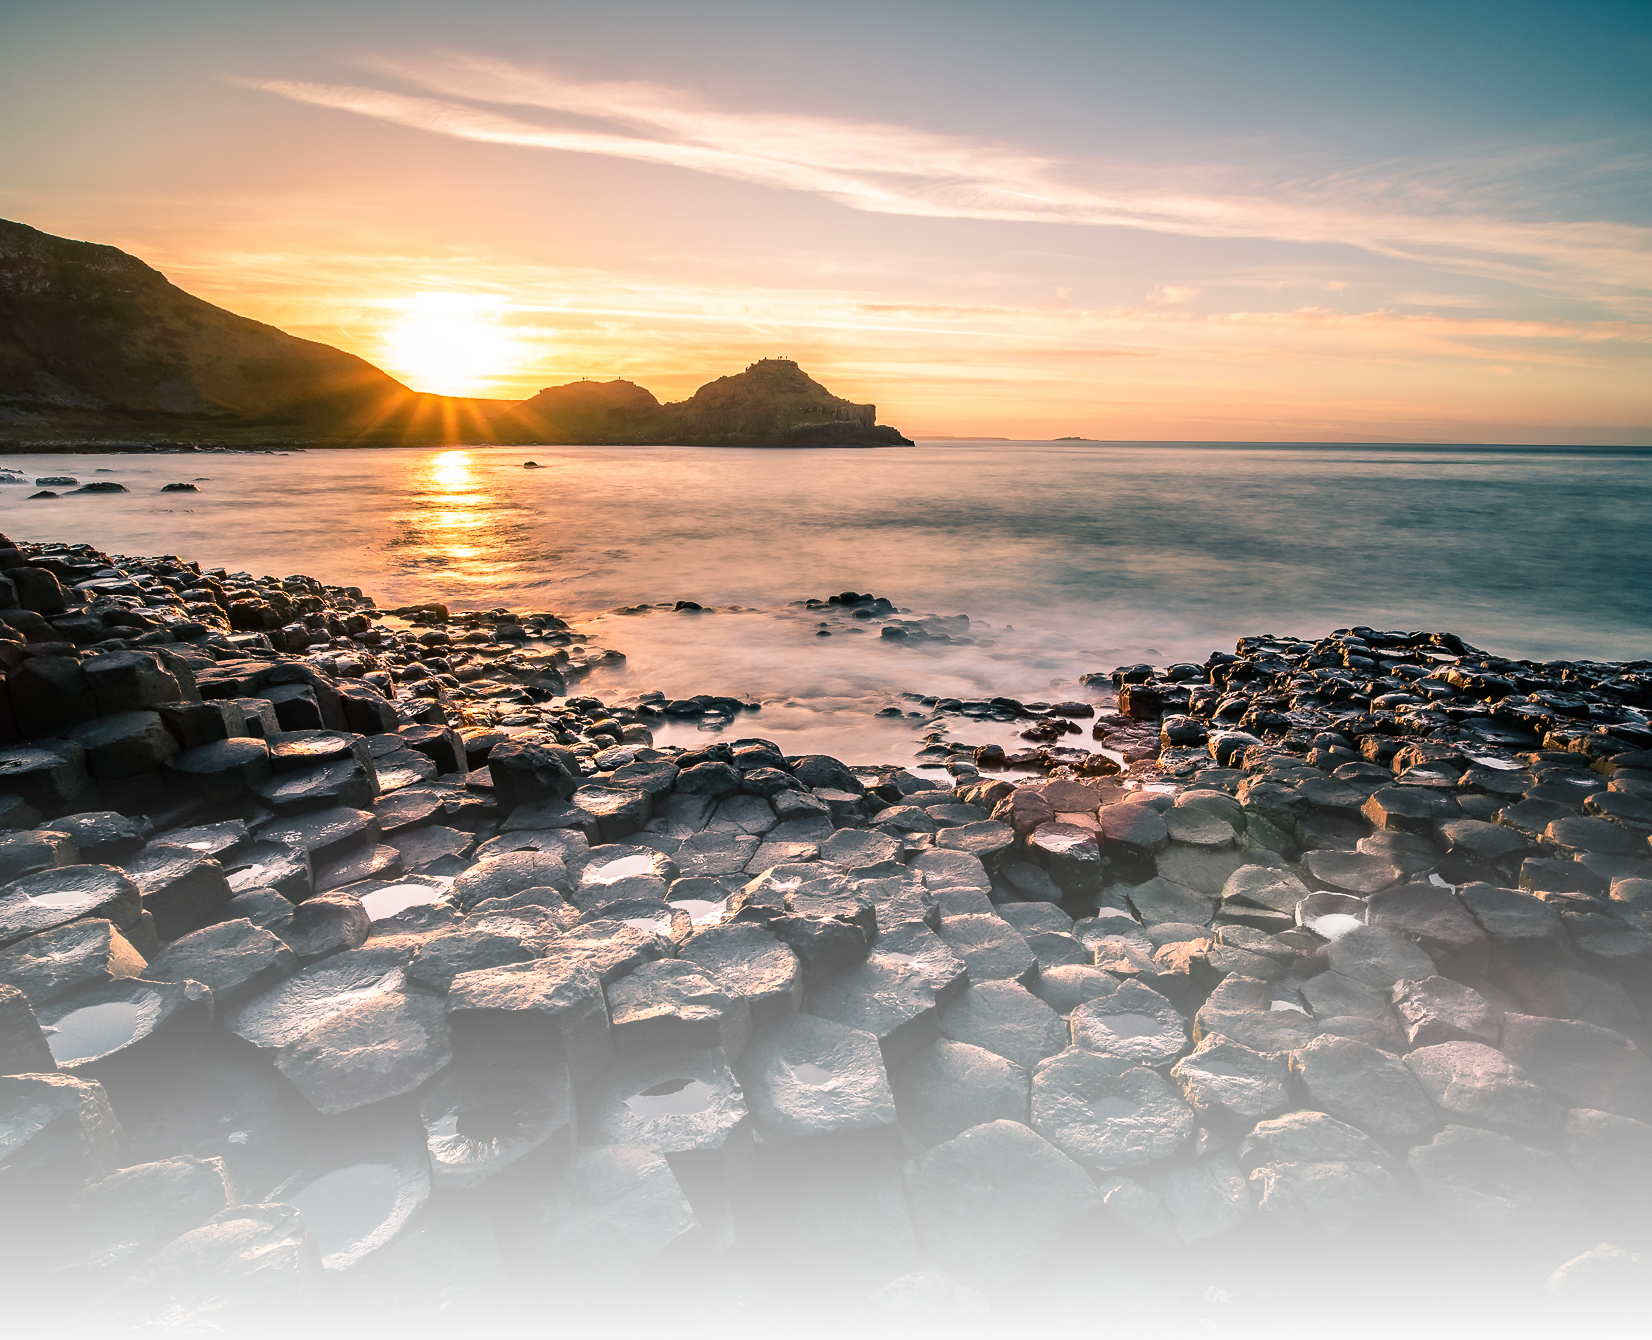
\includegraphics[width=635pt]{src/hexagons}}
};
\end{tikzpicture}
\vspace{1cm}

\textcolor{white}{
\titlefont Deep-Dive \\[0.3cm]
\subtitlefont Studies Into Mathematics\\[0.75cm]
\subsubtitlefont Luiz G. Mugnaini A.\\[0.75cm]Last Modification: \today
}
\end{center}
\newpage
\end{titlingpage}

%%% Local Variables:
%%% mode: latex
%%% TeX-master: "../deep-dive"
%%% End:

\maketitle

\tableofcontents
\listoftodos

\pagestyle{plain}

\chapter{Preface}

First of all I should stress that the title page template was taken from the
beautiful book~\cite{Haine21DiffCoho} by P. Haine et al.~--- the whole credit
should be given to them. The following text is a compilation of notes for my
studies in mathematics, that being said, it is clear that the collection of
mathematical and linguistic errors is non-empty. My main references are
\begin{itemize}\setlength\itemsep{0em}
\item Category Theory:~\cite{Rie16} and \cite{Shap06}.
\item Algebra:~\cite{Yu89},~\cite{Kim20},~\cite{Aluf09} and~\cite{Lang93}.
\item Topology:~\cite{Lee11},~\cite{Tai20},~\cite{Mun00} and~\cite{Eng89}.
\item Differential Structures:~\cite{Zor15},~\cite{Zor16},~\cite{Rud76}
  and~\cite{Jost06}.
\item Combinatorics:~\cite{Die16}.
\end{itemize}

\mainmatter

\part{Category theory}

\chapter{Categories}

\section{Characterizations and Morphisms}

\begin{definition}[Category]\label{def: category}
  A category \(\cat C\) consists of the following data
  \begin{enumerate}[(C1)]
    \item A collection of objects. We say that \(X\) is an object of \(\cat C\)
      by writing \(X \in \cat C\) or \(X \in \Obj(\cat C)\).
    \item For every given pair of objects \(X, Y \in \cat C\) there exists a
      collection of morphisms \(\Hom_{\cat C}(X, Y)\) with source \(X\) and
      target \(Y\). The collection of morphisms between objects of \(\cat C\) is
      denoted \(\Mor(\cat C)\).
    \item For every object \(X \in \cat C\), there exists an identity morphism
      \(\Id_X \in \Hom_{\cat C}(X, X)\).
    \item For every triple of given objects \(X, Y, Z \in \cat C\), there exists
      a composition map
      \[
        \Hom_{\cat C}(X, Y) \times \Hom_{\cat C}(Y, Z) \to \Hom_{\cat C}(X, Z).
      \]
      So that for given morphisms \(f \in \Hom_{\cat C}(X, Y)\) and \(g \in
      \Hom_{\cat C}(Y, Z)\) there exists a uniquely defined map \(g  f \in
      \Hom_{\cat C}(X, Z)\) such that the following diagram commutes
      \[
        \begin{tikzcd}
          Y \ar[r, "g"]
            &Z \\
          X \ar[u, "f"] \ar[ru, dashed, swap, "g  f"]
        \end{tikzcd}
      \]
    \item For every morphism \(f: X \to Y\) we have that
      \[
        \begin{tikzcd}
          X \ar[r, "f"] \ar[loop left, "\Id_X"] &Y \ar[loop right, "\Id_Y"]
        \end{tikzcd}
      \]
      so that \(\Id_Y  f = f = f  \Id_X\).
    \item Given ojects \(W, X, Y, Z \in \cat C\), the following diagram commutes
      \[
        \begin{tikzcd}
          W
          \ar[r, "f"]
          \ar[rr, bend right, swap, "g  f"]
          \ar[rrr, bend right = 50, swap, "h  (g  f)"]
          \ar[rrr, bend left = 50, "(h  g)  f"]
            &X
            \ar[r, "g"] \ar[rr, bend left, "h  g"]
              &Y
              \ar[r, "h"]
                &Z
        \end{tikzcd}
      \]
      that is, \(h  (g  f) = (h  g)  f\).
  \end{enumerate} \end{definition} \begin{definition}[Small]\label{def: small cat}
  A category \(\cat C\) is said to be small if it is composed of a set's worth
  of morphisms.
\end{definition}

\begin{definition}[Locally small]
  A category \(\cat C\) is said to be locally small if for any objects \(A,B
  \cat C\) there exists a set's worth of morphisms \(A\) and \(B\).
\end{definition}

\begin{corollary}[Unique identity]\label{cor: unique identity}
  Given a category \(\cat C\) and an object \(c \in \cat C\), the identity
  \(\Id_c \in \Mor(\cat C)\) is unique.
\end{corollary}

\begin{proof}
  Let \(f: c \to c\) be an identity of \(c\), then \(f = f \Id_c = \Id_c\).
\end{proof}

\begin{definition}
  Given a category \(\cat{C}\) and objects  \(A, B \in \cat{C}\), we
  define a morphism \(f \in \Hom(A, B)\) to be an \emph{isomorphism} if
  and only if it has a both sided inverse, so that exists \(f^{-1} \in
  \Hom(B, A)\) such that \(f^{-1}f = \Id_A\) and  \(ff^{-1} =
  \Id_B\).
\end{definition}

\begin{proposition}\label{prop: iso unique inverse}
   Given an isomorphism \(f\), its inverse is unique.
\end{proposition}

\begin{proof}
   Suppose for instance that there are two such functions, \(g, h \in
   \Hom(B, A)\), that act as an inverse for \(f \in \Hom(A,
   B)\). Note that
   \[
      g = g \Id_B = g(f h) = (g f) h = \Id_A h = h
   \]
   Thus \(g = h\) and therefore the inverse is indeed unique.
\end{proof}

\begin{definition}[Monoid]\label{def: monoid}
  A monoid is a set \(M\) equipped with a binary operation \(\otimes: M \times M
  \to M\) and a neutral element \(e \in M\). The binary operation is associative
  and obeys the right and left unit laws, that is
  \[
    x \otimes (y \otimes z) = (x \otimes y) \otimes z \qquad \text{ and } \qquad
    e \otimes x = x = x \otimes e.
  \]
\end{definition}

\begin{example}
  A monoid \(M\) defines a 1-category object category \(\cat{BM}\) such that
  \(\Obj(\cat{BM}) = \{*\}\) and \(\Hom_{\cat{BM}}(*, *) = \{*\}\). Composition
  of morphisms \(f, g: * \to *\) is defined as \(g  f = g \otimes f\). The
  identity morphism is \(\Id_* = e\). Hence we have \(e * f = f = f * e\) for
  all morphisms \(f \in \Mor(\cat{BM})\).
\end{example}

\begin{definition}[Groupoids]\label{def: groupoids}
  A \emph{groupoid} is the name given to a category in which all of its
  morphisms are isomorphisms.
\end{definition}

\begin{definition}[Group]\label{def: group}
  A group is a groupoid with one object.
\end{definition}

\begin{definition}[Automorphism]
  Given a category \(\cat C\) and an object  \(A \in \cat C\), we define an
  automorphism of \(A\) to be an isomorphism \(A \to A\). The set consisting of
  all such automorphisms of this object is denoted \(\Aut(A)\), the
  automorphisms have properties:
  \begin{enumerate}[i.]
    \item The composition of two automorphisms is an automorphism.
    \item Composition is associative.
    \item \(\Id_A \in \Aut(A)\).
    \item Every automorphism \(f \in \Aut(A)\) has an inverse \(f^{-1}
       \in \Aut(A)\).
  \end{enumerate}
  With this, the structure \(\Aut(A)\) is a \emph{group}, for all choices of
  objects \(A \in \cat{C}\).
\end{definition}

\begin{definition}[Subcategory]\label{def: subcategory}
  Let \(\cat C\) be a category. We define \(\cat D \subseteq \cat C\) as a
  subcategory of \(\cat C\) if: \(\Obj(\cat D)\) is a restriction of \(\Obj(\cat
  C)\); for all \(A \in \Obj(\cat D)\) there exists \(\Id_A \in \Mor(\cat D)\);
  for any \(f \in \Mor(\cat D)\) there exists \(\dom(f), \codom(f) \in
  \Obj(\cat D)\); for any composable pair of morphisms \(f, g \in \Mor(\cat D)\)
  there exists \(f g \in \Mor(\cat D)\).
\end{definition}

\begin{lemma}
  Any category \(\cat C\) contains a subcategory containing all of the objects
  and whose morphisms are only the isomorphisms. Such subcategory is called a
  maximal groupoid.
\end{lemma}

\begin{proof}
  We are going to prove that the maximal groupoid, name it \(\cat G\) is indeed
  a subcategory of \(\cat C\). Notice that \(\Obj(\cat G) = \Obj(\cat C)\),
  moreover every identity is an isomorphism, then \(\Id_{*} \in \Mor(\cat G)\).
  Let \(f \in \Mor(\cat G)\) then in particular we have \(f \in \Mor(\cat C)\)
  and hence \(\operatorname{dom} f, \operatorname{codom} f \in \Obj(\cat C) =
  \Obj(\cat G)\). Consider \(f \in \Hom_{\cat G}(A, B)\) and \(g \in \Hom_{\cat
  G}(B, C)\), composable isomorphisms, and notice that \(f^{-1}  g^{-1}
  \in \Hom_{\cat C}(C, A)\) is such that \((f^{-1}  g^{-1})  (g
  f) = \Id_A\) and \((g  f)  (f^{-1}  g^{-1}) = \Id_C\), hence we
  conclude that \(g  f\) is an isomorphism and therefore \(g  f \in
  \Hom_{\cat G}(A, C)\).
\end{proof}

\begin{definition}[Full subcategory]\label{def: full subcategory}
  A subcategory \(\cat D\) of \(\cat C\) (see \cref{def: subcategory}) is said
  to be a full subcategory if for all \(x, y \in \cat D\) we have \(\cat D(x, y)
  = \cat C(x, y)\).
\end{definition}

\begin{proposition}[Slice category]\label{prop: slice cat}
  Given a category \(\cat C\) and an object \(c \in \cat C\). The following
  define categories:
  \begin{enumerate}[(SC1)]
    \item\label{prop: slice under}
      (Slice under \(c\)) A category \(c/\cat C\), called slice category of
      \(\cat C\) under \(c\), whose objects are morphisms \(f \in \Hom_{\cat
      C}(c, *)\). Given objects \(f, g \in c/\cat C\) such that \(f: c \to x\)
      and \(g: c \to y\), we define a morphism \(f \to g\) as a map \(h: x \to
      y\) such that the following diagram commutes
      \[
        \begin{tikzcd}
          &c \ar[dl, swap,"f"] \ar[dr, "g"]\\
          x \ar[rr, "h"] & &y
        \end{tikzcd}
      \]
      that is, \(g = h  f\).
    \item\label{prop: slice over}
      (Slice over \(c\)) A category \(\cat C/c\), called the slice category of
      \(\cat C\) over \(c\), whose objects are morphisms \(f \in \Hom_{\cat
      C}(*, c)\). Morphisms between objects \(f, g \in \cat C/c\) such that \(f:
      x \to c\) and \(g: y \to c\) are maps \(h: x \to y\) such that the
      following diagram commutes
      \[
        \begin{tikzcd}
          x \ar[rr, "h"]
            & &y \\
            &c \ar[ul, "f"] \ar[ur, swap, "g"]
        \end{tikzcd}
      \]
      so that \(f = g  h\).
  \end{enumerate}
\end{proposition}

\begin{proof}
  (SC1) Given objects \(f, g \in c/\cat C\) we have from construction that
  \[
    \Hom_{c/\cat C}(f, g) = \Hom_{\cat C}(\codom f, \codom g),
  \]
  hence we are
  ensured of the existence of such morphisms between objects. Given an object
  \(f: c \to x\), the morphism \(\Id_x \in \Mor(\cat C)\) is such that \(f =
  \Id_x  f\), so that \(\Id_x\) is the identity morphism for \(f\). Let
  \(f, g, u \in c/\cat C\) be objects such that \(f: c \to x,\ g: c \to y,\ u: c
  \to z\), then there exists morphisms \(h \in \Hom_{c/\cat C}(f, u)\) and
  \(\ell: \Hom_{c/\cat C}(u, g)\) so that the following diagram commutes
  \[
    \begin{tikzcd}
        &c \ar[dl, swap, "f"] \ar[d, "u"] \ar[dr, "g"] & \\
      x \ar[r, "h"]
        &z \ar[r, "\ell"]
          &y
    \end{tikzcd}
  \]
  so that we have a uniquely defined morphism \(\ell  h \in \Hom_{\cat
  C}(x, y)\), where in particular \(\ell  h \in \Hom_{c/\cat C}(f, g)\) and
  thus this defines a map \(\Hom_{c/\cat C}(f, u) \times \Hom_{c/\cat C}(u, g)
  \to \Hom_{c/\cat C}(f, g)\). Since \(\Id_x, \Id_z \in \Mor(c/\cat C)\) for any
  \(x, y \in \cat C\), then given \(f, u \in c/\cat C\) just as above, the
  morphism \(h: x \to z\) is such that \(\Id_z  h = h = h  \Id_x\). In
  addition to the objects and morphisms named above, define \(v: c \to w\) and
  the corresponding morphism \(t \in \Hom_{c/\cat C}(g, v)\) so that \(t: y \to
  w\) and \(v = t  g\). From the fact that \(\cat C\) is a category, we
  find that \((t  \ell)  h = t  (\ell  h)\) and hence the
  same is true for \(c/\cat C\).

  (SC2) Let \(f, g \in \cat C/c\), then from definition we have \(\Hom_{\cat
  C/c}(f, g) = \Hom_{\cat C}(\dom f, \dom g)\), which is well defined on \(\cat
  C\). Given an object \(f: x \to c\), there exists \(\Id_x: x \to x\) so that
  \(f = f  \Id_x\) and hence \(\Id_x\) is the identity morphism for \(f\).
  Define objects \(f, g, u \in \cat C/c\) such that \(f: x \to c,\ g: y \to c,\
  u: c \to z\), and morphisms \(h \in \Hom_{\cat C/c}(u, f)\) and \(\ell \in
  \Hom_{\cat C/c}(g, u)\). Then, the following diagram commutes
   \[
    \begin{tikzcd}
      x
        &z \ar[l, swap, "h"]
          &y \ar[l, swap, "\ell"] \\
        &c \ar[lu, "f"] \ar[u, "u"] \ar[ru, swap, "g"]
    \end{tikzcd}
  \]
  hence the morphism \(h  \ell \in \Hom_{\cat C}(y, x)\) defines a morphism
  \(h  \ell \in \Hom_{\cat C/c}(g, f)\) so that we can construct a map well
  defined map \(\Hom_{\cat C/c}(g, u) \times \Hom_{\cat C/c}(u, f) \to
  \Hom_{\cat C/c}(g, f)\). Moreover, given \(f\) and \(u\) as above, we have
  that there exists \(\Id_x, \Id_z \in \Mor(\cat C/c)\) so that from the
  category \(\cat C\) it follows that \(\Id_x  h = h  \Id_z\). In
  addition to the above, define \(v: w \to c\) and the morphism \(t \in
  \Hom_{\cat C/c}(v, g)\) so that \(t: w \to y\). Then we have \(g = t  v\)
  and since \(\cat C\) is a category, we find that \((h  \ell)  t = h
   (\ell  t)\).
\end{proof}

\section{Duality}

\begin{definition}[Opposite category]\label{def: opposite cat}
  Let \(\cat C\) be a category. We define the opposite category of \(\cat C\) as
  \(\cat C^\op\), such that
  \begin{enumerate}[(COP1)]\setlength\itemsep{0em}
    \item \(\Obj(\cat C^\op) = \Obj(\cat C)\).
    \item Given a morphism \(f: x \to y\) in  \(\cat C\), there exists a
      corresponding morphism \(f^\op: y \to x\) in the \(\cat C^\op\). That is
      \(\dom f = \codom f^\op\) and \(\codom f = \dom f^\op\), these form all of
      the morphisms in the category \(\cat C^\op\).
    \item For all \(A \in \cat C^\op\), there exists an identity morphism
      \(\Id_A^\op \in \End_{\cat C^\op}(A)\).
    \item A pair of morphisms \(f^\op, g^\op \in \cat C^\op\) is composable, so
      that \(\dom g^\op = \codom f^\op\), if and only if the pair \(g, f \in
      \cat C\) is composable, that is \(\dom f = \codom g\). Moreover, we
      define their composition as \(g^\op f^\op = (f g)^\op\).
  \end{enumerate}
\end{definition}

\begin{lemma}\label{lem:f-iso-iff-f*-iso}
  The following propositions are equivalent
  \begin{enumerate}[(a)]\setlength\itemsep{0em}
    \item \(f : x \isoto y\) is an isomorphism in \(\cat C\).
    \item For all \(c \in \cat C\), the map
      \[
        f_*: \Hom_{\cat C}(c, x) \to \Hom_{\cat C}(c, y), \qquad
        g \xmapsto{f_*} f g
      \]
      is a bijection.
    \item For all \(c \in \cat C\), the map
      \[
         f^* : \Hom_{\cat C} (x, c) \to \Hom_{\cat C}(y, c), \qquad
         g \xmapsto{f^*} g f
      \]
      is a bijection.
  \end{enumerate}
\end{lemma}

\begin{proof}
  ((a) \(\Rightarrow\) (b)) Let \(f: x \isoto y\) be an isomorphism and \(c
  \in \cat C\) be an object and define \(\ell : y \isoto x\) to be its inverse.
  Given \(c \in \cat C\), define \(\ell_*: \Hom_{\cat C}(c, y) \to \Hom_{\cat
  C}(c, x)\). Notice that \(f_* \ell_* : \Hom_{\cat C}(c, y) \to
  \Hom_{\cat C}(c, y)\) mapping \(g \mapsto f_*(\ell_*(g)) = f \ell
  g = g\), hence \(f_* \ell_* = \Id_{\Hom_{\cat C}(c, y)}\). Moreover, we
  have \(\ell_* f_* : \Hom_{\cat C}(c, x) \to \Hom_{\cat C}(c, x)\) mapping \(h \mapsto
\ell_*(f_*(h)) = h f \ell = h\), hence
  \(\ell_* f_* = \Id_{\Hom_{\cat C}(c, x)}\). This shows that \(\ell_*\)
  is the inverse of \(f_*\) and therefore \(f_*\) is an isomorphism. ((b)
  \(\Rightarrow\) (a)) Suppose the contrary, so that \(f_*\) is an isomorphism.
  In particular, we can take \(c = y\) so that \(f_*: \Hom_{\cat C}(y, x) \to
  \Hom_{\cat C}(y, y)\). From the isomorphism property, there exists \(\ell \in
  \Hom_{\cat C}(y, x)\) such that \(f_*(\ell) = f \ell = \Id_y\). Consider
  now that \(c = x\), then \(f_*: \Hom_{\cat C}(x, x) \to \Hom_{\cat C}(x, y)\).
  Notice that \(f_*(\ell f) = f \ell f = \Id_y f = f\)
  and \(f_*(\Id_x) = f \Id_x = f\). Since \(f_*\) is supposed to be an
  isomorphism, it follows that \(\Id_x = \ell f\). With this we conclude
  that \(\ell\) is the inverse of \(f\) and hence \(f\) is an isomorphism.

  ((a) \(\Leftrightarrow\) (c)) Suppose that \(f^\op: y \to x \in \cat
  \Mor(C^\op)\), then from the last paragraph we have that \(f^\op\) is an
  isomorphism if and only if \((f^\op)_* : \Hom_{\cat C^\op}(c, y) \to
  \Hom_{\cat C^\op}(c, x)\) is an isomorphism. Therefore the dual of such
  statement is that \(f: x \to y \in \cat \Mor(C)\) is an isomorphism if and
  only if \((f^\op)_*^\op = f^*: \Hom_{\cat C}(x, c) \to \Hom_{\cat C}(y, c)\)
  is an isomorphism, since \(\Hom_{\cat C^\op}(*, *') = \Hom_{\cat C}(*', *)\).
\end{proof}

\begin{definition}[Monomorphism]\label{def: monomorphism}
  Let a category \(\cat{C}\). We say that \(f \in \Hom_{\cat C}(x, y)\) is a
  \emph{monomorphism} if for all \(c \in \cat{C}\), and for all \(\alpha, \beta
  \in \mathrm{Hom}(c, x)\) we have that \(f \alpha = f \beta\) implies \(\alpha
  = \beta\). Equivalently, for all \(c \in \cat C\) the map \(f_*: \Hom_{\cat
  C}(c, x) \to \Hom_{\cat C}(c, y)\) is injective.
\end{definition}

\begin{definition}[Epimorphism]\label{def: epimorphism}
  Let a category \(\cat C\). We say that morphism \(g \in \mathrm{Hom}_{\cat
  C}(x, y)\) to be an \emph{epimorphism} if for all \(c \in \cat{C}\), and for
  all \(\gamma, \delta \in \mathrm{Hom}_{\cat C}(y, c)\) we have that \(\gamma g
  = \delta g\) implies \(\gamma = \delta\). Equivalently, for all \(c \in \cat
  C\) the map \(g^*: \Hom_{\cat C}(y, c)\to \Hom_{\cat C}(x, c)\) is injective.
\end{definition}

\begin{proposition}
\label{prop:}
Let \(\cat C\) be a category. The following are properties regarding
monomorphisms and epimorphisms in \(\cat C\):
\begin{enumerate}[(a)]\setlength\itemsep{0em}
\item Every identity morphism is a monomorphism and an epimorphism
\item The composite of two monomorphisms (or epimorphisms) is a monomorphism (or
  epimorphism).
\item If the composition \(k f\) is a monomorphism, then \(f\) is a
  monomorphism. Conversely, if \(f k\) is an epimorphism, then \(f\) is an
  epimorphism.
\end{enumerate}
\end{proposition}

\begin{proof}
We prove the assertions about monomorphisms, the respective ones for
epimorphisms are dually true from the former.
\begin{enumerate}[(a)]\setlength\itemsep{0em}
\item Identities are isomorphism, so clearly they are monomorphisms and
  epimorphisms.

\item Let \(f\) and \(g\) be composable monomorphisms, then if \(g f p = g f q\)
  for two given morphisms \(p\) and \(q\), for since \(g\) is a monomorphism
  then \(f p = f q\) --- then using the fact that \(f\) is a monomorphism we
  obtain \(p = q\).

\item Suppose \(k f\) is a monomorphism and consider morphisms \(g\) and \(h\)
  such that \(f g = f h\). Composing with \(k\) one sees that \(k f g = k f h\)
  but since \(k f\) is a monomorphism, it follows that \(g = h\).
\end{enumerate}
\end{proof}

\begin{definition}
  Let \(x \xrightarrow s y \xrightarrow r x\) be morphisms such that \(r s =
  \Id_x\). We define the following terms
  \begin{enumerate}[(a)]\setlength\itemsep{0em}
    \item\label{def: split monomorphism}
      \(s\) is said to be a section of \(r\). The morphism \(s\) is always a
      monomorphism, being called a split monomorphism.
    \item\label{def: split epimorphism}
      \(r\) is said to be the retraction of \(s\). The morphism \(r\) is always
      an epimorphism, being called a split epimorphism.
    \item\label{def: retract}
      \(x\) is the retract of \(y\).
  \end{enumerate}
\end{definition}

\begin{proposition}
  A morphism \(f \in \Hom_{\cat C}(x, y)\) is a split epimorphism if and only if
  for all \(c \in \cat C\) the map \(f_*: \Hom_{\cat C}(c, x) \to \Hom_{\cat
    C}(c, y)\) is surjective. Dually, \(f\) is a split monomorphism if and only
    if for all \(c \in \cat C\) the map \(f^*: \Hom_{\cat C}(x, c) \to
    \Hom_{\cat C}(y, c)\) is surjective.
\end{proposition}

\begin{proof}
  (\(\Rightarrow\)) Suppose \(f: x \to y\) is a split epimorphism and define
  \(g: y \to x\) as a section of \(f\), that is \(f g = \Id_y\). Let \(c
  \in \cat C\), and \(\alpha \in \Hom_{\cat C}(c, y)\) be any morphism. Notice
  that \(g \alpha \in \Hom_{\cat C}(c, x)\), hence we find that \(f_*(g
  \alpha) = f g \alpha = \alpha\) and therefore \(f_*\) is
  surjective. (\(\Leftarrow\)) Suppose \(f_*\) is surjective, then in particular
  for \(c = y\) we have that \(\Id_y \in \im f_*\) and hence \(f\) is a split
  epimorphism. (Dual) Let \(f^\op: y \to x\), then from the above proposition
  \(f^\op\) is a split epimorphism if and only if \((f^\op)_*: \Hom_{\cat
  C^\op}(y, c) \to \Hom_{\cat C^\op}(x, c)\) is surjective. Dually we have that
  \(f\) is a monomorphism if and only if \((f^\op)_*^\op = f^*: \Hom_{\cat C}(c,
  x) \to \Hom_{\cat C}(c, y)\), which proves the last part.
\end{proof}

\begin{proposition}
  Let \(f \in \Mor(\cat C)\). If \(f\) is a monomorphism and also a split
  epimorphism, then \(f\) is an isomorphism. Dually, if \(f\) is an epimorphism
  and a split monomorphism, then \(f\) is an isomorphism.
\end{proposition}

\begin{proof}
  Suppose \(f: x \to y\) is a split epimorphism and \(g: y \to x\) be a section
  of \(f\), then \(f g = \Id_y\) and, moreover \(f g f = \Id_y
  f = f\) hence from if \(f\) is a monomorphism we conclude that \(g
  f = \Id_x\). Thus \(g\) is the inverse of \(f\) and hence \(f\) is an
  isomorphism. Dually, let \(f^\op: y \to x\) be a monomorphism and split
  epimorphism, then \(f^\op\) is an isomorphism, which dually means that \(f\)
  is an epimorphism and split monomorphism, then \(f\) is an isomorphism.
\end{proof}

\begin{lemma}
  Let \(f: x \to y\) and \(g: y \to z\). The following propositions hold
  \begin{enumerate}[(a).]\setlength\itemsep{0em}
    \item If \(f\) and \(g\) are monomorphisms, so is \(g f: x \mono z\).
      For the dual proposition, if \(f\) and \(g\) are epimorphisms, then \(g
      f: x \epi z\) is an epimorphism.
    \item If \(g f: x \mono z\) is a monomorphism, then \(f\) is also
      monomorphism.  Dually, if \(g f: x \epi z\) is an epimorphism, then
      \(g\) is an epimorphism.
  \end{enumerate}
\end{lemma}

\begin{proof}
  (a) Suppose that \(f, g\) are both monomorphisms. Given any \(c \in \cat C\),
  let \(\alpha, \beta \in \Hom_{\cat C}(c, x)\) be such that \(g f \alpha = g f
  \beta\). In particular, since \(g\) is monic, then \(f \alpha = f \beta\), but
  \(f\) is also monic, hence \(\alpha = \beta\). For the dual part, suppose that
  \(f^\op: y \to x\) and \(g^\op: z \to y\) be monic, then from above we have
  \(f^\op g^\op = (g f)^\op\) monic, which dually implies that \(g f\) is epic.

  (b) Let \(g f\) be monic. Then given \(c \in \cat C\) and \(\alpha, \beta \in
  \Hom_{\cat C}(c, x)\) such that \(f \alpha = f \beta\), then in particular
  \(g(f \alpha) = g(f \beta)\), then from the monic property we have \(\alpha =
  \beta\). Dually, suppose that \((g f)^\op = f^\op g^\op \in \Mor(\cat C^\op)\)
  is monic, then from above we find that \(g^\op\) is monic, which dually
  implies that \(g\) is epic.
\end{proof}

\section{Functors}

\begin{definition}[Functor]\label{def: functor}
Let \(\cat C\) and \(\cat D\) be categories. A functor \(F: \cat C \to \cat
D\) has the following data:
\begin{enumerate}[({DF}1)]
  \item For all \(c \in \cat C\) exists a corresponding \(F c \in \cat D\).
  \item For all \(f: c \to c' \in \Mor(\cat C)\) there exists a morphism \(F
    f: F c \to F c' \in \Mor(\cat D)\).
\end{enumerate}
Such data satisfies the two following axioms:
\begin{enumerate}[({AF}1)]
  \item For all composable \(f, g \in \Mor(\cat C)\), we have \(F g \cdot F f
    = F (g \cdot f)\).
  \item For all \(c \in \cat C\) we have \(F \Id_c = \Id_{F c} \in \Mor(\cat
    D)\).
\end{enumerate}
This definition is sometimes called covariant functor (in contrast with
contravariant functor, see \cref{def: contravariant functor}).
\end{definition}

\begin{definition}[Forgetful functor]
A functor is said to be forgetful if the functor ``forgets'' some object,
structure or property of its domain category.
\end{definition}

\begin{example}
We have some classical examples of forgetful functors, for instance, the
following are functors that forget the structure of their domain categories:
\begin{itemize}
  \item The functor \(G: \Grp \to \Set\) mapping groups to its
    corresponding underlying set.
  \item The functor \(T: \Top \to \Set\) maps any topological space
    to its corresponding set of points.
  \item The functor \(V, E: \Graph \to \Set\) maps the vertices and
    edges of a graph to the set of such vertices an edges.
\end{itemize}
\end{example}

\begin{definition}[Contravariant functor]
\label{def: contravariant functor}
A contravariant functor from categories \(\cat C\) to \(\cat D\) is a functor
\(F: \cat C^\op \to \cat D\) together with the following data:
\begin{enumerate}[({DCF}1)]
  \item For all \(c \in \cat C\) exists \(F c \in \cat D\).
  \item For all \(f: c \to c' \in \Mor(\cat C)\) we have \(F f: F c' \to F c
    \in \Mor(\cat D)\).
\end{enumerate}
Moreover, a contravariant functor satisfies the following axioms:
\begin{enumerate}[({ACF}1)]
  \item For all composable \(f, g \in \Mor(\cat C)\) we have \(F f \cdot F g =
    F (g \cdot f)\).
  \item For all \(c \in \cat C\) we have \(F \Id_c = \Id_{F c}\).
\end{enumerate}
This can all be comprised diagrammatically as:
\[
  \begin{tikzcd}
    \cat C^\op \ar[rr, "F"] & &\cat D
    \\
    c \ar[d, "f"] \ar[dd, bend right = 60, swap, "g f"]
    \ar[rr, mapsto]
    & &F c
    \\
    c' \ar[d, "g"] \ar[rr, mapsto]
    & &F c' \ar[u, "F f"]
    \\
    c'' \ar[rr, mapsto]
    & & F c''
    \ar[u, "F g"]
    \ar[uu, bend right = 60, swap, "F f \cdot F g = F (g \cdot f)"]
  \end{tikzcd}
\]
\end{definition}

\begin{example}[\(\Top^\op \to \Rng\)]
Let \(C: \Top^\op \to \Rng\) be a contravariant functor such that
for all \(X \in \Top\), let \(C X\) be the ring of continuous functions
\(X \to \R\). The ring operations on \(C X\) are defined pointwise,
that is, given \(p, q: X \to \R \in C X\) we have \((p \cdot q) (x) =
p(x) \cdot q(x)\) and \((p + q)(x) = p(x) + q(x)\) for all \(x \in X\).
Moreover, given a morphism \(f: X \to Y \in \Mor(\Top)\) we define \(C f:
C Y \to C X\) as the composition \((C f)(q) = q f \in \Mor(C X)\) for all \(q
\in C Y\), that is
\[
  \begin{tikzcd}
    X \ar[r, "f"] \ar[rr, bend right = 40, swap, "C f(q) = q f"]
    & Y \ar[r, "q"] & \R
  \end{tikzcd}
\]

We now show that the axioms for the contravariant functor are satisfied by
\(C\). Let \(f: X \to Y\) and \(g: Y \to Z\), then given any \(p \in C Z\) we
have
\[
  \begin{tikzcd}
    X \ar[r, "f"]
    \ar[rrr, bend left = 60, "C f(C g (p))"]
    \ar[rrr, bend right, swap, "C (g f)(p)"]
    & Y \ar[r, "g"]
    \ar[rr, bend left = 35, "C g(p)"]
    & Z \ar[r, "p"] & \R
  \end{tikzcd}
\]
hence \(C (f) C (g) = C (g f)\). Moreover, given any \(X \in \Top^\op\)
we find that \(C \Id_X: C X \to C X\) is such that for all \(q \in C X\), \(C
\Id_X (q) = q \Id_X = q\) hence \(C \Id_X = \Id_{C X}\). This finishes the
proof that \(C: \Top^\op \to \Rng\) is a contravariant functor.
\end{example}

\begin{definition}[Presheaf]\label{def: presheaf}
Let \(\cat C\) be a small category. A contravariant functor \(\cat C^\op \to
\Set\) is called a presheaf on \(\cat C\).
\end{definition}

\begin{example}[\(\mathcal O(X)^\op \to \Set\)]
Let \(X \in \Top\) we define \(\mathcal O(X)\) to be the poset category
whose objects are open sets of \(X\). That is, for sets \(U, U' \in \mathcal
O(X)\), if \(U \subseteq U'\), then there exists a morphism \(U \to U'\) in
\(\Mor(\mathcal O(X))\). A presheaf on the category \(\mathcal O(X)\) is a
functor \(F: \mathcal O(X)^\op \to \Set\) that assigns \(F U = \{f: U \to
\R: f \text{ continuous}\}\) for all \(U \in \mathcal O(X)\).
Moreover, for maps \(g: U \to U'\) (that is \(U \subseteq U'\)) we have \(F g:
F U' \to F U\) such that \(F g(f) = f|_U: U \to \R\) for all \(f: U'
\to \R\) continuous. Since the restriction of a continuous map is
continuous, then \(f|_U \in F U\)
\end{example}

\begin{example}[Simplex category]
\label{exp:simplex-category}
The simplex category \(\Delta\) comprises objects that are finite non-empty
ordinals and order-preserving morphisms. Simplicial sets are defined as
presheaves \(\Delta^{\op} \to \Set\).
\end{example}

\begin{lemma}\label{lem: functor preserve iso}
Functors preserve isomorphisms. Let \(\cat C\) and \(\cat D\) be categories
and \(F: \cat C \to \cat D\) be a functor. Given an isomorphism \(f: c \isoto
c' \in \Mor(\cat C)\), we have that \(F f : F c \isoto c'\) is an isomorphism.
\end{lemma}

\begin{proof}
Denote by \(f^{-1}: c' \isoto c\) the inverse of \(f\). By the composition
axiom we have
\begin{gather*}
  F (f^{-1}) F (f) = F (f^{-1} f) = F \Id_c    = \Id_{F c}, \\
  F (f) F (f^{-1}) = F (f f^{-1}) = F \Id_{c'} = \Id_{F c'}.
\end{gather*}
This shows that \(F f^{-1}\) is the right and left inverse of \(F f\), hence
\(F f: F c \isoto F c'\) is indeed an isomorphism.
\end{proof}

\begin{example}[Group action]\label{exp:grp-action}
Let \(G\) be any group and consider the category \(\cat{B}G\) generated by \(G\)
--- that is, \(\cat BG\) consists of a unique object \(*\) and the morphisms of
the category are endomorphisms \(* \to *\) given by the elements of \(G\). Given
a category \(\cat C\), a functor \(X: \cat BG \to \cat C\) --- given by mapping
\(X* \coloneq X \in \cat C\) and each object \(g \in G\) to an endomorphism \(Xg
\coloneq g_{*}: X \to X\) --- is said to define a left group action on the
object \(X \in \cat C\). Moreover, the functor \(X\) has to obey
\begin{itemize}\setlength\itemsep{0em}
\item Composition preserving: for any \(h, g \in G\), we have \((h g)_{*} =
  h_{*} g_{*}\).
\item Identity: \(e_{*} = \Id_X\).
\end{itemize}
Since functors preserve isomorphisms and every morphism of \(\cat BG\) is an
automorphism, it follows that, for all \(g \in G\), the map \(g_{*}: X \to X\)
is an automorphism --- in particular, this implies that \((g^{-1})_{*} =
g_{*}^{-1}\).

Some particular cases of interest are the following:
\begin{itemize}\setlength\itemsep{0em}
\item If \(\cat C = \Set\), then the set \(X\) together with the actions
  \(\{g_{*} : g \in G\}\) is called a \(G\)-set.
\item If \(\cat C = \Vect_k\), then the \(k\)-vector space \(X\) together with
  the actions generated by \(G\) is said to be a \(G\)-representation.
\item If \(\cat C = \Top\), then the topological space \(X\) endowed with the
  actions generated by \(G\) is called a \(G\)-space.
\end{itemize}

A right group action is nothing more than a contravariant functor \(X: \cat
BG^{\op} \to \cat C\) such that \(X* \coloneq X\) and \(Xg \coloneq g^{*}: X \to
X\) are endomorphisms. The rules for such a functor are the contravariant
preservation of compositions, that is, \((h g)_{*} = g_{*} h_{*}\), and that
\(e^{*} = \Id_X\) as before.
\end{example}

\begin{lemma}\label{lem: func-preserve-split}
Functors preserve split monomorphisms and split epimorphisms.
\end{lemma}

\begin{proof}
Let \(\cat C\) and \(\cat D\) be categories and consider a functor \(F: \cat C
\to \cat D\). Define morphisms \(x \xrightarrow s y \xrightarrow r x\) in
\(\Mor(\cat C)\) such that \(r s = \Id_x\), that is, \(s\) is a split
monomorphism and \(r\) is a split epimorphism. Consider the morphisms \(F s: F
x \to F y\) and \(F r: F y \to F x\) in \(\Mor(\cat D)\). Notice that \(F (s)
F(r) = F(s r) = F(\Id_x) = \Id_{F x}\). Hence \(F s\) is a split monomorphism
and \(F r\) is a split epimorphism.
\end{proof}

\begin{definition}[\(\Hom\) functors]\label{def:hom-functors}
Let \(\cat C\) be a locally small category. Given any \(c \in \cat C\), there
exists a pair of covariant and contravariant functors, \(\Hom(c, -)\) and
\(\Hom(-, c)\), respectively --- represented by the object \(c\). That is:
\[
  \begin{tikzcd}
    \cat C \ar[rr, "\Hom{(c, -)}"] & & \Set
    \\
    x \ar[rr, maps to] \ar[d, swap, "f"]
    & & \Hom(c, x) \ar[d, "f_*"]
    \\
    y \ar[rr, maps to] & & \Hom(c, y)
  \end{tikzcd}
  \qquad
  \begin{tikzcd}
    \cat C^\op \ar[rr, "\Hom{(-, c)}"] & & \Set
    \\
    x \ar[rr, maps to] \ar[d, swap, "f"]
    & & \Hom(x, c)
    \\
    y \ar[rr, maps to] & & \cat \Hom(y, c) \ar[u, swap, "f^*"]
  \end{tikzcd}
\]
\end{definition}

We now prove that such definition indeed satisfies the axioms for covariant and
contravariant functors. Given morphisms \(f: x \to y\) and \(g: y \to z\) in
\(\Mor(\cat C)\), we see that \(g_* f_* = (g f)_*\), moreover \(f^* g^* = (f
g)^*\). Let \(x \in \cat C\) be any object, then \(\Id_{x *} = \Id_{\Hom(c, x)}
= \Id_x^*\). This proves that \(\Hom(c, -)\) is covariant and \(\Hom(-, c)\) is
contravariant.

\begin{definition}[Faithful]\label{def: faithful}
Let \(\cat C\) and \(\cat D\) be categories. A functor \(F: \cat C \to \cat D\)
is said to be faithful if for all \(x, y \in \cat C\) the map \(\cat C(x, y) \to
\cat D(F x, F y)\) is injective.
\end{definition}

\begin{definition}[Full]\label{def: full}
Let \(\cat C\) and \(\cat D\) be categories. A functor \(F: \cat C \to \cat D\)
is said to be full if for all \(x, y \in \cat C\) the map \(\cat C(x, y) \to
\cat D(F x, F y)\) is surjective.
\end{definition}

\begin{definition}[Product category]\label{def:product-category}
Given categories \(\cat C\) and \(\cat D\), we define their product \(\cat C
\times \cat D\) to be a category whose objects are ordered pairs \((c, d)\) such
that \(c \in \cat C\) and \(d \in \cat D\), and morphisms are ordered pairs
\((f, g): (c, d) \to (c', d')\), where \(f: c \to c' \in \Mor(\cat C)\) and \(g:
d \to d' \in \Mor(\cat D)\). Composable morphisms \((f, g)\) and \((h, q)\) have
composition defined componentwise, that is, \((f, g) (h, q) = (fh, gq)\).
\end{definition}

\begin{definition}[Two sided represented functor]
\label{def:two-sided-represented-functor}
Let \(\cat C\) be a locally small category, then there is a functor \(\Hom(-,
-): \cat C^{\op} \times \cat C \to \Set\) defined by mapping objects \((x, y)
\mapsto \Hom(x, y)\) and morphisms \((f, g): (a, y) \to (x, b)\) to a
set-function \((f^{*}, g_{*}): \Hom(x, y) \to \Hom(a, b)\) given by the mapping
\(g \mapsto h g f\).
\end{definition}

Categories also form a category, whose objects are categories and morphisms are
functors between them --- but this gives rise to size \todo{describe}issues, so
we have to distinguish between two kinds of categories, the ones that are
\emph{small} and \emph{locally small}. This gives rise to two categories,
\(\Cat\) and \(\CAT\), comprised of objects that are small and locally small,
respectively.

\begin{definition}[Isomorphism of categories]
\label{def:isomorphism-categories}
Let \(\cat C\) and \(\cat D\) be categories. We say that \(\cat C\) is
isomorphic to \(\cat D\) if there exists morphisms \(F: \cat C \to \cat D\) and
\(G: \cat D \to \cat C\) such that \(GF = \Id_{\cat C}\) and \(FG = \Id_{\cat D}\).
\end{definition}

\begin{example}[Orbit category]
\label{exp:orbit-category}
Let \(G\) be a group. We define the orbit category associated to \(G\) as
\(\mathcal{O}_G\) whose objects are subgroups \(H \subseteq G\), identified by
the left \(G\)-set \(G/H\) of left costs of \(H\). The morphisms \(\phi: G/H \to
G/Q\) are maps commuting with the left \(G\)-action, that is, \(\phi(g_{*}h) =
g_{*} \phi(h)\) --- such maps are called \(G\)-equivariant.
\end{example}



%\begin{proposition}[Bifunctor]
%Let categories \(\cat A, \cat B\) and \(\cat C\). There exists a uniquely
%defined functor \(F: \cat A \times \cat B \to \cat C\).
%\end{proposition}

\todo[inline]{Bifunctor and two sided represented functor!}

\todo[inline]{After solving some problems on functors, next topic: natural
transformations}


\chapter{Limits}

\section{Universal Properties}

\subsection{Initial and final objects}

\begin{definition}[Initial and Final]\label{def: initial and final objects}
   Given a category \(\cat C\), an object \(I \in \cat C\) is said to be an
   \emph{initial object} in the category \(\cat{C}\) if for all \(A \in
   \cat C\), there exists exactly one morphism \(f \in \Hom(I, A)\) so that
   \(\Hom(I, A) = f\). Conversely, an object \(F \in \cat C\) is said to be an
   \emph{final object} in \(\cat C\) if there is exactly one morphism \(g \in
   \Hom(A, F)\) for all given \(A \in \cat C\) and thus \(\Hom(A, F) = g\).
\end{definition}

\begin{proposition}
   Let a category \(\cat{C}\), then initial and final objects are said to be
   unique up to a unique isomorphism:
   \begin{enumerate}[I.]
      \item If \(I',I'' \in \Obj(\cat{C})\) are initial objects of the
         category, then \(I' \iso I''\), where the isomorphism \(\varphi_I: I'
         \to I''\) is unique.
      \item If \(F',F'' \in \Obj(\cat{C})\) are initial objects of the
         category, then \(F' \iso F''\), where the isomorphism \(\varphi_F: F'
         \to F''\) is unique.
   \end{enumerate}
\end{proposition}

\begin{proof}
   Since \(I', I''\) are both initial objects of  \(\cat{C}\) then exists a
   unique morphism \(f \in \Hom(I', I'')\) and \(\exists! g \in \Hom(I'', I')\)
   from which we can compose and conclude that \(f g = \Id_{I''}\) and \(gf =
   \Id_{I'}\) and thus \(f\) and \(g\) are isomorphisms and also \(f^{-1} = g\)
   and \(g^{-1} = f\).  For final objects the same reasoning works and thus the
   proof will be omitted.
\end{proof}

We normally say that a given construction satisfies a universal property if such
construction is a terminal object of the category.

\subsection{Quotients}

Denote \(\sim\) an equivalence relation between elements of a given object
\(A\) in the category \(\Set\). We say that the quotient \(A/\sim\) is
universal with respect to the property that the image of equivalent elements
under morphism is equal.

Moreover, the objects of the category we'll be dealing will be objects
\(\varphi \in \Hom(A, Z)\) and the morphisms between objects \(\varphi : A \to
Z\) and \(\varphi' : A \to Z'\) is defined to be the commutative diagram
\[
  \begin{tikzcd}
      &A \ar[dl, swap, "\varphi"] \ar[dr, "\varphi'"] & \\
    Z \ar[rr, "\psi"] & &Z'
  \end{tikzcd}
\]

\begin{proposition}
   The canonical projection \(\pi : A \to A/\sim\) is an initial object of the
   category.
\end{proposition}

\begin{proof}
   Let a morphism \(\varphi: A \to Z\). The claim says that there exists a
   unique morphism \(\tilde{\varphi} : A/\sim \to Z\) such that the diagram
   commutes
    \[
      \begin{tikzcd}
        A \ar[rr, "\varphi"] \ar[dr, swap, "\pi"]
          &
            & Z \\
          & A/\sim \ar[ur, swap, "\widetilde \varphi"]
      \end{tikzcd}
   \]
   From the imposition that such diagram commutes, we are inclined to define the
   morphism \(\tilde\varphi\) such that for every element \(a \in A\) it
   satisfies \(\tilde\varphi(\overline{a}) = \varphi(a)\), so that
   \(\tilde\varphi  \pi (a) = \varphi(a)\). Since the projection and
   \(\varphi\) are essentially unique, it is clear that if \(\tilde\varphi\)
   exists, then it should also be unique. We now show that we can construct the
   morphism \(\tilde\varphi\). Notice that if \(\overline{a} = \overline{a'}\)
   then \(\tilde\varphi(\overline{a}) = \varphi(a)= \varphi(a') =
   \tilde\varphi(\overline{a'})\) thus indeed the morphism is well defined.
\end{proof}

\subsection{Products}

\begin{proposition}\label{universal property for products}
   Let objects \(X, Y\) in a given category \(\cat{C}\) and projections \(\pi_X
   \in \Hom(X \times Y, X)\) and \(\pi_Y \in \Hom(X \times Y, Y)\). Let any
   object \(Z\) in the category and set \(\varphi \in \Hom(Z, X)\) and \(\psi
   \in \Hom(Z, Y)\). Then there exists a unique morphism \(\ell \in \Hom(Z, X
   \times Y)\) such that the following diagram commutes
   \[
      \begin{tikzcd}
          & Z
          \ar[d, dashed, "\ell"]
          \ar[ddl, bend right, swap, "\varphi"]
          \ar[ddr, bend left, "\psi"]
            & \\
          & X \times Y \ar[dl, "\pi_X"] \ar[dr, swap, "\pi_Y"] \\
        X
          &
            & Y
      \end{tikzcd}
   \]
   this is the so called \emph{universal property for products}.
\end{proposition}

\begin{proof}
   Define the morphism \(\ell(z) := (\varphi(z), \psi(z))\) for any  \(z \in
   Z\), then \(\pi_X  \ell (z) = \pi_X(\varphi(z), \psi(z)) = \varphi(z)\)
   and the same being true for the left branch. Notice that trivially there is a
   unique mapping with such property because it need to imitate the image of
   both \(\varphi\) and \(\psi\).
\end{proof}

\begin{proposition}\label{prop: product-morphism}
  Let \(\cat C\) be a category with products, and \(x \in \Hom_{\cat C}(X, Y)\).
  Then there exists a unique morphism \(x \times x: X \times X \to Y \times Y\).
\end{proposition}

\begin{proof}
  Let \(\pi_X: X \times X \to X\), and \(\pi_Y: Y \times Y \to Y\) denote any
  projection. Define a morphism \(f \in \Hom_{\cat C}(X \times X, Y)\) by \(f =
  \phi \pi_X\). From \cref{universal property for products} we find that there
  exists a unique morphism \(X \times X \to Y \times Y\) --- which we'll denote
  by \(x \times x\) --- such that the following diagram commutes
  \[
    \begin{tikzcd}
      X \times X \ar[d, dashed, swap, "x \times x"] \ar[dr, bend left, "f"] \\
      Y \times Y \ar[r, "\pi_Y"] &Y
    \end{tikzcd}
  \]
\end{proof}

If we consider the case for \(\Set\), we can even find a definite morphism \(x
\times x\), it is given by \((a, b) \xmapsto{x \times x} (x(a), x(b))\). In the
proof given above, however, one would need to caution that the projections
\(\pi_X\) and \(\pi_Y\) must project the same component --- if not, the diagram
would not comute in \(\Set\).

\begin{proposition}[Fibered products]
   Let \(X, Y, Z\) objects of a category \(\cat C\) and morphisms \(\varphi :X
   \to Z\) and \(\psi : Y \to Z\). Define \(P\) to be an object such that the
   morphism  \(\pi_X : P \to X\) and  \(\pi_Y : P \to Y\) are such that, for any
   morphisms \(f : L \to X\) and  \(g : L \to Y\), where \(L\) is another object
   of the category \(\cat C\), there exists a unique morphism \(\ell: L \to P\)
   for which the diagram commutes
   \[
     \begin{tikzcd}
       L
       \ar[dr, dashed, "\ell"]
       \ar[drr, bend left, "g"]
       \ar[ddr, bend right, swap, "f"]
        &
          & \\
        &P
        \ar[r, "\pi_Y"]
        \ar[d, swap, "\pi_X"]
          &Y
          \ar[d, "\psi"]
          \\
        &X
        \ar[r, swap, "\varphi"]
          &Z
     \end{tikzcd}
   \]
   We call the object \(P\) the \emph{fiber product of \(X\) and \(Y\) over
   \(Z\)}.
\end{proposition}

\begin{proof}
   Indeed we can construct such object \(P\), for instance, notice that firstly
   the morphisms \(\varphi  \pi_X = \psi  \pi_Y\). Thus for any
   given element \(p \in P\), we need \(\pi_X(p) = x \in X\) such that
   \(\varphi(x) = \psi(\pi_Y(p))\), and also the converse should be true.
   Therefore, we simply need to define the object \(P\) as
   \[
      P := \{(a, b) \in X \times Y : \varphi(a) = \psi(b)\}
   \]
   and the morphisms as simply projections of such set into the respective
   object \(X\) or \(Y\).

   With this description, we can see that \(\ell\) should be constructed in such
   a way that for any given morphism \(f, g\) shown in the diagram the following
   holds: \(\pi_X  \ell = \pi_Y  \ell\) thus, it is simply necessary
   to impose \(\ell(u) = (f(u), g(u))\) for all \(u \in L\).
\end{proof}

\subsection{Coproduct}

Since products are seen as final objects in the category of interest, we see
coproducts (or disjoint unions) as initial objects of the category.

\begin{proposition}
   Let objects \(X, Y\) in a category \(\cat C\) and let the morphisms
   \(\iota_X : X \to X \amalg Y\) and \(\iota_Y : Y \to X \amalg Y\). Let now
   another object \(Z\) and assume the morphisms \(\varphi : X \to Z\) and
   \(\psi : Y \to Z\). Then there exists a unique morphism \(\ell : X \amalg Y
   \to Z\) such that the diagram commutes:
    \[
      \begin{tikzcd}
        X
        \ar[ddr, bend right, swap,  "\varphi"]
        \ar[dr, "\iota_X"]
          &
            &Y
            \ar[dl, swap, "\iota_Y"]
            \ar[ddl, bend left, "\psi"]
            \\
          &X \amalg Y
          \ar[d, dashed, "\ell"]
            &\\
          &Z
      \end{tikzcd}
   \]
\end{proposition}

\begin{proof}
   \todo[inline]{Coproduct universal property}
\end{proof}

\begin{proposition}
   The disjoint union is a coproduct in \(\Set\).
\end{proposition}

\begin{proof}
    Since the disjoint union of sets \(X, Y\) is said to be the union of,
    respectively, isomorphic copies \(X', Y'\) we can proceed by defining  \(X'
    := \{0\} \times X\) and \(Y' := \{1\} \times Y\), which will do the work
    for us. Next we simply define the inclusions \(\iota_X(a) := (0, a)\) and
    \(\iota_Y(b) := (1, b)\) for all \(a \in X\) and \(b \in Y\). For the final
    step, we define the unique function \(\ell\) as \(\ell((0,a)) := \varphi(a)
    \in Z\) for \(a \in X\) and \(\ell((1, b)) := \psi(b) \in Z\)  for \(b \in
    Y\). All defined functions are clearly well defined and \(\ell\) needs to be
    unique because it imitates the image of \(\varphi\) and \(\psi\).
\end{proof}

\begin{proposition}[Cofibered Product]
   Let objects \(X, Y, Z\) in a category \(\cat C\) and morphisms \(\varphi : Z
   \to X\) and \(\psi : Z \to Y\). Let the inclusions \(\iota_A : A \to A \amalg
   B\) and  \(\iota_B: B \to A \amalg B\) and define the object
    \[
       P := A \amalg B / (\iota  \varphi(z) \sim \iota  \psi(z),\
       \forall z \in Z).
   \]
   With maps \(j_A : A \xrightarrow{\iota_A} A \amalg B \to P\) and  \(j_B : B
   \xrightarrow{\iota_B} A \amalg B \to P\). Then there exists a unique morphism
    \(\ell : P \to L\) for which the diagram commutes
     \[
       \begin{tikzcd}
         Z
         \ar[r, "\psi"]
         \ar[d, swap, "\varphi"]
           &Y
           \ar[d, "j_Y"]
           \ar[ddr, bend left, "g"]
             &\\
         X
         \ar[r, "j_X"]
         \ar[drr, bend right, swap, "f"]
           &P
           \ar[dr, dashed, "\ell"]
             &\\
           &
             &L
       \end{tikzcd}
    \]
    We call \(P\) the fiber coproduct of \(X\) and \(Y\) over \(Z\)
\end{proposition}

\begin{proof}
   Notice that we are imposing \(\ell  j_X = f\) and \(\ell  j_Y =
   g\), thus
   \todo[inline]{Cofibered product universal property}
\end{proof}


\chapter{Adjoint Functors}

\section{Reflections}

\begin{definition}[Reflection along a functor]
\label{def:reflection-functor}
Let \(F: \cat C \to \cat D\) be any functor and \(D \in \cat D\). We define a
\emph{reflection of \(D\) along \(F\)} to be a pair \((R_D, \eta_D)\) where
\(R_D \in \cat C\) is an object, and \(\eta_D: D \to F R_D\) is a morphism of
\(\cat D\) such that: if \(C \in \cat C\) is any object and
\(\delta: D \to F C\) is a morphism of \(\cat D\), then there exists a
\emph{unique morphism} \(\varepsilon: R_D \to C\) in \(\cat C\) such that the
diagram
\[
\begin{tikzcd}
D \ar[rd, "\eta_D"'] \ar[rr, "\delta"] & &F C \\
&F R_D \ar[ru, dashed, "F \varepsilon"'] &
\end{tikzcd}
\]
commutes in the category \(\cat D\).
\end{definition}

\begin{proposition}[Uniqueness of reflections]
\label{prop:reflection-unique-up-to-iso}
Let \(F: \cat C \to \cat D\) be a functor and \(D \in \cat D\) be an object. If
the reflection of \(D\) along \(F\) exists, then it is \emph{unique up to
  isomorphism}.
\end{proposition}

\begin{proof}
Suppose the reflection of \(D\) along \(F\) exists and let \((R, \eta)\) and
\((R', \eta')\) be two reflections of \(D\). Considering morphisms \(\delta: D
\to F R\)
\todo[inline]{Continue}
\end{proof}

%%% Local Variables:
%%% mode: latex
%%% TeX-master: "../../deep-dive"
%%% End:


% \part{Algebra}

% \chapter{Vector Spaces}

% \section{Vector Spaces and Subspaces}

\subsection{Vector Spaces}

\begin{definition}[Vector Space]\label{def: vector space}
A set \(V\) is called a \emph{vector space} over a field \(k\) (or
\(k\)-space) if it is equipped with an internal operation \(+ : V \times V
\to V\) where \((a, b) \mapsto a + b\) and the external operation \(\cdot : k
\times V \to V\) where \((r, a) \mapsto r \cdot a\). We normally call the
elements of \(V\) as vectors, and the elements of \(k\) as scalars. Also,
these operations satisfy
\begin{enumerate}[I.]
  \item \((V, +)\) is an abelian group.
  \item Multiplication of vectors by scalars is associative and distributive
    and is unitary (that is, \(1 \cdot a = a\) for every \(a \in V\)).
\end{enumerate}
\end{definition}

\subsection{Subspaces}

\begin{definition}[Subspaces]\label{def: subspaces}
Let \(V\) be a vector space. A set \(S \subseteq V\) is called a
\emph{subspace} of \(V\) if it satisfies all properties of a vector space.
Also \(S\) is called a \emph{proper subspace} if it is not equal to the
original vector space.
\end{definition}

\begin{theorem}[Cover Avoidance]\label{thm: cover avoidance in infinite field}
A non-zero vector space \(V\) over an infinite field \(k\) is not the union
of a finite number of proper subspaces.
\end{theorem}

\begin{proof}
Suppose, for the sake of contradiction, that \(V = \bigcup_{i \in  I} S_i\)
where \(I\) is a finite indexing set and \(S_i\) are all proper subspaces of
\(V\). Then, let \(S_1\) be such that it is not contained in any other
subspace \(S_i\). Define elements \(a \in S_1 \setminus \bigcup_{i \in
I \setminus \{1\} } S_i \) and \(b \in V \setminus S_1\) and construct the
set \(A \coloneq \{ra + b \colon r \in k\}\). Notice that if we have that one element
\(ra + b \in S_1\), the fact that \(a \in S_1\) makes \((ra + b) - ra = b
\in S_1\), contradicting the assumption of \(b \not\in S_1\) thus, we can't
have \(ra + b \in S_1\). Suppose now that we let \(ra + b, r'a + b \in S_i\)
different elements, for some \(i > 1\), then \((ra + b) - (r'a + b) = (r -
r')a \in S_i\) but since \(k\) is a field, then \(a \in S_i\) contradicting
again the construction and therefore we cannot have more than one element of
\(A\) contained in \(S_i\). Now, since \(A\) is an infinite set and is
contained in \(V\), then we cannot have the equality between \(V\) and the
finite union \(\bigcup_{i \in  I} S_i\).
\end{proof}

\begin{definition}[Lattice]\label{def: lattice}
A poset \(P\) is called a \emph{lattice} if for every pair of
elements of \(P\) there exists a \emph{join} (or a least upper bound) and a
\emph{meet} (greatest lower bound). The set \(P\) is called a \emph{complete
lattice} if there exists a join and a meet for every collection of sets and
also every collection contains smallest and larger elements under the partial
order.
\end{definition}

\begin{proposition}[Intersection of subspaces]\label{prop: intersection of subspaces}
The intersection of any collection of subspaces of a given vector space is a
subspace of the original vector space. This intersection contains the
greatest lower bound of subspace that is contained in every subspace of the
intersection, then, we denote it by
\[
  \bigcap_{i \in  I} S_i = \mathrm{Glb}\{S_i \colon i \in I\}.
\]
\end{proposition}

\begin{proof}
Let \(V\) be a \(k\)-space and \(S_i\) be an arbitrary subspace. Notice that
\(0 \in \bigcup_{i \in  I} S_i\). Let elements \(u, v \in \bigcap_{i \in  I}
S_i\) so that for all subspace we have that the element \(u + vt \in S_i\)
for any given \(t \in k\), thus \(u + vt \in \bigcap_{i \in  I} S_i\), which
makes the union a vector space by itself. The claim follows.
\end{proof}

\begin{definition}[Sum of subspaces]\label{def: sum of subspaces}
Let \(V\) be a vector space and \(S_i\) be subspaces of \(V\). We define the
sum of such subspaces as
\[
  \sum_{i \in I} S_i \coloneq \left\{\sum_j s_j \colon s_j \in \bigcup_{i \in  I}
  S_i\right\}.
\]
Therefore the least upper bound under set inclusion as
\[
  \mathrm{Lub}\{S_i \colon i \in I\} = \sum_{i \in I} S_i.
\]
\end{definition}

\begin{theorem}[Subspaces form a complete lattice]
\label{thm: subspaces form a lattice}
The set containing all subspaces of \(V\), denoted by \(\mathcal{S}(V)\), is
a complete lattice under set inclusion (partial order of the set), with
smallest element \(\{0\}\) (the zero subspace) and largest element \(V\). The
meet of any collection of sets \(\{S_i \colon i \in I\}\), where \(I\) is a finite
indexing set, is
\[
  \bigcap_{i \in  I} S_i = \mathrm{Glb}\{S_i \colon i \in I\}
\]
and the join is defined as
\[
  \sum_{i \in I} S_i = \mathrm{Lub}\{S_i \colon i \in I\}.
\]
\end{theorem}

\subsection{Morphisms of Vector Spaces}

\begin{definition}[Morphisms]\label{def: k-linear morphism}
Let \(V, L\) be \(k\)-vector spaces. We say that \(\varphi : V \to L\) is a
morphism of vector spaces if it satisfies
\begin{enumerate}[I.]
  \item \(\varphi(0) = 0\), that is \(V \ni 0 \mapsto 0 \in L\).
  \item For all \(u, v \in V\), \(\varphi(u + b) = \varphi(u) +
      \varphi(v)\).
  \item For all \(a \in k\) and \(u \in V\) we have \(\varphi(au) =
      a\varphi(u)\).
\end{enumerate}
\end{definition}

Notice in fact that the first property of the morphism is in fact redundant. By
means of item two we can see that \(\varphi(0) = \varphi(0) + \varphi(0)\), for
which the item one is obtained.

\begin{definition}\label{def: linear operator}
A \(k\)-linear morphism \(f : V \to V\) is called a linear operator.
\end{definition}

\begin{proposition}\label{prop: category of vector spaces}
The \(k\)-vector spaces, together with morphism between such vector spaces,
form a category, of which we'll denote by \(\Vect_k\).
\end{proposition}

\begin{proof}
Certainly, the identity map \(\Id_V : V \to V\) is a morphism of \(k\)-vector
spaces and all of the properties come directly from the fact that \(V\) is a
vector space.

Another important feature of morphism between vector spaces is that they are
closed under composition. Let \(\varphi : V \to L\) and \(\psi : L \to U\) be
morphism between \(k\)-vector spaces, then the composition \(\psi
\varphi : V \to U\) is such that, given any \(u, v \in V\) then
\[
  \psi(\varphi(u+v)) = \psi(\varphi(u) + \varphi(v)) = \psi(\varphi(u)) +
  \psi(\varphi(v))
\]
and also, being \(a \in k\), we have
\[
  \psi(\varphi(au)) = \psi(a\varphi(u)) = a \psi(\varphi(u)).
\]
Which proves the closure under composition.

We now prove that the composition of morphism of vector spaces is
associative. Let the morphisms be as before and define yet another morphism
\(\ell : W \to V\), then
\[
  (\psi  (\varphi  \ell)) (w) = \psi(\varphi(\ell(w)) = (\psi
  \varphi)(\ell(w)) = ((\psi  \varphi)  \ell) (w).
\]

Consider the morphism \(\varphi : V \to L\), then clearly \(\varphi
\Id_V = \varphi = \Id_L  \varphi\). Together with the fact that the
collection of morphisms between \(k\)-vector spaces \(V, L\) and the
collection of morphisms between \(k\)-vector spaces \(U, W\), these two
collections are clearly disjoint for \(V \neq U\) and \(L \neq W\). This
finishes the proof of the properties needed for a category.
\end{proof}

\begin{proposition}[Initial and Final object]
The \(k \)-vector space \(0\) is a initial and final object of
\(\Vect_k\).
\end{proposition}

\begin{proof}
Essentially, we need to prove that for all \(V \in \Obj(\Vect_k)\) there
exists unique morphisms \(\varphi\) and \(\psi\) where
\[
  \begin{tikzcd}
    0
    \ar[r, bend left, dashed, "\psi"]
      &V
      \ar[l, bend left, dashed, "\varphi"]
  \end{tikzcd}
\]
Notice that, since \(\varphi\) is a morphism of \(k\)-vector spaces, we'll
need to impose \(\varphi(0) = 0\) and thus this morphism is clearly unique
and satisfies the properties needed for a morphism. Moreover, the morphism
has a unique target element, thus the image of \(\psi\) is the singleton
\(\{0\}\) which is also clearly unique and satisfies the properties of
morphism.
\end{proof}

\begin{definition}[Isomorphism]
Let \(V, L \in \Obj(\Vect_k)\). We say that \(L\) and \(V\) are
isomorphic, that is \(L \iso V\), if there exists an isomorphism \(L \to V\)
in \(\Hom(L, V)\).
\end{definition}

% \section{Matrices}

\begin{definition}[Matrix]
   We define a \(m \times n\) matrix with entries in \(k\) as morphism \(k^n \to
   k^m\) in the category \(\Vect_k\), that is, regarding \(k^n, k^m\) as
   \(k\)-vector spaces.
\end{definition}

\subsection{Classifying Matrices}

Let \(e_j\) be defined the be a tuple whose \(j\)-th element is \(1 \in k\) and
all of the other elements of the tuple are \(0 \in k\), moreover, if \(e_j \in
k^n\) it is an \(n\)-tuple. Let the morphism \(\varphi \in \Hom_{\Vect_k}
(k^n, k^m)\) and define for all \(1 \leq j \leq n\) the image
\[
   \varphi(e_j) \coloneq (t_{1 j}, t_{2 j}, \dots, t_{mj}) = \sum_{i = 1}^m t_{ij} e_i
   \in k^m.
\]

We now prove that in fact the \(mn\) elements \(t_{ij} \in k\) determine
completely the behaviour of \(\varphi\), since for any element \((a_j)_{j=1}^n
\in k^n\) we have
\[
   \varphi((a_j)_{j=1}^n) = \varphi \Bigg( \sum_{j=1}^n a_j e_j \Bigg) =
   \sum_{j=1}^n a_j \varphi(e_j) = \sum_{j=1}^n \left( \sum_{i=1}^m a_j t_{i j}
   e_i\right) \in k^m.
\]
Moreover, it can trivially be seen that the mapping \((a_j)_{j=1}^n \mapsto
\sum_{j=1}^n \sum_{i=1}^m a_j t_{ij} e_i\)is indeed a morphism of vector
spaces since, for another \((b_j)_{j=1}^n \in k^n\), we have
\[
   \varphi((a_j + b_j)_{j=1}^n) = \varphi((a_j)_{j=1}^n) +
   \varphi((b_j)_{j=1}^n)
\]
also, given \(c \in k\) we have
\[
   \varphi((c a_j)_{j=1}^n) = c\varphi((a_j)_{j=1}^n).
\]

Since the matrix \(k^n \to k^m\) can be identified and completely determined
with elements \((t_{ij})_{i, j}\) where \(1 \leq i \leq m\) and \(1 \leq j \leq
n\), then we visually can represent it by
\[
   \varphi =
   \begin{pmatrix}
      t_{1 1} & \dots & t_{1 n} \\
      \vdots & \ddots & \vdots \\
      t_{m 1} & \dots & t_{m n}
   \end{pmatrix}
\]
Also, we can regard the fact that \(\varphi((a_i)_{i=1}^n) = (b_i)_{i=1}^m\)
visually as a system of equations
 \[
    \begin{pmatrix}
      t_{1 1} & \dots & t_{1 n} \\
      \vdots & \ddots & \vdots \\
      t_{m 1} & \dots & t_{m n}
    \end{pmatrix}
    \begin{pmatrix} a_1 \\ \vdots \\ a_n \end{pmatrix}
    =
    \begin{pmatrix} b_1 \\ \vdots \\ b_m \end{pmatrix}
\]

\begin{definition}[Square diagonal Matrix]
  \label{def: square diagonal matrix}
  We define a \(n \times n\) matrix \(A\) to be diagonal if for all \(i \neq j\)
  indices we have \(a_{ij} = 0\).
\end{definition}

\begin{definition}[Matrix for a linear map]
  \label{def: matrix for a linear map}
  Suppose \(V \iso k^n\) and \(W \iso k^m\) are \(k\)-vector spaces and \(L : V
  \to W\) is a linear morphism. Let also \(\{v_j\}_{j=1}^n\) and
  \(\{w_i\}_{i=1}^m\) be basis for the respective given finite dimensional
  vector spaces. By the isomorphism, we can represent \(L\) as a matrix \(k^n
  \to k^m\) whose components \(t_{i, j}\) with \(1 \leq i \leq m\) and \(1 \leq
  i \leq n\) are defined with respect to the given basis as
  \[
    L v_j = \sum_{i=1}^m t_{i, j} w_i
  \]
\end{definition}

\subsection{Matrix multiplication}

\begin{definition}[Multiplication of matrices]\label{def: matrix multiplication}
  Let \(A = [a_{i,j}] : k^n \to k^m\) and \(B = [b_{i, j}] : k^\ell \to k^n\) be
  matrices. Then, the product of the matrices \(A\) and \(B\) is defined as
  \(AB : k^n \to k^\ell\) with coefficients
  \[
    c_{i, j} = \sum_{k=1}^n a_{i, k} b_{k, j}
  \]
\end{definition}

\begin{proposition}[Composition of morphisms matrix]
  \label{prop: matrix of the composition}
  Let \(k\)-linear morphisms \(V \xrightarrow g W \xrightarrow f L\) of finite
  \(k\)-dimensional vector spaces, and choose basis \(\{v_j\}, \{w_k\}, \{l_i\}\)
  to be basis of \(V, W, L\) respectively, and let \(A_g\) and \(A_f\) be the
  matrix representation of the morphisms \(g\) and \(f\) with respect to the
  given basis. Then the matrix representation of the composition \(f  g: V
  \to L\) is given by \(A_{f  g} = A_f A_g\).
\end{proposition}

\begin{proof}
  Let \(A_f \coloneq [a_{i, k}]\), and \(A_g \coloneq [b_{k, j}]\), and \(A_{f  g} =
  [c_{i, j}]\). Then, since from definition we have \(g(v_j) = \sum_k b_{k, j}
  w_k\), hence
  \[
    f  g(v_j) =
    \sum_k b_{k, j} f(w_k) =
    \sum_k \bigg( b_{k, j} \bigg( \sum_i a_{i, k} l_i \bigg) \bigg)
    = \sum_i \bigg( \sum_k a_{i, k} b_{k, j} \bigg) l_i
    = \sum_i c_{i, j} l_i
  \]
  thus \(c_{i, j} = \sum_k a_k{i, k} b_{k, j}\) and thus \(A_{f  g} = A_f
  A_g\) as wanted.
\end{proof}

\begin{definition}[Conjugation]\label{def: matrix conjugation}
  Let \(M_n(k)\) be the collection of matrices \(k^n \to k^n\). We define a
  matrix conjugation as the linear morphism \(M_n(k) \to M_n(k)\) with the
  mapping \(A \mapsto B^{-1} A B\), where \(B\) is an invertible matrix.
\end{definition}

\begin{proposition}
  Every conjunjugation is an automorphism of the matrix algebra \(M_n(k)\).
\end{proposition}

% \section{Product and Direct Sum of Vector Spaces}

\subsection{Free Vector Spaces}

\begin{proposition}
   Let \(S\) be a set and define the power set \(k^S\) with addition and
   scalar multiplication, that is, given \(f, g \in k^S\) and \(a \in k\) we
   have \((f + g)(x) = f(x) + g(x)\) and \((a f)(x) = af(x)\). Then the set
   \(k^S\) is a \(k\)-vector space.
\end{proposition}

\begin{proof}
   Notice that clearly \((k^S, +)\) is an abelian group from the construction of
   the additive structure, moreover, since \(k\) is a field, it inherit the
   associativity and distributivity of scalar multiplication. The \(0\) vector
   can be regarded as the map whose image is the singleton \(\{0\}\).
\end{proof}

\begin{proposition}[Functoriality of \(k^S\)]
   Let sets \(S, S'\) and a map \(\alpha : S \to S'\), then
   \[
      \alpha^\ast : k^{S'} \to k^S \ \text{ mapping }\ (f : S' \to k) \mapsto
      (f \circ \alpha : S \to k)
   \]
   is a morphism of \(k\)-vector spaces. Moreover if \(\beta : S' \to S''\) then
   \((\beta \circ \alpha)^\ast = \alpha^\ast \circ \beta^\ast\).
\end{proposition}

\begin{proof}
   Let maps \(f, g : S' \to k\), then
   \[
      (f + g : S' \to k) \xmapsto{\alpha^\ast} \left( (f + g)\circ \alpha : S
      \to k \right),
   \]
   but \(\forall s \in S\) we have \((f + g)(\alpha(s)) = f(\alpha(s)) +
   g(\alpha(s))\), which shows the first property. For the second property, let
   \(a \in k\), then we get the map
   \[
      ((a \cdot f) : S' \to k) \xmapsto{\alpha^\ast} ( (a \cdot f) \circ \alpha
      : S \to k),
   \]
   but \(\forall s \in S\) we have \((a \cdot f)(\alpha(s)) = a \cdot
   f(\alpha(s))\), proving the second property, which finishes the proof.
\end{proof}

\begin{definition}[Free vector space]\label{def: free vector space}
   Let \(S\) be a set, we define the free vector space on \(S\) to be the object
   \[
      k^{\oplus S} = \{f \in k^S : f(s) \neq 0 \text{ only for finitely many }
      s \in S\},
   \]
   together with an additive structure and scalar multiplication, satisfying for
   all \(f, g \in k^{\oplus S}\), \(s \in S\) and \(a \in k\):
   \[
      (f + g)(s) = f(s) + g(s)\ \text{ and }\ (a \cdot f)(s) = a \cdot f(s).
   \]
\end{definition}

\begin{proposition}
   The object \(k^{\oplus S}\) is a \(k\)-vector space.
\end{proposition}

\begin{proof}
   Let the maps \(f, g \in k^{\oplus S}\), so that the specification of
   finiteness of nonzero values is satisfied. Denote \(A, B\) the finite sets
   containing the nonzero elements of \(S\) under, respectively, \(f\) and
   \(g\). Notice now that the map \(f + g \in k^S\) is such that \(\forall s \in
   A \cup B\) then \((f+g)(s) = f(s)+g(s) \neq  0\) thus, denoting \(C\) as the
   set containing all nonzero elements of \(S\) under \(f + g\), we see that \(A
   \cup B \subseteq C\). The converse is trivial since if \(s \in C\) then
   \(f(s) + g(s) \neq 0\) and thus at least one of the images is nonzero, thus
   \(s \in A \cup B\) and then \(C \subseteq  A \cup B\), which implies that \(A
   \cup B = C\) and, in particular, \(C\) is finite. Therefore \(f + g \in
   k^{\oplus S}\). Note now that for any \(c \in \R \setminus \{0\}\),
   then \(c \cdot f\) has non-zero values only in \(A \subseteq S\), in the case
   \(c = 0\) then  \(c \cdot f\) is zero all over \(S\), which makes \(c \cdot f
   \in k^{\oplus S}\). Thus indeed \(k^{\oplus S}\) is a vector space.
\end{proof}

For each \(s \in S\) we can define a map \(\mathbf{s} : S \to k\) such that
\[
   \mathbf{s}(x) :=
   \begin{cases}
      1, &\text{ for } x = s\\
      0, &\text{ for } x \neq s
   \end{cases}
\]
Also, this notion comes together with the natural monomorphism
\[
   \iota : S \hookrightarrow k^{\oplus S} \text{ mapping } s \mapsto \mathbf{s}
\]
which allow us to write any element \(v \in k^{\oplus S}\) as a linear
combination, with nonzero scalars \(a_i \in k\), of the form
\[
   v = \sum_{i=1}^n a_i \mathbf{s}_i \in k^{\oplus S},\
   \text{ mapping }\ s \mapsto
   \begin{cases}
      a_i, &\text{if } s = s_i \text{ for some } i \\
      0, &\text{if } s \neq s_i \text{ for all } i
   \end{cases}
\]

\begin{proposition}[Universal property of the free vector spaces]
  \label{prop: universal property free vs}
  Let \(S\) be a set, and \(V\) be a \(k\)-vector space, and a function \(f : S
  \to V\). Then there exists a unique \(k\)-linear morphism \(\ell : k^{\oplus
  S} \to V\) such that the diagram commutes:
   \[
     \begin{tikzcd}
       S \ar[r, "f"] \ar[d, hook, "\iota"] &V \\
       k^{\oplus S} \ar[ru, dashed, swap, "\ell"]
     \end{tikzcd}
   \]
\end{proposition}

\begin{proof}
   (Uniqueness) Notice that for all \(\alpha \in k^{\oplus S}\) we can write it
   as a finite sum \(\alpha = \sum_{s \in S}\alpha(s) \mathbf s\) (the
   finiteness comes from the fact that only finitely may \(\mathbf s\) will
   actually appear, since there are only finite nonzero values under
   \(\alpha\)). Let now  \(L : k^{\oplus S} \to V\) be a morphism of
   \(k\)-vector spaces such that \(f = L \circ \iota\) for a given \(f : S \to
   V\). Then
   \[
      L(\alpha) = \sum_{s \in S} L(\alpha(s) \mathbf{s}) = \sum_{s \in S}
      \alpha(s) L(\mathbf s) = \sum_{s \in S} \alpha(s) (L \circ \iota)(s)
      = \sum_{s \in S} \alpha(s) f(s),
   \]
   which implies that the morphism \(L\) is indeed unique.

   To prove the existence of \(L\), consider its definition as above. Notice
   that for any \(\alpha, \beta \in k^{\oplus S}\) we have
   \[
      L(\alpha + \beta) = \sum_{s \in S} (\alpha + \beta)(s) f(s) = \sum_{s \in
      S} \alpha(s)f(s) + \sum_{s \in S} \beta(s)f(s) = L(\alpha) + L(\beta).
   \]
   Moreover, if \(a \in k\), then \(k \alpha = k\sum_{s \in S} \alpha(s)
   \mathbf s\), thus indeed
   \[
      L(k \alpha) = \sum_{s \in S} (k \alpha)(s) f(s) = k \sum_{s \in S}
      \alpha(s) f(s) = k L(\alpha),
   \]
   proving the last condition in order to be a morphism of \(k\)-vector spaces,
\end{proof}

This way we find that actually
\[
   \Hom_{\Set}(S, V) \iso \Hom_{\Vect_k}(k^{\oplus S}, V).
\]

We now want in some way to construct a morphism that maps \(k^{\oplus S'} \to
k^{\oplus S}\), where \(S, S'\) are sets, just as we've done for the case
\(k^{S'} \to k^S\). To do so, we can first consider the maps \(\alpha: S \to
S'\), and the inclusion maps \(\iota_S : S \to k^{\oplus S}\) and \(\iota_{S'} :
S' \hookrightarrow k^{\oplus S'}\), and construct the map
\[
   \ell = \iota_{S'} \circ \alpha : S \to k^{\oplus S'}.
\]
Then, by means of the universal property for free vector spaces, we find that
there exists a unique morphism of \(k\)-vector spaces \(\alpha_\ast : k^{\oplus
S} \to k^{\oplus S'} \) such that \(\ell = \alpha_\ast \circ \iota_S\), that is,
the following diagram commutes
\[
   \begin{tikzcd}
      &S \arrow[r, "\alpha"] \arrow[d, "\iota_S"] \arrow[dr, "\ell"]
      &S' \arrow[d, "\iota_{S'}"]
      \\
      &k^{\oplus S} \arrow[r, dashed, "\alpha_\ast"]
      &k^{\oplus S'}
   \end{tikzcd}
\]

\subsection{Product}

\begin{definition}[Pair product]
   Let \(L, V\) be \(k\)-vector spaces. Then the product
   \[
      L \times V = \{(\ell, v) : \ell \in L,\ v \in V\},
   \]
   equipped with pairwise sum and product by scalar is a \(k\)-vector space.
\end{definition}

\begin{definition}[General product]
   Let \(\{V_i\}_{i \in I}\) be a set of \(k\)-vector spaces, with an indexing
   set \(I\). The product of these vector spaces is defined as
   \[
      \prod_{i \in I} V_i = \{(v_i)_{i \in I} : v_i \in V_i\}
   \]
   equipped with addition and multiplication by scalar as
   \[
      (v_i)_{i \in I} + (u_i)_{i \in I} = (v_i + u_i)_{i \in I}\ \text{ and }\
      a(v_i)_{i \in I} = (av_i)_{i \in I}
   \]
   is a \(k\)-vector space.
\end{definition}

\begin{proposition}
   Let \(S\) be a set. Then there exists a natural isomorphism
   \[
      k^S \iso \prod_{s \in S} k,
   \]
   so that \(\prod_{s \in S} k\) generalizes the power set.
\end{proposition}

\begin{proof}
   For any \(f \in k^S\) map \((f : S \to k) \mapsto (f(s))_{s \in S}\). Notice
   that the mapping is obviously a monomorphism, since the maps \(S \to k\) are
   well defined, and is also an epimorphism because we just need to create
   a function fitting such an image.
\end{proof}

\begin{proposition}[Universal property for products]
   Let the indexed set of \(k\)-vector spaces \(\{V_i\}_{i \in I}\). For any
   given \(k\)-vector space \(L\), together with a morphism \(\varphi_j : L \to
   V\), there exists a unique morphism \(\ell : L \to \prod_{i \in I} V_i\) such
   that the diagram commutes:
   \[
      \begin{tikzcd}
         &L
         \ar[r, dashed, "\ell"]
         \ar[dr, swap, "\varphi_j"]
           &\prod_{i \in I} V_i
           \ar[d, "\pi_j", two heads] \\
         &
           &V_j
      \end{tikzcd}
   \]
\end{proposition}

\begin{proof}
   Notice that this is simply the product universal product restricted for only
   one branch of the product \(V_j \times \prod_{i \neq j} V_i\). For the
   uniqueness, notice that since we want \(\varphi_j = \pi_j \circ \ell\), then
   it ought to be the case that
   \[
      L \ni x \overset{\ell}\longmapsto (\varphi_j(x))_{i \in I} \in \prod_{i
      \in I} V_i
   \]
   since the composition needs to be satisfied for any index \(j \in I\).
   Therefore the morphism \(\ell\) is indeed unique, if it exists. Now we show
   its existence. Notice that since \(\varphi_j\) is a \(k\)-linear map, then
   indeed for any \(x, y \in L\) and \(a \in k\) we have \(\ell(x + ay) =
   (\varphi_i(x + ay))_{i \in I} = (\varphi_i(x))_{i \in I} + a
   (\varphi_i(y))_{i \in I} = \ell(x) + a \ell(y)\), which shows the linearity
   and the existence.
\end{proof}

\begin{definition}[Direct sum]
   Given an indexed collection of \(k\)-vector spaces \(\{V_i\}_{i \in I}\), we
   define the direct sum of them as
   \[
      \bigoplus _{i \in I} V_i := \{(v_i)_{i \in I} : v_i \in V_i, \text{ where
      } v_i \neq 0 \text{ finitely many times in } I\}
   \]
   together with addition and scalar multiplication being defined component-wise.
\end{definition}

\begin{proposition}
   The direct sum of \(k\)-vector spaces is again a \(k\)-vector space.
\end{proposition}

\begin{proposition}
   Let a set \(S\). Then, the exists natural isomorphism \(\bigoplus_{s \in S} k
   \iso k^{\oplus S}\).
\end{proposition}

\begin{proof}
   Notice that if we make the morphism \(\ell : \bigoplus_{s \in S} k \to
   k^{\oplus S}\) defined as the mapping
   \[
      \bigoplus_{s \in S} k \ni (a_s)_{s \in S} \overset{\ell}\longmapsto (s
      \xmapsto{f} a_s) \in k^{\oplus S}
   \]
   then we see that no information is lost since this is surely injective,
   because the morphisms of \(k^{\oplus S}\) are well defined, and given any
   morphism \(f \in k^{\oplus S}\) we know that its nonzero values are finite,
   thus we can construct its image as a tuple in \(\bigoplus_{s \in S} k\),
   which allow us to say that such mapping is also surjective. Therefore, the
   morphism \(\ell\) is an isomorphism. We now show that it is indeed
   \(k\)-linear. Let the tuples \((a_s)_{s \in S}\) and \((b_s)_{s \in S}\),
   then
   \[
      (a_s)_s + (b_s)_s = (a_s + b_s)_s \overset \ell \longmapsto (s \xmapsto f
      a_s + b_s) = (s \xmapsto g a_s) + (s \xmapsto h b_s).
   \]
   Moreover, if \(c \in k\) is any scalar, then \((c a_s)_s \longmapsto (s
   \mapsto c a_s) = c (s \mapsto a_s)\), which shows the last property for
   \(\ell\) being a \(k\)-linear morphism.
\end{proof}

\begin{proposition}[Universal property for the direct sum]
   Let the collection of \(k\)-vector spaces \(\{V_i\}_{i \in I}\) and for every
   \(j \in I\) define the inclusion \(\iota_j : V_j \to \bigoplus_{i \in I}
   V_i\), where
   \[
      v \overset{\iota_j}\longmapsto (v_i)_{i \in I}, \text{ where } v_i =
      \begin{cases}
         v, &i = j \\
         0, &i \neq j
      \end{cases}.
   \]

   Then, for any arbitrary \(k\)-vector space \(L\), together with \(k\)-linear
   morphisms \((f_i : V_i \to L)_{i \in I}\), there exists a unique \(k\)-linear
   morphism \(\ell : \bigoplus_{i \in I} V_i \to L\) such that the diagram
   commutes for every \(j \in I\):
   \[
      \begin{tikzcd}
         &L &\bigoplus_{i \in I} V_i \ar[l, dashed, swap, "\ell"]  \\
         & &V_j \ar[u, hook, swap, "\iota_j"] \ar[ul, "f_j"]
      \end{tikzcd}
   \]
\end{proposition}

\begin{proof}
   Since we want to have \(\ell \circ \iota_j = f_j\), it must be the case for
   any \(v \in v_j\) that, being \(\iota_j(v) := (v_i)_i\), then
   \[
      \ell((v_i)_{i \in i}) = \ell \left( \sum_{i \in i} \iota_i(v_i) \right) =
      \sum_{i \in i} \ell(\iota_i(v_i)) = \sum_{i \in i} f_i(v_i)
   \]
   thus indeed necessarily, if such a map exists, then \(\ell\) is unique. We
   now check that \(\ell\) is indeed a \(k\)-linear morphism.
   \begin{gather*}
     \ell\left( (v_i + w_i)_i \right) = \sum_i f_i(v_i + w_i) = \sum_i f_i(v_i)
     + \sum_i  f_i(w_i) \\
     \ell((av_i)_i) = \sum_i f_i(av_i) = a \sum_i f_i(v_i)
   \end{gather*}
   Which proves that \(\ell\) is indeed a morphism of \(k\) vector spaces as
   wanted.
\end{proof}

\begin{proposition}
  Let \(\{S_i\}_{i \in S}\) be a collection of sets. There exists a canonical
  isomorphism
  \[
    \bigoplus_{i \in I} k^{\oplus S_i} \iso k^{\oplus \left( \coprod_{i \in I}
    S_i \right)}
  \]
\end{proposition}

\begin{proof}
   Just use both universal properties for coproduct and free vector spaces, this
   establishes a two way unique morphism, which proves the canonical
   isomorphism.
\end{proof}

\begin{proposition}
   Let the \(k\)-linear morphism \(T : k^n \to k^m\) and \(S:k^n \to k^\ell\).
   If we consider their matrix representation, they induce the \(k\)-linear
   morphism
   \[
     M : k^n \to k^{m+\ell}\ \text{ represented by }\
     M = \begin{pmatrix} T \\ S \end{pmatrix}
   \]
\end{proposition}

\begin{proof}
  Notice that from the universal property of products we have
  \[
    \begin{tikzcd}
       &k^n \ar["T", r] \ar["M", dr] \ar[swap, "S", d] &k^m \\
       &k^\ell &k^m \times k^\ell \iso k^{m+\ell} \ar["\pi_\ell", l]
       \ar[swap, "\pi_m", u]
    \end{tikzcd}
  \]
  Where the isomorphism \(k^m \times k^\ell \iso k^{m+\ell}\) is induced by the
  mapping  \(((a_i)_{i=1}^m, (b_i)_{i=1}^\ell) = (c_i)_{i=1}^{m+\ell}\) where
  \(c_i := a_i\) for all \(1 \leq i \leq m\) and \(c_i := b_i\) for all  \(m+1
  \leq i \leq m+\ell\). Notice then that the morphism \(M\) is induced by the
  morphism \(T, S\) so that \(T = \pi_m \circ M\) and \(S = \pi_\ell \circ M\),
  so that we need to have \(M(v) = (T(v), S(v))\) for all \(v \in k^m\), but
  notice that \(M : k^n \to k^m\times k^\ell\) is in fact isomorphic to a
  \(k\)-linear map \(k^n \to k^{m+\ell}\), so that we can encode the
  transformation of \(M\), without losing, information as follows. Suppose that
  \[
    T =
    \begin{bmatrix}
      a_{11} &\dots &a_{1n} \\
      \vdots &\ddots &\vdots \\
      a_{m1} &\dots & a_{mn}
    \end{bmatrix}
    \ \text{ and }\
    S =
    \begin{bmatrix}
      b_{11} &\dots &b_{1n} \\
      \vdots &\ddots &\vdots \\
      b_{\ell 1} &\dots & b_{\ell n}
    \end{bmatrix}
  \]
  then we can say that \(M\) can be isomorphically represented by
  \[
    M(v) = \left((u_i)_{i=1}^m, (u_i)_{i=m+1}^{m+\ell} \right) \iso
    \begin{bmatrix}
      a_{11} &\dots &a_{1n} \\
      \vdots &\ddots &\vdots \\
      a_{m1} &\dots & a_{mn} \\
      b_{(m+1) 1} &\dots &b_{(m+1) n} \\
      \vdots &\ddots &\vdots \\
      b_{(m+\ell) 1} &\dots & b_{(m+\ell) n}
    \end{bmatrix}
    \begin{bmatrix}
      v_1 \\ \vdots \\ v_n
    \end{bmatrix}
    =
    \begin{bmatrix} u_1 \\ \vdots \\ u_{m+\ell} \end{bmatrix}
  \]
  where \((u_i)_{i=1}^m = T(v) \) and \((u_i)_{i=m+1}^{m+\ell} = S(v)\).
\end{proof}

\begin{proposition}
  Let the \(k\)-linear morphism \(T : k^n \to k^\ell\) and \(S : k^m \to
  k^\ell\). They induce the \(k\)-linear morphism
  \[
    M : k^{n+m} \iso k^n \oplus k^m \to k^\ell \text{ represented by }
    M = \begin{pmatrix} T &S \end{pmatrix}
  \]
\end{proposition}

\begin{proof}
   From the universal property of the coproduct we have that
   \[
     \begin{tikzcd}
        &k^n \ar[hook, "\iota_n", d]  \ar[dr, "T"]& \\
        & k^{n+m} \iso k^n \oplus k^m \ar[r, "M"] &k^\ell \\
        &k^m \ar[hook, "\iota_m", u] \ar[ur, "S"] &
     \end{tikzcd}
   \]
   Where \(k^n, k^m\) are both finite, then \(k^n \oplus k^m \iso k^n \times k^m
   \iso k^{n+m}\), which proves the isomorphism written. Therefore \(M : k^n
   \oplus k^m \to k^\ell\) is isomorphic to a \(k\)-linear morphism \(k^{n+m}
   \to k^\ell\). Moreover, if \(T\) and \(S\) are represented by
   \[
    T =
    \begin{bmatrix}
      a_{11} &\dots &a_{1n} \\
      \vdots &\ddots &\vdots \\
      a_{\ell 1} &\dots & a_{\ell n}
    \end{bmatrix}
    \ \text{ and }\
    S =
    \begin{bmatrix}
      b_{11} &\dots &b_{1m} \\
      \vdots &\ddots &\vdots \\
      b_{\ell 1} &\dots & b_{\ell m}
    \end{bmatrix}
   \]
   Then from the construction \(T = M \circ \iota_n\) and \(S = M \circ
   \iota_m\) we conclude that for all element \(a = (a_i)_{i=1}^n \in k^n\) and
   every \(b = (b_i)_{i=1}^m \in k^m\), will be such that
   \begin{gather*}
     k^n \ni (a_i)_{i=1}^n \xmapsto{\iota_n} (a_1, \dots, a_n, 0, \dots, 0)
     \xmapsto{M} (a'_i)_{i=1}^\ell = T(a) \in k^\ell
     \\
     k^m \ni (b_i)_{i=1}^m \xmapsto{\iota_m} (b_1, \dots, b_m, 0, \dots, 0)
     \xmapsto{M} (b'_i)_{i=1}^\ell = S(b) \in k^\ell
   \end{gather*}
   therefore, if we have the element
   \[
     (a_1, \dots, a_n, b_1, \dots, b_m) \iso \left( (a_1, \dots, a_n), (b_1,
     \dots, b_m) \right) \xmapsto M (a'_i + b'_i)_{i=1}^\ell = T(a) + S(b)
   \]
   which shows that indeed
   \[
     M =
     \begin{bmatrix}
       a_{11} &\dots &a_{1n} &b_{1(n+1)} &\dots &b_{1(n+m)} \\
       \vdots &\ddots &\vdots &\vdots &\ddots &\vdots\\
       a_{\ell 1} &\dots & a_{\ell n} &b_{\ell (n+1)} &\dots &b_{\ell(n+m)}
     \end{bmatrix}
     =
     \begin{bmatrix}
       T &S
     \end{bmatrix}
     .
   \]
\end{proof}

% \section{Quotients and Subspaces}

\begin{definition}[Subspace]\label{def: subspace}
   Let \(V\) be \(k\)-vector space. We say that \(W \subseteq  V\) is a subspace
   of \(V\) if 
   \begin{enumerate}[I.]
     \item \(0 \in W\).
     \item \(v, u \in W\) implies \(v + u \in W\).
     \item \(\forall c \in k\) and \(\forall v \in W\), then \(cv \in W\).
   \end{enumerate}
\end{definition}

\begin{definition}[Quotient]\label{def: quotient}
   Let \(V\) be a \(k\)-vector space and \(W \subseteq V\) a subspace. The
   quotient of \(V\) by \(W\) is defined as \(V/W = V/\sim\) where \(v
   \sim u \Leftrightarrow v - u \in W\).
\end{definition}

\begin{theorem}[Universal property for quotients]
  \label{thm: universal property for quotients}
  Let \(V\) be a \(k\)-vector space and \(W \subseteq V\) be a subspace. Let
  also \(L\) be any \(k\)-vector space and a \(k\)-linear morphism \(f : V \to L
  \) such that \(\forall w \in W, f(w) = 0\), that is \(W \subseteq \ker f\).
  There exists a unique \(k\)-linear morphism \(\ell: V/W \to L\) such that the
  following diagram commutes
  \[
    \begin{tikzcd}
       &V \ar["f", r] \ar["\pi", twoheadrightarrow, d] &L \\
       &V/W \ar[swap, dashed, "\ell", ru]
    \end{tikzcd}
  \] 
  Moreover, \(\ker \ell = \ker f / W\) and  \(\im(\ell) = \im(f)\).
\end{theorem}

\begin{proof}
  Since we need \(\ell \circ \pi = f\) then \(\ell \circ \pi : v \xmapsto \pi
  [v] \xmapsto \ell f(v)\). We first show that it is indeed well
  defined. For that, suppose \(v \sim u\), that is \([v] =
  [u]\), then we know that since they belong to the same class, they must have the
  same image under the mapping \(\ell\). Notice that since \(v \sim u
  \Leftrightarrow v - u \in W \subseteq \ker f\) then \(f(v - u) = f(v) - f(u) =
  0\) and therefore indeed \(f(v) = f(u)\) whenever \([v] =
  [u]\). The uniqueness of \(\ell\) comes from the fact that its image depends
  strictly on the unique image of \(f\).

  Now we show the last two propositions. For the first one, notice that \(\ker
  \ell = \{[v] \in V/W : v \in \ker f\} = \ker f / W\). For the last
  statement of the theorem we have that since \(\ell \circ \pi = f\) then
  \(\im(f) \subseteq \im(\ell)\) and also \(\pi\) is surjective, thus
  \(\im(\ell) \subseteq \im(f)\), which proves what is proposed at last.
\end{proof}

\begin{theorem}[First Isomorphism]\label{thm: first isomorphism}
  Let \(f : V \to W\) be a \(k\)-linear morphism, then the injective
  \(k\)-linear morphism \(\ell : V / \ker f \hookrightarrow W\) is such that
  \[
     V / \ker f \iso \im(f).
  \] 
  is an isomorphism of \(k\)-vector spaces.
\end{theorem}

\begin{proof}
   This is just a special case of the universal property.
\end{proof}

\begin{theorem}[Second Isomorphism]\label{thm: second isomorphism}
   Let \(V\) be a \(k\)-vector space and \(U, W \subseteq V\) be subspaces. Then
   there is a natural isomorphism
   \[
     (W + U)/U \iso W/(W \cap U).
   \] 
\end{theorem}

\begin{proof}
  Notice that this isomorphism needs to be the mapping 
  \[
    (W + U)/U \ni [w + u] \longmapsto [w] \in W/(W \cap U)
  \]
  Notice that we have the mappings
  \begin{gather*}
    [w + u] + [w' + u'] = [(w + w')+(u+u')] \longmapsto [w + w'] = [w] + [w']
    \\
    c[w + u] = [cw + cu] \longmapsto [cw] = c[w]
  \end{gather*}
  which shows the conditions for the mapping to be a \(k\)-linear morphism. Now
  notice that the mapping is clearly surjective, since given any class \([w] \in
  W/(W\cap U)\) we have the element \([w + u] \in (W + U)/U\), where \(u\) is
  any element of \(U\) and moreover \([w + u] \mapsto [w]\) from construction,
  showing the surjective character of the mapping. Moreover, notice that \([w]
  \in W/(W\cap U) \Leftrightarrow w \in U\), thus the kernel of the mapping is
  equal to \(U\). Now by means of the first isomorphism theorem shows that the
  mapping is also injective.
\end{proof}

\begin{theorem}[Third Isomorphism]\label{thm: third isomorphism}
  Let \(V\) be a \(k\)-vector space and let the subspaces \(U \subseteq W
  \subseteq V\). Then there exists an embedding \(W/U \hookrightarrow V/U\) with
  a mapping \([w] \mapsto [w]\) such that \(W/U\) can be regarded as a subspace
  of \(V/U\). Moreover, we have a natural isomorphism 
  \[
    V/W \iso (V/U) \big / (W/U).
  \] 
\end{theorem}

\begin{proof}
  Consider the morphism \(\varphi : V/U \to V/W\) with the mapping \([v]
  \xmapsto \varphi [v]\). Since \(U \subseteq W\) then we have that \([v] = [v']
  \in V/U\) implies \([v] = [v'] \in V/W\), which shows that \(\varphi\) is well
  defined.  Moreover, given a class \([v] \in V/W\) we have the corresponding
  class \([v] \in V/U\) such that \([v] \xmapsto \varphi [v]\), thus
  \(\varphi\) is surjective.

  Moreover, notice that if \([w] \in W/U\) then from the embedding we have the
  corresponding class \([w] \in V/U\), we'll have two possibilities, if \([w] =
  [0]\), then the \(k\)-linear morphism \(\varphi\) will map it to \([0]\), on
  the other hand, if \([w] \neq [0]\) then \(w \in W\) implies that \([w]
  \xmapsto \varphi [w] = [0] \in V/W\) so that in both cases we have \([w] \in
  W/U \Rightarrow [w] \in \ker \varphi\) so that \(W/U \subseteq \ker \varphi\).
  Moreover, if \(V/U \ni [v] \in \ker \varphi\), then \([v] = [0] \in V/W\)
  which means that \(v \in W\) and therefore we have the corresponding class
  \([v] \in W/U\), which sums up to \(\ker \varphi \subseteq W/U\) and thus
  \(\ker \varphi = W/U\).  From the first isomorphism theorem we have that
  \[
    (V/U) \big / (W/U) \iso V/W
  \] 
  since the image of \(\varphi\) is equal to \(V/W\), settling the proof.
\end{proof}

% \section{Vector Spaces from Linear Morphism}

\begin{proposition}
  Given \(k\)-vector spaces \(V\) and \(W\), consider the \(k\)-linear morphism
  \(\varphi : V \to W\). Then \(\varphi\) is injective if and only if \(\ker
  \varphi = \{0\}\).
\end{proposition}

\begin{proof}
  (\(\Rightarrow\)) Suppose \(\varphi\) is injective, then, since \(0 \xmapsto
  \varphi 0\), it follows that \(\ker \varphi = \{0\}\). (\(\Leftarrow\))
  Suppose now that \(\ker \varphi = \{0\}\), then from the universal property
  of quotients we find that \(V/{\ker \varphi} \mono W\) is injective,
  since the only possible element in \(V\) that generates the zero class is \(0
  \in V\), therefore, we can regard the above mapping as \([v] \mapsto
  \varphi(v)\), therefore we conclude that \(\varphi\) is injective.
\end{proof}

\begin{theorem}[Universal property for kernels]
  Let \(V, W\) be \(k\)-vector spaces and consider the \(k\)-linear morphism
  \(\varphi : V \to W\). Denote \(\iota : \ker \varphi \emb V\) the
  embedding morphism. Then, for any given \(k\)-vector space \(L\) and
  \(k\)-linear morphism \(\psi : L \to V\) such that \(\varphi  \psi = 0\),
  there exists a unique \(k\)-linear morphism \(\ell : L \to \ker \varphi\) such
  that the following diagram commutes
  \[
    \begin{tikzcd}
      L \ar[d, dashed, swap, "\ell"] \ar[dr, "\psi"] \ar[drr, bend left,
      "0" description] & & \\
      \ker \varphi \ar[r, hookrightarrow, "\iota"] &V \ar[r, "\varphi"] &W
    \end{tikzcd}
  \]
\end{theorem}

\begin{proof}
  The condition for the commutativity of the diagram is \(\psi = \iota
  \ell\). Notice that since the definition of \(\psi\) depends uniquely in the
  condition \(\varphi  \psi = 0\), we find that since \(\im(\ell)
  \subseteq \ker \varphi\) it follows that indeed \(\varphi  (\iota
  \ell) = 0\) and therefore the uniqueness of \(\ell\) comes by defining it as
  \(\ell(l) = \psi(l)\) and the existence comes merely by the fact that \(\psi\)
  is already a \(k\)-linear morphism.
\end{proof}

\begin{definition}[Cokernel]
  Let \(k\)-vector spaces \(V\) and \(W\) and consider the linear morphism
  \(\varphi : V \to W\). We define the cokernel of \(\varphi\) as
  \[
    \coker \varphi = W/\im(\varphi).
  \]
\end{definition}

\begin{theorem}[Universal property for cokernels]
   Let \(k\)-vector spaces \(V\) and \(W\) and the linear morphism \(\varphi : V
   \to W\). Denote by \(\pi : W \to \coker \varphi\) the projection morphism.
   For any given \(k\)-vector space \(L\) and linear morphism \(\psi : W \to L\)
   such that  \(\psi  \varphi = 0\), then there exists a unique linear
   morphism  \(\ell : \coker \varphi \to L\) such that the diagram commutes
   \[
     \begin{tikzcd}
       V \ar[drr, bend right, "0" description] \ar[r, "\varphi"] &W \ar[r,
       "\pi"] \ar[dr, "\psi"] &\coker \varphi \ar[d, dashed, "\ell"]
       \\
        & &L
     \end{tikzcd}
   \]
\end{theorem}

\begin{proof}
  The condition for the diagram to commute is that \(\ell  \pi = \psi\).
  For that, notice that since \(\coker \varphi = W/\im(\varphi)\) it follows
  that \(\ell  \pi  \varphi (v) = \ell([\varphi(v)])\) but notice that
  obviously \(\varphi(v) \in \im(\varphi)\) thus \([\varphi(v)] = 0 \in \coker
  \varphi\) thus indeed \(\ell  \pi  \varphi = 0\). Moreover, in order
  to define \(\ell\) we ought to have \(\ell([w]) = \psi(w)\), which is well
  defined since \([w] = w + \im(\varphi)\) and \(\forall w' \in \im(\varphi)\)
  we have \(\psi(w') = 0\) and therefore \(\psi(w + w') = \psi(w)\), which ends
  the proof since \(\ell\) gets the linear structure of \(\psi\) and also is
  unique from construction.
\end{proof}

\begin{proposition}
  Let \(k\)-vector spaces \(V\) and \(W\) and define any linear morphism
  \(\varphi : V \to W\), then there are natural isomorphisms
  \[
    \ker(W \overset \pi \longrightarrow \coker \varphi) \iso \coker(\ker \varphi
    \overset \iota \longrightarrow V) \iso \im(\varphi)
  \]
\end{proposition}

\begin{proof}
  First we show the existence of the isomorphism \(\ker \pi \iso \im(\varphi)\),
  which is obtained by taking the mapping \(w \mapsto w\), since \(\ker \pi =
  \im(\pi)\), establishing an obvious isomorphism between the two given objects.
  Now we focus on showing the isomorphism \(\coker \iota = V/\ker \varphi \iso
  \im(\varphi)\), which can be obtained by considering the mapping \([v] \mapsto
  \varphi(v)\), which is well defined from the same reasoning as in the above
  theorem.
\end{proof}

Consider the collections of \(k\)-vector spaces \(\{V_i\}_i\) and \(\{W_i\}_i\)
with a corresponding collection of morphism \(\{f_i : V_i \to W_i\}_i\) and
\(\{\varphi_i : V_i \to V_{i+1}\}_i\) and \(\{\psi_i : W_i \to W_{i+1}\}\) such
that for any index \(i\) the following diagram commutes
\[
  \begin{tikzcd}
    V_i \rar["f_i"] \dar["\varphi_i"] &W_i \dar["\psi_i"]
    \\
    V_{i+1} \rar["f_{i+1}"] &W_{i+1}
  \end{tikzcd}
\]

By defining the morphisms \(\iota_i : \ker f_i \to V\) and \(\pi_i : W \to
\coker f_i\) we find that since
\[
  f_{i+1}  \varphi_i  \iota_i
  = \psi_i  f_i  \iota_i
  = \psi_i  0 = 0
\]
then we can use the universal property of kernels in order to find the existence
of a unique morphism \(\ker f_i \to \ker f_{i+1}\), that is
\[
  \begin{tikzcd}
    \ker f_i \dar[dashed] \ar[dr, "\varphi_i  \iota_i"] \ar[drr, bend
    left, "0"] & &
    \\
    \ker f_{i+1} \rar[hook, "\iota_{i+1}"] &V_{i+1} \rar["f_{i+1}"] &W_{i+1}
  \end{tikzcd}
\]

On the other hand we have that
\[
  \pi_{i+1}  \psi_i  f_i
  = \pi_{i+1}  f_{i+1}  \varphi_i
  = 0  \varphi_i = 0
\]
thus by means of the universal property for cokernels we find that there exists
a unique morphism \(\coker f_i \to \coker f_{i+1}\), that is
\[
  \begin{tikzcd}
    V_i \rar["f_i"] \ar[drr, bend right, "0" description]
      &W_i \rar["\pi_i"] \ar[dr, "\pi_{i+1}  \psi_i" description]
    &\coker f_i \dar[dashed]
    \\
    & &\coker f_{i+1}
  \end{tikzcd}
\]

Binding both results together we find that in general we have the following
diagram
\[
  \begin{tikzcd}
    \vdots \dar[dashed] &\vdots \dar &\vdots \dar &\vdots \dar[dashed]
    \\
    \ker f_i \rar["\iota_i"] \dar[dashed]
      &V_i \rar["f_i"] \dar["\varphi_i"]
    &W_i \dar["\psi_i"] \rar["\pi_i"]
      &\coker f_i \dar[dashed]
    \\
    \ker f_{i+1} \rar["\iota_{i+1}"] \dar[dashed]
      &V_{i+1} \rar["f_{i+1}"] \dar
    &W_{i+1} \rar["\pi_{i+1}"] \dar
      &\coker f_{i+1} \dar[dashed]
    \\
    \vdots &\vdots &\vdots &\vdots
  \end{tikzcd}
\]

\begin{definition}[Exact sequence]
  Given a collection of \(k\)-vector spaces \(\{V_i\}_i\) and \(k\)-linear
  morphisms \(\{f_i : V_i \to V_{i+1}\}\), we say that the sequence
  \[
    \begin{tikzcd}
      V_0 \rar["f_0"] &V_1 \rar["f_1"] &\dots \rar["f_{n-1}"] &V_n
    \end{tikzcd}
  \]
  is exact if \(\ker f_i = \im(f_{i-1})\) for all index.
\end{definition}

\begin{proposition}
  Let the \(k\)-linear morphism \(f: V \to W\). Then \(f\) is injective if and
  only if the sequence
  \begin{tikzcd}[cramped]
    0 \rar &V \rar["f"] &W
  \end{tikzcd}
  is exact. On the other hand, the morphism \(f\) is surjective if and only if
  the sequence
  \begin{tikzcd}[cramped]
    V \rar["f"] &W \rar &0
  \end{tikzcd}
  is exact.
\end{proposition}

\begin{proof}
  (\(\Rightarrow\)) Suppose \(f\) is injective, then \(\ker f = \{0\}\),
  moreover, surely \(\im(0) = \ker f\) thus the sequence is exact.
  (\(\Leftarrow\)) Suppose the sequence is exact, so that \(\im(0) = \ker f\)
  but then \(\ker f = \{0\}\) which, as we already have proven above, implies in
  \(f\) injective.

  (\(\Rightarrow\)) Suppose \(f\) is surjective, then \(\im(f)= W = \ker 0\) and
  thus the sequence is exact. (\(\Leftarrow\)) Suppose the sequence is exact, so
  that \(\im(f) = W = \ker 0\), then given any element \(w \in W\) there exists
  at least one corresponding \(v \in V\) such that \(f(v) = w\) and therefore
  the morphism is surjective.
\end{proof}

\begin{definition}[Short exact sequence]
  Let the \(k\)-vector spaces \(V, W\) and \(L\). A exact sequence
  \[
    \begin{tikzcd}
      0 \rar &W \rar[tail, "f"] &V \rar[two heads, "g"] &L \rar &0
    \end{tikzcd}
  \]
  that is, with \(\ker g = \im(f)\), is said to be a short exact sequence of
  \(k\)-vector spaces.
\end{definition}

\begin{proposition}
  In the short exact sequence
  \begin{tikzcd}[cramped, sep = small]
    0 \rar &W \rar[tail, "f"] &V \rar[two heads, "g"] &L \rar &0
  \end{tikzcd}
  we have \(L \iso V/W\).
\end{proposition}

\begin{proof}
  Firstly, notice that since \(W \mono V\) is injective, we can
  regard \(W\) as a subspace of \(V\), so that taking the quotient \(V/W\) is
  possible. Moreover, notice that since \(g\) is surjective, from the first
  isomorphism theorem we find that \(V/\ker g \iso L\) which from the fact that
  the sequence is exact, is the same as \(V/\im f \iso L\) but this is exactly
  what we meant by \(V/W\) since \(W\) was regarded as a subspace of \(V\) via
  the embedding \(f\).
\end{proof}

\begin{proposition}
   Let \(f : V \to W\) be a \(k\)-linear morphism, then the following is true
   \begin{enumerate}[(a).]
     \item The sequence \(0 \to \ker f \to V \to \im f \to 0\) is exact.
     \item The sequence \(0 \to \im f \to W \to \coker f \to 0\) is exact.
     \item The sequence \(0 \to \ker f \to V \to W \to \coker f \to 0\) is
       exact.
   \end{enumerate}
\end{proposition}

\begin{proof}
  For (I) notice that trivially \(\ker(\ker f \to V) = \im(0) = \{0\}\), since
  \(\ker f \subseteq V\); moreover, \(\im(\ker f \to V) = \ker f = \ker(V \to
  \im(f))\) from the mere definition of kernel; finally, it is to be noticed
  that \(\im(V \to \im(f)) = \ker(\im(f) \to 0)\) because the zero morphism has
  its whole domain as its kernel.
  For (II) we have that \(\im(0 \to \im(f)) = \{0\} \subseteq W\), thus indeed
  \(\ker(\im(f) \to W) = \im(0 \to \im(f))\); after that, notice \(\im(\im(f)
  \to W) = \im(f)\) but from definition we have \(\coker f = W/\im(f)\) thus we
  really get \(\im(f) = \ker(\coker f)\); the next morphism trivially obeys
  \(\im(W \to \coker f) = \ker(\coker f \to 0)\).
  For (III) the part \(0 \to \ker f \to V\) is already exact, also from
  definition \(\im(\ker f \to V) = \ker f = \ker(V \to W)\); then, \(\im(V \to
  W) = \im(f) = \ker(\coker f)\); and finally  \(\im(W \to \coker f) =
  \ker(\coker f \to 0)\).
\end{proof}

\begin{definition}[The \(\Hom\) space]
  Let the \(k\)-vector spaces \(V, W\). Then the collection of morphisms
  \(\Hom_{\Vect_k}(V, W)\) is a \(k\)-vector space with structure given by
  \begin{gather*}
    (f + g)(v) = f(v) + g(v),\ \forall f, g \in \Hom_{\Vect_k}(V, W) \\
    (cf)(v) = c f(v),\ \forall f \in \Hom_{\Vect_k}(V, W)\ \forall c \in k
  \end{gather*}
  where \(0\) is the map \(0 : V \to 0 \to W\).
\end{definition}

\begin{remark}
  For the remaining this section we'll be dealing with the category
  \(\Vect_k\), unless said otherwise, therefore I'll omit the
  category for the sake of notation.
\end{remark}

\begin{proposition}
   For any \(k\)-vector space \(V\) there exists a natural isomorphism
   \[
     \Hom(k, V) \iso V
   \]
\end{proposition}

\begin{proof}
  Map the zero morphism \((0 : k \to V) \longmapsto 0 \in V\). Then we could take
  the morphism \(1_v : k \to V\) being defined as \(k \ni 1 \xmapsto{1_v} v \in
  V\), not restricting the other mappings whatsoever, then we could trivially
  make the mappings \((1_v : k \to V) \longmapsto v \in V\) and then we are
  essentially done, since this is trivially an isomorphism.
\end{proof}

\begin{proposition}
  Let the collection of \(k\)-vector spaces \(\{V_i\}_{i \in I}\), then, for any
  \(L\), \(k\)-vector space, then:
  \begin{enumerate}[I.]
    \item There is a natural isomorphism
      \[
        \Hom \bigg( L,\ \prod_{i \in I} V_i \bigg) \iso \prod_{i \in
        I} \Hom(L,\ V_i).
      \]
    \item There is a natural isomorphism
      \[
        \Hom\bigg( \bigoplus_{i \in I} V_i,\ L \bigg) \iso
        \prod_{i \in I} \Hom(V_i,\ L)
      \]
      and therefore, given a set \(S\), there is also a natural isomorphism
      \(\Hom(k^{\oplus S}, V) \iso V^S\).
  \end{enumerate}
\end{proposition}

\begin{proof}
  For the first proposition, we can assign the map of zero mappings \((0 : L \to
  \prod V_i) \longmapsto (0 : L \to V_i)_i\). Next we may consider the functions
  \(g : L \to \prod V_i\), defined as \(g(l) = (f_1(l), f_2(l), \dots)\) for all
  \(l \in L\), where \(f_i : L \to V_i\); then we can simply make the mapping
  \(g \longmapsto (\pi_i  f_i)_i\).

  For the second proposition, consider the morphism \(\psi : \Hom\left(
  \bigoplus_{i \in I} V_i,\ L \right) \) with the mapping \(f \mapsto (f
  \iota_i)_{i \in I}\) where \(\iota_j: V_j \emb \bigoplus_{i \in
  I} V_i\) is the inclusion map. For the injectivity, consider \(f \in
  \Hom\left( \bigoplus_{i \in I} V_i,\ L \right), f \neq 0\) be a morphism,
  then \(f  \iota_i \neq 0\) and therefore \(\ker(\psi) = 0\), which
  implies in the injectivity of \(\psi\). Now, let any tuple of morphisms
  \((g_i)_{i \in I} \in \prod_{i \in I} \Hom(V_i, L)\), then we can define a
  morphism \(f \in \Hom\left( \bigoplus_{i \in I} V_i,\ L \right)\) such that
  \(f  \iota_i = g_i\) then definitely \(\psi(f) = (g_i)_{i \in I}\).
\end{proof}

\begin{definition}[Induced \(\Hom\) \(k\)-linear morphism]
  Given a \(k\)-linear morphism \(f : V \to L\) and any \(k\)-vector space
  \(W\), there are induced, uniquely defined, \(k\)-linear morphisms
  \begin{enumerate}[(a)]
    \item (Pushforward) \(f_\ast : \Hom(W, V) \to \Hom(W, L)\) with the mapping
      \(\alpha \mapsto f  \alpha\), so that the diagram commutes
      \[
        \begin{tikzcd}
          V \ar[r, "f"]
            &L \\
          W \ar[u, "\alpha"]
          \ar[ur, dashed, swap, "f_\ast(\alpha) := f  \alpha"]
        \end{tikzcd}
      \]
    \item (Pullback) \(f^\ast : \Hom(L, W) \longrightarrow \Hom(V, W)\) with
      the mapping \(\alpha \longmapsto \alpha  f\), so that the diagram
      commutes
      \[
        \begin{tikzcd}
          V \ar[r, "f"]
            &L \ar[d, "\alpha"] \\
            &W \ar[ul, dashed, "f^\ast(\alpha) := \alpha  f"]
        \end{tikzcd}
      \]
  \end{enumerate}
\end{definition}

\begin{proposition}
  Given \(V_1, V_2, V_3\), \(k\)-vector spaces, the following holds for any
  given \(k\)-vector space \(L\):
  \begin{enumerate}[I.]
    \item If the sequence \(0 \to V_1 \to V_2 \to V_3\) is exact, then
      \[
          \Hom(L, 0) = 0 \to \Hom(L, V_1) \to \Hom(L, V_2) \to \Hom(L, V_3)
      \]
      is an exact sequence, that is, covariant \(\Hom\) is left exact.
    \item If the sequence \(V_1 \to V_2 \to V_3 \to 0\) is exact, then
      \[
          \Hom(0, L) = 0 \to \Hom(V_3, L) \to \Hom(V_2, L) \to \Hom(V_1, L)
      \]
      is an exact sequence, that is, contravariant \(\Hom\) is left exact.
  \end{enumerate}
\end{proposition}

\begin{proof}
  For each of the propositions, we'll denote the morphisms \(f: V_1 \to V_2\)
  and  \(g: V_2 \to V_3\) such that \(\ker g = \im f\).

  For the first proposition, let \(0 \to V_1 \to V_2 \to V_3\) be a an exact
  sequence, and consider the sequence \(0 \to \Hom(L, V_1) \xrightarrow{f_*}
  \Hom(L, V_2) \xrightarrow{g_*} \Hom(L, V_3)\). Let \(\beta \in \im f_*\), then
  there exists \(\alpha \in \Hom(L, V_1)\) such that \(f_*(\alpha) = f
  \alpha = \beta\), hence \(g_*(\beta) = g  \beta = g  f  \alpha
  = 0\) since \(\ker g = \im f\), which implies in \(\im f_* \subseteq \ker
  g_*\).  Suppose now that \(\beta \in \ker g_*\), so that \(g_*(\beta) = g
   \beta = 0\), then we find that \(\im \beta \subseteq \ker g = \im f\)
  and hence \(\beta \in \im f_*\), which implies in \(\ker g_* \subseteq \im
  f_*\).  Therefore \(\ker g_* = \im f_*\).

  For the second proposition, let \(V_1 \to V_2 \to V_3 \to 0\) be a an exact
  sequence and consider the sequence \(0 \to \Hom(V_3, L) \xrightarrow{g^*}
  \Hom(V_2, L) \xrightarrow{f^*} \Hom(V_1, L)\). Let \(\gamma \in \im g_*\) and
  consider \(\lambda \in \Hom(V_3, L)\) such that \(g^*(\lambda) = \lambda
  g = \gamma\). Then we find that \(f^*(\gamma) = \gamma  f = \lambda
  g  f = \lambda  0 = 0\) hence \(\gamma \in \ker f^*\), which implies
  in \(\im g^* \subseteq \ker f^*\).

  Let \(\gamma \in \ker f^*\) so that \(f^*(\gamma) = \gamma  f = 0\), this
  implies in \(\im f = \ker g \subseteq \ker \gamma\). From \cref{thm: universal
  property for quotients} we find that \(\gamma\) induces a morphism
  \(\overline\gamma\) such that the following diagram commutes
  \[
    \begin{tikzcd}
      V_2 \ar[r, "\gamma"] \ar[d, "\pi"] &L \\
      V/\ker g \ar[ur, swap, "\overline\gamma"]
    \end{tikzcd}
  \]
  so that \(\gamma = \overline\gamma  \pi\). Moreover, since \(g\) is
  surjective we have \(\im g = V_3\), and from \cref{thm: first isomorphism} we
  find that \(g\) induces an isomorphism \(\overline g: V_2/\ker g \isoto
  V_3\), so that the following diagram commutes
  \[
    \begin{tikzcd}
      V_2 \ar[r, "g"] \ar[d, "\pi"] &V_3 \\
      V_2/\ker g \ar[ru, swap, "\overline g"]
    \end{tikzcd}
  \]
  so that \(g = \overline g  \pi\) and since \(\overline g\) is an
  isomorphism, then \(\pi = g  \overline g^{-1}\). Notice now that
  \(g^*(\overline \gamma  \overline g^{-1}) = \overline\gamma
  \overline g^{-1}  g = \overline\gamma  \pi = \gamma\) and therefore
  \(\gamma \in \im g^*\). This shows that \(\ker f^* \subseteq \im g^*\) and
  therefore \(\ker f^* = \im g^*\).
\end{proof}

% \section{Bases and Dimensions}

\begin{definition}
  Let \(V\) a \(k\)-vector space and \(S \subseteq V\) a subset. By the
  universal property of free vector spaces, the inclusion \(S \hookrightarrow
  V\) induces the unique \(k\)-linear morphism \(f : k^{\oplus S} \to V\). Then
  we can classify the set \(S\) in terms of \(f\) as:
  \begin{enumerate}[I.]
    \item Linearly independent, in the case where \(f\) is injective, and
      linearly dependent otherwise.
    \item Generating (or spanning) if \(f\) is surjective.
    \item Basis if \(f\) is an isomorphism.
  \end{enumerate}
\end{definition}

\begin{proposition}
  A set \(S \subseteq V\) is linearly independent if and only if for all subset
  \(\{v_i\}_i \subseteq S\) and scalars \(\{a_i\}_i \subseteq k\), the equation
  \(\sum_i a_i v_i = 0\) implies \(a_i = 0\) for all index \(i\).
\end{proposition}

\begin{definition}[Subspace spanned]
  Let \(V\) be a \(k\)-vector space. Given a set \(S \subseteq V\), we define
  the subspace spanned by \(S\) to be
  \[
    \mathrm{span}(S) = \im(k^{\oplus S} \to V)
  \]
\end{definition}

\begin{proposition}
  Let \(V\) be a \(k\)-vector space and the set \(S \subseteq V\). Then \(S\) is
  a basis for \(V\) if and only if for all \(v \in V\) there exists a unique
  tuple \((a_s)_{s \in S} \subseteq k\) such that there are only finitely many
  \(a_s \neq 0\) and \(\sum_{s \in S} a_s s = v\).
\end{proposition}

\begin{lemma}[Zorn's Lemma]
  Let \(X\) be a set and consider the partial order relation \((\vdash)
  \subseteq X \times X\), so that \(\vdash\) is reflexive for all \(x \in X\),
  antisymmetric for all \(x, y \in X\), and transitive for all \(x, y, z \in
  X\). Moreover, if \(S \subseteq X\) is such that only one of the propositions:
  \(x \vdash y\) or \(y \vdash x\) is true for every \(x, y \in S\); then there
  exists an element \(z \in X\) for which \(x \vdash z\) for all choices of \(x
  \in X\). Then there exists an element \(m \in X\) for which \(m \vdash x\) if
  and only if \(x = m\).
\end{lemma}

\begin{theorem}
  Every vector space has a basis.
\end{theorem}

\begin{proof}
  Our initial goal is to construct a set \(\mathcal A\) together with a partial
  order and then a set \(\mathcal B\) subset of the first for which the last
  condition of Zorn's lemma is satisfied. Let then \(\mathcal A := \{X \subseteq
  V : X \text{ linearly independent}\}\), partially order under inclusion.
  Moreover, let \(\mathcal B \subseteq \mathcal A\) so that for every two
  elements \(X, Y \in \mathcal B\) we have \(X \subseteq Y\) or (exclusive) \(Y
  \subseteq X\).

  To show that indeed \(\mathcal B\) satisfies the last condition, define \(Z\)
  to be the inclusion of all sets in \(\mathcal B\). \(Z\) is linearly
  independent so that \(Z \in \mathcal A\). We prove such statement: given any
  finite subset \(\{v_1, \dots, v_n\} \subseteq Z\) then let the sets \(X_i \in
  \mathcal C\) be such that \(v_i \in X_i\) and then label the vectors and
  corresponding sets such that \(X_i \subseteq X_{i+1}\) and therefore \(X_1
  \subseteq  X_2 \subseteq  \dots \subseteq X_n\). Then, we have \(\{v_1, \dots,
  v_n\} \subseteq X_n \in \mathcal C\), which implies in \(\{v_1, \dots, v_n\}
  \subseteq Z\) being linearly independent regardless of the choice of such
  vectors. This finishes the proof that \(Z \in \mathcal A\) and \(X \subseteq
  Z\) for every \(X \in \mathcal C\), which shows that \(Z\) satisfies the last
  condition.

  Then by means of Zorn's lemma we conclude that there exists a set \(S \in
  \mathcal A\) such that \(S \subseteq X \in \mathcal A\), which implies in \(S
  = X\).  Since \(S \in \mathcal A\) then \(k^{\oplus S} \to V\) is injective.
  Now we show that it is also surjective. Suppose not, so that there exists a
  vector \(v \in V\) such that \(v \not\in \mathrm{Span}(S)\), then \(S \cup
  \{v\} \in \mathcal A\) (linealy independent) but also \(S \subseteq S \cup
  \{v\}\) but \(S \neq S \cup \{v\}\), which is a contradiction obtained by
  supposing that \(S\) does not span \(V\). Thus we conclude that
  \(\mathrm{Span}(S) = V\) and moreover \(k^{\oplus S} \to V\) is an
  isomorphism, so that \(S\) is a basis.
\end{proof}

\begin{corollary}
  Every vector space is isomorphic to \(k^{\oplus S}\) for some set \(S\).
\end{corollary}

\begin{proposition}
  Let \(B\) be a basis of the \(k\)-vector space \(V\). Then for every
  \(k\)-vector space \(W\) there is a natural isomorphism of vector spaces
  \[
    \Hom_{\cat{Vect}_k}(V, W) \iso \prod_{b \in B} W
  \]
\end{proposition}

\begin{proof}
  We show that the map
  \[
    (f: V \to W) \longmapsto (f(b))_{b \in B}
  \]
  is an isomorphism. First, it is injective: let \(f, g \in \Hom(V, W)\);
  suppose that \(f = g\) so that obviously \((f(b))_{b \in B} = (g(b))_{b \in
  B}\) since \(f(b) = g(b)\) for all \(b \in B\); suppose now that \((f(b))_{b
  \in B} = (g(b))_{b \in B}\), since \(B\) is a basis on \(V\) then, given any
  \(v \in V\), we can write it as \(v = \sum_{b \in B} a_b b\) where \(a_b \neq
  0\) only finitely many and \(a_b \in k\), then
  \[
    f(v) = f\bigg(\sum_{b \in B} a_b b\bigg) = \sum_{b \in B} a_b f(b)
    = \sum_{b \in B} a_b g(b) = g\bigg(\sum_{b \in B} a_b b\bigg) = g(v)
  \]
  thus indeed the mapping is injective. Now we show that it is surjective:
  notice that \(|W|^{|B|} = \left| \prod_{b \in B} W \right|\) and since the
  morphism of \(\Hom(V, W)\) are completely determined by its image under \(B
  \subseteq V\) then we conclude that \(|\Hom(V, W)| = |W|^{|B|}\), thus we can
  create a mapping which satisfies the surjectivity.
\end{proof}

\begin{proposition}
  Let \(\alpha : S \to T\) be a map between sets. Then the induced map
  \(\alpha_\ast : k^{\oplus S} \to k^{\oplus T}\) is such that
  \begin{enumerate}[i.]
    \item \(\alpha_\ast\) is an monomorphism if \(\alpha\) is injective.
    \item \(\alpha_\ast\) is an epimorphism if \(\alpha\) is surjective.
    \item \(\alpha_\ast\) is an isomorphism if \(\alpha\) is bijective.
  \end{enumerate}
\end{proposition}

\begin{proof}
  For the first, let \(\alpha\) be injective, then given \(f \in k^{\oplus S}\)
  and define the finite set \(S_f := S \setminus \ker f\). Now we construct a
  unique function \(g \in k^{\oplus T}\) defined such that \(g(t) \neq 0\) iff
  \(t \in \alpha(S_f)\) (well defined since \(\alpha(S_f)\) is finite by the
  injectivity of \(\alpha\)), and moreover the condition \(f(s) =
  g(\alpha(s))\) (uniqueness), then our mapping \(\alpha_{\ast}\) can be
  defined as \(f \mapsto g\), which is surely a monomorphism and well defined.

  For the second proposition, let \(\alpha\) be surjective, then from the same
  map as before, given any function \(g \in k^{\oplus T}\), let  \(T_g := T
  \setminus \ker g\) then for every \(t \in T_g\) we chose one \(s \in
  \alpha^{-1}(t)\) so that for some function \(f \in k^{\oplus T}\) defined by
  \(f(s) = g(\alpha(s)) = g(t)\) and moreover \(f(s) \neq 0\) iff \(s \in
  \alpha^{-1}(t)\) for some \(t \in T_g\) (thus \(f\) is well defined, since
  \(T_g\) is finite and we are taking only one corresponding \(s\) for each \(t
  \in T_g\)). Thus indeed \(f \xmapsto{\alpha_\ast} g\) is surjective.

  The last proposition comes trivially from the last two.
\end{proof}

\begin{proposition}
  Let the surjective \(k\)-linear morphism \(f: V \hookrightarrow W\). There
  exists an injective \(k\)-linear morphism \(g: W \twoheadrightarrow V\) such
  that \(f \circ g = \Id_{W}\).
\end{proposition}

\begin{proof}
  Just take the mapping \(w \overset g \longmapsto v \in f^{-1}(w) \in V\), then
  \(w \xmapsto g v \xmapsto f w\) and thus \(f \circ g = \Id_W\).
\end{proof}

\begin{proposition}
  Let the injective \(k\)-linear morphism \(f: V \hookrightarrow W\). There
  exists a surjective morphism \(g : W \twoheadrightarrow V\) such that \(g
  \circ f = \Id_V\).
\end{proposition}

\begin{proof}
  Given any \(v \in V\), we want \(g(f(v)) = g(w) = v\), but since \(f^{-1}(w)\)
  is a singleton, we can simply make the well defined mapping \(w \xmapsto g v\)
  for all \(w \in \im(f)\). With this unique condition we already have the
  wanted \(g \circ f = \Id_V\). Moreover, given any \(v \in V\), there must
  exist \(w \in W\) (in fact we could specify \(w \in \im(f)\), but here we can
  be more general) such that \(g(w) = v\), thus \(g\) is surjective.
\end{proof}

\begin{proposition}
  Let \(k\)-vector spaces \(V\) and \(W\). There exists injective linear
  morphism \(V \hookrightarrow W\) if and only if there exists a surjective
  morphism \(W \twoheadrightarrow V\).
\end{proposition}

\begin{proof}
  The last two propositions.
\end{proof}

\begin{theorem}\label{thm: iso of basis}
  Let sets \(S\) and \(T\). The following propositions are equivalent:
  \begin{enumerate}[I.]
    \item There exists injective linear morphism \(k^{\oplus S} \hookrightarrow
      k^{\oplus T}\).
    \item There exists surjective linear morphism \(k^{\oplus T}
      \twoheadrightarrow k^{\oplus S}\).
    \item There exists an injection \(S \hookrightarrow T\).
    \item There exists a surjective map \(T \twoheadrightarrow S\) or \(S =
      \varnothing\).
  \end{enumerate}
\end{theorem}

\begin{lemma}
  Let \(V\) a \(k\)-vector space, \(B \subseteq V\) a basis and \(S \subseteq
  V\) a spanning set. Then for all \(b \in B\) there exists \(a \in A\) such
  that \((B \setminus \{b\}) \cup \{a\}\) is a basis.
\end{lemma}

\begin{proof}
  Let \(b \in B\) be any element. Suppose, for the sake of contradiction, that
  \(A \subseteq \mathrm{span}(B \setminus \{b\})\) then \(V = \mathrm{span}(A)
  \subseteq \mathrm{span}(B \setminus \{b\})\), which is a contradiction because
  \(B\) is said to be a basis for \(V\); thus \(A \not\subseteq
  \mathrm{span}(B\setminus \{b\})\). Let \(a \in A \setminus \mathrm{span}(B
  \setminus \{b\})\), then consider the set \((B \setminus \{b\}) \setminus
  \{a\}\). Let then \(a = cb + c_1 b_1 + \dots + c_n b_n\) with \(c \neq 0\)
  from the construction of \(a\) (that is, \(a \not\in \mathrm{span}(B
  \setminus \{b\})\)). This way we can make
  \[
    b = a/c - c_1/c b_1 - \dots - c_n/c b_n\
    \text{ therefore }\ b \in \mathrm{span}((B \setminus \{b\}) \cup \{a\})
  \]
  which makes \((B \setminus \{b\}) \cup \{a\}\) a basis for \(V\).
\end{proof}

\begin{lemma}
  Let \(B\) and \(B'\) be bases the \(k\)-vector space \(V\), then there exists
  a bijection \(B \iso B\), and thus \(|B| = |B'|\).
\end{lemma}

\begin{proof}
  From theorem \cref{thm: iso of basis} we see that since exists injective
  \(k\)-linear morphism \(V \hookrightarrow V\), then exists injective map \(B
  \hookrightarrow B'\) and also surjective map \(B \twoheadrightarrow B'\). From
  Cantor-Schröder-Bernstein theorem we see that there exists bijection \(B \iso
  B'\).
\end{proof}

\begin{proposition}\label{prop: li to basis}
  Let \(V\) be a \(k\)-vector space and \(S \subseteq V\) be any linearly
  independent set. There exists a set \(B \supseteq S\) such that \(B\) is a
  basis of \(V\).
\end{proposition}

\todo[inline]{Prove: linearly independent \(\to\) basis}

\subsection{Matrices and changes of base}

\begin{definition}[Change of basis operator]
  \label{def: change of basis matrix}
  Let \(\mathcal C : V \to V\) be a linear operator of a finite dimensional
  \(k\)-vector space, \(V \iso k^n\), defined by the mapping \([v]_{B_1}
  \xmapsto{\mathcal C} [v]_{B_2}\), where \([v]_{B_1}\) and \([v]_{B_2}\) are the
  representations of the vector \(v\) in the basis \(B_1\) and \(B_2\) of \(V\).
  We define the matrix representation \(C_{B_1, B_2} : k^n \to k^n\) of the
  linear operator \(\mathcal C\) to be the \emph{change of basis matrix}. Then
  if \(B_1 = \{e_i\}_{i=1}^n\), and \(B_2 = \{e'_j\}_{j=1}^n\), and \(C_{B_1,
  B_2} = [c_{i, j}]\), then the coefficients \(c_{i, j}\) of \(C_{B_1, B_2}\)
  must be such that
  \[
    v = \sum_{i=1}^n a_i e_i = \sum_{j=1}^n b_j e'_j
    = \sum_{j=1}^n b_j \left( \sum_{i=1}^n c_{i, j} e_i \right)
    = \sum_{i=1}^n \left( \sum_{j=1}^n c_{i, j} b_j \right) e_i
  \]
\end{definition}

\begin{proposition}[Change of basis, linear morphism]
  \label{prop: change of basis, linear morphism}
  Let \(f : V \to W\) be a \(k\)-linear morphism of finite dimensional spaces,
  \(V \iso k^n\) and \(W \iso k^m\). Let \(M_{B, S} : k^n \to k^m\) and \(M_{B',
  S'}\) be the matrix representation of \(f\) in the basis \(B\) and \(S\),
  where \(B\) is a basis of \(V\) and \(S\) a basis of \(W\). Let now \(B'\) and
  \(S'\) be basis for \(V\) and \(S\). Then, the matrix representation of \(f\)
  in the basis \(B', S'\), that is, \(M_{B', S'} : k^n \to k^m\), is given by
  the conjugation
  \[
    M_{B', S'} = C_{S, S'}^{-1} M_{B, S} C_{B, B'}
  \]
  where \(C_{S, S'}\) and \(C_{B, B'}\) are the change of basis matrix
  representations defined in \cref{def: change of basis matrix}.
\end{proposition}

\begin{proof}
  Consider the function \(\mathcal{C}_{S, S'}^{-1} \circ f \circ \mathcal{C}_{B,
  B'} : V \to W\), then we have the mapping
  \[
    [v]_B \xmapsto{\mathcal{C}_{B, B'}} [v]_{B'}
    \xmapsto f [f([v]_{B'})]_S
    \xmapsto{\mathcal{C}_{S, S'}} [f([v]_{B'})]_{S'}
  \]
  hence the statement follows directly from \cref{prop: matrix of the
  composition}.
\end{proof}

\begin{corollary}\label{cor: change of basis, linear operator}
  In particular, if \(f : V \to V\) is a \(k\)-linear operator, and \(B, B'\)
  are basis of \(V\), then given the matrix representation of \(f\) in base
  \(B\), namely, \(M_B\), we have that the matrix representation of \(f\) in
  base \(B'\) is given by
  \[
    M_{B'} = C^{-1} M_B C
  \]
  where \(C\) is the matrix representation of the change of basis operator from
  base \(B\) to \(B'\).
\end{corollary}

\subsection{Dimension and Rank plus Nullity Theorem}

\begin{definition}
  Let \(V\) be a \(k\)-vector space. We define the dimension of \(V\) as
  \[
    \dim_k(V) = |B|
  \]
  for \(B \subseteq V\) basis of \(V\). In particular, if \(\dim_k(V) < \infty\)
  we say that \(V\) is a finite dimensional \(k\)-vector space.
\end{definition}

\begin{lemma}\label{lem: rank plus nullity lemma}
  Let \(V\) be a \(k\)-vector space and \(W \subseteq V\) a \(k\)-subspace, then
  \[
    \dim_k(V) = \dim_k(W) + \dim_k(V/W).
  \]
\end{lemma}

\begin{proof}
  Let \(B_W = \{w_i\}_{i \in I}\) be a basis for \(W\) and  \(B_{V/W} =
  \{q_j\}_{j \in J}\) a basis for \(V/W\). Then \(\forall j \in J, \exists v_j
  \in V : q_j = [v_j] \in V/W\). Define the set \(A := \{v_j : j \in J\}\),
  then the map \(\varphi : J \to A\) with the mapping \(j \mapsto v_j\) is
  surely surjective; moreover, if \(j, t \in J\) and  \(j \neq t\), then \(q_j
  \neq q_t\) since \(B_{V/W}\) is a basis, hence \([v_j] \neq [v_t]\) and the
  map \(\varphi\) is injective. Then \(\varphi\) is a bijection and thus \(|A| =
  |J|\). Now we show that \(A\) is a linearly independent set: let \(J_t
  \subseteq J\) be a finite subset of \(J\) with \(t\) elements and \(\alpha_1,
  \dots, \alpha_t \in k\) be such that \(\sum_{\ell=1}^t \alpha_\ell v_{j_\ell}
  = 0 \in V\) then \(\sum_{\ell=1}^t \alpha_\ell [v_{j_\ell}] = \big[
  \sum_{\ell=1}^t \alpha_\ell v_{j_\ell} \big] = [0] \in V/W\) but notice that
  the set of classes \([v_j] : v_j \in A\) is linearly independent (from the
  fact that this corresponds to the basis \(B_{V/W}\)), hence we must have
  \(\alpha_\ell = 0\) for all \(1 \leq \ell \leq t\), thus \(A\) is linearly
  independent.

  Consider now the set \(A \cup B_W\), we'll show that this is a basis for
  \(V\). First we show that \(A \cup B_W\) is linearly independent: let \(I_s
  \subseteq I\) be the finite set with \(s\) indices, and \(J_t \subseteq J\) be
  the finite set with \(t\) indices, and \(\alpha_1, \dots \alpha_s, \beta_1,
  \dots, \beta_t \in k\), be such that \(\sum_{\ell=1}^s \alpha_\ell w_{i_\ell}
  + \sum_{r=1}^t \beta_r v_{j_r} = 0 \in V\) if we now take the module with
  respect to \(W\) (as we did before with \(A\)) we see that
  \[
    [0] = \sum_{\ell=1}^s\alpha_\ell [w_{i_\ell}]
    + \sum_{r=1}^t \beta_r [v_{j_r}] = \bigg[\sum_{r=1}^t \beta_r v_{j_r}\bigg]
    \in V/W
  \]
  since \(w_{i_\ell} \in W\) and thus \([w_{i_\ell}] = [0]\); since \(B_{V/W}\)
  (and \([v_{j_r}] = q_{j_r}\)) is linearly independent, we see that
  necessarily \(\beta_r = 0\) for all \(1 \leq r \leq t\). Therefore, we
  conclude that \(\sum_{\ell=1}^s \alpha_\ell w_{i_\ell} = 0\) and since \(B_W\)
  is linearly independent, we conclude that \(\alpha_{\ell} = 0\) for all  \(1
  \leq \ell \leq s\). For the final part, we need to show that \(V =
  \mathrm{span}(A \cup B_{W})\): let \(v \in V\) be any element, then \([v] \in
  V/W = \mathrm{span}(B_{V/W})\) then \([v] = \sum_{\ell=1}^t \alpha_\ell
  [v_{j_\ell}]\) for \(J_t \subseteq J\) and \(\alpha_1, \dots, \alpha_t \in
  k\); this implies that \([v] - \big[ \sum_{\ell=1}^t \alpha_\ell v_{j_\ell}
  \big] = [0]\) and thus \(v - \sum_{\ell=1}^t \alpha_\ell v_{j_\ell} \in W =
  \mathrm{span}(B_{W})\); hence for some \(\beta_1, \dots, \beta_s \in k\) and
  \(I_s \subseteq I\) we have \(v - \sum_{\ell=1}^t \alpha_\ell v_{j_\ell} =
  \sum_{r=1}^s \beta_r w_{i_r}\) hence \(v \in \mathrm{span}(A \cup B_{W})\) and
  thus \(A \cup B_W\) is a basis for \(V\).

  We'll now show that \(A \cap B_W = \emptyset\): suppose \(u \in A \cap B_W\),
  then \(\exists i \in I, j \in J : u = w_i \text{ and } u = v_j\) thus we have
  \(q_j = [v_j] = [w_i] = [0] \in V/W\) which cannot be true since \(B_{V/W}\)
  is a basis. Therefore \(|A \cup B_W| = |A| + |B_W| = |J| + |B_W| =  |B_{V/W}|
  + |B_W| = \dim_k(V)\) as wanted.
\end{proof}

\begin{theorem}[Rank plus nullity]\label{thm: rank plus nullity}
  Let \(L : V \to W\) be a \(k\)-linear morphism, then
  \[
    \dim_k(V) = \dim_k(\ker(L)) + \rank(L).
  \]
\end{theorem}

\begin{proof}
  Notice that from the first isomorphism theorem we have \(V/\ker(L) \iso
  \im(L)\) then it follows that \(\dim_k(V/\ker(L)) = \dim_k(\im(L)) =
  \rank(L)\) from the fact that \(\ker(L)\) is a \(k\)-subspace of \(V\), we
  conclude from \cref{lem: rank plus nullity lemma} that \(\dim_k(V) =
  \dim_k(\ker(L)) + \dim_k(V/\ker(L)) = \dim_k(\ker(L)) + \rank(L)\).
\end{proof}

\begin{corollary}
  Let \(V\) and \(W\) be \(k\)-vector spaces and \(L : V \to W\) be a
  \(k\)-linear morphism. Then we have
  \begin{enumerate}[(a).]
    \item If \(L\) is injective, then \(\dim_k(V) \leq \dim_k(W)\).
    \item If \(L\) is surjective, then \(\dim_k(V) \geq \dim_k(W)\).
    \item If \(L\) is an isomorphism then \(\dim_k(V) = \dim_k(W)\).
  \end{enumerate}
\end{corollary}

\begin{proof}
  (a) If \(L\) is injective, then \(\ker(L) = 0\) and thus \(\dim_k(\ker(L)) =
  0\) and from \cref{thm: rank plus nullity} we have \(\dim_k(V) = \rank(L)\) and
  since \(\rank(L) \leq \dim_k(W)\) since \(\im(L) \subseteq W\) then we
  conclude that the proposition is true. (b) Since \(L\) is surjective, then
  \(\im(L) = W\) and in particular \(\rank(L) = \dim_k(W)\), thus \cref{thm: rank
  plus nullity} implies that  \(\dim_k(V) = \dim_k(\ker(L)) + \dim_k(W) \geq
  \dim_k(W)\). (c) Already proved before, but also comes from the last two
  propositions.
\end{proof}

\begin{corollary}\label{cor: equal dim - iso conditions}
  Let \(L : V \to W\) be a \(k\)-linear morphism of finite vector spaces \(V\)
  and \(W\) such that \(\dim_k(V) = \dim_k(W)\). Then the following propositions
  are equivalent:
  \begin{enumerate}[(a).]
    \item \(L\) is an isomorphism.
    \item \(L\) is injective.
    \item \(L\) is surjective.
  \end{enumerate}
\end{corollary}

\begin{proof}
  (b \(\Rightarrow\) c) Suppose \(L\) injective, then from \cref{thm: rank plus
  nullity} we have \(\dim_k(V) = \rank(L)\) since \(\dim_k(\ker(L)) = 0\) then
  we have \(\dim_k(W) = \rank(L)\) but then \(\im(L) = W\) and therefore \(L\)
  is a surjective linear map. (c \(\Rightarrow\) a) Suppose that \(L\) is
  surjective, from from \cref{thm: rank plus nullity} we have \(\dim_k(V) =
  \dim_k(\ker(L)) + \rank(L) = \dim_k(\ker(L)) + \dim_k(W)\), but from
  hypothesis we have \(\dim_k(V) = \dim_k(W)\), then, if the given vector spaces
  \(V\) and \(W\) are finite dimensional we have \(\dim_k(\ker(L)) = 0\) and
  thus \(\ker(L)\) is the zero space, which implies that \(L\) is injective,
  hence an isomorphism.
\end{proof}


% \section{Dual Vector Spaces}

\begin{definition}
  Let \(V \in \Obj(\Vect_k)\), then, we define the dual vector space of
  \(V\) to be
  \[
    V^\ast = \Hom_{\Vect_k} (V, k)
  \]
  and \(f \in V^\ast\) is called a linear functional on \(V\).
\end{definition}

\begin{proposition}
  For all sets \(S\) there exists a natural isomorphism between the dual free
  vector space generated by \(S\) and the function space \(S \to k\), that is
  \[
    (k^{\oplus S})^\ast \iso k^S.
  \]
\end{proposition}

\begin{proof}
  %Let the morphism \(\delta : k^S \to (k^{\oplus S})^*\) be defined as mapping \(f
  %\xmapsto \delta f^*\). We now show that such morphism is indeed an
  %isomorphims.
  This result comes directly from the free vector space universal property, that
  is
  \[
    \begin{tikzcd}
      S \ar[r, "f"] \ar[d, hook] & k \\
      k^{\oplus S} \ar[ur, dashed, swap, "\ell"]
    \end{tikzcd}
  \]
  so that we can assign for each function \(f \in k^S\) the corresponding unique
  \(k\)-linear morphism \(\ell \in (k^{\oplus S})^\ast\).
\end{proof}

\begin{proposition}\label{prop: finite dim vs iso dual vs}
  Let \(V\) be finite dimensional, then there exists a non-canonical isomorphism
  \[
    V \iso V^\ast
  \]
\end{proposition}

\begin{proof}
  The proof here is rather arbitrary, we'll just construct explicitly an
  isomorphism by defining an ordered basis \(B = (v_1, \dots, v_n)\) of \(V\),
  but we could build other isomorphisms (this is why the proposition states
  ``non-canonical''). Define the \(k\)-linear morphism \(\varphi(v_i) = e_i\)
  where \(e_i\) is the \(i\)-th standard basis on \(k^n\), then \(\varphi\) is
  an isomorphims \(V \iso k^n\). Moreover, from the standard inner product, we
  have that \(k^n \iso (k^n)^\ast\), thus we are done, since
  \[
    \begin{tikzcd}
      V \ar[r, "\varphi"] & k^n \iso (k^n)^\ast \ar[r, "f \mapsto f \circ
      \varphi"] &V^\ast
    \end{tikzcd}
  \]
  thus indeed \(V \iso V^\ast\).
\end{proof}

\begin{proposition}
  If \(V\) is finite-dimensional, then \(V^\ast\) is also finite dimensional and
  \[
    \dim_k(V) = \dim_k (V^\ast).
  \]
\end{proposition}

\begin{proposition}
  Given \(k\)-vector spaces \(V\) and \(W\), there exists a natural isomorphism
  \[
    (V \oplus W)^\ast \iso V^\ast \oplus W^\ast.
  \]
\end{proposition}

\begin{proof}
  Consider the mapping \(\Phi: (V \oplus W)^\ast \to V^\ast \oplus W^\ast\)
  defined by \(\Phi(f^\ast) = (f^\ast_V, f^\ast_W)\), where \(f^\ast_V =
  f^\ast|_{V \oplus \{0\}} \) and \(f^\ast_W = f^\ast|_{\{0\} \oplus W}\). We
  now show that \(\Phi\) is an isomorphism. (Injective) Suppose \(g^\ast \in
  \ker \Phi\), then necessarily \(g^\ast|_{V\oplus \{0\}} = 0\) and
  \(g^\ast|_{\{0\} \oplus W} = 0\), but since \(g^\ast = g^\ast|_{V\oplus
  \{0\}} + g^\ast|_{\{0\} \oplus W}\) we conclude that \(g^\ast = 0\).
  (Surjective) Let any \((\ell^\ast, t^\ast) \in V^\ast \oplus W^\ast\), then
  define the function \(f^\ast \in (V \oplus W)^\ast\) such that \(f^\ast(v, w)
  = \ell^\ast(v) + t^\ast(w)\), then \(f^\ast|_{V \oplus \{0\}} = \ell^\ast\)
  and \(f^\ast|_{\{0\} \oplus W} = t^\ast\), therefore \(\Phi(f^\ast) =
  (\ell^\ast, t^\ast)\).
\end{proof}

\begin{definition}
  Let \(f : V \to W\) be a \(k\)-linear morphism. We define the dual (or
  transpose) \(k\)-linear morphism of \(f\) as \(f^\ast = f^T : W^\ast \to
  V^\ast\). This is a particular case of the induced \(\Hom\) \(k\)-linear
  morphism, by taking the \(k\)-vector space \(k\), so that
  \[
    f^\ast : \Hom(W, k) \to \Hom(V, k),\ \alpha \mapsto \alpha \circ f
  \]
\end{definition}

\begin{proposition}
  Let \(f : V \to W\) be a \(k\)-linear morphism and consider its dual \(f^\ast
  : W^\ast \to V^\ast\). If \(f\) is injective, then \(f^\ast\) is surjective,
  on the other hand, if \(f\) is surjective, then \(f^\ast\) is injective.
  Hence, if \(f\) is an isomorphism, then \(f^*\) is an isomorphism.
\end{proposition}

\begin{proposition}
  Let \(V_1 \to V_2 \to V_3\) be an exact sequence, then \(V_3^\ast \to
  V_2^\ast \to V_1^\ast\) is also exact.
\end{proposition}

\begin{proof}
  Let \(f: V_1 \to V_2\) and \(g: V_2 \to V_3\) be such that \(\im(f) =
  \ker(g)\). Then, given any \(\alpha \in V_3^\ast\) and consider
  \(g^\ast(\alpha) = \alpha \circ g\), we then have \(f^\ast(\alpha \circ g) =
  (\alpha \circ g) \circ f = \alpha \circ (g \circ f) = 0\) from the
  construction of \(f, g\), thus \(\im(g^\ast) \subseteq \ker(f^\ast)\). On the
  other hand, let \(\beta \in \ker(f^\ast) \subseteq V_2^\ast\) so that
  \(f^\ast(\beta) = \beta \circ f = 0\), which is the same thing as requiring
  \(\beta|_{\im(f)} = 0\); this way we can see that for any element \(\alpha \in
  V_3^\ast\) we have \(g^\ast(\alpha) = \alpha \circ g\) be such that \(\alpha
  \circ g|_{\im(f)} = 0\) since \(\ker(g) = \im(f)\) and thus already satisfies
  as an element of the kernel of \(f^\ast\), therefore \(\ker(f^\ast) \subseteq
  \im(g^\ast)\).
\end{proof}

\begin{proposition}
  Let \(V_1 \to V_2 \to V_3\) be exact sequence of \(k\)-vector spaces, then for
  any given \(k\)-vector space \(W\) we have that
  \[
    \Hom(V_3, W) \longrightarrow \Hom(V_2, W) \longrightarrow \Hom(V_1, W)
  \]
  is exact (contravariant \(\Hom\)).
\end{proposition}

\begin{proof}
  The proof is almost identical to the latter.
\end{proof}

\begin{proposition}
  Let \(V_1 \to V_2 \to V_3\) be exact sequence of \(k\)-vector spaces, then for
  any given \(k\)-vector space \(W\) we have that
  \[
    \Hom(W, V_1) \longrightarrow \Hom(W, V_2) \longrightarrow \Hom(V_3, W)
  \]
  is exact (covariant \(\Hom\)).
\end{proposition}

\begin{proof}
  The proof only diverges from the above because we have the mappings
  \(g_\ast(\alpha) = g \circ \alpha\) and \(f_\ast(\beta) = f \circ \beta\).
\end{proof}

\begin{proposition}
  Consider a \(k\)-linear morphism \(f : V \to W\) such that \(\mathrm{rank}(f)\) is
  finite (that is, \(\dim_k(\im(f))\) exists). Then \(\mathrm{rank}(f) =
  \mathrm{rank}(f^\ast)\).
\end{proposition}

\begin{proof}
  Notice that if \(f : V \twoheadrightarrow U \hookrightarrow W\) is the
  decomposition of \(f\), then we can consider the dual \(f^\ast: W^\ast \to
  V^\ast\) as having a decomposition \(W^\ast \twoheadrightarrow U^\ast
  \hookrightarrow V^\ast\), since the dual of an injective map is surjective and
  the dual of a surjective map is injective. Therefore, given a basis \(B\) for
  \(U\), since \(\forall b \in B\) there exists \(v \in V\) for which \(f(v) =
  b\) we can say that \(b \in \im(f)\) and, moreover, \(\rank(f) \geq
  \dim_k(U)\). Also, since \(\im(f) \subseteq U\), then we have directly that
  \(\rank(f) \leq \dim_k(U)\), thus \(\rank(f) = \dim_k(U)\). The same shows
  that \(\rank(f^\ast) = \dim_k(U^\ast)\) and since \(U \iso U^\ast\) we find
  that \(\dim_k(U) = \dim_k(U^\ast)\) and hence \(\rank(f) = \rank(f^\ast)\).
\end{proof}

\begin{proposition}\label{prop: dual matrix equals transpose}
  Let \(\ell \in \Hom(V, W)\), where \(V \iso k^n\) and \(W \iso k^m\), so that
  \(\ell\) can be written as a matrix \(L : k^n \to k^m\). Then the dual
  \(\ell^\ast\) is represented by the matrix \(L^T\).
\end{proposition}

\begin{proof}
  Define \((v_j)_{j=1}^n\) an ordered basis for \(V\) and \((v_i^\ast)_{i=1}^n\)
  be its dual ordered basis; define also \((w_i)_{i=1}^m\) to be an ordered
  basis for \(W\) and \((w_j^\ast)_{j=1}^m\) be its dual ordered basis. Notice
  that the dual of the matrix, that is, \(L^\ast : (k^m)^\ast \to (k^n)^\ast\)
  can be written as \(L^\ast : k^m \to k^n\), since \((k^m)^\ast \iso k^m\) and
  \((k^n)^\ast \iso k^n\). Define the representations
  \[
    L =
    \begin{bmatrix}
      t_{1, 1} & \dots   & t_{1, n} \\
      \vdots   & \ddots  & \vdots   \\
      t_{m, 1} & \dots   & t_{m, n}
    \end{bmatrix}
    \ \text{ and define }\
    L^\ast =
    \begin{bmatrix}
      d_{1, 1} & \dots   & d_{1, m} \\
      \vdots   & \ddots  & \vdots   \\
      d_{n, 1} & \dots   & d_{n, m}
    \end{bmatrix}
  \]
  By definition of the dual linear morphism, we have \(L^\ast(w_j^\ast) =
  w_j^\ast \circ L\). When this transformation is thought of as a \(k^n \to
  k^m\) matrix, the definition of a matrix for a linear transformation with
  respect to the given dual basis for \(W^\ast\) and \(V^\ast\) is defined such
  that \(L^\ast(w_j^\ast) = \sum_{r = 1}^n d_{r, j} v_r^\ast\). Hence, given any
  element \(v_k \in (v_j)_{j=1}^n \subseteq V\), from the first definition:
  \begin{equation}
    w_j^\ast \circ L (v_k)
    = w_j^\ast \left( \sum_{r=1}^m t_{r, k} w_r \right)
    = \sum_{r=1}^m t_{r, k} w_j^\ast(w_r)
    = t_{j, k}
  \end{equation}
  from the fact that we defined \(w_j^\ast\) so that \(w_j^\ast(w_j) = 1\) and
  \(w_j^\ast(w_i) = 0\) for \(i \neq j\). Now, from the second definition that
  we discussed, we have (applying the same \(v_k\)):
  \begin{equation}
    \sum_{r=1}^n d_{r,j} v_r^\ast(v_k)
    = d_{k, j}
  \end{equation}
  from the same fact. Thus we conclude that \(d_{k,j} = t_{j,k}\) for all \(1
  \leq k \leq n\) and \(1 \leq j \leq m\), thus indeed \(L^\ast = L^T\)
\end{proof}

\begin{definition}[Column and Row Rank]\label{def: column and row rank}
  Let \(L: k^n \to k^m\) be a matrix. Define \((v_j)_{j=1}^n\) to be the vectors
  whose components are given by the ordered \(j\)-th column elements of the
  matrix representation of \(L\). Analogously, define \((w_i)_{i=1}^m\) to be
  the vectors whose components are the ordered \(i\)-th row elements of the
  matrix representation of \(L\). We define the column rank of \(L\) to be
  \(\dim_k(\mathrm{span}(v_j)_{j=1}^n)\) and the row rank of \(L\) to be
  \(\dim_k(\mathrm{span}(w_i)_{i=1}^m)\).
\end{definition}

\begin{proposition}
  \label{prop: column and row rank equal the rank}
  Let \(L: V \to W\) be a linear morphism with \(V \iso k^n\) and \(W \iso
  k^m\), its row and column rank of its matrix representation \(k^n \to k^m\)
  are both equal to the rank of \(L\).
\end{proposition}

\begin{proof}
  Let \((v_j)_{j=1}^n\) and  \((w_i)_{i=1}^m\) be the column and row vectors of
  the matrix representation of \(L\).
  (Rank equals column rank) Let \(B_V\) and \(S_W\) be ordered basis for \(V\)
  and \(W\) respectively and any element \(w \in \im(L) = \mathrm{span}(Lb_k :
  b_k \in B_V)\) notice that since \(Lb_k = \sum_{i=1}^m t_{i, k} s_i\), where
  \(t_{i,j}\) are the elements of the matrix representation of \(L\), then we
  see that \(Lb_k\) is a linear combination of the \(k\)-th column vector of
  \(L\), hence \(Lb_k \in \mathrm{span}(v_j)_{j=1}^n\) for all \(1 \leq k \leq
  m\). Therefore we conclude that \(w \in \mathrm{span}(v_i)_{i=1}^n\).
  Moreover, we have \(\mathrm{span}(v_i)_{i=1}^n \subseteq \im(L)\), thus
  \(\mathrm{span}(v_i)_{i=1}^n = \im(L)\), hence we conclude finally that
  \(\dim_k(\im(L)) = \rank(L) = \dim_k(\mathrm{span}(v_i)_{i=1}^n)\) which
  states that the rank of \(L\) equals the column rank.
  (Rank equals column rank) Notice that \(L^\ast : (k^m)^\ast \to (k^n)^\ast\)
  is isomorphic to the matrix \(k^m \to k^n\) and the matrix representation of
  the dual of \(L\) is equal to its transpose by \ref{prop: dual matrix equals
  transpose}, moreover we proved lastly that the column rank of a matrix equals
  its rank, thus it should be true that \(\rank(L^\ast) =
  \dim_k(\mathrm{span}(w_i)_{i=1}^m)\). Since \(L^\ast \iso L\), it follows that
  \(\rank(L) = \dim_k(\mathrm{span}(w_i)_{i=1}^m)\). Hence we conclude that
  \[
    \rank(L) = \rank(\text{column}) = \rank(\text{row}).
  \]
\end{proof}

\begin{definition}[Bilinear map]\label{def: bilinear map}
  A map \(V^\ast \times V \to k\) that has the mapping \((\alpha, v) \mapsto
  \alpha(v)\) is called a bilinear map. This map is linear only when we fix the
  second component to some \(v \in V\) so that \(f_v: V^\ast \to k\) with the
  mapping \(\alpha \mapsto \alpha(v)\) is a \(k\)-linear morphism.
\end{definition}

This defines a rather interesting canonical \(k\)-linear morphism
\[
  \Psi_V : V \to (V^\ast)^\ast,\
  \text{ mapping }\ v \mapsto (f_v = (\alpha \mapsto \alpha(v))).
\]

\begin{proposition}
  The morphism \(\Psi_V\) is an injection for every given vector space \(V\).
\end{proposition}

\begin{proposition}
  A finite dimensional space \(V\) is isomorphic to its double dual
  \(V^{\ast\ast}\). The same can't be said if \(V\) is infinite dimensional.
\end{proposition}

\begin{proof}
  Let \(\{v_i\}_{i=1}^n\) be a basis for \(V\), \(\{v_i^\ast\}_{i=1}^n\) be a
  basis for \(V^\ast\) dual to the first given basis, and
  \(\{v_i^{\ast\ast})_{i=1}^n\}\) be a basis for \(V^{\ast\ast}\) dual to the
  second given basis. We'll show that \(\Psi_V(v_i) = v_i^{\ast\ast}\). Let
  \(v_i\) be an element of the given basis of \(V\), then, we know from the
  definition of the dual of the basis that \(v_k^\ast(v_i) = \delta_{i, k}\) and
  \(v_t^{\ast\ast}(v_k^\ast) = \delta_{k, t}\).  Moreover, since \(\Psi_V\) is
  an injection, we see that if \(\Psi_V(v_i) \neq 0\), hence \(v_i \mapsto
  v_i^{\ast\ast}\), which proves the statement.
\end{proof}

\begin{definition}[Annihilator]\label{def: annihilator}
  Let \(V\) be a finite dimensional \(k\)-vector space and \(W\) be a subspace
  of \(V\). The annihilator of \(W\) is defined as the subspace of \(V^\ast\)
  given by
  \[
    W^0 = \{\alpha \in V^\ast : \alpha(W) = 0\}.
  \]
\end{definition}

\begin{proposition}
  Let \(V\) be a finite dimensional space and \(W \subseteq V\) a subspace. Then
  \[
    \dim_k(V) = \dim_k(W) + \dim_k(W^0).
  \]
\end{proposition}

\begin{proof}
  Let the inclusion \(\iota : W \hookrightarrow V\), then its dual \(\iota^\ast :
  V^\ast \twoheadrightarrow W^\ast\) is surjective. Moreover, let \(\alpha \in
  W^0\) then, \(\iota^\ast(\alpha) = \alpha \circ \iota\), since \(\im(\iota)
  \subseteq W\) we conclude that \(\iota^\ast(\alpha) = 0\) and thus \(\alpha
  \in \ker(\iota^\ast)\), so that \(W^0 \subseteq \ker(\iota^\ast)\). Moreover,
  if \(\alpha \in \ker(\iota^\ast)\) then, in particular, \(\alpha(W) = 0\)
  hence \(\alpha \in W^0\). Then we find that \(W^0 = \ker(\iota^\ast)\). We now
  use the theorem \ref{thm: rank plus nullity} on the morphism \(\iota^\ast\) so
  that \(\dim_k(V^\ast) = \dim_k(\ker(\iota^\ast)) + \rank(\iota^\ast)\). Since
  \(\iota^\ast\) is surjective, then \(\im(\iota^\ast) = W^\ast\) and therefore
  \(\rank(\iota^\ast) = \dim_k(W^\ast)\); moreover, \(\dim_k(\ker(\iota^\ast)) =
  \dim_k(W^0)\); and finally \(\dim_k(V^\ast) = \dim_k(V)\), and
  \(\dim_k(W^\ast) = \dim_k(W)\). Thus indeed \(\dim_k(V) = \dim_k(W) +
  \dim_k(W^0)\).
\end{proof}

% % % \section{Complexification and Decomplexification}

\todo[inline]{Complexification and decomplex}


% \chapter{Multilinear Algebra}

% \todo[inline]{Add content about bilinear maps}

\section{Multilinear Maps and Tensor Products}

The goal of this section is to introduce another concept of linearity, one of
which is induced by a kind of map that is called multilinear. This is a very
important generalization of what we've been studying so far.

\begin{definition}[Multilinear map]\label{def: multilinear map}
  Let \(\{V_i\}_{i=1}^n\) be a collection of \(k\)-vector spaces and \(W\) be a
  \(k\)-vector space. We say that a map
  \[
    \varphi: \prod_{i=1}^n V_i \to W
  \]
  is a multilinear map if for a given \(1 \leq t \leq n\) we have that, for all
  collections \(\{v_i \colon v_i \in V_i, i \neq t\}\), the map
  \[
    \varphi(v_1, \dots, v_{t-1}, -, v_{t+1}, \dots, v_n):
    V_t \longrightarrow W
    \text{, mapping }
    x \overset{\varphi}\longmapsto \varphi(v_1, \dots, v_{t-1}, x, v_t, \dots, v_n)
  \]
  is a \(k\)-linear morphism.
\end{definition}

Multilinear structures seems interesting and what is even better is that there
is a way of working with multilinear maps by means of the machinery acquired
when we where studying linear structures --- we can simply linearize a multilinear
map! That is a great idea, one that is accomplished via the introduction of a
structure called tensor product. We'll now focus on the construction of it.

Given a finite collection of \(k\)-vector spaces \(\{V_i\}_{i \in I}\), we define
the free \(k\)-vector space \(\mathcal M = k^{\oplus \prod_{i \in I} V_i}\) --- that is, the
space of set-functions \(\prod_{i \in I} V_i \to k\) with finite support. A map \(f \in
\mathcal M\) is entirely described by the set of all tuples of its domain. For
each tuple \((v_i)_{i \in I} \in \prod_{i \in I} V_i\), we define a characteristic map
\(\delta_{(v_{i})_{i \in I}}: \prod_{i \in I} V_i \to \{0, 1\}\) --- which happens to be an
element of the space \(\mathcal M\). Since \(f(v) = \sum_{u \in \prod_{i \in I}V_i} f(u)
\delta_v(u) = f(v) \delta_v(v) = f(v)\), then we conclude that the collection \(\{\delta_{v} \in
\mathcal M \colon v \in V\}\) is a basis for the space \(\mathcal M\).

For the sake of brevity, we'll simply denote \(\delta_v = v\) for every \(v \in \prod_{i \in
I} V_i\). The space \(\mathcal M\) can then be viewed as the space of formal
linear combination of the tuples of \(\prod_{i \in I} V_i\), that is
\[
  \mathcal M =
  \left\{
    \sum a_v v \colon v \in \prod_{i \in I} V_i \text{ and } a_v \in k
  \right\}.
\]
Thus, if \(\Char k = 0\) and exists \(i \in I\) such that \(\dim_k(V_i) >
0\), then \(\mathcal M\) is an infinite-dimensional vector space.

The next step in our construction is to refine the space \(\mathcal M\) by means
of taking the quotient of \(\mathcal M\) by some subspace \(\mathcal M_0\) so
that the maps \(f \in \mathcal M / \mathcal M_0\) satisfy the properties arising
from the multilinear structure induced by the maps \cref{def: multilinear
  map}. We can do so by considering the collection of maps of the following form
\[
  f_0 = (v_1, \dots, v_j + av_j', \dots, v_n)
  - (v_1, \dots, v_j, \dots, v_n)
  - a(v_1, \dots, v_j', \dots, v_n) \in \mathcal M.
\]
We may simply define \(\mathcal M_0 \subseteq \mathcal M\) to be the subspace spanned by
the maps of the same form as \(f_0 \in \mathcal M\). Now, when we take the
quotient \(\mathcal M / \mathcal M_0\) we essentially classify the maps of the
form \(f_0\) as the zero-maps --- so that every element of \(\mathcal M / \mathcal
M_0\) satisfy an internal version of the properties of the multilinear maps. We
are now ready to define what we call a tensor product --- we actually already
constructed it, is the space \(\mathcal M / \mathcal M_{0}\)!

\begin{definition}[Tensor product]\label{def: tensor product}
  We define the tensor product of the finite collection of \(k\)-vector spaces
  \(\{V_i\}_{i \in I}\) as the quotient space
  \[
    \bigotimes_{i \in I} V_i = \mathcal M / \mathcal M_0,
  \]
  where the elements of \(\bigotimes_{i \in I} V_i\) are called tensors, and in
  special, the elements of the form
  \[
    \otimes_{i \in I} v_i = (v_i)_{i \in I} + \mathcal M_0 \in \bigotimes_{i \in I} V_i
  \]
  are called factorizable tensors.
\end{definition}

\begin{lemma}\label{lem: tensor map}
  Let \(\{V_i\}_{i \in I}\) be a finite collection of \(k\)-vector spaces. The
  canonical map
  \[
    \otimes: \prod_{i \in I} V_i \to \bigotimes_{i \in I} V_i
    \text{, mapping }
    (v_i)_{i \in I} \longmapsto \otimes_{i \in I} v_i
  \]
  is multilinear.
\end{lemma}

\begin{proof}
  Let \(|I| = n\), and \(a \in k\) be any constant, then
  \begin{align*}
    \otimes(v_1, \dots, v_j + a v'_j, \dots, v_n)
    &= v_1 \otimes \dots \otimes (v_j + a v'_j) \otimes \dots \otimes v_n
    \\
    &= (v_1, \dots, v_j + a v'_j, \dots, v_n) + \mathcal M_0
    \\
    &= [(v_1, \dots, v_j, \dots, v_n) + \mathcal M_0]
    + [a (v_1, \dots, v'_j, \dots, v_n) + \mathcal M_0]
    \\
    &= v_1 \otimes \dots \otimes v_j \otimes \dots \otimes v_n
    + a(v_1 \otimes \dots \otimes v'_j \otimes \dots \otimes v_n)
    \\
    &= \otimes(v_1, \dots, v_j, \dots, v_n) + a \otimes(v_1, \dots, v'_j, \dots, v_n).
  \end{align*}
  Where we used the fact that
  \[
    (v_1, \dots, v_j + a v'_j, \dots, v_n) - (v_1, \dots, v_j, \dots, v_n)
    - a (v_1, \dots, v_j', \dots, v_n) = 0 \in \mathcal M / \mathcal M_{0}
  \]
\end{proof}

\begin{theorem}[Universal property of tensor products]
  \label{thm: universal property of tensor products}
  Let \(\{V_i\}_{i \in I}\) be a finite collection of \(k\)-vector spaces, and
  \(L\) be any \(k\)-vector space, and \(f: \prod_{i \in I} V_i \to L\) be any
  multilinear map. Then there exists a unique \(k\)-linear morphism \(\ell :
  \bigotimes_{i \in I} V_i \to L\) such that the following diagram commutes
  \[
    \begin{tikzcd}
      \prod_{i \in I} V_i
      \ar[r, "f"]
      \ar[d, swap, "\otimes"]
        &L \\
      \bigotimes_{i \in I} V_i
      \ar[ur, swap, bend right, dashed, "\ell"]
    \end{tikzcd}
  \]
\end{theorem}

\begin{proof}
  Let \(|I| = n\). (Uniqueness) Suppose that for any \(L\) and \(f\), the
  morphism \(\ell\) exists, so that \(f = \ell \circ \otimes\) and therefore
  \[
    \ell \otimes (v_1, \dots, v_n) = \ell(v_1 \otimes \dots \otimes v_n)
    = f(v_1, \dots, v_n)
  \]
  then certainly \(\ell\) is uniquely defined by the pointwise image of \(f\),
  since \(\{(v_1, \dots, v_n) \in \prod_{i=1}^n V_i\}\) generates
  \(\bigotimes_{i=1}^n V_i\).

  (Existence) Let \(g : \mathcal M \to L\) be defined as \(g(v_1, \dots, v_n) =
  f(v_1, \dots, v_n)\) so that \(f\) completely determines the image of \(g\).
  Let now \((v_1, \dots, v_{j-1}, 0, v_{j+1}, \dots, v_n) \in \mathcal M_0\),
  then
  \[
    g(v_1, \dots, v_{j-1}, 0, v_{j+1}, \dots, v_n)
    = f(v_1, \dots, v_{j-1}, 0, v_{j+1}, \dots, v_n) = 0
  \]
  because \(f\) is a multilinear map, then \((v_1,, \dots, v_{j-1}, 0, v_{j+1},
  \dots, v_n) \in \ker(g)\). Moreover, for the second type of element of
  \(\mathcal M_0\)
  \begin{align*}
    g\big(a(v_1, \dots, v_{j-1}, 0, v_{j+1}, \dots, v_n)\big)
    &= f\big(a(v_1, \dots, v_{j-1}, 0, v_{j+1}, \dots, v_n)\big) \\
    &= f\big(a(v_1, \dots, v_{j-1}, 0, v_{j+1}, \dots, v_n)\big) \\
    &= a f(v_1, \dots, v_{j-1}, 0, v_{j+1}, \dots, v_n) \\
    &= 0
  \end{align*}
  thus \(a(v_1, \dots, v_{j-1}, 0, v_{j+1}, \dots, v_n) \in \ker(g)\) and
  hence \(\mathcal M_0 \subseteq \ker(g)\). From the universal property of
  quotients \cref{thm: universal property for quotients} we have that \(g\)
  induces the uniquely defined \(k\)-linear morphism \(\ell: \mathcal M /
  \mathcal M_0 \to L\) such that the diagram commutes
  \[
    \begin{tikzcd}
      \mathcal M
      \ar[d, two heads, "\pi"]
      \ar[r, "g"]
        &L \\
      \mathcal M / \mathcal M_0
      \ar[ur, swap, dashed, "\ell"]
        &
    \end{tikzcd}
  \]
  then \(g = \ell \pi\) and therefore for all \((v_1, \dots, v_n) \in
  \prod_{i=1}^n V_i\) we have
  \[
    f(v_1, \dots, v_n)
    = g(v_1, \dots, v_n)
    = \ell \pi (v_1, \dots, v_n)
    = \ell(v_1 \otimes \dots \otimes v_n)
  \]
  then indeed \(\ell \otimes = f\) as wanted.
\end{proof}


\begin{corollary}[Multilinear maps are isomorphic to linear maps]
  \label{cor: multilinear maps are isomorphic to linear maps}
  Let \(\{V_i\}_{i=1}^p\) be a finite collection of \(k\)-vector spaces, and
  \(\Hom(V_1, \dots, V_p;\, L)\) denote the space of multilinear maps
  \(\prod_{i=1}^p V_i \to L\), where \(L\) is a given \(k\)-vector space. The
  \(k\)-linear morphism
  \[
    \psi :
    \Hom\left(V_1, \dots, V_p;\, L\right) \longrightarrow
    \Hom\left( \bigotimes_{i=1}^p V_i, L \right),\
    f \overset{\psi}\longmapsto \ell
  \]
  where \(f = \ell \otimes\) (as in \cref{thm: universal property of tensor
  products}), is an isomorphism, so that
  \[
    \Hom\left(V_1, \dots, V_p;\, L\right) \iso
    \Hom\left( \bigotimes_{i=1}^p V_i, L \right).
  \]
\end{corollary}

\begin{proof}
  Let \(\ell \in \Hom(\bigotimes_{i=1}^p V_i, L)\), then \(f = \ell \otimes
  \in \psi^{-1}(\ell)\) thus \(\psi\) is surjective. On the other hand, if
  \(f \neq 0\), then \(\ell \otimes \neq 0\) and in particular \(\ell \neq 0\)
  hence \(\psi(f) = \ell \neq 0\), therefore \(\ker(\psi) = 0\). Since \(\psi\)
  is linear, then \(\psi\) is injective.
\end{proof}

\subsection{Dimensions and Bases of Tensor Products}

\begin{proposition}
  Let \(\{V_i\}_{i \in I}\) be a finite collection of \(k\)-vector spaces. If
  exists \(j \in I\) such that \(V_j = 0\) is the null space then \(\bigotimes_{i \in
  I} V_i = 0\), that is, the tensor product is the null space.
\end{proposition}

\begin{proof}
  Let \(V_j = 0\) for some \(j \in I\). Consider any \(f \in \Hom(\prod_{i
  \in I} V_i,\ L)\), where \(L\) is a \(k\)-vector space. Since \(f\) is linear
  on \(V_j\), consider any element \((v_i)_{i \in I} \in \prod_{i \in I} V_i\)
  then necessarily \(v_j = 0\) and hence \(f((v_i)_{i \in I}) = 0\), since
  \(V_j\) has only one element, every element of the domain of \(f\) is mapped
  to zero, which implies in \(f = 0\). Consider in particular the mapping \(\otimes
  \in \Hom(\prod_{i \in I} V_i ,\ \bigotimes_{i \in I} V_i)\) (\cref{lem: tensor
  map}) then from the latter discussion we have \(\otimes = 0\), since \(\bigotimes_{i
  \in I} V_i = \Span(\im(\otimes))\), then we conclude that \(\bigotimes_{i
  \in I} V_i = 0\).
\end{proof}

\begin{proposition}[Tensor product dimension]
  \label{prop: tensor product dimension}
  The dimension of the tensor product of a finite collection of finite
  \(k\)-vector spaces \(\{V_i\}_{i \in I}\) is equal to the product of the
  dimensions of the vector spaces, that is
  \[
    \dim_k \bigoplus_{i \in I} V_i = \prod_{i \in I} \dim_k V_i.
  \]
\end{proposition}

\begin{proof}
  Let \(|I| = n\). If exists a null vector space in the collection, then the
  dimension of the tensor product is null, thus the proposition follows. Suppose
  there is no such null vector space in the collection, then since
  \(\bigotimes_{i \in I} V_i \iso \left( \bigotimes_{i \in I} V_i \right)^\ast =
  \Hom(\bigotimes_{i \in I} V_i, k)\). From \cref{cor: multilinear maps are
  isomorphic to linear maps} we find that \(\left( \bigotimes_{i \in I} V_i
  \right)^\ast \iso \left( \prod_{i \in I} V_i \right)^\ast\). Let \(B_i =
  \{e_j^{(i)}\}_{j=1}^{\dim_k V_i}\) be a basis for \(V_i\) for every \(i \in
  I\), so that for every element \(v_i \in V_i\) we can write it as a linear
  combination \(v_i = \sum_{j=1}^{|B_1|} x_j^{(i)} e_j^{(i)}\) where
  \(x_j^{(i)} \in k\). Then, for any multilinear map \(f \in \left( \prod_{i \in
  I} V_i \right)^\ast\) we have
  \begin{align*}
    f(v_1, \dots, v_n)
    = f\left( \sum_{j_1=1}^{|B_1|} x_{j_1}^{(1)} e_{j_1}^{(1)}, \dots,
    \sum_{j_n=1}^{|B_n|} x_{j_n}^{(n)} e_{j_n}^{(n)} \right)
    = \sum_{\substack{1 \leq j_i \leq |B_i|, \\ 1 \leq i \leq n}}
    x_{j_1}^{(1)} \dots x_{j_n}^{(n)} f\left(e_{j_1}^{(1)}, \dots,
    e_{j_n}^{(n)}\right)
  \end{align*}
  so that the collection \(\prod_{i \in I} B_i\) forms a base for \(\left(
  \prod_{i \in I} V_i \right)^\ast\) and therefore
  \[
    \dim_k \left( \prod_{i \in I} V_i \right)^\ast = \prod_{i \in I} |B_i| =
    \prod_{i \in I} \dim_k V_i
  \]
  Hence, since \(\bigoplus_{i \in I} V_i \iso \left( \prod_{i \in I} V_i
  \right)\), we conclude that \(\dim_k \bigoplus_{i \in I} V_i = \prod_{i \in I}
  \dim_k V_i\).
\end{proof}

\begin{lemma}[Tensor basis]\label{lem: tensor basis}
  Given a finite collection of \(k\)-vector spaces \(\{V_i\}_{i \in I}\) and
  suppose none of them are null. The basis for the tensor product
  \(\bigotimes_{i \in I} V_i\) is given by the collection of factorizable
  tensors \(\{\otimes_{i \in I} e_{j_i}^{(i)}\}\), where \(e_{j_i}^{(i)} \in
  B_i\) and \(B_i\) is a basis for \(V_i\).
\end{lemma}

\todo[inline]{What about infinite dimensional vector spaces and infinite tensor
products?}

\subsection{Tensor Product of Function Spaces}

\begin{proposition}
  Let \(\{S_i\}_{i \in I}\) be a finite collection of sets. There exists a
  canonical isomorphism
  \[
    k^{\oplus \left( \prod_{i \in I} S_i \right)} \iso \bigotimes_{i \in I}
    k^{\oplus S_i}.
  \]
\end{proposition}

\begin{proof}
  We show that the \(k\)-linear morphism \(\phi: k^{\oplus \left( \prod_{i \in
  I} S_i \right)} \to \bigoplus_{i \in I} k^{\oplus S_i}\) mapping
  \(\delta_{(s_i)_{i \in I}} \mapsto \otimes_{i \in I} \delta_{s_i}\), where
  \(\delta\) is the Kronecker delta function, is an isomorphism. First, from
  \cref{prop: universal property free vs} we find that \(\{\delta_{(s_i)_{i \in
  I}} \colon (s_i)_{i \in I} \in \prod_{i \in I} S_i\}\) is a base for the space
  \(k^{\oplus \left( \prod_{i \in I} S_i \right)}\) and, in particular,
  \(\{\delta_{s_i} \colon s_i \in S_i\}\) is a base for the space \(k^{\oplus S_i}\).
  From \cref{lem: tensor basis} we find that \(\{\otimes_{i \in I} \delta_{s_i}
  \colon s_i \in S_i\}\) is a basis for \(\bigotimes_{i \in I} k^{\oplus S_i}\).
\end{proof}

\section{Canonical Isomorphisms and Tensor Products}

\subsection{Associativity and Commutativity}

\begin{proposition}[Associativity]\label{prop: associativity tensor prod}
  Let \(k\)-vector spaces \(V, W, L\), the map
  \[
    (V \otimes W) \otimes L \to V \otimes (W \otimes L)\ \text{ mapping }\ (v
    \otimes w) \otimes \ell \mapsto v \otimes (w \otimes \ell)
  \]
  is a canonical isomorphism. Hence for any collection of \(k\)-vector spaces
  \(\{V_i\}_{i=1}^p\) we can write any arrangement of parenthesis for their
  tensor product as canonically isomorphic to \(V_1 \otimes \dots \otimes V_p\).
\end{proposition}

\begin{proof}
  Let \(B_V, B_W, B_L\) be basis for the vector spaces \(V, W, L\) respectively.
  Notice that \(\{(v \otimes w) \otimes \ell \colon (v, w, \ell) \in B_V \times B_W
  \times L\}\) is a basis for \((V \otimes W) \otimes L\) and \(\{v \otimes (w
  \otimes \ell) \colon (v, w, \ell) \in B_V \times B_W \times B_L\}\) is a basis for
  \(V \otimes (W \otimes L)\) (from \cref{lem: tensor basis}). Therefore, the
  map \((v \otimes w) \otimes \ell \mapsto v \otimes (w \otimes \ell)\)
  transforms one base into another, which implies that it is a canonical
  isomorphism of the considered spaces.
\end{proof}

\begin{proposition}[Commutativity]\label{prop: commutativity tensor prod}
  Let \(\{V_i\}_{i=1}^p\) be a collection of \(k\)-vector spaces, and \(\sigma\)
  be any permutation of the numbers \(\{1, \dots, p\}\). Define the \(k\)-linear
  morphism
  \[
    f_\sigma : \bigotimes_{i=1}^p V_i \to \bigotimes_{i=1}^p V_{\sigma(i)}\
    \text{ mapping }\ v_1 \otimes \dots \otimes v_p \mapsto v_{\sigma(1)}
    \otimes \dots \otimes v_{\sigma(p)}
  \]
  where \(f_{\tau\sigma} = f_\tau f_\sigma\), for any permutation \(\tau\)
  on \(\{1, \dots, p\}\). Then \(f_\sigma\) is a canonical isomorphism.
\end{proposition}

\begin{proof}
  Let the map \(g_\sigma: \prod_{i=1}^p V_i \to \bigotimes_{i=1}^p
  V_{\sigma(i)}\) such that \((v_1, \dots, v_p) \mapsto v_{\sigma(1)} \otimes
  \dots \otimes v_{\sigma(p)}\). Then the following diagram commutes
  \[
    \begin{tikzcd}
      \prod_{i=1}^p V_i \ar[r, "g_\sigma"] \ar[d, swap, "\otimes"]
        &\bigotimes_{i=1}^p V_{\sigma(i)}\\
      \bigotimes_{i=1}^p V_i \ar[ur, swap, "f_\sigma"]
    \end{tikzcd}
  \]
  Now, by means of \cref{thm: universal property of tensor products}, we find
  that the morphism \(f_\sigma\) is unique. Notice that \(f_\sigma\) maps the
  base of \(\bigotimes_{i=1}^p V_i\) to the base of \(\bigotimes_{i=1}^p
  V_{\sigma(i)}\), hence \(f_\sigma\) is an isomorphism.
\end{proof}

\subsection{Duality}

\begin{proposition}\label{prop: dual tensor isomorphism}
  Let \(\{V_i\}_{i=1}^p\) be a collection of finite dimensional \(k\)-vector
  spaces. Then the \(k\)-linear morphism
  \[
    \bigoplus_{i=1}^p V_i^* \overset{\sim}\longrightarrow \left[ \bigoplus_{i=1}^p V_i \right]^*
    \text{ mapping }\
    f_1 \otimes \dots \otimes f_p \longmapsto (v_1 \otimes \dots \otimes v_p \mapsto
    f_1(v_1) \dots f_p(v_p))
  \]
  is a natural isomorphism.
\end{proposition}

\begin{proof}
  Since \(V_i\) is finite dimensional for all \(i\), then \(V_i \iso V_i^*\),
  which in particular yield \(\dim_k(V_i) = \dim_k(V_i^*)\) (\cref{prop: finite
  dim vs iso dual vs}), then \(\dim_k(\bigoplus_i V_i^*) = \dim_k(\bigoplus_i
  V_i)\). Now, since \(\bigotimes_i V_i\) is finite, then \(\bigotimes_i V_i
  \iso (\bigotimes_i V_i)^*\), which implies in \(\dim_k(\bigotimes_i V_i) =
  \dim_k(\bigotimes_i V_i)^*\). From this, \(\dim_k(\bigoplus V_i^*) =
  \dim_k(\bigoplus_i V_i)^*\). From \cref{cor: equal dim - iso conditions} it
  suffices to show that the map is surjective or injective. Let \(f_1 \otimes
  \dots \otimes f_p \neq 0\), then its image maps to \(f_1(v_1) \dots
  f_p(v_p)\), which cannot be zero if \(v_1 \otimes \dots \otimes v_p \neq 0\).
  This implies that the kernel of the \(k\)-linear map shown is zero, hence it's
  an isomorphism.
\end{proof}

\begin{proposition}\label{prop: tensor with dual iso hom}
  Let \(V, L\) be finite dimensional \(k\)-vector spaces. Then the \(k\)-linear
  morphism
  \[
    V^* \otimes L \overset{\sim}\longrightarrow \Hom(V, L)\ \text{ mapping }\ f \otimes \ell \longmapsto (v \mapsto f(v)\ell)
  \]
  is a canonical isomorphism.
\end{proposition}

\begin{proof}
  Name the above morphism \(\phi\). Let \(\dim_k(V) = n\) and \(\dim_k(L) = m\).
  Let basis \(\{v_j\}_{j=1}^n\) and \(\{\ell_i\}_{i=1}^m\) of \(V\) and \(L\),
  respectively. Then we find the corresponding dual basis \(\{v_j^*\}_{j=1}^n\)
  and \(\{\ell_i^*\}_{i=1}^m\). Notice that \(\phi :v_j^* \otimes \ell_i \mapsto
  (v \mapsto v_j^*(v) \ell_i)\), hence, given \(g \in \im(\phi) \subseteq
  \Hom(V, L)\) we can write its matrix representation \(k^n \to k^m\) with
  factors \(a_{ij}\) defined by
  \[
    g(v_k) = \sum_{i=1}^m a_{ik} \ell_i = v_j^*(v_k)\ell_i =
    \begin{cases}
      \ell_i, &k = j\\
      0, &\text{otherwise}
    \end{cases}
  \]
  for some \((v_j^*, \ell_i) \in \{v_j^*\}_{j=1}^m \times \{\ell_i\}_{i=1}^m\),
  so that \(a_{ik} = 0\) for all \(k \neq j\) and \(a_{ij} = 1\). Notice that
  this makes \(\im(\phi)\) a basis for \(\Hom(V, L)\), transforming a basis into
  other, which qualifies \(\phi\) as an isomorphism.
\end{proof}

Notice that if \(V\) is finite dimensional \(k\)-vector space, we can consider
the special case of the endomorphism \(\End(V) \iso V^* \otimes V\). Notice
that \(\Id_V \in \End(V)\) is such that, given \(v_j \in \{v_i\}_{i=1}^n\),
where the last is a basis for \(V\), we have \(\Id_V(v_j) = \sum_{i=1}^n
\delta_{ij} v_i = \sum_{i=1}^n v_i^*(v_j) v_i\). This implies in the mapping
\(\Id_V \mapsto \sum_{i=1}^n v_i^* \otimes v_i\) for the canonical isomorphism.

\begin{definition}[Trace]\label{def: trace}
  Given a finite \(k\)-vector space \(V\), we define the canonical linear
  functional
  \[
    \Tr: V^* \otimes V \to k,\ \alpha \otimes v \mapsto
    \alpha(v)
  \]
  Since \(V^* \otimes V \iso \End(V)\), then we can view the above definition in
  terms of endomorphisms, so that \(\Tr: \End(V) \to k\). For a more
  computational interpretation, let \(\dim_k V = n\) and \(\{v_i\}_{i=1}^n\) be
  a basis for \(V\). Given a linear endomorphism \(f \in \End(V)\), suppose
  that it's coefficients in the matrix representation are \(a_{ij}\), so that
  for any \(v_k \in \{v_i\}_{i=1}^n\) we have \(f(v_k) = \sum_{i=1}^n a_{ij} v_i
  = \sum_{i,j=1}^n a_{ij} v_j^*(v_k) v_i\). From the canonical map described in
  \cref{prop: tensor with dual iso hom} we find that \(f \mapsto \sum_{i,j=1}^n
  a_{ij} v_j^* \otimes v_i\). Now, from the definition of the trace it follows
  that
  \[
    f \longmapsto \sum_{i,j=1}^n a_{ij} v_j^* \otimes v_i \overset{\Tr}\longmapsto
    \sum_{i=1}^n a_{ii}.
  \]
  As one can note, this is the sum of the diagonal of the matrix representation
  of \(f\) (which happens to be independent of the base, as can be asserted from
  the more abstract definition).
\end{definition}

\begin{corollary}
  Given finite dimensional vector spaces \(V, L, W\) we have that
  \[
    \Hom(V \otimes L, W) \iso \Hom(V, \Hom(L, W)).
  \]
\end{corollary}

\begin{proof}
  Notice that from \cref{prop: tensor with dual iso hom} we find
  \begin{align*}
    \Hom(V \otimes L, W) \iso (V \otimes L)^* \otimes W
                         &\iso (V^* \otimes L^*) \otimes W \\
                         &\iso V^* \otimes (L^* \otimes W) \\
                         &\iso V^* \otimes \Hom(L, W) \\
                         &\iso \Hom(V, \Hom(L, W))
  \end{align*}
\end{proof}

\begin{corollary}[Tensor product of morphisms]
  Let \(\{V_i\}_{i \in I}\) and \(\{L_i\}_{i \in I}\) be a finite collection of
  finite \(k\)-vector spaces. Then the \(k\)-linear morphism
  \[
    \bigotimes_{i \in I} \Hom(V_i, L_i) \to
    \Hom\bigg( \bigotimes_{i \in I} V_i, \bigotimes_{i \in I} L_i \bigg),\
    \otimes_{i \in I} f_i \mapsto (\otimes_{i \in I} v_i \mapsto \otimes_{i \in
    I} f_i(v_i))
  \]
  is a canonical isomorphism.
\end{corollary}

\begin{proof}
  First notice that
  \begin{align*}
    \Hom\bigg( \bigotimes_i V_i, \bigotimes_i L_i \bigg)
    \iso \bigg(\bigotimes_i V_i \bigg)^* \otimes \bigg( \bigotimes_i L_i \bigg)
    &\iso \bigg( \bigotimes_i V_i^* \bigg)
    \otimes \bigg( \bigotimes_i L_i \bigg) \\
    &\iso \bigotimes_i V_i^* \otimes L_i \\
    &\iso \bigotimes_i \Hom(V_i, L_i)
  \end{align*}
  from propositions \ref{prop: tensor with dual iso hom}, and \ref{prop: dual
  tensor isomorphism}, and \ref{prop: commutativity tensor prod}. Moreover,
  the map is clearly injective and surjective, hence an isomorphism.
\end{proof}

\subsection{Contractions, and Raising (Lowering) of Indices}

\begin{definition}[Contraction]
  Let \(\{V_i\}_{i \in I}\) be a finite collection of finite \(k\)-vector spaces
  such that for some \(k, j \in I\) we have \(V_k = V\) and \(V_j = V^*\). We
  define the contraction of the tensor product \(\bigotimes_{i \in I} V_i\) as
  the linear mapping
  \[
    \bigotimes_{i \in I} V_i \longrightarrow \bigotimes_{\substack{i \in I \\ i
    \neq i, j}} V_i\ \text{ mapping }\
    \otimes_{i \in I} v_i \longmapsto
    v_j^*(v_k) (\otimes_{\substack{i \in I\\ i \neq j, k}} v_i)
  \]
  where \(v_j^*(v_k) = \delta_{jk}\).
\end{definition}

\begin{definition}[Raising and Lowering]
  Let \(\{V_i\}_{i=1}^p\) be a finite collection of finite \(k\)-vector spaces
  and \(g: V_i \to V_i^*\) be an isomorphism. Then we define the lowering of the
  index \(i\) as the linear morphism
  \[
    \Id \otimes \dots \otimes g \otimes \dots \otimes \Id:
    \bigotimes_{i=1}^p V_i \longrightarrow
    V_1 \otimes \dots \otimes V_i^* \otimes \dots \otimes V_p
  \]
  Moreover, the raising of the index \(i\) is just defined as the inverse of the
  above linear morphism.
\end{definition}

\subsection{Tensor Multiplication Functor}

\begin{definition}[Tensor multiplication functor]
  Let \(\FinVect_k\) be the category of finite \(k\)-vector spaces together
  with linear morphisms between them. Given \(M \in \FinVect_k\), we define
  the functor of tensor multiplication on \(M\) as the mapping of objects \(L
  \xmapsto F L \otimes M\) and the mapping of morphisms \(f \xmapsto F f \otimes
  \Id_M\). Hence we have \(\Id_L \mapsto \Id_L \otimes \Id_M = \Id_{L \otimes
  M}\) and given composable morphisms \(f, g \in \Mor(\FinVect_k)\) we have
  \(f g \mapsto (f g) \otimes \Id_M = (f \otimes \Id_M) (g
  \otimes \Id_M)\) as wanted.
\end{definition}

\begin{proposition}[Exactness]
  Let \(0 \to V \overset{f}\mono L \overset{g}\epi W \to
  0\) be a short exact sequence, where \(V, L, W \in \FinVect_k\). Let \(M
  \in \FinVect_k\), then following sequence is exact
  \[
    0 \to V \otimes M \xrightarrow{f \otimes \Id_M}
    L \otimes M \xrightarrow{g \otimes \Id_M} W \otimes W \to 0.
  \]
\end{proposition}

\begin{proof}
  (\(f \otimes \Id_M\) is injective) Let \(v \otimes m \in V \otimes M\) be a
  non-zero factorizable tensor. Then in particular \(f(v) \neq 0\), since \(f\)
  is injective, then \(f(v) \otimes m\) is also non-zero, since \(m \neq 0\),
  hence \(\ker(f \otimes \Id_M) = 0\). (\(g \otimes \Id_M\) is surjective) Let
  \(w \otimes m \in W \otimes M\) be any factorizable tensor, then in particular
  exists \(\ell \in L\) such that \(g(\ell) = w\), from the fact that \(g\) is
  surjective. Hence we find that \(\ell \otimes m \xmapsto{g \otimes \Id_M}
  g(\ell) \otimes m = w \otimes m\), since the collection of factorizable
  tensors form a base for the tensor product, we can conclude that \(g \otimes
  \Id_M\) is surjective. (\(\im(f \otimes \Id_M) = \ker(g \otimes \Id_M)\))
  Suppose \(\ell \otimes m \in \im(f \otimes \Id_M)\), then in particular we
  have \(\ell \in \im f\) and hence \(\ell \in \ker g\) since \(\im f = \ker
  g\). This implies in \(\ell \otimes m \in \ker(g \otimes \Id_M)\) and hence
  \(\im(f \otimes \Id_M) \subseteq \ker(g \otimes \Id_M)\). Take now any tensor
  \(\ell' \otimes m' \in \ker(g \otimes m)\) if \(\ell' \otimes m' = 0\) then
  clearly  \(\ell' \otimes m' \in \im(f \otimes \Id_M)\), suppose on the
  contrary that \(\ell' \otimes m' \neq 0\), then certainly \(\ell' \in \ker g\)
  and in particular \(\ell' \in \im f\). Then it follows that \(\ell' \otimes m'
  \in \im(f \otimes \Id_M)\) and hence \(\ker(g \otimes \Id_M) \subseteq \im(f
  \otimes \Id_M)\). This finishes the proof.
\end{proof}

\section{Tensor Algebra}

\begin{definition}[Mixed tensor product]
  Let \(V\) be a finite dimensional \(k\)-vector space. We define the
  \(p\)-covariant and \(q\)-contravariant mixed tensor product on \(V\) as
  \[
    T_p^q(V) = V^{* \otimes p} \otimes V^{\otimes q}
  \]
  Elements of such object are called tensors of type \((p, q)\) and rank \(p +
  q\) on \(V\). We define \(T_0^0(V) = k\).
\end{definition}

\begin{example}
  The following examples illustrate some specific type of mixed tensor product
  on \(V\), showing that such a construction generalizes various objects in
  linear algebra.
  \begin{enumerate}[(a)]
    \item Tensors of type \((0,0)\) are called scalar tensors of rank \(0\).
    \item Tensors of type \((1, 0)\) are linear functionals on \(V\).
    \item Tensors of type \((0, 1)\) are vectors of \(V\).
    \item Tensors of type \((1, 1)\) are elements of \(V^* \otimes V \iso
      \End_{\Vect_k}(V)\), that is, linear operators.
    \item Tensors of type \((2, 0)\) are elements of \(V^* \otimes V^* \iso
      \Hom(V^{**}, V^*) \iso \Hom(V, V^*)\) for a finite dimensional \(V\).
      Moreover \(V^* \otimes V^* \iso (V \otimes V)^* \iso \Hom(V, V; k)\) of
      multilinear maps \(V \times V \to k\), that is, the mixed tensors of type
      \((2, 0)\) are inner products.
 \end{enumerate}
\end{example}

\begin{definition}[Mixed tensor multiplication]
  Let \(V\) be a finite \(k\)-vector space, then
  \[
    T_p^q(V) = V^{*\otimes p} \otimes V^{\otimes q} \iso (V^{\otimes p} \otimes V^{* \otimes q})^*,
  \]
  which in turn is isomorphic to the space of multilinear maps \(V^p \times V^{*q} \to
  k\). Let \(f: V^p \times V^{*q} \to k\) and \(g: V^{p'} \times v^{*q'} \to k\) be multilinear
  maps, then we define their tensor multiplication as
  \[
    f \otimes g: V^{p + p'} \times V^{*(q + q')} \to k
  \]
  mapping \((v_1, \dots, v_p, v_1', \dots, v_{p'}', u_1^*, \dots, u_p^*,
  u_1'^{*}, \dots, u_{q'}'^{*})\) into
  \[
    f(v_1, \dots, v_p, u_1^*, \dots, u_p^*)
    g(v_1', \dots, v_{p'}', u_1'^{*}, \dots, u_{q'}'^{*}),
  \]
  where \(v_i, v_i' \in V\) and \(u_j^*, u_j'^{*} \in V^*\). This shows that clearly
  this tensor multiplication is, in general, non-commutative. However, it is
  \begin{itemize}
    \item (Bilinear) For all \(a, b \in k\), then
      \[
        (a f_1 + b f_2) \otimes g = a (f_1 \otimes g) + b (f_2 \otimes g)
        \ \text{ and }\
        f \otimes (a g_1 + b g_2) = a (f \otimes g_1) + b (f \otimes g_2).
      \]
    \item (Associative) \((f \otimes g) \otimes h = f \otimes (g \otimes h)\).
  \end{itemize}
\end{definition}

\begin{definition}[Tensor algebra]\label{def: tensor algebra vs}
  We define the tensor algebra of the \(k\)-vector space \(V\) to be the
  infinite dimensional \(k\)-vector space
  \[
    T(V) = \bigotimes_{p, q = 1}^\infty T_p^q(V).
  \]
\end{definition}

%%% Local Variables:
%%% mode: latex
%%% TeX-master: "../../../deep-dive"
%%% End:

% \section{Symmetric Tensors and Symmetric Algebra}

\begin{definition}[Symmetric tensor]
Let \(V\) be a \(k\)-vector space and consider the mixed tensor product
\(T_0^q(V)\). For every permutation \(\sigma \in S_q\) (where
\(S_q\) denotes the symmetry group of \(q\) elements), define the
linear transformation
\[
  f_\sigma: T_0^q(V) \to T_0^q(V),\ \otimes_{i=1}^q v_i \xmapsto{f_\sigma}
  \otimes_{i=1}^q v_{f_\sigma(i)}.
\]
We say that a tensor \(T \in T_0^q(V)\) is symmetric if for all \(\sigma \in S_q\)
\[
    f_\sigma(T) = T.
\]
\end{definition}

\begin{definition}[Symmetric tensor space]
We denote the subspace of \(T_0^q(V)\) consisting of symmetric tensors as the
symmetric space \(\Sym^q(V)\), also called symmetric power.
\end{definition}

\begin{definition}[Symmetrization map]
Let \(V\) be a \(k\)-vector space. We define the projection operator \(S:
T_0^q(V) \epi \Sym^q(V)\), which maps factorizable tensors to symmetric tensors.
\end{definition}

\begin{proposition}[Symmetric space universal property]
Let \(V\) be a \(k\)-vector space. Given any \(k\)-vector space \(L\) and a
multilinear symmetric map \(\mu: V^q \to L\), there exists a unique linear map
\(\ell: \Sym^q(V) \to L\) such that \(\ell \circ S \circ \otimes = \mu\). That
is, the following diagram commutes
\[
  \begin{tikzcd}
    V^q \ar[r, "\mu"] \ar[d, "\otimes"] &L \\
    T_0^q(V) \ar[r, two heads, "S"] &\Sym^q(V) \ar[u, dashed, swap, "\ell"]
  \end{tikzcd}
\]
\end{proposition}

\begin{proof}
Since \(\Sym^q(V)\) is a subspace of \(T_0^q(V)\), then we can use
\cref{thm: universal property of tensor products}.
\end{proof}

\begin{proposition}
For \(\Char k \nmid q!\), we have that
\[
  S(T) = \frac{1}{q!} \sum_{\sigma \in S_q} f_\sigma(T)
\]
and hence \(S^2 = S\), and \(S(T_0^q(V)) = \Sym^q(V)\).
\end{proposition}

\begin{proof}
Let \(\{e_i\}_{i=1}^n\) be a basis for \(V\). First, notice that if \(T =
T^{i_1, \dots, i_q} \in \Sym^q(V)\),
then
\[
  S(T) = \frac{1}{q!} \sum_{\sigma \in S_q} f_\sigma(T^{i_1, \dots,
  i_q}) = \frac{1}{q!} (q! T^{i_1, \dots, i_q}) = T
\]
where we assumed that \(\Char k \nmid q!\) in order to obtain a non-zero tensor
after the summation. Hence \(S|_{\Sym^q(T)} = \Id_{\Sym^q(V)}\) therefore we
find that \(\Sym^q(V) \subseteq \im S\). Moreover, let \(T = T^{i_1, \dots,
i_q} \in T_0^q(V)\) be any factorizable tensor, then its image under \(S\) is
clearly a symmetric tensor, that is \(S(T) \in \Sym^q(V)\), hence \(\im S
\subseteq \Sym^q(V)\). This implies that \(\im S = \Sym^q(V)\) for \(\Char k
\nmid q!\). Moreover, \(S(S(T)) = S(T)\) from the first argument, since
\(S(T) \in \Sym^q(V)\).
\end{proof}

\begin{remark}
From now on we are going to assume that \(\Char k \nmid q!\)
\end{remark}

\begin{notation}
Notice that since \(\im S = \Sym^q(V)\) then we can write any symmetrized
tensor in any permutation that we choose, hence, we sometimes use the dot
notation \(\Sym^q(V) \ni v_1 \otimes \dots \otimes v_q = v_1 \cdot \ldots
\cdot v_q\). Moreover, if \(\{e_i\}_{i=1}^n\) is a basis for \(V\), one can
even adopt an exponential notation \(e_1 \cdot \ldots \cdot e_q = e_1^{a_1}
\cdot \ldots \cdot e_q^{a_n}\), where \(a_i\) denotes the number of times the
component \(e_i\) appears in the factorizable tensor, and \(a_1 + \dots + a_q
= q\).
\end{notation}

\begin{proposition}[Basis for \(\Sym^q(V)\)]
\label{prop: basis for symmetric power}
Let \(\{e_i\}_{i=1}^n\) be a basis for the \(k\)-vector space \(V\). Then, the
collection of tensors \(\{e_1^{a_1} \cdot \ldots \cdot e_n^{a_n} \colon a_1 + \dots
+ a_n = q\} \subseteq \Sym^q(V)\) form a basis for the symmetric space
\(\Sym^q(V)\). This implies that \(\Sym^q(V)\) is the subspace of \(k[e_1,
\dots, e_n]\) of homogeneous polynomials of total degree \(q\).
\end{proposition}

\begin{proof}
We know from \cref{lem: tensor basis} that \(\{\otimes_{j=1}^q e_{i_j} \colon 1 \leq
i_j \leq n\}\) forms a basis for \(T_0^q(V)\). Since \(S\) is multilinear,
then \(S(\{\otimes_{j=1}^q e_{i_j}\}) = \Sym^q(V)\), that is \(\{e_{i_1}^{a_1}
\cdot \ldots \cdot e_n^{a_n}\} = \{S(\otimes_{j=1}^q e_{i_j})\}\) generates
the space \(\Sym^q(V)\). Hence, to show that the collection of symmetric
tensors of the basis elements of \(V\) forms a basis for the symmetric space,
we just need to show their linear independence.

To do that, fix a sequence of indices \(I = (i_1, \dots, i_q)\) such that  \(1
\leq i_1 \leq \dots \leq i_q \leq n\). For all \(v_j = \sum_{i=1}^n a_{ij} e_i
\in V\) where \(1 \leq j \leq q\), let \(\mu_I: V^q \to k\) be the mapping
\[
  \mu_I(v_1, \dots, v_n) = \sum_{\sigma \in S_q} \prod_{j=1}^q
  e_{i_{\sigma(j)}}^*(v_j).
\]
From the universal property of tensor products we find a unique
functional \(f_I: \Sym^q(V) \to k\) such that the diagram commutes:
\[
  \begin{tikzcd}
    V^q \ar[r, "\mu_I"] \ar[d, swap, "S \circ \otimes"] &k \\
    \Sym^q(V) \ar[ru, swap, dashed, "f_I"]
  \end{tikzcd}
\]
hence for all \((v_1, \dots, v_q) \in T_0^q(V)\) we have \(\mu(v_1, \dots,
v_q) = f(v_1 \cdot \ldots \cdot v_n)\). Notice that if we have a monotonically
increasing sequence of indices \(I' = (i_1', \dots, i_q') \neq I\), there must
be an index \(i_{j_0}' \in I'\) such that \(i_{j_0}' \neq i_j\) for all \(i_j
\in I\). This way we find that for all \(\sigma \in S_q\) the product
\(\prod_{j=1}^q e_{i_{\sigma(j)}}^*(e_{i_j'}) = 0\) because
\(e_{i_{\sigma(j)}}^*(e_{i_{j_0}'}) = 0\). In particular, this implies in
\[
  \mu_I(e_{i_1'}, \dots, e_{i_q'}) = f_I(e_{i_1'} \cdot \ldots \cdot e_{i_q'})
  = 0.
\]

Lets compute the value of \(f_I(e_{i_1} \cdot \ldots \cdot e_{i_q})\). To do
this, consider again the fixed monotone increasing sequence of indices that we
started with, that is, \(I\). Let \(Q \leq q\) denote the number of distinct
values of \(i_j \in I\) for \(1 \leq j \leq q\). Define now, for all \(1 \leq
r \leq Q\) the index sets \(J_r \coloneq \{j \colon e_{i_j} \text{ have equal
values}\}\). Define \(n_r \coloneq |J_r|\), this construction yields a total of
\(\prod_{r=1}^Q (n_r!)\) permutations. Notice that all permutations of
\(J_r\)'s are such that \(\sigma_{J_r}(I) = I\) (they change the position of
equal elements, causing no alteration of the sequence), we'll denote such
permutations by \(\sigma_J \in S_q\). Moreover, these are
all the possible permutations that leave \(I\) unaltered. Hence
\[
  f_I(e_{i_1} \cdot \ldots \cdot e_{i_q}) = \mu_I(e_{i_1}, \dots, e_{i_q})
  = \sum_{\sigma \in S_q} \prod_{j=1}^q e_{i_{\sigma(j)}}^*(e_j)
  = \sum_{\sigma_J \in S_q} \prod_{j=1}^q e_{i_{\sigma_J(j)}}^*(e_j)
  = \prod_{r=1}^Q (n_r!) \in k.
\]
Therefore, if \(\Char k \nmid q!\), we find \(f_I(e_{i_1} \cdot \ldots \cdot
e_{i_q}) \neq 0 \in k\).

If there exists a linear relation
\[
  \sum_{i_1', \dots, i_q'} c_{i_1', \dots, i_q'} (e_{i_1'} \cdot \ldots \cdot
  e_{i_q'}) = 0
\]
where the indices are arranged in monotonic increasing order, then we conclude
that
\begin{align*}
  0 = f_I \left( \sum_{i_1', \dots, i_q'} c_{i_1', \dots, i_q'} (e_{i_1'} \cdot
  \ldots \cdot e_{i_q}) \right)
  &= c_{i_1', \dots, i_q'} \sum_{\sigma \in S_q} \prod_{j=1}^q
  e_{i_{\sigma(j)}}^*(e_{i_j'}) \\
  &= c_{i_1, \dots, i_q} \sum_{\sigma \in S_q} \prod_{j=1}^q
  e_{i_{\sigma(j)}}^*(e_j) \\
  &=  c_{i_1, \dots, i_q} f_I(e_{i_1} \cdot \ldots \cdot e_{i_q})
\end{align*}
hence \(c_{i_1, \dots, i_q} = 0\) since, as proved above, \(f_I(e_{i_1} \cdot
\ldots \cdot e_{i_q}) \neq 0\). Now, passing \(I\) through all the monotone
increasing sequences of indices, we prove that all of the coefficients
\(c_{i_1', \dots, i_c'}\) vanish, as wanted. This proves that \(\{e_1^{a_1}
\cdot \ldots \cdot e_n^{a_n} \colon a_1 + \dots + a_n = q\}\) is indeed a linearly
independent collection.
\end{proof}

\begin{corollary}
If \(V\) is a finite \(n\)-dimensional \(k\)-vector space, then
\[
  \dim_k(\Sym^q(V)) = \binom{n + q - 1}{q}
\]
\end{corollary}

\begin{proof}
Notice that from \cref{prop: basis for symmetric power} we have that
\(\Sym^q(V)\) is the subspace of \(k[e_1, \dots, e_n]\) consisting of
homogeneous polynomials of degree \(q\). In order to find the dimension of
such space, it is sufficient to find the cardinality \(|\{a_1 + \dots + a_n =
q \colon a_i \geq 0\}|\). A combinatorial way to do so is to define \(q\)
symbols \(|\) (which represent the unity \(1\)), which can be divided into
\(n\) different groups. In order to do so, we introduce \(n - 1\) symbols (we
are going to use \(+\)), which are arranged in order to separate the bars into
the \(n\) requested groups (example: for \(n = 3\) and \(q = 5\), one possible
arrangement is \(| + || + ||\)). We have a total of \(n + q - 1\) symbols, and
we want \(q\) of those (the bars) in order to create the groupings, that
is, we have a total of \(\binom{n + q - 1}{q}\) ways of doing so. This proves
the corollary.
\end{proof}

\begin{definition}
We define the symmetric algebra over a finite \(n\)-dimensional \(k\)-linear
space \(V\) to be the object \(\Sym V = \bigoplus_{q=1}^\infty \Sym^q V\).
This is the space of all polynomials in \(e_1, \dots, e_n\) variables (where
\(e_1, \dots, e_n\) form a basis for \(V\)).

We define multiplication in \(\Sym V\) as the map
\begin{equation}\label{def: multiplication symmetric algebra}
  \Sym^q V \times \Sym^d V \to \Sym^{q + d} V,\ \text{ mapping }\
  (T_1, T_2) \mapsto S(T_1 \otimes T_2) =: T_1 T_2
\end{equation}
\end{definition}

\begin{proposition}
The multiplicative structure defined by \cref{def: multiplication symmetric
algebra} makes \(\Sym V\) a commutative associative \(k\)-algebra. Under the
isomorphism of tensors and homogeneous polynomials as described in
\cref{prop: basis for symmetric power}, this multiplicative structure
preserves that of the multiplication of polynomials, making such isomorphism
an isomorphism of algebras.
\[
  \{\text{polynomials in } e_1, \dots, e_n\} \iso \Sym V
\]
where \(e_1, \dots, e_n\) forms a basis for \(V\).
\end{proposition}

\begin{proof}
Let \(T_1 \in T_0^q(V)\) and \(T_2 \in T_0^d(V)\), then we find that
\[
  S(T_1) \otimes T_2 = \left( \frac{1}{q!} \sum_{\sigma \in S_q}
  f_\sigma(T_1) \right) \otimes T_2
\]
This way we find that
\begin{align*}
  S(S(T_1) \otimes T_2) = S \left( \frac{1}{q!} \sum_{\sigma \in S_q}
  f_\sigma(T_1) \otimes T_2 \right)
  &= \frac{1}{q!} \sum_{\sigma \in S_q} S(f_\sigma(T_1) \otimes T_2)
  \\
  &= \frac{1}{q!} \sum_{\sigma \in S_q} S(T_1 \otimes T_2) \\
  &= S(T_1 \otimes T_2)
\end{align*}
where we used the fact that \(S(f_\sigma(T_1) \otimes T_2) = S(T_1 \otimes
T_2)\). Hence, we can conclude in general that
\[
  S(S(T_1) \otimes T_2) = S(T_1 \otimes S(T_2)) = S(T_1 \otimes T_2)
\]
If we extend such argument for tensors \(T_1, T_2, T_3\), we find that
\[
  (T_1 T_2) T_3 = S(S(T_1 \otimes T_2) \otimes T_3)
  = T_1 (T_2 T_3) = S(T_1 \otimes (T_1 \otimes T_3))
  = T_1 T_2 T_3 = S(T_1 \otimes T_2 \otimes T_3)
\]
which proves associativity for the multiplication. From tensor commutativity
we find that
\[
  T_1 T_2 = S(T_1 \otimes T_2) = S(T_2 \otimes T_1) = T_2 T_1
\]

Finally, notice that from this multiplicative structure we have that the
multiplication of polynomials is given by
\((e_1^{a_1} \cdots e_n^{a_n}) (e_n^{b_1} \cdots e_n^{b_n}) = e_1^{a_1 + b_1} \cdots e_n^{a_n
+ b_n}\), which shows the algebra isomorphism.
\end{proof}

%%% Local Variables:
%%% mode: latex
%%% TeX-master: "../../../deep-dive"
%%% End:

% \section{Alternating Tensors and Exterior Powers}

\begin{definition}[Alternating map]
  \label{def: alternating map}
  Let \(V\) and \(W\) be vector spaces. A multilinear map \(f: V^n \to W\) is
  called alternating if for any \((v_1, \dots, v_n) \in V^n\) such that exists \(i
  < j\) for which \(v_i = v_j\) then
  \[
    f(v_1, \dots, v_n) = 0.
  \]
\end{definition}

\begin{proposition}\label{prop: alternating map property}
  Let \(f: V^n \to W\) be an alternating multilinear map. Then if \(\tau \in
  S_n\) is a transposition, we have
  \[
    f(v_{\tau(1)}, \dots, v_{\tau(n)}) = - f(v_1, \dots, v_n).
  \]
  In general, if \(\sigma \in S_n\) is any permutation, then
  \[
    f(v_{\sigma(1)}, \dots, v_{\sigma(n)}) = \sign(\sigma) f(v_1,
    \dots, v_n).
  \]
\end{proposition}

\begin{proof}
  Let \(\tau\) be a transposition between indices \(i < j\), then consider
  \begin{align*}
    0 = f(v_1, \dots, v_i + v_j, \dots, v_i + v_j, \dots, v_n)
    =\, & f(v_1, \dots, v_i, \dots, v_i + v_j, \dots, v_n) \\
      & + f(v_1, \dots, v_j, \dots, v_i + v_j, \dots, v_n)
  \end{align*}
  therefore we find
  \begin{align*}
    f(v_1, \dots, v_i, \dots, v_i + v_j, \dots, v_n)
    &= - f(v_1, \dots, v_j, \dots, v_i + v_j, \dots, v_n) \\
    f(v_1, \dots, v_i, \dots, v_j, \dots, v_n)
    &= - f(v_1, \dots, v_j, \dots, v_i, \dots, v_n) \\
    f(v_1, \dots, v_n)
    &= f(v_{\tau(1)}, \dots, v_{\tau(n)})
  \end{align*}
  where we used that \(f(v_1, \dots, v_i, \dots, v_i, \dots, v_n) = f(v_1,
  \dots, v_j, \dots, v_j, \dots, v_n) = 0\). This shows the first proposition.
  For the second proposition, by means of \cref{prop: sign is a group
  homomorphism} and \cref{prop: permutations to transpositions} and the above
  proposition for transpositions, we conclude the proof.
\end{proof}

\begin{remark}
  Notice that \cref{prop: alternating map property} is not sufficient to
  characterize alternating maps, it is but a necessary property.
\end{remark}

\subsection{Alternating Tensor and Exterior Powers}

\begin{definition}[Alternating tensor]
  \label{def: alternating tensor}
  Let \(V\) be a \(k\)-vector space we define a tensor \(T \in T_0^q(V)\) to be
  alternating if for all \(\sigma \in S_q\) permutation we have
  \[
    f_\sigma(T) = \sign(\sigma) T.
  \]
  We denote by \(\Lambda^q V\) the subspace of \(T_0^q(V)\) of alternating
  tensors and call it the \(q\)-exterior power of \(V\).
\end{definition}

\begin{proposition}[Alternating tensor projection]
  \label{prop: alternating projection}
  Let \(V\) be a \(k\)-vector space and \(\Char k \nmid q!\). We
  define the linear projection operator \(A: T_0^q(V) \epi T_0^q(V)\) where
  \[
    A(T) = \frac{1}{q!} \sum_{\sigma \in S_q} \sign(\sigma)
    f_\sigma(T)
  \]
  Then \(A^2 = A\) and \(\im A = \Lambda^q V\).
\end{proposition}

\begin{proof}
  First we show that \(\im A \subseteq \Lambda^q V\) (we already know that
  clearly \(\Lambda^q V \subseteq \im A\)). Notice that
  \begin{align*}
    f_\sigma(A(T))
    &= f_\sigma \left( \frac 1 {q!} \sum_{\tau \in S_q}
    \sign(\tau) f_\tau(T) \right) \\
    &= \frac 1 {q!} \sum_{\tau \in S_q} \sign(\tau)
    f_{\sigma \tau}(T) \\
    &= \sign(\sigma) \left( \frac 1 {q!} \sum_{\tau \in \mathcal
    S_q} \sign(\sigma \tau) f_{\sigma \tau}(T) \right) \\
    &= \sign(\sigma) A(T)
  \end{align*}
  where we've used \cref{prop: sign is a group homomorphism}. Hence we conclude
  that \(\im A = \Lambda^q V\). For the second proposition, notice that
  \[
    A^2 = \frac 1 {q!^2} \sum_{\sigma, \tau \in S_q}
    \sign(\sigma \tau) f_{\sigma \tau}
    = \frac 1 {q!} \sum_{\rho \in S_q} \sign(\rho)
    f_\rho = A
  \]
  since any permutation \(\rho \in S_q\) can be represented in \(q!\)
  different ways as a form of a product \(\sigma \tau\). This concludes the
  proof.
\end{proof}

\begin{definition}[Exterior multiplication]
  \label{def: exterior multiplication}
  Let \(V\) be a \(k\)-vector space and \(v_1 \otimes \dots \otimes v_q \in
  T_0^q(V)\). We define the exterior multiplication to be the map
  \[
    A(v_1 \otimes \dots \otimes v_q) \coloneqq v_1 \wedge \dots \wedge v_q
  \]
\end{definition}

\begin{proposition}[Universal property for exterior power]
  \label{prop: exterior power universal property}
  Let \(V\) be a \(k\)-vector space. For all \(k\)-vector spaces \(L\) together
  with an alternating multilinear map \(\mu: V^q \to L\), there exists a unique
  \(k\)-linear map \(\ell: \Lambda^q V \to L\) for which the diagram commutes
  \[
    \begin{tikzcd}
      V^q \ar[d, swap, "\otimes"] \ar[r, "\mu"]  &L \\
      T_0^q(V) \ar[r, swap, two heads, "A"]
      &\Lambda^q V \ar[u, dashed, swap, "\ell"]
    \end{tikzcd}
  \]
\end{proposition}

\begin{proof}
  Since \(\Lambda^q V\) is a subspace of \(T_0^q(V)\), then we can use the
  universal property \cref{thm: universal property of tensor products}.
  %(Uniqueness) Let \(\ell, f: \Lambda^q(V) \to L\) be \(k\)-linear maps such
  %that \(\ell \circ A \circ \otimes = f \circ A \circ \otimes = \mu\). Let
  %\((v_1, \dots, v_q) \in V^q\) be any element, then since \(A \circ \otimes
  %(v_1, \dots, v_q) = v_1 \wedge \dots \wedge v_q\) we conclude that \(f(v_1
  %\wedge \dots \wedge v_q) = \ell(v_1 \wedge \dots \wedge v_q)\) and hence \(f =
  %\ell\).
  %(Existence) We must show that \(\ell\) is indeed a \(k\)-linear map. Notice
  %that making \(\ell \circ A \circ \otimes = \mu\)
\end{proof}

Now we get some geometric motivation behind the algebraic structure of the
exterior power \(\Lambda^q V\). Alternating tensors \(v_1 \wedge \dots \wedge
v_q \in \Lambda^q V\) can be seen as \(q\)-dimensional oriented volume elements,
where by oriented we mean that the transposition of two edges, say \(v_j\) and
\(v_i\), implies in a change up to a minus sign of the value (the sign is what
creates the bridge between orientation and wedge product). Notice that when
there are equal edges, the volume becomes malformed and \(v_1 \wedge \dots
\wedge v_q = 0\).

\begin{proposition}
  Let \(V\) be a \(n\)-dimensional \(k\)-vector space, where
  \(\operatorname{char} k \neq 2\). Define \(\{e_i\}_{i=1}^n\) to be a base for
  \(V\). Then the exterior product \(e_{i_1} \wedge \dots \wedge e_{i_q} = 0\)
  if there exists \(i_a = i_b\) for some \(1 \leq a, b \leq q\).
\end{proposition}

\begin{proof}
  Since \(A\) is an alternating map, we can use \cref{def: alternating map} and
  conclude the proof.
\end{proof}

For the next proposition, we proceed in a similar fashion as in \cref{prop:
basis for symmetric power}.

\begin{proposition}[Exterior power \(\Lambda^q V\) basis]
  \label{prop: exterior power basis}
  Let \(\{e_i\}_{i=1}^n\) be a basis for the \(k\)-vector space \(V\). The
  factorizable tensors
  \[
    A(e_{i_1} \otimes \dots \otimes e_{i_q}) = e_{i_1} \wedge \dots \wedge
    e_{i_q}
  \]
  with \(1 \leq i_1 < \dots < i_q \leq n\) form a basis for the subspace
  \(\Lambda^q V\).
\end{proposition}

\begin{proof}
  Let \(B := \{e_{i_1} \wedge \dots \wedge e_{i_q} : 1 \leq i_1 < \dots < i_q
  \leq n\}\). Since \(\{e_{i_1} \otimes \dots \otimes e_{i_q} : 1 \leq i_1 <
  \dots i_q \leq n\}\) generates \(T_0^q(V)\) (see \cref{lem: tensor basis}),
  then clearly \(B\) does generate the subspace \(\Lambda^q V\). We now show
  that \(B\) is linearly independent.

  Denote by \(\mathcal I := \{I = (i_j)_{j=1}^q : 1 \leq i_1 < \dots < i_q \leq
  n\}\) the set of strictly increasing \(q\)-tuples. For each \(I := (i_1,
  \dots, i_q) \in \mathcal I\) we define the alternating multilinear map \(\mu_I
  : V^q \to k\) as
  \[
    \mu_I(v_1, \dots, v_q) = \sum_{\sigma \in S_q}
    \sign(\sigma) \prod_{j=1}^q e_{i_{\sigma(j)}}^*(v_{i_j})
  \]
  where \(\{e_{i_j}^*\}_{i_j \in I}\) is the dual of \(\{e_{i_j}\}_{i_j
  \in I}\). Using \cref{prop: exterior power universal property} we can
  define a unique linear map \(f_I: \Lambda^q V \to k\) such that the diagram
  commutes
  \[
    \begin{tikzcd}
      V^q \ar[r, "\mu_I"] \ar[d, swap, "A \circ \otimes"] &k \\
      \Lambda^q V \ar[ur, dashed, swap, "f_I"]
    \end{tikzcd}
  \]
  which implies in \(\mu_I(v_1, \dots, v_q) = f_I(v_1 \wedge \dots \wedge v_q)\)
  for all \((v_1, \dots, v_q) \in V^q\).

  Let \(I' = (i_1', \dots, i_q') \in \mathcal I\) such that \(I' \neq I\). From
  the strictly ordering of the indices, we conclude that there must exists some
  \(1 \leq j_0 \leq q\) such that \(i_{j_0}' \neq i_j\) for all \(1 \leq j \leq
  q\). In particular, this implies that
  \[
    f_I(e_{i_1'} \wedge \dots \wedge e_{i_q'}) = \mu_I(e_{i_1'}, \dots,
    e_{i_q'}) = \sum_{\sigma \in S_q} \sign(\sigma)
    \prod_{j=1}^q e_{i_{\sigma(j)}}^*(e_{i_j'}) = 0
  \]
  since \(e_{i_{\sigma(j)}}^*(e_{i_{j_0}}) = 0\) for all permutations \(\sigma
  \in S_q\) and \(1 \leq j \leq q\). On the other hand, we have that
  \[
    f_I(e_{i_1} \wedge \dots \wedge e_{i_q}) = \mu_I(e_{i_1}, \dots, e_{i_q})
    = \sum_{\sigma \in S_q} \sign(\sigma) \prod_{j=1}^q
    e_{i_{\sigma(j)}}^*(e_{i_j})
    = \sign(\Id) \prod_{j=1}^q e_{i_{\Id(j)}}^*(e_{i_j})
    = 1
  \]

  Let \(c_P \in k\) for all \(P \in \mathcal I\) and consider the vanishing
  linear combination
  \begin{equation}\label{eq: vanishing exterior product combination}
    \sum_{P \in \mathcal I} c_P (e_{p_1} \wedge \dots \wedge e_{p_q}) = 0.
  \end{equation}
  Then, if we look at its image under the map \(f_I\) for all \(I \in \mathcal
  I\) we conclude that
  \[
    0 = f_I\left( \sum_{P \in \mathcal I} c_P (e_{p_1} \wedge \dots \wedge
    e_{p_q}) \right) = \sum_{P \in \mathcal I} c_P f_I(e_{p_1} \wedge \dots \wedge
    e_{p_q}) = c_I
  \]
  hence we conclude that the linear combination \cref{eq: vanishing exterior
  product combination} vanishes if and only if each coefficient vanishes. This
  concludes that \(B\) is linearly independent. Hence we've proved that \(B\) is
  a basis for \(\Lambda^q V\).
\end{proof}

\begin{proposition}
  Let \(V\) be a \(n\)-dimensional \(k\)-vector space. Then we have
  \[
    \dim_k \Lambda^q V = \binom n q
  \]
\end{proposition}

\begin{proof}
  Since we want our indices to be strictly increasing, we are left with \(n\)
  elements of which we want to arrange in groups of \(q\) elements. Hence the
  number of possible arrangements is \(\binom n q\) and this concludes the
  proof.
\end{proof}

\subsection{Exterior Algebra}

\begin{definition}[Exterior algebra]
  \label{def: exterior algebra}
  Let \(V\) be a \(k\)-vector space. We define the exterior algebra on \(V\) as
  \[
    \Lambda^\bullet V = \bigoplus_{q=0}^\infty \Lambda^q V
  \]
  together with a multiplicative structure \(\wedge: \Lambda^d V \otimes
  \Lambda^q V \to \Lambda^{d+q} V\) mapping
  \[
    (v_1 \wedge \dots \wedge v_d) \otimes (w_1 \wedge \dots \wedge w_q) \xmapsto
    \wedge v_1 \wedge \dots \wedge v_d \wedge w_1 \wedge \dots \wedge w_q.
  \]
  We interpret \(\Lambda^0 V = k\).
\end{definition}

\begin{proposition}
  The multiplicative structure of the tensor algebra \(\Lambda^\bullet V\) is
  associative and skew-commutative, that is, for all \(\alpha \in \Lambda^d V\)
  and \(\beta \in \Lambda^q V\) we have \(\alpha \wedge \beta = (-1)^{d q} \beta
  \wedge \alpha\).
\end{proposition}

\begin{proof}
  First, we prove that if \(T_1 \in T_0^q(V)\) and \(T_2 \in T_0^d(V)\) then
  \begin{equation}\label{eq: asso goal}
    A(A(T_1) \otimes T_2) = A(T_1 \otimes A(T_2)) =
    A(T_1 \otimes T_2)
  \end{equation} Notice that \[
    A(T_1) \otimes T_2 = \frac 1 {q!} \sum_{\sigma \in S_q}
    \sign(\sigma) f_\sigma(T_1) \otimes T_2
  \]
  therefore we find
  \begin{equation}\label{eq: A(A(T1) T2)}
    A(A(T_1) \otimes T_2) = \frac 1 {q!} \sum_{\sigma \in S_q}
    \sign(\sigma) A(f_\sigma(T_1) \otimes T_2)
  \end{equation}
  Moreover, we can construct an injection of the symmetry groups \(S_q
  \mono S_{q + d}\) via the mapping \(\sigma \mapsto \overline \sigma\)
  where \(\overline \sigma(i) = \sigma(i)\) for all \(i \in \{1, \dots, q\}\)
  and \(\overline \sigma(i) = i\) for all \(i \in \{q + 1, \dots, q + d\}\). In
  particular, we find that \(f_\sigma(T_1) \otimes T_2 = f_{\overline \sigma}
  (T_1 \otimes T_2)\) and clearly \(\sign(\overline \sigma) = \sign(\sigma)\).
  This implies that
  \begin{equation}\label{eq: ol sigma and A commute}
    A(f_\sigma(T_1) \otimes T_2) = A(f_{\overline \sigma}(T_1 \otimes T_2))
    = f_{\overline \sigma}(A(T_1 \otimes T_2))
    = \sign(\overline \sigma) A(T_1 \otimes T_2)
    = \sign(\sigma) A(T_1 \otimes T_2)
  \end{equation}

  If we substitute \cref{eq: ol sigma and A commute} in \cref{eq: A(A(T1) T2)}
  we find
  \[
    A(A(T_1) \otimes T_2) = \frac 1 {q!} \sum_{\sigma \in S_q}
    \sign^2(\sigma) A(T_1 \otimes T_2) = A(T_1 \otimes T_2).
  \]
  In the same manner we can show that \(A(T_1 \otimes A(T_2)) = A(T_1 \otimes
  T_2)\). Hence \cref{eq: asso goal} holds.

  Let \(\alpha \in \Lambda^d V, \beta \in \Lambda^q V, \gamma \in \Lambda^p V\).
  Notice that from the construction of the product map \(\wedge\) and \cref{eq:
  asso goal} we find
  \[
    (\alpha \wedge \beta) \wedge \gamma
    = \wedge\left( \wedge(\alpha \otimes \beta) \otimes \gamma \right)
    = \wedge\left(\alpha \otimes \wedge(\beta \otimes \gamma) \right)
    = (\alpha \wedge \beta) \wedge \gamma
  \]
  which proves associativity of the tensor algebra.

  We now prove skew-commutativity. Let \(\alpha \in \Lambda^d V\) and \(\beta
  \in \Lambda^q V\), and a permutation \(\sigma \in S_{q + d}\) such
  that \(\sigma(i) = q + d - i + 1\), consisting of \(d q\) transpositions.
  Hence we find that
  \[
    \beta \wedge \alpha = f_\sigma(\alpha \wedge \beta)
    = \sign(\sigma)(\alpha \wedge \beta) = (-1)^{d q} (\alpha \wedge \beta).
  \]
\end{proof}

\begin{proposition}\label{prop: li iff wedge nonzero}
  Let \(V\) be a \(k\)-vector space and \(\{v_i\}_{i=1}^d \subseteq V\). The
  vectors \(v_1, \dots, v_d\) are linearly independent if and only if
  \[
    \Lambda^d V \ni v_1 \wedge \dots \wedge v_d \neq 0.
  \]
\end{proposition}

\begin{proof}
  Let \(\{v_i\}_{i=1}^d\) be a set of linearly dependent vectors and choose
  a set of not-all zero scalars \(\{c_i\}_{i=1}^d \subseteq k\) such that
  \(\sum_{i=1}^d c_i v_i = 0\). Choose \(1 \leq j \leq d\) such that \(c_j
  \neq 0\) and write \(v_j = -\sum_{i=1}^d \frac{c_i}{c_j} v_i\). Then we find
  that (recall \(\mathcal M_0\) from our construction of the tensor product)
  \begin{align}
    \nonumber
    v_1 \wedge \dots \wedge v_j \wedge \dots \wedge v_d
    &= v_1 \wedge \dots \wedge \left( - \sum_{i=1}^d \frac{c_i}{c_j} v_i \right)
    \wedge \dots \wedge v_d
    \\
    \nonumber
    &= \left( v_1, \dots, - \sum_{i=1}^d \frac{c_i}{c_j} v_i, \dots, v_d \right)
    + \mathcal M_0 \\
    &= -\sum_{i=1}^d \frac{c_i}{c_j} (v_1, \dots, v_i, \dots, v_d) + \mathcal
    M_0
    \\
    \label{eq: wedge repeated v_i}
    &= - \sum_{i=1}^d \frac{c_i}{c_j} (v_1 \wedge \dots \wedge v_i \wedge \dots
    v_d)
    \\
    \label{eq: wedge zero}
    &= 0
  \end{align}
  Where \cref{eq: wedge zero} comes from the fact that we have a
  repeated \(v_i\) in the wedge product \cref{eq: wedge repeated v_i}.

  Suppose \(\{v_i\}_{i=1}^d\) is a linearly independent set. Then from
  \cref{prop: li to basis} we can build \(B \supseteq \{v_i\}_{i=0}^d\) such
  that \(B\) is a basis for \(V\). From \cref{prop: exterior power basis}, we
  find that \(\mathcal B = \{v_{i_1} \wedge \dots \wedge v_{i_d} : v_{i_j} \in B
  \text{ and } i_1 < \dots < i_d\}\) is a basis for \(\Lambda^d V\). In
  particular, \(v_1 \wedge \dots \wedge v_d \in \mathcal B\), hence necessarily
  \(v_1 \wedge \dots \wedge v_d \neq 0\).
\end{proof}

Therefore one can trivially see that the kernel of the alternating projection
\(A\) is simply the collection of all decomposable tensors \(v_1 \otimes \dots \otimes v_d\)
such that the collection \(\{v_{1}, \dots, v_d\} \subseteq V\) is linerly dependent.

\begin{corollary}\label{cor:kernel-alternating-projection}
  The kernel of the alternating projection \(A: T^d_0(V) \epi \Lambda^d V\) is given
  by the collection \(\{v_{1} \otimes \dots v_d \in T^d_0(V)\}\) such that \(\{v_{1} \otimes
  \dots v_d\}\) is linearly dependent on \(V\).
\end{corollary}

\begin{theorem}\label{thm:iso-measure-volume-ext}
Let \(V\) be a finite dimensional \(k\)-vector space. The map \(\phi: \Lambda^d V^{*}
\isoto (\Lambda^dV)^{*}\) given by the mapping
\[
  f_1 \wedge \dots \wedge f_d \overset{\phi}\longmapsto \left(
    v_1 \wedge \dots \wedge v_d \mapsto
    \sum_{\sigma \in S_d} \sign(\sigma) \prod_{j=1}^d f_j(v_{\sigma(j)})
  \right)
\]
is a \(k\)-linear isomorphism.
\end{theorem}

\begin{proof}
First of all, we show that \(\phi\) is a \(k\)-linear map. For each \(f \in
\Lambda^d V^{*}\), define the map \(\psi_{f} \in (\Lambda^dV)^{*}\) for which \(\phi(f) =
\psi_f\). Notice that if \(a \in k\) and \(f, g \in \Lambda^d(V^{*})\), then \(\phi(f + a g) =
\psi_{f + a g}\). Notice that
\begin{align*}
  \psi_{f + ag}(v_1 \wedge \dots \wedge v_d)
  &= \sum_{\sigma \in S_d} \sign(\sigma) \prod_{j=1}^d (f_{j} + a g_{j})(v_{\sigma(j)}) \\
  &= \sum_{\sigma \in S_d} \sign(\sigma) \prod_{j=1}^d f_j(v_{\sigma(j)}) + a g_j(v_{\sigma(j)}) \\
  &= \sum_{\sigma \in S_d} \sign(\sigma) \prod_{j=1}^d f_j(v_{\sigma(j)})
  + a \sum_{\sigma \in S_d} \sign(\sigma) \prod_{j=1}^d g_j(v_{\sigma(j)}) \\
  &= \psi_f + a \psi_g
\end{align*}
Thus \(\phi(f + ag) = \phi(f) + a \phi(g)\) and therefore \(\phi\) is indeed linear.

Suppose \(\dim V = n\) and let \(\{e_{j}\}_{j=1}^n\) be a base for \(V\). Define
the collection of strictly increasing \(d\)-tuples \(\mathcal I = \{I =
(i_{j})_{j=1}^d : 1 \leq i_1 < \dots < i_d \leq n\}\). From \cref{prop: exterior power
basis}, we know that \(\{e_{i_{1}} \wedge \dots \wedge e_{i_{d}} \in \Lambda^d V: i_j \in I \text{
and } I \in \mathcal I\}\) is a basis for \(\Lambda^d V\). Moreover,
\(\{e_{j}^{*}\}_{j=1}^n\) is a basis for the dual space \(V^{*}\), thus the
collection \(\{e_{i_{1}}^{*} \wedge \dots \wedge e_{i_{d}}^{*} \in \Lambda^d V: i_j \in I \text{
  and } I \in \mathcal I\}\) is a basis for \(\Lambda^d V^{*}\).

Let \(I \in \mathcal I\) be any strictly increasing \(d\)-tuple, and define the
notation \(e_I^{*} \coloneq e_{i_1}^{*} \wedge \dots \wedge e_{i_d}^{*}\), so that
\begin{equation}
  \label{eq:basislambda*}
  e_I^{*} \overset{\phi}\longmapsto
  \psi_{e_I^{*}}(v_1 \wedge \dots \wedge v_d)
  = \sum_{\sigma \in S_{d}} \sign(\sigma) \prod_{j=1}^d e_{i_j}^{*}(v_{\sigma(j)}) =
  \begin{cases}
    1, &\text{if }\ v_1 \wedge \dots \wedge v_d = e_{i_1} \wedge \dots \wedge e_{i_d} \\
    0, &\text{otherwise}
  \end{cases}
\end{equation}
Notice that we mapped a basis of \(\Lambda^d V^{*}\) into a basis of \((\Lambda^d V)^{*}\),
since any map \(\psi \in (\Lambda^d V)^{*}\) can be obtained by a unique linear combination
of maps of the collection \(\{\psi_{e_{I}^{*}} \in (\Lambda^d V)^{*} : I \in \mathcal I\}\)
--- which, together with \cref{eq:basislambda*}, makes it a basis. This shows that
the morphism \(\phi\) stablishes an isomorphism \(\Lambda^dV^{*} \iso (\Lambda^d V)\).
\end{proof}

\todo[inline]{
Add cool propositions for the exterior algebra: the Hodge Star Operator; the
isomorphisms
\begin{gather*}
  \Sym^d(V \oplus W) \iso \bigoplus_{i=0}^d \Sym^i(V) \otimes \Sym^{d-i}(W) \\
  \Lambda^d(V \oplus W) \iso \bigoplus_{i=0}^d \Lambda^i(V) \otimes \Lambda^{d-i}(W)
\end{gather*}
}

\todo[inline]{After creating sections on affine and projective geometry,
introduce grassmanian varieties.}

% \section{Determinants and Inverse Matrices}

\begin{definition}\label{def: wedge map}
  Let \(f: V \to L\) be a \(k\)-linear map. We define the induced linear map
  \(f^{\wedge d}: \Lambda^d(V) \to \Lambda^d(W)\) by
  \[
    v_1 \wedge \dots \wedge v_d \xmapsto{f^{\wedge d}}
    f(v_1) \wedge \dots \wedge f(v_d).
  \]
\end{definition}

\begin{proposition}\label{prop: wedge map composition}
  Let \(f: V \to W\) and \(g: W \to L\) be \(k\)-linear maps. Then the
  composition \(g f: V \to L\) satisfy
  \[
    (g f)^{\wedge d} = g^{\wedge d} f^{\wedge d}.
  \]
\end{proposition}

\begin{proof}
  Notice that for any given \(v = v_1 \wedge \dots \wedge v_d \in \Lambda(V)\)
  we have
  \[
    (g f)^{\wedge d}(v) = (g f)^{\wedge d}(v_1) \wedge \dots \wedge (g f)(v_d)
    = g(f(v_1)) \wedge \dots \wedge g(f(v_2))
    = (g^{\wedge d} f^{\wedge d})(v).
  \]
  Therefore \((g f)^{\wedge d} = g^{\wedge d} f^{\wedge d}\).
\end{proof}

\begin{definition}[Determinant]\label{def: determinant}
  Let \(V\) be an \(n\)-dimensional \(k\)-vector space and \(f \in \End(V)\).
  Since \(\Lambda^n(V)\) is 1-dimensional, \(f^{\wedge n} \in \End(\Lambda^n
  (V))\) is a multiplication by some scalar in \(\Lambda^n(V)\).  We define the
  determinant of the \(k\)-linear endomorphism \(f\) as the element \(\det(f)
  \in \Lambda^n(V)\) such that
  \[
    f^{\wedge n}(\omega) = \det(f) \omega.
  \]
\end{definition}

\begin{proposition}[Composition determinant]\label{prop: comp det}
  Let \(f, g \in \End(V)\) where \(V\) is a \(n\)-dimensional vector space, then
  \(\det(g f) = \det(g) \det(f)\).
\end{proposition}

\begin{proof}
  From \cref{prop: wedge map composition}, \((g f)^{\wedge n}(\omega) =
  g^{\wedge n}(f^{\wedge n}(\omega))\). From \cref{def: determinant},
  \[
  \det(g f) \omega = \det(g) \det(f) \omega,
  \]
  thus \(\det(g f) = \det(g) \det(f)\).
\end{proof}

\begin{proposition}[Identity determinant]\label{prop: id det}
  Let \(V\) be an \(n\)-dimensional vector space. The identity map \(\Id_V \in
  \End(V)\) is such that \(\det(\Id_V) = 1\).
\end{proposition}

\begin{proof}
  Notice that \(\Id_V^{\wedge n}(\omega) = \omega\) and from \cref{def:
  determinant} we have \(\Id_V^{\wedge n}(\omega) = \det(\Id_V) \omega\). Hence
  \(\det(\Id_V) = 1\).
\end{proof}

\begin{proposition}[Dual determinant]
  Let \(V\) be a finite dimensional vector space and \(f \in \End(V)\). Then
  \(\det f = \det f^*\), where \(f^*\) is the dual map of \(f\).
\end{proposition}

\todo[inline]{Dual determinant proof}

\begin{lemma}\label{lem: not surjective 0 det}
  Let \(V\) be an \(n\)-dimensional vector space. If \(f \in \End(V)\) is not
  surjective, then \(\det f = 0\).
\end{lemma}

\begin{proof}
  Let \(\im f = W \subseteq V\). Since \(f\) is not surjective, then \(W\) is a
  subspace with \(\dim(W) < n\), hence \(\Lambda^n(W) = 0\) because any
  collection with a number of elements greater than \(\dim(W)\) is linearly
  dependent on \(W\), and from \cref{prop: li iff wedge nonzero} their wedge
  product is equal to zero. Given any nonzero \(\omega = v_1 \wedge \dots \wedge
  v_n \in \Lambda^n(V)\) we find that \(f^{\wedge n}(\omega) = f(v_1) \wedge
  \dots \wedge f(v_n) \in \Lambda^n(W) = 0\), since \(\im f = W\), and therefore
  \(f^{\wedge n}(\omega) = 0\). Moreover, since \(f^{\wedge n}(\omega) = \det(f)
  \omega\) and \(\omega \neq 0\), it follows that \(\det(f) = 0\).
\end{proof}

\begin{proposition}[Isomorphism determinant]
  \label{prop: iso det}
  Let \(f \in \End(V)\) where \(V\) is an \(n\)-dimensional vector space. Then
  \(f\) is an isomorphism if and only if \(\det f \neq 0\).
\end{proposition}

\begin{proof}
  Let \(\{v_1, \dots, v_n\}\) be a basis for \(V\). From \cref{prop: li iff
  wedge nonzero}, \(v = v_1 \wedge \dots \wedge v_n \neq 0\).  Suppose first
  that \(f\) is an isomorphism, then \(f^{\wedge n}(v) = \det(f) v\) implies
  \(\det f \neq 0\).

  Suppose now that \(\det f \neq 0\). From \cref{lem: not surjective 0 det} we
  find that \(f\) is surjective. Let \(\omega \in \Lambda^n(V)\) be such that
  \(f^{\wedge n}(\omega) = 0\), then from the fact that \(f^{\wedge n}(\omega) =
  \det(f) \omega\) and \(\det f \neq 0\), it follows that \(\omega = 0\). Hence
  \(\ker f^{\wedge n} = 0\) and therefore \(f^{\wedge n}\) is injective. This
  proves that \(f^{\wedge n}\) is an isomorphism.
\end{proof}

\begin{proposition}[Matrix determinant]
  \label{prop: matrix det}
  Let \(V\) be an \(n\)-dimensional \(k\)-vector space and \(f \in \End(V)\).
  Let \(A: k^n \to k^n\) be the matrix representation of \(f\) and \(a_{i, j}
  \in k\) be the entries of \(A\), where \(1 \leq i, j \leq n\). Then
  \[
    \det A = \sum_{\sigma \in \mathcal S_n} \sign(\sigma) a_{\sigma(1), 1}
    a_{\sigma(2), 2} \dots a_{\sigma(n), n}.
  \]
\end{proposition}

\begin{proof}
  Let me show you something interesting. Suppose \(f: V \to L\) (the specified
  case for \cref{prop: matrix det} is \(L = V\)). I want to show you that in
  order to define the determinant we'll need \(f\) to be an endomorphism in
  \(V\), otherwise the determinant cannot be fully well-defined. Let \(A =
  [a_{i, j}]\) with respect to the basis \(\{v_j\}_{j=1}^n\) of \(V\). From
  \cref{def: determinant} we have that
  \[
    \det(A) v_1 \wedge \dots \wedge v_n = A v_1 \wedge \dots \wedge A v_n
  \]
  since \(A v_j = \sum_{i = 1}^n a_{i, j} v_i\) (see \cref{def: matrix for a
  linear map}) then we can substitute to the previous equation to obtain
  \begin{equation}\label{eq: det sum}
    \det(A) v_1 \wedge \dots \wedge v_n
    = \sum_{i_1 = 1}^n a_{i_1, 1} v_{i_1} \wedge \dots \wedge \sum_{i_n = 1}^n
    a_{i_n, n} v_{i_n}
    = \sum_{1 \leq i_1, \dots, i_n \leq n} \prod_{j=1}^n a_{i_j, j} (v_{i_1}
    \wedge \dots \wedge v_{i_n}).
  \end{equation}
  However, notice that if \(i_j = i_{j'}\) for some \(1 \leq j, j' \leq n\) then
  \(v_{i_1} \wedge \dots \wedge v_{i_n} = 0\), from antisymmetry.
  Therefore we can write \cref{eq: det sum} as a sum of permutations of the set
  \(\{i_1, \dots, i_n\} = \{1, \dots, n\}\), that is
  \begin{align*}
    \det(A) v_1 \wedge \dots \wedge v_n
    &= \sum_{\sigma \in \mathcal S_n} a_{\sigma(1), 1} \dots a_{\sigma(n), n}
    (v_{\sigma(1)} \wedge \dots \wedge v_{\sigma(n)}) \\
    &= \sum_{\sigma \in \mathcal S_n} \sign(\sigma) a_{\sigma(1), 1} \dots
    a_{\sigma(n), n} (v_1 \wedge \dots \wedge v_n).
  \end{align*}
  Since \(v_1 \wedge \dots \wedge v_n \neq 0\), it follows that
  \[
    \det A = \sum_{\sigma \in \mathcal S_n} \sign(\sigma) a_{\sigma(1), 1}
    a_{\sigma(2), 2} \dots a_{\sigma(n), n}.
  \]
\end{proof}

\begin{corollary}
  Another equivalent way of writing the determinant of \(A\) is
  \[
    \det A = \sum_{\sigma \in \mathcal S_n} \sign(\sigma) a_{1, \sigma(1)} a_{2,
    \sigma(2)} \dots a_{n, \sigma(n)}.
  \]
\end{corollary}

\todo[inline]{Useful determinant theorems, matrix determinant, etc}

% % \section{Inverse Matrix}

\todo[inline]{Write about inverse matrix calculations}


% \chapter{Group Theory}

% \section{Welcome to the Group}

Lets recall \cref{def: group} and demystify it in the following definition.

\begin{definition}[Group]
A group \(G\) is a groupoid \(\cat G\) with one object \(*\). The elements of
the group are the morphisms \(\Aut_{\cat G}(*)\). From the axioms contained in
\cref{def: category}, the graph \(G\) contains the following data:
\begin{enumerate}[(G1)]
  \item An identity element \(e = \Id_*\).
  \item An associative binary operation \(G \times G \to G\), commonly denoted
    by juxtaposition.
  \item For all \(g \in G\) there exists an inverse element \(g^{-1} \in G\)
    such that \(g g^{-1} = e = g^{-1} g\).
\end{enumerate}
\end{definition}

\subsection{Some Basic Laws}

The following three propositions where already proved in a more general setting,
but I'll rewrite them in this particular context for the sake of completeness.

\begin{proposition}
The identity element of a group is unique.
\end{proposition}

\begin{proof}
See \cref{cor: unique identity}.
\end{proof}

\begin{proposition}
The inverse of an element of a group is unique.
\end{proposition}

\begin{proof}
See \cref{prop: iso unique inverse}.
\end{proof}

\begin{proposition}
Let \(G\) be a group and \(g, h \in G\), then \((g h)^{-1} = h^{-1} g^{-1}\).
\end{proposition}

\begin{proof}
\((h^{-1} g^{-1})(g h) = h^{-1} (g^{-1} g) h = h^{-1} e h = h^{-1} h = e\)
hence \(h^{-1} g^{-1} = (g h)^{-1}\).
\end{proof}

\begin{proposition}[Cancellation]
Let \(G\) be a group and elements \(a, b, c \in G\). If \(a c = b c\) then
\(a = b\).
\end{proposition}

\begin{proof}
Notice that \(a = a e = (a c) c^{-1} = (b c) c^{-1} = b e = b\).
\end{proof}

\begin{proposition}
Let \(G\) be a group. If \(g \in G\), then the collection \(\{g h \colon h \in G\}\)
is equal to \(G\).
\end{proposition}

\begin{proof}
Denote \(G' \coloneq \{g h \colon h \in G\}\). Clearly we have \(G' \subseteq G\). On the
other hand, if \(\ell \in G\), the element \(g (g^{-1} \ell) = e \ell = \ell
\in G'\), hence \(G \subseteq G'\). Thus \(G = G'\).
\end{proof}

\begin{definition}[Commutative group]
A group \(G\) is said to be commutative (or abelian) if for all \(g, h \in G\)
we have \(g h = h g\).
\end{definition}

\begin{corollary}
Let \(G\) be a group such that for all \(g \in G\), \(g^2 = e\). Then \(G\) is
a commutative group.
\end{corollary}

\begin{proof}
Let \(g, h \in G\) be any elements, then \((g h) (h g) = g h^2 g = g e g = g^2
= e = (g h) (g h)\) and from cancellation law we find that \(g h = h g\).
\end{proof}

\subsection{Subgroups}

\begin{definition}[Subgroup]
\label{def:subgroup}
Let \(G\) be a group. A subgroup \(H\) of \(G\) is a collection of elements \(H
\subseteq G\) containing the identity element, and such that composition of
elements of \(H\) and inverses are closed in \(H\) --- that is, given \(x, y \in
H\), then \(xy \in H\) and \(x^{-1}, y^{-1} \in H\). We say that a subgroup is
trivial if it consists only of the identity element.
\end{definition}

\begin{corollary}[Intersection of subgroups]
\label{cor:intersection-subgroups}
Let \(G\) be a group and consider a non-empty collection of subgroups
\(\{G_{j}\}_{j \in J}\). Then, the intersection \(\bigcap_{j \in J} G_j\) together with
the group operation inherited from \(G\) is a subgroup of \(G\).
\end{corollary}

\begin{proof}
Let \(g \in \bigcap_{j \in J} G_j\) be any element, then \(g \in G_j\) for every
\(j \in J\), and since \(G_j\) is a subgroup, then \(g^{-1} \in G_j\) --- that
is, \(g^{-1} \in \bigcap_{j \in J} G_j\). Let \(g, h \in \bigcap_{j \in J} G_j\) be
any two elements, then \(gh \in G_j\) for each \(j \in G\) and hence \(g h \in
\bigcap_{j \in J} G_j\).
\end{proof}

The following notion will accompany us for the whole journey, the idea of taking
elements of any set and inducing a group structure from it, using the set
elements to \emph{generate} this new group.


\begin{definition}[Groups and generators]
\label{def:group-generated}
Let \(S\) be a set and \(G\) be a group. If every element of \(G\) can be
written as the product of finitely many powers of the elements of \(S\), then we
say that \(G\) is generated by \(S\), and the elements \(s \in S\) are called
generators of \(G\). Moreover, if \(S\) is finite, we naturally say that \(G\)
is finitely generated. Sometimes we denote this by \(G = \langle S \rangle\).
On the other hand, if \(\varphi: S \to G\) is a set-function, \(G\) is said to
be generated by \(\varphi\) if the image \(\im \varphi\) generates the group
\(G\).
\end{definition}

\subsection{Orders}

\begin{definition}[Order of an element]\label{def: group elem order}
Let \(G\) be a group and \(g \in G\) be any element. We say that \(g\) has
finite order if there exists \(n \in \Z_{> 0}\) such that \(g^n = e\).
The order \(|g|\) of the element \(g\) is defined as the smallest such
positive integer. If \(g\) does not have a finite order, it is common to write
  \(|g| = \infty\).
\end{definition}

\begin{lemma}\label{lem: order and multiples}
Let \(G\) be a group and \(g \in G\) be an element with finite order. Then
\(g^n = e\) for some \(n \in \Z_{> 0}\) if and only if \(|g|\) divides
\(n\).
\end{lemma}

\begin{proof}
Since \(|g| \leq n\), define \(m \in \Z_{> 0}\) such that \(n - m |g|
\geq 0\) and \(n - (m + 1) |g| < 0\). Define \(r = n - m |g|\) to be the
remainder, hence \(r < |g|\). Our goal is to show that \(r = 0\). Notice that
\(g^r = g^n g^{-|g| m} = e e^{-m} = e\), which can only be the case for \(r =
0\), since \(|g|\) is defined to be the least positive integer such that
\(g^{|g|} = e\). This proves that \(m |g| = n\).

For the second part, suppose \(n\) is a multiple of \(|g|\) and denote it by
\(m|g| = n\). Then \(g^{m |g|} = e^m = e\).
\end{proof}

\begin{definition}[Order of a group]
Let \(G\) group of finite number of elements. We define the order of \(G\) to
be the number of its elements and denote it by \(|G|\). If \(G\) is an
infinite group, then \(|G| = \infty\).
\end{definition}

\subsubsection{Order of Products}

\begin{proposition}[Order of the power]\label{prop: order of the power}
Let \(G\) be a group and \(g \in G\) be an element with finite order. Then for
all \(m \in \Z_{\geq 0}\) the element \(g^m\) has finite order. For
\(m = 0\) we have \(|g^m| = 1\), for \(m > 0\) we have
\[
  |g^m| = \frac{\operatorname{lcm}(m, |g|)}{m} =
  \frac{|g|}{\operatorname{gcd}(m, |g|)}.
\]
\end{proposition}

\begin{proof}
From divisibility arguments, we have \(\operatorname{lcm}(a, b)
\operatorname{gcd}(a, b) = ab\) for integers \(a\) and \(b\), hence the second
equality is justified. We prove the equality \(|g^m| =
\frac{\operatorname{lcm}(m, |g|)} m\). For the sake of notation, let \(d \coloneq
|g^m|\). Notice that \(g^{m d} = e\) and hence \(|g|\) divides \(m d\). Since
\(d\) is the least positive integer with such property, it follows that \(m
d\) is the least common multiple of \(m\) and \(|g|\). Therefore \(m |g^m| =
\operatorname{lcm}(m, |g|)\), which proves the equation.
\end{proof}

\begin{proposition}\label{prop: order-prod-commutes}
Let \(G\) be a group, then for any \(g, h \in G\) we have \(|gh| = |hg|\).
\end{proposition}

\begin{proof}
First, let \(x, y \in G\) be any elements, we prove that \(|y x y^{-1}| =
|x|\). Notice that for any \(n \geq 1\) we have \((y x y^{-1})^n = y x^n
y^{-1}\), hence the least element that annihilates the product \(y x y^{-1}\)
is the order of \(x\) --- that is, \(|y x y^{-1}| = x\). In particular, \(hg =
g^{-1} gh g\), hence \(|hg| = |g^{-1} (gh) g| = |gh|\).
\end{proof}

\begin{proposition}\label{prop: commutative-order-of-prod}
Let \(G\) be a group and \(g, h \in G\) be such that \(g h = h g\). Then \(|g
h|\) divides \(\operatorname{lcm}(|g|, |h|)\).
\end{proposition}

\begin{proof}
Let \(n\) be a common multiple of \(|g|\) and \(|h|\), then \(g^n = h^n = e\)
from \cref{lem: order and multiples}. Notice that the commutative property \(g
h = h g\) allow us to permute the terms of \(g^n h^n = e\) in order to obtain
\(g^n h^n = (g h)^n = e\). In particular, since \(\operatorname{lcm}(|g|,
|h|)\) is a common multiple of \(|g|\) and \(|h|\), we find that \((g
h)^{\operatorname{lcm}(|g|, |h|)} = e\) and again from \cref{lem: order and
multiples} we find that \(|g h|\) divides \(\operatorname{lcm}(|g|, |h|)\)
\end{proof}

\begin{lemma}\label{lem: ord-prod-rel-prime}
Let \(G\) be a group and \(g, h \in G\) commute --- \(gh = hg\). If
\(\operatorname{gcd}(|g|, |h|) = 1\), then \(|gh| = |g| |h|\).
\end{lemma}

\begin{proof}
Let \(|gh| = \ell, |g| = m\) and \(|h| = n\). From \cref{prop:
commutative-order-of-prod}, we have that \(\ell \mid \operatorname{lcm}(m,
n)\), and since \(m n = \operatorname{lcm}(m, n) \operatorname{gcd}(m, n) =
\operatorname{lcm}(m, n)\), then \(\ell \mid mn\), which implies that \(\ell
\leq mn\). Moreover, since the elements commute, \((g h)^\ell = g^\ell h^\ell
= e\) hence \(g^\ell = (h^\ell)^{-1}\). From \cref{prop: order of the power},
\(|g^\ell| = \frac{|g|}{\operatorname{gcd}(\ell, |g|)} = \frac m m = 1 \) and
equivalently for \(h\) we have \(|h^\ell| = 1\). This shows that \(g^\ell =
h^\ell = e\) and therefore both \(m\) and \(n\) divide \(\ell\), hence so does
the product \(mn\), thus \(mn \leq \ell\). This completes the proof that
\(\ell = mn\).
\end{proof}

\begin{definition}[Maximal finite order]\label{def: maximal-finite-order}
Let \(G\) be a group. An element \(g \in G\) is said to be of maximal finite
order if its order is finite and for all \(h \in G\) with finite order, we
have \(|h| \leq |g|\).
\end{definition}

\begin{proposition}
Let \(G\) be a commutative group and \(g \in G\) be of maximal finite order.
If \(h \in G\) has finite order, then \(|h|\) divides \(|g|\).
\end{proposition}

\begin{proof}
Define the notation \(|g| = m\) and \(|h| = n\). Let \(P = (p_j)_j\) be a
finite sequence containing all primes such that less than or equal to \(m\)
and define a finite sequence of integers of same length \(A = (a_j)_j\) such
that \(m = \prod_j p_j^{a_j}\). Since \(n \leq m\) it follows that there also
exists a finite sequence of integers \(B = (b_j)_j\) such that \(n = \prod_j
p_j^{b_j}\). Suppose for the sake of contradiction that \(n\) doesn't divide
\(m\), so that there exists an index \(k\) such that \(a_{k} < b_{k}\)
--- from the fact that \(\frac m n = \prod_j p_j^{a_j - b_j}\). Consider now
the order --- following from \cref{lem: ord-prod-rel-prime}:
\[
  |g^{\left( p_k^{a_k} \right)} h^{\left(n / p_k^{b_k}\right)}|
  = |g^{\left( p_k^{a_k} \right)}| |h^{\left(n / p_k^{b_k}\right)}|
  = \frac m {\operatorname{gcd}(m, p_k^{a_k})}
  \frac n {\operatorname{gcd}(n, n / p_k^{b_k})}
  = \frac m {p_k^{a_k}} \frac n {n / p_k^{b_k}}
  = m p_k^{b_k - a_k}
\]
and since \(b_k > a_k\), it follows that \(m p_k^{b_k - a_k} > m\) and hence
there is a contradiction since we assumed that \(m\) was the the maximal
finite order of the group. We conclude that there does not exist \(k\) for
which \(b_k\) is less than \(a_k\) --- thus \(n\) divides \(m\).
\end{proof}

\subsubsection{Finite Groups and Elements of Order 2}

\begin{lemma}[Order 2 elements implies commutative]\label{lem: order2-commutes}
Let \(G\) be a group such that all non-identity elements have order \(2\).
Then \(G\) is commutative.
\end{lemma}

\begin{proof}
Let \(g, h \in G\), notice that \(|gh| = 2\) from \cref{prop:
commutative-order-of-prod} hence \(gh \in G\), then \((gh)^2 = e\) and
therefore \(gh = g^{-1} h^{-1} = g^{-1}(ghgh)h^{-1} = hg\) commutes.
\end{proof}

\begin{lemma}
Let \(G\) be a finite group such that any element has order at most \(2\). Let
\(H\) be any subgroup of \(G\), for any \(t \in G \setminus H\) consider the
collection \(T = H \cup \{h t \colon h \in H\}\), then \(T\) is a subgroup of \(G\)
with \(|T| = 2|H|\).
\end{lemma}

\begin{proof}
Since \(t \not\in H\), any element \(ht \in T\) with \(h \in H\) is such that
\(ht \not\in H\). The number of distinct elements of the form is \(|H|\) ---
one for each \(h \in H\) --- hence \(|T| = |H| + |H| = 2|H|\).
\end{proof}

\begin{lemma}[Order \(2^n\)]\label{lem: order-2n}
Let \(G\) be a finite group such that any element has order at most \(2\). The
order of \(G\) is of the form \(2^n\) for some \(n \geq 0\). Moreover, if
\(|G| > 1\), then there exists a subgroup \(H\) of \(G\) with order \(|H| =
2^{n-1}\).
\end{lemma}

\begin{proof}
We create a recursive algorithm to find the collection of elements of \(G\)
that generate any other element contained in \(G\):
\begin{enumerate}
  \item (Base case) If \(G = H_j\), return \(H_j\).
  \item (Recursion) Let \(g \in G \setminus H_j\) and construct \(H_{j + 1} =
    H_j \cup \{h g \colon h \in H_j\}\), recursively call the algorithm with \(H_{j
    + 1}\).
\end{enumerate}
Such algorithm is certain to terminate since \(|G|\) is finite. Notice that
the second step always doubles the order of the set \(H_j\), so that --- if
\(H_n\) is the result of the algorithm --- then \(|H_n| = 2^n\). This shows
that \(|G| = |H_n| = 2^n\). The second part of the statement follows
immediately from the construction of the algorithm.
\end{proof}

\begin{proposition}
Let \(G\) be a commutative group, if there exists exactly one element of order
\(2\) --- say \(f \in G\) --- then the product of all elements of the group is
\[
  \prod_{g \in G} g = f.
\]
Otherwise, we have \(\prod_{g \in G} g = e\).
\end{proposition}

\begin{proof}
Since \(G\) is finite, let \(G = \{e, g_1, g_1^{-1}, \dots, g_n, g_n^{-1}\}\).
Suppose there exists one and only one element of order \(2\) and denote it by
\(f\) --- that is, \(f = f^{-1}\). Since the group is commutative, we can
rearrange the product of elements so that we can take the pairwise product of
each element and its inverse --- this being possible only in the case where
\(g \neq g^{-1}\) --- taking the product we find
\[
  \prod_{g \in G} g = e (g_1 g_1^{-1}) \dots (g_j g_j^{-1}) f \dots (g_{j + 2}
  g_{j + 2}^{-1}) (g_n g_n^{-1}) = e^{j + 1} f e^{n - (j + 1)} = f
\]
since \(f\) has no inverse in \(G \setminus \{f\}\).

Let there be no element with order \(2\) in \(G\), then the rearrangement of
pairwise element and respective inverse is possible with each \(g \in G\),
making
\[
  \prod_{g \in G} g = e (g_1 g_1^{-1}) \dots (g_j g_j^{-1}) \dots (g_n
  g_n^{-1}) = e^{n + 1} = e.
\]

Suppose there exists \(m > 1\) distinct elements in \(G\) with order \(2\) and
define \(T = \{f \in G \colon |f| \leq 2\}\) and \(S = G \setminus T\). From the
last case we know that \(\prod_{s \in S} s = e\). Note that \(T\) forms a
subgroup of \(G\):
\begin{itemize}
  \item \(e \in T\).
  \item If \(g, h \in T\), then from \cref{prop: commutative-order-of-prod}
    \(|gh|\) divides \(\operatorname{lcm}(|g|, |h|) \leq 2\) hence \(|gh| \leq
    2\) and \(gh \in T\).
  \item Since \(g \in T\) implies \(g g = e\) then \(g = g^{-1}\) and
    \(|g^{-1}| = 2\), so \(g^{-1} \in T\).
\end{itemize}
Moreover, the order of the group \(T\) has to be of the form \(2^k\) for some
\(k \geq 2\), from \cref{lem: order-2n}. From the same lemma, choose a
subgroup \(H\) with order \(2^{k-1}\) and take \(u \in T \setminus H\), so
that \(T = H \cup \{hu \colon h \in H\}\) --- such \(u\) exists from the algorithm
constructed in the lemma. Since \(T\) is commutative (see \cref{lem:
order2-commutes}), we can write
\[
  \prod_{t \in T} t = \prod_{h \in H} h \prod_{h \in H} hu = \prod_{h \in H} u
  h^2 = \prod_{h \in H} u = u^{2^{k-1}} = (u^2)^{2^{k-2}} = e.
\]
Therefore we can finally conclude that
\[
  \prod_{g \in G} g = \prod_{s \in S} s \prod_{t \in T} t = e.
\]
\end{proof}

\section{Examples of Groups}

\subsection{Symmetry Group}

\begin{definition}[Symmetric groups]\label{def: sym-group}
Let \(A \in \Set\). The symmetric group of \(A\) --- also referred to as the
permutation group of \(A\) --- \(\Aut_\Set(A)\), is denoted by \(S_A\). The
symmetric group of the range set \(\{1, \dots, n\}\) is denoted \(S_n\).
\end{definition}

\begin{notation}[Permutations]
A permutation \(\sigma \in S_n\) is denoted by a table of the form
\[
  \sigma =
  \begin{pmatrix}
    1 &2 &\dots &n-1 &n \\
    \sigma(1) &\sigma(2) &\dots &\sigma(n-1) &\sigma(n)
  \end{pmatrix}
\]
\end{notation}

\begin{remark}[Convention]\label{rem: convention-perm}
If \(\sigma, \tau \in S_n\), we write the composition \(\sigma \tau\)
to denote the permutation
\[
  i \xmapsto{\sigma\tau} \sigma(\tau(i)).
\]
That is, it follows the same order of composition for maps.
\end{remark}

\begin{proposition}
There exists an embedding \(f: S_n \emb M_{n \times n}(\{0, 1\})\)
--- where \(M_{n \times n}(\{0, 1\})\) is the collection of \(n \times n\)
matrices with entries assuming the value of \(1\) or \(0\). Moreover, if
\(f(\sigma) = M_\sigma\) and \(f(\tau) = M_\tau\) then \(f(\sigma \tau) =
M_\sigma M_\tau\).
\end{proposition}

\begin{proof}
Let \(\sigma \in S_n\) be any permutation. We define \(f\) as the
mapping
\[
  \sigma \overset f \longmapsto M_\sigma =
  \begin{bmatrix}
    \delta_{1 \sigma(1)} &\dots &\delta_{1 \sigma(n)} \\
    \vdots &\ddots &\vdots \\
    \delta_{n \sigma(1)} &\dots &\delta_{n \sigma(n)}
  \end{bmatrix}
\]
It should be noted that since \(\sigma\) is injective, \(\delta_{i
\sigma(j)}\) assumes the value \(1\) only once in the \(j\)-th column. If
\(\sigma = \tau\) then clearly \(\delta_{i \sigma(j)} = \delta_{i \tau(j)}\)
for every \(1 \leq i, j \leq n\), thus \(f(\sigma) = f(\tau)\) --- \(f\) is
injective.

Consider now the composition of permutations \(\sigma \tau \in S_n\).
Suppose we want to check where the \(j\)-th element goes to from the action of
\(\sigma \tau\). Notice that for all possible new positions \(1 \leq i \leq
n\) we have \(\delta_{i \sigma\tau(j)} = \sum_{k = 1}^n \delta_{i \sigma(k)}
\delta_{k \tau(j)}\) --- that is, \(j\) belongs to \(i\) after \(\sigma \tau\)
if and only if \(\tau(j) = k\) and \(\sigma(k) = i\) for some \(1 \leq k \leq
n\). We have
\[
  f(\sigma \tau) = M_{\sigma \tau} =
  \begin{bmatrix}
    \delta_{1 \sigma\tau(1)} &\dots &\delta_{1 \sigma\tau(n)} \\
    \vdots &\ddots &\vdots \\
    \delta_{n \sigma\tau(1)} &\dots &\delta_{n \sigma\tau(n)}
  \end{bmatrix}
  =
  \begin{bmatrix}
    \delta_{1 \sigma(1)} &\dots &\delta_{1 \sigma(n)} \\
    \vdots &\ddots &\vdots \\
    \delta_{n \sigma(1)} &\dots &\delta_{n \sigma(n)}
  \end{bmatrix}
  \begin{bmatrix}
    \delta_{1 \tau(1)} &\dots &\delta_{1 \tau(n)} \\
    \vdots &\ddots &\vdots \\
    \delta_{n \tau(1)} &\dots &\delta_{n \tau(n)}
  \end{bmatrix}
  = M_\sigma M_\tau.
\]
\end{proof}

\begin{proposition}\label{prop: sym-n-all-orders}
The symmetry group \(S_n\) contains elements of all orders \(d\) for
\(1 \leq d \leq n\).
\end{proposition}

\begin{proof}
Let \(d\) be any integer in the range \(1 \leq d \leq n\). Consider the
subgroup \(S_d \subseteq \Aut_{\Set}(\Z/n\Z)\), composed of permutations
\(\sigma \in S_d\) such that \(\sigma([i]_n) = [i]_n\) for all \(i > d\).
Notice that the permutation \(\tau\) given by \(\tau([i]_n) = [i + 1]_n\) for
all \(i \leq d\) and \(\tau([j]_n) = [j]_n\) is an element of \(S_d\) and
\(|\tau| = d\). Thus \(\tau\) is an element of order \(d\) in \(S_n\).
\end{proof}

\begin{corollary}
For every \(n \in \N\), there exists an element \(x \in S_\N\) with
order \(|x| = n\).
\end{corollary}

\begin{proof}
Let any \(n \in \N\) and choose \(m \in \N\) with \(m \geq n\). From
\cref{prop: sym-n-all-orders} we find that the group \(S_m\) contains
an element \(\sigma \in S_m\) with order \(|\sigma| = n\). We can now
construct an element \(\tau \in S_\N\) --- defined by
\[
  \tau(a) =
  \begin{cases}
    \sigma(a), &a \leq m \\
    a, &a > m
  \end{cases}
\]
So clearly \(|\tau| = n\).
\end{proof}

\subsubsection{Permutations, Transpositions and Sign}

\begin{definition}[Transposition]
\label{def: transposition}
We define a transposition on a collection \(\{1, \dots, n\}\) to be a map
\(\tau \in S_n\) such that exists indices \(1 \leq i < j \leq n\)
for which \(\tau(i) = j\) and \(\tau(j) = i\), and \(\tau(k) = k\) for all
\(k \neq i, j\).
\end{definition}

\begin{proposition}\label{prop: permutations to transpositions}
Every permutation can be written as a composition of finitely many
transpositions.
\end{proposition}

\begin{proof}
We proceed via induction on the number of points of \(\{1, \dots, n\}\). For
the base case \(n = 2\) the composition is trivial. Assume as the induction
hypothesis that for \(n - 1 > 2\) the statement is true. Now, consider
\(\sigma \in S_n\) and \(i \in \{1, \dots, n\}\) be any element in
the ordered collection \(I_n \coloneq \{1, \dots, n\}\). Denote \(\tau_{i, j}\) the
transposition that changes \(i\) with \(j\) and maintains unchanged the
remainder of the points. Assume that \(\sigma(i) = j\), then clearly
\(\tau_{i, j} \sigma(i) = \tau_{i, j}(j) = i\). Notice that since \(\tau_{i,
j} \sigma\) maintains \(i\) unchanged, we can see it as a permutation of \(n
- 1\) points (by simply ignoring the point \(i\)), hence it can be written as
a composition of finitely many transpositions by the induction hypothesis.
Notice that since \(\sigma = \tau_{i, j} (\tau_{i, j} \sigma)\) we find that
\(\sigma\) can also be written as a composition of finitely many
transpositions.
\end{proof}

\begin{definition}[Elementary transpositions]
Let \(\tau \in S_n\) be a transposition. We say that \(\tau\) is an
elementary transposition if exists \(i \in \{1, \dots, n\}\) for which
\(\tau(i) = i + 1\) and \(\tau(i + 1) = i\), and for all \(j \neq i\) we have
\(\tau(j) = j\).
\end{definition}

\begin{proposition}
Every transposition can be written as a composition of finitely many
elementary transpositions.
\end{proposition}

\begin{proof}
Let \(\sigma \in S_n\) be any transposition. Denote by \(\tau_k\) the
elementary transposition \(\tau_k(k) = k + 1\) and \(\tau(k + 1) k\). Let
\(x\) be the transposed element of \(\sigma\), and \(\sigma(x) = y\). Without
loss of generality we can assume that \(y > x\). Now we write \(\sigma\) as
the composition --- beware of \cref{rem: convention-perm}
\[
  \sigma = \left(\tau_x \tau_{x + 1} \cdots \tau_{y - 3} \tau_{y - 2} \right)
  \left( \tau_{y - 1} \tau_{y - 1} \cdots \tau_{x + 1} \tau_{x} \right)
  = \left( \prod_{k = x}^{y-2} \tau_k \right)
  \left( \prod_{k = 0}^{(y - 1) - x} \tau_{(y-1) - k} \right)
\]
Which follows from the fact that
\begin{gather*}
  \left( \prod_{k = 0}^{(y - 1) - x} \tau_{(y-1) - k} \right)(i) =
  \begin{cases}
    y, &i = x \\
    i - 1, &x < i \leq y \\
    i, &i < x \text{ or } y < i
  \end{cases}
  \\
  \left( \prod_{k = x}^{y-2} \tau_k \right)(i) =
  \begin{cases}
    x, &i = y \\
    i + 1, &x \leq i < y \\
    i, &i < x \text{ or } y < i
  \end{cases}
\end{gather*}
Hence the composition of both gives
\[
  \left( \prod_{k = x}^{y-2} \tau_k \right)
  \left( \prod_{k = 0}^{(y - 1) - x} \tau_{(y-1) - k} \right)(i) =
  \begin{cases}
    y, &i = x \\
    x, &i = y \\
    i, &i \not\in \{x, y\}
  \end{cases}
\]
which is equivalent to the transposition \(\sigma\).
\end{proof}

\begin{corollary}
Every permutation can be written as a composition of finitely many elementary
transpositions.
\end{corollary}

\begin{definition}[Sign]
\label{def: sign}
Let \(\sigma \in S_n\) be a permutation on \(n\) objects. We define
the sign of \(\sigma\) as a map \(\sign: S_n \to
\{1, -1\}\) such that
\[
  \sign(\sigma) = (-1)^m, \text{ where }
  m \coloneq |\{(i, j) \colon 1 \leq i < j \leq n,\ \sigma(i) > \sigma(j)\}|.
\]
Equivalently, if \(x_1, \dots, x_n \in k\) then we can define the
sign of \(\sigma\) as
\[
  \sign(\sigma) = \prod_{i < j} \frac{x_{\sigma(i)} -
  x_{\sigma(j)}}{x_i - x_j}.
\]
\end{definition}

\begin{corollary}
If \(\sigma\) can be written as an odd number of transpositions, then
\(\sign(\sigma) = -1\). Otherwise, if it is an even number of
transpositions, we have \(\sign(\sigma) = 1\).
\end{corollary}

\begin{proposition}\label{prop: sign is a group homomorphism}
Let \(\sigma, \tau \in S_n\), then
\[
  \sign(\sigma \tau) = \sign(\sigma)
  \sign(\tau).
\]
This implies that \(\sign: S_n \to \{1, -1\}\) is a
group homomorphism.
\end{proposition}

\begin{proof}
Consider the composition \(\sigma \tau\), then we have
\begin{equation}\label{eq: sign sigma tau}
    \sign(\sigma \tau) = \prod_{i < j} \frac{x_{\sigma\tau(i)} -
    x_{\sigma\tau(j)}}{x_i - x_j}.
\end{equation}
Define the following: when \(\tau(i) < \tau(j)\) then \(\tau(i) \coloneq p\) and
\(\tau(j) \coloneq q\); on the other hand, when \(\tau(j) < \tau(i)\) let \(\tau(i)
\coloneq q\) and \(\tau(j) \coloneq p\). This way we find that
\begin{equation}\label{eq: sigma term}
  \frac{x_{\sigma\tau(i)} - x_{\sigma\tau(j)}}{x_{\tau(i)} - x_{\tau(j)}}
  = \frac{x_{\sigma(p)} - x_{\sigma(q)}}{x_p - x_q}.
\end{equation}
From construction of the above, \cref{eq: sigma term} yields
\begin{equation}\label{eq: sign sigma}
  \sign(\sigma) = \prod_{p < q} \frac{x_{\sigma(p)} -
  x_{\sigma(q)}}{x_p - x_q}.
\end{equation}
Notice that we can write \cref{eq: sign sigma tau} (using \cref{eq: sign
sigma}) as the product
\[
  \sign(\sigma \tau) = \prod_{i < j}
  \frac{x_{\sigma \tau(i)} - x_{\sigma \tau(j)}}{x_{\tau(i)} - x_{\tau(j)}}
  \frac{x_{\tau(i)} - x_{\tau(j)}}{x_i - x_j}
  = \sign(\sigma) \sign(\tau)
\]
as wanted.
\end{proof}

\subsection{Dihedral Group}

\begin{definition}[Dihedral group]\label{def: dihedral}
A dihedral group is defined as the group of isometric symmetries of regular
polygons --- which are rotations and reflections about a line. Given a
\(n\)-sided regular polygon, its group of symmetries have \(2n\) elements ---
\(n\) rotations and \(n\) reflections --- and we denote it by \(D_{2n}\).
\end{definition}

\begin{proposition}\label{prop: dihetral-to-sym}
There exists an embedding \(D_{2n} \emb S_n\).
\end{proposition}

\begin{proof}
Label the vertices of the \(n\)-gon by \(V = \{[1]_n, \dots, [n]_n\} =
\Z/n\Z\). Notice that any element \(x \in D_{2n}\) can be described as \(x \in
\Aut_\Set(V)\) --- where the automorphism is restricted to the adjacency of
the vertices, that is, if \(x([i]_n) = [k]_n\), then \(x([i - 1]_n), x([i +
1]_n) \in \{[k - 1]_n, [k + 1]_n\}\). This shows the existence of the
embedding \(D_{2n} \emb \Aut_\Set(V) = S_V = S_n\).
\end{proof}

\begin{proposition}
Any symmetry \(x \in D_{2n}\) can be written as \(y^a z^b\) --- where we
choose any \(y, z \in D_{2n}\) which are, respectively, a rotation and a
reflection about a line --- with \(0 \leq a < 2\) and \(0 \leq b < n\).
\end{proposition}

\begin{proof}
Notice that if \(y\) is any rotation, then \(|y| = n\) and if \(z\) is any
reflection, then \(|z| = 2\).

We first show that \(y\) and \(z\) are independent. We'll work with the
injection \(D_{2n} \mono \Aut_\Set(V)\), where we have the collection of
vertices \(V = \Z/n\Z\). Let \(j \in V\) be any vertex and suppose \(z(j) =
k\), then by the adjacency of the vertices are maintained, implying in \(z(j -
1) = k - 1\) and \(z(j + 1) = k + 1\). On the other hand, if \(y(j) = k\),
then the adjacency of the vertices is inverted, that is, \(y(j - 1) = k + 1\)
and \(y(j + 1) = k - 1\). Hence clearly reflections and rotations cannot be
dependent.

The only possible symmetries of \(D_{2n}\) involve the maintenance or the
inversion of the adjacency of each vertex --- we cannot break nor deform the
edges that connect each of the vertices --- thus if \(x \in D_{2n}\), then
\(x = \prod_{(\alpha, \beta) \in I} z^\alpha y^\beta\) for some finite set
\(I\) with \(0 \leq \alpha < 2\) and \(0 \leq \beta < n\). We now show that such
product can be reduced. Let \(j \in V\) be any vertex and assume
\[
  z(j) = k
  \quad\text{ and }\quad
  y(k) = \ell,
\]
We now analyse the symmetries \(y z\) and \(z y^m\) --- for \(0 \leq m < n\).
\begin{itemize}
  \item The adjacent vertices of \(j\) --- when subjected to the symmetry \(y
    z\) --- are obtained as
    \[
      y z(j - 1) = y(k + 1) = \ell + 1
      \quad\text{ and }\quad
      y z(j + 1) = y(k - 1) = \ell - 1
    \]
  \item Since \(y(k) = \ell\), \(y\) is the action rotating the vertex \(k\)
    an amount of \(\ell - k\) times  --- where we'll adopt the convention that
    if \(\ell - k < 0\), the rotation is counter-clockwise, if \(\ell + k >
    0\) the rotation is clockwise. Therefore
    \[
      y(j) = j + (\ell - k).
    \]
    Notice that this implies in \(y^m(j) = j + m(\ell - k)\) --- we now define
    \(t = y^m(j)\). Since \(z(j) = k\), then \(z(t) = k - m(\ell - k)\).
    Therefore, adjacent vertices of \(j\) --- when subjected to the symmetry
    \(z y^m\) --- are given by
    \begin{gather*}
      \text{Vertex } j - 1: \quad
      z y^m(j - 1) = z(j + m (\ell - k) - 1) = k - m(\ell - k) + 1 \\
      \text{Vertex } j + 1: \quad
      z y^m(j + 1) = z(j + m (\ell - k) + 1) = k - m (\ell - k) - 1
    \end{gather*}
    In particular, for the case \(m = n - 1\) --- beware of the modularity of
    the vertices, they lie on \(\Z/n\Z\) --- we get
    \begin{align*}
      &\text{Vertex } j - 1\text{:}\
      zy^{n-1}(j - 1)
      = k - (n - 1) (\ell - k) + 1
      = k n - n \ell + \ell + 1
      = \ell + 1
      \\
      &\text{Vertex } j\text{:} \qquad
      zy^{n-1}(j)
      = k - (n - 1) (\ell - k)
      = kn - n \ell + \ell
      = \ell
      \\
      &\text{Vertex } j + 1\text{:}\
      zy^{n-1}(j + 1)
      = k - (n - 1) (\ell - k) - 1
      = k n - n \ell + \ell - 1
      = \ell + 1
    \end{align*}
\end{itemize}
From this analysis we conclude the general relation \(y z = z y^{n-1}\).

Lets analyse the product \((z^a y^b)(z^c y^d)\) for the different cases of \(0
\leq a, c < 2\) and \(0 \leq b, d < n\).
\begin{itemize}
  \item If \(a = 1\) and \(c = 0\) then \((z^a y^b)(z^c y^d) = z y^{b + d}\).
  \item If \(a, c = 0\) then
    \[
      (z^a y^b)(z^c y^d) = y^{b + d}.
    \]
  \item If \(a = 0\) and \(c = 1\) then \((z^a y^b)(z^c y^d) = y^b z^c y^d =
    y^{b-1} z y^{d + (n - 1)}\), by recurrence we find find finally that
    \[
      (z^a y^b)(z^c y^d) = z y^{d + b(n - 1)}.
    \]
  \item If \(a, c = 1\) then \((z^a y^b)(z^c y^d) = z y^b z y^d = z y^{b-1} z
    y^{d + (n - 1)}\) and, by recurrence
    \[
      (z^a y^b)(z^c y^d) = z^2 y^{d + b(n - 1)} = y^{d + b(n - 1)}.
    \]
\end{itemize}
This shows that the finite product \(x = \prod_{(\alpha, \beta) \in I}
z^\alpha y^\beta\) can be reduced --- for some \(0 \leq a < 2\) and \(0 \leq b
< n\) --- to \(x = z^a y^b\).
\end{proof}

\begin{corollary}
Let \(y, z \in D_{2n}\) be, respectively, a rotation and a reflection. The
following relation are satisfied:
\[
  |y| = n \text{, } |z| = 2 \text{, and}\ yz = z y^{n-1}.
\]
The set \(\{y, z\}\) generates any element of \(D_{2n}\).
\end{corollary}

\subsection{Cyclic Group}

We'll initially define a cyclic group as a group generated by one element \(x\)
with a relation \(x^n = e\) for some \(n \in \N\). We'll denote such groups by
\(C_n\) --- for a formal definition, see \cref{def: cyclic-grp}.

\begin{example}
An example of a cyclic group is \((\Z/n\Z, +)\), where \([1]_n \in \Z/n\Z\) is
the element generating any elements of \(\Z/n\Z\).
\end{example}

\begin{proposition}\label{prop: ord-cyclic-elem}
Given an element \(y \in C_n\) --- where \(x\) is the generating element of
\(C_n\) --- assume \(y = x^m\). We have that
\[
  |y| = \frac n {\operatorname{gcd}(m, n)}.
\]
\end{proposition}

\begin{proof}
Notice that \(|y| = |x^m| = \frac{|x|}{\operatorname{gcd}(m, |x|)} = \frac n
{\operatorname{gcd}(m, n)}\).
\end{proof}

\begin{corollary}
The element \(x \in C_n\) is the generator of the cyclic group if and only if
\[
  \operatorname{gcd}(|x|, n) = 1.
\]
\end{corollary}

% \section{\texorpdfstring{\(\Grp\)}{Grp} Category}

\begin{definition}[Group morphism]\label{def: grp-morphism}
  Let \((G, \circledast)\) and \((H, \circledcirc)\) be groups together with
  their binary operation. A group morphism --- also called homomorphism --- is a
  map \(\varphi: (G, \circledast) \to (H, \circledcirc)\) such that the that the
  following diagram commutes
  \[
    \begin{tikzcd}
      G \times G \ar[d, swap, "\circledast"] \ar[r, "\varphi \times \varphi"]
      &H \times H \ar[d, "\circledcirc"] \\
      G \ar[r, "\varphi"] &H
    \end{tikzcd}
  \]
  Where \(\varphi \times \varphi\) is uniquely defined in \(\Set\) by
  \cref{prop: product-morphism} --- mapping \((g, \ell) \xmapsto{\varphi \times
  \varphi} (\varphi(g), \varphi(\ell))\). The commutativity of such diagram can
  be viewed as the requirement that \(\varphi\) preserves the structure coming
  from the binary operations --- that is, for any \(g, \ell \in G\)
  \[
    \varphi(g \circledast \ell) = \varphi(g) \circledcirc \varphi(\ell).
  \]
\end{definition}

\begin{definition}[Category of groups]\label{def: grp}
  The category of groups \(\Grp\) consists of the collection of objects ---
  called groups --- and group morphisms between them.
\end{definition}

\begin{proposition}
  \(\Grp\) is a category.
\end{proposition}

\begin{proof}
  Let \((G, \circledast)\), \((H, \circledcirc)\) and \((K, \star)\) be any
  groups. The identity \(\Id_G: G \to G\) is a group morphism since \(\Id_G(g
  \circledast \ell) = g \circledast \ell\) for any \(g, \ell \in G\). Moreover,
  we can define a map
  \[
    f: \Hom_{\Grp}(G, H) \times \Hom_{\Grp}(H, K) \to \Hom_{\Grp}(G, K)
  \]
  with the mapping \((\psi, \varphi) \xmapsto f \psi \varphi\) --- since
  the following diagram commutes
  \[
    \begin{tikzcd}
      G \times G \ar[r, "\varphi \times \varphi"]
      \ar[d, swap, "\circledast"]
      \ar[rr, bend left, "(\psi \varphi) \times (\psi \varphi)"]
      &H \times H \ar[r, "\psi \times \psi"]
      \ar[d, "\circledcirc"]
      &K \times K \ar[d, "\star"]
      \\
      G \ar[r, "\varphi"]
      \ar[rr, bend right, swap, "\psi \varphi"]
      &H \ar[r, "\psi"] &K
    \end{tikzcd}
  \]
  In other words, for any \(g, \ell \in G\) we have
  \[
    \psi \varphi (g \circledast \ell)
    = \psi(\varphi(g \circledast \ell))
    = \psi(\varphi(g) \circledcirc \varphi(\ell))
    = \psi(\varphi(g)) \star \psi(\varphi(\ell))
    = \psi \varphi(g) \star \psi \varphi(\ell).
  \]
  Therefore \(\psi \varphi \in \Hom_\Grp(G, K)\). For the other part of the
  diagram, we have
  \[
    (\psi \varphi) \times (\psi \varphi) (g, \ell)
    = (\psi \varphi(g), \psi \varphi(\ell))
    = \psi \times \psi(\varphi(g), \varphi(\ell))
    =(\psi \times \psi) (\varphi \times \varphi) (g, \ell)
  \]

  Since group morphisms are maps in \(\Set\), we have that associativity is
  inherited.
\end{proof}

\begin{proposition}\label{prop: forgetful-func-grp-set}
  There exists a covariant forgetful functor \(F: \Grp \to \Set\).
\end{proposition}

\begin{proof}
  For objects, define \(F\) as \(F(G, \circledast) = G\) --- where we denoted
  \(G\) together with its binary operation only to express that the
  multiplicative structure is lost in the process. Let \(\varphi: (G,
  \circledast) \to (H, \circledcirc)\) be a group morphism, denote by
  \(\overline \varphi \in \Mor(\Set)\) the function \(\overline\varphi: G \to
  H\) such that \(\overline\varphi(g) = \varphi(g)\) for all \(g \in G\). For
  such morphisms we define \(F\) as \(F\varphi = \overline\varphi: F(G,
  \circledast) \to F(H, \circledcirc)\).

  Let \(\psi \in \Hom_\Grp((H, \circledcirc), (K, \star))\), then we have
  \(\overline{\psi \varphi} = \overline \psi \overline \varphi: H \to K\). Thus
  \[
    F(\psi \varphi) = \overline{\psi \varphi}
    = \overline \psi \overline \varphi = F\psi F\varphi.
  \]
  This shows that \(F\) is a covariant forgetful functor.
\end{proof}

\begin{proposition}
  The trivial group \(* \in \Grp\) is the initial and final object of \(\Grp\).
  That is, for any \(G \in \Grp\) the diagram
  \[
    \begin{tikzcd}
      * \ar[r, dashed, bend right, swap, "\varphi"]
      &G \ar[l, dashed, bend right, swap, "\psi"]
    \end{tikzcd}
  \]
  commutes for uniquely defined group morphisms \(\varphi\) and \(\psi\).
\end{proposition}

\begin{proof}
  Let \(G \in \Grp\) be any group. We define maps \(\varphi: * \to G\) mapping
  \(e \xmapsto\varphi e_G\), where \(e\) is the only element of \(*\) --- being
  unique possible map \(* \to G\) that preserves the group structure. Clearly,
  \(\varphi\) is a group morphism since \(\varphi(e e) = \varphi(e) = e_G =
  \varphi(e) \varphi(e)\) --- this shows that \(*\) is the initial object of
  \(\Grp\). Let \(\psi: G \to *\) be a map defined by \(g \xmapsto\psi e\) ---
  which is clearly unique. Then \(\psi\) is a morphism of groups, because
  \(\psi(g h) = e = \psi(g) \psi(h)\) --- showing that \(*\) is the final object
  of \(\Grp\).
\end{proof}

\begin{proposition}[Group morphism properties]
  Let \((G, \circledast), (H, \circledcirc) \in \Grp\) and \(\varphi \in
  \Hom_\Grp(G, H)\). Define \(\operatorname{inv}_G: G \isoto G\) and
  \(\operatorname{inv}_H: H \isoto H\) as the maps \(g \xmapsto
  {\operatorname{inv}_G} g^{-1}\) and \(h \xmapsto {\operatorname{inv}_H}
  h^{-1}\). Then the following diagram commutes
  \[
    \begin{tikzcd}
      G \ar[r, "\varphi"]
      \ar[d, swap, "\operatorname{inv}_G"]
      &H \ar[d, "\operatorname{inv}_H"] \\
      G \ar[r, "\varphi"] &H
    \end{tikzcd}
  \]
\end{proposition}

\begin{proof}
  Let \(g \in G\) be any element, then
  \[
    \varphi(g^{-1}) = \varphi(g^{-1} e_G) = \varphi(g^{-1} \circledast g
    \circledast g^{-1}) = \varphi(g^{-1}) \circledcirc \varphi(g) \circledcirc
    \varphi(g^{-1}),
  \]
  applying cancellation law on the equation above we find
  \[
    e_H = \varphi(g) \circledcirc \varphi(g^{-1}).
  \]
  Hence \(\varphi(g^{-1}) = \varphi(g)^{-1}\). Moreover, this implies that \(e_G
  \xmapsto \varphi e_H\) since
  \[
    \varphi(e_G) = \varphi(g \circledast g^{-1}) = \varphi(g) \circledcirc
    \varphi(g^{-1}) = \varphi(g) \circledcirc \varphi(g)^{-1} = e_H.
  \]
\end{proof}

\begin{definition}[Group action]\label{def: grp-action}
  Let \(\cat C\) be a category and \(A \in \cat C\) be an object. A group action
  of \(G \in \Grp\) on \(A\) is a morphism of groups \(G \to \Aut_{\cat{C}}
  (A)\).
\end{definition}

The following proposition is a trivial one, but it is a really useful tool to
prove the non-existence of non-trivial morphisms between certain groups --- it
relies on arguments based on the order of elements of each group.

\begin{proposition}[Morphisms and orders]\label{prop: grp-morph-order}
  Let \(G \in \Grp\) be a group admitting an element \(g \in G\) of finite order
  \(|g| \in \N\). Let \(H\) be any group and consider the morphism \(\phi: G \to
  H\). We have that \(|\phi(g)|\) divides the order of \(|g|\).
\end{proposition}

\begin{proof}
  Notice that \(\phi(g)^{|g|} = \phi(g^{|g|}) = \phi(e_G) = e_H\), hence \(|g|\)
  is a multiple of the order of \(\phi(g) \in H\).
\end{proof}

\begin{example}
  Consider for example the collection of morphisms \(\Hom_\Grp(C_7, C_{15})\).
  Let \(\phi\) be any such morphism. Consider any element \(g \in C_7\) and
  recall that \(|g|\) must be a divisor of \(7\) --- see \cref{prop:
  ord-cyclic-elem}. On the other hand, if \(h \in C_{15}\) then \(|h|\) divides
  \(15\). From \cref{prop: grp-morph-order} we see that if \(\phi(g) = h\), then
  \(|h|\) must divide \(|g|\), but \(\operatorname{gcd}(7, 15) = 1\), hence
  \(|h| = 1\) --- that is \(h = e_H\) and \(\phi\) is the trivial morphism
  \(\phi(g) = e_H\) for all \(g \in C_7\). This shows that there is no
  non-trivial morphism between \(C_7\) and \(C_{15}\).
\end{example}

\begin{definition}[Kernel]
  We define the kernel of a morphism of groups \(\phi \in \Hom_\Grp(G, H)\) as
  the collection \(\{g \in G: \phi(g) = e_H\}\).
\end{definition}

\begin{proposition}[Injectivity of morphisms]\label{prop: ker-trivial-inj}
  A morphism of groups is injective if and only if its kernel is trivial.
\end{proposition}

\begin{proof}
  Let \(\phi: G \to H\) be any morphism. If \(\phi\) is injective then clearly
  \(\ker\phi = \{e_G\}\). On the other hand, if \(\ker\phi = \{e_G\}\), then,
  given elements \(g, g' \in G\) such that \(\phi(g) = \phi(g')\), then,
  multiplying both sides by \(\phi(g')^{-1}\) we get
  \[
    \phi(g)\phi(g')^{-1} = \phi(g) \phi(g'^{-1}) = \phi(gg'^{-1}) = e_G.
  \]
  That is, \(gg'^{-1} \in \ker\phi\), but since \(\ker\phi\) is trivial, then
  \(gg'^{-1} = e_G\) and hence \(g = g'\) --- in other words, \(\phi\) is
  injective.
\end{proof}

\subsubsection{Isomorphism of Groups}

\begin{proposition}[Isomorphisms are bijections]\label{prop: grp-iso-bij}
  Let \(\phi \in \Mor(\Grp)\). Then \(\phi\) is an isomorphism if and only if it
  is a bijection.
\end{proposition}

\begin{proof}
  Consider an isomorphism \(\phi: G \to H\). Using the forgetful functor \(F:
  \Grp \to \Set\) we see that \(F\phi\) is a bijection of sets in \(\Set\) ---
  recall \cref{lem: functor preserve iso} ---, thus \(\phi\) defines a bijection
  between the elements of \(G\) and \(H\).

  On the other hand, if \(\phi\) is a bijection, consider its set-function
  inverse \((F\phi)^{-1}: H \to G\). We now show that \((F\phi)^{-1}\) preserves
  the structures of groups. Since \(\phi(e_G) = e_H\), then \((F\phi)^{-1}(e_H)
  = e_G\). Moreover, for any \(h, h' \in H\) --- since \(\phi\) is surjective
  ---, take elements \(g, g' \in G\) such that \(\phi(g) = h\) and \(\phi(g') =
  h'\), then we find that \((F\phi)^{-1}(hh') = g g' = (F\phi)^{-1}(h) \cdot
  (F\phi)^{-1}(h')\). This implies in the existence of a naturally induced
  morphism of groups \(\phi^{-1}: H \to G\) defined by \(\phi^{-1}(h) =
  (F\phi)^{-1}(h)\). It is clear that \(\phi^{-1}\) is the right and left
  inverse of \(\phi\), thus \(\phi^{-1}\) is the inverse of \(\phi\) in \(\Grp\)
  and \(\phi\) is an isomorphism.
\end{proof}

\begin{proposition}\label{prop: iso-order-com}
  Let \(\phi: G \isoto H\) be an isomorphism of groups. Then:
  \begin{itemize}
    \setlength\itemsep{0em}
    \item For all \(g \in G\), we have \(|g| = |\phi(g)|\).
    \item \(G\) is commutative if and only if \(H\) is commutative.
  \end{itemize}
\end{proposition}

\begin{proof}
  Let \(g \in G\) be any element, then from \cref{prop: grp-morph-order} we have
  that \(|\phi(g)|\) divides \(|g|\). Since \(\phi^{-1}\) exists and is a
  morphism of groups, it also follows that \(|g|\) divides \(|\phi(g)|\) ---
  hence \(|g| = |\phi(g)|\).

  Let \(G\) be a commutative group and \(G \iso H\). Let \(h, h' \in H\) be any
  elements and consider \(\phi^{-1}(h) = g\) and \(\phi^{-1}(h') = g'\). From
  the structure preserving property of \(\phi\) we have
  \[
    h h' = \phi(g) \phi(g') = \phi(gg') = \phi(g'g) = \phi(g')\phi(g) = h' h.
  \]
  That is, \(H\) is commutative. The counter-implication is equivalent and will
  be omitted.
\end{proof}

\begin{lemma}[Inner automorphism]\label{lem: grp-inner-aut}
  Let \(G \in \Grp\). For each \(g \in G\), the map \(\gamma_g: G \to G\) given
  by \(\gamma_g(a) = gag^{-1}\) is an automorphism --- called inner
  automorphism of \(G\).
\end{lemma}

\begin{proof}
  Let \(g \in G\) be any element. Suppose \(a \in \ker\gamma_g\), then
  \(\gamma_g(a) = gag^{-1} = e_G\), hence, \(a = g^{-1} e_G g = g^{-1}g = e_G\),
  that is \(\ker\gamma_g = e_G\) --- \(\gamma_g\) is injective. Let \(g' \in G\)
  be any element, then, \(\gamma_g(g^{-1} g' g) = g (g^{-1} g' g) g^{-1} = g'\),
  that is, \(\gamma_g\) is surjective. We conclude that \(\gamma_g\) is a
  bijection --- hence an isomorphism, so \(\gamma_g \in \Aut_\Grp(G)\).
\end{proof}

\begin{lemma}[Inner automorphism correspondence]
  \label{lem: grp-inner-aut-cor}
  Let \(G \in \Grp\). The map \(\phi: G \to \Aut_\Grp(G)\) defined by the
  mapping \(\phi(g) = \gamma_g\) (where \(\gamma_g\) is defined in \cref{lem:
  grp-inner-aut}) is a morphism of groups.
\end{lemma}

\begin{proof}
  Let \(g, g' \in G\) be any elements, then
  \[
    \gamma_{gg'}(a) = (gg')a(gg')^{-1} = (g g') a (g'^{-1} g^{-1}
    = g(g' a g'^{-1}) g^{-1} = \gamma_g \gamma_{g'}(a).
  \]
  This being said, its easy to see that \(\phi\) preserves the group structure:
  \(\phi(gg') = \gamma_{gg'} = \gamma_g \gamma_{g'} = \phi(g) \phi(g')\). Thus
  \(\phi\) is a morphism of groups.
\end{proof}

\subsubsection{More Thoughts On Cyclic Groups}

We can now state the definition of a cyclic group in a formal manner, it goes as
follows:

\begin{definition}[Cyclic group]\label{def: cyclic-grp}
  A group \(G\) is said to be cyclic if \(G \iso \Z\) or \(G \iso \Z/n\Z\) for
  some \(n \in \N\).
\end{definition}

\begin{proposition}
  A finite group of order \(n \in \N\) is cyclic if and only if it contains an
  element of order \(n\).
\end{proposition}

\begin{proof}
  Let \(G\) be a cyclic group of order \(n\). Since \(G\) is finite, then there
  exists an isomorphism \(\phi: G \isoto \Z/n\Z\). Consider the element \(g =
  \phi^{-1}([1]_n) \in G\), from \cref{prop: iso-order-com} we see that \(|g| =
  n\).

  Let \(G\) be a finite group of order \(n\) and \(x \in G\) be such that \(|x|
  = n\). Let \(\phi: G \to \Z/n\Z\) be any morphism of groups sending \(x
  \mapsto [1]_n\). Consider the collection \(G' = \{e_G, x, x^2, \dots,
  x^{n-1}\} \subseteq G\), and notice that, together with the binary operation
  of \(G\), \(G'\) becomes a group of \(n\) elements --- that is, \(G' = G\) and
  every element \(g \in G\) can be written as \(g = x^k\) for some \(1 \leq k
  \leq n\). This implies in \(\phi\) injective --- thus a bijection. From
  \cref{prop: grp-iso-bij} we see that \(\phi\) is an isomorphism \(G \iso
  \Z/n\Z\) --- \(G\) is a cyclic group, which finishes our proof.
\end{proof}

\begin{proposition}
  \label{prop:order-cyclic-totient}
  The order of the cyclic group \(C_n\) is equal to \(\phi(n)\), where \(\phi\) is the
  Euler totient function --- that is, the number of positive integers less than
  \(n\) that are relatively prime to \(n\).
\end{proposition}

\begin{proof}
  Let \(x \in C_n\) be a generator of the group --- that is, \(x^n = e\) --- then
  for all \(d < n\) such that \(\gcd(d, n) = 1\) we have \(x^d \neq x\) and
  \((x^d)^n = e\) thus \(x^d\) is a generator of \(C_n\). Therefore the number
  of distict elements of \(C_n\) is the same as the number of positive integers
  coprimes of \(n\).
\end{proof}

\subsection{Group Products}

Let \((G, \circledast), (H, \circledcirc) \in \Grp\) be any objects. We define a
binary operation \(\cdot: (G \times H)^2 \to G \times H\) as the mapping
\begin{equation}\label{eq: grp-prod-bin}
  (g, h) \cdot (g', h') = (g \circledast g', h \circledcirc h').
\end{equation}
Such binary operation defines a group structure on \(G \times H\). Notice that,
given an element \((g, h) \in G \times H\), there exists an element \((g^{-1},
h^{-1}) \in G \times H\) such that \((g, h) \cdot (g^{-1}, h^{-1}) = (e_G,
e_H)\). Moreover, clearly \((e_G, e_H) \in G \times H\) is the identity element
of the structure. Hence \((G \times H, \cdot) \in \Grp\).

Also, the natural projections \(\pi_G: G \times H \to G\) and \(\pi_H: G \times
H \to H\) define morphisms of groups.

\begin{definition}[Direct product]
  The group \(G \times H\) is called direct product group of \(G\) and \(H\).
\end{definition}

\begin{proposition}
  The direct products of groups are products on the category of groups,
  \(\Grp\). That is, for all group \(W\) and group morphisms \(f \in
  \Hom_\Grp(W, G)\) and \(g \in \Hom_\Grp(W, H)\), there exists a unique
  morphism \(\varphi \in \Hom_\Grp(W, G \times H)\) such that the following
  diagram commutes
  \[
    \begin{tikzcd}
      &W
      \ar[d, dashed, "\varphi"]
      \ar[ddr, bend left, "g"]
      \ar[ddl, swap, bend right, "f"]
      & \\
      &G \times H \ar[dr, swap, "\pi_H"] \ar[dl, "\pi_G"] & \\
      G & &H
    \end{tikzcd}
  \]
\end{proposition}

\begin{proof}
  We just take \(\varphi: W \to G \times H\) as the mapping \(w \xmapsto \varphi
  (f(w), g(w))\). We show that \(\varphi\) exists in \(\Grp\): let \(x, y \in
  W\) be any elements, then, since \(f\) and \(g\) are group morphisms, we find
  that
  \[
    \varphi(xy) = (f(xy), g(xy)) = (f(x) f(y), g(x) g(y))
    = (f(x), g(x)) (f(y), g(y)) = \varphi(x) \varphi(y).
  \]
  That is, \(\varphi\) is a group morphism. The uniqueness comes from the
  covariant functor \(F: \Grp \to \Set\), since \(\Set\) allows for products and
  hence the set-function \(F \varphi\) is unique.
\end{proof}

\begin{remark}
  We now show that if \(G, H \in \Grp\) are such that \(G \iso H \times G\),
  \emph{it does not follow that} \(H\) is trivial.
  \todo[inline]{Find counterexample}
\end{remark}

%%%%%%%%%%%%%%%%%%%%%%%%%%%%%%%%%%%%%%%%%%%%%%%%%%%%%%%%%%%%%%%%%%%%%%%%%%%%%%%%

\section{\texorpdfstring{\(\Ab\)}{Ab} --- Category of Abelian Groups}

\begin{definition}[Category of abelian groups]
  We define the category of abelian groups, denoted \(\Ab\), to be the category
  whose objects are abelian groups and group morphisms between them.
\end{definition}

In the following propositions we are going to describe ways of telling if the
group you might be interested is abelian or not.

\begin{proposition}
  A group \(G\) is abelian if and only either one of the following conditions
  are satisfied:
  \begin{itemize}
    \setlength\itemsep{0em}
    \item The map \(G \to G\) mapping \(g \mapsto g^{-1}\) is a morphism of
      groups.
    \item The map \(G \to G\) mapping \(g \mapsto g^2\) is a morphism of groups.
  \end{itemize}
\end{proposition}

\begin{proof}
  Denote the first map by \(\phi\) and the second by \(\psi\). If \(G\) is
  abelian, then for any \(g, g' \in G\) we have:
  \begin{gather*}
    \phi(gg') = (gg')^{-1} = g'^{-1} g^{-1} = g^{-1}g'^{-1} = \phi(g) \phi(g'),
    \\
    \psi(gg') = (gg')^2 = (gg')(gg') = g^2g'^2 = \psi(g)\psi(g').
  \end{gather*}
  That is, \(\phi\) and \(\psi\) are morphisms. Now suppose \(\phi\) and
  \(\psi\) are morphisms and consider any elements \(g, g' \in G\) --- we get
  the following relations from each of the morphisms:
  \begin{gather*}
    gg' = \phi(g^{-1})\phi(g'^{-1}) = \phi(g^{-1}g'^{-1})
    = \phi((g'g)^{-1}) = g'g,
    \\
    (gg')^2 = \phi(gg') = \phi(g) \phi(g') = g^2 g'^2.
  \end{gather*}
  Using cancellation law for the second relation we find \(g'g = gg'\). This
  shows that \(G\) is abelian.
\end{proof}

\begin{proposition}
  Let \(\phi \in \Hom_\Grp(G, \Aut_\Grp(G))\) be the morphism of groups mapping
  \(g \xmapsto \phi \gamma_g\) --- as defined in \cref{lem: grp-inner-aut-cor}.
  \(G\) is an abelian group if and only if \(\phi\) is trivial.
\end{proposition}

\begin{proof}
  Let \(G\) be an abelian group, then for all \(g \in G\) the corresponding inner
  automorphism \(\gamma_g\) maps \(a \xmapsto{\gamma_g} g a g^{-1} = a (g g^{-1}) = a\)
  hence \(\gamma_g = \Id_G\), thus \(\phi\) is indeed trivial. Let \(\phi\) be trivial,
  then for all \(g \in G\) the map \(\gamma_g = \Id_G\) and therefore for all \(a \in G\)
  we have \(g a g^{-1} = a\), which implies in \(g a g^{-1} = a g g^{-1} = a
  g^{-1} g = g g^{-1} a = g^{-1} g a\) --- that is, the group \(G\) is abelian.
\end{proof}

Now that we know some ways of identifying abelian groups, we dive deep again
into the categorical foundations of the category of abelian groups \(\Ab\).

\begin{proposition}[\(\Hom_\Ab\) abelian group]\label{prop: hom-ab-grp}
  Let \(G, H \in \Ab\) be any two commutative groups. The collection of
  morphisms \(\Hom_\Ab(G, H)\) forms an abelian group with a binary operation
  defined by \((\phi + \psi)(g) = \phi(g) +_H \psi(g)\) --- where \(+_H\) is the
  binary operation of \(H\).
\end{proposition}

\begin{proof}
  Let \(\phi, \psi \in \Hom_\Ab(G, H)\) be any morphisms and consider elements
  \(g, g' \in G\). From the commutativity of \(H\) it follows that
  \begin{align*}
    (\phi + \psi)(g +_G g')
    &= \phi(g +_G g') +_H \psi(g +_G g')
    \\
    &= \left(\phi(g) +_H \phi(g')\right) +_H \left(\psi(g) +_H \psi(g')\right)
    \\
    &= \left(\phi(g) +_H \psi(g)\right) +_H \left(\phi(g') +_H \psi(g')\right)
    \\
    &= (\phi + \psi)(g) +_H (\phi + \psi)(g').
  \end{align*}
  That is, \(\phi + \psi \in \Hom_\Ab(G, H)\). Moreover, given a morphism \(f
  \in \Hom_\Ab(G, H)\), define the map \(k: G \to H\) mapping \(k(g) =
  f(g)^{-1}\). Notice that \(k\) is a morphism:
  \begin{align*}
    k(g +_G g')
    &= f(g +_G g')^{-1} \\
    &= (f(g) +_H f(g'))^{-1} \\
    &= f(g')^{-1} +_H f(g)^{-1} \\
    &= f(g)^{-1} +_H f(g')^{-1} \\
    &= k(g) +_H k(g').
  \end{align*}
  Moreover, \((f + k)(g) = f(g) +_H k(g) = f(g) +_H f(g)^{-1} = e_H\) --- that
  is, \(f + k\) is the trivial morphism \(g \mapsto e_H\), i.e. \(k\) is the
  inverse of \(f\). This finishes the proof that \(\Hom_\Ab(G, H)\) is a group.
  For the commutativity, it follows directly from the commutativity of \(H\):
  for all \(\phi, \psi \in \Hom_\Ab(G, H)\) we have
  \[
    (\phi + \psi)(g) = \phi(g) +_H \psi(g) = \psi(g) +_H \phi(g) = (\psi +
    \phi)(g).
  \]
\end{proof}

The following corollaries follow immediately from the construction of the
category.

\begin{corollary}
  Let \(G \in \Grp\) and \(H \in \Ab\). The collection of morphisms
  \(\Hom_\Grp(G, H)\) forms a group under the binary operation defined above.
\end{corollary}

\begin{corollary}
  Let \(A \in \Set\) and \(H \in \Ab\). The collection of morphisms
  \(\Hom_\Set(A, FH)\) forms a group under the binary operation defined above
  --- where \(F: \Grp \to \Set\) is a forgetful functor.
\end{corollary}

%%%%%%%%%%%%%%%%%%%%%%%%%%%%%%%%%%%%%%%%%%%%%%%%%%%%%%%%%%%%%%%%%%%%%%%%%%%%%%%%
\subsection{Coproduct and Fiber Product}

\begin{proposition}[Coproduct in \(\Ab\)]\label{prop: coprod-ab}
  The direct product of abelian groups is a coproduct in \(\Ab\). That is, for
  any \(G, H, W \in \Ab\) and morphisms \(f \in \Hom_\Ab(W, G)\) and \(k \in
  \Hom_\Ab(W, H)\), there exists a unique morphism \(\varphi \in \Hom_\Ab(W, G
  \times H)\) such that the following diagram commutes
  \[
    \begin{tikzcd}
      G \ar[dr, "\iota_G"] \ar[ddr, bend right, swap, "f"] &
      &H \ar[dl, swap, "\iota_H"] \ar[ddl, bend left, "k"] \\
      &G \times H \ar[d, dashed, "\varphi"]  & \\
      &W &
    \end{tikzcd}
  \]
  Where we define inclusion morphisms \(g \xmapsto{\iota_G} (g, e_H)\) and \(h
  \xmapsto{\iota_H} (e_G, h)\).
\end{proposition}

\begin{proof}
  Since \(\Ab \subset \Grp\) --- that is, the category of abelian groups is a
  subcategory of \(\Grp\) --- then, from \cref{prop: forgetful-func-grp-set}
  there exists a functor \(\Ab \to \Set\). Since coproducts exists in \(\Set\)
  and are unique, a set-function \(\varphi\) exists and is unique, commuting the
  diagram in \(\Set\). We now show that we can extend such set-function into a
  morphism of groups. Let \(\varphi: G \times H \to W\) be the mapping \((g, h)
  \xmapsto \varphi f(g) k(h)\). Notice that
  \begin{align*}
    \varphi((g, h)(g', h'))
    = \varphi(gg', hh')
    = f(g g') k(hh')
    = f(g) f(g') k(h) k(h')
    &= f(g) k(h) f(g') k(h') \\
    &= \varphi(g, h) \varphi(g', h')
  \end{align*}
  that is, \(\varphi\) is a morphism of groups.
\end{proof}

\begin{remark}[Coproducts in \(\Grp\)]
  Proposition \ref{prop: coprod-ab} is not at all true for the category of
  groups. Consider for instance the cyclic groups \(C_2 = \{e_x, x\}\) and \(C_3
  = \{e_y, y, y^2\}\). Let \(\sigma_k \in S_3\), for \(0 \leq k \leq 2\) be the
  rotation of \(\{1, 2, 3\}\) by \(k\), that is, the permutations represented by
  \[
    M_{\sigma_0} =
    \begin{bmatrix}
      1 &0 &0 \\ 0 &1 &0 \\ 0 &0 &1
    \end{bmatrix}
    \qquad
    M_{\sigma_1} =
    \begin{bmatrix}
      0 &0 &1 \\ 1 &0 &0 \\ 0 &1 &0
    \end{bmatrix}
    \qquad
    M_{\sigma_2} =
    \begin{bmatrix}
      0 &1 &0 \\ 0 &0 &1 \\ 1 &0 &0
    \end{bmatrix}
  \]
  Consider the embeddings \(f: C_2 \mono S_3\) mapping \(x^k \xmapsto f
  \sigma_k\) for \(k \in \{0, 1\}\), and \(g: C_3 \mono S_3\) mapping \(y^k
  \xmapsto g \sigma_k\) for \(k \in \{0, 1, 2\}\).

  Suppose, for the sake of contradiction, that \(C_2 \times C_3\) is a coproduct
  in \(\Grp\), that is, exists a unique morphism \(\varphi: C_2 \times C_3 \to
  S_3\) such that \(f = \varphi \iota_{C_2}\) and \(g = \varphi \iota_{C_3}\).
  Since \(\varphi\) is supposedly a morphism of groups,
  \begin{gather*}
    \varphi(x, y) = \varphi(x, e_y) \varphi(e_x, y) = \sigma_1 \sigma_1 =
    \sigma_2 \\
    \varphi(x, y^2) = \varphi(x, e_y) \varphi(e_x, y^2) = \sigma_1 \sigma_2
    = \sigma_0
  \end{gather*}
  However, \(\varphi(e_x, e_y) = \sigma_0\) and on the other hand we have
  \(\varphi(x, y) \varphi(x, y^2) = \sigma_2\), which contradicts the properties
  of a group morphism. This shows that there exists no such \(\varphi\) in
  \(\Grp\) and hence \(C_2 \times C_3\) is not a coproduct in \(\Grp\).

  Although \(C_2 \times C_3\) is not a coproduct in \(\Grp\), that doesn't mean
  that \(\Grp\) has no coproducts, they just behave differently when compared
  with \(\Ab\). For instance, let \(C_2 * C_3 \in \Grp\) be defined to be the
  group generated by elements \(x\) and \(y\), such that \(x^2 = e\) and \(y^3 =
  e\). We'll now show that \(C_2 * C_3\) is a coproduct of \(C_2\) and \(C_3\)
  in \(\Grp\). Let \(G\) be any group and consider morphisms \(f: C_2 \to G\)
  and \(k: C_3 \to G\). The inclusions \(\iota_{C_2}: C_2 \to C_2 * C_3\) and
  \(\iota_{C_3}: C_3 \to C_2 * C_3\) will be naturally given maps by taking each
  element to itself.

  Let \(q \in C_2 * C_3\) be any element. We know that there exists a finite
  collection of coefficients \(I = \{(a, b) \in \Z^2\}\) such that \(q =
  \prod_{(a, b) \in I} x^a y^b\). Define \(\phi: C_2 * C_3 \to G\) as the
  mapping
  \[
    \phi(q) = \phi\left(\prod_{(a, b) \in I} x^a y^b\right)
    = \prod_{(a, b) \in I} f(x^a) k(y^b)
    = \prod_{(a, b) \in I} f(x)^a k(y)^b
  \]
  It should be clear that this definition implies \(\phi \iota_{C_2} = f\) and
  \(\phi \iota_{C_3} = g\). Notice that \(\phi(e) = f(e) k(e) = e_G\) and for
  all \(q, p \in C_2 * C_3\) --- with respective coefficients \(I = \{(a, b) \in
  \Z^2\}\) and \(J = \{(c,d) \in \Z^2\}\) --- we have
  \begin{align*}
    \phi(q) \phi(p)
    &= \phi\left( \prod_{(a, b) \in I} x^a y^b \right)
    \phi\left( \prod_{(c, d) \in J} x^c y^d \right)
    \\
    &= \prod_{(a, b) \in I} f(x^a) k(y^b)
    \prod_{(c, d) \in J} f(x^c) k(y^d)
    \\
    &= \prod_{(\alpha, \beta) \in A} f(x^\alpha) g(y^\beta)
    \\
    &= \phi\left(\prod_{(\alpha, \beta) \in A} f(x^\alpha) g(y^\beta) \right)
    \\
    &= \phi\left(\prod_{(a, b) \in I} x^a y^b
      \prod_{(c, d) \in J} x^c y^d\right)
    \\
    &= \phi(qp)
  \end{align*}
  that is, \(\phi\) is a morphism of groups --- where we define \(A\) as the
  concatenation of the coefficients \(I\) and \(J\). We have shown that the
  following diagram commutes
  \[
    \begin{tikzcd}
      C_2 \ar[dr, "\iota_{C_2}"] \ar[ddr, swap, bend right, "f"]
      & &C_3 \ar[dl, swap, "\iota_{C_3}"] \ar[ddl, bend left, "g"] \\
      &C_2 * C_3 \ar[d, dashed, "\phi"] & \\
      &G &
    \end{tikzcd}
  \]
  We can then conclude that \(C_2 * C_3\), as defined above, is the coproduct of
  \(C_2\) and \(C_3\) in \(\Grp\).
\end{remark}

\begin{proposition}[Fiber products]
  Fiber products exist in \(\Ab\). That is, given abelian groups \(G, H, W \in
  \Ab\) and group morphisms \(\phi \in \Hom_\Ab(G, W)\) and \(\psi \in
  \Hom_\Ab(H, W)\). Let
  \[
    G \times_W H \in \Ab_W
  \]
  be the fiber product of \(\phi\) and \(\psi\) in the category \(\Ab_W
  \subseteq \Ab\)\footnote{As a reminder: \(\Ab_W\) is the category whose
  objects are morphisms \(f \in \Hom_\Ab(-, W)\). If \(f: G \to W\) and \(g: H
  \to W\) are objects of \(\Ab_W\), a morphism \(h \in \Hom_{\Ab_W}(f, g)\) is
  such that \(hg = f\).}
  --- for which exists natural projections \(\pi_G\) and \(\pi_H\). Let \(Q \in
  \Ab\) be any abelian group and consider any morphisms \(f \in \Hom_\Ab(Q, G)\)
  and \(k \in \Hom_\Ab(Q, H)\). Then there exists a unique morphism \(\varphi
  \in \Hom_\Ab(Q, P)\) such that the following diagram commutes
  \[
    \begin{tikzcd}
      Q \ar[dr, dashed, "\varphi"] \ar[ddr, bend right, swap, "f"]
      \ar[drr, bend left, "k"]
      & & \\
      &G \times_W H \ar[r, "\pi_H"] \ar[d, swap, "\pi_G"] &H \ar[d, "\psi"] \\
      &G \ar[r, swap, "\phi"] &W
    \end{tikzcd}
  \]
\end{proposition}

\begin{proof}
  Define \(G \times_W H = \{(g, h) \in G \times H : \phi(g) = \psi(h)\}\). Since
  \(\phi\) and \(\psi\) are group morphisms, given \((g, h) \in G \times_W H\),
  we have
  \[
    \phi(g^{-1}) = \phi(g)^{-1} = \psi(h)^{-1} = \psi(h^{-1}),
  \]
  that is, \((g^{-1}, h^{-1}) \in G \times_W H\) exists and is the inverse of
  \((g, h)\). Moreover, given any \((g, h), (g', h') \in G \times_W H\), the
  product \((g, h)(g', h') = (gg', hh')\) is such that
  \[
    \phi(gg') = \phi(g) \phi(g') = \psi(h) \psi(h') = \psi(hh'),
  \]
  thus \((gg', hh') \in G \times_W H\). This shows that \(G \times_W H\) is
  indeed a group and since \(G \times H\) is aeolian, so is the fiber product
  defined above.

  From the forgetful functor \(\Ab \to \Set\) we know that there exists a unique
  set-function \(\varphi\) such that the diagram commutes in \(\Set\). If we
  define \(\varphi\) as the mapping \(q \overset \varphi \longmapsto (f(q),
  k(q))\) we can see that it preserves the group structure, since
  \[
    \varphi(qq') = (f(qq'), k(qq')) = (f(q)f(q'), k(q)k(q'))
    = (f(q), k(q))(f(q'), k(q')) = \varphi(q) \varphi(q'),
  \]
  that is, \(\varphi \in \Mor(\Ab)\).
\end{proof}


%%% Local Variables:
%%% mode: latex
%%% TeX-master: "../../deep-dive"
%%% End:

% \section{\texorpdfstring{\(\Ab\)}{Ab} --- Category of Abelian Groups}

\begin{definition}[Category of abelian groups]
We define the category of abelian groups, denoted \(\Ab\), to be the category
whose objects are abelian groups and group morphisms between them.
\end{definition}

In the following propositions we are going to describe ways of telling if the
group you might be interested is abelian or not.

\begin{proposition}
A group \(G\) is abelian if and only either one of the following conditions
are satisfied:
\begin{itemize}
  \setlength\itemsep{0em}
  \item The map \(G \to G\) mapping \(g \mapsto g^{-1}\) is a morphism of
    groups.
  \item The map \(G \to G\) mapping \(g \mapsto g^2\) is a morphism of groups.
\end{itemize}
\end{proposition}

\begin{proof}
Denote the first map by \(\phi\) and the second by \(\psi\). If \(G\) is
abelian, then for any \(g, g' \in G\) we have:
\begin{gather*}
  \phi(gg') = (gg')^{-1} = g'^{-1} g^{-1} = g^{-1}g'^{-1} = \phi(g) \phi(g'),
  \\
  \psi(gg') = (gg')^2 = (gg')(gg') = g^2g'^2 = \psi(g)\psi(g').
\end{gather*}
That is, \(\phi\) and \(\psi\) are morphisms. Now suppose \(\phi\) and
\(\psi\) are morphisms and consider any elements \(g, g' \in G\) --- we get
the following relations from each of the morphisms:
\begin{gather*}
  gg' = \phi(g^{-1})\phi(g'^{-1}) = \phi(g^{-1}g'^{-1})
  = \phi((g'g)^{-1}) = g'g,
  \\
  (gg')^2 = \phi(gg') = \phi(g) \phi(g') = g^2 g'^2.
\end{gather*}
Using cancellation law for the second relation we find \(g'g = gg'\). This
shows that \(G\) is abelian.
\end{proof}

\begin{proposition}
Let \(\phi \in \Hom_\Grp(G, \Aut_\Grp(G))\) be the morphism of groups mapping
\(g \xmapsto \phi \gamma_g\) --- as defined in \cref{lem: grp-inner-aut-cor}.
\(G\) is an abelian group if and only if \(\phi\) is trivial.
\end{proposition}

\begin{proof}
Let \(G\) be an abelian group, then for all \(g \in G\) the corresponding inner
automorphism \(\gamma_g\) maps \(a \xmapsto{\gamma_g} g a g^{-1} = a (g g^{-1}) = a\)
hence \(\gamma_g = \Id_G\), thus \(\phi\) is indeed trivial. Let \(\phi\) be trivial,
then for all \(g \in G\) the map \(\gamma_g = \Id_G\) and therefore for all \(a \in G\)
we have \(g a g^{-1} = a\), which implies in \(g a g^{-1} = a g g^{-1} = a
g^{-1} g = g g^{-1} a = g^{-1} g a\) --- that is, the group \(G\) is abelian.
\end{proof}

Now that we know some ways of identifying abelian groups, we dive deep again
into the categorical foundations of the category of abelian groups \(\Ab\).

\begin{proposition}[\(\Hom_\Ab\) abelian group]\label{prop: hom-ab-grp}
Let \(G, H \in \Ab\) be any two commutative groups. The collection of
morphisms \(\Hom_\Ab(G, H)\) forms an abelian group with a binary operation
defined by \((\phi + \psi)(g) = \phi(g) +_H \psi(g)\) --- where \(+_H\) is the
binary operation of \(H\).
\end{proposition}

\begin{proof}
Let \(\phi, \psi \in \Hom_\Ab(G, H)\) be any morphisms and consider elements
\(g, g' \in G\). From the commutativity of \(H\) it follows that
\begin{align*}
  (\phi + \psi)(g +_G g')
  &= \phi(g +_G g') +_H \psi(g +_G g')
  \\
  &= \left(\phi(g) +_H \phi(g')\right) +_H \left(\psi(g) +_H \psi(g')\right)
  \\
  &= \left(\phi(g) +_H \psi(g)\right) +_H \left(\phi(g') +_H \psi(g')\right)
  \\
  &= (\phi + \psi)(g) +_H (\phi + \psi)(g').
\end{align*}
That is, \(\phi + \psi \in \Hom_\Ab(G, H)\). Moreover, given a morphism \(f
\in \Hom_\Ab(G, H)\), define the map \(k: G \to H\) mapping \(k(g) =
f(g)^{-1}\). Notice that \(k\) is a morphism:
\begin{align*}
  k(g +_G g')
  &= f(g +_G g')^{-1} \\
  &= (f(g) +_H f(g'))^{-1} \\
  &= f(g')^{-1} +_H f(g)^{-1} \\
  &= f(g)^{-1} +_H f(g')^{-1} \\
  &= k(g) +_H k(g').
\end{align*}
Moreover, \((f + k)(g) = f(g) +_H k(g) = f(g) +_H f(g)^{-1} = e_H\) --- that
is, \(f + k\) is the trivial morphism \(g \mapsto e_H\), i.e. \(k\) is the
inverse of \(f\). This finishes the proof that \(\Hom_\Ab(G, H)\) is a group.
For the commutativity, it follows directly from the commutativity of \(H\):
for all \(\phi, \psi \in \Hom_\Ab(G, H)\) we have
\[
  (\phi + \psi)(g) = \phi(g) +_H \psi(g) = \psi(g) +_H \phi(g) = (\psi +
  \phi)(g).
\]
\end{proof}

The following corollaries follow immediately from the construction of the
category.

\begin{corollary}
Let \(G \in \Grp\) and \(H \in \Ab\). The collection of morphisms
\(\Hom_\Grp(G, H)\) forms a group under the binary operation defined above.
\end{corollary}

\begin{corollary}
Let \(A \in \Set\) and \(H \in \Ab\). The collection of morphisms
\(\Hom_\Set(A, FH)\) forms a group under the binary operation defined above
--- where \(F: \Grp \to \Set\) is a forgetful functor.
\end{corollary}

\subsection{Coproduct and Fiber Product}

\begin{proposition}[Coproduct in \(\Ab\)]\label{prop: coprod-ab}
The direct product of abelian groups is a coproduct in \(\Ab\). That is, for
any \(G, H, W \in \Ab\) and morphisms \(f \in \Hom_\Ab(W, G)\) and \(k \in
\Hom_\Ab(W, H)\), there exists a unique morphism \(\varphi \in \Hom_\Ab(W, G
\times H)\) such that the following diagram commutes
\[
  \begin{tikzcd}
    G \ar[dr, "\iota_G"] \ar[ddr, bend right, swap, "f"] &
    &H \ar[dl, swap, "\iota_H"] \ar[ddl, bend left, "k"] \\
    &G \times H \ar[d, dashed, "\varphi"]  & \\
    &W &
  \end{tikzcd}
\]
Where we define inclusion morphisms \(g \xmapsto{\iota_G} (g, e_H)\) and \(h
\xmapsto{\iota_H} (e_G, h)\).
\end{proposition}

\begin{proof}
Since \(\Ab \subset \Grp\) --- that is, the category of abelian groups is a
subcategory of \(\Grp\) --- then, from \cref{prop: forgetful-func-grp-set}
there exists a functor \(\Ab \to \Set\). Since coproducts exists in \(\Set\)
and are unique, a set-function \(\varphi\) exists and is unique, commuting the
diagram in \(\Set\). We now show that we can extend such set-function into a
morphism of groups. Let \(\varphi: G \times H \to W\) be the mapping \((g, h)
\xmapsto \varphi f(g) k(h)\). Notice that
\begin{align*}
  \varphi((g, h)(g', h'))
  = \varphi(gg', hh')
  = f(g g') k(hh')
  = f(g) f(g') k(h) k(h')
  &= f(g) k(h) f(g') k(h') \\
  &= \varphi(g, h) \varphi(g', h')
\end{align*}
that is, \(\varphi\) is a morphism of groups.
\end{proof}

\begin{remark}[Coproducts in \(\Grp\)]\label{rem:coprod-grp}
\cref{prop: coprod-ab} is not at all true for the category of
groups. Consider for instance the cyclic groups \(C_2 = \{e_x, x\}\) and \(C_3
= \{e_y, y, y^2\}\). Let \(\sigma_k \in S_3\), for \(0 \leq k \leq 2\) be the
rotation of \(\{1, 2, 3\}\) by \(k\), that is, the permutations represented by
\[
  M_{\sigma_0} =
  \begin{bmatrix}
    1 &0 &0 \\ 0 &1 &0 \\ 0 &0 &1
  \end{bmatrix}
  \qquad
  M_{\sigma_1} =
  \begin{bmatrix}
    0 &0 &1 \\ 1 &0 &0 \\ 0 &1 &0
  \end{bmatrix}
  \qquad
  M_{\sigma_2} =
  \begin{bmatrix}
    0 &1 &0 \\ 0 &0 &1 \\ 1 &0 &0
  \end{bmatrix}
\]
Consider the embeddings \(f: C_2 \mono S_3\) mapping \(x^k \xmapsto f
\sigma_k\) for \(k \in \{0, 1\}\), and \(g: C_3 \mono S_3\) mapping \(y^k
\xmapsto g \sigma_k\) for \(k \in \{0, 1, 2\}\).

Suppose, for the sake of contradiction, that \(C_2 \times C_3\) is a coproduct
in \(\Grp\), that is, exists a unique morphism \(\varphi: C_2 \times C_3 \to
S_3\) such that \(f = \varphi \iota_{C_2}\) and \(g = \varphi \iota_{C_3}\).
Since \(\varphi\) is supposedly a morphism of groups,
\begin{gather*}
  \varphi(x, y) = \varphi(x, e_y) \varphi(e_x, y) = \sigma_1 \sigma_1 =
  \sigma_2 \\
  \varphi(x, y^2) = \varphi(x, e_y) \varphi(e_x, y^2) = \sigma_1 \sigma_2
  = \sigma_0
\end{gather*}
However, \(\varphi(e_x, e_y) = \sigma_0\) and on the other hand we have
\(\varphi(x, y) \varphi(x, y^2) = \sigma_2\), which contradicts the properties
of a group morphism. This shows that there exists no such \(\varphi\) in
\(\Grp\) and hence \(C_2 \times C_3\) is not a coproduct in \(\Grp\).

Although \(C_2 \times C_3\) is not a coproduct in \(\Grp\), that doesn't mean
that \(\Grp\) has no coproducts, they just behave differently when compared
with \(\Ab\). For instance, let \(C_2 * C_3 \in \Grp\) be defined to be the
group generated by elements \(x\) and \(y\), such that \(x^2 = e\) and \(y^3 =
e\). We'll now show that \(C_2 * C_3\) is a coproduct of \(C_2\) and \(C_3\)
in \(\Grp\). Let \(G\) be any group and consider morphisms \(f: C_2 \to G\)
and \(k: C_3 \to G\). The inclusions \(\iota_{C_2}: C_2 \to C_2 * C_3\) and
\(\iota_{C_3}: C_3 \to C_2 * C_3\) will be naturally given maps by taking each
element to itself.

Let \(q \in C_2 * C_3\) be any element. We know that there exists a finite
collection of coefficients \(I = \{(a, b) \in \Z^2\}\) such that \(q =
\prod_{(a, b) \in I} x^a y^b\). Define \(\phi: C_2 * C_3 \to G\) as the
mapping
\[
  \phi(q) = \phi\left(\prod_{(a, b) \in I} x^a y^b\right)
  = \prod_{(a, b) \in I} f(x^a) k(y^b)
  = \prod_{(a, b) \in I} f(x)^a k(y)^b
\]
It should be clear that this definition implies \(\phi \iota_{C_2} = f\) and
\(\phi \iota_{C_3} = g\). Notice that \(\phi(e) = f(e) k(e) = e_G\) and for
all \(q, p \in C_2 * C_3\) --- with respective coefficients \(I = \{(a, b) \in
\Z^2\}\) and \(J = \{(c,d) \in \Z^2\}\) --- we have
\begin{align*}
  \phi(q) \phi(p)
  = \phi\left[ \prod_{(a, b) \in I} x^a y^b \right]
  \phi\left[ \prod_{(c, d) \in J} x^c y^d \right]
  &= \prod_{(a, b) \in I} f(x^a) k(y^b)
  \prod_{(c, d) \in J} f(x^c) k(y^d)
  \\
  &= \prod_{(\alpha, \beta) \in A} f(x^\alpha) g(y^\beta)
  \\
  &= \phi\left(\prod_{(\alpha, \beta) \in A} f(x^\alpha) g(y^\beta) \right)
  \\
  &= \phi\left(\prod_{(a, b) \in I} x^a y^b
    \prod_{(c, d) \in J} x^c y^d\right)
  = \phi(qp)
\end{align*}
that is, \(\phi\) is a morphism of groups --- where we define \(A\) as the
concatenation of the coefficients \(I\) and \(J\). We have shown that the
following diagram commutes
\[
  \begin{tikzcd}
    C_2 \ar[dr, "\iota_{C_2}"] \ar[ddr, swap, bend right, "f"]
    & &C_3 \ar[dl, swap, "\iota_{C_3}"] \ar[ddl, bend left, "g"] \\
    &C_2 * C_3 \ar[d, dashed, "\phi"] & \\
    &G &
  \end{tikzcd}
\]
We can then conclude that \(C_2 * C_3\), as defined above, is the coproduct of
\(C_2\) and \(C_3\) in \(\Grp\).
\end{remark}

\begin{proposition}[Fiber products]
Fiber products exist in \(\Ab\). That is, given abelian groups \(G, H, W \in
\Ab\) and group morphisms \(\phi \in \Hom_\Ab(G, W)\) and \(\psi \in
\Hom_\Ab(H, W)\). Let
\[
  G \times_W H \in \Ab_W
\]
be the fiber product of \(\phi\) and \(\psi\) in the category \(\Ab_W
\subseteq \Ab\)\footnote{As a reminder: \(\Ab_W\) is the category whose
objects are morphisms \(f \in \Hom_\Ab(-, W)\). If \(f: G \to W\) and \(g: H
\to W\) are objects of \(\Ab_W\), a morphism \(h \in \Hom_{\Ab_W}(f, g)\) is
such that \(hg = f\).} for which exists natural projections \(\pi_G\) and
\(\pi_H\). Let \(Q \in \Ab\) be any abelian group and consider any morphisms \(f \in
\Hom_\Ab(Q, G)\) and \(k \in \Hom_\Ab(Q, H)\). Then there exists a unique
morphism \(\varphi \in \Hom_\Ab(Q, P)\) such that the following diagram commutes
\[
  \begin{tikzcd}
    Q \ar[dr, dashed, "\varphi"] \ar[ddr, bend right, swap, "f"]
    \ar[drr, bend left, "k"]
    & & \\
    &G \times_W H \ar[r, "\pi_H"] \ar[d, swap, "\pi_G"] &H \ar[d, "\psi"] \\
    &G \ar[r, swap, "\phi"] &W
  \end{tikzcd}
\]
\end{proposition}

\begin{proof}
Define \(G \times_W H = \{(g, h) \in G \times H \colon \phi(g) = \psi(h)\}\). Since
\(\phi\) and \(\psi\) are group morphisms, given \((g, h) \in G \times_W H\),
we have
\[
  \phi(g^{-1}) = \phi(g)^{-1} = \psi(h)^{-1} = \psi(h^{-1}),
\]
that is, \((g^{-1}, h^{-1}) \in G \times_W H\) exists and is the inverse of
\((g, h)\). Moreover, given any elements \((g, h), (g', h') \in G \times_W H\), the
product \((g, h)(g', h') = (gg', hh')\) is such that
\[
  \phi(gg') = \phi(g) \phi(g') = \psi(h) \psi(h') = \psi(hh'),
\]
thus \((gg', hh') \in G \times_W H\). This shows that \(G \times_W H\) is
indeed a group and since \(G \times H\) is abelian, so is the fiber product
defined above.

From the forgetful functor \(\Ab \to \Set\) we know that there exists a unique
set-function \(\varphi\) such that the diagram commutes in \(\Set\). If we
define \(\varphi\) as the mapping \(q \overset \varphi \longmapsto (f(q),
k(q))\) we can see that it preserves the group structure, since
\begin{align*}
  \varphi(qq')
  &= (f(qq'), k(qq')) \\
  &= (f(q)f(q'), k(q)k(q')) \\
  &= (f(q), k(q))(f(q'), k(q')) \\
  &= \varphi(q) \varphi(q'),
\end{align*}
that is, \(\varphi \in \Mor(\Ab)\).
\end{proof}

\subsection{Direct Sums and Free Groups}

\begin{definition}[Direct sum of abelian groups]
\label{def:Ab-direct-sum}
Let \(\{G_j\}_{j \in J}\) be an indexed collection of abelian groups. We define
their direct sum as the collection of tuples \((g_j)_{j \in J}\) such that \(g_j
\neq e_{G_j}\) for only finitely many indexes \(j \in J\) --- that is, set of
tuples with finite support. We denote the direct sum of \(\{G_{j}\}_{j \in J}\)
as \(\bigoplus_{j \in J} G_j\) and the group structure of the direct sum is
defined naturally as \((x_j)_{j \in J} + (y_j)_{j \in J} = (x_j +_{G_{j}}
y_j)_{j \in J}\).
\end{definition}

\begin{proposition}[Direct sum universal property]
\label{prop:Ab-direct-sum-universal-property}
The direct sum defined in \cref{def:Ab-direct-sum} satisfies the universal
property of direct sums. In other words, let \(\{G_{j}\}_{j \in J}\) be a
collection of abelian groups and \(H\) be any abelian group, in addition,
consider the collection of morphisms \(\{\phi_j \in \Hom_{\Grp}(G_j,
H)\}\). There exists a unique morphism \(\psi: \bigoplus_{j \in J} G_j \to H\)
such that the following diagram commutes
\[
  \begin{tikzcd}
    G_j \ar[rd, bend left, "\phi_j"] \ar[d, tail, "\iota"] &\\
    \bigoplus_{j \in J} G_j \ar[r, dashed, "\psi"] &H
  \end{tikzcd}
\]
for every \(j \in J\) --- where \(\iota_{j}: G_j \to \bigoplus_{j \in J} G_j\)
is the natural inclusion, mapping \(x_{j_0} \xmapsto{\iota_{j}} (x_j)_{j \in
J}\) such that \(x_j = x_{j_0}\) for \(j = j_0\) and \(x_j = e_{G_j}\) for \(j
\neq j_0\).
\end{proposition}

\begin{proof}
Let \(\psi: \bigoplus_{j \in J} G_j \to H\) be the map defined by \(\psi(x) =
\prod_{j \in J} \phi_{j}(x_j)\), where \(x = (x_j)_{j \in J} \in \bigoplus_{j
\in J} G_j\) is any element. Notice that \(\psi(x)\) is therefore a finite
product of elements of \(H\) and from the group structure of the direct sum, we
find that \(\psi\) is clearly a group morphism. Moreover, \(\psi\) satisfies the
commutativity \(\psi \iota_j = \phi_j\) for each \(j \in J\). Since such
definition of \(\psi\) defines the image of every element of its domain,
\(\psi\) is the unique morphism making the diagram commute.
\end{proof}

If \(G\) is an abelian group and \(A, B \subseteq G\) are subgroups such that
\(A \cap B = 0\) and \(A + B = G\) --- that is, every \(g \in G\) can be
written as \(g = a + b\) for some \(a \in A\) and \(b \in B\) --- then, in the
context of abelian groups, we'll denote this fact shortly by \(G = A \oplus B\).

Just like a vector space, we can define a basis of an abelian group by means of
the ring \(\Z\). Moreover, if an abelian group has a basis, then we say that it
is free.

\begin{definition}[Basis]
\label{def:Ab-basis}
Let \(G\) be an abelian group. We say tha a non-empty collection \(\{g_j\}_{j
\in J}\) is a basis for \(G\) if, given an element \(g \in G\), there exists a
unique tuple of coefficients \((a_j)_{j \in J} \in \bigoplus_{j \in J} \Z\) such
that \(g = \sum_{j \in J} a_j g_j\).
\end{definition}

Therefore the existence of a basis allow us to couple the coefficients coming
from \(\bigoplus_{j \in J} \Z\) to any element of \(G\) in a unique way, which
induces a natural isomorphism
\[
  G \iso \bigoplus_{j \in J} \Z.
\]

\begin{definition}[Abelian free group]\label{def:Ab-free}
An abelian group is said to be free if it allows a basis.
\end{definition}

Equivalently as we did with free vector spaces, we can build free abelian groups
out of sets, say \(S\), by analysing maps \(S \to \Z\) with finite support ---
the collection of those will be likewise denoted by \(\Z^{\oplus S}\), which is
a group under pointwise addition. For each \(s \in S\) we define a map
\(\mathbf{s} \in \Z^{\oplus}\) by the mapping
\[
  \mathbf{s}(x) \coloneq
  \begin{cases}
    1, &\text{for } x = s \\
    0, &\text{otherwise}
  \end{cases}
\]
Then, any element \(\phi \in \Z^{\oplus S}\) can be written as a linear
combination of finitely many maps \(\mathbf{s}\) (which is possible because of
the finite support of \(\phi\)) that is, for some \(a_j \in \Z\) for each \(1
\leq j \leq n\), we have
\[
  \phi = \sum_{j=1}^n a_j \mathbf{s}_j,\ \text{ mapping }\
  s \xmapsto \phi
  \begin{cases}
    a_j, &\text{ if } s = s_j \text{ for some } 1 \leq j \leq n \\
    0, &\text{otherwise}
  \end{cases}
\]
Moreover, such choice of coefficients \(a_j \in \Z\) is unique. Let
\(\{b_{j}\}_{j=1}^n \subseteq \Z\) be another set of coefficients with the same
property, then in particular \(\sum_{j=1}^n (a_j - b_j) \mathbf{s}_j = 0\) and
since \(\mathbf{s}_j\) are all non-zero maps, we find that \(b_j = a_j\). We
also define a map \(\iota_S: S \mono \Z^{\oplus S}\) by pairing \(s \mapsto
\mathbf{s}\).

\begin{proposition}[Free \(\Ab\) universal property]
\label{prop:free-abelian-group-universal-property}
Let \(S\) be a set. Consider \(G\) to be any abelian group and a set-function
\(g: S \to G\), then there exists a unique morphism of groups \(g_{*}:
\Z^{\oplus S} \to G\) such that
\[
  \begin{tikzcd}
    S \ar[d, hook, "\iota_S"] \ar[r, "g"] &G \\
    \Z^{\oplus S} \ar[ru, bend right, dashed, "g_{*}"']  &
  \end{tikzcd}
\]
is a commutative diagram.
\end{proposition}

\begin{proof}
Define \(g_{*}\) by \(g_{*}(\sum_{s \in S} a_s \mathbf{s}) \coloneq \sum_{s \in
S} a_s g(s)\). Then \(g_{*}\iota_S(s) = g_{*}(\mathbf{s}) = g(s)\). Moreover, it
follows from the construction that \(g_{*}(\sum_{s \in S} a_s \mathbf{s}) =
\sum_{s \in S} a_s g_{*}(\mathbf{s})\) thus \(g_{*}\) is a group morphism. If we
let \(f: \Z^{\oplus S} \to G\) be a morphism satisfying such commutativity,
we'll see that, since \(f_{*}(\mathbf{s}) = g(s) = g_{*}(\mathbf{s})\), since
any element of \(\Z^{\oplus S}\) can be written uniquely as a linear combination
of the basis \(\{\mathbf{s}\}_{s \in S}\), then \(f_{*}\) and \(g_{*}\) agree in
every point of the domain --- hence \(f_{*} = g_{*}\).
\end{proof}

\begin{corollary}
Let \(f: X \to Y\) be a set-function between sets \(X\) and \(Y\). Then, there
exists a unique morphism \(\overline{f}: \Z^{\oplus X} \to \Z^{\oplus Y}\) such
that the following diagram commutes
\[
  \begin{tikzcd}
    X \ar[d, "f"'] \ar[r, hook, "\iota_X"]
    &\Z^{\oplus X} \ar[d, dashed, swap, "\overline f"] \\
    Y \ar[r, hook, "\iota_Y"] &\Z^{\oplus Y}
  \end{tikzcd}
\]
\end{corollary}

\begin{proof}
Let \(\overline f\) be defined by \(\overline f(\sum a_x \mathbf{x}) \coloneq
\sum a_x \iota_Y f(x)\) --- so that, in particular, \(\overline f(\mathbf{x}) =
\iota_Y f(x)\), that is, the diagram commutes. Let \(\overline g: \Z^{\oplus X}
\to \Z^{\oplus Y}\) be a morphism such that the diagram commutes, then
necessarily \(\overline g(\mathbf{x}) = \iota_Y f(x) = \overline
f(\mathbf{x})\), that is, \(\overline g\) and \(\overline f\) agree on the basis
of \(\Z^{\oplus X}\), thus \(\overline g = \overline f\).
\end{proof}

\begin{notation}
When it's not confusing, we can even drop the notation \(\mathbf{s}\) and
instead identify the elements as \(s \in \Z^{\oplus S}\), so that \(\sum a_s s
\coloneq \sum a_s \mathbf{s}\). Moreover, for now on, we'll refer to the
\emph{free abelian group generated by} \(S\), that is, \(\Z^{\oplus S}\), as
\(F_{\Ab}(S)\) --- this is motivated by the fact that the notation \(\Z^{\oplus
S}\), although cool, may be a rather obscure way of talking about a group. The
elements of \(S\), in particular, will be refered to as \emph{free
generators}.
\end{notation}

\begin{proposition}
\label{prop:Ab-isomorphic-factor-of-free}
Let \(G\) be any abelian group
\todo[inline]{Continue: mini exercises on free ab grp}
\end{proposition}

\todo[inline]{Continue direct products}

%%% Local Variables:
%%% mode: latex
%%% TeX-master: "../../deep-dive"
%%% End:

% \section{Free Groups}

\begin{definition}[Groups and generators]
\label{def:group-generated}
Let \(S\) be a set and \(G\) be a group. If every element of \(G\) can be
written as the product of finitely many powers of the elements of \(S\), then we
say that \(G\) is generated by \(S\), and the elements \(s \in S\) are called
generators of \(G\). Moreover, if \(S\) is finite, we naturally say that \(G\)
is finitely generated. Sometimes we denote this by \(G = \langle S \rangle\).
On the other hand, if \(\varphi: S \to G\) is a set-function, \(G\) is said to
be generated by \(\varphi\) if the image \(\im \varphi\) generates the group
\(G\).
\end{definition}

Let \(S\) be a set. We define the category \(\cat C\) as composed of objects
that are set-functions \(f: S \to G\), denoted \((f, G) \in \cat C\), where \(G
\in \Grp\). Given another object \((g, H) \in \cat C\), a morphism between \(f
\to g\) is a morphisms of groups \(\phi: G \to H\) such that the following
diagram commutes
\[
  \begin{tikzcd}
    &S \ar[dr, "g"] \ar[dl, swap, "f"] & \\
    G \ar[rr, "\phi"] & &H
  \end{tikzcd}
\]

\begin{proposition}[Free group universal property]
\label{prop:free-group-universal-property}
Given a set \(S\) we define the free group of \(S\) to be the initial object
\((\iota, F(S))\) in the category \(\cat C\) defined above. In other words,
\(F(S)\) is said to be the free group of \(S\) if there exists a set-functions
\(\iota\) such that for all \((f, G) \in \cat C\) there exists a unique morphism
\(f \to \iota\) given by a morphism of groups \(\phi: F(S) \to G\) such that the
diagram commutes
\[
  \begin{tikzcd}
    S \ar[d, swap, hook, "\iota"] \ar[r, "f"] & G \\
    F(S) \ar[ur, dashed, bend right, swap, "\phi"] &
  \end{tikzcd}
\]
\end{proposition}

Although we defined the universal property of free groups, there is still no
certainty that such objects shall in fact exist. We now proceed by proving that
any set has a corresponding free group --- which is unique up to isomorphism. To
do that, we first prove the following lemma.

\begin{lemma}\label{lem:isomorphism-indexing-set-group}
Let \(G\) be a group generated by the set-function \(f: S \to G\), where
\(S\) is a set. Then there exists an indexing set \(I\) and a collection of
indexed groups \(\{G_i\}_{i \in I}\) for which there exists \(i \in I\) such
that \(G \iso G_i\).
\end{lemma}

\begin{proof} Since \(G = \left\langle \im f \right\rangle\) then, if \(S\) is a
finite set, it follows \(\im f\) is also finite, hence \(G\) is either finite or
enumerably infinite, since every element of \(G\) is given by a finite product
of elements in \(\im f\) and their inverses. On the other hand, if \(S\) is
infinite, then \(\im f\) can be either finite or infinite, on both of these
cases we find that \(G\) can be either finite or infinite --- that is, in both
of these cases we have \(|G| \leq |S|\).

Define \(X\) to be an infinitely enumerable set if \(S\) is finite, on the other
hand, if \(S\) is infinite, let \(|X| = |S|\). Let \(A \subseteq X\) be
non-empty and define \(\Gamma(A)\) to be the collection of binary operations
\(\gamma: A \times A \to A\) such that \((A, \gamma)\) is a group. Define
\(\mathcal{A} = \{(A, \gamma): A \subseteq X, \gamma \in \Gamma(A)\}\), the
collection of groups on subsets of the set \(X\).

We now show that \(\mathcal{A}\) satisfies the proposition. The set \(X\) is
defined so that every possible product of elements of \(S\) can be injectively
assigned to an element of \(X\), that is, for every collection \(B\) of finite
sequences of elements of \(S\), there exists an injective set-function \(i: B
\mono X\). Since \(\left\langle \im f \right\rangle\) can be seen set-wise as a
collection of finite sequences of elements of \(S\), then there exists a
bijection \(j: \left\langle \im f \right\rangle \isoto B\) --- for some \(B\) as
defined above. Since there exists an injection \(i: B \mono X\), the induced map
\(i: B \isoto \im i \subseteq X\) is a bijection and hence the composition \(ij:
\left\langle \im f \right\rangle \isoto \im i\) is also bijective. Then, given
\(\gamma \in \Gamma(\im i)\) the group \((\im i, \gamma)\) is isomorphic to
\(\left\langle \im f \right\rangle = G\).
\end{proof}

\begin{proposition}[Every set has a unique free group]
\label{prop:universal-free-group}
Let \(S\) be any set. Then there exists a free group \((\iota, F(S))\), unique
up to isomorphism, such that \(F = \left\langle \im \iota \right\rangle\) and
\(\iota\) is injective.
\end{proposition}

\begin{proof}
Let \(I\) be an indexing set and \(\{G_{i}\}_{i \in I}\) be an indexed
collection of groups. Define
\[
  F_0 = \prod_{i \in I} \prod_{\ell \in \Hom_{\Set}(S, G_i)} G_i \times \{\ell\},
\]
and consider the set-function \(\iota_0: S \to F_0\) defined by mapping the
elements \(s \in S\) to a tuple of pairs whose \(j\)-th component would be
\((\ell_j(s), \ell_j) \in \prod_{\ell \in \Hom_{\Set}(S, G_j)} G_j \times
\{\ell\}\).

Consider \(G\) to be a group and let \(g: S \to G\) generate \(G\). From
\cref{lem:isomorphism-indexing-set-group} we find that there exists a group
\(G_j \in \{G_{i}\}_{i \in I}\) such that there is an isomorphism \(\phi: G
\isoto G_{j}\). Moreover, the set-function \(\psi = \phi g: S \to G_j\) is an
element of \(\bigcup_{i \in I} \Hom_{\Set}(S, G_i)\). Define the projection map
\(\pi_{j, \psi}: F_0 \epi G_j \times \{\psi\}\). We can now define a map
\(\psi_{*} = \phi^{-1} \pi_{j, \psi}: F_0 \to G\) such that the following
diagram commutes
\[
  \begin{tikzcd}
    S \ar[rr, "\iota_0"] \ar[d, swap, "g"]
      & &F_0 \ar[d, two heads, "\pi_{j, \psi}"]
    \ar[dll, swap, "\psi_{*}"] \\
    G \ar[rr, swap, "\phi", "\iso"'] & &G_j \times \{\psi\}
  \end{tikzcd}
\]

Define the subgroup \(F = \left\langle \im \iota_{0} \right\rangle\) of \(F_0\)
and let \(\iota: S \to F\) be the set-function mapping \(\iota(s) =
\iota_0(s)\). Also, let \(g_{*}: F \to G\) be the restriction \(g_{*} =
\psi_{*}|_{F} = \phi^{-1} \pi_{j, \psi}|_{F}\) --- which immediatly implies in
the uniqueness of \(g_{*}\). Summarizing, we may view this construction as the
following diagram
\[
  \begin{tikzcd}
    S \ar[r, hook, "\iota"] \ar[d, swap, "g"] &F \ar[dl, dashed, "g_{*}"] \\
    G &
  \end{tikzcd}
\]
We see that \((\iota, F)\) satisfies \cref{prop:free-group-universal-property}
and thus is a free group of \(S\). Moreover, since the construction works with
no restriction on the choice of group \(G\) and set-function \(g\), given any
\(s, s' \in S\) distinct elements, define \(G = \langle s, s' \rangle\) and let
\(g: S \to G\) be any set-function such that \(g(s) = s\) and \(g(s') = s'\). We
see that for the diagram to commute, it is necessary that \(\iota(s) \neq
\iota(s')\), otherwise \(g\) would not be equal to the composition \(g_{*}
\iota\). This shows that for any two distict elements of \(S\), their image
under \(\iota\) is also distinct --- that is, \(\iota\) is injective on \(S\),
which proves the last assertion of the proposition.
\end{proof}

\begin{corollary}\label{cor:free-group-unique-iso}
Given a set \(S\), its corresponding free group is unique up to isomorphism.
\end{corollary}

\begin{proof}
It suffices to see that if \(F\) is a free group of \(S\), then it is the
initial object of the category \(\mathcal C\), we defined above. From this, we
can use \cref{prop:initial-final-unique} to obtain the immediate conclusion that
\(F\) is unique up to isomorphism in \(\mathcal C\).
\end{proof}


Notice since every set has a corresponding free group via the latter theorem, we
can view the free group as a covariant functor \(F: \Set \to \Grp\) such that
\(F(X)\) is the free group of \(X \in \Set\) --- which is unique up to
isomorphism --- and, given a set-function \(\phi: X \to Y\) between sets \(X\)
and \(Y\), we assign \(F(f) = \phi_{*}: F(X) \to F(Y)\). This whole construction
is such that the following diagram commutes
\begin{equation}\label{eq:free-functor}
  \begin{tikzcd}
    X \ar[r, "\iota_X"] \ar[d, swap, "\phi"] \ar[dr]
    &F(X) \ar[d, "\phi_{*}"] \\
    Y \ar[r, swap, "\iota_Y"] &F(Y)
  \end{tikzcd}
\end{equation}
In the above diagram we see that \(F(X)\) is the free group of \(X\) generated
by the image of set-function \(\iota_X\), which induces an injection of the
set-elements of \(X\) into a group structure. These elements are called the free
generators of \(F(X)\). The same remark is true for \(F(Y)\). Moreover, the
functor \(F\) preserves injectivity and surjectivity of the maps \(\phi\), which
is stated in the following lemma.

\begin{lemma}\label{lem:free-func-preserves-inj-sur}
If the map \(\phi: X \to Y\) is a surjective (or injective) set-function, then
\(\phi_{*}: F(X) \to F(Y)\) is a surjective (or injective) morphism of groups.
\end{lemma}

\begin{proof}
From \cref{eq:free-functor} we have \(\phi_{*} \iota_{X} = \iota_{Y} \phi\),
hence, given any element \(\gamma \in \im \iota_{Y} \subseteq F(Y)\), there
exists \(x \in X\) for which \(\iota_{Y} \phi(x) = \gamma\) --- which is true
only because \(\phi\) is surjective --- thus \(\phi_{*} \iota_X(x) = \gamma\).
Since \(F(Y) = \langle \im \iota_Y \rangle\), it follows that, for any given
element \(\gamma \in F(Y)\), there exists a finite sequence of elements
\((\gamma_j)_{j=1}^n\) with \(\gamma_j \in \im \iota_Y\) for which \(\gamma =
\prod_{j=1}^n \gamma_j\). From the fact that \(\gamma_{j} \in \im \iota_Y\), we
are able to a corresponding sequence \((x_j)_{j=1}^n\) of elements \(x_j \in X\)
such that \(\iota_{Y} \phi(x_j) = \gamma_j\) for each \(1 \leq j \leq n\) ---
which is always possible since \(\gamma_j \in \im \iota_Y\). Then we obtain
\[
  \phi_{*}\left( \prod_{j=1}^n \chi_j \right) = \prod_{j=1}^n \phi_{*}(\chi_j)
  = \prod_{j=1}^n \gamma_j = \gamma
\]
and therefore \(\prod_{j=1}^n \chi_j \in \phi_{*}^{-1}(\gamma)\), which proves
that \(\phi_{*}\) is surjective.

Now we prove the second part of the lemma, let \(\phi: X \mono Y\) be
injective. Given distinct elements \(a, b \in X\), since \(\iota_X\) and
\(\iota_Y\) are injective, then \(\iota_{Y} \phi(a) \neq \iota_Y \phi(b)\) and
thus \(\phi_{*}\iota_X(a) \neq \phi_{*}\iota_X(b)\) --- that is, \(\phi_{*}\) is
injective on the set \(\im \iota_X\) and since \(\phi_{*}\) is a morphism of
groups and multiplication is preserved, it follows that \(\phi_{*}\) is in fact
injective in \(\langle \im \iota_X \rangle = F(X)\). Thus \(\phi_{*}\) is
injective.
\end{proof}

\begin{proposition}\label{prop:iso-free-grp}
If the cardinality of the sets \(X\) and \(Y\) are equal, the free groups
\(F(X)\) and \(F(Y)\) are isomorphic.
\end{proposition}

\begin{proof}
Notice that if \(|X| = |Y|\) then there exists a bijection \(f: X \to Y\)
between such sets. From \cref{lem:free-func-preserves-inj-sur} we see that the
induced morphism of groups \(f_{*}: F(X) \to F(Y)\) is both injective and
surjective --- thus bijective. Since bijections are isomorphisms in \(\Grp\), it
follows tha \(F(X) \iso F(Y)\).
\end{proof}

\begin{proposition}[Canonical factorization]
\label{prop:free-group-factorization}
Every group is the image of a morphism on a free group. That is, given a group
\(G\), there exists a canonical surjective morphism of groups \(F \epi G\)
such that \(F\) is a free group.
\end{proposition}

\begin{proof}
Let \(S = \{g \in G\}\) be a set and consider the identity set-function \(f: S \to
G\). The induced group morphism \(f_{*}: F(S) \to G\) is simply a projection,
stablishing a surjection between \(F(S)\) and \(G\) and hence \(f_{*}(F(S)) =
G\).
\end{proof}

Our construction of free groups got rather abstract and avoided any concrete
identification of the elements of a free group --- the intention being of
creating the most general setting possible. In fact, our construction is
equivalent to that of the standard notion regarding the free group \(F(S)\) as
composed of finite strings of elements of a set \(S\) together with their
inverses --- forming the so called ``\emph{words}''. This idea boils down to the
concept of the elements of \(S\) being \emph{generators} of the free group
\(F(S)\), while the collection of elements of \(F(S)\) itself are the
\emph{relations} between the generator elements --- which provide the structure
of a group to \(F(S)\). In that view, we define the following concept.

\begin{definition}[Groups from generators and relations]
\label{def:grp-determined-generators-relations}
Let \(S\) be a set and \(R \subseteq F(S)\) be any subset of the elements of the
free group. Let \(N\) be the smallest subgroup of \(F(S)\) containing
\(R\). Then we define \(F(S)/N\) to be the group determined by the generators
\(S\) and the relations \(R\).
\end{definition}

\subsection{Coproducts in \texorpdfstring{\(\Grp\)}{Grp}}

We now get back to the idea of constructing coproducts, not only in \(\Ab\), but
also in \(\Grp\). We exemplified, in the infamous example coming from
\cref{rem:coprod-grp}, that such construction doesn't come trivially without
the requirement of commutativity. Now we are ready for the construction of
coproducts in \(\Grp\), which will be supported by the ideas developed on free
groups.

\begin{proposition}
\label{prop:coprod-grp}
The category of groups \(\Grp\) has coproducts.
\end{proposition}

\begin{proof}
Let \(J\) be an indexing set for which there exists a corresponding indexed
collection of groups \(\{G_{j}\}_{j \in J}\). Similarly, let \(\{S_{j}\}_{j \in J}\)
be a collection of sets for which \(S_j = G_j\) if \(G_j\) is an infinite group,
otherwise, if \(G_j\) happens to be finite, we let \(S_j\) be any infinitely
enumerable set (for instance, \(\N\)). We define now \(S\) to be any set such
that \(|S| = |\coprod_{j \in J} S_{j}|\).

Define \(\Gamma\) as the collection of all binary operation \(\gamma: S \times S
\to S\) for which the pair \((S, \gamma)\) is a group --- which we'll shortly
denote by \(S_{\gamma}\). For each relation \(\gamma \in \Gamma\), define the
collection
\[
  \Phi_{\gamma} =
  \{\phi = \{\varphi_{j} \in \Hom_{\Grp}(G_j, S_\gamma) : j \in J\}\},
\]
that is, the collection composed of elements \(\phi\) which are themselves
collections of group morphisms \(G_j \to S_\gamma\) for each \(j \in J\). For
each \(\phi \in \Phi_{\gamma}\), the product \(S_{\gamma} \times \{\phi\}\) is a
group with the operation defined as \(\gamma^{*}((x, \phi), (y, \phi)) =
(\gamma(x, y), \phi)\).

Now we construct a group \(F_0\) defined as
\[
  F_0 = \prod_{\gamma \in \Gamma}
  \prod_{\phi \in \Phi_{\gamma}} S_{\gamma} \times \{\phi\},
\]
which has a binary operation \(F_0 \times F_0 \to F_0\) which is defined
naturally as applying \(\gamma^{*}\) to the corresponding \(S_{\gamma} \times
\{\phi\}\) factor of the tuples.

Notice that we carried over the collection \(\phi\) to be able to relate \(F_0\)
to the groups \(\{G_{j}\}_{j \in J}\) that we started with --- to realize that,
define the collection of morphisms
\[
  I = \{\iota_{j} \in \Hom_{\Grp}(G_j, F_0) : j \in J\},
\]
such that the mapping \(\iota_j\) is defined by mapping elements \(g \in G_j\)
to the tuple of \(F_0\) whose \(S_{\gamma} \times \{\phi\}\) factor is given by
\((\varphi_j(g), \phi)\) --- recall that \(\varphi_j \in \phi\) is a morphism of
groups \(\varphi_j: G_j \to S_{\gamma}\). So far, what we have is the following
scenario
\[
  \begin{tikzcd}
    G_j \ar[r, "\iota_j"] \ar[rd, bend right, swap, "\varphi_j"] &F_0 \\
    &S_\gamma
  \end{tikzcd}
\]
We set out to construct a group that would satisfy the coproduct universal
property. We need to somehow modify both groups \(F_0\) and \(S_{\gamma}\) so
that we have a unique arrow for any choice of a group \(G\) in place of
\(S_{\gamma}\).

We start out by letting \(G\) be any group and considering the collection
\[
  \Psi = \{\psi_{j} \in \Hom_{\Grp}(G_j, G) : j \in J\},
\]
with the purpose of replacing both \(S_{\gamma}\) and \(\phi\),
respectively. Let \(H \subseteq G\) be the subgroup of \(G\) generated by the
images the morphisms of \(\Psi\) --- that is, \(H = \langle \bigcup_{j \in J}
\im \psi_j \rangle\). It is natural to see that since \(H\) can be interpreted
as the group whose elements are finite product of elements from \(\{G_{j}\}_{j
\in J}\) --- and some of those can even be finite groups ---, then \(|H| \leq
|S|\), since the latter was constructed so that \(S\) had a cardinality bigger
than or equal to the set-theoretic coproduct \(\coprod_{j \in J} G_j\). From
\cref{lem:isomorphism-indexing-set-group} we find that there exists \(S_{\gamma}
\in \{S_{\gamma}\}_{\gamma \in \Gamma}\) and an isomorphism of groups \(\eta:
S_{\gamma} \isoto H\).

Let \(i: H \emb G\) be the canonical inclusion sending \(H \ni g \mapsto g \in
G\). Let \(\phi \in \Phi_{\gamma}\) be the collection of morphisms such that \(i
\eta \varphi_j = \psi_j\), that is, the following diagram commutes for all \(j
\in J\)
\begin{equation*}
\label{eq:commutative-varphi-eta}
  \begin{tikzcd}
    G_j \ar[r, "\psi_j"] \ar[d, swap, "\varphi_j"] &G \\
    S_{\gamma} \ar[r, "\eta"', "\sim"] &H \ar[u, hook', swap, "i"]
  \end{tikzcd}
\end{equation*}
Define \(p_{(\gamma, \phi)}: F_0 \epi S_{\gamma}\) to be a projection mapping
the \((s, \phi) \in S_{\gamma} \times \{\phi\}\) factor into \(s \in
S_{\gamma}\). Define \(\psi_{*}: F_0 \to G\) to be the morphism of groups such
that the following diagram commutes
\begin{equation*}
\label{eq:commutative-psi-eta}
  \begin{tikzcd}
    F_0 \ar[d, two heads, swap, "p_{(\gamma, \phi)}"] \ar[r, "\psi_{*}"] &G \\
    S_{\gamma} \ar[r, "\sim", "\eta"'] &H \ar[u, hook', "i"']
  \end{tikzcd}
\end{equation*}

Notice that, by \cref{eq:commutative-varphi-eta}, we obtain --- for all \(g \in
G_j\)
\[
  i \eta p_{(\gamma, \phi)} \iota_j(g)
  = i \eta p_{(\gamma, \phi)}((\dots, (\varphi_j(g), \phi), \dots))
  = i \eta \varphi_j(g)
  = \psi_j(g)
\]
But, from \cref{eq:commutative-psi-eta}, since \(i \eta p_{(\gamma, \phi)} =
\psi_{*}\), then we conclude that \(\psi_{*} \iota_j = \psi_j\), that is, the
following diagram commutes
\[
  \begin{tikzcd}
    G_j \ar[r, "\iota_j"] \ar[dr, bend right, swap, "\psi_j"]
      &F_0 \ar[d, "\psi_{*}"] \\
    &G
  \end{tikzcd}
\]

Let \(F \subseteq F_0\) be the subgroup \(F = \langle \bigcup_{j \in J} \im
\iota_j \rangle\). Then, if we consider the restriction \(\psi_{*}: F \to G\),
the morphism \(\psi_{*}\) is now uniquely defined by the collection of morphisms
\(\psi\), that is, the diagram
\[
  \begin{tikzcd}
    G_j \ar[r, "\iota_j"] \ar[dr, bend right, swap, "\psi_j"]
    &F \ar[d, dashed, "\psi_{*}"] \\
    &G
  \end{tikzcd}
\]
commutes for every \(j \in J\) --- hence \(F\) is the coproduct in the category
of groups.
\end{proof}

%%% Local Variables:
%%% mode: latex
%%% TeX-master: "../../deep-dive"
%%% End:

% \section{Group Actions on Sets}

\begin{definition}[Group action]
\label{def:group-action}
Let \(G\) be a group and \(A \in \cat C\) be an object in some category
\(\cat C\). An \emph{action} of \(G\) on the object \(A\) is a \emph{group
  morphism}
\[
G \longrightarrow \Aut_{\cat C}(A),
\]
that is, the elements of \(G\), which are automorphisms in the category
\(\cat{B}G\), define automorphisms in \(A\) --- this shows that group actions
are functors \(\cat{B}G \to \cat C\) (see \cref{exp:grp-action} for more). Left
actions are covariant functors, while right actions are contravariant.

Naturally the action is said to be \emph{faithful} if the functor is faithful,
that is, if \(G \mono \Aut_{\cat C}(A)\) is injective. The action is said to be
\emph{free} if the identity \(e_G\) is the only element fixing \emph{any} of the
elements of \(A\).
\end{definition}

\begin{definition}[Conjugation]
\label{def:group-conjugation-action}
Let \(G\) be a group. We define a \emph{conjugation} to be a group action of
\(G\) on itself, \(G \times G \to G\), mapping
\[
(g, h) \longmapsto g h g^{-1}.
\]
\end{definition}

\begin{theorem}[Cayley]
\label{thm:cayley-faithful}
Every group acts faithfully on \emph{some} set. That is, there exists a set
\(A\) and an injective action \(G \mono \Aut_{\Set}(A) = S_A\) --- where \(S_A\)
is the symmetry group of \(A\) --- making \(G\) a subgroup of \(S_A\).
\end{theorem}

\begin{proof}
Simply consider the action \(G \to \Aut_{\Grp}(G)\) mapping \(g \mapsto f_g\),
where \(f_g(x) = g x\) is the left-multiplication by \(g\). This action is
certainly faithful, making \(G\) isomorphic to a subgroup of \(\Aut_{\Grp}(G)\).
\end{proof}

\begin{definition}[Opposite group]
\label{def:opposite-group}
Given a group \(G\), we define its \emph{opposite group} \(G^{\op}\) to be
composed of the elements of \(G\), and endowed with a contravariant action \(G
\times G \to G\) mapping \((g, h) \mapsto g \cdot h \coloneq h g\).
\end{definition}

\begin{corollary}
\label{cor:Gop-iso-G-id-iff-commutative}
The following are properties relating a group \(G\) with its opposite group:
\begin{enumerate}[(a)]\setlength\itemsep{0em}
\item The set-function \(\phi: G^{\op} \to G\) mapping \(g \mapsto g\) is an
  isomorphism of groups \(G^{\op} \iso G\) if and only if \(G\) is commmutative.

\item There exists a natural isomorphism of groups \(G \iso G^{\op}\) even when
  \(G\) is non-commutative.
\end{enumerate}
\end{corollary}

\begin{proof}
We first prove item (a). If the said map is an isomorphism, then for all
\(g, h \in G\) we have
\[
g h = \phi(g h) = \phi(h \cdot g) = \phi(h) \phi(g) = h g,
\]
thus \(G\) is commutative. Conversely, if we assume that \(G\) is commutative
then the map, besides being bijective, is also a group morphism, since
\[
\phi(g \cdot h) = \phi(h g) = h g = g h = \phi(g) \phi(h).
\]

For item (b), define a map \(\psi: G \to G^{\op}\) to be given by
\(g \mapsto g^{-1}\), which is bijective since inverses are unique. The
set-function \(\psi\) is also a group morphism since
\[
\psi(g h) = (g h)^{-1} = h^{-1} g^{-1}
= g^{-1} \cdot h^{-1} = \psi(g) \cdot \psi(h).
\]
Therefore \(G \iso G^{\op}\) via \(\psi\).
\end{proof}

\begin{proposition}[Left to right \& back]
\label{prop:left-and-right-actions}
Let \(G\) be a group and \(A\) be a set. Given any \emph{left-action}
\(\sigma: G \to \Aut_{\cat C}(A)\), we can turn \(\sigma\) into a unique
corresponding \emph{right-action} \(\sigma^{\op}: G \to \Aut_{\cat C}(A)\) given
by \(\sigma^{\op}(g)(a) = \sigma(g^{-1})(a)\) for any \(g \in G\) and
\(a \in A\). The conversion of a right-action into a left-action is also unique.
\end{proposition}

\begin{proof}
Let \(g, h \in G\) and \(a \in A\) be any elements. The map \(\sigma^{\op}\) is
indeed a right action:
\[
\sigma^{\op}(g h)(a)
= \sigma((gh)^{-1})(a)
= \sigma(h^{-1} g^{-1})(a)
= \sigma(h^{-1})(\sigma(g^{-1})(a))
= \sigma^{\op}(h)(\sigma^{\op}(g)(a)).
\]
The uniqueness comes from the fact that inverses are unique.
\end{proof}

\begin{definition}[Transitive action]
\label{def:transitive-action}
A group \(G\) is said to act \emph{transitively} on a set \(A\) if for all pairs
of elements \(a, b \in A\), there exists a group element \(g\) such that
\(g a = b\)
\end{definition}

\begin{definition}[Orbit \& Stabilizer]
\label{def:orbit-and-stabilizer}
Given a group action \(G \to \Aut_{\Set}(A)\) on a set \(A\), the \emph{orbit}
of an element \(a \in A\) under the action of \(G\) is defined to be the
set
\[
\Orb_G(a) \coloneq \{g a \colon g \in G\} \subseteq A.
\]
The \emph{stabilizer} of \(a\) under the action of \(G\) is the subgroup
\[
\Stab_G(a) \coloneq \{g \in G \colon g a = a\} \subseteq G.
\]
\end{definition}

Let \(\sigma\) be any action of \(G\) on \(A\). Stabilizers indeed define a
subgroup of \(G\), notice that if \(g, h \in \Stab_G(a)\), then
\(\sigma(g h)(a) = \sigma(g)(\sigma(h)(a)) = \sigma(g)(a) = a\) thus
\(g h \in \Stab_G(a)\). Moreover, since \(\sigma\) is a group morphism, we have
\(\sigma(g^{-1})(a) = \sigma(g)^{-1}(a) = a\) thus \(g^{-1} \in
\Stab_G(a)\).

\begin{definition}[\(G\)-\(\Set\) category]
\label{def:G-set-category}
Given a group \(G\), we define a category \(G\)-\(\Set\) whose objects are pairs
\((\sigma, A)\) --- where \(A\) is a set, and \(\sigma: G \to \Aut_{\Set}(A)\)
is a group action on \(A\) --- and morphisms \(\phi: (\sigma, A) \to (\rho, B)\)
are set-functions \(\phi: A \to B\) such that the following diagram commutes
\[
\begin{tikzcd}
G \times A \ar[d, "\sigma"'] \ar[rr, "\Id_G \times \phi"]
&&G \times B \ar[d, "\rho"] \\
A \ar[rr, "\phi"'] &&B
\end{tikzcd}
\]
That is, \(\phi(\sigma(g)(a)) = \rho(g)(\phi(a))\) --- or put even more simply
as \(\phi(g a) = g \phi(a)\) when there is no chance of confusion. These
functions are called \emph{\(G\)-equivariant}.
\end{definition}

\begin{proposition}
\label{prop:transitive-G-set-iso-left-mul-G/Stab}
Let \((\sigma, A) \in G\text{-}\Set\), where \(A\) is non-empty and \(\sigma\)
is a \emph{transitive} left-action on \(A\). Then there exists an
\emph{isomorphism}
\[
(\sigma, A) \iso (\ell, G/\Stab_{\ell}(a)),
\]
in \(G\text{-}\Set\), where \(\ell\) is the left-multiplication of \(G\)
on \(G/\Stab_{\ell}(a)\), and \(a \in A\) is \emph{any} element.
\end{proposition}

\begin{proof}
For the sake of brevity, define \(S_a \coloneq \Stab_{\ell}(a)\). Let
\(a \in A\) be any element, and define a \emph{set}-function
\(\phi: G/S_a \to A\) given by \(\phi(g S_a) \coloneq g a\). This function is
well defined since, for any \(g S_a = g' S_a\) we have \(g'^{-1} g \in S_a\)
thus \((g'^{-1} g) a = a\), which implies in \(g a = g' a\). To show that
\(\phi\) is bijective, we construct its inverse: define \(\psi: A \to G/S_a\) by
mapping \(g a \mapsto g S_a\), which is well defined because if \(g a = g' a\)
then \(g'^{-1} g a = a\) thus \(g'^{-1} g \in S_a\) so that \(g S_a = g' S_a\)
by definition. One sees easely that \(\phi\) and \(\psi\) are inverses of each
other. Finally, the map \(\phi\) is also equivariant since
\[
\phi(g(g' S_a)) = \phi((g g') S_a) = (g g') a = g(g'a) = g \phi(g' S_a).
\]
\end{proof}

\begin{corollary}
\label{cor:orbit-divides-order-of-group}
Let \(G\) be a \emph{finite group} and \(A\) be a set. For \emph{any} action of
\(G\) on a group \(A\), the orbit \(\Orb_G(a)\) of \emph{any} element
\(a \in A\) is a \emph{finite subset of \(A\)}. Moreover the we have that
\(|\Orb_G(a)|\) \emph{divides} \(|G|\).
\end{corollary}

\begin{proof}
Given a \(G\)-set \((\sigma, A)\) for any action \(\sigma\), if \(a \in A\) is
any element, then the restriction
\[
\overline{\sigma}: G \longrightarrow \Aut_{\Set}(\Orb_G(a)),
\]
is a transitive action by the definition of the orbit --- where
\(\overline{\sigma}(g)(g' a) \coloneq \sigma(g)(g a)\) for all \(g \in G\) and
\(g' a \in \Orb_G(a)\).

Therefore by \cref{prop:transitive-G-set-iso-left-mul-G/Stab} we have
\((\overline{\sigma}, \Orb_G(a)) \iso (\ell, G/\Stab_G(g a))\) in
\(G\)-\(\Set\), for any \(g a \in \Orb_G(a)\) --- which means the existence of a
\(G\)-equivariant bijection between the sets \(\Orb_G(a)\) and
\(G/\Stab_G(g a)\). From \cref{prop:grp-index-subgroup} we have
\(|G/\Stab_G(g a)| = |G|/|\Stab_G(g a)|\) and therefore
\[
|\Orb_G(a)| \cdot |\Stab_G(g a)| = |G|.
\]
\end{proof}

\begin{theorem}
\label{thm:stabilizers-conjugation}
Let \(G\) be a group acting on a set \(A\). Consider elements \(a \in A\),
\(g \in G\), and define \(b \coloneq g a\). It follows that
\[
\Stab_G(b) = g \Stab_G(a) g^{-1}.
\]
\end{theorem}

\begin{proof}
Let \(h \in \Stab_G(a)\) be any element, then
\[
(g h g^{-1}) b = (g h) (g^{-1} b) = (g h) a = g (h a) = g a = b,
\]
therefore \(g h g^{-1} \in \Stab_G(a)\). Now if \(\ell \in \Stab_G(b)\), we have
\(\ell b = b\) but since \(b = g a\) then \(\ell (g a) = g a\) thus multiplying
by \(g^{-1}\) in both sides we obtain \((g^{-1} \ell g) a = a\). Therefore,
\(\Stab_G(b) = g \Stab_G(a) g^{-1}\).
\end{proof}

%%% Local Variables:
%%% mode: latex
%%% TeX-master: "../../deep-dive"
%%% End:


% \chapter{Rings \& Modules}

% \section{Introduction}

%
\begin{definition}[Ring]
\label{def:ring}
A ring \(R\) is a set endowed with an additive structure \(+: R \times R \to R\)
such that \((R, +)\) is an \emph{abelian group}, moreover, \(R\) is also endowed
with a second multiplicative structure \(\cdot: R \times R \to R\), making
\((R, \cdot)\) into a monoid --- that is, it is both associative and has a
two-sided identity:
\begin{itemize}\setlength\itemsep{0em}
\item Given \(r, s, t \in R\), we have \(r (s t) = (r s) t\).

\item There exists a unitary element \(1_R \in R\) for which all \(r \in R\) is
  such that
  \[
    r 1_R = 1_R r = r.
  \]
\end{itemize}
Furthermore, we impose that the product structure is distributive over the
additive structure, that is, given any three \(r, t, s \in R\), one has
\[
  (r + t) s = r s + t s \text{ and } r (t + s) = r t + r s.
\]
\end{definition}
%

%
\begin{remark}
\label{rem:def-ring}
Notice that we impose the following in the definition of a ring --- which may
vary from author to author --- the ring is always associative and has a unity.
\end{remark}
%

%
\begin{definition}
\label{def:commutative-ring}
A ring \(R\) is said to be \emph{commutative} if for all \(r, s \in R\) we have
\(r s = s r\).
\end{definition}
%

%
\begin{corollary}
\label{cor:ring-unique-identity}
Given a ring \(R\), its identity is unique.
\end{corollary}
%

%
\begin{proof}
Let \(1, 1' \in R\) be both identities of \(R\), then \(1 1' = 1\) but \(1 1' =
1'\), thus \(1 = 1'\).
\end{proof}
%

%
\begin{corollary}
\label{cor:zero-element-ring}
Given a ring \(R\), we have for all \(r \in R\) that \(0_R r = r 0_R = 0_R\).
\end{corollary}
%

%
\begin{proof}
Note that for both cases, since \(0 = 0 + 0\), we are able to write the
following
\begin{align*}
  r \cdot 0 &= r \cdot (0 + 0) = r \cdot 0 + r \cdot 0, \\
  0 \cdot r &= (0 + 0) \cdot r = 0 \cdot r + 0 \cdot r.
\end{align*}
Further, since \((R, +)\) is a group, we envoke the cancellation to obtain
\(r \cdot 0 = 0\) and \(0 \cdot r = 0\).
\end{proof}
%

%
\begin{corollary}
\label{cor:ring-additive-inverse}
Let \(R\), then \((-1) \cdot r = r \cdot (-1) = -r\).
\end{corollary}
%

%
\begin{proof}
Notice that since \(1 \cdot r = r \cdot 1 = r\) we may write
\begin{align*}
  r + (-1) \cdot r &= (1 - 1) \cdot r = 0 \cdot r = 0, \\
  r + r \cdot (-1) &= r \cdot (1 - 1) = r \cdot 0 = 0.
\end{align*}
Thus we arrive at the desired conclusion.
\end{proof}
%

\subsection{Examples of Rings}

%
\begin{example}[Trivial ring]
\label{exp:trivial-ring}
The trivial group \(*\) can be endowed with a ring structure by imposing that
\(* \cdot * = *\) and \(* + * = *\), so that \((*, +, \cdot)\) is a ring --- we
call such ring \emph{trivial} or \emph{zero-ring}. Moreover, in such ring we
have the equality \(0 = 1\).
\end{example}
%

%
\begin{corollary}
\label{cor:zero-ring-condition}
A ring \(R\) is a zero-ring if and only if \(0 = 1\).
\end{corollary}
%

%
\begin{proof}
If \(R\) is a zero-ring, it's obvious that \(0 = 1\). On the other hand, assume
that \(R\) is a ring such that \(0 = 1\), then if \(r \in R\) is any element, we
have \(r = 1 \cdot r = 0 \cdot r = 0\), thus \(R\) is indeed a zero ring.
\end{proof}
%

%
\begin{example}[Power set ring]
\label{exp:power-set-ring}
Let \(S\) be any set and \(2^S\) be its power set. If we define additive and
multiplicative structures in \(2^S\) given by
\(A + B \coloneq (A \cup B) \setminus (A \cap B)\) and
\(A \cdot B \coloneq A \cap B\), for all \(A, B \in 2^S\), then
\((2^S, +, \cdot)\) is a ring.

In order to prove that, we first show that \((2^S, +)\) forms an abelian
group. Since \(A \cup B = B \cup A\) and \(A \cap B = B \cap A\), then clearly
\(A + B = B + A\). Moreover, the empty set \(\emptyset\) is the additive
identity, since \(A \cup \emptyset = A\) and \(A \cap \emptyset = \emptyset\)
and \(A \setminus \emptyset = A\) --- thus \(A + \emptyset = A\). Every set is
its own inverse: notice that \(A \cup A = A\) and \(A \cup A = A\), hence
\(A + A = A \setminus A = \emptyset\). We therefore conclude that \((2^S, +)\)
is an abelian group.

Now we show that \((2^S, \cdot)\) is a monoid with distributivity over
addition. Let \(A, B, C \in 2^S\) be any three sets. For associativity we have
\[
  (A \cdot B) \cdot C
  = (A \cap B) \cap C
  = A \cap (B \cap C)
  = A \cdot (B \cdot C).
\]
The unitary element is \(S\) itself, since \(A \cap S = S \cap A = A\) for all
\(A \in 2^S\). Moreover,
\begin{align*}
  (A + B) \cdot C
  &= [(A \cup B) \setminus (A \cap B)] \cap C \\
  &= [(A \cap C) \cup (B \cap C)] \setminus [(A \cap C) \cap (B \cap C)] \\
  &= A \cdot C + B \cdot C.
\end{align*}
We can analogously show the same for
\(A \cdot (B + C) = A \cdot B + A \cdot C\).
\end{example}
%

%
\begin{example}
\label{exp:function-ring}
Let \(R\) be a ring and \(S\) be a set. The set of set-functions \(R^S\), of the
form \(S \to R\), together with the pointwise addition and multiplication make
\(R^S\) into a ring.
\end{example}
%

%
\begin{example}
\label{exp:square-matrices-ring}
Let \(M_n(R)\) denote the collection of all \(n \times n\) matrices with entries
in the ring \(R\). If we endow \(M_n(R)\) with componentwise addition and matrix
multiplication, then \((M_n(R), +, \cdot)\) is a ring.
\end{example}
%

\subsection{Zero-Divisors}

%
\begin{definition}[Zero-divisor]
\label{def:zero-divisor}
Let \(R\) be a ring. We say that \(a \in R\) is a \emph{left-zero-divisor} if
there exists \(b \neq 0\) in \(R\) for which \(a b = 0\). On the other hand,
\(a\) is said to be a \emph{right-zero-divisor} if \(b a = 0\).
\end{definition}
%

%
\begin{remark}
\label{rem:zero-ring-only-no-zero-divisors}
The zero-ring is the \emph{only} ring with \emph{no} zero-divisors.

If \(R\) is a non-zero ring, then \(0 \in R\) and since \(0\) is clearly a
zero-divisor, \(R\) has at least one zero-divisor. On the other hand, if \(*\)
is a zero-ring, then zero is the only element of \(*\) --- thus we have no
element different than zero for there to be a zero-divisor.
\end{remark}
%

%
\begin{proposition}
\label{prop:no-zero-divisor-injective-multiplication}
Let \(R\) be a ring. An element \(a \in R\) is \emph{not} a left-zero-divisor
(or right-zero-divisor) if and only if the map \(R \to R\) given by the
\emph{left-multiplication} by \(a\) (or right-multiplication) is
\emph{injective}.
\end{proposition}
%

%
\begin{proof}
We only concern ourselves with the left case, the right case is clearly
analogous. Let \(a \in R\) be a non-left-zero-divisor, then if \(a b = a c\) for
some \(b, c \in R\), then \(a b - a c = a (b - c) = 0\) --- and, since \(a\) is
not a zero-divisor, then necessarily \(b - c = 0\), that is \(b = c\).

On the other hand, if \(a\) is a left-zero-divisor then let \(b \neq 0\) be any
element of \(R\) such that \(a b = 0\). Notice then that both \(b\) and zero
have the same image under the multiplication map, thus \(R \to R\) is definitely
not injective.
\end{proof}
%

%
\begin{remark}
\label{rem:no-zero-divisor-is-cancellation-in-disguise}
Notice that \cref{prop:no-zero-divisor-injective-multiplication} simply states
that for an element to be a zero-divisor the cancellation law must be true,
that is, \(a \in R\) is not a zero-divisor if \(a b = a c\) implies \(b = c\)
for every \(b, c \in R\).
\end{remark}
%

%
\begin{definition}[Domain]
\label{def:domain}
An object \(R\) is said to be a \emph{domain} if \(R\) is non-zero ring and for
every two elements \(a, b \in R\) such that \(a b = 0\) we must have either
\(a = 0\) or \(b = 0\).
\end{definition}
%

%
\begin{definition}[Integral domain]
\label{def:integral-domain}
An object \(R\) is said to be an \emph{integral domain} if \(R\) is a non-zero
commutative ring such that, for all \(a, b \in R\) such that \(a b = 0\), then
either \(a = 0\) or \(b = 0\).
\end{definition}
%

That is, in an integral domain \emph{every non-zero} element is a
non-zero-divisor. Classic examples of integral domains are \(\Z, \Q, \R\) and
\(\CC\).

%
\begin{corollary}
\label{cor:cancellation-integral-domain}
In an integral domain \(R\), if \(r, a, b \in R\) are such that \(r a = r b\)
and \(r \neq 0\), then \(a = b\) --- that is, cancellation by non-zero elements
holds.
\end{corollary}
%

%
\begin{proof}
This is immediate from \cref{prop:no-zero-divisor-injective-multiplication}.
\end{proof}
%


%
\begin{corollary}
\label{cor:idempotent-in-integral-domain}
If \(R\) is an integral domain, an element \(x \in R\) is such that \(x^2 = 1\),
if and only if \(x \in \{-1, 1\}\).
\end{corollary}
%

%
\begin{proof}
If \(x \in \{-1, 1\}\), clearly \(x^2 = 1\), since this is true for any given
ring. For the other implication, suppose now that \(x^2 = 1\), then \(x^2 - 1 =
(x + 1) (x - 1) = 0\) but since \(R\) is an integral domain, either \(x = 1\) or
\(x = -1\).
\end{proof}
%

\subsubsection{Nilpotent Elements}

%
\begin{definition}[Nilpotent]
\label{def:nilpotent}
Let \(R\) be a ring. An element \(a \in R\) is said to be \emph{nilpotent} if
there exists some \(n \in \Z\) such that \(a^n = 0\).
\end{definition}
%

%
\begin{lemma}
\label{lem:nilpotent-sum}
Let \(R\) be a ring. If \(a, b \in R\) are nilpotent elements with \(a b = b
a\), then \(a + b\) is nilpotent.
\end{lemma}
%

%
\begin{proof}
Suppose \(n, m \in \Z\) are such that \(a^n = b^m = 0\). Since \(a\) and \(b\)
commute, we can write the binomial equation
\((a + b)^{n m} = \sum_{j=0}^{n m} \binom{nm}{j} a^{n m - j} b^j\) --- for
\(j < m\) we have \(n m - j > nm - m = n (m - 1)\), greater than a
multiple of \(n\), so that \(a^{n m - j} = 0\); for \(j \geq m\), we have
\(b^j = 0\). Thus we arrive at \((a + b)^{n m} = 0\).
\end{proof}
%

%
\begin{lemma}
\label{lem:nilpotent-in-Z/nZ}
A class \([m]_n\) is nilpotent in \(\Z/n\Z\) if and only if \(m\) shares all
prime factors of \(n\).
\end{lemma}
%

%
\begin{proof}
Suppose that there exists a prime \(p\) in the prime factorization of \(n\) such
that \(p\) does not divide \(m\). If \(\ell \in \Z\) is any exponent,
\(m^{\ell}\) won't be divisible by \(n\) since it lacks the \(p\) factor ---
hence \(m\) fails to be nilpotent.

If \(m\) shares every prime factor of \(n\), let \(k\) be defined to be the
maximum exponent in the prime factorization of \(n\) (which is ensured to exist
since the collection is finite). Then clearly \([m]_n^k = [m^k]_n = 0\) since
\(m^k\) is divisible by \(n\).
\end{proof}
%

%
\begin{lemma}
\label{lem:properties-nilpotent-element-in-commutative-ring}
Let \(R\) be a \emph{commutative} ring and \(x \in R\) be a nilpotent
element. The following statements hold:
\begin{enumerate}[(a)]\setlength\itemsep{0em}
\item The element \(x\) is either zero or zero-divisor.

\item For every \(r \in R\), the product \(r x\) is nilpotent.

\item For every invertible element \(u \in R\), the sum \(x + u\) is invertible.
\end{enumerate}
\end{lemma}
%

%
\begin{proof}
\begin{enumerate}[(a)]\setlength\itemsep{0em}
\item If \(x\) is non-zero, both the left and right multiplications of \(x\)
  have the same image under the distinct elements \(x^{n-1}\) and \(0\) ---
  hence \(x\) is a zero-divisor.

\item From commutativity \((r x)^n = r^n x^n = r^n \cdot 0 = 0\).

\item First we deal with the case where \(u = 1\). Remember that given any
  \(a \in R\) and \(m \in \N\) we have
  \[
    (1 + a) (1 - a + a^2 - \dots + (-1)^m a^m) = 1 + (-1)^m a^{m + 1}.
  \]
  Therefore, for every \(m > n\), we have
  \((1 + x) \sum_{j=0}^{m} (-1)^j a^j = 1\) --- which shows that \(1 + x\) is
  invertible. For the general case, if \(v\) is the inverse of \(u\), one sees
  that for any \(m > n\) we have
  \[
    (u + x) \sum_{j=0}^m (-1)^j v x^j = 1 + (-1)^m x^{m + 1} = 1.
  \]
\end{enumerate}
\end{proof}
%

\subsection{Units}

%
\begin{definition}[Unit]
\label{def:unit-element-ring}
Let \(R\) be a ring. An element \(u \in R\) is said to be a \emph{left-unit} (or
\emph{right-unit}) if there exists \(a \in R\) for which \(u a = 1\) (or
\(a u = 1\)). An element is said to be a \emph{unit} if it is both a left and
right unit.
\end{definition}
%

%
\begin{proposition}
\label{prop:unit-properties-ring}
Let \(R\) be a ring and \(u \in R\) be an element. The following propositions
hold.
\begin{enumerate}[(a)]\setlength\itemsep{0em}
\item The element \(u\) is a left-unit (or right-unit) if and only if the
  left-multiplication (or right-multiplication) map \(R \to R\) is
  \emph{surjective}.

\item If \(u\) is a \emph{left}-unit (or right-unit), then \(u\) is a
  non-\emph{right}-zero-divisor (or non-\emph{left}-zero-divisor).

\item The \emph{inverse} of a unit is \emph{unique}.

\item Units form a \emph{group} under multiplication --- such group is denoted
  by \(R^{\unit}\).
\end{enumerate}
\end{proposition}
%

%
\begin{proof}
\begin{enumerate}[(a)]\setlength\itemsep{0em}
\item Suppose first that \(u\) is a left-unit. Let \(a \in R\) be any element
  and suppose that \(v \in R\) is such that \(u v = R\) (which is ensured to
  exist) --- then \(u (v a) = (u v) a = a\), thus left-multiplication is
  surjective.

  On the other hand, if the left-multiplication by \(u\) is surjective, we can
  conclude that there must exist \(v \in R\) for which \(u v = 1\) --- hence
  \(u\) is a left-unit of \(R\).

  The proof for the right-unit case is completely analogous and won't be
  included.

\item If \(u\) is a left-unit, assume \(v \in R\) is such that
  \(u v = 1\). Notice that the \emph{right}-multiplication maps
  \(f_u, f_v: R \rightrightarrows R\) by \(u\) and \(v\), respectively, are such
  that --- for all \(a \in R\),
  \[
    f_v f_u(a) = f_v(a u) = (a u) v = a (u v) = a \cdot 1 = a.
  \]
  Therefore, \(f_v\) is the left-inverse of \(f_u\) and thus \(f_u\) is
  injective. The equivalent proof can be written for the right-unit.

\item Let \(u\) be a unit and \(v_1, v_2 \in R\) be such that \(v_1 u = 1\) and
  \(u v_2 = 1\) --- notice that
  \[
    v_1 = v_1 \cdot 1 = v_1 (u v_2) = (v_1 u) v_2 = 1 \cdot v_2 = v_2.
  \]


\item Let \(U\) denote the collection of units of \(R\) (such set is ensured to
  be non-empty since \(1\) is a unit) --- zero-rings are not a problem since
  zero is a unit in such case. If \(a, b \in U\) are units, then there are
  \(x, y \in U\) such that \(a x = x a = 1\) and \(b y = y b = 1\) (from the
  last item, inverses are unique) --- therefore,
  \((a b) (y x) = a (b y) x = a x = 1\), that is, \(a b \in U\) and \(y x\)
  its inverse.
\end{enumerate}
\end{proof}
%

%
\begin{lemma}
\label{lem:unit-two-or-more-inverses}
Let \(R\) be a ring and \(a \in R\) be an element. If \(a\) is a right-unit (or
left-unit) and has two or more left-inverses (or right-inverses), then
\begin{itemize}\setlength\itemsep{0em}
\item The element \(a\) is \emph{not} a left-zero-divisor (or
  right-zero-divisor).
\item The element \(a\) \emph{is} a right-zero-divisor (or left-zero-divisor).
\end{itemize}
\end{lemma}
%

%
\begin{proof}
We shall restrict ourselves with the right-unit case --- the other is completely
analogous. Since \(a\) is a right-unit, there must exist \(u \in R\) such that
\(u a = 1\), then if \(x, y \in R\) are such that \(a x = a y\), we can multiply
both left-sides by \(u\) and obtain \((u a) x = x = y = (u a) y\) --- thus
left-multiplication by \(a\) is injective and \(a\) is not a left-zero-divisor.

For the other item, notice that if \(u\) and \(v\) are distinct left-inverses of
\(a\), then \(u a = v a = 1\) have the same image under right-multiplication by
\(a\) --- hence \(a\) is a right-zero-divisor.
\end{proof}
%

\subsubsection{Division Rings \& Fields}

%
\begin{definition}[Division ring]
\label{def:division-ring}
A ring \(R\) is said to be a \emph{division ring} if \emph{every} non-zero
element is a \emph{unit}.
\end{definition}
%

%
\begin{definition}[Field]
\label{def:field}
A non-zero ring \(R\) is said to be a field if \(R\) is a \emph{commutative}
division ring.
\end{definition}
%

%
\begin{remark}
\label{rem:field-and-integral-domain}
By the item (b) of \cref{prop:unit-properties-ring}, we see that a unit is a
non-zero-divisor, thus, if every non-zero element is a unit, then every non-zero
element is also a non-zero-divisor. This implies direcly that \emph{every field
is an integral domain}. On the other hand, \(\Z\) is an integral domain but fais
to be a field, hence \emph{not every integral domain is a field}. The concepts
can however coincide in a special case, as we see in
\cref{prop:commutative-field-iff-integral-domain}.
\end{remark}
%

%
\begin{proposition}
\label{prop:subring-field-is-integral-domain}
Any subring of a field is an integral domain.
\end{proposition}
%

%
\begin{proof}
Let \(k\) be a field and \(R \subseteq k\) be a non-zero subring. Certainly
\(R\) is commutative. Moreover if \(a, b \in R\) are such that \(a b = 0\),
suppose, for the sake of contradiction, that \(a\) and \(b\) are both
non-zero. From the field properties, there are inverses \(a^{-1}, b^{-1} \in k\)
so that \(a^{-1}(a b) b^{-1} = (a^{-1} a) (b b^{-1}) = 1 \cdot 1 = 1\), but \(a
b = 0\) --- this implies that \(1 = 0\), which is a contradiction, thus \(a\) or
\(b\) are zero.
\end{proof}
%

%
\begin{proposition}
\label{prop:commutative-field-iff-integral-domain}
A finite and commutative ring \(R\) is a field if and only if \(R\) is an
integral domain.
\end{proposition}
%

%
\begin{proof}
If \(R\) is a finite commutative integral domain, let \(a \in R\) be a
non-zero-divisor of \(R\) --- so that multiplication by \(a\) is an injective
map. Since the ring is finite, the multiplication by \(a\) is also surjective
--- thus by \cref{prop:unit-properties-ring} we find that \(a\) is a unit.
\end{proof}
%

%
\begin{proposition}[Particular case of Weddenburn's theorem]
\label{prop:division-ring-p2-elements-commutative}
Let \(R\) be a division ring with \(p^2\) elements and \(p\) be a prime,
then \(R\) is a field.
\end{proposition}
%

%
\begin{proof}
For the proof, we shall use the concepts of center and centralizer, developed in
\cref{def:ring-center} and \cref{def:ring-centralizer}. If we assume that \(R\)
is non-commutative, the center \(Z(R)\) will be a proper subring of
\(R\). Moreover, since \(Z(R)\) is also a subgroup of \(R\) under
multiplication, by \cref{cor:order-subgroup-divides-order-group} we conclude
that \(|Z(R)| = p\). Let now \(r \in R \setminus Z(R)\), clearly the centralizer
must contain both the center of the ring --- since by definition it must commute
with \(r\) --- and by symmetry, \(r \in Z(r)\), thus
\(\{r\} \cup Z(R) \subseteq Z(r)\). Since the centralizer is a subgroup of \(R\)
and \(|Z(r)| > p\), one concludes by
\cref{cor:order-subgroup-divides-order-group} that \(|Z(r)| = p^2\) ---
therefore \(Z(r) = R\). That, however gives us a contradiction because if the
centralizer of \(r\) is the whole ring, then \(r\) commutes with every element
and thus \(r \in Z(R)\) --- this cannot be the case by hypothesis, thus one
concludes that \(R\) must be commutative and therefore a field.
\end{proof}
%

\subsection{Monoid Ring}

%
\begin{definition}[Monoid ring]
\label{def:monoid-ring}
Given a monoid \((M, \cdot)\) and a ring \(R\), we define a new ring called
\emph{monoid ring} \(R[M] \coloneq R^{\oplus M}\) --- that is, the ring whose
elements are formal linear combinations \(\sum_{m \in M} a_m \cdot m\), where
the coefficients \(a_m \in R\) are non-zero for at most finitely many
\(m \in M\).

The unitary element of \(R[M]\) is defined to be \(1_R \cdot 1_{M}\). The
additive and multiplicative structures are defined as follows
\begin{align*}
  \sum_{m \in M} a_m \cdot m + \sum_{m \in M} b_m \cdot m
  &\coloneq \sum_{m \in M} (a_m + b_m) \cdot m, \\
  \sum_{m \in M} a_m \cdot m + \sum_{m \in M} b_m \cdot m
  &\coloneq \sum_{m \in M} \sum_{m_1 \cdot m_2 = m} (a_{m_1} b_{m_2}) \cdot m.
\end{align*}
\end{definition}
%

\subsection{Polynomial Ring}

%
\begin{definition}[Polynomial]
\label{def:polynomial}
Let \(R\) be a ring. A \emph{polynomial} is a map \(f: R \to R\) given by a
\emph{finite} linear combination of non-negative powers of the indeterminate
variable with coefficients in \(R\)
\[
  f(x) = \sum_{j \geq 0} a_j x^j, \text{ where } a_j = 0 \text{ for } j \gg 0.
\]
The collection of all polynomials over \(R\) with variable \(x\) is denoted by
\(R[x]\) --- this collection forms a ring under point-wise addition and product,
that is, given another element \(g(x) \coloneq \sum_{j \geq 0} b_j x^j\), we
define
\begin{align*}
  f(x) + g(x) &\coloneq \sum_{j \geq 0} (a_j + b_j) x^j,\\
  f(x) \cdot g(x) &\coloneq \sum_{k \geq 0} \sum_{i + j = k} a_i b_j x^{i + j}.
\end{align*}
It should be noted immediatly that \(R[x] \iso R[\N]\), where \(\N\) is viewed
as a monoid under addition.
\end{definition}
%

Two polynomials are said to be equal if the sequence of coefficients match ---
that is, if \(f(x) \coloneq \sum_{j \geq 0} a_j x^j\) and
\(g(x) \coloneq \sum_{j \geq 0} b_j x^j\), then \(f = g\) if and only if
\(a_j = b_j\) for all \(j \geq 0\) --- since the collection of non-zero
coefficients is necessarily finite, this equality relation is well defined.

%
\begin{corollary}
\label{cor:ring-R[x]-inherits-commutativity}
If \(R\) is a commutative ring, then \(R[x]\) is commutative.
\end{corollary}
%

%
\begin{lemma}
\label{lem:ring-R[x]-inherits-integral-domain}
A ring \(R\) is an integral domain if and only if \(R[x]\) is an integral
domain.
\end{lemma}
%

%
\begin{proof}
If \(R\) is an integral domain, then clearly \(R[x]\) is both non-zero and
commutative. Moreover, suppose that \(f(x) \coloneq \sum_{j \geq 0} a_j x^j\)
and \(g(x) \coloneq \sum_{j \geq 0} b_j x^j\) are elements of \(R[x]\) such that
\(f \cdot g = 0\) --- notice that from definition we have
\[
  f(x) g(x) = \sum_{k \geq 0} \sum_{i + j = k} a_i b_j x^{i + j},
\]
which is merely a finite linear combination with coefficients, so that if
\(f \cdot g = 0\), we necessarily have \(a_j = 0\) for all \(j \geq 0\) or
\(b_j = 0\) for all \(j \geq 0\) since \(R\) is an integral domain --- thus
either \(f = 0\) or \(g = 0\).

On the other hand, if \(R[x]\) is an integral domain, let \(a, b \in R\) be
elements such that \(a b = 0\) in \(R\), then we can consider the constant
polynomials \(f(x) \coloneq a\) and \(g(x) \coloneq b\) to conclude that, since
\(f \cdot g = 0\) then \(a = 0\) or \(b = 0\).
\end{proof}
%

%
\begin{definition}
\label{def:degree-polynomial}
The \emph{degree} of a \emph{non-zero} polynomial
\(f(x) \coloneq \sum_{j \geq 0} a_j x^j\) is defined as the maximum index for
which the corresponding coefficient is non-zero, that is
\[
  \deg f \coloneq \max \{j \colon a_j \neq 0\}.
\]
This is well defined because \(a_j \neq 0\) for only finitely many indices.
By convention, the zero-polynomial has degree \(\infty\).
\end{definition}
%

Polynomials of multiple variables are obtained simply as an iteration of the
process of construction of \(R[x]\), that is,
\[
  R[x_1, \dots, x_n] \coloneq R[x_1] \dots [x_n].
\]
The ordering of the list \(x_1, \dots, x_n\) is irrelevant in the construction
of the ring, if we swap any elements of the list we still end up with isomorphic
rings.

One can consider a ring of polynomials over infinitely many variables, say
\(R[x_1, x_2, \dots]\), but still every polynomial of such ring consists of only
finitely many terms --- as we impose that the coefficient indexing set is
finite.

%
\begin{definition}[Power series ring]
\label{def:power-series-ring}
Let \(R\) be a ring. The ring of \emph{power series} with variable \(x\) and
coefficients in \(R\), denoted by \(R[\![x]\!]\), is defined to be the ring
whose elements are formal sums \(\sum_{j=0}^{\infty} a_j x^j\).
\end{definition}
%

\section{The Category of Rings}

%
\begin{definition}
\label{def:ring-morphism}
Let \(R\) and \(S\) be rings. We define a morphism of rings \(\phi: R \to S\) to
be a map such that, for all \(a, b \in R\), we have \(\phi(a + b) = \phi(a) +
\phi(b)\) and \(\phi(a b) = \phi(a) \phi(b)\). Moreover, we also impose that
morphisms are unitary, that is, \(\phi(1_R) = 1_S\).
\end{definition}
%

%
\begin{definition}
\label{def:ring-category}
The category of rings is defined to consist of rings and morphisms between them
--- such category will be denoted by \(\Rng\).
\end{definition}
%

%
\begin{remark}
\label{rem:zero-ring-not-zero-object-in-Ring}
Curiously, the zero-ring is \emph{not} a zero-object in the category of rings,
it \emph{is} a \emph{final} object but \emph{fails} to be \emph{initial} ---
this is due to the fact that we imposed morphisms to be unitary, hence for a
non-zero ring \(R\), there exists no ring morphism from the zero-ring to \(R\).

One should, however, not be afraid, because \(\Rng\) does have initial objects.
In fact, \(\Z\) is initial in \(\Rng\) --- for any ring \(R\) we can
define a unique ring morphism \(\Z \unique R\) mapping \(n \mapsto n \cdot 1_R\)
for any \(n \in \Z\).
\end{remark}
%

%
\begin{corollary}[Unit preservation]
\label{cor:ring-morphisms-preserve-units}
If \(\phi: R \to S\) is a ring morphism and \(u \in R\) is a left-unit (or
right-unit), then \(\phi(u) \in S\) is again a left-unit (or right-unit).
\end{corollary}
%

%
\begin{proof}
Let \(v \in R\) be such that \(v u = 1_R\), then \(\phi(v u) = \phi(v) \phi(u)\)
but \(\phi(v u) = \phi(1_R) = 1_S\) thus \(\phi(v) \phi(u) = 1_S\) and
\(\phi(u)\) is indeed a left-unit in \(S\).
\end{proof}
%

%
\begin{remark}
\label{rem:non-zero-divisors-may-not-be-preserved}
The image of non-zero-divisors may be a zero-divisor in the new ring --- for
instance, \(3 \in Z\) is a non-zero-divisor but the ring morphism
\(Z \epi \Z/6\Z\) (canonical projection) maps \(3 \mapsto [3]_6\), which is a
zero divisor since \([2]_6 [3]_6 = [0]_6\).
\end{remark}
%

%
\begin{proposition}
\label{prop:sufficient-conditions-morphism-of-rings}
Let \(\phi: R \to S\) be a set-function between rings \(R\) and \(S\) such that
the additive and multiplicative structures are preserved. If either one of the
following propositions hold, then \(\phi\) is a morphism of rings:
\begin{enumerate}[(a)]\setlength\itemsep{0em}
\item The set-function \(\phi\) is surjective.

\item The set-function \(\phi \neq 0\) and \(S\) is an integral domain.
\end{enumerate}
\end{proposition}
%

%
\begin{proof}
We simply need to show that each of the propositions yield \(\phi(1_R) = 1_S\)
--- which is the only condition left for \(\phi\) to be a morphism of rings.
\begin{enumerate}[(a)]\setlength\itemsep{0em}
\item If \(\phi\) is surjective, then there exists \(r \in R\) such that
  \(\phi(a) = 1_S\) but then
  \[
  1_S = \phi(a) = \phi(a \cdot 1_R) = \phi(a) \phi(1_R)
  = 1_S \cdot \phi(1_R) = \phi(1_R).
  \]

\item If \(\phi(1_R)\) where to be zero, the whole image of \(\phi\) would also
  evaluate to zero, thus \(1_R\) has a non-zero image under \(\phi\). Let
  \(r \in R\) be any element such that \(\phi(r) \neq 0\) --- then
  \(\phi(r) = \phi(r \cdot 1_R) = \phi(r) \phi(1_R)\) thus by means of
  \cref{cor:cancellation-integral-domain} we can conclude that
  \(\phi(1_R) = 1_S\).
\end{enumerate}
\end{proof}
%

\subsection{Universal Property of Polynomial Rings}

Let \(A \coloneq \{a_1, \dots, a_n\}\) be a set and define a category
\(\cat R_A\) consisting of pairs \((\alpha, R)\) --- where \(\alpha: A \to \R\)
is a set-function and \(R\) is a ring such that \(\alpha(a_i)\) commutes with
every element of \(R\) for each \(1 \leq i \leq n\) (one may restrict this
further by imposing that \(R\) is commutative). Intuitively, morphisms between
two objects \((\alpha, R) \to (\beta, S)\) are ring morphisms \(\phi: R \to S\)
such that the following diagram commutes in the category of sets:
\[
\begin{tikzcd}
R \ar[rr, "\phi"] & &S \\
&A \ar[lu, "\alpha"] \ar[ru, swap, "\beta"] &
\end{tikzcd}
\]

In the same context of what is explained above, we now state a universal
property concerning the ring \(\Z[x_1, \dots, x_n]\) in the category
\(\cat R_A\).

%
\begin{proposition}
\label{prop:Z[several]-initial-polynomial-rings}
Let \(R\) be a ring and define a set-function \(\alpha: A \to R\) mapping
\(a_j \mapsto x_j\). The object \((\alpha, \Z[x_1, \dots, x_n])\) is initial in
\(\cat R_A\).
\end{proposition}
%

%
\begin{proof}
Let \((\beta, R)\) be any object in \(\cat R_A\). We now construct a morphism
\[
\phi: (\alpha, \Z[x_1, \dots, x_n]) \to (\beta, R).
\]
We can impose that \(\phi(x_j) \coloneq \beta(a_j)\) for every
\(1 \leq j \leq n\). For \(\phi\) to be a ring morphism, one must also impose
that is preserves both the additive and multiplicative structures of the
rings. Since \(\Z\) is initial in \(\Rng\), we can uniquely determine that
\(\phi(r) = \psi(r)\) --- where \(\psi: \Z \unique \R\) is a unique
morphism. That is, we defineda morphism \(\phi\) given by
\begin{align*}
  \phi\bigg( \sum m_{i_1 \dots i_n} x_1^{i_1} \dots x_n^{i_n} \bigg)
  &= \sum \phi(m_{i_1 \dots i_n}) \phi(x_1^{i_1}) \dots \phi(x_n^{i_n}) \\
  &= \sum \psi(m_{i_1 \dots i_n}) \beta(a_1)^{i_1} \dots \beta(a_n)^{i_n},
\end{align*}
which is surely both a ring morphism and unique --- thus \((\alpha, \Z[x_1,
\dots, x_n])\) is initial, and
\[
\begin{tikzcd}
\Z[x_1, \dots, x_n] \ar[rr, dashed, "\phi"] & &R \\
&A \ar[lu, "\alpha"] \ar[ru, swap, "\beta"]   &
\end{tikzcd}
\]
\end{proof}
%

%
\begin{proposition}[Universal property of polynomial rings]
\label{prop:universal-property-polynomial-rings}
Let \(f: R \to S\) be any ring morphism and \(s_0 \in S\) be a fixed element
commuting with \(f(r)\) for all \(r \in R\). There exists a \emph{unique} ring
morphism \(\phi: R[x] \unique S\) which \emph{extends} \(f\) and maps
\(x \mapsto s_0\).
\end{proposition}
%

%
\begin{proof}
In the construction of \(\phi\) we first impose that \(\phi(x) \coloneq
s_0\). Moreover, for \(\phi\) to extend \(f\) one has to define \(\phi(r)
\coloneq f(r)\) for all given \(r \in R\). In order for \(\phi\) to be a ring
morphism it also needs to preserve the additive and multiplicative structures of
the rings --- hence we end up with
\[
\phi\bigg( \sum_{j \geq 0} r_j x^j \bigg)
= \sum_{j \geq 0} \phi(r_j) \phi(x)^j
= \sum_{j \geq 0} f(r_j) s_0^j.
\]
Since \(\phi\) is completely defined by the image under constant polynomials and
\(x\), we find that \(\phi\) is the unique ring morphism sending \(x\) to
\(s_0\) for which the following diagram commutes
\[
\begin{tikzcd}
R \ar[d, hook] \ar[r, "f"]         & S \\
R[x] \ar[ru, dashed, swap, "\phi"] &
\end{tikzcd}
\]
\end{proof}
%

In fact, in the case where \(R\) is \emph{commutative} and \(f: R \to R\) is an
\emph{endomorphism}, the unique ring morphism \(\phi: R[x] \to R\) defined above
is called the \emph{evaluation map} at the given fixed point. We normally denote
such map by \(\eval_r\) --- where \(r \in R\) is the chosen fixed point for
evaluation.

\subsection{Monomorphisms}

%
\begin{definition}[Kernel]
\label{def:ring-morphism-kernel}
The kernel of a ring morphism \(\phi: R \to S\) is the set
\[
\ker \phi \coloneq \{r \in R \colon \phi(r) = 0_S\}.
\]
\end{definition}
%

%
\begin{proposition}[Ring monomorphisms]
\label{prop:ring-kernel-monomorphism-injective}
Let \(\phi: R \to S\) be a ring morphism. The following properties are
equivalent:
\begin{enumerate}[(a)]\setlength\itemsep{0em}
\item The ring morphism \(\phi\) is a monomorphism.

\item The kernel of \(\phi\) is trivial --- that is, \(\ker \phi = \{0_R\}\).

\item The set-function \(\phi\) injective.
\end{enumerate}
\end{proposition}
%

%
\begin{proof}
(a) \(\implies\) (b): Suppose \(\phi\) is monic. Let \(r \in \ker \phi\) be any
element and consider the uniquely defined morphisms
\(\eval_r, \eval_{0_R}: \Z[x] \rightrightarrows R\) provided by
\cref{prop:Z[several]-initial-polynomial-rings} by fixing \(\eval_r(x) = r\) and
\(\eval_{0_R}(x) = 0_S\). Notice that
\(\phi \eval_r(n) = \phi \eval_{0_R}(n) = \phi(n)\) for any \(n \in \Z\), while
\(\phi \eval_r(x) = \phi(r) = 0_S\) and
\(\phi \eval_{0_R}(x) = \phi(0_R) = 0_S\) --- thus \(\eval_r = \eval_{0_S}\),
which in turn implies that \(r = \eval_r(x) = \eval_{0_R}(x) = 0_S\). Therefore
indeed \(\ker \phi = \{0_R\}\).

(b) \(\implies\) (c): Suppose \(\phi\) has trivial kernel and let \(r, t \in R\)
be such that \(\phi(r) = \phi(t)\), then \(\phi(r) - \phi(t) = \phi(r - t) = 0\)
and \(r - t \in \ker \phi\), which implies in \(r = t\) --- that is, \(\phi\) is
injective.

(c) \(\implies\) (a): Suppose \(\phi\) is an injective set-function. Since
injections are monomorphisms in \(\Set\), we conclude that the set-function
\(\phi: R \to S\) is a monomorphism in \(\Set\) when \(R\) and \(S\) are viewed
as sets. If we now endows \(R\) and \(S\) with their respective ring structures,
we obtain that \(\phi\) is a monic in \(\Rng\).
\end{proof}
%

\subsection{Subrings}

%
\begin{definition}[Subring]
\label{def:subring}
Let \(R\) be a ring. A subring \(S\) of \(R\) is a ring whose elements are
contained in \(R\) and the canonical inclusion map \(S \emb R\) is a ring
morphism.
\end{definition}
%

%
\begin{remark}
\label{rem:subring-same-unity}
It should be noted that \(S\) is a ring with unity where \(1_S = 1_R\).
\end{remark}
%

%
\begin{proposition}[Intersection of subrings]
\label{prop:intersection-subring-is-subring}
Let \(R\) be a ring and \(\{S_{j}\}_{j \in J}\) be a collection of subrings of
\(R\). The intersection \(\bigcap_{j \in J} S_j\) is also a subring of \(R\).
\end{proposition}
%

%
\begin{proof}
Since each \(S_j\) is a subring, if \(a, b \in \bigcap_{j \in J} S_j\) then \(a,
b \in S_j\) for all \(j \in J\), and \(a + b, a b \in S_j\). Since every subring
contains the unity, so does the intersection --- hence \(\bigcap_{j \in J} S_j\)
is a subring of \(R\).
\end{proof}
%


\subsubsection{Center}

%
\begin{definition}[Center]
\label{def:ring-center}
Given a ring \(R\), we define its center to be
\[
Z(R) \coloneq \{r \in R \colon r x = x r \text{ for all } x \in R\}.
\]
\end{definition}
%

%
\begin{corollary}
\label{cor:center-is-subring}
The center of a ring is a subring.
\end{corollary}
%

%
\begin{proof}
Let \(R\) be a ring. Clearly, \(1 \in Z(R)\). Moreover, if \(r, s \in Z(R)\)
then for any \(x \in R\) we have
\begin{gather*}
(r + s) x = r x + s x = x r + x s = x (r + s), \\
(r s) x = r(s x) = (s x) r = (x s) r = x (s r) = x (r s).
\end{gather*}
Therefore \(Z(R)\) is indeed a subring of \(R\).
\end{proof}
%

%
\begin{corollary}
\label{cor:division-ring-center-is-field}
If \(R\) is a division ring, then its center \(Z(R)\) is a field.
\end{corollary}
%

%
\begin{proof}
Since \(Z(R)\) inherits the division ring structure and every element of
\(Z(R)\) commutes, it is indeed a field.
\end{proof}
%

%
\begin{definition}[Centralizer]
\label{def:ring-centralizer}
Given a ring \(R\) and an element \(r \in R\), the centralizer of \(r\) is
defined to be the collection of elements \(x \in R\) such that \(x r = r x\) ---
we shall denote the centralizer of \(r\) as \(Z(r)\).
\end{definition}
%

%
\begin{corollary}
\label{cor:centralizer-is-subring}
The centralizer of an element is a subring.
\end{corollary}
%

%
\begin{proof}
This is simply a straightforward particular case of
\cref{cor:center-is-subring}.
\end{proof}
%

%
\begin{corollary}
\label{cor:division-ring-centralizer-is-division-ring}
In a division ring a centralizer is also a division ring.
\end{corollary}
%

%
\begin{proof}
Let \(R\) be a division ring and \(r \in R\) any element. If \(x \in Z(r)\) is
any element, then since \(r x = x r\), we have \((r^{-1} x^{-1}) r x = (r^{-1}
x^{-1}) x r = 1\) thus \(r^{-1} x^{-1} r\) is a left-inverse of \(r\) ---
moreover, we equivalently see that \(r x^{-1} r^{-1}\) is a right-inverse of
\(r\). Since \(Z(r)\) is a subring, such inverses are contained in \(Z(r)\) and
thus \(Z(r)\) is a division ring.

Notice however that the centralizer may not be a field since there can be
non-commuting elements in \(Z(r)\).
\end{proof}
%

%
\begin{corollary}
\label{cor:center-is-intersection-of-all-centralizers}
The center of a ring is the intersection of all centralizers of the ring.
\end{corollary}
%

%
\begin{proof}
Let \(R\) be a ring. Certainly, if \(x \in Z(R)\) then it commutes with every
element of \(R\) --- which is equivalent to \(x \in \bigcap_{r \in R}
Z(r)\). Moreover, if an element belongs to the intersection of all centralizers,
every element of the ring commutes with it and thus such element is also present
in the center of the ring. Therefore \(Z(R) = \bigcap_{r \in R} Z(r)\).
\end{proof}
%

\subsection{Epimorphisms}

%
\begin{remark}[Epimorphisms and surjection in \(\Rng\)]
\label{rem:ring-epimorphisms-and-surjection}
In \(\Rng\), epimorphisms are \emph{not necessarily} surjective set-functions.

A classical counterexample is the ring morphism given by the canonical inclusion
\(\iota: \Z \emb \Q\). Let \(R\) be any ring and consider ring morphisms
\(f, g: \Q \rightrightarrows R\) such that the following diagram commutes
\[
\begin{tikzcd}
\Z \ar[r, hook, "\iota"]
&\Q \ar[r, shift left, "f"] \ar[r, shift right, swap, "g"]
&R
\end{tikzcd}
\]
Since \(f|_{\Z} = g|_{\Z}\), we have, for any \(p/q \in \Q\) that
\(f(p/q) = f(p) f(q)^{-1}\) and \(g(p/q) = g(p) g(q)^{-1}\) but since
\(f(p) = g(p)\) and \(f(q) = g(q)\) then \(f(p/q) = g(p/q)\) --- that is,
\(f = g\) in general, which implies that \(\iota\) is an epimorphism in
\(\Rng\). For the shock of the reader, the same obviously not the case in
\(\Set\). If we take the rings \(\Z\) and \(\Q\) as abelian groups, one sees
that \(\coker \phi\) is non-trivial and by \cref{prop:epic-in-Ab} we arrive at
the fact that \(\phi\) is not an epimorphism in \(\Ab\) neither.
\end{remark}
%

%
\begin{remark}
\label{rem:isomorphisms-in-ring}
With the caution given by \cref{rem:ring-epimorphisms-and-surjection} one can
rightly observe that in the category of rings a morphism may be both monic and
epic but yet lack the conditions for being an isomorphism.
\end{remark}
%

\begin{remark}
\label{rem:cokernel-in-ring}
Cokernels in \(\Rng\) are not what one would normally expect of a good category,
notice that given a ring morphism \(\phi: R \to S\) and, if \(\alpha: S \to Q\)
is any ring morphism such that \(\alpha \phi = 0\) --- as is required by the
universal property of cokernels --- then \(\alpha\phi(1) = \alpha(1) = 0\),
which can only be the case for \(Q = 0\), the zero-ring. We therefore conclude
that \(\coker \phi\) must be the zero-ring.
\end{remark}

\subsection{Products}

%
\begin{proposition}[Product]
\label{prop:product-ring}
Products exist in the category of rings.
\end{proposition}
%

%
\begin{proof}
Let \(R\) and \(S\) be rings. We'll define on \(R \times S\) additive and
multiplicative structures naturally as follows:
\begin{gather*}
(x, a) +_{R \times S} (y, b)     \coloneq (x +_R y, a +_S b), \\
(x, a) \cdot_{R \times S} (y, b) \coloneq (x \cdot_R y, a \cdot_S b),
\end{gather*}
for any \(x, y \in R\) and \(a, b \in S\). We now check that \(R \times S\) is a
product in \(\Rng\).

Let \(Z\) be any ring and let \(\phi: Z \to R\) and \(\psi: Z \to S\) be any two
ring morphisms. Considering the canonical projections \(\pi_R: R \times S \epi
R\) and \(\pi_S: R \times S \epi S\), we can construct a map \(\ell: Z \to R
\times S\) sending \(z \mapsto (\phi(z), \psi(z))\). Such a map iherits the
preservation of both the multiplicative and additive structures of \(Z\) and \(R
\times S\) since \(\phi\) and \(\psi\) do so --- therefore \(\ell\) is a
morphism of rings. Moreover, \(\ell\) is completely determined by the image of
both \(\phi\) and \(\psi\), hence \(\ell\) is the unique morphism of rings such
that the following diagram commutes
\[
\begin{tikzcd}
&Z \ar[ddl, bend right, swap, "\phi"]
\ar[ddr, bend left, "\psi"]
\ar[d, dashed, "\ell"] & \\
&R \times S \ar[ld, two heads, "\pi_R"]
\ar[rd, two heads, swap, "\pi_S"] &\\
R & &S
\end{tikzcd}
\]
\end{proof}
%

\begin{remark}
\label{rem:coproduct-Z[x,y]}
Coproducts on the other hand, although present in \(\Rng\), are not as easy to
construct. Lets work out a special case: consider the commutative ring
\(\Z[x, y]\) \emph{in} the \emph{category of commutative rings}. We'll show that
\(\Z[x, y]\) is the coproduct of two copies of \(\Z[x]\). Let \(R\) be any
commutative ring together with morphisms of rings \(f, g: \Z[x]
\rightrightarrows R\). We define a map \(\phi: \Z[x, y] \to R\) for which \(x
\mapsto f(x)\), while \(y \mapsto g(x)\) and finally \(n \mapsto n\) for every
\(n \in \Z\). One immediately sees that \(\phi\) indeed satisfies every
condition of being a ring morphism. Moreover, since the image of \(x, y\) and
\(\Z\) completely defines \(\phi\), we conclude that \(\phi\) is the unique
morphism of rings such that the following diagram commutes
\[
\begin{tikzcd}
\Z[x] \ar[dr, hook] \ar[rdd, bend right, swap, "f"]
& &\Z[x] \ar[dl, hook'] \ar[dld, bend left, "g"] \\
&\Z[x, y] \ar[d, dashed, "\phi"] & \\
&R &
\end{tikzcd}
\]
thus \(\Z[x, y]\) is a coproduct of two copies of \(\Z[x]\) in the category of
commutative rings.
\end{remark}

\subsection{The Ring \texorpdfstring{\(\End_{\Ab}(G)\)}{End\_Ab(G)}}

The ring of endomorphisms of an abelian group \(\End_{\Ab}(G)\) is a structure
that pops up in plenty of situations --- module theory will explore this ring
structure vastly --- so in this subsection we take some time to consider a small
collection of interesting and useful facts about it. Such ring, has its additive
structure defined by point-wise addition and the multiplicative structure is
given by composition of morphisms.

%
\begin{proposition}
\label{prop:Z-isomorphic-End(Z)-in-Ring}
In the category of rings, there exists a natural isomorphism
\[
\Z \iso \End_{\Ab}(\Z).
\]
\end{proposition}
%

%
\begin{proof}
Let \(\phi: \End_{\Ab}(\Z) \to \Z\) sending \(f \mapsto f(1)\) it is clear that
\[
\phi(f + g) = (f + g)(1) = f(1) + g(1) = \phi(f) + \phi(g),
\]
moreover the multiplicative structure is also preserved:
\[
\phi(f g) = (f g)(1) = f(g(1)) = f(1 \cdot g(1)) = f(1) g(1) = \phi(f) \phi(g).
\]
Also, \(\phi(\Id) = \Id(1) = 1\), therefore \(\phi\) is a ring morphism. Since
the image of the identity element over a group morphism completely determines
the map, one can be certain that \(\phi\) is a bijection --- thus an isomorphism
of rings.
\end{proof}
%

Lets agree for the time being that, given a ring \(R\) and an element
\(r \in R\), the morphisms of rings \({}_rm, m_r: R \rightrightarrows R\) are
the left and right, respectively, multiplication of elements of \(R\) by \(r\).

%
\begin{proposition}
\label{prop:left-multiplication-injective-ring-morphism}
Let \(R\) be a ring. The map \(m: R \mono \End_{\Ab}(R)\) sending
\(r \mapsto {}_rm\) is an injective ring morphism.
\end{proposition}
%

%
\begin{proof}
We first show that \(m\) is a ring morphism: let \(a, b \in R\) be any three
elements, then for any \(r \in R\) we have
\[
m(a + b)(r) = {}_{a + b}m(r) = (a + b)r = a r + b r = m(a)(r) + m(b)(r).
\]
On the other hand, multiplication yields composition, as expected
\[
m(a b)(r) = {}_{a b}m(r) = (a b) r = a (b r) = {}_am({}_bm(r)) = m(a)(m(b)(r)).
\]
Also, \(m(1)(r) = 1 \cdot r = r = \Id_R(r)\) and hence \(m(1) = \Id_R\). We
conclude that \(m\) is indeed a ring morphism. The injectivity comes from the
fact that the only element that yields a zero-map in \(\End_{\Rng}(R)\) is zero
--- thus the kernel is trivial.
\end{proof}
%

%
\begin{remark}
\label{rem:ring-right-multiplication-lacks-conditions}
Notice that one cannot further extend
\cref{prop:left-multiplication-injective-ring-morphism} for
right-multiplications, this comes from the fact that
\[
m_{a b}(r) = r (a b) = (r a) b = m_b(m_a(r)).
\]
That is, the multiplicative structure has its order reversed when transitioning
to the compositional structure.
\end{remark}
%

%
\begin{proposition}
\label{prop:unique-ring-structure-Z}
Up to isomorphism, there exists a unique ring (with identity) structure whose
underlying group is \((\Z, +)\).
\end{proposition}
%

%
\begin{proof}
Let \(R\) be any ring with underlying group \(\Z\), and fix any \(r \in
R\). Consider the ring morphism \(m: R \to \End_{\Ab}(R)\) as defined in
\cref{prop:left-multiplication-injective-ring-morphism}. Let
\(f \in \End_{\Ab}(R)\) is completely defined by \(f(1_R)\), thus
\({}_{f(1_r)}m = f\). Therefore \(m\) is surjective and hence a bijection ---
\(m\) thus stablishes an isomorphism \(R \iso \End_{\Ab}(R)\). Moreover, by
\cref{prop:Z-isomorphic-End(Z)-in-Ring} we have \(\End_{\Ab}(R) \iso \Z\), thus
\[
R \iso \End_{\Ab}(R) \iso \Z,
\]
which proves the statement.
\end{proof}
%

%
\begin{proposition}
\label{prop:center-ring-iso-center-End(R)}
Let \(R\) be a ring and. There is a subring \(S \subseteq Z(R)\) of the
center of \(R\) such that there exists a \emph{ring} isomorphism
\[
S \iso Z(\End_{\Ab}(R)).
\]
\end{proposition}
%

%
\begin{proof}
Let \(f \in Z(\End_{\Ab}(R))\) be any group morphism. Since \(f\) commutes with
every group endomorphism on \(R\), in particular \(f\) commutes with every
right-multiplication by an element of \(R\) --- that is, given \(r \in R\), we
have \(f(x r) = f(x) r\), which can only be the case if \(f\) was a
left-multiplication by an element of \(R\). Moreover, by
\cref{prop:left-multiplication-injective-ring-morphism} the map
\(m: R \to \End_{\Ab}(R)\) is injective --- restricting \(m\) to the subring of
\(Z(R)\) given by
\(S \coloneq \{r \in Z(R) \colon {}_rm \in Z(\End_{\Ab}(R))\}\) makes \(m|_S\)
into a surjective morphism. Therefore the morphism
\(\overline{m}: S \iso Z(\End_{\Ab}(R))\), where \(\overline{m}(r) = m(r)\) for
all \(r \in S\), is an isomorphism of rings.
\end{proof}
%

%
\begin{corollary}
\label{cor:Z/nZ-iso-End(Z/nZ)}
Let \(n \in \Z_{> 0}\) be a positive integer. There exists a \emph{ring}
isomorphism
\[
\Z/n\Z \iso \End_{\Ab}(\Z/n\Z).
\]
\end{corollary}
%

%%% Local Variables:
%%% mode: latex
%%% TeX-master: "../../deep-dive"
%%% End:

% \section{Ideals \& Quotients of Rings}

\subsection{Ideals}

\begin{definition}[Ideal]
\label{def:ring-ideal}
Let \(R\) be a ring. A subgroup \(\ideal{a}\) of \((R, +)\) is said to be a
\emph{left-ideal} of \(R\) if for all \(r \in R\) we have
\(r \ideal{a} \subseteq \ideal{a}\). On the other hand, \(\ideal{a}\) is a
\emph{right-ideal} if for all \(r \in R\) we have
\(\ideal{a} r \subseteq \ideal{a}\). Furthermore, if \(\ideal{a}\) is both a
left and right ideal, we say that \(\ideal{a}\) is a \emph{two-sided-ideal} ---
or simply an \emph{ideal}, without qualifiers, which will be the preferred
nomenclature.
\end{definition}

\begin{remark}[Ideals and \(1\)]
\label{rem:ideals-and-unity}
The only ideal of a ring \(R\) containing the unity \(1_R\) is \(R\) itself ---
thus ideals need not be subrings.
\end{remark}

\begin{corollary}
\label{cor:image-is-ideal-then-surjective}
If \(\phi: R \to S\) is a ring morphism such that \(\im \phi\) is an ideal of
\(S\), then \(\phi\) is surjective.
\end{corollary}

\begin{proof}
Since \(\im \phi\) is a subring, it contains \(1_S\) --- by
\cref{rem:ideals-and-unity} we have \(\im \phi = S\).
\end{proof}

\begin{corollary}
\label{cor:ideals-addition-intersection}
The collection of ideals of a ring is closed under addition and intersection.
\end{corollary}

\begin{proof}
Let \(R\) be a ring and \(\ideal{a}, \ideal{b} \subseteq R\) be ideals. Let
\(a, b \in R\) be any two elements, then
\((a + b)(\ideal{a} + \ideal{b}) = (a + b) \ideal{a} + (a + b) \ideal{b}\) but
since \((a + b) \ideal{a}, (a + b) \ideal{b} \subseteq \ideal{a} + \ideal{b}\),
then \((a + b) (\ideal{a} + \ideal{b}) \subseteq \ideal{a} + \ideal{b}\) --- the
same analogous arguments can be used to show that
\((\ideal{a} + \ideal{b})(a + b) \subseteq \ideal{a} + \ideal{b}\). If
\(a, b \in \ideal{a} \cap \ideal{b}\), then
\((ab) \ideal{a} \cap \ideal{b}, \ideal{a} \cap \ideal{b} (a b) \subseteq
\ideal{a}, \ideal{b}\) thus also contained in \(\ideal{a} \cap \ideal{b}\).
\end{proof}

\begin{corollary}[Kernel is an ideal]
\label{cor:kernel-is-ideal}
Given a ring morphism \(\phi: R \to S\), then \(\ker \phi\) is a ring ideal of
\(R\).
\end{corollary}

\begin{proof}
From group theoretic considerations, we already know that \(\ker \phi\) is a
subring of \(R\). On the other hand, let \(r \in R\) be any element and \(a \in
\ker \phi\), then \(\phi(r a) = \phi(r) \phi(a) = 0\) and \(\phi(a r) = \phi(a)
\phi(r) = 0\), thus indeed both \(r a, a r \in \ker \phi\).
\end{proof}

\begin{corollary}[Preimage of ideal is an ideal]
\label{cor:inverse-image-of-ideal-is-ideal}
Let \(\phi: R \to S\) be a ring morphism and \(\ideal{a}\) be an ideal of \(S\),
then the preimage \(\phi^{-1}(\ideal{a})\) is an ideal of \(R\).
\end{corollary}

\begin{proof}
Let \(r \in R\) and \(a \in \phi^{-1}(\ideal{a})\) be any two elements. Notice
that \(\phi(r a) = \phi(r) \phi(a)\) and \(\phi(a r) = \phi(a) \phi(r)\), and
since \(\phi(a) \in \ideal{a}\) then \(\phi(r a), \phi(a r) \in \ideal{a}\) ---
therefore \(r a, a r \in \phi^{-1}(\ideal{a})\).
\end{proof}

\begin{remark}[Image of ideals]
\label{rem:image-of-ideal-need-not-be-ideal}
Although the preimage of ideals is an ideal of the morphism's source, the
\emph{image} of a given ideal \emph{need not be an ideal}. For instance, let
\(\ideal{a} \subseteq R\) be an ideal of a ring \(R\) and \(\phi: R \to S\) be a
\emph{non-surjective} morphism, then there exists \(s \in S\) whose preimage is
the empty set, therefore \(s \phi(\ideal{a})\) is not contained in
\(\phi(\ideal{a})\).
\end{remark}

\begin{corollary}[Surjective morphisms preserve ideals]
\label{cor:surjective-preserve-ideals}
If \(\phi: R \epi S\) is a surjective ring morphism, then the image of any ideal
\(\ideal{a} \subseteq R\) is an ideal of \(S\).
\end{corollary}

\begin{proof}
This is immediate from \cref{rem:image-of-ideal-need-not-be-ideal}, for all \(s
\in S\) we have both \(s \phi(\ideal{a}), \phi(\ideal{a}) s \subseteq
\phi(\ideal{a})\) because there will exist \(r \in R\) whose image is \(s\).
\end{proof}

\begin{example}
\label{exp:ideal-out-of-an-element}
For every element \(r \in R\) of a ring \(R\), the objects \(r R\) and \(R r\)
are, respectively, \emph{right} and \emph{left} ideals of \(R\). Indeed, given
any \(a \in R\), we have \((r R) a = r (R a) \subseteq r R\), the analogous
being true for the left ideal. If \(R\) is commutative, we have \(r R = R r\)
and such ideal is commonly denoted by \((r)\) --- the \emph{principal ideal}
generated by \(r\).
\end{example}

\begin{proposition}
\label{prop:direct-sum-of-ideals-is-ideal}
Let \(R\) be a ring and \((\ideal{a}_j)_{j \in J}\) be a collection of ideals of
\(R\), then the direct sum \(\bigoplus_{j \in J} \ideal{a}_j\) is an ideal of
\(R\).
\end{proposition}

\begin{proof}
Let \(r \in R\) be any element and consider any formal sum
\(\sum_{j \in J} a_j \in \bigoplus_{j \in J} \ideal{a}_j\) where \(a_j \neq 0\)
for only finitely many \(j \in J\), then
\(r (\sum_{j \in J} a_j) = \sum_{j \in J} r a_j\) bus since
\(r a_j \in \ideal{a}_j\) for each \(j \in J\), then
\(\sum_{j \in J} r a_j \in \bigoplus_{j \in J} \ideal{a}_j\) --- the same
argument can be used for right-multiplication.
\end{proof}

\begin{lemma}
\label{lem:direct-sum-smallest-ideal}
Given a collection \((\ideal{a}_j)_{j \in J}\) of ideals of a ring \(R\), the
ideal \(\bigoplus_{j \in J} \ideal{a}_j\) is the smallest ideal of \(R\)
containing each ideal \(\ideal{a}_j\) for \(j \in J\).
\end{lemma}

\begin{proof}
Let \(\ideal{b}\) be an ideal of \(R\) containing every ideal \(\ideal{a}_j\)
for \(j \in J\). Then in particular, given any element
\(\sum_{j \in J} a_j \in \bigoplus_{j \in J} \ideal{a}_j\), since
\(a_j \in \ideal{b}\) for every \(j \in J\) only finitely many such \(a_j\) are
non-zero, we find that the sum \(\sum_{j \in J} a_j \in \ideal{b}\) --- thus
indeed \(\bigoplus_{j \in J} \ideal{a} \subseteq \ideal{b}\).
\end{proof}

\begin{definition}[Finitely generated ideals]
\label{def:finitely-generated-ideal}
An ideal \(\ideal{a}\) of a \emph{commutative} ring \(R\) is said to be
\emph{finitely generated} if there exists a finite set of elements
\(A \subseteq R\) such that \(\ideal{a} = (A)\).
\end{definition}

\subsubsection{Division Rings and its Ideals}

\begin{proposition}[Units and its ideals]
\label{prop:unit-iff-R=aR}
Let \(R\) be a ring and \(a \in R\). The element \(a\) is a \emph{left-unit} (or
\emph{right-unit}) of \(R\) if and only if \(R = a R\) (or \(R = R a\))
\end{proposition}

\begin{proof}
We prove the proposition only for left-units, for right-units the proof is
completely analogous. Suppose \(a\) is a left-unit of \(R\) and let \(u \in R\)
be such that \(a u = 1\), then \(aR\) contains \(1\) which implies in \(a R =
R\). Now if \(R = a R\), then \(1 \in a R\), which means that there must exist
\(u \in R\) for which \(a u = 1\), thus \(a\) is a left-unit.
\end{proof}

\begin{proposition}[Division ring ideals]
\label{prop:division-ring-ideals-are-0-or-ring}
Let \(R\) be a ring. Then \(R\) is a \emph{division ring} if and only if its
\emph{only} left-ideals and right-ideals are \(\{0\}\) and \(R\).
\end{proposition}

\begin{proof}
Let \(R\) be a division ring. Suppose \(\ideal{a}\) is a left-ideal (or
right-ideal) of \(R\), then given any \(r \in R\) and \(a \in \ideal{a}\) we
have \(r a \in \ideal{a}\) (or \(a r \in \ideal{a}\)) --- in particular, if
\(a \neq 0\), then \(a^{-1} \in R\) thus \(a^{-1} a = 1 \in \ideal{a}\) (or
\(a a^{-1} = 1 \in \ideal{a}\)), thus \(\ideal{a} = R\) or \(\ideal{a} = 0\).

Suppose \(0\) and \(R\) are the only left and right ideals. Given any non-zero
element \(r \in R\), the ideal \(r R\) (or \(R r\)) is non-zero, thus must be
equal to \(R\), which is equivalent of \(1 \in r R\) (or \(1 \in R r\)) ---
therefore \(r\) must be a unit of \(R\), proving that \(R\) is a division ring.
\end{proof}

\begin{corollary}[Field ideals]
\label{cor:field-ideals}
The only left or right ideals of a field \(k\) are \(0\) and \(k\).
\end{corollary}

\begin{proposition}
\label{prop:morphism-field-to-ring-is-injective}
Let \(k\) be a field and \(R\) be a ring, then any ring morphism \(k \to R\) is
injective.
\end{proposition}

\begin{proof}
Let \(\phi: k \to R\) be a ring morphism and let \(a, b \in k\) be any two
elements such that \(\phi(a) = \phi(b)\), then \(a - b \in \ker \phi\). Remember
that \(\ker \phi\) is an ideal of \(k\) but this means that \(\ker \phi\) is
either \(0\) or \(k\) --- by
\cref{prop:division-ring-ideals-are-0-or-ring}. Since \(\phi(1_k) = 1_R\) for
\(\phi\) to be a ring morphism, then \(\ker \phi \neq k\) and we are left with
\(\ker \phi = 0\) --- thus \(a = b\).
\end{proof}

\subsubsection{Nilradicals}

\begin{definition}[Nilradical]
\label{def:nilradical}
Given a ring \(R\), we define the \emph{nilradical} of \(R\)
to be the object \(N\) composed of every nilpotent element of \(R\).
\end{definition}

\begin{corollary}
\label{cor:nilradical-is-ideal}
The nilradical \(N\) of a \emph{commutative ring} \(R\) is an \emph{ideal} of
\(R\).
\end{corollary}

\begin{proof}
Let \(a \in R\) and \(x \in N\) be any two elements --- suppose \(n \in
\Z_{>0}\) is such that \(x^n = 0\). Since \(R\) is commutative then \((a x)^n =
a^n x^n = a^n \cdot 0 = 0\), thus \(a x \in N\).
\end{proof}

\begin{definition}[Reduced ring]
\label{def:reduced-ring}
A ring \(R\) is said to be reduced if it contains no non-zero nilpotent elements
\end{definition}

\begin{corollary}
\label{cor:reducing-with-nilradical}
Let \(R\) be a \emph{commutative ring} and \(N\) be its nilradical. The quotient
ring \(R/N\) is \emph{reduced}.
\end{corollary}

\begin{proof}
Suppose \(a + N \in R/N\) is a nilpotent element and \(a^n + N = N\) for some
\(n \in \Z_{>0}\) --- which implies in \(a^n \in N\) thus there must exist
\(m \in \Z_{>0}\) such that \((a^n)^m = a^{nm} = 0\), which implies in
\(a \in N\) and hence \(a + N = N\).
\end{proof}

\begin{lemma}
\label{lem:reduced-iff-r2=0-implies-r=0}
A ring \(R\) is \emph{reduced} if and only if for all \(r \in R\) such that
\(r^2 = 0\) implies \(r = 0\).
\end{lemma}

\begin{proof}
If \(R\) is reduced then clearly \(r^2 = 0\) implies \(r = 0\). Let \(r \in R\)
be any element such that \(r^n = 0\) for some \(n \in \Z_{>0}\), then proceed
by the following algorithm --- start with \(r^n\), then:
\begin{itemize}\setlength\itemsep{0em}
\item If \(n = 1\), return \(r\) --- since \(r = 0\).
\item If \(n\) is odd, \(r^{n + 1} = 0\) and thus
  \(r^{(n+1)/2} r^{(n+1)/2} = 0\) which by hypothesis implies \(r^{(n+1)/2} =
  0\). Continue the algorithm for \(r^{(n+1)/2}\).
\item If \(n\) is even, \(r^n = r^{n/2} r^{n/2} = 0\) implies \(r^{n/2} =
  0\). Continue the algorithm for \(r^{n/2} = 0\).
\end{itemize}
Such algorithm is ensured to terminate and will always result in \(r = 0\),
which implies in \(R\) being a reduced ring.
\end{proof}

\subsection{Quotient Ring}

We define now, for every ideal \(\ideal{a}\) of a given ring \(R\), a ring
\(R/\ideal{a}\) together with an additive and multiplicative structure: for
every \(a + \ideal{a}, b + \ideal{a} \in R/\ideal{a}\), we define
\begin{gather*}
(a + \ideal{a}) + (b + \ideal{a}) \coloneq (a + b) + \ideal{a}, \\
(a + \ideal{a}) \cdot (b + \ideal{a}) \coloneq a b + \ideal{a}.
\end{gather*}

Let's show that both operations are well defined. Addition is clearly well
defined. For the multiplication, suppose \(a_1 + \ideal{a} = a_2 + \ideal{a}\)
and \(b_1 + \ideal{a} = b_2 + \ideal{a}\) --- that is, both differences
\(a_1 - a_2\) and \(b_1 - b_2 \in \ideal{a}\) are elements of
\(\ideal{a}\). Notice that
\begin{align*}
a_1 b_1 - a_2 b_2
&= a_1 b_1 - a_2 b_2 + (a_1 b_2 - a_1 b_2) \\
&= (a_1 b_1 - a_1 b_2) + (a_1 b_2 - a_2 b_2) \\
&= a_1 (b_1 - b_2) + (a_1 - a_2) b_2
\end{align*}
and therefore \(a_1 b_1 - a_2 b_2 \in \ideal{a}\), implying in
\(a_1 b_1 + \ideal{a} = a_2 b_2 + \ideal{a}\) --- thus multiplication is well
defined.

\begin{proposition}[Universal property of quotient rings]
\label{prop:universal-property-quotienting-rings}
Let \(R\) be a ring. For every ring \(S\) together with a ring morphism \(\psi:
R \to S\) and ideal \(\ideal{a} \subseteq \ker \psi\), there exists a
\emph{unique} ring morphism \(\phi: R/\ideal{a} \unique S\) such that the
following diagram commutes
\[
\begin{tikzcd}
R \ar[r, "\psi"] \ar[d, swap, "\pi", two heads] &S \\
R/\ideal{a} \ar[ru, bend right, swap, "\phi", dashed] &
\end{tikzcd}
\]
\end{proposition}

\begin{proof}
Let \(S\) be any ring together with a ring morphism \(\psi: R \to S\). Let
\(\pi: R \epi R/\ideal{a}\) be the canonical projection morphism. Define a map
\(\phi: R/\ideal{a} \to S\) by sending \(r + \ideal{a} \mapsto \psi(r)\). We
show now that \(\phi\) is indeed well defined, consider elements
\(x, y \in R/\ideal{a}\) to be such that \(\phi(x) = \phi(y)\), then
\(\psi(x) = \psi(y)\) which is the same as
\(\psi(x) - \psi(y) = \psi(x - y) = 0\), therefore \(x - y \in \ker \psi\), then
\(x = y\) in \(R/\ideal{a}\). Moreover, \(\phi\) inherits from \(\psi\) the
preservation of both additive and multiplicative structures, thus \(\phi\) is a
morphism of rings and \(\phi \pi = \psi\). If \(\phi'\) is another morphism such
that \(\phi' \pi = \psi\), since \(\pi\) is surjective then \(\phi \pi = \phi'
\pi\) implies in \(\phi = \phi'\), thus \(\phi\) is unique.
\end{proof}

\begin{corollary}[Every ideal is a kernel]
\label{cor:ideal-is-kernel}
Given a ring \(R\), for every ideal \(\ideal{a} \subseteq R\) is the kernel of
some ring morphism \(R \to S\). Therefore an additive subgroup of a ring \(R\)
is an ideal if and only if it is a kernel of some ring morphism.
\end{corollary}

\begin{proof}
Simply let \(S = R/\ideal{a}\) and consider the canonical projection \(\pi: R
\to R/\ideal{a}\), whose kernel is clearly \(\ideal{a}\).
\end{proof}

\begin{definition}[Characteristic]
\label{def:ring-characteristic}
Let \(R\) be a ring and \(\phi: \Z \unique R\) be the unique ring morphism
mapping \(r \mapsto r \cdot 1_R\). We define the \emph{characteristic} of \(R\)
to be the non-negative integer \(n \in \Z_{> 0}\) such that \(\ker \phi = n \Z\)
--- we denote such a property by \(\Char R = n\).
\end{definition}

\begin{proposition}[Characteristic of integral domains]
\label{prop:char-integral-domain-is-0-or-p}
The characteristic of an \emph{integral domain} is either \emph{zero} or a
\emph{prime number}.
\end{proposition}

\begin{proof}
Let \(R\) be an integral domain and let \(\Char R = n\). Suppose that \(n\) is
non-zero and that there exists an integer \(m < n\) dividing \(n\) --- that is,
for some integer \(q\) we have \(n = q m\). Then in particular
\(n \cdot 1_R = (q \cdot 1_R) (m \cdot 1_R)\) but \(n \cdot 1_R = 0\) and since
\(q, m < n\) it follows that \(q \cdot 1_R, m \cdot 1_R \neq 0\) in \(R\) ---
thus we obtained a contradiction since \(R\) is said to be an integral domain,
hence \(\Char R\) is either prime or zero.
\end{proof}

\begin{definition}[Boolean ring]
\label{def:boolean-ring}
A ring \(R\) is said to be \emph{boolean} if for all \(r \in R\) we have
\(r^2 = r\).
\end{definition}

\begin{corollary}
\label{cor:boolean-is-commutative-and-char-2}
A non-zero \emph{boolean} ring is \emph{commutative} and has characteristic
\(2\).
\end{corollary}

\begin{proof}
Let \(x \in R\) be any element of a boolean ring \(R\). Then we have
\(x + x = (x + x)^2 = 4 x^2\) and \(x + x = x^2 + x^2\), therefore,
\(2 x^2 = 4 x^2\) which implies in \(x^2 + x^2 = 0\) but since
\(x^2 + x^2 = x + x\) then we conclude that \(x + x = 0\) and thus
\(\Char R = 2\).

If \(x, y \in R\) are any two elements, then consider the sum
\[
x + y
= (x + y)^2
= x^2 + x y + y x + y^2
= x + x y + y x + y,
\]
hence cancelling the common terms we obtain \(x y + y x = 0\), now since
\(\Char R = 2\) one can use the fact that \(y x + yx = 0\) to make
\[
0 = x y + y x = x y + y x - (y x + y x) = x y - y x,
\]
thus \(x y = y x\).
\end{proof}

\begin{corollary}
\label{cor:boolean-integral-domain-is-Z/2Z}
If \(R\) is a boolean ring and also an integral domain, then there exists a
canonical isomorphism of rings \(R \iso \Z/2\Z\).
\end{corollary}

\begin{proof}
Let \(r in R\) be any element, since \(r^2 = r\) then
\(r^2 - r = r(1_R - r) = 0_R\) but since \(R\) is an integral domain, either
\(r = 0_R\) or \(1_R - r = 0_R\), that is, \(r = 1_R\). Thus the map
\(R \to \Z/2\Z\) sending \(0_R \mapsto [0]_2\) and \(1_R \mapsto [1]_2\) is an
isomorphism of rings.
\end{proof}

\subsection{Decompositions}

\begin{theorem}[First isomorphism]
\label{thm:ring-first-isomorphism}
Every ring morphism \(\phi: R \to S\) can be decomposed into the commutative
diagram
\[
\begin{tikzcd}
R \ar[r, two heads] \ar[rrr, bend left, "\phi"]
&R/{\ker \phi} \ar[r, "\dis", "\overline{\phi}"']
&\im \phi \ar[r, hook]
&S
\end{tikzcd}
\]
where \(\overline{\phi}: R/\ker \phi \isoto \im \phi\) is the natural ring
morphism induced by \(\phi\).
\end{theorem}

\begin{proof}
The morphism \(\overline{\phi}\) is obtained by the quotient ring universal
property --- that is, \(\overline{\phi}(r) = \phi(r) + \ker \phi\), which is a
morphism \(R/{\ker \phi} \to S\). Restricting the codomain of
\(\overline{\phi}\) we obtain the claimed isomorphism. The rest follows
trivially.
\end{proof}

\begin{corollary}
\label{cor:isomorphism-quotient-by-kernel-of-surjective-morphism}
Let \(\phi: R \epi S\) be a \emph{surjective} ring morphism, then there exists
a natural isomorphism
\[
S \iso R/{\ker \phi}
\]
\end{corollary}

\begin{proof}
Indeed, if \(\phi\) is surjective, then \(\im \phi = S\) and by the first
isomorphism theorem we obtain the natural isomorphism \(S \iso R/{\ker \phi}\).
\end{proof}

\begin{proposition}[Ideal of a quotient]
\label{prop:ideal-of-a-quotient}
Let \(R\) be a ring and \(\ideal{a} \subseteq R\) be an ideal. If \(\ideal{b}\)
is an ideal of \(R\) and \(\ideal{a} \subseteq \ideal{b}\), then
\(\ideal{b}/\ideal{a}\) is an ideal of \(R/\ideal{a}\) and there exists a
natural isomorphism
\[
\frac{R/\ideal{a}}{\ideal{b}/\ideal{a}} \iso R/\ideal{b}.
\]
\end{proposition}

\begin{proof}
By \cref{prop:universal-property-quotienting-rings}, let
\(\phi: R/\ideal{a} \unique R/\ideal{b}\) be the morphism making the following
diagram commute
\[
\begin{tikzcd}
R \ar[r, two heads] \ar[d, two heads] & R/\ideal{b} \\
R/\ideal{a} \ar[ru, dashed, bend right, "\phi"'] &
\end{tikzcd}
\]
That is, \(\phi\) is defined by mapping \(r + \ideal{a} \mapsto r +
\ideal{b}\). Notice that the kernel of \(\phi\) is composed of those elements
\(r + \ideal{a} \in R/\ideal{a}\) for which \(\phi(r + \ideal{a}) = \ideal{b}\),
that is, \(r \in \ideal{b}\) for \(r + \ideal{b} = \ideal{b}\) --- thus
\(\ker \phi = \ideal{b}/\ideal{a}\), which is ensured to be an ideal. Since
\(\phi\) is surjective, by means of
\cref{cor:isomorphism-quotient-by-kernel-of-surjective-morphism} we obtain a
natural isomorphism \(R/\ideal{b} \iso \frac{R/\ideal{a}}{\ideal{b}/\ideal{a}}\).
\end{proof}

\begin{corollary}
\label{cor:surjective-is-projection-into-quotient}
Any surjective morphism \(\phi: R \epi S\) can be bijectively identified as a
canonical projection \(R \epi R/\ker \phi\).
\end{corollary}

\begin{example}
\label{exp:principal-ideals-and-ideals-of-a-quotient}
If \(R\) is a \emph{commutative} ring and we consider principal ideals \((a)\)
and \((b)\) of \(R\). If \([b] \in R/(a)\) is the class of \(b\), then we have
\(([b]) = (a, b) / (a)\). By \cref{prop:ideal-of-a-quotient} we find a
canonical isomorphism
\[
\frac{R/(a)}{([b])} \iso R/(a, b).
\]
\end{example}

\subsection{Generation of Ideals}

\begin{definition}[Noetherian ring]
\label{def:noetherian-ring}
A \emph{commutative} ring \(R\) is said to be \emph{Noetherian} if \emph{every}
ideal of \(R\) is \emph{finitely} generated.
\end{definition}

\begin{proposition}[Image of Noetherian ring]
\label{prop:image-of-noetherian-is-noetherian}
Let \(R\) be a Noetherian ring and \(S\) be a ring. If there exists a
\emph{surjective} ring morphism \(R \epi S\) then \(S\) is Noetherian.
\end{proposition}

\begin{proof}
Suppose there exists \(\phi: R \epi S\), a surjective ring morphism. Let
\(\ideal{s}\) be any ideal of \(S\), since the preimage of an ideal is an ideal,
then \(\phi^{-1}(\ideal{s})\) is an ideal of \(R\) --- thus finitely
generated. Now, since \(\phi\) is surjective, \(\phi^{-1}(\ideal{s})\) is
non-empty and there exists a finite set \(A \subseteq \phi^{-1}(\ideal{s})\)
such that \(\phi^{-1}(\ideal{s}) = (A)\), since \(R\) is Noetherian. Therefore
\(\phi(A) = B \subseteq \ideal{s}\) is a finite set, hence
\(\phi((A)) = (B) = \ideal{s}\) --- proving that \(\ideal{s}\) is finitely
generated.
\end{proof}

\begin{definition}[Principal ideal domain]
\label{def:PID}
An \emph{integral domain} \(R\) is said to be a \emph{principal ideal domain}
(which we'll shortly name PID) if \emph{every} ideal of \(R\) is
\emph{principal}.
\end{definition}

\begin{example}
\label{exp:integers-are-PID}
The ring of integers \(\Z\) is a PID. Indeed, if \(\ideal{a}\) is an ideal of
\(\Z\), then there exists \(n \in \Z\) for which \(\ideal{a}\) is a subgroup of
\(n \Z = (n)\), thus \(\ideal{a}\) itself is principal.

Notice also that, given any two integers \(m, n \in \Z\), if
\(d \coloneq \gcd(m, n)\) then \(m, n \in (d)\), which implies that
\((m, n) \subseteq (d)\). Moreover, from Bézout's identity\footnote{Using the
  well order on \((m, n)\), let \(\ell
  \coloneq a_0 m + b_0 n\) be the smallest element of \((m, n)\). Notice that
  given any other \(u = a m + b n \in (m, n)\), by the euclidean division
  algorithm there exists two integers \(q, r \in \Z\) for which \(u = q \ell +
  r\) and \(0 \leq r < \ell\). Therefore, one can write
  \[
  r = u - q \ell
  = (a m + b n) - q (a_0 m + b_0 n) = (a - q a_0) m + (b - q b_0) n
  \]
  so that \(r \in (m, n)\) --- since \(\ell\) is the smallest element, then \(r
  = 0\) and thus \(\ell\) divides \(u\).

  In general, we have shown that \(\ell\) divides every element of \((m, n)\),
  and in particular \(\ell\) also divides both \(m\) and \(n\). Now, if \(c \in
  \Z\) is any common divisor of \(m\) and \(n\) then in particular \(c\) divides
  \(a_0 m + b_0 n = \ell\) --- showing that \(c \leq \ell\) and hence \(\ell =
  \gcd(m, n)\).
},
we have the existence of \(a, b \in \Z\) for which \(a m + b n = d\), thus
\(d \in (m, n)\) --- proving that \((m, n) = (d)\).
\end{example}

\begin{example}
\label{exp:Z[x]-isnt-PID}
The ring \(\Z[x]\) is \emph{not} a PID.

We consider the ideal \((2, x)\) and show that it isn't principal. Suppose there
exists \(f(x) \in \Z[x]\) for which \((f(x)) = (2, x)\), so that there exists
\(q(x) \in \Z[x]\) such that \(q(x) f(x) = 2\). Notice however that since \(\Z\)
is an integral domain, the product of the leading term coefficients of \(f(x)\)
and \(q(x)\) is necessarily non-zero (for non-zero polynomials), thus
\(\deg f(x) g(x) = \deg f(x) + \deg g(x)\). Notice that \(\deg q(x) f(x) = 0\)
thus \(\deg f(x) = 0\) and this can't be the case since we would have
\(x \notin (f(x))\) --- this is a contradiction, such polynomial \(f(x)\) cannot
exist and therefore \((2, x)\) isn't principal.
\end{example}

\begin{proposition}
\label{prop:k[x]-is-PID}
Given a field \(k\), the ring of polynomials \(k[x]\) is a PID.
\end{proposition}

\begin{proof}
The zero ideal is obviously principal, thus let \(\ideal{a}\) be any non-zero
proper ideal of \(k[x]\) and, by the well-ordering of the positive degree
polynomials in \(k[x]\), let \(f(x) \in \ideal{a}\) be a non-zero monic
polynomial with least degree.  We can indeed be certain that we can choose an
\(f(x)\), because every non-zero coefficient of a polynomial of \(k[x]\) is a
unity --- since \(\ideal{a}\) is non-zero, we are ensured that there will exist
a polynomial with at least one non-zero coefficient.

Let \(g(x) \in k[x]\) be any polynomial and, since \(k\) is a field, let
\(q(x), r(x) \in k[x]\) be polynomials such that \(g(x) = q(x) f(x) + r(x)\),
where \(\deg r < \deg f(x)\). Notice then that the last condition implies in
\(\deg r(x) \leq 0\), otherwise \(f(x)\) wouldn't be the monic polynomial with
least degree among polynomials of positive degree in \(k[x]\). Now, if
\(r(x) = 0\), then \(g(x) = q(x) f(x)\) and \(g(x) \in (f(x))\) --- on the other
hand, if \(r(x) = a\) for some \(a \in k\), then \(a \in \ideal{a}\) but since
\(k\) is a field, this implies in \(1 \in \ideal{a}\) thus \(\ideal{a} = k[x]\)
and hence a contradiction to the hypothesis that \(\ideal{a}\) is
proper. Assuming the latter does not hold, we find that \((f(x)) = \ideal{a}\)
and hence \(k[x]\) is a PID.
\end{proof}

\begin{definition}[Product of ideals]
\label{def:product-ideal}
Given a ring \(R\) and ideals \(\ideal{a}\) and \(\ideal{b}\) of \(R\), we
denote by \(\ideal{a b}\) the ideal generated by all products \(a b\) for \(a
\in \ideal{a}\) and \(b \in \ideal{b}\).
\end{definition}

\begin{lemma}
\label{lem:}
Let \(\ideal{a}\) and \(\ideal{b}\) be ideals of a \emph{commutative} ring
\(R\). If either one of the following properties is true:
\begin{enumerate}[(a)]\setlength\itemsep{0em}
\item The ideals \(\ideal{a}\) and \(\ideal{b}\) are \emph{comaximal}, that is,
  \(\ideal{a} + \ideal{b} = R\).

\item The quotient \(R/(\ideal{a b})\) is a \emph{reduced} ring.
\end{enumerate}
Then it follows that
\[
\ideal{a b} = \ideal{a} \cap \ideal{b}.
\]
\end{lemma}

\begin{proof}
If \(a b \in \ideal{a b}\) is any element, then
\(a, b \in \ideal{a} \cap \ideal{b}\) and hence
\(a b \in \ideal{a} \cap \ideal{b}\) --- thus in either cases we have
\(\ideal{a b} \subseteq \ideal{a} \cap \ideal{b}\). We now prove the other side
of the inclusion for each of the properties --- let
\(\ell \in \ideal{a} \cap \ideal{b}\) be any element:
\begin{enumerate}[(a)]\setlength\itemsep{0em}
\item Since \(\ideal{a} + \ideal{b} = R\), then there are \(a \in \ideal{a}\)
  and \(b \in \ideal{b}\) such that \(a + b = 1\). Moreover, since
  \(\ell \in \ideal{a} \cap \ideal{b}\), it follows that
  \(a \ell + b \ell = \ell\) is an element of \(\ideal{a b}\), thus
  \(\ideal{a} \cap \ideal{b} \subseteq \ideal{a b}\).

\item Notice that we have \(\ell^2 \in \ideal{a b}\), thus
  \(\ell^2 + \ideal{a b} = \ideal{a b}\). Since \(R/(\ideal{a b})\) is reduced,
  it follows that \(\ell + \ideal{a b} = \ideal{a b}\) (see
  \cref{lem:reduced-iff-r2=0-implies-r=0}) --- thus \(\ell \in \ideal{a b}\) and
  \(\ideal{a} \cap \ideal{b} \subseteq \ideal{a b}\).
\end{enumerate}
\end{proof}

\begin{lemma}
\label{lem:monomial-non-zero-divisor}
Let \(R\) be a ring and \(f(x) \in R[x]\) be a \emph{monomial}. Then \(f(x)\) is
\emph{not} a left or right zero-divisor.
\end{lemma}

\begin{proof}
Since \(f(x)\) is is a monomial and there is no element \(r \in R\) other than
zero for which \(r \cdot 1_R = 0\) (where \(1_R\) is the coefficient of the
leading term of \(f(x)\)), then it follows that the only polynomial
\(z(x) \in R[x]\) for which \(f(x) z(x) = 0\) (or \(z(x) f(x) = 0\)) is the zero
polynomial \(z(x) = 0\).
\end{proof}


\begin{lemma}[Degree of the product of polynomials]
\label{lem:degree-product-of-polynomials}
If \(f(x) \in R[x]\) is \emph{monic} a polynomial and \(R\) is a ring, then for
every \(g(x) \in R[x]\) we have
\[
\deg (f(x) g(x)) = \deg f(x) + \deg g(x).
\]
\end{lemma}

One can extend the euclidean division algorithm to the ring of polynomials,
where we'll be able to divide polynomials by monomials.

\begin{lemma}[Division of polynomials]
\label{lem:division-of-polynomials}
Given a \emph{monic} polynomial \(f(x) \in R[x]\), for some ring \(R\), then for
all \(g(x) \in R[x]\) there exists two polynomials \(q(x), r(x) \in R[x]\) for
which
\[
g(x) = f(x) q(x) + r(x),
\]
and \(\deg r(x) < \deg f(x)\). Moreover, such polynomials \(q(x)\) and \(r(x)\)
are unique.
\end{lemma}

\begin{proof}
Indeed, if \(q'(x), r'(x) \in R[x]\) are polynomials --- and, for the sake of
contradiction, \emph{distinct} from the respective \(q(x)\) and \(r(x)\) --- for
which \(g(x) = f(x) q'(x) + r'(x)\), and \(\deg r'(x) < \deg f(x)\), we find
that \(f(x) q(x) + r(x) = f(x) q'(x) + r'(x)\) and thus
\begin{equation}\label{eq:polynomial-divison-unique-poly}
r(x) - r'(x) = f(x) (q'(x) - q(x)).
\end{equation}
Notice however that by hypothesis \(\deg r(x), \deg r'(x) < \deg f(x)\), thus
\(\deg(r(x) - r'(x)) \leq \max(\deg r(x), \deg r'(x)) < \deg f(x)\) --- which is
in contradiction with \cref{eq:polynomial-divison-unique-poly} since for such
equation to be true we should have
\(\deg(r(x) - r'(x)) = \deg(f(x) (q'(x) - q(x))) = \deg f(x) + \deg(q'(x) -
q(x))\). Therefore \(r(x) - r'(x)\) is necessarily the zero polynomial and
\(f(x) q(x) = f(x) q'(x)\), now since \(f(x)\) is a monomial and by
\cref{lem:monomial-non-zero-divisor} is not a zero-divisor, we use
\cref{prop:no-zero-divisor-injective-multiplication} to conclude that
\(q(x) = q'(x)\).
\end{proof}

In what follows, one should regard \(R^{\oplus d}\), for a ring \(R\), to be the
ring of polynomials with degree less than or equal to \(d\) --- this observation
is based on the fact that one can map injectively
\begin{equation}\label{eq:embedding-Rd-in-R[x]}
\Psi: R^{\oplus d} \mono R[x]\ \text{ sending }\
(r_0, \dots, r_{d-1}) \mapsto \sum_{j=0}^{d-1} r_j x^j,
\end{equation}
which is a morphism of \emph{abelian groups}. Therefore, the restriction of the
codomain to the image of such map induces an \emph{isomorphism of abelian
groups}
\begin{equation}\label{eq:iso-Rd-in-R[x]}
R^{\oplus} \iso \im \Psi \subseteq R[x].
\end{equation}

\begin{proposition}
\label{prop:isomorphism-ring-quotient-by-monic-degree-d}
Let \(R\) be a \emph{commutative} ring, and \(f(x) \in R[x]\) a \emph{monic}
polynomial with degree \(d \in \Z_{> 0}\). Define a map
\(\phi: R[x] \to R^{\oplus d}\) sending \(g(x) \mapsto (r_0, \dots, r_{d-1})\),
where \(r(x) \coloneq \Psi(r_0, \dots, r_{d-1}) \in R[x]\) is the
\emph{remainder} of the division of \(g(x)\) by \(f(x)\). Such map \(\phi\)
induces a natural isomorphism of \emph{abelian groups}
\[
R[x]/(f(x)) \iso R^{\oplus d}.
\]
\end{proposition}

\begin{proof}
Notice that every polynomial \(g(x)\) can be divided by a monic polynomial
\(f(x)\) and the remainder \(r(x)\) of such division is unique by
\cref{lem:division-of-polynomials}. Moreover, the isomorphism in
\cref{eq:iso-Rd-in-R[x]} is a right inverse of \(\phi\), thus \(\phi\) is
surjective. Moreover, \(\ker \phi = (f(x))\) since every polynomial in the
principal ideal \((f(x))\) is divisible by \(f(x)\) and hence has a zero
remainder when divided by \(f(x)\).

Let's check that \(\phi\) is indeed a morphism of abelian groups. Let \(g(x),
g'(x) \in R[x]\) be two polynomials and let \(q(x), r(x) \in R[x]\) and \(q'(x),
r'(x) \in R[x]\) be their respective pair of quotient and remainder in the
division by \(f(x)\) --- where \(\deg r(x), \deg r'(x) < \deg f(x)\). Therefore,
the sum of \(g(x)\) with \(g'(x)\) can be written as
\[
g(x) + g'(x) = f(x) (q(x) + q'(x)) + (r(x) + r'(x)).
\]
Since \(\deg (r(x) + r'(x)) \leq \max(\deg r(x), \deg r'(x)) < \deg f(x)\), then
\(r(x) + r'(x)\) is the remainder of the division of \(g(x) + g'(x)\) by
\(f(x)\). With this in our hands we can rightly see that
\begin{align*}
\phi(g(x) + g'(x))
&= (r_0 + r_0', \dots, r_{d-1} + r_{d-1}') \\
&= (r_0, \dots, r_{d-1}) + (r_0', \dots, r_{d-1}') \\
&=\phi(g(x)) + \phi(g'(x)),
\end{align*}
where \(\Psi(r_0, \dots, r_{d-1}) \coloneq r(x)\) and
\(\Psi(r_0', \dots, r_{d-1}') \coloneq r'(x)\) --- thus \(\phi\) is a morphism
of abelian groups. By \cref{prop:universal-property-quotients-grp} we find
\[
R[x]/{\ker \phi} = R[x]/(f(x)) \iso \im \phi = R^{\oplus d}.
\]
\end{proof}

\begin{example}[Evaluation]
\label{exp:evaluation-induces-isomorphism}
Let \(R\) be a commutative ring. The evaluation morphism \(\eval_a: R[x] \to R\)
(see \cref{prop:universal-property-polynomial-rings}), mapping
\(f(x) \mapsto f(a)\), induces a natural isomorphism of \emph{abelian groups}
\[
R[x]/(x - a) \iso R.
\]
Such isomorphism, name it \(\phi\), is given by the map
\(g(x) + (x - a) \mapsto r\), where \(r \in R\) is the remainder of the division
of \(g(x)\) by \(x - a\).

First of all, if \(f(x) \in R[x]\) then the division by \(x - a\) yields
\(q(x) \in R[x]\) and \(r \in R\) such that \(f(x) = (x - a) q(x) + r\) since
the degree of the remainder should be less than \(\deg(x - a) = 1\). Therefore,
evaluating \(\eval_{a}(f(x)) = (a - a) q(x) + r = r\) implies in \(f(a) = r\)
--- thus \(f(x) \in \ker \phi\) if and only if \(f(x) \in (x - a)\), hence
\(\ker \phi = (x - a)\). Moreover, we can now rethink of the \(\phi\) as the
mapping \(f(x) + (x - a) \mapsto f(a)\).

If \(u(x) = u(a) + (x - a)\) and \(v(x) = v(a) + (x - a)\) are any two
polynomials in \(R[x]/(x - a)\), one finds that
\(u(x) + v(x) = (u(a) + v(a)) + (x - a)\) and therefore \(\phi(u(x) + v(x)) =
u(a) + v(a) = \phi(u(x)) + \phi(v(x))\), thus \(\phi\) is a morphism of abelian
groups. Therefore, by means of
\cref{cor:isomorphism-quotient-by-kernel-of-surjective-morphism} we find that
\(\phi\) is an isomorphism.
\end{example}

\begin{example}[Constructing \(\CC\)]
\label{exp:complex-numbers-from-R[x]}
Consider, as in \cref{prop:isomorphism-ring-quotient-by-monic-degree-d}, the map
\(\phi: \R[x] \to \R \oplus \R\) sending \(f(x) \mapsto (r_0, r_1)\), where
\(r(x) = r_0 + r_1 x\) is the remainder of the division of \(f(x)\) by the
polynomial \(x^2 + 1 \in \R[x]\).

For any element \(f(x) \coloneq a_0 + a_1 x \in \R[x]\) we have
\(\deg f(x) < \deg(x^2 + 1) = 2\), then \(\phi(f(x)) = (a_0, a_1)\). Hence,
given another \(g(x) = b_0 + b_1 x \in \R[x]\), one has that
\begin{align*}
  f(x) g(x)
  &= (a_0 + a_1 x) (b_0 + b_1 x) \\
  &= a_0 b_0 + (a_0 b_1 + a_1 b_0) x + a_1 b_1 x^2 \\
  &= (x^2 + 1) a_1 b_1 + ((a_0 b_0 - a_1 b_1) + (a_0 b_1 + a_1 b_0)x).
\end{align*}
Thus \(\phi(f(x) g(x)) = (a_0 b_0 - a_1 b_1, a_0 b_1 + a_1 b_0)\), this induces
a multiplicative structure \(\cdot: (\R \oplus \R)^2 \to \R \oplus \R\) defined
by
\[
(a_0, a_1) \cdot (b_0, b_1) \coloneq (a_0 b_0 - a_1 b_1, a_0 b_1 + a_1 b_0).
\]

Now, since \((\R \oplus \R, \cdot) \iso \CC\), by identifying \((a, b) \mapsto a
+ b i\), one obtains the following natural isomorphism
\[
\R[x]/(x^2 + 1) \iso \CC,
\]
hence we've constructed the complex numbers out of the ring \(\R[x]\).
\end{example}

\begin{example}
\label{exp:multiple-var-eval-isomorphism}
Let \(R\) be a \emph{commutative} ring and elements \(a_1, \dots, a_n \in
R\). Then there exists a canonical isomorphism of \emph{abelian groups}
\[
\frac{R[x_1, \dots, x_n]}{(x_1 - a_1, \dots, x_n - a_n)} \iso R.
\]

Denote \(S \coloneq \frac{R[x_1, \dots, x_n]}{(x_1 - a_1, \dots, x_n -
  a_n)}\). Consider the evaluation map \(\eval: S \to R\) given by
\([p(x_1, \dots, x_n)] \mapsto p(a_1, \dots, a_n)\), which is clearly a group
morphism. Moreover, the map \(\rho: R \to S\) mapping \(r \mapsto [r]\) is both
a group morphism and right inverse of the evaluation map,
\(\eval \circ \rho = \Id_R\). Since for all \(1 \leq j \leq n\) we have
\([x_j] = [a_j]\) as classes in the quotient ring \(S\), we find that, for any
given \(p(x_1,\dots, x_n) \in R[x]\)
\[
[p(x_1, \dots, x_n)] = [p(a_1, \dots, a_n)],
\]
implying in \(\rho \circ \eval = \Id_S\).
\end{example}

\subsection{Prime \& Maximal Ideals}

\begin{definition}[Prime and maximal ideal]
\label{def:prime-maximal-ideal}
Let \(R\) be a \emph{commutative} ring and \(\ideal{a}\) be a \emph{proper}
ideal of \(R\). We define the following:
\begin{enumerate}[(a)]\setlength\itemsep{0em}
\item If \(R/\ideal{a}\) is an \emph{integral domain}, we call \(\ideal{a}\) a
  \emph{prime ideal}.

\item If \(R/\ideal{a}\) is a \emph{field}, we call \(\ideal{a}\) a
  \emph{maximal ideal}.
\end{enumerate}
\end{definition}

\begin{example}
\label{exp:prime-maximal-principal-ideal-of-R[x]}
Given a commutative ring \(R\) and any monomial \(x - a \in R[x]\), then:
\begin{itemize}\setlength\itemsep{0em}
\item The ideal \((x - a)\) is prime if and only if \(R\) is an integral
  domain.
\item The ideal \((x - a)\) is maximal if and only if \(R\) is a field.
\end{itemize}
Such propositions are direct implications of the isomorphism
\(R[x]/(x - a) \iso R\) given by
\cref{prop:isomorphism-ring-quotient-by-monic-degree-d}.
\end{example}

Some may want to avoid the machinery of quotient rings when defining prime and
maximal ideals. Such ambition is palpable, the following proposition exposes
this old fashioned alternative.

\begin{proposition}
\label{prop:equivalent-prime-maximal-ideals}
Let \(\ideal{a}\) be a \emph{proper} ideal of a \emph{commutative} ring
\(R\) --- then:
\begin{enumerate}[(a)]\setlength\itemsep{0em}
\item The ideal \(\ideal{a}\) is \emph{prime} if and only if for every given
  \(a, b \in R\) such that \(a b \in \ideal{a}\), we have either \(a \in
  \ideal{a}\) or \(b \in \ideal{a}\).

\item The ideal \(\ideal{a}\) is \emph{maximal} if and only the only ideals
  that contain \(\ideal{a}\) is either \(\ideal{a}\) itself or \(R\).
\end{enumerate}
\end{proposition}

\begin{proof}
\begin{enumerate}\setlength\itemsep{0em}
\item The quotient ring \(R/\ideal{a}\) is an integral domain if and only if for
  all \(a + \ideal{a}, b + \ideal{a} \in R/\ideal{a}\) such that
  \((a + \ideal{a})(b + \ideal{a}) = \ideal{a}\) we have
  \(a + \ideal{a} = \ideal{a}\) or \(b + \ideal{a} = \ideal{a}\) --- which is
  equivalent to the requirement that either \(a \in \ideal{a}\) or
  \(b \in \ideal{b}\).

\item The quotient ring \(R/\ideal{a}\) is a field if and only if \(\ideal{a}\)
  and \(R/\ideal{a}\) are the only ideals of \(R/\ideal{a}\) --- that is, if
  \(\ideal{b}\) is an ideal of \(R\) with \(\ideal{a} \subseteq \ideal{b}\),
  then \(\ideal{b}\) is also an ideal of \(R/\ideal{a}\) (see
  \cref{prop:ideal-of-a-quotient}), thus either \(\ideal{b} = \ideal{a}\) or
  \(\ideal{b} = R/\ideal{a}\).
\end{enumerate}
\end{proof}

\begin{corollary}
\label{cor:maximal-implies-prime}
Maximal ideals are prime ideals.
\end{corollary}

\begin{proof}
Let \(R\) be a commutative ring and \(\ideal{m}\) be maximal. Let \(a, b \in R\)
be any elements such that \(a b \in \ideal{m}\), then consider the principal
ideals \((a)\) and \((b)\). Since \(\ideal{m}\) is maximal, such principal
ideals can be either \(R\) or \(\ideal{m}\) --- for the former case, one of them
equals \(1_R\), thus the other is contained in \(\ideal{m}\), on the other hand,
for the latter case the element whose ideal equal to \(\ideal{m}\) belongs to
\(\ideal{m}\). This shows that either \(a \in \ideal{m}\) or
\(b \in \ideal{m}\).
\end{proof}

\begin{proposition}
\label{prop:finite-quotient-prime-iff-maximal}
Let \(\ideal{a}\) be an ideal of a \emph{commutative} ring \(R\). If
\(R/\ideal{a}\) is a \emph{finite} ring, then \(\ideal{a}\) is \emph{prime} if
and only if it is \emph{maximal}.
\end{proposition}

\begin{proof}
Since a finite commutative ring is an integral domain if and only if it is a
field, the proposition follows --- see
\cref{prop:commutative-field-iff-integral-domain}.
\end{proof}

\begin{example}
\label{exp:Z/nZ-finite-quotient-prime-iff-maximal-iff-prime-number}
A good example of \cref{prop:finite-quotient-prime-iff-maximal} in action is the
case of the ring \(\Z\) and the principal ideals \((n)\) for
\(n \in \Z_{> 0}\). Since \(\Z/(n)\) is always finite, \((n)\) is a prime ideal
if and only if \((n)\) is maximal --- on the other hand, \((n)\) is maximal if
and only if in the case where \(n\) is a prime number.
\end{example}

\begin{definition}[Ring spectrum]
\label{def:ring-spectrum}
Given a \emph{commutative} ring \(R\), we define the following:
\begin{enumerate}[(a)]\setlength\itemsep{0em}
\item The collection of all \emph{prime ideals} of \(R\) is called the
  \emph{prime spectrum} of \(R\) and is denoted \(\Spec R\).

\item The collection of all \emph{maximal ideals} of \(R\) is called the
  \emph{maximal spectrum} of \(R\) and is denoted \(\Specm R\).
\end{enumerate}
\end{definition}

\begin{proposition}[Prime \& maximal ideals in PIDs]
\label{prop:PID-prime-iff-maximal}
Let \(R\) be a \emph{PID}, and let \(\ideal{a}\) be a \emph{non-zero} ideal of
\(R\). Then the ideal \(\ideal{a}\) is \emph{prime} if and only if it is
\emph{maximal}.
\end{proposition}

\begin{proof}
Suppose \(\ideal{a}\) is prime. Since \(R\) is PID, we can be certain that there
exists a non-zero element \(a \in R\) such that \(\ideal{a} = (a)\). Now,
consider \(\ideal{b} \coloneq (b)\) to be any ideal of \(R\) containing
\(\ideal{b}\), then in particular there exists \(q \in \R\) such that
\(a = b q\) --- since \(\ideal{a}\) is prime and \(bq \in \ideal{a}\) then
either \(b \in \ideal{a}\) or \(q \in \ideal{a}\):
\begin{itemize}\setlength\itemsep{0em}
\item For the case where \(b \in \ideal{a}\) then
  \(\ideal{b} \subseteq \ideal{a}\) --- thus from hypothesis that \(\ideal{b}\)
  contained \(\ideal{a}\) we conclude that \(\ideal{b} = \ideal{a}\).

\item If \(q \in \ideal{a}\), then there exists \(d \in R\) such that
  \(q = a d\), therefore \(a = b q = b (a d) = b (d a) = (b d) a\) --- since
  a PID is an integral domain and \(a \neq 0\), one can cancel \(a\) from both
  sides to obtain \(b d = 1\), thus \(b\) is a unit element of \(R\). In
  particular \(b d = 1 \in \ideal{b}\), thus \(\ideal{b} = R\).
\end{itemize}
By \cref{prop:equivalent-prime-maximal-ideals} we conclude that \(\ideal{a}\) is
maximal.
\end{proof}

\begin{example}[Prime ideals of \(k{[x]}\) are maximal]
\label{exp:prime-ideals-of-k[x]-are-maximal}
Let \(k\) be a field. Then non-zero prime ideals of \(k[x]\) are
maximal. Indeed, from \cref{prop:k[x]-is-PID} we know that \(k[x]\) is PID, thus
this is all but a consequence of \cref{prop:PID-prime-iff-maximal}.
\end{example}

\begin{proposition}[Maximal ideals in algebraically closed fields]
\label{prop:alg-closed-field-maximal-iff-(x-a)}
Let \(k\) be an \emph{algebraically closed field} and \(\ideal{a}\) be an ideal
of \(k[x]\). Then \(\ideal{a}\) is maximal if and only if there exists some
\(a \in k\) for which \(\ideal{a} = (x - a)\).
\end{proposition}

\begin{proof}
From \cref{exp:prime-maximal-principal-ideal-of-R[x]} we know that \((x - a)\)
is a maximal ideal of \(k[x]\), since \(k\) is a field.

Suppose \(\ideal{a}\) is maximal, since \(k[x]\) is a PID, it follows that there
exists an \(f(x) \in k[x]\) for which \(\ideal{a} = (f(x))\). Moreover, since
\(k\) is algebraically closed, there exists \(a \in R\) for which \(f(a) = 0\),
therefore \(f(x) \in (x - a)\) and then \(\ideal{a} \subseteq (x - a)\). From
the hypothesis that \(\ideal{a}\) is maximal, we conclude that either
\((x - a) = \ideal{a}\) or \((x - a) = k[x]\) --- notice that the latter cannot
be the case since the collection of constant polynomials is not contained in
\((x - a)\), thus \(\ideal{a} = (x - a)\).
\end{proof}

\begin{example}
\label{exp:bijection-compact-specm}
Let \(K\) be a \emph{compact} topological space and \(C(K)\) be the ring of
continuous maps \(K \to \R\), with addition and multiplication defined
point-wise. We have the following facts:
\begin{enumerate}[(a)]\setlength\itemsep{0em}
\item For every \(p \in K\), the collection
  \(\ideal{m}_p \coloneq \{f \in C(K) \colon f(p) = 0\}\) is a \emph{maximal
    ideal} of \(R\).

\item If \(f_1, \dots, f_n \in C(K)\) have no common zeros, then
  \((f_1, \dots, f_n) = R\).

\item For every maximal ideal \(\ideal{m} \in \Specm C(K)\), there exists a
  point \(p \in K\) for which \(\ideal{m} = \ideal{m}_p\).

\item If in addition \(K\) is Hausdorff, then there exists a \emph{bijective
    set-function} \(K \isoto \Specm C(K)\) given by \(p \mapsto \ideal{m}_p\).
\end{enumerate}
\end{example}

\begin{proof}
We now prove each one of these statements.
\begin{enumerate}[(a)]\setlength\itemsep{0em}
\item Consider any map \(f + \ideal{m}_p \in C(K)/\ideal{m}_p\) such that
  \(f(p) \neq a\) for some \(a \neq 0\) and therefore \(f \notin
  \ideal{m}_p\). Notice that the unit of \(C(K)/\ideal{m}_p\) is composed of
  every element \(g \in C(K)\) such that \(g(p) = 1\). In particular, since
  \(a\) is non-zero, then there exists an inverse \(a^{-1} \in \R\). If
  \(g \in C(K)\) is any map assuming \(g(p) = a^{-1}\), then
  \((f + \ideal{m}_p) (g + \ideal{m}_p) = 1 + \ideal{m}_p\).

\item Since \(f_1, \dots, f_n\) share no zeros, the function
  \(f \coloneq \sum_{j=1}^n f_j^2\) must be strictly positive, therefore one can
  define a continuous map \(g \in C(K)\) as \(g(x) \coloneq \frac{1}{f(x)}\) for
  all \(x \in K\). Therefore \(g f = 1\), which implies in
  \(1 \in (f_1, \dots, f_n)\) --- where we denote by \(1\) the constant map
  assuming value \(1\).

\item Let \(\ideal{m}\) be maximal and suppose, for the sake of contradiction,
  that for all \(p \in K\) we have \(\ideal{m} \neq \ideal{m}_p\). Fix any
  \(p \in K\) and let \(f_p \in \ideal{m}\) be such that \(f_p(p) \neq 0\). By
  the continuity of \(f_p\) there exists a neighbourhood \(U_p \subseteq K\) of
  \(p\) such that \(f(x) \neq 0\) for all \(x \in U_p\). Let
  \(\mathcal{U} \coloneq \{ U_{p}\}_{p \in K}\) be an open cover of \(K\), where
  each neighbourhood \(U_p\) is associated with a map \(f_p\) as described
  above. Since \(K\) is compact, there exists a finite collection
  \(U_{p_1}, \dots, U_{p_n} \in \mathcal{U}\) covering \(K\). From construction,
  we obtain \((f_{p_1}, \dots, f_{p_n}) \subseteq \ideal{m}\). Notice that the
  maps \(f_{p_j}\) share no common zero --- if \(q \in K\) is such that
  \(f_{p_j}(q) = 0\) for each \(1 \leq j \leq n\), then
  \(q \notin \bigcup_{j=1}^n U_{p_j}\), which is a contradiction --- therefore
  \(1 \in \ideal{m}\) and \(\ideal{m} = C(K)\). We conclude that there must
  exist \(p \in K\) such that \(\ideal{m} = \ideal{m}_p\).
\todo[inline]{Prove last item, requires Urysohn's lemma}
\end{enumerate}
\end{proof}

\begin{definition}[Krull dimension]
\label{def:krull-dimension}
The \emph{Krull dimension} of a commutative ring \(R\) is defined as the length
of the longest chain of prime ideals in \(R\).
\end{definition}

%%% Local Variables:
%%% mode: latex
%%% TeX-master: "../../deep-dive"
%%% End:

% \section{Modules Over Rings}

\subsection{Modules}

\begin{definition}[Ring action]
\label{def:ring-action}
Let \(R\) be a ring and \(A\) an abelian group. A left-\(R\)-action on \(A\) is
given a ring morphism
\[
\mu: R \to \End_{\Ab}(M).
\]
Less compactly, given \(r, s \in R\) and a group endomorphism \(\phi: A \to A\),
the ring morphism satisfies, for every \(a, b \in A\):
\begin{enumerate}[(a)]\setlength\itemsep{0em}
\item \(\mu(r)(a + b) = \mu(r)(a) + \mu(r)(b)\).
\item \(\mu(r + s)(a) = \mu(r)(a) + \mu(s)(a)\).
\item \(\mu(r s)(a) = \mu(r)(\mu(s)(a))\).
\item \(\mu(1)(a) = a\).
\end{enumerate}
\end{definition}

\begin{definition}[Module]
\label{def:module}
Given a ring \(R\), a \emph{left-\(R\)-module} is an \emph{abelian group} \(M\)
endowed with a \emph{left-\(R\)-action} \(R \times M \to M\) mapping
\((r, m) \mapsto r m\) satisfying the following properties, for every
\(r, s \in R\) and \(m, n \in M\):
\begin{enumerate}[(a)]\setlength\itemsep{0em}
\item \(r (m + n) = r m + r n\).
\item \((r + s) m = r m + s m\).
\item \((r s) m = r (s m)\).
\item \(1 m = m\).
\end{enumerate}
Right-\(R\)-modules are defined completely analogous, with a right-\(R\)-action.
\end{definition}

\begin{definition}[Opposite ring]
\label{def:opposite-ring}
Given a ring \((R, +, \cdot)\), we define its \emph{opposite ring} \(R^{\op}\)
to be ring inheriting the elements and additive structure of \(R\), while its
multiplicative structure is given by a map \(*: R \times R \to R\) defined by
\(a * b \coloneq b a \in R\).
\end{definition}

\begin{corollary}
\label{cor:id-ring-and-opposite}
The identity map \(\Id: R \to R^{\op}\) is an \emph{isomorphism} of rings if and
only if \(R\) is \emph{commutative}.
\end{corollary}

\begin{proof}
If \(R\) is commutative, clearly the identity map is an isomorphism. Conversely,
if \(\Id\) is a morphism of rings, then
\(\Id(r s) = \Id(r) * \Id(s) = \Id(s) \Id(r) = s r\) but
\(\Id(r s) = r s\) thus \(r s = s r\).
\end{proof}

\begin{example}
\label{exp:ring-of-square-matrices}
The ring of real \(n\)-square matrices, \(M_n(\R)\), is isomorphic as a ring to
its opposite ring \(M_n(\R)^{\op}\).

Indeed, if \(\phi: M_n(\R) \to M_n(R)^{\op}\) is the map sending \(A \mapsto
A^T\) then, given \(A, B \in M_n(\R)\), we have
\[
\phi(A B) = (A B)^T = B^T A^T = A^T * B^T = \phi(A) * \phi(B).
\]
That is, \(\phi\) is a morphism of rings. Injectivity and surjectivity are
clear, thus \(\phi\) is an isomorphism of rings.
\end{example}

\begin{example}
\label{exp:right-module-to-left-module}
For a \emph{commutative} ring \(R\), left-\(R\)-modules can be bijectively
assigned to a right-\(R\)-modules. To see that given an abelian group \(M\), let
\({}_RM\) be a left-\(R\)-module structure on \(M\), we proceed by constructing
a bijection \({}_RM \isoto M_R\), where \(M_R\) denotes a right-\(R\)-module on
\(M\). For every element \(r \in R\) and \(m \in M\), map \(r m \mapsto m
r\). Since \(R\) is commutative, indeed
\[
(r s) m = r (s m) \longmapsto m (r s) = m (s r) = (m s) r,
\]
translating the multiplication by \(r s\) from a left-module to a right-module
accordingly.
\end{example}

\subsection{Vector Spaces}

\begin{example}[Vector spaces]
\label{exp:vector-space-is-k-module}
A module over a field \(k\) is nothing more than a \(k\)-vector space, thus
\(\Mod{k} = \Vect_k\).
\end{example}

\begin{example}[\({k[x]}\)-module structure on \(V\)]
\label{exp:k[x]-module-structure-on-V}
Let \(k\) be a field, \(V\) be a \(k\)-vector space, and \(\phi: V \to V\) be an
endomorphism. We consider the ring action \(\mu: k \emb \End_{\Vect_k}(V)\)
given by \(a \mapsto a \Id_V\), which by
\cref{prop:universal-property-polynomial-rings} implies in the existence of a
unique morphism of rings \(\Psi: k[x] \unique \End_{\Vect_k}(V)\) such that the
following diagram commutes
\[
\begin{tikzcd}
k \ar[d, hook] \ar[r, "\mu"] & \End_{\Vect_k}{(V)} \\
k[x] \ar[ru, dashed, bend right, "\Psi"']&
\end{tikzcd}
\]
and that \(x \xmapsto{\Psi} \phi\). Since \(k\) and \(x\) generate \(k[x]\), for
any \(f(x) \coloneq \sum_{j=1}^n a_j x^j \in k[x]\), we have a mapping
\[
\begin{tikzcd}
f(x) = \sum_{j=1}^n a_j x^j \ar[r, mapsto, "\Psi"]
& a_0 \Id_V + a_1 \phi + \dots + a_{n-1} \phi^{n-1} + a_n \phi^n \coloneq f(\phi).
\end{tikzcd}
\]

The ring action \(\Psi: k[x] \to \End_{\Vect_k}(V)\) induces the structure of a
left-\(k[x]\)-module on \(V\) as
\[
p(x) \cdot v \coloneq p(\phi)(v),
\]
for all \(p(x) \in k[x]\) and \(v \in V\).
\end{example}

\begin{corollary}
\label{cor:k[x]-are-vector-spaces-with-endo}
Given a field \(k\), there exists a bijection
\[
\{k[x]\text{-modules}\} \isoto
\{(V, \phi) \colon V \in \Vect_k \text{ and } \phi \in \End_{\Vect_k}(V)\}.
\]
In other words, \(k[x]\)-modules are equivalent to \(k\)-vector spaces together
with a uniquely determined \(k\)-linear endomorphism.
\end{corollary}

\begin{proof}
As constructed in \cref{exp:k[x]-module-structure-on-V}, for every \(k\)-vector
space \(V\) and \(k\)-linear endomorphism \(\phi: V \to V\), one has a unique
left-\(k[x]\)-module structure induced on \(V\). On the other hand, let \(M\) be
a left-\(k[x]\)-module and \(\psi: M \to M\) be the group morphism given by
\(m \mapsto x m\) for all \(m \in M\). Notice that for any \(a \in k\) and
\(m \in M\) we have
\[
\psi(a m) = x (a m) = (x a) m = (a x) m = a (x m) = a \psi(a m),
\]
therefore \(\psi\) is \(k\)-linear. Thus \((M, \phi)\) is the corresponding
uniquely defined \(k\)-vector space together with a \(k\)-linear endomorphism.
\end{proof}

\subsection{Category of Modules}

\begin{definition}[Morphism of modules]
\label{def:morphisms-of-modules}
Let \(R\) be a ring, and both \(M\) and \(N\) be abelian groups. Let \(M_R\) and
\(N_R\) denote right-\(R\)-modules on \(M\) and \(N\), while \({}_RM\) and
\({}_RN\) denote left-\(R\)-modules on \(M\) and \(N\). We define the the
following:
\begin{enumerate}[(a)]\setlength\itemsep{0em}
\item A \emph{morphism} between \emph{right}-\(R\)-modules \(\phi: M_R \to N_R\)
  is a morphism of abelian groups such that, for all \(r \in R\) and \(m \in M\)
  we have
  \[
  \phi(m r) = \phi(m) r.
  \]
\item A \emph{morphism} between \emph{left}-\(R\)-modules
  \(\psi: {}_RM \to {}_RN\) is a morphism of abelian groups such that, for all
  \(r \in R\) and \(m \in M\) we have
  \[
  \psi(r m) = r \psi(m).
  \]
\end{enumerate}
Morphisms of \(R\)-modules can also be compactly named \(R\)-linear morphisms.
\end{definition}

\begin{definition}[Category of \(R\)-modules]
\label{def:category-of-R-Mod}
Given a ring \(R\), we denote by \(\rMod{R}\) the category whose objects are
\emph{right-\(R\)-modules} and morphisms between them. Analogously, we define
\(\lMod{R}\) to be the category whose objects are \emph{left-\(R\)-modules} and
morphisms between them.

If \(R\) is a \emph{commutative} ring, we simply denote the category of modules
over \(R\) and morphisms between them by \(\Mod{R}\).
\end{definition}

\begin{proposition}[\(\Z\)-modules]
\label{prop:abelian-groups-are-Z-modules}
Abelian groups are \(\Z\)-modules in exactly one way. Therefore \(\lMod{\Z}\)
and \(\Ab\) are isomorphic categories.
\end{proposition}

\begin{proof}
Let \(G\) be an abelian group. Since \(\Z\) is initial in the category of rings
and \(\End_{\Ab}(G)\) forms a ring, we find that there exists a unique morphism
of rings
\[
\begin{tikzcd}
\Z \ar[r, dashed] &\End_{\Ab}(G)
\end{tikzcd}
\]
defining an action of \(\Z\) on the group \(G\).
\end{proof}

\begin{example}[\(\Q\)-vector space]
\label{exp:Q-vector-space}
Let \(G\) be an abelian group. If there exists a \(\Q\)-vector
space structure on \(G\), this structure is \emph{unique}.

Let \(\mu, \sigma: \Q \para \End_{\Ab}(G)\) be two \(Q\)-module structures on
\(G\). Since the inclusion \(\iota: \Z \emb \Q\) is an epimorphism of
\emph{rings}, it follows that, since there exists a \emph{unique} \(\Z\)-module
structure \(\Z \to \End_{\Ab}(G)\) (see
\cref{prop:abelian-groups-are-Z-modules}), it follows that
\(\mu \iota = \sigma \iota\). On the other hand, since \(\iota\) is an
epimorphism, then \(\mu = \sigma\).
\end{example}

\begin{proposition}[Zero object]
\label{prop:zero-object-in-R-Mod}
Let \(R\) be a ring. The trivial group \(0\) has a \emph{unique} \(R\)-module
structure and defines a \emph{zero object} in the category of (left or right)
\(R\)-modules.
\end{proposition}

\begin{proof}
Notice that the only \(R\)-module structure on the trivial group \(0\) is given
by \(r \cdot 0 \coloneq 0\) for all \(r \in R\). Moreover, for any \(R\)-module
\(M\), we have unique \(R\)-linear morphisms \(0 \unique M\) mapping
\(0 \mapsto 0_M\) and \(M \unique 0\) mapping \(m \mapsto 0\) for all
\(m \in M\).
\end{proof}

\begin{proposition}[Isomorphisms]
\label{prop:R-mod-iso-iff-bij}
Let \(R\) be a ring. A morphism of (left or right) \(R\)-modules is an
\emph{isomorphism} if and only if it is a \emph{bijective} set-function.
\end{proposition}

\begin{proof}
We prove for right-\(R\)-modules, the proof for left-\(R\)-modules is completely
analogous. Let \(\phi: M \to N\) be an isomorphism of \(R\)-modules and
\(\psi: N \to M\) be its inverse. Since \(\phi \psi = \Id_N\), then
\(\im \phi = N\), that is, \(\phi\) is surjective. On the other hand, since
\(\psi \phi = \Id_M\) and \(\psi\) is a well defined set-function, it follows
that \(\phi\) is injective.

Conversely, let \(\phi: M \to N\) be an \(R\)-linear morphism and a bijective
set-function. Let \(\psi: N \to M\) be its inverse as a set-function --- we
shall prove that \(\psi\) is an \(R\)-linear morphism. Let \(n, n' \in N\) be any
elements, if \(\phi(m) = n\) and \(\phi(m') = n'\) then
\(\phi(m + m') = \phi(m) + \phi(m') = n + n'\) --- thus from construction
\(\psi(n + n') = m + m' = \psi(n) + \psi(n')\). Now, if \(r \in R\) is any ring
element, then since \(\phi(m r) = \phi(m) r = n r\), we find that
\(\psi(n r) = m r = \psi(n) r\) --- therefore \(\psi\) is indeed a morphism of
\(R\)-modules and hence an inverse morphism for \(\phi\).
\end{proof}

\begin{example}
\label{exp:int-dom-iso-principal-ideal-R-mod}
Let \(R\) be an integral domain, and \((a) \subseteq R\) be a non-zero principal
ideal of \(R\). There exists a natural isomorphism of \(R\)-modules
\(R \iso (a)\).

Consider the map \(\phi: R \to (a)\) given by \(r \mapsto r a\). Then for any
\(r, s \in R\) we have
\begin{align*}
  \phi(r + s) &= (r + s) a = r a + s a = \phi(r) + \phi(s) \\
  \phi(r s)   &= (r s) a = r (s a) = r \phi(s)
\end{align*}
thus \(\phi\) is an \(R\)-module morphism. The morphism is also clearly
surjective by the definition of an ideal. Moreover, one should note that
\(\phi(1) = a\), which is, by hypothesis, non-zero. Given any two
\(r, r' \in R\) such that \(\phi(r) = \phi(r')\) we obtain
\[
0 = \phi(r) - \phi(r') = r \phi(1) - r' \phi(1) = (r - r') \phi(1)
= (r - r') a,
\]
and since \(R\) is an integral domain, it follows that \(r = r'\) --- therefore,
\(\phi\) is injective. We conclude that \(\phi\) is a bijection between
\(R\)-modules and therefore establishes an isomorphism \(R \iso (a)\).
\end{example}

\begin{example}[Morphisms form an \(R\)-module]
\label{exp:R-mod-hom-set-is-module}
Given a ring \(R\) and left-\(R\)-modules \(M\) and \(N\), the
collection of \(R\)-linear morphisms \(\Hom_{\lMod{R}}(M, N)\) can be endowed
with the structure of an \emph{right-\(R\)-module}.

Since \(\Hom(\lMod{R}) \subseteq \Hom(\Ab)\), it follows that
\(\Hom_{\lMod{R}}(M, N)\) is an abelian group given by
\[
(f + g)(m) \coloneq f(m) + g(m)
\]
for any morphisms \(f, g: M \para N\) and element \(m \in M\). Moreover, one can
endow \(\Hom_{\lMod{R}}(M, N)\) with the \emph{right} ring action
\(\R \times \Hom_{\lMod{R}}(M, N) \to \Hom_{\lMod{R}}(M, N)\) given by
\[
(f \cdot r)(m) \coloneq f(r m)
\]
for every morphism \(f: M \to N\), and any elements \(r \in R\) and \(m \in M\).

Notice that we've emphasized that, in general, we can \emph{only} give a
\emph{right} \(R\)-module structure to \(\Hom_{\lMod{R}}(M, N)\), if on the
contrary we defined an left-\(R\)-action by \((r \cdot f)(m) \coloneq f(r m)\),
one would suffer from the following problem:
\begin{equation}\label{eq:left-R-action-problem}
((r s) f)(m) = (r(s f))(m) = (s f)(r m) = f(s (r m)) = f((s r) m) = ((s r) f)(m)
\end{equation}
where \(f: M \to N\) is a morphism, and \(r, s \in R\) and \(m \in M\) are any
elements. Mind that \cref{eq:left-R-action-problem} \emph{does not yield a
left-\(R\)-module structure unless \(R\) is commutative}.
\end{example}

\begin{proposition}
\label{prop:Mor(R,M)-iso-M-for-commutative-R}
Let \(R\) be a \emph{commutative} ring. Then there exists a canonical
isomorphism of \(R\)-modules
\[
\Hom_{\Mod{R}}(R, M) \iso M.
\]
\end{proposition}

\begin{proof}
Notice that every \(R\)-module morphism \(R \to M\) has to be of the form
\(r \mapsto r m\) for some fixed \(m \in M\) --- for convenience, name this
morphism \(f_m\). We define a map \(\phi: \Hom_{\Mod{R}}(R, M) \to M\) by
sending \(f_m \mapsto m\), which is certainly surjective. Moreover, if
\(f_m = f_n\) then in particular \(m = f_m(1) = f_n(1) = n\), therefore \(\phi\)
is injective. Notice that for any \(m, n \in M\) we have
\[
f_m(r) + f_n(r) = r m + r n = r(m + n) = f_{m + n}(r),
\]
thus \(f_m + f_n = f_{m + n}\). Also, given any \(s \in R\) we have
\[
s f_m(r) = s (r m) = (s r) m = (r s) m = r (s m) = f_{s m}(r),
\]
then \(s f_m = f_{s m}\).  The bijection \(\phi\) is also an \(R\)-module
morphism since, given any two \(f_m, f_n \in \Hom_{\Mod{R}}(R, M)\) we have
\[
\phi(f_m + f_n) = \phi(f_{m + n}) = m + n = \phi(f_m) + \phi(f_n),
\]
and given \(r \in R\),
\[
\phi(r f_m) = \phi(f_{r m}) = r m = r \phi(f_m).
\]
Since bijective morphisms are isomorphisms in \(\Mod{R}\), it follows that
\(\Hom_{\Mod{R}}(R, M) \iso M\) via \(\phi\).
\end{proof}

\begin{proposition}
\label{prop:M-iso-N-then-iso-between-End}
Let \(M\) and \(N\) be \(R\)-modules, for some ring \(R\). If \(M \iso N\), then
there exists a natural isomorphism between \emph{abelian groups}
\[
\End_{\Mod{R}}(M) \iso \End_{\Mod{R}}(N).
\]
\end{proposition}

\begin{proof}
Let \(\phi: M \isoto N\) be an isomorphism. We define a map
\(\Phi: \End_{\Mod{R}}(M) \to \End_{\Mod{R}}(N)\) given by the conjugation \(f
\mapsto \phi f \phi^{-1}\). This uniquely defines an \(R\)-module morphism for
each endomorphism \(f: M \to M\). Notice that, since \(\phi\) is a bijection,
given any endomorphism \(g: N \to N\) we may define an \(R\)-morphism \(f: M \to
M\) given by \(f \coloneq \phi^{-1} g \phi\), so that \(\Phi(f) = \phi
(\phi^{-1} g \phi) \phi^{-1} = g\). Therefore \(\Phi\) establishes an isomorphism
of abelian groups via conjugation.
\end{proof}

\subsubsection{Examples on Nilpotency}

\begin{lemma}[Nakayama's lemma, a particular case]
\label{lem:nakayama-particular-case}
Let \(R\) be a \emph{commutative} ring, and \(a \in R\) be a \emph{nilpotent}
element. Then \(M = 0\) if and only if \(a M = M\).
\end{lemma}

\begin{proof}
If \(a = 0\) then the statement is true. Suppose that \(a\) is non-zero, and let
\(n \in \Z_{>0}\) be the minimal positive integer such that \(a^n = 0\). If
\(M = 0\) then obviously \(a M = a \cdot 0 = 0 = M\). On the converse, if we
assume that \(a M = M\), let \(m \in M\) be any element. Let \(m_1 \in M\) be an
element such that \(m = a m_1\). By induction, let \(m_j \in M\) be an element
such that \(m_{j-1} = a m_j\), for \(1 < j \leq k\). If we consider the
collection \((m_j)_{j=1}^k\) we get a chain of equalities
\[
m = a m_1 = a^2 m_2 = \dots = a^k m_k = 0.
\]
Therefore \(M = 0\).
\end{proof}

\begin{proposition}
\label{prop:induced-surjective-nilpotent-ideal}
Let \(R\) be a commutative ring and \(\ideal a\) a \emph{nilpotent ideal} of
\(R\). Let \(\phi: M \to N\) be an \(R\)-module morphism. If the induced
\(R\)-module morphism
\[
\overline{\phi}: \frac{M}{\ideal a M} \longrightarrow \frac{N}{\ideal a N}
\quad\text{ mapping }\quad
m + \ideal a M \longmapsto \phi(m) + \ideal a N
\]
is a surjection, then so is \(\phi\).
\end{proposition}

\begin{proof}
Since \(\overline{\phi}\) is surjective, it follows that
\[
\overline{\phi}(M/\ideal{a} M) = \frac{\phi(M) + \ideal a N}{\ideal a N}
= \frac{N}{\ideal a N},
\]
therefore \(N = \phi(M) + \ideal a N\). Suppose that \(k \in \Z_{> 0}\) is such
that \(\ideal a^k = 0\) (which exists since \(\ideal a\) is a nilpotent
ideal). Then via induction we find
\begin{align*}
  N = \phi(M) + \ideal a N
  &= \phi(M) + \ideal a(\phi(M) + \ideal a N) \\
  &= \phi(M) + \ideal a \phi(M) + \ideal a^2 N \\
  &= \phi(M) + \ideal a^2 N \\
  &= \dots \\
  &= \phi(M) + \ideal a^k N \\
  &= \phi(M).
\end{align*}
Therefore \(\phi\) is surjective, since \(N = \phi(M)\).
\end{proof}

\subsection{Kernels \& Cokernels}

\begin{lemma}
\label{lem:ker-coker-exist-in-R-mod}
Kernels and cokernels exist in \(\Mod{R}\).
\end{lemma}

\begin{proof}
Let \(\phi: M \to N\) be any \(R\)-module and consider
\(\ker \phi \coloneq \{m \in M \colon \phi(m) = 0\}\), together with the
canonical inclusion \(\iota: \ker \phi \emb M\). Notice that
\(\phi \iota = 0 \iota = 0\). We prove that \((\ker \phi, \iota)\) is the
equalizer of \((\phi, 0)\): let \(P\) be any other \(R\)-module and
\(f: P \to M\) be any \(R\)-module morphism such that \(\phi f = 0 f = 0\). We
define a map \(\overline{f}: P \to \ker \phi\) given by \(\overline{f} = f\).
Indeed, since \(\phi f = 0\), then \(\im f \subseteq \ker \phi\), and
\(\overline{f}\) is a well defined and unique \(R\)-module morphism making the
following diagram commute
\[
\begin{tikzcd}
\ker \phi \ar[r, hook, "\iota"]
&M \ar[r, shift left, "\phi"] \ar[r, shift right, "0"']
&N \\
&P \ar[u, "f"] \ar[ul, dashed, bend left, "\overline{f}"] &
\end{tikzcd}
\]
Thus \((\ker \phi, \iota)\) is indeed the equalizer of \((f, 0)\).

Now we prove that \(\coker \phi \coloneq N/{\im \phi}\) together with the
natural projection \(\pi: N \epi \coker \phi\) is the coequalizer of
\((\phi, 0)\). Let \(C\) be an \(R\)-module and \(g: N \to C\) be an
\(R\)-module morphism such that \(g \phi = g 0 = 0\). We define a map
\(\overline{g}: \coker \phi \to C\) to be given by \(n + \im \phi \mapsto
g(n)\). This map is well defined since \(g(n) = 0\) for all \(n \in \im
\phi\). Also, since \(g\) is a morphism, \(\overline{g}\) is trivially a
morphism of \(R\)-modules too. Moreover, since \(\pi\) is an epimorphism,
\(\overline{g}\) is the unique morphism for which the following diagram commutes
\[
\begin{tikzcd}
M \ar[r, shift left, "\phi"] \ar[r, shift right, "0"']
& N \ar[r, two heads, "\pi"] \ar[d, "g"]
&\coker \phi \ar[dl, bend left, dashed, "\overline{g}"]
\\
&P &
\end{tikzcd}
\]
That is, \((\coker \phi, \pi)\) is the coequalizer of \((\phi, 0)\).
\end{proof}

\begin{proposition}[Properties of kernels \& cokernels]
\label{prop:ker-coker-in-R-mod-properties}
Kernels and cokernels exist in \(\Mod{R}\). Let \(\phi: M \to N\) be an
\(R\)-module morphism, then:
\begin{enumerate}[(a)]\setlength\itemsep{0em}
\item The following propositions are equivalent:
  \begin{itemize}\setlength\itemsep{0em}
  \item The \(R\)-module morphism \(\phi\) is a monomorphism.
  \item The kernel of \(\phi\) is trivial, that is, \(\ker \phi = 0\).
  \item The set-function induced by \(\phi\) is injective.
  \end{itemize}
\item The following propositions are equivalent:
  \begin{itemize}\setlength\itemsep{0em}
  \item The \(R\)-module morphism \(\phi\) is an epimorphism.
  \item The cokernel of \(\phi\) is trivial, that is, \(\coker \phi = 0\).
  \item The set-function induced by \(\phi\) is surjective.
  \end{itemize}
\end{enumerate}
\end{proposition}

\begin{proof}
\begin{enumerate}[(a)]\setlength\itemsep{0em}
\item
  \begin{itemize}\setlength\itemsep{0em}
\item Suppose \(\phi\) is a monomorphism, and consider
  \(\iota: \ker \phi \emb M\) and \(0\), then \(\phi \iota = \phi 0 = 0\), thus
  \(\iota = 0\) --- which implies in \(\ker \phi = 0\).

\item If we now suppose that \(\ker \phi = 0\), given any two elements
  \(m, m' \in M\) such that \(\phi(m) = \phi(m')\) we obtain
  \(0 = \phi(m) - \phi(m') = \phi(m - m')\) then \(m - m' \in \ker \phi\),
  implying in \(m = m'\).
\item Lastly, if \(\phi\) is injective, then given any two morphisms
  \(\alpha, \beta: P \para M\) such that \(\phi \alpha = \phi \beta\), we have
  for all \(p \in P\) that \(\phi(\alpha(p)) = \phi(\beta(p))\) --- which
  implies in \(\alpha(p) = \beta(p)\), thus \(\alpha = \beta\). We conclude that
  \(\phi\) is a monomorphism.
  \end{itemize}

\item
  \begin{itemize}\setlength\itemsep{0em}
\item Suppose that \(\phi\) is an epimorphism, then if we consider the canonical
  inclusiont \(\iota: \im \phi \emb N\) and the identity morphism
  \(\Id_N: N \to N\), one has that \(\iota \phi = \Id_N \phi\). Since \(\phi\)
  is an epimorphism, then \(\iota = \Id_N\) --- which is only possible if
  \(\im \phi = N\). Therefore \(\coker \phi\) is trivial.

\item If we suppose that \(\coker \phi\) is trivial, then \(\im \phi = N\) and
  \(\phi\) is therefore surjective.

\item Suppose that \(\phi\) is surjective, and let \(\alpha, \beta: N \to P\) be
  \(R\)-module morphisms such that \(\alpha \phi = \beta \phi\). Then, for every
  \(n \in N\), there exists \(m \in M\) such that \(\phi(m) = n\), thus
  \(\alpha(n) = \alpha(\phi(m)) = \beta(\phi(m)) = \beta(n)\) --- therefore
  \(\alpha = \beta\) and \(\phi\) is an epimorphism.
  \end{itemize}
\end{enumerate}
\end{proof}

\begin{example}[Right \& left inverses]
\label{exp:right-left-inverse-monic-epic}
One should not be deceived by the ideas permeating \(\Set\), just as in general
categories, \(\Mod{R}\) monomorphisms and epimorphisms need \emph{not} have
left-inverse and right-inverse, respectively. An example of a monomorphism
without a left-inverse is \(\Z \mono \Z\) given by \(a \mapsto 2 a\). On the
other hand, the projection \(\Z \epi \Z/2\Z\) is an epimorphism, although it
does not have a right-inverse.
\end{example}


\subsection{\texorpdfstring{\(R\)}{R}-Algebras}

\begin{example}[\(R\)-modules from ring morphisms]
\label{exp:R-modules-induced-by-ring-morphism}
Let \(\phi: R \to S\) be any ring morphism. We can induce on \(S\) a structure
of left-\(R\)-module by defining a map \(\rho: R \times S \to S\) to map
\((r, s) \mapsto \phi(r) s\) for every \(r \in R\) and \(s \in S\). In
particular, this shows that we can endow \(R\) itself with a left-\(R\)-module
structure. These constructions can be analogously done for right-\(R\)-modules
as well.

If \(R\) happens to be commutative and \(\im \phi \subseteq Z(S)\), then by
\cref{exp:right-module-to-left-module} we find that the left and right
\(R\)-module structures on \(S\) induced by \(\phi\) coincide. Moreover, notice
that, given any \(s, s' \in S\) and \(r, r' \in R\), we have that
\begin{align*}
\rho(r, s) \rho(r', s')
&= (\phi(r) s) (\phi(r') s')
= \phi(r) (s \phi(r')) s'
= \phi(r) (\phi(r') s) s' \\
&= (\phi(r) \phi(r')) (s s')
= \phi(r r') (s s') \\
&= \rho(r r', s s').
\end{align*}
This shows that the \(R\)-module structure induced by \(\phi\) is compatible
with the ring structure of \(S\). This kind of \(R\)-module receive the
name of \(R\)-algebra, which we now define for later reference.
\end{example}

\begin{definition}[\(R\)-algebra]
\label{def:R-algebra}
Let \(R\) be a \emph{commutative} ring. We define an \emph{\(R\)-algebra} to be
a \emph{ring morphism} \(\phi: R \to S\) such that the image of \(\phi\) is
contained in the centre of \(S\) --- inducing an \(R\)-module structure on
\(S\). If the ring \(S\) itself is commutative, we say that it has a structure
of a \emph{commutative \(R\)-algebra}.

We define a morphism \(\gamma: \alpha \to \beta\) of \(R\)-algebras
\(\alpha: R \to S\) and \(\beta: R \to Q\) to be a ring morphism
\(\gamma: S \to Q\) such that for all \(r \in R\) and \(s \in S\) we have
\(\phi(r s) = r \phi(s)\), and that the following diagram commutes in \(\Rng\)
\[
\begin{tikzcd}
&R \ar[ld, "\alpha"'] \ar[rd, "\beta"] & \\
S \ar[rr, "\gamma"']& &Q
\end{tikzcd}
\]

We denote by \(\Alg{R}\) the category consisting of \(R\)-algebras and morphisms
between them. A particularly important subcategory is that of the commutative
\(R\)-algebras, which we shall denote by \(\cAlg{R}\).
\end{definition}

\begin{corollary}
\label{cor:CAlg-subcat-CRing}
Given a commutative ring \(R\), then \(\cAlg{R}\) is a subcategory of
\(R/\cRng\) --- where \(R/\cRng\) denotes the slice category under \(R\).
\end{corollary}

\begin{example}
\label{exp:CAlg-not-full-subcat-CRing}
The category \(\cAlg{R}\), however, is \emph{not a full subcategory} of
\(\cRng\). Notice for instance that the map \(\CC \to \CC\) given by
the complex conjugation \(z \mapsto \overline{z}\) is a \emph{ring}
automorphism, nonetheless it isn't a morphism of \(\CC\)-modules.
\end{example}

\begin{proposition}[Initial object]
\label{prop:R-initial-R-alg}
Given a ring \(R\), the module structure of \(R\) over itself is the
\emph{initial} object of \(\Alg{R}\).
\end{proposition}

\begin{proof}
Given any \(R\)-algebra \(\phi: R \to A\) we have, for all \(r, r' \in R\), that
\(\phi(r r') = r \phi(r')\) --- thus \(\phi\) is an \(R\)-algebra morphism. In
particular, for \(r' = 1_R\) we obtain \(\phi(r) = r \phi(1_R) = r 1_A = r\) ---
thus \(\phi\) is the unique \(R\)-algebra morphism \(R \to A\).
\end{proof}

\begin{definition}[Field extension]
\label{def:field-extension}
Let \(k\) be a field. We define a \emph{field extension} of \(k\) to be a
\emph{commutative \(k\)-algebra} \(K\) with injective ring morphisms
\(\operatorname{inj}, \operatorname{inv}: k \para K\) such that
\(\operatorname{inj}(a) \operatorname{inv}(a) = 1\) for all \(a \in k\).
\end{definition}

\begin{example}
\label{exp:subfield-natural-field-extension}
Let \(k\) be a subfield \(k \subseteq \ell\) of a field \(\ell\). Then \(\ell\)
has a natural structure of field extension of \(k\). Indeed, we have a natural
inclusion \(k \emb \ell\) mapping \(a \mapsto a\) and an inversion map
\(k \emb \ell\) sending \(a \mapsto a^{-1}\).
\end{example}

\begin{definition}[Rees algebra]
\label{def:rees-algebra}
Let \(R\) be a \emph{commutative} ring and \(\ideal{a}\) ideal of \(R\). We
define a ring
\[
\Rees_R(\ideal{a}) \coloneq \bigoplus_{j \geq 0} \ideal{a}^j,
\]
where \(\ideal{a}^0 \coloneq R\), with a multiplication given by
\[
(a_j)_{j \geq 0} \cdot (b_j)_{j \geq 0} \coloneq
\bigg( \sum_{i + k = j} a_i b_k \bigg)_{j \geq 0}
\in \Rees_R(\ideal{a}).
\]
The ring morphism \(R \to \Rees_R(\ideal{a})\) mapping
\(r \mapsto (r, 0, \dots, 0, \dots)\) is called the \emph{Rees algebra of
  \(\ideal{a}\)}.
\end{definition}

\begin{proposition}
\label{prop:rees-algebra-iso-R[x]}
Let \(R\) be a \emph{commutative} ring and \(a \in R\) be a
non-zero-divisor. There exists a natural \emph{isomorphism of \(R\)-algebras}
\[
\Rees_R((a)) \iso R[x]
\]
\end{proposition}

\begin{proof}
Notice that \(R[x]\) is realized as an \(R\)-algebra by the inclusion
\(\iota: R \emb R[x]\) mapping to constant polynomials. Denote, for every
\(j \geq 0\), by \(e_j \in \Rees_R((a))\) the element whose \(j\)-th coordinate
is \(a^j\) and zero elsewhere. Define a map \(\phi: R[x] \to \Rees_R((a))\) by
mapping \(\phi(r) \coloneq r e_0\) and \(\phi(x) \coloneq e_1\).  Since
\(\{R, x\}\) generate \(R[x]\), this completely defines \(\phi\) as a ring
morphism, since \(\phi(r x^j) = r \phi(x)^j = r e_1^j = r e_j\). Moreover,
given any \((a_j)_{j \geq 0} \in \Rees_R((a))\), since \(R\) is commutative, we
have \(a_j = r_j a^j\) for some \(r_j \in R\). If we let \((r_j)_{j \geq 0}\) be
the collection of these associated \(R\) terms, we can build a polynomial \(p(x)
\coloneq \sum_{j \geq 0} r_j x^j\) so that
\[
\phi(p(x)) = \sum_{j \geq 0} \phi(r_j x^j) = \sum_{j \geq 0} r_j e_j
= (r_j a^j)_{j \geq 0}
= (a_j)_{j \geq 0}.
\]
Therefore \(\phi\) is surjective. Moreover, it is simple to see that if
\(p(x) \coloneq \sum_{j \geq 0} b_j x^j\) and
\(q(x) \coloneq \sum_{j \geq 0} c_j x^j\) are polynomials in \(R[x]\) such that
\(\phi(p(x)) = \phi(q(x))\), then their coefficients match --- that is,
\(b_j = c_j\) for all \(j \geq 0\), and then \(p(x) = q(x)\), making \(\phi\)
injective. Therefore \(\phi\) is an isomorphism of \(R\)-algebras.
\end{proof}

\begin{proposition}
\label{prop:rees-iso-ideal-a*ideal}
Let \(R\) be a commutative ring, \(a \in R\) be a non-zero-divisor, and
\(\ideal{b} \subseteq R\) be any ideal. Then there exists a natural isomorphism
of \(R\)-algebras
\[
\Rees_R(a \ideal{b}) \iso \Rees_R(\ideal b).
\]
\end{proposition}

\begin{proof}
Define a map \(\phi: \Rees_R(\ideal b) \to \Rees_R(a \ideal b)\) by
\((b_j)_{j \geq 0} \mapsto (a^j b_j)_{j \geq 0}\) --- since \(a\) is a
non-zero-divisor, \(a^j b_j = 0\) if and only if \(b_j = 0\), therefore \(\phi\)
is bijective. Notice that \(\phi\) satisfies \(\phi(r u) = r \phi(u)\) for any
\(r \in R\) and \(u \in \Rees_R(\ideal b)\). Moreover for any two \((u_j)_{j
  \geq 0}, (v_j)_{j \geq 0} \in \Rees_R(\ideal b)\), we have
\begin{align*}
\phi((u_j)_j \cdot (v_j)_j)
&= \phi \bigg( \sum_{i + k = j} u_i v_k \bigg)_j
= \bigg( a^j \sum_{i + k = j} u_i v_k \bigg)_j \\
&= \bigg( \sum_{i + k = j} a^{i + k} u_i v_k \bigg)_j
= (a^j u_j)_j \cdot (a^j v_j)_j \\
&= \phi((u_j)_j) \cdot \phi((v_j)_j).
\end{align*}
Thus \(\phi\) is an \(R\)-algebra isomorphism between \(\Rees_R(a \ideal{b})\)
and \(\Rees_R(\ideal b)\).
\end{proof}

\subsection{Submodules \& Quotients}

\subsubsection{Submodules}

\begin{definition}[Submodule]
\label{def:submodule}
Let \(R\) be a ring and \(M\) be an \(R\)-module. An \(R\)-module \(N\) is said
to be a \emph{submodule} of \(R\) if \(N \subseteq M\) and the inclusion map
\(N \emb M\) is a morphism of \(R\)-modules.
\end{definition}

\begin{example}[Ideals are the submodules of \(R\)]
\label{exp:R-submodules-are-ideals}
Let \(R\) be a ring endowed with the canonical left-\(R\)-module structure. The
submodules of \(R\) are correspond exactly to the left-ideals of \(R\).
\end{example}

\begin{example}[Kernel and image are submodules]
\label{exp:ker-im-are-submodules}
Given a morphism \(\phi: M \to N\) of \(R\)-modules, the kernel of \(\phi\) is a
submodule of \(M\), while the image of \(\phi\) is a submodule of \(N\).

Suppose \(M\) and \(N\) are right-\(R\)-modules, for left-\(R\)-modules the
proof is analogous. If \(m \in \ker \phi\), then for all \(r \in R\) we
have \(\phi(m r) = \phi(m) r = 0 \cdot r = 0\) --- thus \(m r \in \ker \phi\),
making \(\ker \phi \emb M\) a morphism of right-\(R\)-modules. Now, if \(n \in
\im \phi\), there must exist \(m \in M\) such that \(\phi(m) = n\), therefore
for all \(r \in R\) we have \(\phi(m r) = \phi(m) r = n r \in \im \phi\). We
conclude that, indeed, \(\ker \phi\) and \(\im \phi\) are submodules of \(M\)
and \(N\), respectively.
\end{example}

\begin{example}[Intersection \& sum of submodules]
\label{exp:intersection-sum-submodules}
Let \(M\) be an \(R\)-module and \((N_j)_{j \in J}\) be a collection of
submodules of \(M\). We have the following:
\begin{enumerate}[(a)]\setlength\itemsep{0em}
\item The intersection \(\bigcap_{j \in J} N_j\) is a submodule of \(M\).
\item The sum
  \[
  \sum_{j \in J} N_j \coloneq \bigg\{
  \sum_{j \in F} n_j \colon F \subseteq J
  \text{ is finite, and } n_j \in N_j \text{ for all } j \in F
  \bigg\}
  \]
  is a submodule of \(M\).
\end{enumerate}
\begin{proof}
For the intersection, given any two \(a, b \in \bigcap_{j \in J} N_j\) we have,
for each \(j \in J\), that \(a, b \in N_j\) and therefore \(a + b \in N_j\) ---
this implies in \(a + b \in \bigcap_{j \in J} N_j\). Moreover, given any element
\(r \in R\) it is equally clear that \(a r \in N_j\) for every \(j \in J\),
which implies in \(a r \in \bigcap_{j \in J} N_j\). Therefore
\(\bigcap_{j \in J} N_j\) is indeed a submodule of \(M\).

For the ease of notation, define \(N \coloneq \sum_{j \in J} N_j\). Notice that
since every sum in \(N\) is finite, then \(N \subseteq M\). Given any two
elements \(\sum_{j \in F} a_j, \sum_{j \in F'} b_j \in N\), we have that
\(F \cup F' \subseteq J\) is finite, hence we have an element
\(\sum_{j \in F \cup F'} m_j \in N\) given by
\[
m_j \coloneq
\begin{cases}
  a_j,  &j \in F \setminus F', \\
  b_j, &j \in F' \setminus F, \\
  a_j + b_j, &j \in F \cap F'. \\
\end{cases}
\]
It is easy to see that this constructed element satisfies
\[
\sum_{j \in F \cup F'} m_j =
\bigg( \sum_{j \in F} a_j \bigg) +
\bigg( \sum_{j \in F'} b_j \bigg),
\]
therefore \(N\) is closed under finite addition. Since multiplication is
distributive over finite sums, it follows that for any \(r \in R\) we have
\[
\bigg( \sum_{j \in F} a_j \bigg) r = \sum_{j \in F} a_j r
\]
and since \(a_j r \in N_j\) for each \(j \in F\), it follows that
\(\big( \sum_{j \in F} a_j \big) r \in N\). Thus \(N\) is a submodule of
\(M\).
\end{proof}
\end{example}

\begin{example}[Union of submodules]
\label{exp:union-submodules}
Let \(M\) be an \(R\)-module, for a ring \(R\). The following are two
propositions concerning submodules of \(M\):
\begin{enumerate}\setlength\itemsep{0em}
\item Given submodules \(S, T \subseteq M\), the union \(S \cup T\) is a
  submodule of \(M\) if and only if \(S \subseteq T\) or \(T \subseteq S\).
\item Let \((N_j)_{j \in \N}\) be an ascending chain of submodules of
  \(M\)---that is, \(N_j \subseteq N_{j+1}\) for all \(j \in \N\). Then the
  union \(\bigcup_{j \in \N} N_j\) is a submodule of \(M\).
\end{enumerate}
\begin{proof}
For item (a), if \(S \cup T\) is a submodule of \(M\),
let \(s \in S\) and \(t \in T\) be any two elements, then
\(s + t \in S \cup T\). This implies that either \(s + t \in S\) (which would
imply in \(t \in S\)) or \(s + t \in T\) (which would imply in \(s \in T\)),
therefore either \(S \subseteq T\) or \(T \subseteq S\). For the converse,
suppose, without loss of generality, that \(S \subseteq T\), then \(S \cup T =
S\), therefore \(S \cup T\) is a submodule of \(M\).

We now prove item (b). For the sake of notation, let
\(N \coloneq \bigcup_{j \in \N} N_j\). If \(n, n' \in N\) are any two elements,
there must exist indices \(j, j' \in \N\) such that \(n \in N_i\) and
\(n' \in N_{i'}\) for all \(i > j\) and for all \(i' > j'\). Define
\(k \coloneq \max(j, j')\), then \(n, n' \in N_i\) for all \(i > k\)---implying
in \(n + n' \in N_i\) and \(r n \in N_i\) for any \(r \in R\). Therefore
\(n + n' \in N\) and \(r n \in N\), hence \(N\) is a submodule of \(M\).
\end{proof}
\end{example}

\begin{example}[Totally ordered submodules]
\label{exp:totally-ordered-submodules-prime-division}
Let \(M\) be a finite \(\Z\)-module such that the collection of its submodules
is totally ordered with respect to inclusion. Then there exists a prime \(p\)
such that the number of elements of \(M\) is a power of \(p\).

\begin{proof}
Let \(|M| \coloneq d\) and suppose there exists two primes \(p\) and \(q\)
dividing \(d\). By \cref{prop:finite-abelian-p-div-then-elem-of-p-order} we know
that there must exist \(m, n \in M\) with order \(p\) and \(q\),
respectively. We now consider the submodules \(\langle m \rangle\) and
\(\langle n \rangle\) of \(M\). Since \(M\) has a totally ordered set of
submodules, we may assume without loss of generality that
\(\langle m \rangle \subseteq \langle n \rangle\)---therefore there exists \(a
\in \Z\) such that \(m = a n\). Notice that \(p m = p a n = 0\), therefore \(p
a\) must be a divisor of \(q\)---but since \(q\) is prime, \(p a\) is either
\(1\) or \(q\). Since \(p\) is also prime, it must be the case that \(a = 1\)
and \(p = q\). Thus there exists a unique prime divisor of \(d\)---hence \(d =
p^{\alpha}\) for some \(\alpha \in \Z\).
\end{proof}
\end{example}

\subsubsection{Simple \texorpdfstring{\(R\)}{R}-Modules}

\begin{definition}[Simple module]
\label{def:simple-module}
Let \(R\) be a ring. An \(R\)-module \(M\) is said to be \emph{simple} if its
only submodules are \(\{0\}\) and \(M\) itself.
\end{definition}

\begin{lemma}[Schur's]
\label{lem:schur-lemma}
Let \(M\) and \(N\) be \emph{simple} \(R\)-modules. If \(\phi: M \to N\) is an
\(R\)-module morphism, then either \(\phi = 0\) or \(\phi\) is an
\emph{isomorphism}.
\end{lemma}

\begin{proof}
Since \(\ker \phi\) is a submodule of \(M\), it can either be \(0\) or \(M\). If
\(\ker \phi = M\), then \(\phi = 0\). On the other hand, if \(\ker \phi = 0\)
then \(\phi\) is an injective morphism. Moreover, since \(\im \phi\) is a
submodule of \(N\), it's either \(0\) or \(N\) --- since \(\ker \phi\) in
trivial, then the only possibility is that \(\im \phi = N\), thus \(\phi\) is
surjective.
\end{proof}

\begin{corollary}
\label{cor:M-simple-Mor-division-ring}
Let \(M\) and \(N\) be right-\(R\)-modules and consider
\(\Hom_{\rMod{R}}(M, N)\) as a \emph{ring}. If \(M\) is \emph{simple}, then
\(\Hom_{\rMod{R}}(M, N)\) is a \emph{division ring}.
\end{corollary}

\begin{proof}
Let \(\ideal{a}\) be a left-ideal (or right-ideal) of \(\Hom_{\rMod{R}}(M,
N)\). If there exists an isomorphism \(\phi \in \ideal{a}\), then
\(\phi^{-1} \phi = \Id_M \in \ideal{a}\) and therefore, for all elements
\(\psi \in \Hom_{\rMod{R}}(M, N)\) we have \(\psi \Id_M = \psi \in \ideal{a}\)
--- thus \(\ideal{a} = \Hom_{\rMod{R}}(M, N)\) (the same equivalent arguement can
be used for right-ideals, where instead we get \(\phi \phi^{-1} = \Id_N\) in the
ideal). If there exist no isomorphism in \(\ideal{a}\), by
\cref{lem:schur-lemma} it is only composed of the zero morphism, thus
\(\ideal{a} = 0\). From \cref{prop:division-ring-ideals-are-0-or-ring} we
conclude that \(\Hom_{\rMod{R}}(M, N)\) is a division ring.
\end{proof}

\begin{example}
\label{exp:counterexp-schur-opposite}
We now show a counterexample ilustrating why the opposite of
\cref{cor:M-simple-Mor-division-ring} does not hold in general. Let \(k\) be a
field and
\[
A \coloneq
\begin{bmatrix}
  1 & 1 \\
  0 & 0
\end{bmatrix}
\qquad \qquad
B \coloneq
\begin{bmatrix}
  0 & 0 \\
  0 & 1
\end{bmatrix}
\]
be matrices. Define \(R\) to be the \(k\)-algebra generated by \(A\) and
\(B\). Consider the left-\(R\)-module \(M = k^2\), with left-multiplication by
matrices. We'll show that \(\Hom_{\lMod{R}}(M, M)\) is a division ring, while
\(M\) is not simple.

Consider the principal ideal
\(
\ideal{a} \coloneq \big(\big[
\begin{smallmatrix}
  1 \\
  0
\end{smallmatrix}
\big]\big)\) of \(M\). Notice that for any \(a, b \in k\) we have
\[
(a A + b B)
\begin{bmatrix}
  1 \\
  0
\end{bmatrix}
=
\begin{bmatrix}
  a & a \\
  0 & b
\end{bmatrix}
\begin{bmatrix}
  1 \\
  0
\end{bmatrix}
=
\begin{bmatrix}
  a \\
  0
\end{bmatrix},
\]
thus \(\ideal{a} \neq M\) and \(\ideal{a} \neq 0\), and \(M\) isn't
simple.

Let \(\ideal{h}\) be a left-ideal (or right-ideal) of the ring
\(\Hom_{\lMod{R}}(M, M)\). If \(\ideal{h} \neq 0\), consider a non-zero morphism
\(M =
\big[
\begin{smallmatrix}
  a & b \\
  c & d
\end{smallmatrix}
\big]
\in \ideal{h}\). Since \(M\) is a left-\(R\)-module morphism, it must be the
case that, for any
\(x =
\big[
\begin{smallmatrix}
  x_1 \\
  x_2
\end{smallmatrix}
\big]
\in M\), we have \(M(A x) = A M(x)\) and \(M(B x) = B M(x)\), but
%
\begin{align}
  \label{eq:M(Ax)}
  M(A x) &=
  % \begin{bmatrix}
  %   a & b \\
  %   c & d
  % \end{bmatrix}
  % \bigg(
  % \begin{bmatrix}
  %   1 & 1 \\
  %   0 & 0
  % \end{bmatrix}
  % \begin{bmatrix}
  %   x_1 \\
  %   x_2
  % \end{bmatrix}
  % \bigg)
  % =
  \begin{bmatrix}
    a (x_1 + x_2) \\
    c (x_1 + x_2)
  \end{bmatrix}
  \\ %%
  \label{eq:M(Bx)}
  M(B x) &=
  % \begin{bmatrix}
  %   a & b \\
  %   c & d
  % \end{bmatrix}
  % \bigg(
  % \begin{bmatrix}
  %   0 & 0 \\
  %   0 & 1
  % \end{bmatrix}
  % \begin{bmatrix}
  %   x_1 \\
  %   x_2
  % \end{bmatrix}
  % \bigg)
  % =
  \begin{bmatrix}
    b x_2 \\
    d x_2
  \end{bmatrix}
\end{align}
while on the other hand we have
\begin{align}
  \label{eq:A(Mx)}
  A M(x) &=
  % \begin{bmatrix}
  %   1 & 1 \\
  %   0 & 0
  % \end{bmatrix}
  % \bigg(
  % \begin{bmatrix}
  %   a & b \\
  %   c & d
  % \end{bmatrix}
  % \begin{bmatrix}
  %   x_1 \\
  %   x_2
  % \end{bmatrix}
  % \bigg)
  % =
  \begin{bmatrix}
    (a + c) x_1 + (b + d) x_2 \\
    0
  \end{bmatrix}
  \\ %%
  \label{eq:B(Mx)}
  B M(x) &=
  % \begin{bmatrix}
  %   0 & 0 \\
  %   0 & 1
  % \end{bmatrix}
  % \bigg(
  % \begin{bmatrix}
  %   a & b \\
  %   c & d
  % \end{bmatrix}
  % \begin{bmatrix}
  %   x_1 \\
  %   x_2
  % \end{bmatrix}
  % \bigg)
  % =
  \begin{bmatrix}
    0 \\
    c x_1 + d x_2
  \end{bmatrix}
\end{align}
Since \cref{eq:M(Ax)} equals \cref{eq:A(Mx)}, while \cref{eq:M(Bx)} equals
\cref{eq:B(Mx)} --- and since \(M\) is non-zero by hypothesis --- we obtain a
solution \(a = d = 1\) and \(b = c = 0\), yielding
\(M = \big[
\begin{smallmatrix}
  1 & 0 \\
  0 & 1
\end{smallmatrix}
\big]\), which implies in \(\ideal{h} = \Hom_{\lMod{R}}(M, M)\).
\end{example}

\begin{proposition}
\label{prop:simple-mod-iff-iso-R/a-with-maximal}
Let \(M\) be an \(R\)-module. Then \(M\) is simple if and only if \(M \iso
R/\ideal m\) for a maximal ideal \(\ideal m\) of \(R\).
\end{proposition}

\begin{proof}
Suppose \(\phi: M \isoto R/\ideal m\) is an isomorphism of \(R\)-modules. If
\(N \subsetneq M\) is a \emph{proper} submodule, then
\(\phi(N) \subseteq R/\ideal m\) must also be a submodule of
\(R/\ideal m\)---that is, an ideal. Since \(\ideal m\) is maximal, then the only
ideals of the field \(R/\ideal m\) are either the field itself or the zero ideal
\(\ideal m\). Since \(\phi\) is an isomorphism and \(N\) is proper, it must be
the case that \(\phi(N) = \ideal m\). But since \(\phi(0) = \ideal m\), then
\(N = \{0\}\)---thus \(M\) is simple.

For the converse, assume that \(M\) is simple, so that every non-zero element of
\(M\) generates the whole module. In particular \(1 \in M\) generates \(M\),
therefore the morphism of \(R\)-modules \(\psi: R \to M\) mapping
\(a \mapsto a \cdot 1\) is surjective, therefore
\[
M \iso R/\ker \psi.
\]
By \cref{cor:submodule-correspondence} if \(\ideal{a} \subsetneq R\) is any
proper ideal (submodule) containing \(\ker \psi\), then its corresponding
submodule is \(\ideal{a}/\ker \psi \subseteq R/\ker \psi \iso M\). Since \(M\)
is simple and \(\ideal{a}\) is proper, it follows that \(\ideal{a}/\ker \psi\)
must be the zero ideal, therefore \(\ideal{a} = \ker \psi\)---that is
\(\ker \psi\) is maximal.
\end{proof}

\subsubsection{Quotient modules}

\begin{definition}[Quotient module]
\label{def:quotient-module}
Let \(R\) be a ring, and \(M\) be a left-\(R\)-module. If \(N \subseteq M\) is a
submodule, then in particular \(N\) is a \emph{normal} subgroup of \(M\) and
therefore \(M/N\) is an \emph{abelian group}. We endow the group \(M/N\) with a
left-\(R\)-action \(R \times (M/N) \to M/N\) given by
\[
r (m + N) \coloneq r m + N,
\]
for all \(r \in R\) and \(m \in M\). This action turns \(M/N\) into a
left-\(R\)-module and the canonical projection \(\pi: M \epi M/N\) into an
\(R\)-module morphism. Therefore, the submodule \(N\) is the \emph{kernel} of
the canonical projection \(\pi\).
\end{definition}

\begin{example}
\label{exp:R/ideal-is-always-module}
Let \(R\) be a \emph{non-commutative} ring and \(\ideal{a}\) a left-submodule,
then the \emph{set} of equivalence classes \(R/\ideal{a}\) is \emph{not a ring}
--- since \(\ideal{a}\) is be required to be a two-sided-ideal for the quotient
to be a ring. Although not a ring, \(R/\ideal{a}\) is is an abelian group and
one can endow \(R/\ideal{a}\) with the canonical left-\(R\)-action given by
\(r (a + \ideal{a}) = r a + \ideal{a}\) for every \(r \in R\) and
\(a + \ideal{a} \in R/\ideal{a}\).
\end{example}

\begin{theorem}[Universal property of quotient modules]
\label{thm:univ-prop-quotient-modules}
Let \(R\) be a ring and \(N\) be a submodule of an \(R\)-module \(M\). For every
module \(Z\) together with a morphism \(\psi: M \to Z\) of \(R\)-modules such
that \(N \subseteq \ker \psi\), there exists a \emph{unique} morphism of rings
\(\phi: M/N \unique Z\) for which the following diagram commutes
\[
\begin{tikzcd}
M \ar[d, two heads] \ar[r, "\psi"] & Z \\
M/N \ar[ru, dashed, bend right, "\phi"']
\end{tikzcd}
\]
\end{theorem}

\begin{proof}
In particular, the existence and uniqueness of \(\phi\) as a \emph{group
  morphism} is shown in \cref{prop:universal-property-quotients-grp} --- we only
show that \(\phi\) is a morphism of \(R\)-modules. Let's assume that we are
working with right-\(R\)-modules, the same analogous proof would work for the
left modules. Let \(m + N \in M/N\) and \(r \in R\) be any elements, then
\(\psi(m r) = \psi(m) r\) and since \(\psi = \phi \pi\) it follows that
\[
\phi((m + N) r) = \phi(m r + N) = \psi(m r) = \psi(m) r = \phi(m + N) r,
\]
which shows that \(\phi\) is indeed a morphism of right-\(R\)-modules.
\end{proof}

\begin{theorem}[Factorization of morphisms]
\label{thm:R-module-morphism-factorization}
Every \(R\)-module morphism \(\phi: M \to N\) factors as follows
\[
\begin{tikzcd}
M \ar[r, "\phi"] \ar[d, two heads] &N \\
M/{\ker \phi} \ar[r, "\dis", "\overline{\phi}"'] & \im \phi \ar[u, hook]
\end{tikzcd}
\]
\end{theorem}

\begin{proof}
From the universal property \cref{thm:univ-prop-quotient-modules} we find that
\(\phi\) induces a unique morphism \(\overline{\phi}: M/{\ker \phi} \to N\) ---
being defined as \(\overline{\phi}(a + \ker \phi) = \phi(a)\) for any
\(a + \ker \phi \in M/{\ker \phi}\). We simply restrict the codomain of
\(\overline{\phi}\) to \(\im \phi\) so that it becomes surjective. Moreover,
given any two classes \(a + \ker \phi, b + \ker \phi \in M/{\ker \phi}\), such
that \(\overline{\phi}(a + \ker \phi) = \overline{\phi}(b + \ker \phi)\) then
\(\phi(a) = \phi(b)\) and thus \(a - b \in \ker \phi\) --- therefore \(a + \ker
\phi = b + \ker \phi\) and \(\overline{\phi}\) is injective.
\end{proof}

\begin{corollary}[First isomorphism]
\label{cor:first-iso-theorem-R-modules}
Let \(\phi: M \epi N\) be a surjective \(R\)-module morphism. There exists a
canonical isomorphism of \(R\)-modules
\[
N \iso M/{\ker \phi}
\]
\end{corollary}

\begin{proof}
Since \(\phi\) is surjective, \(\im \phi = N\) and from
\cref{thm:R-module-morphism-factorization} we conclude that the induced morphism
\(\overline{\phi}: M/{\ker \phi} \isoto N\) establishes the wanted canonical
isomorphism.
\end{proof}

\begin{proposition}[Second isomorphism]
\label{prop:second-iso-R-mod}
Let \(M\) be an \(R\)-module and \(P, N \subseteq M\) be submodules. There
exists a canonical isomorphism
\[
\frac{N + P}{N} \iso \frac{P}{N \cap P}
\]
\end{proposition}

\begin{proof}
Since \(N \emb N + P\) mapping \(n \mapsto n + 0 = n\) is clearly an
\(R\)-module morphism, \(N\) is a submodule of \(N + P\). Moreover, the
inclusion \(N \cap P \emb P\) mapping \(p \mapsto p\) is also a morphism since
\(p \in P\) for all \(p \in N \cap P\).

Consider the map \(\phi: N + P \to \frac{P}{N \cap P}\) given by
\(n + p \mapsto p + N \cap P\), which is clearly an \(R\)-module morphism. Given
any class \(p + N \cap P \in \frac{P}{N \cap P}\), one can choose a
representative \(p \in P\) so that \(\phi(p) = p + N \cap P\) --- thus \(\phi\)
is surjective. Moreover, \(\phi(n + p) = N \cap P\) if, and only if
\(p \in N \cap P\), which in this case implies in \(n + p \in N\). Therefore
\(\ker \phi = N\). By \cref{cor:first-iso-theorem-R-modules} we obtain
\(\frac{N + P}{\ker \phi} \iso \frac{P}{N \cap P}\), which is the required
isomorphism.
\end{proof}

\begin{proposition}[Third isomorphism]
\label{prop:third-iso-R-mod}
Let \(M\) be an \(R\)-module and \(N \subseteq M\) be a submodule. If
\(P \subseteq M\) is a submodule \emph{containing} \(N\) --- then \(P/N\) is a
\emph{submodule} of \(M/N\), and there exists a canonical isomorphism
\[
\frac{M/N}{P/N} \iso M/P
\]
\end{proposition}

\begin{proof}
Notice that since \(N \emb P\) is clearly an \(R\)-module morphism, thus \(N\)
is a submodule of \(P\). Moreover, if we consider the inclusion
\(i: P/N \emb M/N\) by mapping \(p + N \mapsto p + N\), since \(P \subseteq M\)
this is well defined and is a morphism of groups --- furthermore, given any
\(r \in R\), one has
\[
i((p + N) r) = i(p r + N) = p r + N = (p + N) r = i(p + N) r
\]
for any \(p + N \in P/N\), thus \(i\) is an \(R\)-module morphism. From the last
inclusion we conclude that \(P/N\) is a submodule of \(M/N\).

Let \(\phi: M/N \to M/P\) be defined by mapping \(m + N \mapsto m + P\) ---
since \(N \subseteq P\), this map is well defined and and surjective. Moreover,
for any \(p + N \in M/N\) where \(p \in P\), we have
\(\phi(p + N) = p + P = P\). Moreover, if \(m + N \in \ker \phi\) then
necessarily \(m \in P\). Therefore \(\ker \phi = P/N\) and by
\cref{cor:first-iso-theorem-R-modules} \(\phi\) induces an isomorphism
\(\frac{M/N}{\ker \phi} \iso M/P\).
\end{proof}

\begin{corollary}[Submodule correspondence]
\label{cor:submodule-correspondence}
Let \(M\) be an \(R\)-module and \(N \subseteq M\) be a submodule. There exists
a bijection
\begin{align*}
  \{\text{submodule } P \text{ of } M \text{ containing } N\}
  &\xrightarrow{\hspace*{2cm}}\{\text{submodules of } M/N
  \} \\
  P &\xmapsto{\hspace*{2cm}} P/N
\end{align*}
Moreover, given submodules \(P, P' \subseteq M\), we have that \(N \subseteq P
\subseteq P'\) if and only if \(P/N \subseteq P'/N\) in \(M/N\)---that is, the
bijection preserves inclusions.
\end{corollary}

\begin{proposition}
\label{prop:a*R/b-iso-a+b/b}
Let \(R\) be a \emph{commutative} ring, and \(\ideal{a}, \ideal{b} \subseteq R\)
be ideals. Then, there exists a natural \emph{\(R\)-module isomorphism}
\[
\ideal{a} \cdot \frac{R}{\ideal{b}}
\iso \frac{\ideal{a} + \ideal{b}}{\ideal{b}}
\]
\end{proposition}

\begin{proof}
Define a map
\(\phi: \ideal{a} + \ideal{b} \to \ideal{a} \cdot \frac{R}{\ideal{b}}\) given by
\(\phi(a + b) = a + \ideal{b}\) for every \(a \in \ideal{a}\) and
\(b \in \ideal{b}\). Clearly such a map establishes an \(R\)-module
morphism. Moreover, if
\(p \coloneq \sum_{j=1}^n a_j r_j + \ideal{b} \in \ideal{a} \cdot
\frac{R}{\ideal{b}}\) is any element, since \(R\) is commutative then
\(\ideal a\) is a two-sided ideal, hence one can choose, for every
\(1 \leq j \leq n\), an element \(a_j' \in \ideal{a}\) such that
\(a_j r_j = a_j'\). Therefore if we consider
\(q \coloneq \sum_{j=1}^n a_j' \in \ideal{a} + \ideal{b}\), one has
\(\phi(q) = p\) --- thus \(\phi\) is surjective. Furthermore, an element
\(a + b \in \ideal{a} + \ideal{b}\) belongs to \(\ker \phi\) if and only if
\(a + b \in \ideal{b}\) --- therefore \(\ker \phi = \ideal{b}\). By
\cref{cor:first-iso-theorem-R-modules} we obtain an isomorphism
\(\frac{\ideal{a} + \ideal{b}}{\ker \phi} \iso \ideal{a} \cdot
\frac{R}{\ideal{b}}\) as wanted.
\end{proof}

\subsection{Products \& Coproducts}

\begin{definition}[Direct product]
\label{def:direct-product-modules}
Let \(R\) be a ring and \((M_j)_{j \in J}\) be a collection of \(R\)-modules
(either right or left modules). We define the \emph{direct product} of
\((M_j)_{j \in J}\) as the set
\[
\prod_{j \in J} M_j \coloneq \{(m_j)_{j \in J} \colon m_j \in M_j\},
\]
together with coordinate-wise addition and multiplication by elements of
\(R\). This structure comes naturally with canonical projections
\(\pi_i: \prod_{j \in J} M_j \epi M_i\) mapping \((m_j)_{j \in J} \mapsto m_i\)
for all \(i \in J\).
\end{definition}

\begin{definition}[Direct sum]
\label{def:direct-sum-modules}
Let \(R\) be a ring and \((M_j)_{j \in J}\) be a collection of \(R\)-modules
(either right or left modules). We define the direct product of this family to
be a module
\[
\bigoplus_{j \in J} M_j \coloneq
\{(m_j) \colon m_j \in M_j \text{ and } m_j \neq 0
\text{ for finitely many } j \in J\},
\]
with a natural component-wise addition, and multiplication by elements of
\(R\). Such a structure also naturally induces canonical inclusions \(\iota_i:
M_i \emb \bigoplus_{j \in J} M_j\) given by \(m \mapsto (m_j)_{j \in J}\)
where \(m_i = m\) and \(m_j = 0\) for \(j \neq i\).
\end{definition}

\begin{theorem}
\label{thm:direct-sum-product-and-coproduct}
In the category of modules over a given ring, \emph{direct products} are
\emph{products} and \emph{direct sums} are \emph{coproducts}.
\end{theorem}

\begin{proof}
Let \((M_j)_{j \in J}\) be a collection of \(R\)-modules (either left or
right).
\begin{itemize}\setlength\itemsep{0em}
\item (Product) Define \(M \coloneq \prod_{j \in J} M_j\). Given an \(R\)-module
  \(N\) and a family of morphisms \((\phi_j: N \to M_j)_{j \in J}\), we define a
  map \(\phi: N \to M\) to be given by \(n \mapsto (\phi_j(n))_{j \in
    J}\). Notice that since each \(\phi_j\) is a morphism, then given any
  \(n, n' \in N\) we have
  \begin{align*}
    \phi(n + n')
    &= (\phi_j(n + n'))_{j \in J}
      = (\phi_j(n) + \phi_j(n'))_{j \in J}
      = (\phi_j(n))_{j \in J} + (\phi_j(n'))_{j \in J} \\
    &= \phi(n) + \phi(n'),
  \end{align*}
  moreover, if \(r \in R\) is any element then
  \[
    \phi(r n)
      = (\phi_j(r n))_{j \in J}
      = (r \phi_j(n))_{j \in J}
      = r (\phi_j(n))_{j \in J}
      = r \phi(n).
  \]
  That is, \(\phi\) is an \(R\)-module morphism and clearly \(\pi_j \phi =
  \phi_j\) for all \(j \in J\). Moreover, uniqueness comes from the fact that
  the natural projections are epimorphisms.

\item (Coproduct) Define \(M \coloneq \bigoplus_{j \in J} M_j\). Given an
  \(R\)-module \(N\) and a family of morphisms
  \((\psi_j: M_j \to N)_{j \in J}\), we define a map \(\psi: M \to N\) by
  \((m_j)_{j \in J} \mapsto \sum_{j \in J} \psi_j(m_j)\) --- which is well
  defined since \(m_j \neq 0\) only for finitely many \(j \in J\) and thus
  \(\sum_{j \in J} \psi_j(m_j)\) constitutes only of finitely many terms, since
  \(\psi_j(0) = 0\) for any \(j \in J\). This map clearly defines a morphism of
  \(R\)-modules, and since \(\iota_j\) are monomorphisms, \(\psi\) is the unique
  morphism such that \(\psi \iota_j = \psi_{j}\).
\end{itemize}
\end{proof}

\begin{proposition}
\label{prop:quotient-family-modules}
Let \((M_j)_{j \in J}\) be a collection of \(R\)-modules and \((N_j)_{j \in J}\)
be a corresponding collection of submodules \(N_j \subseteq M_j\). Then
\(\bigoplus_{j \in J} N_j\) is naturally identified as a submodule of
\(\bigoplus_{j \in J} M_j\), and there exists a natural isomorphism
\[
\frac{\bigoplus_{j \in J} M_j}{\bigoplus_{j \in J} N_j}
\iso
\bigoplus_{j \in J} M_j/N_j.
\]
\end{proposition}

\begin{proof}
For the sake of notation, define \(M \coloneq \bigoplus_{j \in J} M_j\) and
\(N \coloneq \bigoplus_{j \in J} N_j\). Since the inclusion \(N \emb M\) is an
\(R\)-module morphism, it follows that \(N\) is a submodule of \(M\). Consider
the natural projections \((\pi_j: M_j \epi M_j/N_j)_{j \in J}\), with kernels
\(\ker \pi_j = N_j\). Notice that the map
\(\pi: M \to \bigoplus_{j \in J} M_j/N_j\) given by
\(m \mapsto (\pi_j(m))_{j \in J}\) has a kernel \(\ker \pi = N\), and is
naturally surjective from its construction. Therefore by the universal property
of quotients we find \(M/\ker \pi = M/N \iso \bigoplus_{j \in J} M_j/N_j\).
\end{proof}

\begin{proposition}[Internal sum]
\label{prop:internal-sum-modules}
Given a ring \(R\), let \(M\) be an \(R\)-module (either right or left module)
and \((N_j)_{j \in J}\) be a collection of submodules of \(M\). The following
propositions are equivalent:
\begin{enumerate}[(a)]\setlength\itemsep{0em}
\item The map \(\bigoplus_{j \in J} N_j \to \sum_{j \in J} N_j\) given by
  \(x \mapsto \sum_{j \in J} \pi_j(x)\) is a \emph{unique isomorphism} of
  \(R\)-modules.

\item For every \(i \in J\), we have
  \(N_i \cap \sum_{j \in J \setminus i} N_j = 0\).

\item If \(\sum_{j \in J} x_j \in \sum_{j \in J} N_j\) is \emph{zero}, then
  \(x_j = 0\) for all \(j \in J\).

\item Every element \(x \in \sum_{j \in J} N_j\) can be \emph{uniquely}
  expressed as a sum \(x = \sum_{j \in J} x_j\) for \(x_j \in N_j\) and
  \(x_j \neq 0\) for only finitely many \(j \in J\).
\end{enumerate}
\end{proposition}

\begin{proof}
\begin{itemize}\setlength\itemsep{0em}
\item (a) \(\implies\) (b). Let
  \(n_i \in N_i \cap \sum_{j \in J \setminus i} N_j\) be any element, then one
  can express \(n_i\) as \(n_i = \sum_{j \in J \setminus i} a_j  n_j\) for,
  therefore \(n_i - \sum_{j \in J \setminus i} a_j n_j = 0\). By (a) we find
  that such an element has preimage \(0 \in \bigoplus_{j \in J} N_j\), which can
  only be the case if \(n_i = 0\).

\item (b) \(\implies\) (c). If \(\sum_{j \in J} x_j = 0\), then for every \(i
  \in J\) we have \(x_i = - \sum_{j \in J \setminus i} x_j\) --- but assuming
  (b) we conclude that \(x_i = 0\).

\item (c) \(\implies\) (d). The condition of finitely many non-zero terms is
  already satisfied from the definition of \(\sum_{j \in J} N_j\). Now, if
  \(x = \sum_{j \in J} x_j = \sum_{j \in J} y_j\) are two representations of the
  same element \(x \in \sum_{j \in J} N_j\), then
  \(\sum_{j \in J}(x_j - y_j) = 0\). By (c) this implies in \(x_j = y_j\) for
  all \(j \in J\).

\item (d) \(\implies\) (a). Unicity of expression implies that the given map is
  injective and unique. Moreover, the map is clearly surjective --- therefore it
  establishes a unique isomorphism.
\end{itemize}
\end{proof}


\begin{proposition}
\label{prop:direct-sums-isos-hom-sets}
Let \(R\) be a ring, and consider a right-\(R\)-module \(M\), and a collection
\((N_j)_{j \in J}\) of right-\(R\)-modules. The following propositions hold:
\begin{enumerate}[(a)]\setlength\itemsep{0em}
\item There exists a canonical isomorphism of \emph{abelian groups}
  \[
  \Hom_{\rMod{R}}\bigg( \bigoplus_{j \in J} N_j, M \bigg) \iso
  \prod_{j \in J} \Hom_{\rMod{R}}(N_j, M).
  \]

\item There exists a canonical isomorphism of \emph{abelian groups}
  \[
  \Hom_{\rMod{R}}\bigg( M, \prod_{j \in J} N_j \bigg) \iso
  \prod_{j \in J} \Hom_{\rMod{R}}(M, N_j).
  \]
\item If \((M_i)_{i = 1}^n\) and \((N_j)_{j=1}^m\) are \emph{finite} collections
  of right-\(R\)-modules, then there exists a canonical isomorphism of
  \emph{abelian groups}
  \[
  \Hom_{\rMod{R}} \bigg( \bigoplus_{i=1}^n M_i, \bigoplus_{j=1}^m N_j \bigg)
  \iso
  \bigoplus_{i=1}^n \bigoplus_{j=1}^m \Hom_{\rMod{R}}(M_i, N_j).
  \]
\end{enumerate}
\end{proposition}

\begin{proof}
\begin{enumerate}[(a)]\setlength\itemsep{0em}
\item Define a map
  \(\Phi: \Hom_{\rMod{R}}(\bigoplus_{j \in J} N_j, M) \to \prod_{j \in J}
  \Hom_{\rMod{R}}(N_j, M)\) by sending \(f \mapsto (f \iota_j)_{j \in J}\),
  where \(\iota_j: N_j \emb \bigoplus_{j \in J} N_j\) is the canonical
  inclusion. Notice that \(\Phi\) is indeed a group morphism. Also, morphisms
  with equal image must agree on every element \(\iota_j(n_j)\) for any
  \(j \in J\) and \(n_j \in N_j\), therefore, since these elements generate
  \(\bigoplus_{j \in J} N_j\), it follows that the morphisms need to be equal
  --- thus \(\Phi\) is injective. Moreover, if \((g_j: N_j \to M)_{j \in J}\) is
  any collection of \(R\)-linear maps, then by the coproduct universal property
  there exists a unique \(f: \bigoplus_{j \in J} N_j \to M\) such that
  \(f \iota_j = g_j\) for all \(j \in J\).

\item Define a map
  \(\Psi: \Hom_{\rMod{R}}(M, \prod_{j \in J} N_j) \to \prod_{j \in J}
  \Hom_{\rMod{R}}(M, N_j)\) by \(f \mapsto (\pi_j f)\) --- again
  this product preserves additive structure. Also, this map is injective since,
  given \(f, g: M \para \prod_{j \in J} N_j\) such that \(\Psi(f) = \Psi(g)\),
  we must have \(\pi_j f(m) = \pi_j g(m)\) for every \(j \in J\) and
  \(m \in M\), therefore \(f(m) = g(m)\) and \(f = g\). Surjectivity comes from
  the product universal property: given a collection
  \((g_j: M \to N_j)_{j \in J}\) of morphisms, there exists a unique morphism
  \(f: M \to \prod_{j \in J} N_j\) such that \(\pi_j f = g_j\) for all
  \(j \in J\).

\item For finite indexing sets direct sums and products are isomorphic, thus the
  isomorphism follows directly from the last two items.
\end{enumerate}
\end{proof}

\begin{example}
\label{exp:matrix-of-morphisms}
Let \(M_1, \dots, M_n\) be right-\(R\)-modules and define a right-\(R\)-module
\(M \coloneq \bigoplus_{j=1}^n M_j\) and a ring
\[
H \coloneq \Bigg\{
\begin{bmatrix}
  f_{1 1} &\dots  &f_{1 n} \\
  \vdots &\ddots &\vdots \\
  f_{n 1} &\dots  &f_{n n}
\end{bmatrix}
\colon f_{i j} \in \Hom_{\rMod{R}}(M_j, M_i)
\Bigg\}.
\]
Then there exists a natural isomorphism of rings
\[
H \iso \End_{\rMod{R}}(M).
\]

First we show that \(H\) is indeed a ring. Given any
\([f_{i j}], [g_{ij}] \in H\), we have entry-wise
\(f_{i j} + g_{i j} \in \Hom_{\rMod{R}}(M_j, M_i)\), thus
\([f_{i j} + g_{i j}] \in H\), and \(H\) is an abelian group via matrix
addition. Now, if we define a product on \(H\) as the matrix product
\([f_{ij}] \cdot [g_{ij}] \coloneq [\sum_{k=1}^n f_{i k} g_{k j}]\), then since
\(f_{i k} g_{k j}: M_j \to M_i\) thus the matrix product
\([f_{i j}] \cdot [g_{ij}]\) is also an element of \(H\)---which shows that
\(H\) is indeed a ring.

If \([f_{i j}] \in H\) is any matrix, define a morphism of right-\(R\)-modules
\(f: M \to M\) with projections \((f_i)_{i=1}^n\), where for every
\(1 \leq i \leq n\) the map \(f_i: M \to M_i\) is the unique morphism such that
the diagram
\[
\begin{tikzcd}
M_j \ar[r, hook] \ar[rd, bend right, "f_{ij}"'] &M \ar[d, "f_i"] \\
&M_i
\end{tikzcd}
\]
commutes for all \(1 \leq j \leq n\). We now simply define a map \(\Phi: H \to
\End_{\rMod{R}}(M)\) by \([f_{ij}] \mapsto f\).

We now show that \(\Phi\) is a ring morphism. Let \([g_{ij}] \in H\) be any
other matrix and let \(g \coloneq \Phi([g_{ij}]): M \to M\). If
\([h_{ij}] \coloneq [f_{i j}] \cdot [g_{i j}]\) then from definition we have
\(h_{ij} = \sum_{k=1}^n f_{i k} g_{k j}\). Notice that the composition \(f g: M
\to M\) with projections
\[
(f g)_i = f_i\bigg(\sum_{k=1}^n g_k\bigg)
= f_i \bigg(\sum_{k=1}^n \sum_{j=1}^n g_{k j} \bigg)
= \sum_{j=1}^n \sum_{k=1}^n f_{i k} g_{k j}
\]
for all \(1 \leq i \leq n\), therefore \((f g)_i = h_i\). This proves that
\(\phi\) is a ring morphism:
\[
\phi([f_{i j}] \cdot [g_{i j}]) = h = f g = \phi([f_{i j}]) \phi([g_{i j}]).
\]

For the injectivity of \(\phi\) it suffices to see that the image of an element
of \(H\) is uniquely defined by the universal property of the coproduct. For the
surjectivity of \(\phi\), let \(f: M \to M\) be any endomorphism, then again
from the universal property each of its projections \(f_i\) are uniquely defined
by a family of morphisms of \(R\)-modules \((f_{i j}: M_j \to M_i)_{j=1}^n\),
therefore, the matrix \([f_{i j}] \in H\) has image \(f\) under
\(\phi\). Therefore we conclude that \(H \iso \End_{\rMod{R}}(M)\).
\end{example}

\begin{example}
\label{exp:matrix-of-morphisms-over-ring}
Let \(R\) be a ring and consider \(R\) as a \emph{right}-\(R\)-module over
itself. We'll show that there exists a natural isomorphism of rings
\[
M_n(R) \iso \End_{\rMod{R}}\Big( \bigoplus_{j=1}^n R \Big).
\]

First, we shall show that \(R \iso \End_{\rMod{R}}(R)\) as rings. For that end,
define a map \(\Psi: R \to \End_{\rMod{R}}(R)\) given by \(r \mapsto {}_rm\),
where \({}_rm: R \to R\) is the \emph{left}-multiplication by \(r\), that is
\({}_rm(a) = r a\). It is easy to notice that if \(r, s \in R\), then
\({}_{r s}m = {}_rm {}_sm\), therefore \(\Psi\) is a ring morphism. For the
injectivity of \(\Psi\), if \(r, s \in R\) are elements with equal image, then
in particular \(r = {}_rm(1) = {}_sm(1) = s\). For surjectivity, if
\(f: R \to R\) is an endomorphism of right-\(R\)-modules, then given \(r \in R\)
we have \(f(r) = f(1 \cdot r) = f(1) r\), therefore \(f = {}_{f(1)}m\)---and
\(\Psi(f(1)) = f\). We thus conclude that
\[
R \iso \End_{\rMod{R}}(R).
\]

As in \cref{exp:matrix-of-morphisms}, we can define a ring \(H\) of
\(n \times n\) matrices whose entries are elements of the ring
\(\End_{\rMod{R}}(R)\). From our previous result, given a matrix
\([f_{ij}] \in H\) there exists a unique matrix \([r_{ij}] \in M_n(R)\) such
that \(\Psi(r_{ij}) = f_{ij}\) for all \(1 \leq i, j \leq n\). Therefore,
\(\Psi\) induces an isomorphism \(H \iso M_n(R)\). From
\cref{exp:matrix-of-morphisms} we know that
\(H \iso \End_{\rMod{R}}(\bigoplus_{j=1}^n R)\), therefore we conclude that
\(M_n(R) \iso \End_{\rMod{R}}(\bigoplus_{j=1}^n R)\).

As a corollary of this result, together with
\cref{cor:M-simple-Mor-division-ring}, we find that if \(S\) is a \emph{simple
  right-\(R\)-module}, then there exists a natural isomorphism of rings
\[
M_n(D) \iso \End_{\rMod{R}}\Big(\bigoplus_{j=1}^n S \Big),
\]
where \(D\) is a division ring---in particular, we have
\(D \iso \End_{\rMod{R}}(S)\).
\end{example}

\subsection{Pullbacks \& Pushouts of \texorpdfstring{\(R\)}{R}-Modules}

\begin{theorem}
\label{thm:R-mod-pullback-pushouts}
The category of \(R\)-modules has pullbacks and pushouts.
\end{theorem}

\begin{proof}
Let \(M\), \(N\), and \(Z\) be \(R\)-modules.
\begin{itemize}\setlength\itemsep{0em}
\item (Pullback) Given \(R\)-module morphisms \(\mu: M \to Z\) and \(\lambda: N
  \to Z\), we define a triple \((M \times_Z N, \pi_M, \pi_N)\) ---
  where
  \[
  M \times_Z N \coloneq \{(m, n) \in M \times N \colon \mu(m) = \lambda(n)\},
  \]
  with the natural \(R\)-module structures inherited from \(M \times N\), and
  \(\pi_M: M \times_Z N \epi M\) and \(\pi_N: M \times_Z N \epi N\) are
  canonical projections. We claim that the following commutative square is a
  pullback
  \[
  \begin{tikzcd}
  M \times_Z N \ar[d, two heads, "\pi_M"'] \ar[r, two heads, "\pi_N"]
  \ar[dr, phantom, "\lrcorner", very near start]
  &N \ar[d, "\lambda"] \\
  M \ar[r, "\mu"'] &Z
  \end{tikzcd}
  \]
  From construction we have \(\mu \pi_M = \lambda \pi_N\), thus the diagram
  commutes. Let \(W\) be any other \(R\)-module, and consider any two
  \(R\)-module morphisms \(m: W \to M\) and \(n: W \to N\) such that
  \(\mu m = \lambda n\). We define a map \(\phi: W \to M \times_Z N\) to be
  given by \(\phi(w) = (m(w), n(w))\) --- since \(\mu m(w) = \mu n(w)\) then
  indeed \(\phi(w) \in M \times_Z N\). Moreover, since \(m\) and \(n\) are
  morphisms, it follows trivially that \(\phi\) is an \(R\)-module
  morphism. Uniqueness of \(\phi\) comes from the fact that both \(\pi_M\) and
  \(\pi_N\) are epimorphisms.

\item (Pushout) Let \(\sigma: Z \to M\) and \(\varepsilon: Z \to N\) be
  \(R\)-module morphisms. Consider the submodule
  \[
  W \coloneq \{(\sigma(z), -\varepsilon(z)) \in M \oplus N \colon
  z \in Z\}.
  \]
  Define a triple \((M \oplus_Z N, \iota_M, \iota_N)\)
  to be given by
  \[
  M \oplus_Z N \coloneq \frac{M \oplus N}{W},
  \]
  inheriting the natural \(R\)-module structure from \(M \oplus N\), and
  canonical inclusions \(\iota_M: M \emb M \oplus_Z N\) and
  \(\iota_N: N \emb M \oplus_Z N\). We claim that the following commutative
  diagram is a pushout
  \[
  \begin{tikzcd}
  Z \ar[r, "\varepsilon"] \ar[d, "\sigma"']
  \ar[dr, very near end, phantom, "\ulcorner"]
  &N \ar[d, hook, "\iota_N"] \\
  M \ar[r, hook, "\iota_M"'] &M \oplus_Z N
  \end{tikzcd}
  \]
  If \(z \in Z\) is any element, then  \(\iota_M\sigma(z) = (\sigma(z), 0) + W\)
  and \(\iota_N \varepsilon(z) = (0, \varepsilon(z)) + W\) but notice that
  \[
  \iota_M \sigma(z) - \iota_N \varepsilon(z)
  = (\sigma(z), - \varepsilon(z)) + W
  = W.
  \]
  Thus \(\iota_M \sigma = \iota_N \varepsilon\). Moreover, \(P\) be any
  \(R\)-module, together with morphisms \(n: N \to P\) and \(m: M \to P\) such
  that \(m \sigma = n \varepsilon\).  We construct a map
  \(\psi: M \oplus_Z N \to P\) given by \((a, b) + W \mapsto m(a) + n(b)\),
  which clearly is such that \(\psi \iota_N = n\) and \(\psi \iota_M = m\) ---
  moreover, \(\psi\) is an \(R\)-module morphism. Its uniqueness comes from the
  fact that \(\iota_M\) and \(\iota_N\) are monomorphisms.
\end{itemize}
\end{proof}

%%% Local Variables:
%%% mode: latex
%%% TeX-master: "../../deep-dive"
%%% End:


% \chapter{Integral Domains}

% \begin{remark}[Rings are commutative]
\label{rem:commutative-rings-in-chapter-int-dom}
In the \emph{entirety} of this chapter, if \(R\) is a \emph{ring}, we assume it
is \emph{commutative} unless otherwise stated.
\end{remark}

\section{Noetherian Rings \& Modules}

\begin{proposition}
\label{prop:equiv-conditions-noetherian}
Let \(R\) be a commutative ring, and \(M\) be an \(R\)-module. The following are
equivalent propositions:
\begin{enumerate}[(a)]\setlength\itemsep{0em}
\item \(M\) is a \emph{Noetherian} module.

\item Every \emph{ascending chain} of submodules of \(M\) \emph{stabilizes}. In
  other words, if \((N_j)_{j \in \N}\) is a collection of submodules of \(M\)
  such that \(N_j \subseteq N_{j+1}\), then there exists an index \(j_0 \in \N\)
  such that \(N_j = N_{j+1}\) for all \(j \geq j_0\).

\item Every non-empty collection of submodules of \(M\) has a \emph{maximal}
  element with respect to inclusion.
\end{enumerate}
\end{proposition}

\begin{proof}
\begin{itemize}\setlength\itemsep{0em}
\item (a) \(\implies\) (b). Let \(M\) be Noetherian and define the module
  \(N \coloneq \bigcup_{j \in \N} N_j\), which is a submodule of \(M\). Since
  submodules of Noetherian rings are finitely generated, it follows that \(N\)
  is finitely generated. Let \(N = \langle n_1, \dots, n_k \rangle\) be its
  generating set. For all \(1 \leq i \leq k\), there must exist \(j_i \in \N\)
  such that \(n_i \in N_j\) for all \(j \geq j_i\). Taking the maximum
  \(j_0 \coloneq \max(j_1, \dots, j_k)\), one finds that \(n_i \in N_j\) for
  each \(1 \leq i \leq k\) and every \(j \geq j_0\). Therefore
  \(N \subseteq N_j\) for all \(j \geq j_0\), which implies that \(N_j = N\) for
  each of those indexes --- therefore the chain stabilizes.

\item (b) \(\implies\) (c). We prove the contrapositive. Suppose there exists a
  non-empty collection \(\mathcal{N}\) of submodules of \(M\) admitting no
  maximal element. Let \(N_0 \in \mathcal{N}\) be any element. Inductively, for
  all \(j \geq 1\), define \(N_j \in \mathcal{N}\) such that \(N_{j-1}
  \subsetneq N_j\), that is, \(N_{j-1}\) is a \emph{proper} subset of \(N_j\)
  --- this is possible since \(N_{j-1}\) isn't maximal. The collection
  \((N_j)_{j \in \N}\) forms an ascending chain of submodules, but by
  construction does not stabilize.

\item (c) \(\implies\) (a). Let \(N \subseteq M\) be any submodule. Since
  \((0) \subseteq N\) is a finitely generated submodule of \(N\), one can define
  a non-empty collection \(\mathcal{N}\) of finitely generated submodules of
  \(N\). From (c) one has that \(\mathcal{N}\) admits a maximum element, say
  \(W \coloneq \langle n_1, \dots, n_k \rangle\). Let \(n \in N\) be any element
  and consider the finitely generated submodule \(\langle n_1, \dots, n_k, n
  \rangle \in \mathcal{N}\). Since \(W\) is maximal, we have \(\langle n_1,
  \dots, n_k, n \rangle \subseteq W\) --- therefore \(n \in W\) and \(N
  \subseteq W\). Therefore \(N = W\) is finitely generated, which proves that
  \(M\) is Noetherian.
\end{itemize}
\end{proof}

\begin{lemma}[Quotient of Noetherian rings is Noetherian]
\label{lem:quotient-is-noetherian}
Let \(R\) be a Noetherian ring, and \(\ideal{a} \subseteq R\) be an ideal. Then
the quotient ring \(R/\ideal{a}\) is Noetherian.
\end{lemma}

\begin{proof}
From \cref{prop:image-of-noetherian-is-noetherian} we find that the canonical
projection \(R \epi R/\ideal{a}\) implies that \(R/\ideal{a}\) is Noetherian.
\end{proof}

\begin{theorem}[Generalized Hilbert's basis theorem]
\label{thm:general-hilbert-basis}
Let \(R\) be a ring. Then \(R\) is Noetherian if and only if the polynomial ring
\(R[x_1, \dots, x_n]\).
\end{theorem}

\todo[inline]{Prove generalized Hilbert's basis theorem}

\begin{corollary}
\label{cor:noetherian-quotient-poly-ring}
Let \(R\) be a Noetherian ring, and \(\ideal{a} \subseteq R[x_1, \dots, x_n]\)
be an ideal of the polynomial ring. Then the quotient ring
\(R[x_1, \dots, x_n]/\ideal{a}\) is Noetherian.
\end{corollary}

\begin{proof}
Since \(R[x_1, \dots, x_n]\) is Noetherian by \cref{thm:general-hilbert-basis},
applying \cref{lem:quotient-is-noetherian} we find that \(R[x_1, \dots,
x_n]/\ideal a\) is Noetherian.
\end{proof}

\begin{corollary}
\label{cor:finite-type-alg-noetherian}
Every \emph{finite-type} algebra over a Noetherian ring is \emph{Noetherian}.
\end{corollary}



%%% Local Variables:
%%% mode: latex
%%% TeX-master: "../../deep-dive"
%%% End:


% \chapter{Linear Algebra Over Rings}

% \begin{remark}
\label{rem:R-modules-convension}
For the remainder of the chapter, if \(M\) is said to be an \(R\)-module, then
\(M\) can be \emph{either a left or right \(R\)-module}---and \(R\) need
\emph{not be commutative}---we use this to \emph{generalize} propositions for
\emph{both} left and right modules simultaneously, whenever possible. On the
other hand, if we \emph{specify} the side of the multiplicative structure of
\(M\), then it may well be the case that the proposition does \emph{only work}
for this strict case \emph{or} that the \emph{distiction} between right and left
modules is \emph{important} in some way.
\end{remark}

\section{Free Modules}

\subsection{Construction}

As always, if \(S\) is a set and \(M\) is an \(R\)-module, for some ring \(R\),
we define \(M^{\oplus S}\) to be the collection of \emph{finitely supported
  set-functions} \(S \to M\). We define on \(M^{\oplus S}\) an \(R\)-module
structure as follows: for every \(\alpha \in M^{\oplus S}\) and \(r \in R\) we
define
\[
(r \alpha)(s) \coloneq r (\alpha(s)).
\]

If we consider the module of \(R\) over itself, we can define a set-function
\(\iota: S \to R^{\oplus S}\) by mapping \(s \mapsto \mathbf{s}\), where
\[
\mathbf{s}(x) \coloneq
\begin{cases}
  1, &\text{if } x = s, \\
  0, &\text{if } x \neq s.
\end{cases}
\]

For every set \(S\), we define a corresponding module module \(F_R S\) composed
of of formal sums \(\sum_{s \in S} a_s s\) such that \(a_s \in R\) is non-zero
only for finitely many \(s \in S\).

\begin{proposition}
\label{prop:free-module-structure-isomorphism}
There exists a natural isomorphism of \(R\)-modules \(F_R S \iso R^{\oplus S}\).
\end{proposition}

\begin{proof}
Let \(\Phi: F_R S \to R^{\oplus S}\) be a map given by
\(\sum_{s \in S} a_s s \mapsto \sum_{s \in S} a_s \mathbf{s}\). Clearly, such
map is injective and preserves both multiplicative and additive structures, thus
\(\Phi\) is an \(R\)-module morphism. Moreover, if \(\alpha \in R^{\oplus S}\)
is any function, since \(\alpha\) has finite support, the formal sum
\(\sum_{s \in S} \alpha(s) s\) is a well defined element of \(F_R S\). Also,
mapping this element under \(\Phi\) yields
\(\sum_{s \in S} \alpha(s) \mathbf{s}\) and, for every \(x \in S\), we have
\(\sum_{s \in S} \alpha(s) \mathbf{s}(x) = \alpha(s) \mathbf{x}(x) =
\alpha(x)\). Therefore the map is surjective, hence an isomorphism.
\end{proof}

\begin{proof}
Let \(A\) and \(B\) be two sets such that \(F_R A = F_R B\). In particular, it
follows that for all \(a \in A\), there exists an element \(a = \sum_{j=1}^n r_j
b_j \in F_R B\), moreover, each \(b_i \in B\) can be written as \(\sum_{j=1}^m
r_j(b_i) a_j\)
\end{proof}

\begin{proposition}[Free module universal property]
\label{prop:free-mod-univ-prop}
Let \(R\) be a ring and \(S\) be any set. Given any \(R\)-module \(M\) and a
\emph{set-function} \(f: S \to M\), there exists a \emph{unique \(R\)-module
  morphism} \(\phi: F_R S \to M\) such that the following diagram commutes in
\(\Set\)\footnote{It is to be noted the subtlety of not adding a dashed arrow
  (denoting uniqueness) for \(\phi\) in the diagram---this is done purposefully
  since the diagram is commutative in the category of sets, so there may well be
  a distinct \emph{set-function} \(F_R S \to M\) also making the diagram commute
  in \(\Set\).}:
\[
\begin{tikzcd}
F_R S \ar[r, "\phi"] &M \\
S \ar[u, "\iota"] \ar[ru, "f"', bend right] &
\end{tikzcd}
\]
where \(\iota: S \to F_R S\) is the mapping \(s \mapsto s\).
\end{proposition}

\begin{proof}
Let \(\phi: F_R S \to M\) be such that
\(\phi(\sum_{s \in S} a_s s) \mapsto \sum_{s \in S} a_s f(s)\) for any
\(\sum_{s \in S} a_s s \in F_R S\) so that clearly \(\phi \iota = f\) since
\(\phi \iota(s) = \phi(s) = f(s)\). Moreover, for any two
\(\sum_{s \in S} a_s s, \sum_{s \in S} b_s s \in F_R S\) we have
\begin{align*}
\phi\bigg( \sum_{s \in S} a_s s + \sum_{s \in S} b_s s \bigg)
&= \phi\bigg( \sum_{s \in S} (a_s + b_s) s \bigg)
= \sum_{s \in S} (a_s + b_s) f(s)
= \sum_{s \in S} a_s f(s) + \sum_{s \in S} b_s f(s) \\
&= \phi\bigg( \sum_{s \in S} a_s s \bigg)
+ \phi\bigg( \sum_{s \in S} b_s s \bigg).
\end{align*}
Furthermore, \(\phi\) certainly preserves the multiplicative structure by \(R\)
elements. Therefore \(\phi\) is an \(R\)-module morphism. Since \(f\) completely
determines the image of \(\phi\), it is the unique morphism such that
\(\phi \iota = f\).
\end{proof}

\begin{corollary}
\label{cor:set-to-module-injective}
The mapping \(\iota: S \emb F_R S\) given by \(s \mapsto s\) is injective.
\end{corollary}

\begin{proof}
For any pair \(s, s' \in S\) of distinct elements, consider the module
\(M \coloneq F_R \{s, s'\}\) and a set-function \(f: S \to M\) with \(f(s) = s\)
and \(f(s') = s'\). Then, by the universal of free modules, there exists a
unique morphism of \(R\)-modules \(\phi: F_R S \to M\) such that \(\phi \iota =
f\). If \(\iota(s)\) was equal to \(\iota(s')\), then \(f(s)\) \(f(s')\), which
cannot be the case---thus \(\iota(s) \neq \iota(s')\) for all \(s, s' \in S\)
distinct, hence \(\iota\) is injective.
\end{proof}

\begin{proposition}
\label{prop:ring-poly-is-free-commutative-R-algebra}
Let \(A \coloneq \{1, \dots, n\}\) be a set of \(n\) elements and define a map
\(\iota: A \to R[x_1, \dots, x_n]\) by \(j \mapsto x_j\). Then \(R[x_1, \dots,
x_n]\) is a \emph{free commutative \(R\)-algebra on \(A\)}.
\end{proposition}

\begin{proof}
We prove that \(R[x_1, \dots, x_n]\) satisfies the universal property for
\(A\). Let \(\alpha: R \to M\) be any \(R\)-algebra and \(f: A \to M\) be a
set-function. From \cref{prop:universal-property-polynomial-rings} we find a
unique extension \(\overline{\alpha}: R[x_1, \dots, x_n] \to S\) such that
\(\overline{\alpha}|_R = \alpha\) and \(\overline{\alpha}(x_j) \coloneq
f(j)\). Therefore, \(\overline{\alpha}\) is the uniquely determined
\(R\)-algebra morphism such that \(\overline{\alpha} \iota = f\).
\end{proof}

\subsection{Free Modules from Subsets}

Given any \(R\)-module \(M\) and a subset \(S \subseteq M\) of its elements, one
can define a free module \(R^{\oplus S}\) out of \(S\) and, from the universal
property of free modules, there exist a unique \(R\)-map \(\phi: R^{\oplus S}
\to M\) such that \(\phi \iota = i\), where \(\iota: S \emb R^{\oplus S}\) and
\(i: S \emb M\) is the canonical inclusion.

It is to be noted that the image \(\phi(R^{\oplus S}) \subseteq M\) is a
submodule of \(M\) and its elements are of the form \(\sum_{s \in S} a_s s\) for
\(a_s \in R\) non-zero only for finitely many \(s \in S\). We'll denote the
submodule \emph{generated} by \(S\) on \(M\) by the notation
\(\langle S \rangle\).


\begin{definition}[Finitely generated module]
\label{def:finitely-generated-module}
An \(R\)-module \(M\) is said to be \emph{finitely generated} exactly when there
exists a \emph{finite subset} \(S \subseteq M\) such that
\(M = \langle S \rangle\). Equivalently, \(M\) is finitely generated if there
exists a \emph{surjective} \(R\)-map \(R^{\oplus n} \epi M\) for a positive
integer \(n \in \Z_{>0}\).
\end{definition}

\begin{remark}[Submodules]
\label{rem:submodules-finitely-generated}
The reader should be cautious when working with finitely generated modules, for
instance, \emph{it is not true} that a finitely generated module has finitely
generated modules.

For instance, if we consider the ring of polynomials
\(P \coloneq \Z[x_1, x_2, \dots]\) on infinitely many variables, then
\(P = \langle 1 \rangle\) is finitely generated \emph{as a
  \(P\)-module}. However, if we consider the ideal
\(\ideal{a} \coloneq (x_1, x_2, \dots) \subseteq P\), one cannot take a finite
collection of polynomials of \(P\) and generate all of \(\ideal{a}\). Indeed, if
\(S \subseteq P\) is any finite collection, since polynomials have finitely many
terms, there must exist, for all \(p(x_1, x_2, \dots) \in S\), a maximum index
\(j \in \Z_{>0}\) such that \(x_j\) appears as a variable in \(p\) with a
non-zero coefficient. Taking the maximum index over all polynomials of \(S\), we
are still left with only a finite index, say \(n \in \Z_{>0}\), such that
\(x_n\) is the highest-index variable appearing any of the polynomials of
\(S\)---hence \(x_{n+1}\) is not contemplated by any of the polynomials of
\(S\), therefore this set cannot generate \(\ideal{a}\).
\end{remark}

\begin{definition}[Noetherian module]
\label{def:noetherian-module}
An \(R\)-module \(M\) is said to be a \emph{Noetherian module} if every
submodule of \(M\) is \emph{finitely generated as an \(R\)-module}.
\end{definition}

We can state the definition for \emph{Noetherian rings} (see
\cref{def:noetherian-ring}) equivalently as follows: a ring \(R\) is said to be
a Noetherian if \(R\) is a Noetherian \(R\)-module.

\begin{lemma}
\label{lem:finitely-generated-from-submodule}
Let \(M\) be an \(R\)-module, and \(N \subseteq M\) be a submodule. Then if both
\(N\) and \(M/N\) are finitely generated, then \(M\) is finitely generated.
\end{lemma}

\begin{proof}
Let \(N = \langle A \rangle\) and \(M/N = \langle B \rangle\) for finite sets
\(A \subseteq N\) and \(B \subseteq M/N\). If \(m \in M\) is any element, then
the class \(m + N \in M/N\) can be written as
\(m + N = \sum_{b \in B} r_b b + N\) for \(r_b \in R\). Moreover, since
\(m - \sum_{b \in B} r_b b \in N\), we can write
\(m - \sum_{b \in B} r_b b = \sum_{a \in A} r_a a\) for \(r_a \in R\). Therefore
\[
m = \sum_{a \in A} r_a a + \sum_{b \in B} r_b b.
\]
This shows that \(A \cup B\) generates \(M\), thus \(M\) is finitely generated.
\end{proof}

\begin{proposition}
\label{prop:noetherian-from-submodule}
Let \(M\) be an \(R\)-module, and \(N \subseteq M\) be a submodule. Then \(M\)
is Noetherian if and only if \emph{both} \(N\) and \(M/N\) are Noetherian.
\end{proposition}

\begin{proof}
Analogous to the proof of \cref{prop:image-of-noetherian-is-noetherian}, if
\(M\) is a Noetherian module, then the natural projection \(\pi: M \epi M/N\)
shows that \(M/N\) is Noetherian. Since \(N\) is a submodule of \(M\), then
\(N\) is finitely generated and every submodule \(P \subseteq N\) is also a
submodule of \(M\), thus \(P\) must be finitely generated.

For the converse, suppose both \(M/N\) and \(N\) are Noetherian. Fix any
submodule \(P \subseteq M\). Consider the submodule \(P \cap N\) of both \(P\)
and \(N\)---from the hypothesis that \(N\) is Noetherian, \(P \cap N\) is
finitely generated. By \cref{prop:second-iso-R-mod} we find that there exists a
canonical isomorphism \(P/(P \cap N) \iso (N + P)/N\). Since
\((N + P)/N\) is a submodule of \(M/N\), by the hypothesis that \(M/N\) is
Noetherian it follows that \(P/(P \cap N)\) is finitely generated. From
\cref{lem:finitely-generated-from-submodule} we find that \(P\) itself is
finitely generated, making \(M\) Noetherian.
\end{proof}

\begin{corollary}
\label{cor:noetherian-ring-fg-module-is-noetherian}
Given a \emph{Noetherian ring} \(R\), any \emph{finitely generated} \(R\)-module
\(M\) is \emph{Noetherian}.
\end{corollary}

\begin{proof}
Since \(M\) is finitely generated, there exists a surjective \(R\)-module
morphism \(p: R^{\oplus n} \epi M\), for some \(n \in \Z_{> 0}\)---therefore
\(M \iso R^{\oplus n}/{\ker p}\). Now, if \(R^{\oplus n}\) is Noetherian, by
\cref{prop:noetherian-from-submodule}, then \(\ker p\) and \(R^{\oplus n}/{\ker
  p}\) are both Noetherian, and therefore \(M\) is Noetherian.

We prove that \(R^{\oplus n}\) is Noetherian by induction on \(n\). For
\(n = 1\) we have that \(R^{\oplus 1} \iso R\) is Noetherian. Assume that
\(R^{\oplus(n - 1)}\) is Noetherian for some \(n > 1\). Notice that the
inclusion \(\iota: R^{\oplus (n-1)} \emb R^{\oplus n}\) mapping
\((r_1, \dots, r_{n-1}) \mapsto (r_1, \dots, r_{n-1}, 0)\) is an \(R\)-map and
makes \(R^{\oplus (n-1)}\) into a submodule of \(R^{\oplus n}\). Considering the
canonical projection of the \(n\)-th coordinate \(\pi_n: R^{\oplus n} \epi R\),
we have \(\ker \pi_n = R^{\oplus (n - 1)}\). By the first isomorphism theorem we
obtain an isomorphism
\[
R^{\oplus n}/R^{\oplus (n-1)} \iso R,
\]
therefore \(R^{\oplus n}/R^{\oplus (n-1)}\) is Noetherian. Applying
\cref{prop:noetherian-from-submodule} we find that \(R^{\oplus n}\) is
Noetherian---thus \(M\) is Noetherian.
\end{proof}

\subsection{Finite Generation of \texorpdfstring{\(R\)}{R}-Algebras}

\begin{definition}
\label{def:finite-generation-algebras}
Let \(A\) be an \(R\)-algebra. We define the following two distinct concepts
regarding the finiteness of the generation of \(A\):
\begin{itemize}[(a)]\setlength\itemsep{0em}
\item The \(R\)-algebra \(A\) is said to be \emph{finite} if there exists a
  \emph{surjective \(R\)-module morphism}
  \[
  \phi: R^{\oplus n} \epi A
  \]
  for some \(n \in \Z_{>0}\), so that
  \[
  A \iso R^{\oplus n}/{\ker \phi},
  \]
  where \(\ker \phi\) is a \emph{submodule} of \(R^{\oplus n}\). In other words,
  \(A\) is finitely generated as a \emph{module over \(R\)}. This nomenclature
  is unfortunately misleading: even though we say that \(A\) is finite, \(A\) may
  well be an \emph{infinite set}.

\item The \(R\)-algebra \(A\) is said to be of \emph{finite type} if there
  exists a \emph{surjective \(R\)-algebra morphism}
  \[
  \alpha: R[x_1, \dots, x_n] \epi A
  \]
  for some \(n \in \Z_{>0}\), so that
  \[
  A \iso R[x_1, \dots, x_n]/{\ker \alpha},
  \]
  where \(\ker \alpha\) is an \emph{ideal} of the ring \(R[x_1, \dots,
  x_n]\). In other words, \(A\) is finitely generated as an \emph{algebra over
    \(R\)}.
\end{itemize}
\end{definition}

\begin{remark}[Finite type but not finite]
\label{rem:finite-type-not-finite}
Let \(A\) be an \(R\)-algebra. If \(A\) is finite, then \(A\) is also of finite
type. On the other hand, if we consider the \(R\)-algebra \(R[x]\), we find that
\(R[x]\) is clearly of finite type, but there exists no surjective \(R\)-map
from \(R^{\oplus n}\) to \(R[x]\), therefore \(R[x]\) isn't finite.
\end{remark}

\section{Linear Independence \& Bases}

\subsection{Linear Independence}

\begin{definition}[Linear independence]
\label{def:linear-independent-R-mod}
Let \(J\) be a set and \(M\) be an \(R\)-module. An indexed set \(j: J \to M\)
is said to be \emph{linearly independent} if the unique \(R\)-module morphism
\(\phi: F_R J \to M\), making the diagram
\[
\begin{tikzcd}
F_R J \ar[r, dashed, "\phi"] &M \\
J \ar[u, hook, "\iota"] \ar[ru, bend right, "j"']
\end{tikzcd}
\]
commute in \(\Set\), is \emph{injective}. The indexed set \(j\) is said to
\emph{generate} \(M\) if \(\phi\) is \emph{surjective}. Finally, if \(\phi\) is
an \emph{isomorphism}, then \(j\) is a \emph{basis} of \(M\)---in this case,
since \(F_R J \iso R^{\oplus J}\), then \(R^{\oplus J} \iso M\).
\end{definition}

\begin{corollary}
\label{cor:free-iff-basis}
An \(R\)-module is \emph{free} if and only if it admits a \emph{basis}.
\end{corollary}

\begin{proof}
If \(M\) is free, then there exists a set \(S\) such that \(M \iso F_R S\), then
\(S\) is a basis for \(M\). For the converse, if \(M\) admits a basis \(S\),
then \(F_R S \iso M\).
\end{proof}

As with vector spaces we'll intentionally identify an indexed set \(j: J \to M\)
simply by \(J\) itself and say that \(J\) is a \emph{subset} of \(M\). The good
old abuse of notation.

\begin{remark}[Singletons]
\label{rem:singletons-arent-LI}
Singletons do \emph{not} need to be linearly independent. A simple example is
\(\{3\} \subseteq \Z/9\Z\).
\end{remark}

The following lemma regarding maximality of linearly independent sets is
equivalent to the Axiom of Choice.

\begin{lemma}[Maximality]
\label{lem:maximal-LI-subset}
Let \(M\) be an \(R\)-module and \(S \subseteq M\) be a linearly independent
set. There exists a \emph{maximal linearly independent} subset of \(M\)
containing \(S\).
\end{lemma}

\begin{proof}
Let \(\mathcal{S}\) be the non-empty collection of linearly independent sets of
\(M\) containing \(S\). Notice that a the union of a chain of elements of
\(\mathcal{S}\) is again a linearly independent set containing \(S\)---thus
\(\mathcal{S}\) is closed under arbitrary unions. In other words, every chain of
elements has an upper bound in \(\mathcal{S}\). By Zorn's lemma, it follows that
the collection \(\mathcal{S}\) has a maximal element.
\end{proof}

\begin{remark}[Maximality, generation, and bases]
\label{rem:maximality-not-generation}
It should be noted right away that being a maximal linear independent set does
\emph{not} imply that the set generated the module. For instance,
\(\{2\} \subseteq \Z\) is a maximal linearly independent subset of \(\Z\)
containing \(\{2\}\), but obviously it doesn't generate \(\Z\). This, however is
true for the case of vector spaces.

On the other hand, every base of a module is necessarily a maximal linearly
independent set.
\end{remark}

\begin{definition}[Invariant basis number]
\label{def:IBN}
A ring \(R\) is said to satisfy the \emph{invariant basis number} (IBN) property
if \(R^m \iso R^n\) as \(R\)-modules if and only if \(m = n\).
\end{definition}

\begin{corollary}
\label{cor:IBN-matrix-criterion}
A ring \(R\) does \emph{not} satisfy the invariant basis number property if and
only if there exists distinct natural numbers \(n, m \in \N\), and matrices \(A
\in M_{m \times n}(R)\) and \(B \in M_{n \times m}(R)\) such that
\[
A B = \Id_m\quad \text{ and }\quad B A = \Id_n.
\]
\end{corollary}

\begin{corollary}
\label{cor:fields-are-IBN}
Every field satisfies the invariant basis number property.
\end{corollary}

\begin{proposition}
\label{prop:IBN-morphism-criterion}
Let \(f: R \to S\) be a ring morphism, for \emph{any} two rings \(R\) and
\(S\). If \(S\) satisfies the invariant basis number property, then so does
\(R\).
\end{proposition}

\begin{proof}
Let \(A \coloneq [a_{ij}] \in M_{m \times n}(R)\) and
\(B \coloneq [b_{ij}] \in M_{n \times m}(R)\) be matrices and define both
\(fA \coloneq [f(a_{ij})] \in M_{m \times n}(S)\) and
\(fB \coloneq [f(b_{ij})] \in M_{n \times n}(S)\). Notice that since \(f\) is a
ring morphism we have \((f A)(f B) = f(A B)\). Since we cannot have \((f A) (f
B)\) and \((f B) (f A)\) equal to their respective identities, it follows that
\(A B\) and \(B A\) are also not equal to the identity matrices---therefore
\(R\) is satisfies the IBN property.
\end{proof}

\begin{theorem}
\label{thm:commutative-rings-satisfy-IBN}
All commutative rings satisfy the invariant basis number property.
\end{theorem}

\begin{proof}
Let \(R\) be a commutative ring. By
\cref{prop:commutative-rings-have-maximal-ideals} we find that \(R\) contains a
proper maximal ideal \(\ideal{m}\)---therefore the quotient ring \(R/\ideal{m}\)
is a field. Considering the canonical projection \(R \epi R/\ideal{m}\), we
obtain, by \cref{prop:IBN-morphism-criterion}, that \(R\) is IBN since fields
are IBN
\end{proof}

\begin{example}
\label{exp:End(V)-isnt-IBN}
Let \(V\) be an \emph{infinite dimensional} \(k\)-vector space, for some field
\(k\). The ring \(R \coloneq \End_{\Vect_k}(V)\) of endomorphisms of \(V\) does
\emph{not} satisfy the IBN property.

First we prove that \(\End_{\Vect_k}(V \oplus V) \iso R^4\). Notice that any
\(k\)-linear map \(f: V \oplus V \to V \oplus V\) can be decomposed into its
projections \(f_1, f_2: V \oplus V \to V\). Further, each projection \(f_j\) can
be again decomposed into unique \(k\)-linear morphisms \(p_j, q_j: V \to V\)
such that \(f_j = p_j + q_j\)---for \(j \in \{1, 2\}\). Therefore, the map \(f\)
is uniquely determined by the quadruple \((p_1, q_1, p_2, q_2)\), where \(f =
(p_1 + q_1, p_2 + q_2)\). Hence we may map bijectively \(\End_{\Vect_k}(V \oplus
V) \to R^4\) via \(f \mapsto (p_1, q_1, p_2, q_2)\).

Notice that, since \(V\) is infinite dimensional, we have
\(\dim_k V = \dim_k(V \oplus V)\)---thus \(V \iso V \oplus V\), and hence
\(\End_{\Vect_k}(V \oplus V) \iso \End_{\Vect_k}(V)\) (see
\cref{prop:M-iso-N-then-iso-between-End}). Notice that from our earlier result,
we just concluded that \(R \iso R^4\), which proves that \(R\) does not satisfy
the IBN property.
\end{example}

\begin{example}
\label{exp:End(Zinfty)-not-IBM}
Let \(M \coloneq \prod_{j \in \N} \Z\) be a \(\Z\)-module and a ring
\(R \coloneq \End_{\Mod{Z}}(M)\). We'll show that \(R\) does not satisfy the IBN
property.

Define parallel \(\Z\)-module morphisms \(\phi, \psi: M \para M\) given by
\begin{align*}
  \phi(a_1, a_2, \dots) &\coloneq (a_1, a_3, a_5,\dots), \\
  \psi(a_1, a_2, \dots) &\coloneq (a_2, a_4, a_6,\dots).
\end{align*}
Then, if \(f \in R\) is any endomorphism, let \(f_j: M \to \Z\) be its \(j\)-th
projection. Define endomorphisms \(g, h: M \para M\), whose projections are
given by
\begin{align*}
&g_{2j - 1} \coloneq f_j\ \text{for \emph{odd}}\
j \in \Z_{> 0}\ \text{and \emph{zero} for the remaining projections,} \\
&h_{2j} \coloneq f_j\ \text{for \emph{even}}\
j \in \Z_{> 0}\ \text{and \emph{zero} for the remaining projections.}
\end{align*}

Then we obtain the equality
\begin{align*}
\phi g + \psi h
&= (g_1, g_3, g_5, \dots) + (h_2, h_4, h_6, \dots) \\
&= (f_1, 0, f_3, 0, f_5, \dots)
+ (0, f_2, 0, f_4, 0 f_6, \dots) \\
&= f
\end{align*}
which is uniquely defined for \(f\)---hence \(\{\phi, \psi\}\) is a basis for
the \emph{right}-\(R\)-module \(R\) (over itself). From this we conclude that
\(R \iso R^2\) by mapping \(f \mapsto (g, h)\) and with an inverse
\((g, h) \mapsto \phi g + \psi h = f\). This shows that \(R\) does not satisfy
the invariant basis number property.
\end{example}

\subsection{Free Modules Basis}

\begin{lemma}
\label{lem:LI-in-free-iff-LI-in-free-over-field-of-fractions}
Let \(R\) be an integral domain, and \(M \coloneq R^{\oplus A}\) be a free
\(R\)-module. Considering the inclusion \(M \emb \Frac(R)^{\oplus A}\), a subset
\(S \subseteq M\) is linearly independent in \(M\) if and only if it is linearly
independent in \(\Frac(R)^{\oplus A}\).
\end{lemma}

\begin{proof}
We do the proof of both statements via the contrapositive. Define the notation
\(V \coloneq \Frac(R)^{\oplus A}\). Suppose \(S\) is linearly independent in
\(V\), then there exists a collection of elements \((a_s/b_s)_{s \in S}\) for
\(a_s/b_s \in \Frac(R)\) non-zero only for finitely many \(s \in S\)---but not
all zero---such that
\begin{equation}\label{eq:LD-in-Frac(R)-V}
\sum_{s \in S} \frac{a_s}{b_s} \cdot s = 0
\end{equation}
Consider the \emph{finite} set \(S' \coloneq \{s \in S \colon a_s \neq
0\}\). Since \(b_s \neq 0\) for all \(s \in S'\), one can consider the
\emph{non-zero} finite product \(b \coloneq \prod_{s \in S'} b_s\). Notice that,
for all \(s_0 \in S\) we have
\[
b \cdot \frac{a_{s_0}}{b_{s_0}}
= \bigg(\prod_{s \in S \setminus \{s_0\}} b_s \bigg) a_{s_0},
\]
which is simply an element of \(R\) since the denominator of the fraction is
\(1\). We then define a collection \((c_s)_{s \in S}\) as
\(c_{s'} \coloneq \prod_{s \in S \setminus \{s'\}} b_s\) for all \(s' \in S'\),
and \(c_s \coloneq 1\) for all \(s \in S \setminus S'\). Notice that
\cref{eq:LD-in-Frac(R)-V} is equivalent to
\begin{equation}\label{eq:LD-in-M}
\sum_{s \in S} (c_s a_s) s = 0,
\end{equation}
with coefficients \(c_s a_s \in R\) for which finitely many are non-zero---but
not all are zero---therefore \cref{eq:LD-in-M} lies in \(M\). From this we
conclude that \(S\) is linearly dependent on \(M\).

For the converse, suppose that \(S\) is linearly dependent on \(M\), then there
exists a collection \((r_s)_{s \in S}\)---of elements \(r_s \in R\) that are
non-zero for only finitely many \(s \in S\), and not all zero---such that
\begin{equation}\label{eq:LD-in-both-M-and-V}
\sum_{s \in S} r_s s = 0.
\end{equation}
From the inclusion \(R \emb \Frac(R)\), we see that \(r_s \in \Frac(R)\) for all
\(s \in S\), and therefore \cref{eq:LD-in-both-M-and-V} lies in both \(M\) and
\(V\)---which proves that \(S\) is also linearly dependent in \(V\).
\end{proof}

\begin{proposition}
\label{prop:LI-leq-maximal-LI}
Let \(R\) be an integral domain, and \(M\) be a \emph{free} \(R\)-module. If
\(B\) is a maximal linearly independent subset of \(M\), and \(S\) is a linearly
independent subset of \(M\), then
\[
|S| \leq |B|.
\]
Moreover, if \(C\) is another maximal linearly independent subset of \(M\),
then
\[
|C| = |B|.
\]
\end{proposition}

\begin{proof}
By \cref{lem:LI-in-free-iff-LI-in-free-over-field-of-fractions} it is equivalent
to prove the proposition for a field \(R = k\) and a \(k\)-vector space
\(M = V\).

We construct a map \(\iota: S \to B\) inductively. Assume a well-ordering on the
set \(S\). We use transfinite induction---that is, assume \(\iota\) is defined,
injectively, for all \(w < v\) for some \(v \in S\), and define \(B'\) to
consist of the elements of \(B\) but for all \(w < v\) we replace
\(\iota(w) \in B\) by \(w\). Our inductive hypothesis will be that \(B'\) is
still a maximal linearly independent set of \(V\).

We now define \(\iota(v)\). Since by hypothesis the set \(B'\) is maximal, then
\(B' \cup \{v\}\) must be linearly dependent, so that there exists a collection
\((a_{j})_{j=0}^n\) of elements \(a_j \in k\), not all zero, such that
\begin{equation}\label{eq:B'-maximal-and-stuff}
a_0 v + a_1 b_1 + \dots + a_n b_n = 0
\end{equation}
for some finite subset \((b_j)_{j=1}^n \subseteq B'\). Since \(B'\) is linearly
independent, it must be the case that \(a_0 \neq 0\). Moreover, since \(S\) is
also linearly independent, it follows that not all \(b_j\) can be members of
\(S\). With a possible change of indexing, we may thus assume that
\(a_1 \neq 0\) and \(b_1 \in B' \setminus S\)---this implies that
\(b_1 \neq j(w)\) for all \(w < v\), hence we may set \(\iota(v) \coloneq b_1\)
and not loose injectivity of \(\iota\).

Consider now the set \(B''\), whose elements are those of \(B'\) but with
\(b_1 = \iota(v)\) replaced by \(v\). Since \(B'\) is linearly independent, then
\(B'' \setminus v\) is linearly independent therefore, by
\cref{eq:B'-maximal-and-stuff} we find \(v = -\sum_{j=1}^n \frac{a_j}{a_0}
b_j\), hence no subset of \(B''\)---containing or not \(v\)---can be linearly
dependent, since that would imply the linear dependence of \(B'\). We conclude
that \(B''\) is linearly independent and maximal, which finishes the transfinite
induction and proves that the injective set-function \(\iota: S \mono B\) can be
constructed. This shows that \(|S| \leq |B|\). For the equality, we can simply
do the construction of injective maps \(C \mono B\) and \(B \mono C\) and
conclude that \(|C| = |B|\).
\end{proof}

\begin{corollary}
\label{cor:integral-domain-satisfies-IBN}
Let \(R\) be an integral domain, and \(A\) and \(B\) be sets. Then there exists
an isomorphism of \(R\)-modules \(F_R A \iso F_R B\) if and only if there exists
a bijection \(A \iso B\).
\end{corollary}

\begin{proof}
If \(F_R A \iso F_R B\), then \(A\) and \(B\) are maximal linearly independent
sets of the ``same'' module, which by \cref{prop:LI-leq-maximal-LI} implies in
\(|A| = |B|\).

If \(|A| = |B|\), let \(f: A \isoto B\) be a bijective set function, and
consider the canonical inclusions \(i_A: A \emb F_R A\) and
\(i_B: B \emb F_R B\). Consider the indexed sets
\(j_A \coloneq i_B f: A \to F_R B\) and
\(j_B \coloneq i_A f^{-1}: B \to F_R A\)---both of which are injective, since
are a composition of an injection with a bijection. The are unique induced
\(R\)-module morphisms \(\phi: F_R A \to F_R B\) and \(\psi: F_R B \to F_R A\)
are, by construction, such that \(\phi i_A = j_A\) and \(\psi i_B =
j_B\). Consider the following commutative diagram in \(\Set\):
\[
\begin{tikzcd}
F_R A \ar[r, dashed, "\phi"]
&F_R B \ar[r, dashed, "\psi"]
&F_R A \ar[r, dashed, "\phi"]
&F_R B
\\
A \ar[u, hook, "i_A"] \ar[r, "f"']
&B \ar[u, hook, "i_B"] \ar[r, "f^{-1}"']
&A \ar[u, hook, "i_A"] \ar[r, "f"']
&B \ar[u, hook, "i_B"]
\end{tikzcd}
\]
Using the universal property on the first two squares we find that \(\psi \phi\)
is the unique \(R\)-module morphism induced by \(i_A\)---but since
\(\Id_{F_R A}\) also satisfies the property, it follows that
\(\psi \phi = \Id_{F_R A}\). Analogously, applying the universal property on the
last two squares we obtain \(\phi \psi = \Id_{F_R B}\). Therefore \(\phi\) and
\(\psi\) are inverses of each other and \(F_R A \iso F_R B\).
\end{proof}

\begin{lemma}
\label{lem:basis-free-to-basis-vector-space}
Let \(R\) be a commutative ring, and \(F\) be a free \(R\)-module with a basis
\(B\). If \(\ideal{m} \subseteq R\) is a maximal ideal, the collection
\((b + \ideal m F)_{b \in B}\) forms a basis of the vector space
\(F/(\ideal m F)\) over the field \(R/\ideal{m}\)\footnote{Let \(R\) be a
  commutative ring. If \(\ideal a \subseteq R\) is an ideal, and \(M\) is an
  \(R\)-module, we there exists a natural structure of \((R/{\ideal a})\)-module
  that can be endowed on the abelian group \(M/(\ideal a M)\) via the
  multiplication
  \[
  (r + \ideal a) \cdot (m + \ideal a M) \coloneq r m + \ideal a M.
  \]
}.
\end{lemma}

\begin{proof}
We shall prove that \(B/(\ideal{m} F) \coloneq (b + \ideal m F)_{b \in B}\)
forms a minimal generating set of \(F/(\ideal m F)\)---so that by
\cref{lem:minimal-generating-is-basis} we obtain that \(B/(\ideal m F)\) is a
basis. If \(x + \ideal m F \in F/(\ideal m F)\) is any element, consider a
representative \(x \in F\) and let \((x_b)_{b \in B}\) be a collection of
elements \(x_b \in R\)---which are non-zero only for finitely many
\(b \in B\)---such that \(x = \sum_{b \in B} x_b b\). Taking the natural
projection \(F \epi F/(\ideal m F)\) of \emph{sets}, we find that
\(x + \ideal m F = \big( \sum_{b \in B} x_b b \big) + \ideal m F\). By the
\((R/\ideal m)\)-module structure of \(F/(\ideal m F)\), we find that
\[
x + \ideal m F
= \bigg( \sum_{b \in B} x_b b \bigg) + \ideal m F
= \sum_{b \in B} x_b b + \ideal m F
= \sum_{b \in B} (x_b + \ideal m) (b + \ideal m F).
\]
From construction, the collection \((x_b + \ideal m)_{b \in B}\) is composed of
finitely many non-zero elements \(x_b + \ideal m \in R/\ideal{m}\). From this we
conclude that \(B/(\ideal m F)\) is indeed a generating set for
\(F/(\ideal m F)\).

\todo[inline]{How can I finish this proof? One can prove the linear independence
or minimality of \(B/(\ideal m F)\), but what is the easiest way out?}
\end{proof}

\begin{proposition}
\label{prop:comm-ring-basis-have-same-cardinality}
Let \(R\) be a non-zero commutative ring. If \(F\) is a free \(R\)-module and
both \(A\) and \(B\) are basis of \(F\), then \(|A| = |B|\).
\end{proposition}

\begin{proof}
From \cref{prop:commutative-rings-have-maximal-ideals} we know that \(R\) admits
a maximal ideal \(\ideal m \subseteq R\). We know from
\cref{lem:basis-free-to-basis-vector-space} that the collections \((a + \ideal m
F)_{a \in A}\) and \((b + \ideal m F)_{b \in B}\) are both basis for the
\((R/\ideal{m})\)-vector space \(F/(\ideal m F)\). Since basis of vector spaces
have the same cardinality, it follows that \(|A| = |B|\).
\end{proof}

\begin{definition}[Rank]
\label{def:rank-of-module}
Let \(R\) be an integral domain. We define the \emph{rank} of a free
\(R\)-module \(M\) to be the cardinality of a maximal linearly independent
subset of \(M\)---this cardinal shall be denoted \(\rank_R M\). If \(R = k\) is a
field, then \(M\) is a \(k\)-vector space and thus \(\rank_k M = \dim_k M\).
\end{definition}

\begin{proposition}
\label{prop:generating-set-contains-maximal-LI}
Let \(R\) be an integral domain and \(M\) be an \(R\)-module. If \(M\) is
generated by a subset \(S \subseteq M\), then \(S\) \emph{contains} a maximal
linearly independent subset of \(M\)---hence \(|S| \geq \rank_R M\).
\end{proposition}

\begin{proof}
By \cref{lem:LI-in-free-iff-LI-in-free-over-field-of-fractions}, we can treat
the case for the field \(k \coloneq \Frac(R)\) and a vector space
\(V \coloneq M\). Consider the power set \(2^S\) of subsets of \(S\), ordered by
inclusion---in particular, let \(\mathcal{S} \subseteq 2^S\) contain all
linearly independent subsets of \(S\). By Zorn's lemma, there exists a maximal
linearly independent set \(B \in \mathcal{S}\) of \(2^S\). Since maximal
linearly independent sets form a basis (mind you, this is true only for vector
spaces), then in particular \(S\) is contained in the span of \(B\)---therefore
\(B\) is a maximal linearly independent set generating \(V\), that is, \(B\) is
a basis for \(V\).
\end{proof}

\begin{theorem}[Every module is the quotient of a free module]
\label{thm:any-module-is-quotient-of-free-module}
Given a ring \(R\), every right-\(R\)-module \(M\) (or left-\(R\)-module) is a
\emph{quotient} of a \emph{free} right-\(R\)-module \(F\) (or
left-\(R\)-module). Moreover, \(M\) is finitely generated if and only if one can
choose a finitely generated free module \(F\).
\end{theorem}

\begin{proof}
Define a free right-\(R\)-module \(F \coloneq R^{\oplus |M|}\) and let
\((x_m)_{m \in M}\) be a basis of \(F\). By the universal property of
free modules, the indexing of the basis of \(F\) induces a unique morphism of
right-\(R\)-modules \(p: F \to M\) such that \(p(x_m) = m\) for all \(m \in
M\)---which by construction is surjective. From the first isomorphism theorem we
find that
\[
M \iso F/{\ker g},
\]
therefore \(M\) is indeed the quotient of a free module.

For the last proposition, if \(F\) can be chosen to be finitely generated, then
it is immediate that \(M\) is finitely generated. For the converse, suppose that
\(M\) is finitely generated and \(M = \langle m_1, \dots, m_n \rangle\). Define
the free \(R\)-module \(F \coloneq R^{\oplus n}\) with a basis
\(\{x_1, \dots, x_n\}\) and consider the \(R\)-map \(p: F \to M\) defined by
\(p(x_j) \coloneq m_j\) for each \(1 \leq j \leq n\). Since \(\langle p(x_1),
\dots, p(x_n) \rangle = \langle m_1, \dots, m_n \rangle\), then \(p\) is
surjective, therefore the statement holds true.
\end{proof}

\begin{corollary}
\label{cor:any-module-is-quotient-of-free-module}
For any \(R\)-module \(M\) there exists an exact sequence of \(R\)-modules
\[
\begin{tikzcd}
G \ar[r] &F \ar[r, two heads] &M \ar[r] &0
\end{tikzcd}
\]
for \emph{free} \(R\)-modules \(G\) and \(F\).
\end{corollary}

\subsection{Direct Sums \& Products of Free \texorpdfstring{\(R\)}{R}-Modules}

\begin{proposition}
\label{prop:direct-sum-mod-free}
Let \((M_j)_{j \in J}\) be a family of free \(R\)-modules. Then the direct sum
\(\bigoplus_{j \in J} M_j\) is free.
\end{proposition}

\begin{proof}
Let \((S_j)_{j \in J}\) be set of basis for each respective \(M_j\), and define
\(S \coloneq \bigcup_{j \in J} S_j\). Let \(N\) be any \(R\)-module and \(f: S
\to N\) a set-function. Since \(M_j\) is free for all \(j \in J\), there exists
a unique morphism \(\phi_j: M_j \to N\) such that the diagram
\[
\begin{tikzcd}
M_j \ar[r, "\phi_j"] &N \\
S_j \ar[u, hook] \ar[ru, "f|_{S_j}"', bend right]
\end{tikzcd}
\]
commutes in \(\Set\). From the universal property of coproduct, the collection
\((\phi_j)_{j \in J}\) defines a unique morphism \(\phi: \bigoplus_{j \in J} M_j
\to N\) such that the diagram
\[
\begin{tikzcd}
M_j \ar[d, hook] \ar[rd, bend left, "\phi_j"] & \\
\bigoplus_{j \in J} M_j \ar[r, dashed, "\phi"] &N
\end{tikzcd}
\]
commutes in \(\Mod{R}\) for all \(j \in J\). Therefore in particular
\[
\begin{tikzcd}
\bigoplus_{j \in J} M_j \ar[r, "\phi"] & N \\
S \ar[u, hook] \ar[ru, bend right, "f"'] &
\end{tikzcd}
\]
commutes in \(\Set\)---which implies that \(\bigoplus_{j \in J} M_j\) is free.
\end{proof}

\begin{remark}
\label{rem:M/N-not-free}
If \(M\) is a free \(R\)-module and \(N\) is a free submodule of \(M\), it
\emph{does not follow} that the quotient \(M/N\) is free. For instance, take \(M
\coloneq \Z\) and the free submodule \(N \coloneq 2 \Z\), then \(M/N\) is not
free since \(\{1\}\) is not linearly independent in \(\Z/2\Z\).
\end{remark}

\subsubsection{Interesting Examples}

\begin{example}
\label{exp:free-module-over-integral-domain}
Let \(R\) be an integral domain, and \(M\) be a free \(R\)-module. If
\(a \in R\) and \(m \in M\) are such that \(a m = 0\), than either \(a = 0\) or
\(m = 0\).

Let \(S\) be a basis for \(M\) and consider \(R\) as a module over itself. Let
\(f: S \mono R\) be any injective \emph{set-function}. Since \(\iota: S \emb M\)
is injective, then the unique \(R\)-module morphism \(\phi: M \to R\)---making
the diagram
\[
\begin{tikzcd}
M \ar[r, "\phi"] &R \\
S \ar[u, tail, "\iota"] \ar[ru, bend right, tail, "f"']
\end{tikzcd}
\]
commute in \(\Set\)---must be injective, therefore \(\ker \phi = 0\). Notice
that if \(a m = 0\) then since \(\phi(0) = 0\) we have
\(\phi(a m) = a \phi(m) = 0\) but since \(R\) is an integral domain, then either
\(a = 0\) or \(\phi(m) = 0\)---that is, \(m \in \ker \phi\), which implies in
\(m = 0\).
\end{example}

\begin{example}
\label{exp:finite-solution-v-equal-nx}
Let \(M\) be a free \(\Z\)-module, and \(v \in M\) a non-zero element. Then
there exists only finitely many \(n \in \Z\) such that the equation \(v = n x\)
has a solution \(x \in M\).

Let \(S\) be a basis for \(M\), and let \(v = \sum_{s \in S} a_s s\)---where
\(a_s \in \Z\) is non-zero for only finitely many \(s \in S\), but not all
zero. Let \(n \in \Z\) be an integer such that there exists a solution
\(x = \sum_{s \in S} b_s s \in M\) for \(v = n x\), then since \(S\) is a basis
it follows that
\[
\sum_{s \in S}(a_s - n b_s) s = 0
\]
implies in \(a_s = n b_s\) for all \(s \in S\). Hence \(n\) must be a divisor of
all \(a_s\)---thus be necessarily have \(n \leq \gcd(a_s)_{s \in S}\). Since the
greatest common divisor is finite, then \(n\) can only assume a finite number of
values for there to be a solution of \(v = n x\) in \(M\).
\end{example}

\begin{remark}
\label{rem:direct-product-not-free}
The direct product of a family of free modules \emph{need not be free}. To see
this, we construct the following example.

Let \(M \coloneq \prod_{j \in \N} \Z\), we'll show that \(M\) is not a free
\(\Z\)-module. Define the submodule \(N \coloneq \bigoplus_{j \in \N} \Z\) of
\(M\). Suppose, for the sake of \emph{contradiction}, that \(M\) admits a basis
\(B\).

Notice that since each element of \(N\) has only finitely many non-zero entries,
it follows that for each \(n \in \N\) the of elements with \(n\) non-zero
entries can be represented by a sequence of pairs \((a_j, i_j)_{j=1}^n\) with
\(a_j \in \Z\) and a corresponding index \(i_j \in \N\). Therefore, the number
of elements with \(n\) non-zero entries is given by the finite product of
countable sets \((\Z \times \N)^n\)---which is itself countable. Then the
number of elements of \(N\) is given by the countable union
\(\bigcup_{n \in \N} (\bigcup_{j \in \N} \Z^n)\), which is again countable.

Let \(B_0 \subseteq B\) be the collection of all basis elements that appear when
expanding the elements of \(N\) in terms of \(B\)---such collection is
necessarily countable since \(N\) itself is countable. The free module
\(N_0 \coloneq F_R B_0 \subseteq M\) will then contain \(N\). Since \(B_0\) is
countable and the elements of \(N_0\) are finite linear combinations of the
elements of \(B_0\), then \(N_0\) is countable.

Consider the module \(\overline{M} \coloneq M/N_0\), has a basis
\(B \setminus B_0\). From \cref{exp:finite-solution-v-equal-nx}, for every non-zero
element \(\overline{x} \in \overline{M}\) there exists only finitely many
\(n \in \N\) such that the equation \(\overline{x} = n m\) admits a solution
\(m \in \overline{M}\).

Consider the subset
\[
S \coloneq \{(b_{j})_{j \in \N} \in M \colon
b_j = (\pm j!) a_j\text{, with } a_j \in \Z\},
\]
which has cardinality of the continuum, \(2^{\aleph_0}\), hence \(S\) is
uncountable. Therefore there exists \(s \in S\) such that \(s \notin
N_0\). Notice however that, from the construction of \(S\), every \(n \in \N\) is
such that the equation \(s = n m\) has a solution \(m \in M\)---but since
\(s \notin N_{0}\), this also implies that \(s = n \overline{m}\) has a solution
\(\overline{m} \in M/N_0\) for all \(n \in \N\). This contradicts our last
paragraph since \(M/N_0\) is supposedly free! From this we conclude that
\(M/N_0\) must \emph{not} be free, and \(M\) should not admit a basis. Thus
\(M\) \emph{is not a free \(\Z\)-module}.
\end{remark}

\section{Exact Sequences \& Decompositions of Modules}

\subsection{Direct Summands}

\begin{definition}[Direct summand]
\label{def:direct-summand}
Let \(P\) be an \(R\)-module and \(M\) be a submodule of \(P\). We say that
\(M\) is a \emph{direct summand} of \(P\) if there exists a submodule \(N\) of
\(P\) satisfying \(M \cap N = \{0\}\), called a \emph{complement} of \(M\), for
which
\[
P = M \oplus N.
\]
\end{definition}

\begin{definition}[Retract]
\label{def:retract-module}
Let \(M\) be an \(R\)-module. A submodule \(N\) of \(M\) is said to be a
\emph{retract} of \(M\) if there exists an \(R\)-module morphism
\(\rho: M \to N\) such that \(\rho(n) = n\) for all \(n \in N\)---such
morphism is called a \emph{retraction}.
\end{definition}

\begin{proposition}[Direct summands \& retractions]
\label{prop:direct-summand-iff-retraction}
Given \(R\)-modules \(P\) and \(M\), the module \(M\) is a \emph{direct summand}
of \(P\) if and only if there exists a \emph{retraction} \(\rho: P \to M\), in
this case \(P \iso M \oplus \ker \rho\).
\end{proposition}

\begin{proof}
Suppose the retract \(\rho\) exists. Let \(p \in P\) be any element and consider
the element \(\rho(p) \in M\). Notice that
\(\rho(p - \rho(p)) = \rho(p) - \rho(\rho(p)) = \rho(p) - \rho(p) = 0\), thus
\(p - \rho(p) \in \ker \rho\). Since \(p = \rho(p) + (p - \rho(p))\), then
\(P = M + \ker \rho\). Moreover, if \(s \in S \cap \ker \phi\) it follows that
\(\rho(s) = s\) and \(\rho(s) = 0\), therefore \(s = 0\)---thus
\(S \cap \ker \phi = \{0\}\), and \(P = M \oplus \ker \rho\).

For the converse, suppose that \(M\) is a direct summand of \(P\) and let \(N\)
be its complement. Since any element \(p \in P\) can be written uniquely as a
sum \(p = m + n\) for \(m \in M\) and \(n \in N\), the map \(\rho: P \to M\)
given by \(m + n \mapsto m\) is well defined and unique---also being an
\(R\)-module morphism. Notice also that \(\rho|_M = \Id_M\).
\end{proof}

\begin{corollary}
\label{cor:direct-summand-iff-retraction}
If \(P = M \oplus N\) and \(M \subseteq A \subseteq P\), then
\[
A = M \oplus (A \cap N).
\]
\end{corollary}

\begin{proof}
Let \(\rho: P \to M\) be a retraction, so that \(\ker \rho = N\). Since
\(M \subseteq A\), then \(\rho|_A\) is a retraction between \(A\) and \(M\), and
\(\ker(\rho|_A) = A \cap N\). This shows that \(A \cap N\) is a complement of
\(M\) in \(A\) and hence \(A = M \oplus (A \cap N)\).
\end{proof}

\begin{corollary}
\label{cor:module-iso-ker-im}
Let \(M\) be an \(R\)-module, and \(p: M \to M\) be an idempotent
endomorphism (that is, \(p^2 = p\)). Then there exists a canonical isomorphisms
\[
M \iso \im p \oplus \ker p.
\]
\end{corollary}

\begin{proof}
Notice that the induced map \(\overline{p}: M \to \im p\) given by
\(\overline{p}(m) = p(m)\) is a morphism of \(R\)-modules such that
\(\overline{p}(\ell) = p(\ell) = \ell\) for all \(\ell \in \im p\)---since
\(p^2 = p\). This implies that \(\overline{p}\) is a retraction and from
\cref{prop:direct-summand-iff-retraction} it follows that
\(M \iso \im p \oplus \ker p\).
\end{proof}

\begin{proposition}
\label{prop:direct-summand-decomposition}
Let \(M\) be an \(R\)-module and \((M_j)_{j=1}^n\) be a family of
\(R\)-modules. Then
\[
M \iso M_1 \oplus \dots \oplus M_n
\]
if and only if there exists a collection of \(R\)-module morphisms
\((\phi_j: M \to M)_{j=1}^n\) such that \(\im \phi_j \iso M_j\) for all \(j\),
we have \(\phi_i \phi_j = 0\) for each pair \(i \neq j\), and
\(\sum_{j = 1}^n \phi_j = \Id_M\).
\end{proposition}

\begin{proof}
Suppose \(\psi: M_1 \oplus \dots \oplus M_n \isoto M\) is an isomorphism, then
every element of \(m \in M\) can be uniquely written as a sum
\(m = \sum_{j=1}^n a_j \psi((\delta_{ij} m_j)_{i=1}^n)\) for \(a_j \in R\) and
\(m_j \in M_j\). Define, for \(1 \leq j \leq n\), a morphism \(\phi_k: M \to M\)
given by
\[
\sum_{j=1}^n a_j \psi((\delta_{ij} m_j)_{i=1}^n)
\xmapsto{\phi_k} a_k \psi((\delta_{i k} m_k)_{i=1}^n).
\]
Clearly one has \(\phi_i \phi_j = 0\) for indices \(i \neq j\), and
\(\phi_1 + \dots + \phi_n = \Id_M\). Also, the map
\(\Phi_j: \im \phi_j \to M_j\) given by
\(a_j \psi((\delta_{i j} m_j)_{i=1}^n) \mapsto a_j m_j\) establishes an
isomorphism \(\im \phi_j \iso M_j\).

For the converse, suppose that the collection of morphisms \((\phi_j)_{j=1}^n\)
exist and satisfy the required properties. Let \(N\) be any \(R\)-module,
together with a family of morphisms \((\psi_j: N \to \im \phi_j)\). There
exists a uniquely defined morphism \(\eta: N \to M\) given by
\(n \mapsto \sum_{j=1}^n \psi_j(n)\) such that the following diagram
\[
\begin{tikzcd}
N \ar[d, "\eta"', dashed] \ar[rd, bend left, "\psi_j"] &\\
M \ar[r, "\phi_j"'] &\im \phi_j \iso M_j
\end{tikzcd}
\]
for all \(1 \leq j \leq n\). This shows that \(M\) satisfies the universal
property for the product of the family \((M_j)_{j=1}^n\), hence
\(M \iso M_1 \oplus \dots \oplus M_n\).
\end{proof}

\subsection{Exact Sequences}

Just like in the category of groups or vector spaces, we define an exact
sequence of modules as follows.

\begin{definition}[Exact sequence]
\label{def:exact-sequence-modules}
A sequence \((d_n: M_n \to M_{n-1})_{n \in \Z}\) of \(R\)-module morphisms is
said to form an \emph{exact sequence}
\[
\begin{tikzcd}
\dots \ar[r] &M_{n+1} \ar[r, "d_{n+1}"]
&M_n \ar[r, "d_n"] &M_{n-1} \ar[r] &\dots
\end{tikzcd}
\]
if for all \(n \in \Z\) we have \(\im d_{n+1} = \ker d_n\). In particular, a
sequence is said to be exact \emph{in} \(M_m\) if
\(\im d_{m + 1} = \ker d_m\)---thus an exact sequence is exact in each of its
modules.
\end{definition}

\begin{proposition}
\label{prop:exact-sequence-properties-zero-maps}
Let \(A\), \(B\) and \(C\) be \(R\)-modules. The following are properties
concerning exact sequences:
\begin{enumerate}[(a)]\setlength\itemsep{0em}
\item A sequence
  \[
  \begin{tikzcd}
  0 \ar[r] &A \ar[r, "\phi"] &B
  \end{tikzcd}
  \]
  is exact if and only if \(\phi\) is \emph{injective}.
\item A sequence
  \[
  \begin{tikzcd}
  B \ar[r, "\psi"] & C \ar[r] &0
  \end{tikzcd}
  \]
  is exact if and only if \(\psi\) is \emph{surjective}.
\item A sequence
  \[
  \begin{tikzcd}
  0 \ar[r] &A \ar[r, "\kappa"] &B \ar[r] &0
  \end{tikzcd}
  \]
  is exact if and only if \(\kappa\) is an \emph{isomorphism}.
\end{enumerate}
\end{proposition}

\begin{proof}
\begin{enumerate}[(a)]\setlength\itemsep{0em}
\item If the sequence is exact then \(\ker \phi = 0\) and \(\phi\) is
  injective. For the converse, if \(\phi\) is injective, then \(\ker \phi = 0\)
  and since the image of the morphism \(0 \to A\) must be zero, the exactness
  condition is satisfied.
\item If the sequence is exact then \(\im \psi = \ker(B \to 0) = B\) and
  \(\psi\) is surjective. If on the contrary we have \(\psi\) surjective, then
  again \(\im \psi = B\), and since the kernel of the morphism \(B \to 0\) is
  the whole module \(B\), it follows that the sequence is exact.
\item From the previous two items we have that \(\kappa\) is both injective and
  surjective, thus a bijection---and since bijective morphisms of \(R\)-modules
  are isomorphisms, the statement follows.
\end{enumerate}
\end{proof}

\begin{definition}
\label{def:exact-sequence-module}
An exact sequence of \(R\)-modules of the form
\[
\begin{tikzcd}
0 \ar[r] &A \ar[r, tail] &B \ar[r, two heads] &C \ar[r] &0
\end{tikzcd}
\]
is said to be a \emph{short exact sequence}. Moreover, we shall call such a
sequence an \emph{extension of \(A\) by \(C\)}---we may sometimes name \(B\) as
the ``extension''.
\end{definition}

\begin{proposition}[Isomorphism theorems]
\label{prop:isomorphism-thms-with-exact-sequences}
We now restate the isomorphism theorems of \(R\)-modules in terms of exact
sequences:
\begin{enumerate}[(a)]\setlength\itemsep{0em}
\item If \(0 \to A \overset{f}\mono B \overset{g}\epi C \to 0\) is a
  \emph{short exact sequence}, then there exists natural isomorphisms
  \[
  A \iso \im f \quad\text{ and }\quad B/{\im f} \iso C.
  \]
\item Let \(M\) be an \(R\)-module, and \(S\) and \(T\) be both submodules of
  \(M\). Then the following commutative diagram has short exact rows and the
  third vertical morphism is an isomorphism:
  \[
  \begin{tikzcd}
  0 \ar[r] &S \cap T \ar[d] \ar[r] &S \ar[r] \ar[d]
  &\frac{S}{S \cap T} \ar[r] \ar[d, "\dis"] &0
  \\
  0 \ar[r] &T \ar[r] &S + T \ar[r] \ar[r] &\frac{S + T}{T} \ar[r] &0
  \end{tikzcd}
  \]
\item Let \(M\) be an \(R\)-module, and consider submodules \(S\) and \(T\) of
  \(M\) such that \(S \subseteq T\). Then there exists a short exact sequence
  \[
  \begin{tikzcd}
  0 \ar[r] &S/T \ar[r, tail, "\iota"] &M/T \ar[r, two heads, "\pi"]
  &M/S \ar[r] &0
  \end{tikzcd}
  \]
\end{enumerate}
\end{proposition}

\begin{proof}
\begin{enumerate}[(a)]\setlength\itemsep{0em}
\item Since \(f\) is an injection, the induced morphism \(f: A \isoto \im f\) is
  an isomorphism. Moreover, since \(\ker g = \im f\) and \(g\) is a surjection,
  by the first isomorphism theorem we have \(B/{\im f} \iso C\).
\item By the second isomorphism theorem, the mapping
  \(S/(S \cap T) \to (S + T)/T\) given by \(s + S \cap T \mapsto s + T\) is an
  isomorphism.
\item Simply define \(\iota\) as the inclusion \(S/T \emb M/T\)---so that
  \(\im \iota = S/T\)---and \(\pi\) as the natural projection \(M/T \epi M/S\)
  mapping \(m + T \mapsto m + S\). Since \(\pi\) is surjective and, as argued in
  \cref{prop:third-iso-R-mod}, \(\ker \pi = S/T\). Therefore
  \(\ker \pi = \im \iota\)---the sequence is exact.
\end{enumerate}
\end{proof}

\begin{proposition}
\label{prop:induced-short-exact-sequence-direct-sum}
Let \(0 \to M_j \overset{\alpha_j}\mono N_j \overset{\beta_j}\epi L_j \to 0\) be
a short exact sequence of \(R\)-modules for all \(1 \leq j \leq n\). Then the
induced sequence
\[
\begin{tikzcd}
0 \ar[r] &\bigoplus_{j=1}^n M_j
\ar[r, tail, "\alpha"]
&\bigoplus_{j=1}^n N_j
\ar[r, two heads, "\beta"]
&\bigoplus_{j=1}^n L_j
\ar[r]
&0
\end{tikzcd}
\]
\end{proposition}

\begin{proof}
\begin{itemize}\setlength\itemsep{0em}
\item We first prove the injectivity of \(\alpha\). Notice that \((m_j)_j
  \in \ker \alpha\) if and only if \(\alpha_j(m_j) = 0\)---which implies in
  \(m_j = 0\) since \(\alpha_j\) is injective---therefore \((m_j)_j =
  0\). This implies in \(\ker \alpha = 0\), hence \(\alpha\) is injective.

\item For the surjectivity of \(\beta\), let
  \((\ell_j)_j \in \bigoplus_{j=1}^n L_j\) be any element. Since each
  \(\beta_j\) is surjective, there exists \(n_j \in N_j\) such that
  \(\beta_j(n_j) = \ell_j\). Now, if we consider the element
  \((n_j)_j \in \bigoplus_{j=1}^n N_j\), we obtain
  \(\beta(n_j)_j = (\beta_j(n_j))_j = (\ell_j)_j\).

\item For the exactness in \(\bigoplus_{j=1}^n N_j\) we prove that \(\im \alpha
  = \ker \beta\). Let \((m_j)_j \in \bigoplus_{j=1}^n\) be any element,
  then by definition \(\alpha(m_j)_j = (\alpha_j(m_j))_j \coloneq
  (n_j)_j\). Since each \(n_j \in \im \alpha_j\) and \(\im \alpha_j
  \subseteq \ker \beta_j\), it follows that \(\beta_j(n_j) = 0\). Then
  \(\beta(n_j)_j = (\beta_j(n_j))_j = 0\), which implies in \(\im \alpha
  \subseteq \ker \beta\).

  For the converse inclusion, let \((n_j)_j \in \ker \beta\) be any element---
  then in particular we must have \(n_j \in \ker \beta_j\). Since \(\ker \beta_j
  \subseteq \im \alpha_j\) for all \(1 \leq j \leq n\), then there exists \(m_j
  \in M_j\) such that \(\alpha_j(m_j) = n_j\). Therefore one obtains
  \(\alpha(m_j)_j = (\alpha_j(m_j))_j = (n_j)_j\), which shows that \(\ker \beta
  \subseteq \im \alpha\). Thus \(\im \alpha = \ker \beta\).
\end{itemize}
\end{proof}

\begin{lemma}
\label{lemma:big-X-of-short-exact-seq-iso-iff-iso}
Consider the diagram
\[
\begin{tikzcd}
0 \ar[rd] & & & &0
\\
&A \ar[rd, tail, "\alpha"] & &K \ar[ru] &
\\
& &X \ar[ru, two heads, "\kappa"] \ar[dr, two heads, "\beta"] & &
\\
&D \ar[ru, tail, "\delta"] & &B \ar[rd] &
\\
0 \ar[ru] & & & &0
\end{tikzcd}
\]
composed of short exact sequences of \(R\)-modules. Then
\(\kappa \alpha: A \to K\) is an isomorphism if and only if
\(\beta \delta: D \to B\) is an isomorphism.
\end{lemma}

\begin{proof}
From symmetry of the sequences we simply prove the forward implication. That is,
suppose \(\kappa \alpha\) is an isomorphism. For injectivity, let
\(d \in \ker \beta \delta\) be any element then \(\delta(d) \in \ker \beta\). By
exactness, there exists \(a \in A\) such that \(\alpha(a) =
\delta(d)\). However, since \(\delta(d) \in \ker \kappa\), then
\(\kappa \alpha(a) = 0\)---and by the injectivity of \(\kappa \alpha\) we find
that \(a = 0\), implying in \(\delta(d) = 0\). Since \(\delta\) is also
injective, then \(d = 0\), therefore \(\ker \beta \delta = 0\), proving that
\(\beta \delta\) is injective.

For surjectivity, take any \(b \in B\) and, since \(\beta\) is surjective, let
\(x \in X\) be such that \(\beta(x) = b\). Consider the element
\(\kappa(x) \in K\)---since \(\kappa \alpha\) is surjective, there exists
\(a \in A\) for which \(\kappa \alpha(a) = \kappa(x)\), thus
\(x - \alpha(a) \in \ker \kappa\). From exactness there must exist \(d \in D\)
for which \(\delta(d) = x - \alpha(a)\). With this in hands we obtain
\[
\beta \delta(d)
= \beta(x - \alpha(a))
= \beta(x) - \beta \alpha(a)
= \beta(x)
= b,
\]
proving that \(\beta \delta\) is surjective.
\end{proof}

\subsection{Split Exact Sequences}

\begin{definition}[Split sequence]
\label{def:split-short-exact-sequence}
A short exact sequence
\[
\begin{tikzcd}
0 \ar[r] &A \ar[r, tail, "\iota"] &B \ar[r, two heads, "p"] &C \ar[r] &0
\end{tikzcd}
\]
is said to be \emph{split} if \(p\) is a split epimorphism---that is, there
exists a morphism of \(R\)-modules (a section of \(p\)) \(s: C \mono B\) such
that \(p s = \Id_C\).
\end{definition}

\begin{proposition}[Split sequence extension]
\label{prop:splitting-of-sequence}
If the short exact sequence
\[
\begin{tikzcd}
0 \ar[r] &A \ar[r, tail, "\iota"] &B \ar[r, two heads, "p"] &C \ar[r] &0
\end{tikzcd}
\]
is split, then there exists a natural isomorphism of \(R\)-modules
\[
B \iso A \oplus C.
\]
\end{proposition}

\begin{proof}
Since the sequence is split, let \(s: C \to B\) be the section of \(p\). We'll
show that \(B = \im \iota \oplus \im s\). Let \(b \in B\) be any element, then
\begin{align*}
  p(b - sp(b))
  &= p(b) - p (s p(b)) \\
  &= p(b) - (p s) p(b) \\
  &= p(b) - \Id_C p(b) \\
  &= 0,
\end{align*}
therefore \(b - s p(b) \in \ker p\). Since the sequence is exact,
\(\im \iota = \ker p\), there exists \(a \in A\) such that
\(\iota(a) = b - s p(b)\)---thus \(b = \iota(a) + s p(b)\). From this we
conclude that \(B = \im \iota + \im s\). For this to be a direct summand, it
remains to prove that the intersection of the images is empty. Suppose that
\(x \in B\) is common to both images, so that there exists \(a \in A\) and
\(c \in C\) such that \(\iota(a) = x = s(c)\). Post-composing with \(p\) we get
\(p(x) = p \iota(a) = 0\), thus \(x \in \ker p\). Moreover, \(p s(c) = 0\) but
since \(p s = \Id_C\), then \(c = 0\)---thus \(s(c) = 0\) and \(x = 0\). We
conclude that
\[
B = \im \iota \oplus \im s,
\]
but \(\im \iota \iso A\) and \(\im s \iso C\)---since both are injective
maps---then \(B \iso A \oplus C\). Notice that this could also be extracted as a
consequence of \cref{cor:module-iso-ker-im}.
\end{proof}

\begin{remark}
\label{rem:converse-of-splitting-sequence-is-false}
It should be emphasized that the converse of \cref{prop:splitting-of-sequence}
\emph{does not hold} in general. For instance, consider cyclic free groups
\(A \coloneq \langle a \rangle\), \(B \coloneq \langle b \rangle\) and
\(C \coloneq \langle c \rangle\)---where both \(A\) and \(C\) have order \(2\),
while \(B\) has order \(4\). Endowing such groups with the structure of
\(\Z\)-modules, we can define morphisms \(\iota: A \to B\) mapping
\(a \mapsto 2 b\), and \(p: B \to C\) with \(b \mapsto c\), then the sequence
\(0 \to A \xrightarrow \iota B \xrightarrow p C \to 0\) is exact

\todo[inline]{Continue this, I can't continue today}
\end{remark}

\begin{proposition}[Equivalent definition for split sequences]
\label{prop:split-short-exact-sequence}
A short exact sequence \(0 \to A \xrightarrow \iota B \xrightarrow p C \to 0\)
is split if and only if \(\iota\) is a split monomorphism---that is, there
exists a morphism \(r: B \to A\) such that \(r \iota = \Id_A\). Moreover, if
\(s: C \to B\) is the section of \(p\), then
\[
s p + \iota r = \Id_B.
\]
\end{proposition}

\begin{proof}
Suppose the sequence splits and let \(s: C \mono B\) be a section of \(p\), then
by \cref{prop:splitting-of-sequence} we have \(B \iso \im \iota \oplus \im
s\). Since \(\iota\) and \(s\) are both injective maps, for every \(b \in B\)
there exists a unique pair \(a \in A\) and \(c \in C\) such that
\(b = \iota(a) + s(c)\). We define a map \(r: B \to A\) given by
\(r(b) = r(\iota(a) + s(c)) \coloneq a\). Therefore, for all \(a \in A\), we
have \(r \iota(a) = a\)---thus \(r\) is a retract of \(\iota\).

Suppose, for the converse, that \(\iota\) is a split monomorphism with a retract
\(r: B \epi A\). Notice that
\[
(\iota r)^2 = (\iota r) (\iota r) = \iota (r \iota) r = \iota \Id_B r
= \iota r,
\]
therefore \(\iota r: B \to B\) is an idempotent endomorphism. From
\cref{cor:module-iso-ker-im} we obtain that \(B = \ker(\iota r) \oplus \im(\iota
r)\). Since \(r\) is surjective, then \(\im(\iota r) = \im \iota\). Moreover,
since \(p\) is surjective, given any \(c \in C\), there exists \(b \in B\) such
that \(p(b) = c\). From the decomposition of \(B\), there exists \(k \in
\ker(\iota r)\) and \(a \in A\) such that \(b = k + \iota(a)\), therefore
\[
c = p(b) = p(k + \iota(a)) = p(k) + p \iota(a) = p(k),
\]
since \(\im \iota = \ker p\). Thus we may define a map \(s: C \to B\) as
\(s(c) = s(p(k)) \coloneq k\), so that \(s p = \Id_B\). We conclude that \(p\)
is a split epimorphism, which implies that the sequence is split.

For the second statement, notice that
\begin{align*}
(s p + \iota r)(b)
&= (s p + \iota r)(\iota(a) + s(c)) \\
&= (s p) f(a) + (s p) s(c) + (\iota r) \iota(a) + (\iota r) s(c) \\
&= s (p f(a)) + s (p s(c)) + \iota (r \iota(a)) + \iota (r s(c)) \\
&= \iota(a) + s(c),
\end{align*}
therefore \(s p + \iota r = \Id_B\).
\end{proof}

\begin{proposition}
\label{prop:sequence-end-free-module-is-split}
Let \(0 \to A \overset{f}\mono B \overset{g}\epi F \to 0\) be a short exact
sequence of \(R\)-modules. If \(F\) is a \emph{free} \(R\)-module, then the
sequence is \emph{split}. That is, every short exact sequence ending with a free
module is split.
\end{proposition}

\begin{proof}
Let \((e_j)_{j \in J}\) be a basis for \(F\). Since \(g\) is surjective, let
\((b_j)_{j \in J}\) be a collection such that \(g(b_j) = e_j\). By the free
module universal property, define the unique morphism \(\rho: F \to B\) mapping
\(\rho(e_j) \mapsto b_j\) for each \(j \in J\). Then notice that
\(g \rho(e_j) = g(b_j) = e_j\), thus we can again use the the uniqueness of the
morphism of the universal property of free modules to obtain that
\(g \rho = \Id_F\). Therefore we conclude that the sequence is split.
\end{proof}

\begin{example}
\label{exp:short-exact-seq-vect-spaces-split}
Every short exact sequence of vector spaces is split. Indeed, any vector space
admits a basis, which implies that a vector space is free---hence by
\cref{prop:sequence-end-free-module-is-split} we obtain the proposition.
\end{example}

\begin{proposition}
\label{prop:short-exact-finitely-generated}
If \(0 \to A \overset{f}\mono B \overset{g}\epi C \to 0\) is a short exact
sequence of \(R\)-modules, then the following are properties concerning finite
generation:
\begin{enumerate}[(a)]\setlength\itemsep{0em}
\item If both \(A\) and \(C\) are finitely generated modules, then \(B\) is
  finitely generated.

\item If \(B\) is finitely generated, then \(C\) is finitely generated.
\end{enumerate}
\end{proposition}

\begin{proof}
\begin{enumerate}[(a)]\setlength\itemsep{0em}
\item Let \(A \coloneq \langle a_1, \dots, a_n \rangle\) and
  \(C \coloneq \langle c_1, \dots, c_m \rangle\). Define \((b_j')_{j=1}^m\) be a
  collection of elements \(b_j \in g^{-1}(c_j)\)---which is ensured to exist by
  the surjectivity of \(g\)---and \((b_j)_{j=1}^n\) to be the collection
  \(b_j \coloneq f(a_j)\). We'll show that
  \(X \coloneq (b_1, \dots, b_n, b_1', \dots, b_m')\) is a generating set for
  \(B\). Let \(b \in B\) be any element, then since \(C\) is finitely generated,
  we can write
  \[
  g(b) = \sum_{j=1}^m c_j r_j'
  = \sum_{j=1}^m g(b_j') r_j'
  = \sum_{j=1}^m g(b_j' r_j')
  = g\Big(\sum_{j=1}^m b_j' r_j' \Big)
  \]
  for some collection of elements \(r_j' \in R\). Hence
  \(x \coloneq b - \sum_{j=1}^m b_j' r_j' \in \ker g\). Notice however that,
  since \(A\) is generated by \((a_j)_{j=1}^n\), then in particular
  \(\im f = \ker g\) is generated by \((b_j)_{j=1}^n\). Therefore there exists a
  collection \((r_j)_{j=1}^n\) of elements \(r_j \in R\) such that
  \[
  b = \sum_{j=1}^m b_j' r_j' + \sum_{j=1}^n b_j r_j.
  \]
  This shows that the finite set \(X\)---whose cardinality is
  \(m + n\)---generates the \(R\)-module \(B\), proving the proposition.

\item For item (b), one may notice that since the sequence is exact, then in
  particular \(g: B \epi C\) is surjective. Moreover, since \(B\) is finitely
  generated, we let \(B = \langle b_1, \dots, b_k \rangle\). Given any
  \(c \in C\) one has \(b \in B\) such that \(g(b) = c\). By the generating
  property, we have \(b = \sum_{j=1}^k b_j r_j\) for a collection
  \((r_j)_{j=1}^k\) of ring elements \(r_j \in R\). Therefore, by the morphism
  property of \(g\) we obtain
  \[
  c = g(b) = g\Big(\sum_{j=1}^k b_j r_j \Big) = \sum_{j=1}^k g(b_j) r_j.
  \]
  This shows that \(C\) is finitely generated by the collection
  \((g(b_j))_{j=1}^k\).
\end{enumerate}
\end{proof}

\subsection{Morphisms of Exact Sequences}

\begin{definition}[Morphisms of short exact sequences]
\label{def:morphism-short-exact-sequences}
A morphism between short exact sequences of \(R\)-modules
\(0 \to A \to B \to C \to 0\) and \(0 \to X \to Y \to Z \to 0\) is a triple
\((\alpha, \beta, \gamma)\), of morphisms of \(R\)-modules making the following
diagram commute
\[
\begin{tikzcd}
0 \ar[r] &A \ar[r, tail] \ar[d, "\alpha"']
&B \ar[r, two heads] \ar[d, "\beta"]
&C \ar[r] \ar[d, "\gamma"]
&0 \\
0 \ar[r] &X \ar[r, tail] &Y \ar[r, two heads] &Z \ar[r] &0
\end{tikzcd}
\]
\end{definition}

\begin{definition}[Equivalent sequences]
\label{def:equivalent-short-exact-sequences}
Two short exact sequences of \(R\)-modules \(0 \to A \mono B \epi C \to 0\) and \(0 \to X \mono Y
\epi Z \to 0\) are said to be \emph{equivalent} if \(A = X\), \(C = Z\) and
there exists an isomorphism of \(R\)-modules \(B iso Y\) such that the diagram
\[
\begin{tikzcd}
0 \ar[r] &A \ar[r, tail] \ar[d, equal]
&B \ar[r, two heads] \ar[d, "\dis"']
&C \ar[r] \ar[d, equal]
&0 \\
0 \ar[r]
&X \ar[r, tail]
&Y \ar[r, two heads]
&Z \ar[r]
&0
\end{tikzcd}
\]
commutes in \(\Mod{R}\).
\end{definition}

\begin{proposition}
\label{prop:unique-isomorphism-exact-sequences-right}
Let \(A \xrightarrow \alpha B \overset{\beta}\twoheadrightarrow C \to 0\) and
\(X \xrightarrow{\chi} Y \overset{\gamma}\twoheadrightarrow Z \to 0\) be exact
sequences. If there exists a surjective morphism \(f: A \epi X\) and an
isomorphism \(g: B \isoto Y\) such that \(g \alpha = \chi f\), then there exists
a \emph{unique isomorphism} \(h: C \to Z\) making the diagram
\[
\begin{tikzcd}
A \ar[r, "\alpha"] \ar[d, two heads, "f"']
&B \ar[r, two heads, "\beta"] \ar[d, "g"', "\dis"]
&C \ar[r] \ar[d, dashed, "h"', "\dis"]
&0 \\
X \ar[r, "\chi"'] &Y \ar[r, two heads, "\gamma"'] &Z \ar[r] &0
\end{tikzcd}
\]
commutative in \(\Mod{R}\).
\end{proposition}

\begin{proof}
Let \(c \in C\) be any element. Since \(\beta\) is surjective, there exists
\(b \in B\) such that \(\beta(b) = c\), thus we may define \(h: C \to Z\) as the
mapping \(c \mapsto \gamma g(a)\). To see that \(h\) is well defined, consider
\(b' \in \beta^{-1}(c)\), then \(\beta(b - b') = 0\) and since \(\ker \beta =
\im \alpha\), there exists \(a \in A\) such that \(\alpha(a) = b -
b'\). Therefore
\[
\gamma g(b) - \gamma g(b') = \gamma g(b - b')
= \gamma g \alpha(a) = \gamma \chi f(a)
= 0
\]
since \(\im \chi = \ker \gamma\)---thus \(h\) is indeed well defined, is a
\(R\)-module morphism, and makes the diagram commute. For the uniqueness of
\(h\), suppose \(h': C \to Z\) is another morphism making the diagram
commute---that is, \(h' \beta = \gamma g\). For any \(c \in C\), let
\(b \in \beta^{-1}(c)\) and notice that
\[
h'(c) = h'\beta(b) = \gamma g(b) = h \beta(b) = h(b),
\]
therefore \(h' = h\).

We now show that \(h\) is an isomorphism. Let \(c \in \ker h\) be any element,
and \(b \in \beta^{-1}(c)\), then \(0 = h \beta(b) = \gamma g(b)\)---therefore
\(g(b) \in \ker \gamma = \im \chi\), thus there exists \(x \in X\) such that
\(\chi(x) = g(b)\). From the surjectivity of \(f\), there exists \(a \in A\)
such that \(f(a) = x\). Since the first square is commutative,
\[
g \alpha(a) = \chi f(a) = \chi(x) = g(b),
\]
but since \(g\) is injective then \(\alpha(a) = b\). Therefore we conclude that
\[
c = \beta(b) = \beta \alpha(a) = 0,
\]
since \(\ker \beta = \im \alpha\). Hence \(\ker h = 0\) and \(h\) is injective.

For the surjectivity of \(h\), let \(z \in Z\) be any element. Since \(\gamma\)
is surjective, let \(y \in Y\) be such that \(\gamma(y) = z\), then from the
surjectivity of \(g\), we let \(b \in B\) be an element such that \(g(b) = y\),
then from the commutativity of the second square we obtain
\[
h \beta(b) = \gamma g(b) = \gamma(y) = z
\]
thus \(\beta(b) \in C\) has image \(z\) under \(h\), and \(h\) is therefore
surjective.
\end{proof}

\begin{proposition}
\label{prop:unique-isomorphism-exact-sequences-left}
Let \(0 \to A \overset{\alpha}\mono B \xrightarrow \beta C\) and
\(0 \to X \overset{\chi}\mono Y \xrightarrow \gamma Z\) be exact sequences. If
there exists morphisms \(g: B \to Y\) and \(h: C \to Z\) such that
\(\gamma g =h \beta\), then there exists a \emph{unique} morphism \(f: A \to X\)
such that
\[
\begin{tikzcd}
0 \ar[r]
&A \ar[r, tail, "\alpha"] \ar[d, dashed, "f"']
&B \ar[r, "\beta"] \ar[d, "g"']
&C \ar[d, "h"']
\\
0 \ar[r]
&X \ar[r, tail, "\chi"']
&Y \ar[r, "\gamma"']
&Z
\end{tikzcd}
\]
commutes in \(\Mod{R}\). Moreover, if both \(g\) and \(h\) are isomorphisms,
then \(f\) is an \emph{isomorphism}.
\end{proposition}

\begin{proof}
Let \(a \in A\) be any element and define \(\alpha(a) \coloneq b\). Since the
top row is exact we have \(b \in \ker \beta\). From the commutativity of the
second square, we find
\[
\gamma g(b) = h \beta(b) = h(0) = 0
\]
therefore \(g(b) \in \ker \gamma\). Since the bottom row is exact, there must
exist \(x \in X\) such that \(\chi(x) = g(b)\). Define a map \(f: A \to X\) by
sending \(a \mapsto x\) as described above. From the injectivity of \(\alpha\)
and \(\chi\), one has that \(\alpha^{-1}(b) = \{a\}\) and
\(\chi^{-1}(g(b)) = \{x\}\), therefore \(f\) is well defined. If
\(a, a' \in A\), and \(r \in R\) are any elements, defining
\(\alpha(a) \coloneq b\) and \(\alpha(a') \coloneq b'\)
\(\alpha(a r + a') = \alpha(a) r + \alpha(a') = b r + b'\). Moreover,
\(g(b), g(b') \in \ker \gamma\) thus there exists \(x, x' \in X\) such that
\(\chi(x) = g(b)\) and \(\chi(x') = g(b')\). Therefore
\[
f(a r + a') = x r + x' = f(a) r + f(a'),
\]
which shows that \(f\) is a morphism of \(R\)-modules. For the commutativity of
the first square we have, for any \(a \in A\),
\[
g \alpha(a) = g(b) = \chi(x) = \chi f(a).
\]

For the second statement, suppose that both \(g\) and \(h\) are
isomorphisms. Let \(a \in \ker f\) be any element, then if \(\alpha(a) = b\) we
obtain by commutativity of the first square that
\[
g \alpha(a) = g(b) = \chi f(a) = \chi(0) = 0,
\]
but since \(g\) is injective, then \(b = 0\). Therefore \(\alpha(a) = 0\), which
implies in \(a = 0\), since \(\alpha\) is injective. This shows that \(\ker f =
0\) and thus \(f\) is injective. For surjectivity, let \(x \in X\) be any
element, and let \(y \coloneq \chi(x)\) so that \(y \in \ker \gamma\) by the
exactness of the bottom row. Since \(g\) is surjective, let \(b \in B\) such
that \(g(b) = y\). From the commutativity of the second square we have
\[
h \beta(b) = \gamma g(b) = \gamma(y) = 0,
\]
therefore \(\beta(b) \in \ker h\). Since \(h\) is injective, then
\(\beta(b) = 0\) and thus \(\beta \in \im \alpha\) from the exactness of the top
row. Let \(a \in A\) be such that \(\alpha(a) = b\), then from the commutativity
of the first square we get
\[
\chi f(a) = g \alpha(a) = g(b) = y.
\]
Since \(\chi\) is injective and \(\chi(x) = y\), then \(f(a) = x\). Therefore
\(f\) is an isomorphism.
\end{proof}

\begin{proposition}[Five lemma]
\label{prop:five-lemma}
Consider the following commutative diagram in \(\Mod{R}\), whose \emph{rows are
  exact}:
\[
\begin{tikzcd}
A_1 \ar[r] \ar[d, "\phi_1"]
&A_2 \ar[r] \ar[d, "\phi_2"]
&A_3 \ar[r] \ar[d, "\phi_3"]
&A_4 \ar[r] \ar[d, "\phi_4"]
&A_5 \ar[d, "\phi_5"]
\\
B_1 \ar[r]
&B_2 \ar[r]
&B_3 \ar[r]
&B_4 \ar[r]
&B_5
\end{tikzcd}
\]
The following properties hold:
\begin{enumerate}[(a)]\setlength\itemsep{0em}
\item If \(\phi_2\) and \(\phi_4\) are \emph{surjective} and \(\phi_5\) is
  \emph{injective}, then \(\phi_3\) is \emph{surjective}.
\item If \(\phi_2\) and \(\phi_4\) are \emph{injective} and \(\phi_1\) is
  \emph{surjective}, then \(\phi_3\) is \emph{injective}.
\item If \(\phi_1\), \(\phi_2\), \(\phi_4\) and \(\phi_5\) are
  \emph{isomorphisms}, then \(\phi_3\) is an \emph{isomorphism}.
\end{enumerate}
\end{proposition}

\begin{proof}
Let \(\alpha_j: A_j \to A_{j+1}\) and \(\beta_j: B_j \to B_{j+1}\) for
\(1 \leq j \leq 4\) be the morphisms shown in the diagram. We prove each item:
\begin{enumerate}[(a)]\setlength\itemsep{0em}
\item Let \(b_3 \in B_3\) be any element, and define \(b_4 \coloneq
  \beta_3(b_3)\). Since \(\phi_4\) is surjective, there exists \(a_4 \in A_4\)
  such that \(\phi_4(a_4) = b_4\). From the exactness of the bottom row we have
  \(b_4 \in \ker \beta_4\), since \(b_4 \in \im \beta_3\). By the commutativity
  of the forth square we have
  \[
  \phi_5 \alpha_4(a_4) = \beta_4 \phi_4 (a_4) = \beta_4(b_4) = 0
  \]
  therefore \(\alpha_4(a_4) \in \ker \phi_5\). Since \(\phi_5\) is injective,
  then \(a_4 \in \ker \alpha_4\). By the exactness of the top row, there exists
  \(a_3 \in A_3\) such that \(\alpha_3(a_3) = a_4\). From the commutativity of
  the third square we get
  \[
  \beta_3 \phi_3(a_3) = \phi_4 \alpha_3(a_3) = \phi_4(a_4) = b_4.
  \]

  Since \(\beta_3(b_3) = b_4 = \beta_3 \phi_3(a_3)\), then
  \(\phi_3(a_3) - b_3 \in \ker \beta_3\). Using again the exactness of the
  bottom row, there exists \(b_2 \in B_2\) such that
  \(\beta_2(b_2) = \phi_3(a_3) - b_3\). Since \(\phi_2\) is surjective, there
  exists \(a_2 \in A_2\) such that \(\phi_2(a_2) = b_2\). From the commutativity
  of the second square one has
  \[
  \phi_3 \alpha_2(a_2) = \beta_2 \phi_2(a_2) = \beta_2(b_2) = \phi_3(a_3) - b_3,
  \]
  which implies in \(\phi_3(a_3 - \alpha_2(a_2)) = b_3\). This proves the
  surjectivity of \(\phi_3\).

\item Let \(a_3 \in \ker \phi_3\) be any element. By the commutativity of the
  third square we obtain
  \[
  \phi_4 \alpha_3 (a_3) = \beta_3 \phi_3(a_3) = \beta_3(0),
  \]
  thus \(\alpha_3(a_3) \in \ker \phi_4\)---but since \(\phi_4\) is injective,
  then \(a_3 \in \ker \alpha_3\). From the exactness of the top row, there
  exists \(a_2 \in A_2\) such that \(\alpha_2(a_2) = a_3\). By the commutativity
  of the second square we have
  \[
  \beta_2 \phi_2(a_2) = \phi_3 \alpha_2(a_2) = \phi_3(a_3) = 0,
  \]
  hence \(\phi_2(a_2) \in \ker \beta_2\). From the exactness of the bottom row
  there must exist \(b_1 \in B_1\) such that \(\beta_1(b_1) =
  \phi_2(a_2)\). Since \(\phi_1\) is surjective, let \(a_1 \in A_1\) be such
  that \(\phi_1(a_1) = b_1\). Using the commutativity of the first square we
  obtain
  \[
  \phi_2 \alpha_1(a_1) = \beta_1 \phi_1(a_1) = \beta_1(b_1) = \phi_2(a_2),
  \]
  therefore \(\phi_2(\alpha_1(a_1) - a_2) = 0\). Since \(\phi_2\) is injective,
  then \(\alpha_1(a_1) = a_2\). From exactness of the top row, we have \(a_2 \in
  \ker \alpha_2\), but since \(\alpha_2(a_2) = a_3\), then \(a_3 = 0\). This
  shows that \(\ker \phi_3 = 0\), thus \(\phi_3\) is injective.

\item This last item is a direct consequence of the above items (a) and (b).
\end{enumerate}
\end{proof}

\begin{proposition}[\(3 \times 3\) lemma]
\label{prop:3-by-3-lemma}
Consider the following commutative diagram in \(\Mod{R}\), whose \emph{columns
  are exact}:
\[
\begin{tikzcd}
&0 \ar[d] &0 \ar[d] &0 \ar[d] &
\\
0 \ar[r]
&A \ar[r, "\alpha"] \ar[d, tail, "f_1"']
&B \ar[r, "\beta"] \ar[d, tail, "g_1"']
&C \ar[r] \ar[d, tail, "h_1"]
&0
\\
0 \ar[r]
&X \ar[r, "\chi"] \ar[d, two heads, "f_2"']
&Y \ar[r, "\gamma"] \ar[d, two heads, "g_2"']
&Z \ar[r] \ar[d, two heads, "h_2"]
&0
\\
0 \ar[r]
&L \ar[r, "\lambda"'] \ar[d]
&S \ar[r, "\sigma"'] \ar[d]
&D \ar[r] \ar[d]
&0
\\
&0 &0 &0 &
\end{tikzcd}
\]
Then, the following properties hold:
\begin{enumerate}[(a)]\setlength\itemsep{0em}
\item If the \emph{bottom two rows are exact}, then the \emph{top row is exact}.
\item If the \emph{top two rows are exact}, then the \emph{bottom row is exact}.
\end{enumerate}
\end{proposition}

\begin{proof}
Let's diagram chase!
\begin{enumerate}[(a)]\setlength\itemsep{0em}
\item First we show that \(\im \alpha \subseteq \ker \beta\). Let \(a \in A\) be
  any element and define \(b \coloneq \alpha(a)\), \(x \coloneq f_1(a)\) and \(y
  \coloneq \chi(x)\). From the commutativity of the top left square:
  \[
  g_1\alpha(a) = \chi f_1(a) = \chi(x) = y,
  \]
  thus \(g_1(b) = y\). Since \(y \in \im \chi\), by the exactness of the middle
  row we obtain \(y \in \ker \gamma\). From the commutativity of the top right
  square:
  \[
  h_1 \beta(b) = \gamma g_1(b) = \gamma(y) = 0,
  \]
  therefore \(\beta(b) \in \ker h_1\), and since \(h_1\) is injective, we
  conclude that \(\beta(b) = 0\). Therefore \(\im \alpha \subseteq \ker \beta\)
  as wanted.

  For the final part, we show that \(\ker \beta \subseteq \im \alpha\). Let
  \(b \in \ker \beta\) be any element. From the commutativity of the top right
  square:
  \[
  \gamma g_1(b) = h_1 \beta(b) = h_1(0) = 0
  \]
  therefore \(g_1(b) \in \ker \gamma\). From the exactness of the middle row
  there exists \(x \in X\) such that \(\chi(x) = g_1(b)\). From both the
  commutativity of the bottom left square and the exactness of the middle row:
  \[
  \gamma f_2(x) = g_2 \chi(x) = g_2 g_1(b) = 0,
  \]
  hence \(f_2(x) \in \ker \gamma\), but since \(\gamma\) is injective we
  conclude that \(x \in \ker f_2\). From the exactness of the left column there
  exists \(a \in A\) such that \(f_1(a) = x\). By the commutativity of the top
  left square:
  \[
  g_1 \alpha(a) = \chi f_1(a) = \chi(x) = y.
  \]
  Since \(g_1\) is injective and \(g_1(b) = y\), then \(\alpha(a) = b\). Thus
  \(\ker \beta \subseteq \im \alpha\).

\item We show that \(\im \lambda \subseteq \ker \sigma\). Let \(\ell \in L\) be
  any element and define \(s \coloneq \gamma(\ell)\). Since \(f_2\) is
  surjective, let \(x \in X\) be such that \(f_2(x) = \ell\). From the exactness
  of the middle row we have \(y \coloneq \chi(x) \in \ker \gamma\). By the
  commutativity of the bottom left square:
  \[
g_2\chi(x) = \lambda f_2(x) = \lambda(\ell) = s,
  \]
  therefore \(g_2(y) = s\). Now using the commutativity of the bottom right
  square:
  \[
\sigma g_2(y) = h_2 \gamma(y) = h_2(0) = 0,
  \]
  then \(\sigma(s) = 0\), hence \(\im \lambda \subseteq \ker \sigma\).

  Finally, we show that \(\ker \sigma \subseteq \im \lambda\). Let
  \(s \in \ker\sigma\) be any element. Since \(g_2\) is surjective, let
  \(y \in Y\) be such that \(g_2(y) = s\). From the commutativity of the bottom
  right square:
  \[
  h_2 \gamma(y) = \sigma g_2(y) = \sigma(s) = 0,
  \]
  therefore \(\gamma(y) \in \ker h_2\). From the exactness of the right column,
  there exists \(c \in C\) such that \(h_1(c) = \gamma(y)\). Since \(\beta\) is
  surjective, there exists \(b \in B\) for which \(\beta(b) = c\). Using the
  commutativity of the top right square:
  \[
  \gamma g_1(b) = h_1 \beta(b) = h_1(c) = \gamma(y),
  \]
  hence \(\gamma(y - g_1(b)) = 0\). By the exactness of the middle row, we can
  find \(x \in X\) such that \(\chi(x) = y - g_1(b)\). Applying the
  commutativity of the bottom left square:
  \[
  \lambda f_2(x) = g_2 \chi(x)
  = g_2(y - g_1(b)) = g_2(y) - g_2 g_1(b) = g_2(y) = s,
  \]
  therefore \(s \in \im \lambda\). Thus indeed
  \(\ker \sigma \subseteq \im \lambda\).
\end{enumerate}
\end{proof}

\begin{proposition}
\label{prop:top-exact-iff-bottom-exact}
Consider the following commutative diagram in \(\Mod{R}\):
\[
\begin{tikzcd}
0 \ar[r]
&A \ar[r, "\alpha"] \ar[d, "\dis"', "\phi_1"]
&B \ar[r, "\beta"]  \ar[d, "\dis"', "\phi_2"]
&C \ar[r]           \ar[d, "\dis", "\phi_3"']
&0 \\
0 \ar[r]
&X \ar[r, "\chi"']
&Y \ar[r, "\gamma"']
&Z \ar[r]
&0 \\
\end{tikzcd}
\]
Then the top row is exact if and only if the bottom row is exact.
\end{proposition}

\begin{proof}
(\(\implies\)) Suppose the top row is exact. We prove that the bottom row is
exact in two parts:
\begin{itemize}\setlength\itemsep{0em}
\item We show that \(\im \chi \subseteq \ker \gamma\). Let \(x \in X\) be any
  element, and define \(y \coloneq \chi(x)\). Since \(\phi_1\) is surjective,
  let \(a \in A\) be such that \(\phi_1(a) = x\). By the commutativity of the
  first square:
  \[
  \phi_2 \alpha(a) = \chi \phi_1(a) = \chi(x) = y.
  \]
  From the exactness of the top row we have \(b \coloneq \alpha(a) \in \ker
  \beta\). Hence, by the commutativity of the second square:
  \[
\gamma \phi_2(b) = \gamma(y) = \phi_3 \beta(b) = \phi_3(0) = 0,
  \]
  thus \(y \in \ker \gamma\)---which implies in \(\im \chi \subseteq \ker
  \gamma\).
\item We now show that \(\ker \gamma \subseteq \im \chi\). Let \(y \in \ker
  \gamma\) be any element. Since \(\phi_2\) is surjective, let \(b \in B\) be
  such that \(\phi_2(b) = y\). From the commutativity of the second square:
  \[
\phi_3 \beta(b) = \gamma \phi_2(b) = \gamma(y) = 0,
  \]
  thus \(\beta(b) \in \ker \phi_3\)---but since \(\phi_3\) is injective, then
  \(b \in \ker \beta\). From the exactness of the top row we find \(a \in A\)
  such that \(\alpha(a) = b\). Using the commutativity of the first square:
  \[
  \chi \phi_1(a) = \phi_2 \alpha(a) = \phi_2(b) = y,
  \]
  therefore \(y \in \im \chi\) and \(\ker \gamma \subseteq \im \chi\).
\end{itemize}

(\(\Leftarrow\)) If on the contrary we assume that the bottom row is exact,
since \(\phi_1\), \(\phi_2\) and \(\phi_3\) are invertible, one can simply
consider the following commutative diagram:
\[
\begin{tikzcd}
0 \ar[r]
&X \ar[r, tail, "\chi"] \ar[d, "\dis"', "\phi_1^{-1}"]
&Y \ar[r, two heads, "\gamma"]  \ar[d, "\dis"', "\phi_2^{-1}"]
&Z \ar[r]           \ar[d, "\dis", "\phi_3^{-1}"']
&0 \\
0 \ar[r]
&A \ar[r, "\alpha"']
&B \ar[r, "\beta"']
&C \ar[r]
&0 \\
\end{tikzcd}
\]
We can now apply the first part of the proof and conclude that the sequence of
modules \(0 \to A \to B \to C \to 0\) is exact.
\end{proof}

\subsection{Exact Functors}

\begin{definition}
\label{def:left-exact-functor}
Let \(F: \Mod{R} \to \Ab\) be a covariant functor, and
\(G: \Mod{R}^{\op} \to \Ab\) be a contravariant functor. Consider a sequence of
\(R\)-modules
\[
\begin{tikzcd}
0 \ar[r] &A \ar[r, "f"] &B \ar[r, "g"] &C \ar[r] &0
\end{tikzcd},
\]
We define the following notions:
\begin{enumerate}[(a)]\setlength\itemsep{0em}
\item If \(0 \to A \to B \to C\) is \emph{exact}, the functor \(F\) is said to
  be \emph{left exact} if the induced sequence of abelian groups
  \[
  \begin{tikzcd}
  0 \ar[r] &F A \ar[r, "F f"] &F B \ar[r, "F g"] &F C
  \end{tikzcd}
  \]
  is exact. Dually, \(G\) is said to be \emph{right exact} if
  \[
  \begin{tikzcd}
  G C \ar[r, "G g"] &G B \ar[r, "G f"] &G A \ar[r] &0
  \end{tikzcd}
  \]
  is an exact sequence.
\item If \(A \to B \to C \to 0\) is \emph{exact}, the functor \(F\) is said to
  be \emph{right exact} if the induced sequence of abelian groups
  \[
  \begin{tikzcd}
  F A \ar[r, "F f"] &F B \ar[r, "F g"] &F C \ar[r] &0
  \end{tikzcd}
  \]
  is exact. Dually, \(G\) is said to be \emph{left exact} if
  \[
  \begin{tikzcd}
  0 \ar[r] &G C \ar[r, "G g"] &G B \ar[r, "G f"] &G A
  \end{tikzcd}
  \]
  is an exact sequence.
\item If \(0 \to A \to B \to C \to 0\) is \emph{short exact}, the functor \(F\)
  is said to be \emph{exact} if the induced sequence of abelian groups
  \[
  \begin{tikzcd}
  0 \ar[r] &F A \ar[r, "F f"] &F B \ar[r, "F g"] &F C \ar[r] &0
  \end{tikzcd}
  \]
  is exact. Analogously, \(G\) is said to be \emph{exact} if
  \[
  \begin{tikzcd}
  0 \ar[r] &G C \ar[r, "G g"] &G B \ar[r, "G f"] &G A \ar[r] &0
  \end{tikzcd}
  \]
\end{enumerate}
\end{definition}

\begin{proposition}
\label{prop:hom-functors-left-exact}
Given any \(R\)-module \(M\), the functors
\[
\Hom_{\Mod{R}}(M, -): \Mod{R} \longrightarrow \Ab
\quad\text{ and }\quad
\Hom_{\Mod{R}}(-, M): \Mod{R}^{\op} \longrightarrow \Ab
\]
are both left-exact.
\end{proposition}

\begin{proof}
\begin{enumerate}[(a)]\setlength\itemsep{0em}
\item We first show that \(\Hom_{\Mod{R}}(M, -)\) is exact. Let
  \(0 \to A \overset{f}\mono B \xrightarrow g C\) be an exact sequence of
  \(R\)-modules, and consider the induced sequence of abelian groups
  \[
  \begin{tikzcd}
  0 \ar[r] &\Hom_{\Mod{R}}(M, A) \ar[r, tail, "f_{*}"] &\Hom_{\Mod{R}}(M, B)
  \ar[r, "g_{*}"] &\Hom_{\Mod{R}}(M, C).
  \end{tikzcd}
  \]
  First we show that \(f_{*}\) is injective. Let \(\ell \in \ker f_{*}\) be any
  morphism, then by definition we have \(f_{*}(\ell) = f \ell = 0\). Since \(f\)
  is injective, we have \(\ker f = 0\), which implies in
  \(\im \ell = 0\)---hence \(\ell = 0\). This shows that \(\ker f_{*} = 0\),
  therefore \(f_{*}\) is an injective map.

  To show that the induced sequence is exact in \(\Hom_{\Mod{R}}(M, B)\), we
  prove that \(\im f_{*} = \ker g_{*}\). Let \(\ell \in \im f_{*}\) be any
  element and let \(k \in \Hom_{\Mod{R}}(M, A)\) be such that
  \(f_{*}(k) = f k = \ell\). Since the original sequence is exact, we have
  \[
  g_{*}(\ell) = g \ell = g (f k) = 0
  \]
  since \(\im f = \ker g\). Therefore
  \(\ell \in \ker g_{*}\) and \(\im f_* \subseteq \ker g_{*}\).

  For the converse of this inclusion, let \(h \in \ker g_{*}\) be any map so
  that \(g h(m) = 0\) for all \(m \in M\)---therefore \(h(m) \in \ker g\) and by
  exactness this means that there must exist \(a \in A\) such that \(f(a) = m\),
  which is unique since \(f\) is an injective map. Define \(p: M \to A\) by
  mapping \(m \mapsto a\) if \(h(m) = f(a)\). To check that \(p\) is a morphism
  of modules, let \(m, m' \in M\) be elements and let \(a, a' \in A\) be such
  that \(h(m) = f(a)\) and \(h(m') = f(a')\). Then since
  \[
  h(m + m') = h(m) + h(m') = f(a) + f(a') = f(a + a'),
  \]
  then \(p(m + m') = a + a' = p(m) + p(m')\). If \(r \in R\) is any ring
  element, then one also has
  \[
  h(m r) = h(m) r = f(a) r = f(a r),
  \]
  therefore \(p(m r) = a r = p(m) r\). Then we conclude that \(p \in
  \Hom_{\Mor{R}}(M, A)\) and therefore \(f_{*}(p) = h\), showing that \(h \in
  \im f_{*}\) and that \(\ker g_{*} \subseteq \im f_{*}\). This finishes the
  proof that \(\im f_{*} = \ker g_{*}\).

\item We now prove the left exactness of the contravariant functor
  \(\Hom_{\Mor{R}}(-, M)\). Let \(A \xrightarrow i B \overset{p}\epi C \to 0\)
  be an exact sequence of \(R\)-modules, and consider the induced sequence of
  abelian groups
  \[
  \begin{tikzcd}
  0 \ar[r] &\Hom_{\Mod{R}}(C, M) \ar[r, tail, "p^{*}"] &\Hom_{\Mod{R}}(B, M)
  \ar[r, "i^{*}"] &\Hom_{\Mod{R}}(A, M).
  \end{tikzcd}
  \]
  We first show the injectivity of \(p^{*}\). Let \(h \in \ker p^{*}\) be any
  map, then for every \(b \in B\) one has \(h p(b) = 0\), therefore
  \(\im p \subseteq \ker h\). Since \(p\) is surjective, \(\im p = C\) and since
  \(\ker h \subseteq C\), then we conclude that \(\ker h = \im p = C\) and
  therefore \(h = 0\).

  Let's now show that \(\im p^{*} = \ker i^{*}\). If
  \(g \in \Hom_{\Mod{R}}(C, M)\) is any map, then one has
  \[
  i^{*} p^{*}(g) = i^{*}(g p) = (g p) i = g (p i) = 0,
  \]
  from the fact that \(\im i = \ker p\). Therefore \(g \in \ker i^{*}\) and
  \(\im p^{*} \subseteq \ker i^{*}\). For the converse, take
  \(g \in \ker i^{*}\). Define a map \(f: C \to Y\) by \(c \mapsto g(b)\) if
  \(c = p(b)\)---an element \(b \in B\) with such property is ensured to exist
  by the surjectivity of \(p\). To check that \(f\) is well defined, let
  \(b, b' \in B\) be any two elements with \(p(b) = p(b')\)---then
  \(p(b - b') = 0\), which implies that there exists \(a \in A\) such that
  \(i(a) = b - b'\). Moreover, since \(i^{*}(g) = g i = 0\), then
  \[
  g i(a) = g(b - b') = g(b) - g(b') = 0,
  \]
  therefore \(f(b) = f(b')\). To show that \(f\) is a morphism of \(R\)-modules,
  let \(r \in R\) and \(c, c' \in C\) be any elements with corresponding
  \(b, b' \in B\) for which \(p(b) = c\) and \(p(b') = c'\). Then
  \(p(b + b') = c + c'\) and then
  \[
  f(c + c') = g(b + b') = g(b) + g(b') = f(c) + f(c').
  \]
  Moreover, we have \(p(b r) = p(b) r = c r\), hence
  \[
  f(c r) = g(b r) = g(b) r = f(c) r.
  \]
  This shows that \(f\) is indeed \(R\)-linear. Therefore we can finally note
  that \(p^{*}(f) = f p = g\) so that \(g \in \im p^{*}\), hence
  \(\ker i^{*} \subseteq \im p^{*}\).
\end{enumerate}
\end{proof}

\begin{remark}
\label{rem:not-right-exact}
The functors \(\Hom_{\Mod{R}}(M, -)\) and \(\Hom_{\Mod{R}}(-, M)\) are \emph{not
  right-exact}. In other words, if \(0 \to A \xrightarrow f B\) is an exact
sequence of \(R\)-modules, \emph{it is not always true} that the sequence of
abelian groups
\(\Hom_{\Mod{R}}(A, M) \xrightarrow {f^{*}} \Hom_{\Mod{R}}(B, M) \to 0\) is exact.

For instance, one can take the exact sequence \(0 \to \Z \overset f \mono \Z\)
where \(f(x) \coloneq 2 x\), and the module \(M \coloneq \Z/2\Z\), so that
\(\Hom_{\Mod{\Z}}(\Z, M) = \{0, \pi\}\)---where \(\pi: \Z \epi \Z/2\Z\) is the
natural projection. Therefore the induced map
\(f^{*}: \Hom_{\Mod{\Z}}(\Z, M) \to \Hom_{\Mod{\Z}}(\Z, M)\) is \emph{not}
surjective, since \(\pi \mapsto \pi f = 0\).
\end{remark}

\begin{proposition}[Converse of \cref{prop:hom-functors-left-exact}]
\label{prop:hom-exact-then-sequence-exact}
Consider \(R\)-modules \(A\), \(B\) and \(C\), and morphisms of
\(R\)-modules \(f: A \to B\) and \(g: B \to C\). We have the following two
properties concerning the functors \(\Hom_{\Mod{R}}(M, -)\) and
\(\Hom_{\Mod{R}}(-, M)\):
\begin{enumerate}[(a)]\setlength\itemsep{0em}
\item If the sequence of abelian groups
  \[
  \begin{tikzcd}
  0 \ar[r] &\Hom_{\Mod{R}}(M, A) \ar[r, tail, "f_{*}"] &\Hom_{\Mod{R}}(M, B)
  \ar[r, "g_{*}"] &\Hom_{\Mod{R}}(M, C)
  \end{tikzcd}
  \]
  is \emph{exact for every} \(M \in \Mod{R}\), then the corresponding sequence
  of \(R\)-modules
  \[
  \begin{tikzcd}
  0 \ar[r] &A \ar[r, tail, "f"] &B \ar[r, "g"] &C
  \end{tikzcd}
  \]
  is also \emph{exact}.

\item If the sequence of abelian groups
  \[
  \begin{tikzcd}
  0 \ar[r] &\Hom_{\Mod{R}}(C, M) \ar[r, tail, "g^{*}"] &\Hom_{\Mod{R}}(B, M)
  \ar[r, "f^{*}"] &\Hom_{\Mod{R}}(A, M).
  \end{tikzcd}
  \]
  is \emph{exact for every} \(M \in \Mod{R}\), then the corresponding sequence
  of \(R\)-modules
  \[
  \begin{tikzcd}
  A \ar[r, "f"] &B \ar[r, two heads, "g"] &C \ar[r] &0
  \end{tikzcd}
  \]
  is also \emph{exact}.
\end{enumerate}
\end{proposition}

\begin{proof}
\begin{enumerate}[(a)]\setlength\itemsep{0em}
\item We first show the injectivity of \(f\). Let \(M \coloneq \ker f\) and
  consider the natural inclusion \(\iota \in \Hom_{\Mod{R}}(M, A)\), then
  \(f_{*}(\iota) = f \iota = 0\), but since \(f_{*}\) is injective then
  \(\iota = 0\)---which implies in \(\ker f = 0\).

  For the proof that \(\im f = \ker g\), take \(M \coloneq \im f\) and consider
  the natural inclusion \(i \in \Hom_{\Mod{R}}(M, B)\). Since \(f\) is
  injective, the induced map \(\overline{f}: A \to \im f\) is a bijection,
  therefore one may define \(\ell: \im f \to A\) by
  \(\ell = (\overline{f})^{-1}\). Notice that \(f_{*}(\ell) = f \ell = i\),
  therefore \(i \in \im f_{*}\). Since \(\im f_{*} \subseteq \ker g_{*}\), then
  \(g_{*}(i) = g i = 0\), which implies in \(\im f \subseteq \ker g\).

  For the converse inclusion, define \(M \coloneq \ker g\) and consider the
  canonical inclusion \(j \in \Hom_{\Mod{R}}(M, B)\), so that
  \(g_{*}(j) = g j = 0\). From the exactness of the sequence of abelian groups,
  there must exist \(h \in \Hom_{\Mod{R}}(M, A)\) such that
  \(f_{*}(\ell) = f \ell = j\)---therefore, for all \(b \in \ker g\) there
  exists \(\ell(b) \in A\) such that \(f(\ell(b)) = b\), thus
  \(\ker g \subseteq \im f\).

\item First we prove that \(g\) is surjective. Since the sequence is exact for
  all modules \(M\), take \(M \coloneq C/{\im g}\) and let \(\pi: C \epi M\) be
  the natural projection morphism. Then we have \(g^{*}(\pi) = \pi g = 0\), but
  since \(g^{*}\) is injective we find \(\pi = 0\)---which can only be the case
  if \(\im g = C\), therefore \(g\) is surjective.

  We shall now show that \(\im f = \ker g\). Notice that since \(\im g^{*}
  \subseteq \ker f^{*}\) then \(f^{*} g^{*} = 0\) but then \((g f)^{*} = 0\)
  since \(\Hom_{\Mod{R}}(-, M)\) is contravariant. Therefore, if we take \(M
  \coloneq C\) and consider the element \(\Id_C \in \Hom_{\Mod{R}}(C, M)\), we
  obtain
  \[
  0 = (g f)^{*}(\Id_C) = \Id_C (g f) = g f,
  \]
  therefore \(\im f \subseteq \ker g\).

  For the other side of the inclusion, consider the module
  \(M \coloneq B/{\im f}\) and let \(p: B \to M\), then  denote the natural
  projection morphism---so that \(f^{*}(p) = p f = 0\). Since the sequence of
  abelian groups is exact, there must exist \(h \in \Hom_{\Mod{R}}(C, M)\) such
  that \(g^{*}(h) = h g = p\). If, for the sake of contradiction, \(\ker g\) is
  \emph{not} contained in \(\im f\), there must exist \(b \in B\) such that
  \(g(b) = 0\) but \(b \notin \im f\). This however implies that \(p(b) \neq
  0\), while \(h g(b) = p(b)\)---and since \(g(b) = 0\) then \(h g (b) = 0\),
  which is a contradiction. This shows that \(\ker g \subseteq \im f\).
\end{enumerate}
\end{proof}

\section{Bimodules}

\begin{definition}[Bimodule]
\label{def:bimodule}
Let \(R\) and \(S\) be any two rings, and \(M\) be an abelian group. We say that
\(M\) is a \emph{\((R, S)\)-bimodule} if \(M\) is both a left-\(R\)-module and a
right-\(S\)-module, and \(M\) must satisfy the associative law:
\[
r (m s) = (r m) s,
\]
for all \(r \in R\), \(m \in M\), and \(s \in S\).
\end{definition}

\begin{example}
\label{exp:R-commutative-R-R-bimodule}
Let \(R\) be a commutative ring and \(M\) be an \(R\)-module, then we can define
the structure of \((R, R)\)-bimodule on \(M\) by making the identification \(r m
= m r\) for any \(r \in R\) and \(M\). Such identification respects the module
structure since, given any other \(r' \in R\) one has
\[
(r r') m = r (r' m) = r' m r = (m r) r' = m (r r') = m (r' r).
\]
\end{example}

\begin{proposition}
\label{prop:hom-functor-and-bimodules}
Let \(R\) and \(S\) be rings, and \(M\) be a \emph{\((R, S)\)-bimodule}. The
following properties concern the relations between functors \(\Hom(M, -)\) and
\(\Hom(-, M)\), and bimodules:
\begin{enumerate}[(a)]\setlength\itemsep{0em}
\item For any \emph{left-\(R\)-module} \(B\) we have that
  \(\Hom_{\lMod{R}}(M, B)\) is a \emph{left-\(S\)-module} with a product
  \(s \cdot f: M \to B\) mapping \(m \mapsto f(m s)\) for any
  \(f \in \Hom_{\lMod{R}}(M, B)\) and \(s \in S\). This can be summarized by the
  fact that
  \[
  \Hom_{\lMod{R}}(M, -): \lMod{R} \longrightarrow \lMod{S}
  \]
  is a covariant functor.

\item For any \emph{right-\(S\)-module} \(B\) we have that
  \(\Hom_{\rMod{S}}(M, B)\) is a \emph{right-\(R\)-module} with a product
  \(f \cdot r: M \to B\) mapping \(m \mapsto f(r m)\) for any
  \(f \in \Hom_{\rMod{S}}(M, B)\) and \(s \in S\). This can be summarized by the
  fact that
  \[
  \Hom_{\rMod{S}}(M, -): \rMod{S} \longrightarrow \rMod{R}
  \]
  is a covariant functor.

\item For any \emph{right-\(S\)-module} \(A\) we have that \(\Hom_{\rMod{S}}(A,
  M)\) is a \emph{left-\(R\)-module} with a product \(r \cdot f: A \to M\)
  mapping \(m \mapsto r f(m)\). This is summarized by the fact that
  \[
  \Hom_{\rMod{S}}(-, M): \rMod{S}^{\op} \longrightarrow \lMod{R}
  \]
  is a contravariant functor.

\item For any \emph{left-\(R\)-module} \(A\) we have that \(\Hom_{\lMod{R}}(A,
  M)\) is a \emph{right-\(S\)-module} with a product \(f \cdot s: A \to M\)
  mapping \(m \mapsto f(m) s\). This is summarized by the fact that
  \[
  \Hom_{\lMod{R}}(-, M): \lMod{R}^{\op} \longrightarrow \rMod{S}
  \]
  is a contravariant functor.
\end{enumerate}
\end{proposition}

\begin{proof}
The proof of the above statements are rather repetitive, but we shall lay all of
them down:
\begin{enumerate}[(a)]\setlength\itemsep{0em}
\item Given a morphism \(f \in \Hom_{\lMod{R}}(M, B)\), elements \(s, s' \in S\)
  and any \(m \in M\), one has
  \[
  ((s s') \cdot f)(m)
  = f(m (s s'))
  = f((m s) s')
  = (s' \cdot f)(m s)
  = (s \cdot (s' \cdot f))(m),
  \]
  therefore \((s s') \cdot f = s \cdot (s' \cdot f)\). This shows that
  \(\Hom_{\lMod{R}}(M, B)\) is a left-\(S\)-module. Now, if \(g: B \to C\) is
  any morphism of left-\(R\)-modules, consider the map
  \(g_*: \Hom_{\lMod{R}}(M, B) \to \Hom_{\lMod{R}}(M, C)\). Take a morphism
  \(f \in \Hom_{\lMod{R}}(M, B)\) and consider any two elements \(s \in S\) and
  \(m \in M\), then
  \[
  g_{*}(s f)(m) = g (s f)(m) = g f(m s) = s (g f(m)) = s g_{*}(f)(m),
  \]
  which shows that \(g_{*}\) is indeed a morphism between left-\(S\)-modules.

\item Let \(f \in \Hom_{\rMod{S}}(M, B)\), and \(r, r' \in R\) be any elements,
  then given any \(m \in M\) one has
  \[
  (f \cdot (r r'))(m)
  = f((r r') m)
  = f(r (r' m))
  = (f \cdot r) (r' m)
  = ((f \cdot r) \cdot r')(m).
  \]
  Therefore \(\Hom_{\rMod{S}}(M, B)\) has a structure of right-\(R\)-module. Let
  \(g: B \to C\) be any morphism of right-\(S\)-modules and consider its induced
  map \(g_{*}: \Hom_{\rMod{S}}(M, B) \to \Hom_{\rMod{S}}(M, C)\). If
  \(f \in \Hom_{\rMod{S}}(M, B)\) is any morphism, consider elements
  \(r \in R\) and \(m \in M\), then
  \[
  g_{*}((f \cdot r))(m)
  = g (f \cdot r)(m)
  = g f(r m)
  = r (g f(m))
  = r g_{*}(f)(m).
  \]
  Therefore \(g_{*}\) is a morphism between right-\(R\)-modules.

\item Let \(f \in \Hom_{\rMod{S}}(A, M)\) be any morphism, and consider two
  elements \(r, r' \in R\). From the product definition we obtain, for any
  \(m \in M\):
  \[
  ((r r') \cdot f)(m) = (r r') f(m) = r (r' f(m)) = r (r' \cdot f)(m)
  = (r \cdot (r' \cdot f))(m),
  \]
  which shows that \(\Hom_{\rMod{S}}(A, M)\) has a structure of
  left-\(R\)-module. For the second part of the proposition, consider a morphism
  \(g: A \to B\) between right-\(S\)-modules, and its corresponding map
  \(g^{*}: \Hom_{\rMod{S}}(B, M) \to \Hom_{\rMod{S}}(A, M)\). Let \(f \in
  \Hom_{\rMod{S}}(B, M)\), \(r \in R\), and \(b \in B\) be any elements, then
  one has
  \[
  g^{*}(r \cdot f)(m)
  = (r \cdot f) \circ g(m)
  = r f(g(m))
  = r g^{*}(f)(m).
  \]
  Therefore \(g^{*}\) is a morphism between left-\(R\)-modules.

\item Let \(f \in \Hom_{\lMod{R}}(A, M)\) be any morphism and take elements \(s,
  s' \in S\), then for any \(m \in M\) we have
  \[
  (f \cdot (s s'))(m) = f(m)(s s') = (f(m) s) s'
  = (f \cdot s)(m) s'
  = ((f \cdot s) \cdot s')(m),
  \]
  therefore \(\Hom_{\lMod{R}}(A, M)\) has the structure of a
  right-\(S\)-module. For the last part, take any morphism \(g: A \to B\) of
  left-\(R\)-modules and consider the induced map \(g^{*}: \Hom_{\lMod{R}}(B, M)
  \to \Hom_{\lMod{R}}(A, M)\). If \(f \in \Hom_{\lMod{R}}(B, M)\), \(s \in S\),
  and \(b \in B\) are any elements, then one has
  \[
  g^{*}(f \cdot s)(m) = (f \cdot s) \circ g(m)
  = f g(m) s
  g^{*}(f)(m) s.
  \]
  This shows that \(g^{*}\) is a morphism between right-\(S\)-modules.
\end{enumerate}
\end{proof}

\begin{example}
\label{exp:R-commutative-hom-functors}
If \(R\) is a commutative ring, and \(A\) and \(B\) are \(R\)-modules, then both
modules also have the structure of \((R, R)\)-bimodules (see
\cref{exp:R-commutative-R-R-bimodule}). From
\cref{prop:hom-functor-and-bimodules} we find that
\begin{align*}
\Hom_{\Mod{(R, R)}}(A, -):& \Mod{(R, R)} \longrightarrow \Mod{(R, R)}, \\
\Hom_{\Mod{(R, R)}}(-, B):& \Mod{(R, R)}^{\op} \longrightarrow \Mod{(R, R)}
\end{align*}
are the \(\Hom\) functors.
\end{example}

\begin{corollary}
\label{cor:Mor(R-M)-iso-M}
Let \(R\) be a ring and \(M\) be a left-\(R\)-module. Then
\(\Hom_{\lMod{R}}(R, M)\) is a left-\(R\)-module and there exists a natural
isomorphism of left-\(R\)-modules
\[
\Hom_{\lMod{R}}(R, M) \iso M,
\]
mapping \(f \mapsto f(1)\).
\end{corollary}

\begin{proof}
Since \(R\) has a natural structure of \((R, R)\)-bimodule, by means of item (a)
of \cref{prop:hom-functor-and-bimodules} we obtain that
\(\Hom_{\lMod{R}}(R, M)\) has a structure of left-\(R\)-module via the product
\(r \cdot f \in \Hom_{\lMod{R}}(R, M)\) mapping \(a \mapsto f(a r)\)---where
\(r \in R\) and \(f \in \Hom_{\lMod{R}}(R, M)\) are any two elements.

We first shows that the map \(\phi: \Hom_{\lMod{R}}(R, M) \to M\) given by
\(f \mapsto f(1)\) is a morphism of left-\(R\)-modules. Let
\(f, g \in \Hom_{\lMod{R}}(R, M)\) be any two elements, then
\(\phi(f + g) = (f + g)(1) = f(1) + g(1) = \phi(f) + \phi(g)\). Moreover, if
\(r \in R\) then
\[
\phi(r \cdot f) = (r \cdot f)(1) = f(1 \cdot r)
= f(r) = f(r \cdot 1) = r f(1) = r \phi(f).
\]
Therefore \(\phi\) is indeed a morphism as wanted. For injectivity it is simple
to realize that \(\phi(f) = f(1) = 0\) if and only if \(f = 0\), since
\(f(r) = f(r \cdot 1) = r f(1)\)---therefore \(\ker \phi = 0\). Moreover, given
any \(m \in M\), there exists a morphism \(g: R \to M\) uniquely determined by
\(g(1) \coloneq m\), so that \(\phi(g) = m\).
\end{proof}

\begin{theorem}
\label{thm:iso-prod-bimodules-morphism-set}
Let \(R\) and \(S\) be any two rings, and \(M\) be an \((R, S)\)-bimodule. Then
for any collection \((B_j)_{j \in J}\) of left-\(R\)-modules, the natural
isomorphism of abelian groups
\[
\Hom_{\lMod{R}}\big(A, \prod_{j \in J} B_j\big)
\iso
\prod_{j \in J} \Hom_{\lMod{R}}(A, B_j)
\]
is also an \emph{isomorphism of left-\(S\)-modules}.
\end{theorem}

\begin{proof}
Define \(B \coloneq \prod_{j \in J} B_j\), and name the isomorphism by
\(\phi\)---which maps \(f \mapsto (\pi_j f)_{j \in J}\), where \(\pi_j\) is the
\(j\)-th canonical projection. Notice that, given any morphism \(f \in
\Hom_{\lMod{R}}(A, B)\), \(s \in S\) and \(a \in A\), we have
\[
\pi_j \circ (s \cdot f)(a) = \pi_j(f(a s))
= \pi_j f(a s) = (s \cdot (\pi_j f))(a)
\]
for any \(j \in J\). Therefore, we conclude that
\[
\phi(s \cdot f) = (\pi_j(s \cdot f))_{j \in J} = (s \cdot (\pi_j f))_{j \in J}
= s (\pi_j f)_{j \in J} = s \phi(f),
\]
which proves that \(\phi\) is a morphism of left-\(S\)-modules. Since \(\phi\)
is also an isomorphism of abelian groups, then \(\phi\) is bijective, thus
\(\phi\) is indeed an isomorphism of left-\(S\)-modules.
\end{proof}

\begin{definition}[Dual module]
\label{def:dual-module}
Let \(M\) be a right-\(R\)-module (or left). We define
the \emph{dual module} of \(M\) to be the \emph{left-\(R\)-module}
(or right):
\[
M^{*} \coloneq \Hom_{\rMod{R}}(M, R).
\]
\end{definition}



%%% Local Variables:
%%% mode: latex
%%% TeX-master: "../../deep-dive"
%%% End:

% \section{Projective Modules}

\begin{theorem}[Free modules have the lifting property]
\label{thm:free-modules-are-projective}
Let \(R\) be a ring and \(F\) be a free \(R\)-module. For every surjective
morphism of \(R\)-modules \(p: M \to N\) and morphism \(h: F \to N\), there
\emph{exists a unique morphism} \(\ell: F \to M\), called \emph{lifting of
  \(h\)}, such that the diagram
\[
\begin{tikzcd}
&F \ar[d, "h"] \ar[dl, bend right, dashed, "\ell"'] & & \\
M \ar[r, two heads, "p"'] &N \ar[r] &0
\end{tikzcd}
\]
commutes in \(\Mod{R}\).
\end{theorem}

\begin{proof}
Since \(F\) is free, let \(B \coloneq (b_j)_{j \in J}\) be a basis for
\(F\). From the surjectivity of \(p\), for every \(j \in J\) there exists
\(m_j \in M\) such that \(p(m_j) = h(b_j)\). From the free module universal
property there exists a unique \(\ell: F \to M\) such that \(\ell(b_j) = m_j\)
for each \(j \in J\). From construction we have
\(p \ell(b_j) = p(m_j) = h(b_j)\), therefore \(p \ell = h\), since \(B\)
generates \(F\), and the diagram commutes.
\end{proof}

\begin{remark}[Uniqueness of the lift]
\label{rem:uniqueness-of-lifting}
The lift \(\ell\) of \(h\) \emph{need not be unique} in case \(F\) isn't free!
\end{remark}

\begin{definition}[Projective module]
\label{def:projective-module}
Let \(R\) be a ring and \(P\) be an \(R\)-module. We say that \(P\) is a
\emph{projective \(R\)-module} if
\[
\Hom_{\Mod{R}}(P, -): \Mod{R} \longrightarrow \Ab
\]
is an \emph{exact covariant functor}.
\end{definition}


\begin{proposition}[Equivalences for projective modules]
\label{prop:equivalences-projective-module}
Let \(R\) be a ring and \(P\) be an \(R\)-module. The following properties are equivalent:
\begin{enumerate}[(a)]\setlength\itemsep{0em}
\item The module \(P\) is \emph{projective}.

\item For every exact sequence of \(R\)-modules \(M \overset{g}\epi N \to 0\)
  the sequence of abelian groups
  \[
  \begin{tikzcd}
  \Hom_{\Mod{R}}(P, M) \ar[r, "g_{*}", two heads]
  &\Hom_{\Mod{R}}(P, N) \ar[r] &0
  \end{tikzcd}
  \]
  is \emph{exact}. Equivalently, for every \(h: P \to N\), there \emph{exists a
    lifting} \(\ell: P \to N\) of \(h\)---\emph{not necessarily unique}---such
  that the diagram
  \[
  \begin{tikzcd}
  &P \ar[d, "h"] \ar[dl, bend right, "\ell"'] & & \\
  M \ar[r, two heads, "p"'] &N \ar[r] &0
  \end{tikzcd}
  \]
  is commutative in \(\Mod{R}\).

\item Every short exact sequence of \(R\)-modules of the form
  \[
  \begin{tikzcd}
  0 \ar[r] &L \ar[r, tail] &M \ar[r, two heads] &P \ar[r] &0
  \end{tikzcd}
  \]
  is a \emph{split} sequence.

\item The module \(P\) is a \emph{direct summand} of a \emph{free} \(R\)-module.

\item There exists a collection \((x_j)_{j \in J}\) of elements \(x_j \in P\),
  and a collection of associated morphisms of \(R\)-modules
  \((\phi_j: P \to R)_{j \in J}\)\footnote{The collection of pairs
    \((x_j, \phi_j: P \to R)_{j \in J}\) is sometimes referred to as the
    \emph{dual ``basis''}, but it should be noted right away that such family
    \emph{may not form a basis} for the module \(P\)---\emph{not every
      projective module is free}!} such that, for all \(x \in P\) we have:
\begin{itemize}\setlength\itemsep{0em}
\item The elements \(\phi_j(x) \in R\) are \emph{non-zero for only finitely many
  \(j \in J\)}.
\item The element \(x\) can be written as \(x = \sum_{j \in J} x_j \phi_j(x)\).
\end{itemize}
\end{enumerate}
\end{proposition}

\begin{proof}
From the definition, the equivalence of (a) and (b) is immediate. We prove the
following:
\begin{itemize}\setlength\itemsep{0em}
\item (b) \(\implies\) (c). Let \(g: M \epi P\) be the epimorphism depicted in
  the sequence. Consider the identity morphism \(\Id_P: P \to P\) and apply (b)
  to obtain \(\rho: P \to M\) such that
  \[
  \begin{tikzcd}
  &P \ar[d, "\Id_P"] \ar[ld, "\rho"', bend right] & \\
  M \ar[r, "g"', two heads] &P \ar[r] &0
  \end{tikzcd}
  \]
  is a commutative diagram of \(R\)-modules. Notice that \(g \rho = \Id_P\),
  therefore \(\rho\) is a section of \(g\)---thus the sequence splits.

\item (c) \(\implies\) (d). Via
  \cref{thm:any-module-is-quotient-of-free-module} let \(p: F \epi M\) be a
  surjective morphism of \(R\)-modules, where \(F\) is free. Thus we have a
  short exact sequence
  \[
  \begin{tikzcd}
  0 \ar[r] &\ker p \ar[r, hook] &F \ar[r, "p", two heads] &P \ar[r] &0.
  \end{tikzcd}
  \]
  By item (c) we find that the above sequence is split, therefore if \(\iota: P
  \mono F\) is a section of \(p\), then
  \[
  F = \ker p \oplus \im \iota \iso \ker p \oplus P.
  \]

\item (d) \(\implies\) (b). Let \(f: M \epi N\) be a surjective morphism of
  \(R\)-modules, and \(\psi: P \to N\) be any morphism. By item (d), let \(F\)
  be a free module with \(F \iso P \oplus P'\), where \(P'\) is the complement
  \(R\)-module of \(P\) with respect to \(F\)---also, let \(B\) be a basis of
  \(F\). Considering the natural projection \(\pi_P: F \epi P\), define a map
  \(\phi': F \to M\) as follows: given \(b \in B\), by the surjectivity of
  \(f\), there exists \(m \in M\) such that \(f(m) = \psi \pi_P(b)\)---we shall
  define \(\phi'(b) \coloneq m\). It is easily seen that \(\phi'\) is
  \(R\)-linear, and that \(f \phi' = \psi \pi_P\). Moreover, the surjectivity of
  \(f\) implies that \(\phi'\) is the unique morphism of modules with such
  property. Considering the natural inclusion \(\iota_P: P \emb F\)---which is a
  section of \(\pi_P\)---define \(\phi \coloneq \phi' \iota_P: P \to M\) and
  notice that
  \[
  f \phi
  = f (\phi' \iota_P)
  = (f \phi') \iota_P
  = (\psi \pi_P) \iota_P
  = \psi (\pi_P \iota_P)
  = \psi.
  \]
\end{itemize}
This finishes the proof of the equivalence of the items (a), (b), (c), and
(d). For item (e), we shall prove its equivalence with (d).
\begin{itemize}\setlength\itemsep{0em}
\item (d) \(\implies\) (e). Via item (d), there exists an indexing set \(J\) and
  an isomorphism \(\psi: \bigoplus_{j \in J} R \isoto P \oplus P'\), where
  \(P'\) is the complement of \(P\). If \(\pi_P: P \oplus P' \epi P\) denotes
  the canonical projection, define a collection \((x_j)_{j \in J}\) by
  \(x_j \coloneq \pi_P \psi(e_j)\)---where
  \(e_j \coloneq (\delta_{ij})_{i \in J}\). Let \(\iota_P: P \emb P \oplus P'\)
  be the canonical inclusion of \(P\), and
  \(\pi_j: \bigoplus_{j \in J} R \epi R\) be the canonical projection of the
  \(j\)-th coordinate. Define a collection of morphisms \((\phi_j)_{j \in J}\)
  by \(\phi_j \coloneq \pi_j \psi^{-1} \iota_P: P \to R\), so that---since
  \(\psi^{-1} \iota_P(x) \in \bigoplus_{j \in J} R\) has finitely many non-zero
  components---there are finitely many \(j \in J\) such that
  \(\pi_j \psi^{-1} \iota_P(x) \in R\) is non-zero. For the last condition of
  item (e), if \(x \in P\) is any element, we have
  \begin{align*}
  x &= \pi_P \iota_P(x)
  = \pi_P(\psi \psi^{-1}) \iota_P(x)
  = \pi_P \psi (\psi^{-1} \iota_P)(x)
  = \pi_P \psi (\phi_j(x))_{j \in J} \\
  &= \pi_P \psi \bigg( \sum_{j \in J} e_j \phi_j(x) \bigg)
  = \sum_{j \in J} \pi_P \psi(e_j \phi_j(x))
  = \sum_{j \in J} \pi_P \psi(e_j) \phi_j(x) \\
  &= \sum_{j \in J} x_j \phi_j(x).
  \end{align*}

\item (e) \(\implies\) (d). The collection \((\phi_j)_{j \in J}\) induces, by
  the universal property of the product, a unique morphism of \(R\)-modules
  \(\phi: P \to \prod_{j \in J} R\) mapping \(x \mapsto (\phi_j(x))_{j \in
    J}\). For any \(x \in P\) we know from hypothesis that the collection
  \((\phi_j(x))_{j \in J}\) has finitely many non-zero elements, therefore
  \(\im \phi \subseteq \bigoplus_{j \in J} R\). Then we may naturally restrict
  the codomain of \(\phi\), obtaining a morphism
  \(\phi: P \to \bigoplus_{j \in J} R\). Define a collection \((e_j)_{j \in J}\)
  where \(e_j \coloneq (\delta_{ij})_{i \in J}\), and consider an \(R\)-linear
  map \(\lambda: \bigoplus_{j \in J} R \to P\) defined by sending
  \(e_j \mapsto x_j\). By hypothesis, one has
  \[
  \lambda \phi(x)
  = \lambda(\phi_j(x))_{j \in J}
  = \sum_{j \in J} x_j \phi_j(x)
  = x,
  \]
  therefore \(\phi\) is a section of \(\lambda\), showing that \(\lambda\) is a
  split epimorphism. Thus \(P\) is a direct summand of the free module
  \(\bigoplus_{j \in J} R\).
\end{itemize}
\end{proof}

\begin{example}
\label{exp:free-mod-is-projective}
From \cref{thm:free-modules-are-projective} we find that every free module is a
projective module.
\end{example}

\begin{example}
\label{exp:idempotent-ring-projective}
Let \(R\) be a ring. If there exists an idempotent element \(e \in R\), then we
have a decomposition \(R = e R \oplus (1 - e) R\). Therefore \(e R\) is
projective.
\end{example}

\begin{proposition}
\label{prop:direct-sum-projective}
Let \((P_j)_{j \in J}\) be a family of \(R\)-modules. Then the module
\(P \coloneq \bigoplus_{j \in J} P_j\) is projective if and only if \(P_j\) is
projective for each \(j \in J\).
\end{proposition}

\begin{proof}
Suppose that \(P\) is projective, then we let \(F\) be a free module of which
\(P\) is a direct summand, say \(F = P \oplus P'\). If \(\sigma: J \to J\) is
any permutation, we know that \(\bigoplus_{j \in J} P_j \iso
\bigoplus_{j \in J} P_{\sigma(j)}\), therefore for all \(i \in J\) we have
\[
F = P \oplus P' = \Big( \bigoplus_{j \in J} P_j \Big) \oplus P'
\iso \Big( P_i \oplus \bigoplus_{j \in J \setminus i} P_j \Big) \oplus P'
= P_i \oplus \bigg(\Big(\bigoplus_{j \in J \setminus i} P_j \Big) \oplus P'\bigg)
\]
Since \(P_i\) is a direct summand of a free module, it is a projective module.

For the converse, suppose that \(P_j\) is projective for all \(j \in J\). Let
\(g: M \epi N\) be a surjective morphism of \(R\)-modules, and \(\phi: P \to N\)
be any morphism. Since \(P_j\) is projective, if \(\iota_j: P_j \emb P\) is the
canonical inclusion, there exists a morphism \(\psi_j: P_j \to M\) making the
diagram
\[
\begin{tikzcd}
&P_j \ar[d, "\phi \iota_j"] \ar[dl, bend right, "\psi_j"'] &\\
M \ar[r, two heads, "g"'] &N \ar[r] &0
\end{tikzcd}
\]
commute in \(\Mod{R}\). By the universal property of the coproduct \(P\), the
collection of morphisms \((\psi_j)_{j \in J}\) induce a unique morphism \(\psi:
P \to M\) such that \(\psi \iota_j = \psi_j\) for all \(j \in J\). To show that
\(g \psi = \phi\), notice that, given any \((x_j)_{j \in J} \in P\), one has
\[
g \psi(x_j)_{j \in J} = g \Big(\sum_{j \in J} \psi_j(x_j)\Big)
= \sum_{j \in J} g \psi_j(x_j)
= \sum_{j \in J} \phi \iota_j(x_j)
= \phi(x_j)_{j \in J}.
\]
Therefore, the following diagram commutes in \(\Mod{R}\):
\[
\begin{tikzcd}
&P \ar[d, "\phi"] \ar[dl, bend right, "\psi"'] &\\
M \ar[r, two heads, "g"'] &N \ar[r] &0
\end{tikzcd}
\]
which shows that \(P\) is a projective module.
\end{proof}

\begin{proposition}
\label{prop:fg-projective-then-dual-module-is-projective}
Let \(P\) be a finitely generated projective right-\(R\)-module (or left). Then
the dual module \(P^{*}\) is a projective left-\(R\)-module (or right).
\end{proposition}

\begin{proof}
If \(P\) is finitely generated and projective we can choose a finitely generated
free right-\(R\)-module \(F\) of which \(P\) is a direct summand---say, \(F = P
\oplus P'\). Since \(F\) is finitely generated, there exists \(n \in \Z_{> 0}\)
such that \(F \iso \bigoplus_{j=1}^n R\). We know that there exists a natural
isomorphism of \emph{left}-\(R\)-modules
\[
F^{*} = \Hom_{\rMod{R}}(P \oplus P', R)
\iso \Hom_{\rMod{R}}(P, R) \oplus \Hom_{\rMod{R}}(P', R)
= P^{*} \oplus P'^{*}.
\]
Moreover, we can rewrite the morphism set using the fact that \(F\) is finitely
generated:
\[
F^{*} \iso \Hom_{\rMod{R}}\Big(\bigoplus_{j=1}^n R, R\Big)
\iso \bigoplus_{j=1}^n \Hom_{\rMod{R}}(R, R)
\iso \bigoplus_{j=1}^n R,
\]
therefore \(F^{*}\) is a finitely generated free left-\(R\)-module. Since
\(P^{*}\) is a direct summand of \(F^{*}\), then \(P^{*}\) is a finitely
generated \emph{projective} left-\(R\)-module.
\end{proof}

\begin{proposition}
\label{prop:projective-module-evaluation-morphism-is-injective}
Let \(P\) be a right-\(R\)-module (or left). The \emph{double dual} \(P^{* *}\)
is a \emph{right}-\(R\)-module (or left), and the natural evaluation map
\[
\eval: P \longrightarrow P^{* *}
\]
sending \(x \mapsto \eval_x: P^{*} \to R\)---where \(\eval_x(f) = f(x)\)---is an
\emph{injective morphism of right-\(R\)-modules}.
\end{proposition}

\begin{proof}
Let \((x_j, \phi_j)_{j \in J}\) be the dual ``basis'' of \(P\), where
\(x_j \in P\) and \(\phi_j \in P^{*}\). If \(x \in \ker \eval\), then
\(f(x) = 0\) for all \(f \in P^{*}\)---thus in particular \(x = \sum_{j \in J}
x_j \phi_j(x) = 0\). This shows that \(\ker \eval = 0\), thus the evaluation
morphism is injective.
\end{proof}

\begin{proposition}
\label{prop:properties-of-fg-proj-modules-and-duals}
Let \(P\) be a finitely generated projective right-\(R\)-module (or left), with
a dual ``basis'' \((x_j, \phi_j)_{j=1}^n\). The following properties hold:
\begin{enumerate}[(a)]\setlength\itemsep{0em}
\item The finite collection \((\phi_j, \eval_{x_j})_{j=1}^n\) forms a \emph{dual
  ``basis''} for the dual module \(P^{*}\).
\item The dual \(P^{*}\) is a \emph{finitely generated projective
    left-\(R\)-module} (or right), with a generating set \((\phi_j)_{j=1}^n\).
\item The double dual \(P^{* *}\) is a \emph{finitely generated projective
    right-\(R\)-module} (or left), with a generating set
  \((\eval_{x_j})_{j=1}^n\).
\item The natural evaluation morphism \(\eval: P \mono P^{* *}\) is an
  \emph{isomorphism} of right-\(R\)-modules (or left).
\end{enumerate}
\end{proposition}

\begin{proof}
\begin{enumerate}[(a)]\setlength\itemsep{0em}
\item Let \(f \in P^{*}\) be any functional, then given any \(x \in P\) one has
  \[
  \sum_{j=1}^n \eval_{x_j}(f) \phi_j(x)
  = \sum_{j=1}^{n} f(x_j \phi_j(x))
  = f\Big( \sum_{j=1}^{n} x_j \phi_j(x) \Big)
  = f(x),
  \]
  therefore \(f = \sum_{j=1}^n \eval_{x_j}(f) \phi_j\)---which proves that
  \((\phi_j, \eval_{x_j})_j\) is a dual basis for \(P^{*}\).

\item It is immediate from the last item's proof that \((\phi_j)_{j=1}^n\) is a
  generating set for \(P^{*}\). Moreover, since \(P^{*}\) admits a dual basis it
  follows that \(P^{*}\) is projective.

\item Define a map \(\eval^{*}: P^{*} \to (P^{* *})^{*}\) given by \(f \mapsto
  \eval_f^{*} \in \Hom_{\rMod{R}}(P^{* *}, R)\), where \(\eval_f^{*}(\Phi)
  \coloneq \Phi(f)\) for any \(\Phi \in \Hom_{\lMod{R}}(P^{*}, R)\). Notice
  that, for any \(f \in P^{*}\) one has
  \[
  \sum_{j=1}^n \eval_{x_j}(f) \eval_{\phi_j}^{*}(\Phi)
  = \sum_{j=1}^n f(x_j) \Phi(\phi_j)
  = \sum_{j=1}^n \Phi(f(x_j) \phi_j)
  = \Phi\Big( \sum_{j=1}^n f(x_j) \phi_j \Big)
  = \Phi(f),
  \]
  that is, \(\Phi = \sum_{j=1}^n \eval_{x_j} \cdot \eval_{\phi_j}^{*}
  (\Phi)\). Therefore \((\eval_{x_j})_{j=1}^n\) is a generating set for
  \(P^{* *}\), and \((\eval_{\phi_j}^{*}, \eval_{x_j})_{j=1}^n\) is a dual
  ``basis'' for \(P^{* *}\). Therefore \(P^{* *}\) is a finitely generated
  projective right-\(R\)-module.

\item Given an element \(\Phi \in P^{* *}\), we can rewrite it as
  \(\Phi = \sum_{j=1}^n \eval_{x_j} \cdot \eval_{\phi_j}^{*}(\Phi)\), therefore,
  if we take \(\sum_{j=1}^n x_j \Phi(\phi_j) \in P\), one obtains
  \begin{align*}
  \eval\Big(\sum_{j=1}^n x_j \Phi(\phi_j)\Big)
  &= \sum_{j=1}^n \eval(x_j \Phi(\phi_j))
  = \sum_{j=1}^n \eval(x_j) \Phi(\phi_j) \\
  &= \sum_{j=1}^n \eval_{x_j} \cdot \Phi(\phi_j)
  = \sum_{j=1}^n \eval_{x_j} \cdot \eval_{\phi_j}^{*}(\Phi) \\
  &= \Phi.
  \end{align*}
  This shows that \(\eval\) is also a surjective morphism. Therefore \(\eval\)
  is an isomorphism of right-\(R\)-modules
  \[
  P \iso P^{* *}.
  \]
\end{enumerate}
\end{proof}

%%% Local Variables:
%%% mode: latex
%%% TeX-master: "../../deep-dive"
%%% End:


% \part{Combinatorics}

% \chapter{A Short Toy-Manual of Graphs}

% \section{General Definition Of a Graph}

\begin{notation}[\(k\)-subsets]
  Given a set \(A\), we define a \(k\)-subset --- where \(0 \leq k \leq |A|\)
  --- to be the a subset of \(A\) with exactly \(k\) elements. We denote the
  collection of all \(k\)-subsets of \(A\) as \([A]^k\).
\end{notation}

\begin{notation}[Range]
  For any \(n \in \N\), we denote by \([n]\) the set of natural numbers \(\{0,
  1, \dots, n\}\).
\end{notation}

\begin{definition}[General Graph]\label{def: general-graph}
   We define a \emph{general graph} \(G = (V, E, d)\) as a collection of
   disjoint sets \(V\) and \(E\) --- called, respectively, the vertices and
   edges of \(G\) --- together with a map \(d\) that defines the relations of
   incidence (see \cref{def: incidence} between vertices and edges --- that is,
   it defines the formation of edges between vertices.
\end{definition}

\begin{definition}[Incidence]\label{def: incidence}
  We say that a vertex \(x\) is \emph{incident} with an edge \(e\) if \(x \in
  e\). Moreover if \(x \in e\), we say that \(e\) is an edge \emph{at} \(x\).
\end{definition}

\begin{definition}[Adjacency]
  Given vertices \(x, y \in e\), we say that \(x\) and \(y\) are the
  \emph{endvertices} or \emph{ends} of the edge \(e\) --- \(x\) and \(y\) are
  then said to be \emph{adjecent} or \emph{neighbours}.

  We say that two edges \(e\) and \(g\) are \emph{adjacent} or \emph{neighbours}
  if there exists a unique vertex \(x\) common to both of them --- \(x \in e\)
  and \(x \in g\).

  A set of vertices, or edges, is said to be independent if no pair of elements
  is adjacent. An independent set of vertices \(V\) is called stable.
\end{definition}

\begin{definition}[Vertice Diagonal]
  Let \(G = (V, E)\) be a graph. We define the diagonal subset of \(V\) to be
  the collection \(\Delta_V = \{(x, x) : x \in V\}\). So that we have
  \(V^2 \setminus \Delta_V = \{(x, y) : x \neq y\}\) --- the collection of
  unordered pairs of distinct vertices.
\end{definition}

\begin{definition}
  We define the set \(\langle V \rangle^2\) to be the quotient
  \[
    \langle V \rangle^2 = (V^2 \setminus \Delta_V)/_{(x, y) \sim (y, x)}.
  \]
\end{definition}

\begin{notation}[Vertices and edges of a graph]
  Given a graph \(G\), its collection of vertices and edges are denoted by,
  respectively, \(V(G)\) and \(E(G)\).
\end{notation}

\begin{notation}[Collection of edges]
  Given sets \(X\) and \(Y\), we denote the collection of all edges of the form
  \(xy\), where \(x \in X\) and \(y \in Y\), by \(E(X, Y)\). The collection of
  all edges that a given vertex \(x\) is incident with is denoted \(E(x)\).
\end{notation}

\begin{notation}
  Let \(x, y \in V\). We denote the relation \((x, y) \in E\) as \(E(x, y)\)
\end{notation}

\begin{definition}[Order and size]
  Let \(G\) be a graph. We define the \emph{order} of \(G\) as \(|G| =|V(G)|\),
  moreover, the \emph{size} of \(G\) is defined as \(\size{G} = |E(G)|\).
\end{definition}

\begin{definition}[Trivial graph]
  A graph \(G\) is said to be trivial if \(|G| \leq 1\). In the case of the
  \(0\) order, we denote the graph as \(\emptygraph\).
\end{definition}

% \section{The Simple Graph --- Looping All Over}

\begin{definition}[Simple Graph]\label{def: simp-graph}
  A simple graph is defined to be a graph \(G = (V, E, d)\) (in the sense of
  \cref{def: general-graph}) where
  \[
    d: E \to V^2/_{(x, y) \sim (y, x)}
    \text{, mapping }
    e \overset d \longmapsto (x, y) = (y, x)
  \]
  That is, \(d\) defines a reflexive and symmetric relation --- that is, \(E(x,
  x)\) is true for all \(x \in V\), and \(E(x, y) = E(y, x)\) for all pairs \(x,
  y \in V\).
\end{definition}

We'll now construct a category for simple graphs using presheaves on the the
following category.

\begin{definition}[Walking simple graph]\label{def: walking-simp-graph}
  A walking simple graph is defined as a category \(\cat S\) consisting of
  \begin{itemize}
    \setlength\itemsep{0.0em}
    \item An object \(V\), called the set of vertices --- containg elements
      \(x\).
    \item An object \(E\), called the set of edges --- containing ordered pairs
      \(e = (x, y)\), where \(x, y \in V\).
    \item Morphisms \(s, t: E \to V\) called source and target, respectively ---
      given an edge \(e = (x, y)\) we have \(e \xmapsto{s} x\) and \(e \xmapsto{t}
      y\). We also impose that the map defined by \(e \mapsto (s(e), t(e))\)
      in \(\End_{\Set}(E)\) is injective.
    \item Identity morphisms \(\Id_V: V \to V\) and \(\Id_E: E \to E\)
      (reflexivity of vertices and edges).
    \item An automorphism \(\sigma: E \isoto E\) called symmetry --- mapping \(e =
      (x, y) \xmapsto\sigma (y, x)\).
  \end{itemize}
\end{definition}

\begin{proposition}[Simple graph is a presheaf]\label{prop: simp-graph-presheaf}
  Let \(\cat S\) be a walking simple graph. A simple graph is a presheaf
  \[
    G: \cat S^\op \to \Set.
  \]
\end{proposition}

\begin{proof}
  The source and target morphisms correspond to \(G(s), G(t): G(E) \to G(V)\) in
  such a way that, given any \(e = (x, y) \in G(E)\), \(e \xmapsto{G(s)} x\) and
  \(e \xmapsto{G(t)} y\) (edges have sources and targets). Moreover, since the
  map \(e \mapsto (s(e), t(e))\) is injective, if \(e, e' \in G(E)\) are edges
  such that \((s(e), t(e)) = (s(e'), t(e'))\), then \(e = e'\) (edges are well
  defined). The automorphism \(\sigma\) corresponds to \(G(\sigma): G(E) \to
  G(E)\) which is again an automorphism and hence defines an equivalence between
  edges \((x, y)\) and \((y, x)\) --- which implies that the source and target
  of an edge are indiscernible from each other.
\end{proof}

\begin{definition}[Morphism of simple graphs]
  We define morphisms of simple graphs in two equivalent ways --- respectively
  following \cref{def: simp-graph} and \cref{prop: simp-graph-presheaf}:
  \begin{itemize}
    \setlength\itemsep{0em}
    \item A morphism \(G \to H\) of simple graphs \(G = (V, E)\) and \(H = (V',
      E')\) is a map \(f: V \to V'\) such that \(E(x, y)\) implies \(E(f(x),
      f(y))\).
    \item Let \(G = (V, E, s, t)\) and \(H = (V', E', s', t')\) be simple
      graphs. A morphism \(G \to H\) is a natural transformation \(\alpha: G \Rightarrow H\)
      \[
        \begin{tikzcd}
          \cat S^\op
          \ar[r, bend left, "G", ""{name=G}]
          \ar[r, bend right, swap, "H", ""{name=H}]
          &\Set
          \ar[Rightarrow, "\alpha", from=G, to=H]
        \end{tikzcd}
      \]
      Where \(\alpha\) is defined by a pair of morphisms \(\alpha_V: V \to V'\)
      and \(\alpha_E: E \to E'\) such that the following diagrams commute
      \[
        \begin{tikzcd}
          E \ar[r, "s"] \ar[d, swap, "\alpha_E"] &V \ar[d, "\alpha_V"]
          \\
          E' \ar[r, swap, "s'"] &V'
        \end{tikzcd}
        \qquad \qquad \qquad
        \begin{tikzcd}
          E \ar[r, "t"] \ar[d, swap, "\alpha_E"] &V \ar[d, "\alpha_V"]
          \\
          E' \ar[r, swap, "t'"] &V'
        \end{tikzcd}
      \]
      from the symmetric and reflective relations in \(\Mor(\cat S)\) we see
      that this is equivalent to the commutativity of the diagram\footnote{
        Where, for any \(e \in E\), \(e' \in E'\), and \((x, y) \in \langle V
        \rangle^2\), we define the maps \(s \times t\), \(s' \times t'\) and
        \(\alpha_V \times \alpha_V\) as
        \begin{itemize}
          \setlength\itemsep{0.0em}
          \item \(e \xmapsto{s \times t} (s(e), t(e)) = (t(e), s(e))\).
          \item \(e' \xmapsto{s' \times t'} (s'(e'), t'(e')) = (t'(e'),
            s'(e'))\).
          \item \((x, y) \xmapsto{\alpha_V \times \alpha_V} (\alpha_V(x),
            \alpha_V(y)) = (\alpha_V(y), \alpha_V(x))\).
        \end{itemize}
      }
      \[
        \begin{tikzcd}
          E \ar[r, "s \times t"]
          \ar[d, swap, "\alpha_E"]
          &V^2/_{(x, y) \sim (y, x)}
          \ar[d, "\alpha_V \times \alpha_V"]
          \\
          E' \ar[r, swap, "s' \times t'"] &V'^2/_{(x', y') \sim (y', x')}
        \end{tikzcd}
      \]
  \end{itemize}
\end{definition}

\begin{definition}[Simple graphs category]
  The category of simple graphs, denoted by \(\SimpGraph\), consists of
  simple graphs and morphisms between them. That is, \(\SimpGraph = \Set^{\cat
  S^\op}\) --- the category of presheaves on the walking simple graphs category
  \(\cat S\).
\end{definition}

% \section{The Simple Loopless Graph}

Sometimes (and by that I mean almost always) graph theorists like the incidence
relation to be irreflexive --- loops are therefore forbidden, that is, \(E(x, x)\)
is always false for any \(x \in V\) ---, but this construction does not get us a
good category. We are going to reserve the word ``simple graph" to mean a simple
graph with loops and the word ``graph" for simple graphs with no loops. The
following is a formal definition of a loopless simple graph --- a ``graph".

\begin{definition}[Graph]\label{def: graph}
\(G = (V, E, d)\) is said to be a graph if
\[
  d: E \to \langle V \rangle^2 \text{, mapping } e \xmapsto d (x, y) = (y, x)
  \text{ and } x \neq y.
\]
That is, \(E(x, y)\) if and only if \(E(y, x)\), and \(E(x, x)\) is always
false.
\end{definition}

From now on we are mostly going to assume the existence of the incidence
relation map \(d\) (symmetric and irreflexive) and simply denote a graph \(G\)
by \((V, E)\) --- where we assume that \(G\) is a simple loopless graph.

\begin{definition}[Morphism of graphs]\label{def: graph-morph}
Let \(G = (V, E)\) and \(H = (V', E')\) be graphs. A morphism \(G \to H\) is a
map \(\varphi: V \to V'\) such that \(E(x, y)\) implies \(E(\varphi(x),
\varphi(y))\) --- that is, adjacency of vertices need to be preserved.
\end{definition}

\begin{definition}[Graph category]\label{def: graph-cat}
We define the category of simple loopless graphs, denoted by \(\Graph\), as
the category with graph objects and morphisms of graphs.
\end{definition}

\begin{lemma}[Stable preimage]\label{lem: stable-preimage}
Let \(\varphi: G \to H\) be a morphism of graphs, then, for any \(x' \in
V(H)\), the collection \(\varphi^{-1}(x') \subseteq V(G)\) is stable in \(G\).
\end{lemma}

\begin{proof}
Suppose, for the sake of contradiction, that there exists vertices \(x, y \in
\varphi^{-1}(x)\) such that \(E(x, y)\) is true in \(G\). In particular, this
implies that \(E(\varphi(x), \varphi(y)) = E(x', x')\) is true in \(H\), which
is forbidden --- hence there can be no such pair of vertices in
\(\varphi^{-1}(x')\).
\end{proof}

\begin{definition}[Graph property]\label{def: graph-property}
A class of graphs is said to be a property of graphs if it is closed up to
isomorphism.
\end{definition}

\begin{definition}[Graph invariant]\label{def: graph-invariant}
A map \(\phi: \Graph \to S\) --- where \(S \in \Set\), possibly \(\R\) for
instance --- is said to be a graph invariant if for all \(G, G' \in
\Graph\) such that \(G \iso G'\) then
\[
  \phi(G) = \phi(G').
\]
\end{definition}

\begin{definition}[Union and intersections]\label{def: union-intersection-gph}
Let \(G = (V, E), G' = (V', E') \in \Graph\). We define their union as the
graph
\[
  G \cup G' = (V \cup V', E \cup E').
\]
Analogously, their intersection is defined as
\[
  G \cap G' = (V \cap V', E \cap E').
\]
\end{definition}

\begin{definition}[Complete Graph]\label{def: complete-graph}
A graph \(G\) is said to be complete if for all pairs of vertices \(x, y \in
G\), \(E(x, y)\) is true.
\end{definition}

\begin{notation}
We denote by \(K^n\) the complete graph on \(n\) vertices.
\end{notation}

\begin{definition}[Subgraph]
Let \(G = (V, E)\) and \(G' = (V', E')\) be graphs. \(G'\) is said to be a
\emph{subgraph} of \(G\) --- denoted \(G' \subseteq G\) --- if \(V' \subseteq
V\) and \(E' \subseteq E\). On the other hand, \(G\) is said to be a
\emph{supergraph} of \(G'\).
\end{definition}

\begin{definition}[Induced subgraph]
Let \(G' = (V', E')\) be a subgraph of \(G\). \(G'\) is said to be an
\emph{induced subgraph} of \(G\) if for all \(x, y \in V\), then \(E_{G'}(x,
y)\) if \(E_G(x, y)\). We denote \(G' = G[V']\). If \(G[V'] = G\), then we say
that \(G'\) is a \emph{spanning subgraph} of \(G\).
\end{definition}

\begin{definition}[Embedding of graphs]\label{def: graph-embedding}
Let \(G\) and \(H\) be graphs. A morphism of graphs \(\iota: H \mono G\) is
said to be an embedding of \(H\) into \(G\) if its underlying map \(V(H) \mono
V(G)\) is injective.
\end{definition}

\begin{definition}[Deletion vertices or edges]
\label{def: deletion-graph}
Let \(G = (V, E)\) be a graph and \(V' \subseteq V\) a subset of the
vertices of \(G\). The deletion of the parts of \(G\) associated with the
vertices \(V'\) is defined as the graph \(G[V \setminus V']\) --- which we'll
shortly identify as \(G \setminus V'\). Equivalently we define the deletion
of edges \(E' \subseteq E\) as the graph \(G - E' := (V, E \setminus E')\).
\end{definition}

Notice that the non-connected vertices are not deleted from the resulting graph
\(G \setminus E'\), contrary to the case of the deletion of vertices \(G
\setminus V'\), where edges with endpoints out of \(V'\) where removed.

\begin{definition}[Edge-maximal]
\label{def: edge-maximal}
Given a graph property \(P\), a graph \(G = (V, E)\) is said to be
\emph{edge-maximal} with respect to \(P\) if \(G \in P\) and for all \(E'
\supsetneq E\) the graph \((V, E')\) does not have the property \(P\).
\end{definition}

\begin{definition}[Clique]\label{def: clique}
Let \(G\) be a graph and \(S \subseteq V(G)\) be a subset with \(k\) vertices.
If the graph \(G[S]\) is complete, we call it a \(k\)-clique. Trivially,
\(G[S] \iso K_k\).
\end{definition}

\begin{definition}[Complement graph]\label{def: complement-graph}
Given a graph \(G = (V, E)\), the complement of \(G\) is defined as the graph
\(\overline G = (V, \langle V \rangle^2 \setminus E)\).
\end{definition}

\begin{definition}[Line graph]\label{def: line-graph}
Given a graph \(G\), the line graph of \(G\), denoted by \(L(G)\), is the
graph such that, if \(e = (x, y), e' = (y, z) \in E(G)\) are adjacent edges
then \(E_{L(G)}(x, z)\) --- that is \(L(G) = (V(G), E)\) where
\[
  E = \{(x, z) \in \langle V \rangle^2 : E_G(x, y) \text{ and } E_G(y, z)
  \text{ for some } y \in V(G)\}.
\]
\end{definition}

\begin{definition}[Join]\label{def: graph-join}
Let \(G = (V, E), G' = (V', E') \in \Graph\) be disjoint --- \(G \cap G' =
\emptyset\). We define their join as the graph \(G * G'\) with vertices \(V
\cup V'\) and edges \(E \cup E' \cup E^*\), where \(E^*\) is defined as \(E^*
= \{(x, y) : x \in G, y \in G'\}\) --- that is, the collection of all edges
connecting the vertices of \(G\) and \(G'\).
\end{definition}

The join definition fails to be a coproduct in the category of graphs exactly
because of the addition of the \(E^*\) edges --- the edges between elements of
\(G\) with \(G'\) in \(G * G'\) cannot be ensured to be preserved by a morphism
\(G * G' \to H\) as described in \cref{prop: coprod-graph}.

\subsection{Vertex Degree}

\begin{notation}[Neighbourhood]
Given a graph \(G\), we denote by \(N(v)\) the collection of all neighbours of
\(v \in G\).
\end{notation}

\begin{definition}[Degree]\label{def: degree}
Let \(G\) be a graph, we define the degree (or valency) of a vertex \(v \in
G\) as \(\deg v = |N(v)|\). If \(G\) is a finite graph,
\begin{itemize}
  \setlength\itemsep{0em}
  \item The minimum degree of \(G\) is defined as \(\delta(G) = \min_{v \in
    V(G)} \deg v\).
  \item The maximum degree of \(G\) is defined as \(\Delta(G) = \max_{v \in
    V(G)} \deg v\).
  \item The average degree of \(G\) is defined as
    \[
      \deg G = \frac 1 {|G|} \sum_{v \in V(G)} \deg v.
    \]
  \item The edge-vertex ratio of \(G\) is \(\epsilon(G) =
    \frac{\size{G}}{|G|}\). Since an edge is composed of two vertices, the sum
    \(\sum_{v \in V(G)} \deg v\) counts every edge exactly twice, so that
    \(\epsilon(G) = \frac 1 2 \sum_{v \in V(G)} \deg v\). Thus we arrive in
    the relation \(\epsilon(G) = \frac 1 2 \deg G\).
\end{itemize}
\end{definition}

\begin{lemma}\label{lem: handshaking}
The number of vertices of odd degree in a graph is even.
\end{lemma}

\begin{proof}
Let \(G\) be a graph. Since \(\size G \in \N\) and \(\size G = \frac 1 2
\sum_{v \in V(G)} \deg v\), then \(\sum_{v \in V(G)} \deg v\) is even. If the
number of odd degree vertices where odd, then the sum of their degrees would
also be odd. Since the sum of even degree vertices is always even, it is
necessary for the number of odd degree vertices to be even.
\end{proof}

\begin{proposition}[Edge-dense subgraph]\label{prop: edge-dense-subgraph}
Let \(G\) be a finite graph with size \(\size G \geq 1\). Then there exists a
subgraph \(H \subseteq G\) such that
\[
  \delta(H) > \epsilon(H) \geq \epsilon(G).
\]
\end{proposition}

\begin{proof}
We'll construct the subgraph \(H\) by means of a chain of consequent single
vertex deletion --- as in \cref{def: deletion-graph}. Let \(H_0 = G\) Notice that,
if we want to have the edge-vertex ratio unaltered (or increased) by the
deletion, we got to choose a vertex \(v \in H_0\) --- if existent --- such that the
graph \(H_1 = H_0 \setminus v\) has \(\epsilon(H_1) \geq \epsilon(H_0)\), that is, \(\deg v\) has to
satisfy
\[
  \epsilon(H_1) = \frac{\size{H_0} - \deg v}{|H_0| - 1}
  \geq \frac{\size{H_0}}{|H_0|} = \epsilon(H_0).
\]
Solving the above equation for the degree of \(v\), we find that \(\deg v \leq
\epsilon(H_0)\). Since \(\delta(H_0) \leq \deg H_0 \leq \Delta(H_0)\) and \(\epsilon(H_0) \leq \deg H_0\), then
\(\deg v \leq \Delta(H_0)\) --- that is, \(\delta(H_1) \leq \delta(H_0)\). If such vertex doesn't
exists in \(V(H_0)\), we terminate our algorithm and find \(H = H_0 =
G\). Otherwise, we continue recursively, generating a finite chain of subgraphs
--- the finiteness of the chain comes from the fact that \(G\) itself is finite
\[
  G = H_0 \supset H_1 \supset H_2 \supset \dots \supset H_n = H
\]
for some \(n \in \N\). Where \(\epsilon(H_{j+1}) \geq \epsilon(H_j)\) and \(\delta(H_{j+1}) \geq \delta(H_j)\)
for all \(0 \leq j < n\). At some point the chain will terminate into the subgraph
\(H\). Moreover, since the recursion terminates in \(H \neq \emptygraph\), then
necessarily \(\deg v > \epsilon(H)\) for all \(v \in H\) --- in particular, this implies in
\(\delta(H) > \epsilon(H)\).
\end{proof}

\begin{definition}[Regular graph]\label{def: k-regular}
A graph \(G\) is said to be \(k\)-regular --- for some \(k \in \N\) --- if
\(\deg v = k\) for all \(v \in G\).
\end{definition}

\section{Path to Glory}

\begin{definition}[Walk]\label{def: walk}
A walk on a graph \(G\) is defined to be a subgraph \(W \subseteq G\) --- assume \(|W| = n
+ 1\) for some \(n \in \N\) --- such that there exists a \emph{surjective map} \(\ell:
[n] \epi V(W)\) satisfying the condition of \(E_G(\ell(k), \ell(k + 1))\) for all \(0
\leq k < n\). We'll generally assume this underlying surjective vertex-labelling
map and denote \(W = (\ell(0), \dots, \ell(n)) = (v_0, \dots, v_n)\). The walk \(W\)
is said to be closed if \(v_0 = v_n\).
\end{definition}

\begin{definition}[Length]\label{def: walk-length}
We define the length of a walk \(W\) to be its size \(\size W\).
\end{definition}

\begin{definition}[Walk operations]\label{def: walk-operations}
Given a path \(W = (v_0, \dots, v_n)\) we can define the following:
\begin{itemize}
  \setlength\itemsep{0.0em}
  \item (Subwalk) Let \(v_j \in V(W)\) be any vertex. We define a subwalk of
    \(W\) restricted to \(v_j\) to be one of the following subgraphs of \(W\):
    \(v_jW = (v_j, v_{j+1}, \dots, v_n)\) and \(Wv_j = (v_0, \dots, v_{j-1},
    v_j)\). We can also define excluding subwalk induced by \(v_j\) to be
    \(\breve v_j W = (v_{j+1}, \dots, v_n)\) and \(W \breve v_j = (v_0, \dots,
    v_{j-1})\).
  \item (Inner walk) The inner walk of \(W\) is given by \(\breve W = (v_1,
    \dots, v_{n-1})\).
  \item (Walk concatenation) Let \(Q = (w_0, \dots, w_m)\) be a walk.
    If \(P\) and \(Q\) have coinciding endings, say \(v_n = w_0 = x\), we can
    define the concatenation of \(P\) with \(Q\) to be the walk \(PQ = (v_0,
    \dots, v_{n-1}, x, w_1, \dots, w_m)\).
\end{itemize}
\end{definition}

\begin{definition}[Path]\label{def: path}
We define a path to be walk with no repeating vertices. A path graph \(P_n\)
is a graph of order \(n + 1\) and size \(n\) such that there exists a
\emph{bijective map} \(\ell_n: [n] \isoto V(P_n)\) for which
\(E_{P_n}(\ell_n(k), \ell_n(k+1))\) for all \(0 \leq k < n\). We'll usually
assume the existence of the underlying vertex-labelling bijection \(\ell_n\).
This way we can naturally write the path \(P_n\) as a unique sequence of
vertices \((v_0, v_1, \dots, v_n)\) \emph{up to isomorphism} of graphs.

Given a graph \(G\), we define a path of size \(n + 1\) \emph{on} \(G\) to be
the \emph{induced subgraph} of \(G\) given by \(G[\iota(P_n)]\), where
\(\iota: P_n \mono G\) is an \emph{embedding of graphs} --- see \cref{def:
graph-embedding}. The underlying labelling is now given by the composition
\(\iota \ell_n: [n] \to V(G)\).
\end{definition}

Since a path is just a special type of walk, every operation described on
\cref{def: walk-operations} is carried over to the path graphs.

\begin{proposition}[Transforming paths into walks]
\label{prop: morphism-path-walk}
A map \(\phi: P_n \to G\) is a morphism of graphs if and only if the sequence
\((\phi(v_0), \dots, \phi(v_n))\) is a walk on \(G\).
\end{proposition}

\begin{proof}
Throughout, assume \(0 \leq j < n\). If \(\phi\) is a morphism of graphs then
\(E_{P_n}(v_j, v_{j + 1})\) implies \(E_G(\phi(v_j), \phi(v_{j+1}))\) thus
inducing a walk on \(G\). On the other hand, if \((\phi(v_0), \dots,
\phi(v_n))\) is a walk on \(G\), then since the only edges on \(P_n\) occur
between consequent vertices \(v_j\) and \(v_{j+1}\), we have that \(\phi\)
indeed preserves the adjacency structure of the path \(P_n\), that is,
\(E_{P_n}(v_j, v_{j+1})\) implies \(E_G(\phi(v_j), \phi(v_{j+1}))\) --- hence
\(\phi\) is a morphism.
\end{proof}

\begin{lemma}[Paths on walks]\label{lem: paths-on-walks}
Let \(W\) be a walk. If \(x, y \in V(W)\), then there exists a path \(P
\subseteq W\) such that \(x, y \in V(P)\).
\end{lemma}

\begin{proof}
Assume \(W\) is a \(k\)-walk and contains \(x\) and \(y\) at its end-vertices
--- if not, we would be analogously analysing the subwalk \(xWy\). Let \(\ell:
[k] \epi V(W)\) be a surjective labelling on \(W\) --- since \(x\) and \(y\)
are end-vertices, we have
\begin{equation}\label{eq: paths-on-walks-1}
  \ell(0) = x\ \text{ and }\ \ell(k) = y.
\end{equation}
Let \(\mathcal C\) be the
collection of all cycles on \(W\) --- refer to \cref{def: cycle}. Define the
equivalence relation \(\sim\) on the vertices \(V(W)\) to be so that \(v \sim
u\) if and only if \(v, u \in V(C)\) for some \(C \in \mathcal C\).

The quotient graph \(W/{\sim}\) (see \cref{def: quotient-graph}) is a path joining
the vertex classes \(\overline x\) and \(\overline y\). To see that, we can
first construct an equivalence relation \(\sim_\ell\) on the indexing set \([k]\),
defined as follows: \(i \sim_\ell j\) if and only if \(\ell(i) \sim \ell(j)\) --- clearly
\([k]/{\sim_\ell}\) is an indexing set for the vertices of the quotient graph. Lets
assume that \([k]/{\sim_\ell}\, = \{\overline 0, \dots, \overline m\}\). Let \(\ell':
[k]/{\sim_\ell}\, \to V(W/{\sim})\) be a labelling on \(W/{\sim}\) defined as \(\ell'(\overline j) =
\overline{\ell(j)}\). Using \cref{eq: paths-on-walks-1}, the sequence of vertices
\((\ell'(\overline 0), \dots, \ell'(\overline m)\) is such that \(\ell'(\overline 0) =
\overline x\) and \(\ell'(\overline m) = \overline y\).  Also,
\(E_{W/{\sim}}(\ell'(\overline j), \ell'(\overline{j + 1})) = E_W(\ell(j), \ell(j+1))\) is always
true (because \(W\) is a walk). So far, we've shown that \(W/{\sim}\) is a walk
between \(\overline x\) and \(\overline y\) --- we now need to show that no vertex
is repeated in the given labelled sequence, which is actually trivial. Suppose
that \(\ell'(\overline i) = \ell'(\overline j)\), then from definition of \(\ell'\) we
have \(\overline{\ell(i)} = \overline{\ell(j)}\), which implies that \(\ell(i) \sim \ell(j)\)
and hence \(i \sim_\ell j\) --- thus \(\overline i = \overline j\). This shows that
\[
  W/{\sim}\ = (\overline x, \ell'(\overline 1), \dots, \ell'(\overline{m - 1}),
  \overline y)
\]
is indeed a path joining \(\overline x\) and \(\overline y\).

For the last part we just need to consider the embedding of graphs \(\iota: W/{\sim}\
\mono W\) such that \(E_{W/{\sim}}(\overline v, \overline u)\) implies
\(E_W(\iota(\overline v), \iota(\overline u))\). The sequence of vertices
\[
  \iota(W/{\sim}) \coloneqq (\iota(\overline x), \iota\ell'(\overline 1), \dots,
  \iota \ell'(\overline{m-1}), \iota(\overline y)) \subseteq W
\]
is clearly a path on \(W\) joining the vertices \(\iota(\overline x) = x\) and
\(\iota(\overline y) = y\). Hence, \(P = W[\im \iota]\) gives us the wanted
path --- finally the proposition is proved.
\end{proof}

The last proof may got really clumsy at some points, so here goes an example of
the basic operations we've developed and used throughout the proof. Let \(W =
(x, v_1, \dots, v_{12}, y)\) be a walk, visually given by --- where \(v_5 =
v_2\) and \(v_{11} = v_6\)
\[
\begin{tikzcd}[%
  , cells={nodes={circle, draw, inner sep=1.5pt}}
  , every arrow/.append style={dash,thick}
  , row sep=tiny
  , column sep=tiny
  ]
  % 1 line
            &v_4 \ar[rr] \ar[dr] & &v_3 \ar[dl] & &
  \\
  % 2 line
  x \ar[dr] & &v_2 \ar[dl] \ar[dr] & &v_{12} \ar[dr] &
  \\
  % 3 line
            &v_1 & &v_6 \ar[ur] \ar[dl] \ar[dr] & &y
  \\
  % 4 line
            & &v_{10} \ar[d] & &v_7 \ar[d] &
  \\
  % 5 line
            & &v_9 \ar[rr] & &v_8 &
\end{tikzcd}
\]
Now, the process of taking the quotient of the graph amounts to the
identification of the cycles
\[
  \mathcal C = \{
    W[\{v_2, v_3, v_4, v_5\}],\,
    W[\{v_6, v_7, v_8, v_9, v_{10}, v_{11}\}]
  \}
\]
The cycles are respectively reduced to classes \(\overline v_2\) and \(\overline
v_3\), both elements of \(V(W)/{\sim}\). The quotient graph \(W/{\sim}\) can be visually
depicted as follows
\[
\begin{tikzcd}[%
  , cells={nodes={circle, draw, inner sep=1.5pt}}
  , every arrow/.append style={dash,thick}
  , row sep=tiny
  , column sep=tiny
  ]
  % 1 line
  \overline x \ar[dr]
  & &\overline v_2 \ar[dl] \ar[dr] & &\overline v_4 \ar[dl] \ar[dr] &
  \\
  &\overline v_1 & &\overline v_3 & &\overline y
\end{tikzcd}
\]
Now for the embedding of graphs \(\iota: W/{\sim}\, \mono W\), we can view \(P =
W[\im\iota]\) as the subgraph consisting of the red edges and their end-vertices
--- that is, the collection of vertices \(\{x, v_1, v_2, v_6, v_{12}, y\}\) ---
which can be visualised as follows
\[
\begin{tikzcd}[%
  , cells={nodes={circle, draw, inner sep=1.5pt}}
  , every arrow/.append style={dash,thick}
  , row sep=tiny
  , column sep=tiny
  ]
  % 1 line
            &v_4 \ar[rr] \ar[dr] & &v_3 \ar[dl] & &
  \\
  % 2 line
  x \ar[dr, color=red] & &v_2 \ar[dl, color=red] \ar[dr, color=red]
                        & &v_{12} \ar[dr, color=red] &
  \\
  % 3 line
            &v_1 & &v_6 \ar[ur, color=red] \ar[dl] \ar[dr] & &y
  \\
  % 4 line
            & &v_{10} \ar[d] & &v_7 \ar[d] &
  \\
  % 5 line
            & &v_9 \ar[rr] & &v_8 &
\end{tikzcd}
\]

\begin{corollary}[Distances \& morphisms of graphs]
\label{cor: morphism-cycle}
Consider graphs \(G\) and \(H\). If \(\phi: G \to H\) is a morphism of
graphs then, for all \(x, y \in G\), we have
\[
  d_H(\phi(x), \phi(y)) \leq d_G(x, y).
\]
\end{corollary}

\begin{proof}
Assume \(\phi\) is a morphism. Suppose \(x, y \in G\) are separated by a
finite distance --- if not, the proposition follows trivially. Let \(P_k\) be
a minimal path on \(G\) joining \(x\) and \(y\). Since \(\phi\) is a morphism,
the image \(\phi(P_k) \subseteq H\) is a walk where \(\phi(x), \phi(y) \in
P_k\) --- this follows directly from \cref{prop: morphism-path-walk}. Now,
using \cref{lem: paths-on-walks} on \(\phi(P_k)\) and the vertices \(\phi(x)\)
and \(\phi(y)\), it follows that there exists a path \(P \subseteq \phi(P_k)\)
joining \(\phi(x)\) and \(\phi(y)\). Moreover, clearly \(\size P \leq
\size{\phi(P_k)} \leq k\), thus \(d_H(\phi(x), \phi(y)) \leq d_G(x, y)\).
\end{proof}

\begin{definition}[Path between sets]\label{def: A-B-path}
Let \(A\) and \(B\) be disjoint sets of vertices. \(P = (v_0, \dots, v_n)\) is
said to be an \(A\)-\(B\) path if \(v_0 \in A\) and \(v_n \in B\).
\end{definition}

\begin{definition}[Independent paths]\label{def: independent-paths}
Two paths are said to be independent if their inner path share no vertex.
\end{definition}

\subsection{Cycles}

\begin{definition}\label{def: cycle}
A cycle is a closed walk with size at least \(3\). A \(k\)-cycle is a cycle
\(C^k\) whose length is \(k\).

A \(k\)-cycle \emph{on} a graph \(G\) is the \emph{induced subgraph} of \(G\)
given by \(G[\iota(C^k)]\) such that \(\iota: C^k \to G\) is an embedding of
graphs.
\end{definition}

\begin{definition}[Chords]\label{def: chord}
Let \(G\) be a graph and \(C\) be a cycle on \(G\). Given \(x, y \in C\), a
chord is an edge \((x, y) \in E(G)\) such that \(E_C(x, y)\) is false.
\end{definition}

\begin{definition}[Induced cycle]\label{def: induced-cycle}
An induced cycle on a graph is a cycle with no chords.
\end{definition}

\begin{definition}[Distance]\label{def: vertex-distance}
Let \(G\) be a graph and \(x, y \in V(G)\) be any vertices. Let \(\mathcal P\)
be the collection of all paths in \(G\) containing the vertices \(x\) and
\(y\). If \(\mathcal P\) is non-empty, we define the distance of \(x\) and
\(y\) on \(G\) to be the minimum length of the subpaths linking \(x\) to
\(y\), in other words
\[
  d_G(x, y) = \min_{P \in \mathcal P} \size{xPy}.
\]
On the other hand, if \(\mathcal P\) is empty, then \(d_G(x, y) = \infty\).
\end{definition}

\begin{definition}[Miscellaneous definitions]
\label{def: miscellaneous-graph-cycle}
We define the following:
\begin{enumerate}[(a).]
  \setlength\itemsep{0.0em}
  \item\label{def: girth}
    (Girth) The girth of a graph \(G\) is the minimum length of a cycle on
    \(G\). In other words, let \(\mathcal C\) be the collection of all cycles
    on \(G\), the girth of \(G\) is
    \[
      g(G) = \min_{C \in \mathcal C} \size C.
    \]
  \item\label{def: circ-graph}
    (Circumference) The circumference of a graph \(G\) is the maximal length
    of a cycle on \(G\). In other words, let \(\mathcal C\) be the collection
    of all cycles on \(G\). If \(\mathcal C\) is non-empty, we set
    \[
      \Circ(G) = \max_{C \in \mathcal C} \size C.
    \]
  \item\label{def: diameter}
    (Diameter) The diameter of a graph \(G\) is the maximal distance between
    two vertices of \(G\), that is
    \[
      \diam(G) = \max_{x, y \in V(G)} d_G(x, y).
    \]
\end{enumerate}
\end{definition}

\begin{proposition}\label{prop: path-cycle-len-delta}
Let \(G\) be a graph such that \(\delta(G) \geq 2\). Then there exists a path
on \(G\) with length \(\delta(G)\) and a cycle on \(G\) with length at least
\(\delta(G) + 1\).
\end{proposition}

% \section{Universal Properties of \texorpdfstring{\(\Graph\)}{Graph}}

\subsection{Quotients}

\begin{definition}[Quotient]\label{def: quotient-graph}
  Let \(G\) be a graph and \(\sim\) be an equivalence relation on the collection
  of vertices \(V(G)\). We define the quotient graph \(G/\sim\) to be the graph
  whose vertices are the vertex classes \(V(G)/\sim\) and whose edges are
  such that \(E_{G/\sim}([x], [y])\) if and only if \(E_G(x, y)\).
\end{definition}

\begin{proposition}[Universal property of quotients]
  \label{prop: quotient-graph}
  The quotient graph is a quotient in the category \(\Graph\). In other words,
  let \(G\) be a graph and \(\sim\) be an equivalence relation on \(V(G)\).
  Consider any graph \(H\) together with a morphism of graphs \(\psi: G \to H\).
  Then there exists a unique morphism of graphs \(\phi: G/\sim\, \to H\) such
  that the following diagram commutes
  \[
    \begin{tikzcd}
      G \ar[d, two heads, swap, "\pi"] \ar[r, "\psi"] &H \\
      G/\sim \ar[ur, swap, bend right, dashed, "\phi"] &
    \end{tikzcd}
  \]
  where \(\pi\) is the naturally defined projection.
\end{proposition}

\begin{proof}
  First we show that \(\phi\) is indeed unique. Suppose \(\phi_1\) and
  \(\phi_2\) are both morphisms that satisfy the commutativity of the diagram.
  Given any \(x \in V(G)\) we have \(\psi(x) = \phi_1([x]) = \phi_2([x])\) and
  since \(\pi(V(G)) = V(G/\sim)\) (surjective property) then \(\phi_1\) and
  \(\phi_2\) have equal images throughout their whole domain --- implying
  \(\phi_1 = \phi_2\). To show that \(\phi\) is a morphism of graphs, it is
  sufficient to consider any \(x, y \in G\) such that \(E_G(x, y)\): \(\psi\)
  being a morphism implies \(E_G(\psi(x), \psi(y))\), then --- since \(\phi([x])
  = \psi(x)\) and \(\phi([y]) = \psi(y)\) --- we get that \(E_G(\phi([x]),
  \phi([y]))\) is true.
\end{proof}

\subsection{Coproducts}

\begin{definition}[Coproduct]\label{def: coprod-graph}
  Let \(G = (V, E)\) and \(H = (V', E')\) be graphs, we define their coproduct
  \(G \oplus H\) to be the disjoint union of vertices and edges of the original
  graphs --- that is, \(G \oplus H = (V \amalg V', E \amalg
  E')\)\footnote{\(\amalg\) denotes the standard disjoint union in \(\Set\).}.
\end{definition}

\begin{proposition}[Universal property of coproducts]
  \label{prop: coprod-graph}
  Given graphs \(G, H \in \Graph\), the graph \(G \oplus H\) is a coproduct of
  \(G\) and \(H\) in the category of simple loopless graphs. That is, given any
  graph \(W \in \Graph\) and graph morphisms \(f: G \to W\) and \(g: H \to W\),
  there exists a unique graph morphism \(\phi: G \oplus H \to W\) such that the
  following diagram commutes
  \[
    \begin{tikzcd}
      G \ar[dr, hook, "\iota_G"] \ar[ddr, swap, bend right, "f"]
      & &H \ar[dl, swap, hook', "\iota_{H}"] \ar[ddl, bend left, "g"]
      \\
      &G \oplus H \ar[d, dashed, "\phi"]
      \\
      &W &
    \end{tikzcd}
  \]
  Where the inclusion morphisms \(\iota_G\) and \(\iota_{H}\) are naturally
  defined.
\end{proposition}

\begin{proof}
  Notice that \(\phi\) is defined by a map of vertices \(V(G) \cup V(H) \to
  V(W)\) with the restriction that \(E_{G \oplus H}(x, y)\) implies
  \(E_W(\phi(x), \phi(y))\), we'll first prove that \(f\) together with \(g\)
  completely identify \(\phi\). Let \(v \in G \oplus H\) be any vertex. If \(v
  \in V(G)\), suppose \(f(v) = h\) then necessarily \(\phi \iota_G(v) = h\). On
  the other hand, if \(v \in V(H)\) and if \(g(v) = h'\) then \(\phi
  \iota_{H}(v) = h'\). Since \(\codom \phi = V(G) \amalg V(H)\) and we have
  \(\iota_G(G) = V(G)\) and \(\iota_{H}(H) = V(H)\), this shows that \(f\) and
  \(g\) completely determine the image of \(\phi\) --- hence \(\phi\) is
  uniquely defined.

  Finally we show that \(\phi\) is indeed a morphism of graphs. Given \(x, y \in
  V(G)\), suppose \(E_G(x, y)\), then \(E_W(f(x), f(y)) = E_W(\phi(x),
  \phi(y))\) --- since \(\phi(x) = f(x)\) and \(\phi(y) = f(y)\). The case \(x,
  y \in V(H)\) is completely analogous and we'll therefore ommit for the sake of
  brevity. We don't need to inspect the case where \(x \in V(G)\) and \(y \in
  V(H)\) since \(E_{G \oplus H}(x, y)\) is always false in such instance. Thus
  \(\phi\) is a morphism of graphs.
\end{proof}

\subsection{Products}

\begin{definition}[Kronecker product]
  Let \(G, H \in \Graph\). We define the Kronecker product of \(G\) and \(H\) to
  be the graph \(G \otimes H = (V, E)\) whose vertices are \(V = V(G) \times
  V(H)\) and edges defined by \(E_{G \otimes H}(v \otimes h, v' \otimes h')\) if
  and only if \(E_G(v, v')\) and \(E_H(h, h')\).
\end{definition}

\begin{proposition}[Products]
  The Kronecker product as defined above is a product in the category of simple
  loopless graphs \(\Graph\). That is, given graphs \(G, H, W \in \Graph\) and
  graph morphisms \(f: W \to G\) and \(g: W \to H\), there exists a unique
  morphism of graphs \(\phi: W \to G \otimes H\) such that the following diagram
  commutes
  \[
    \begin{tikzcd}
      &W \ar[d, dashed, "\phi"]
      \ar[ddl, bend right, swap, "f"]
      \ar[ddr, bend left, "g"]
      & \\
      &G \otimes H
      \ar[dr, two heads, swap, "\pi_H"]
      \ar[dl, two heads, "\pi_G"]
      & \\
      G & &H
    \end{tikzcd}
  \]
  Where \(\pi_G\) and \(\pi_H\) are the naturally defined projection morphisms.
\end{proposition}

\begin{proof}
  Consider the morphism \(\phi: W \to G \otimes H\) defined by the mapping \(w
  \xmapsto \phi f(w) \otimes g(w)\). Let \(w, w' \in V(W)\) be any vertices such
  that \(E_W(w, w')\), since \(f\) and \(g\) are graph morphims, then
  \(E_G(f(w), f(w'))\) and \(E_H(g(w), g(w'))\). Since \(\phi(w) = f(w) \otimes
  g(w)\) and \(\phi(w') = f(w') \otimes g(w')\) it follows from the construction
  of the Kronecker product that \(E_{G \otimes H}(\phi(w), \phi(w'))\). This
  shows that \(\phi\) is a graph morphism.

  We now inspect its uniqueness. Let \(\phi, \phi' \in \Hom_\Graph(W, G \otimes
  H)\) be morphisms satisfying the commutativity of the diagram. Then \(f =
  \pi_G \phi = \pi_G \phi'\) and \(g = \pi_H \phi = \pi_H \phi'\), thus, given
  any \(w \in W\) we have \(\pi_G\phi(w) = \pi_G \phi'(w)\) and \(\pi_H \phi(w)
  = \pi_H\phi'(w)\), which implies in \(\phi(w) = \phi'(w)\). Therefore \(\phi\)
  is unique.
\end{proof}

% \section{Ramsey and Schur theorem}

\begin{theorem}[Ramsey theorem on graphs]\label{ramseyThmGraphs}
Given \(r \in \N_{\geq 1}\) we have that the colouring function
\(\mathcal{C}: \binom{\N}{2} \to [r]\) is such that there exists an
infinite monochromatic subset \(A \subseteq \N\), that is, for all \(a, b
\in A\), we have \(\mathcal{C}(ab) = i \in [r]\).
\end{theorem}

\begin{proof}
Firstly, define the sets \(\Gamma_k(x) \coloneq \{y \in \N : \mathcal{C}(x
y) = k \in [r]\}\). We know that for any element \(x \in \N\) the
colouring function \(\mathcal{C}\) provides at most \(r\) of such sets. Notice
that for every vertex \(v_i \in \N\) there are infinitely many edges
connecting to other vertices of \(\N\) this way we conclude that
since \([r]\) partitions \(\N\) only into a finite number of subsets,
by the pigeonhole principle, we can conclude that there is one set, which
we'll denote by \(\Gamma_{k_i}\), that is infinite.

Let now the sequence \(\left( v_n \right)_{n \in \N}\) such that for all
\(n \in \N,\ v_n \in \Gamma_{k_{n-1}}(v_{n-1})\) for some
colour \(k_{n-1} \in [r]\). A trivial result of such construction is that
given any \(n \in N\) we have \(\mathcal{C}(v_n v_{n-1}) = k_{n-1}\). In fact
we can extend such result by simply recalling that since we are always taking
the infinite sets, surely we'll get the sequence
\[
    \left( \Gamma_{k_{n}}(v_n) \right)_{n \in \N} \text{ such that }
    \N \supseteq \Gamma_{k_{1}}(v_1) \supseteq  \Gamma_{k_{2}}(v_2)
    \supseteq \dots
\]
What this means is that given any pair \(\{v_i, v_j\}\) of elements of such
sequence, we have that \(\mathcal{C}(v_i, v_j) = k_{\min \{i, j\}}\). Define
now the sequence \(\left( k_{\min \{i, j\}} \right)_{\{i, j\} \in
\binom{\N}{2}}\), since this is a sequence with infinitely many
elements, we can say that the finite colouring \([r]\) induces a finite
partitioning of such sequence. By the pigeonhole principle we conclude
finally that there exists an infinite monochromatic subsequence. With this we
conclude the proof since this construction is obtained directly from \(\left(
v_n \right)_{n \in \N}\).
\end{proof}

We actually didn't stated the general version of Ramsey theorem, which extends
for the colouring of the set \(\binom{X}{k}\) where \(X\) is a countably infinite
poset and \(k \in \N\).

\begin{definition}[Hypergraph]
An ordered pair \(H = (V, E)\) of sets, where \(V\) are the vertices and
\(E\) the hyperedges, is called an \textbf{hypergraph} if \(E \subseteq
\binom{V}{k}\), thus an edge connect two or more vertices.
\end{definition}

\begin{theorem}[Ramsey theorem on Hypergraphs]
Let \(X\) a countably infinite poset. Then, for all \(k, r \in \N\), the
colouring \(\mathcal{C} : \binom{X}{k} \to [r]\) is such that there exists an
infinite subset \(A \subseteq X\) such that, for all \(a, b \in A\), we
have \(\mathcal{C}(a b) = i \in [r]\).
\end{theorem}

\begin{proof}
We proceed via induction on \(k\). For the case \(k = 1\) we have that
\(\binom{X}{1} = X\) and thus the colouring \(\mathcal{C}\) induces a
partition of the infinite set \(X\) into a finite number of subsets. By the
pigeonhole principle we conclude that there is one of such subsets that is
infinite and also monochromatic.

For the inductive step, let \(\theta \in X\) be the smallest element of \(X\)
(we can do such a thing since we said \(X\) was a poset), let the colouring
\(\mathcal{C} : \binom{X}{k + 1} \to [r]\) and another colouring
\[
    \mathcal{C}_0 : \binom{X \setminus \{\theta\} }{k} \longrightarrow [r]
    \ \text{ such that }
    \mathcal{C}_0(E) \coloneq \mathcal{C}(E \cup \{\theta\} ), \text{ for all }
    E \in \binom{X}{k}.
\]
By the inductive hypothesis we say that there exists an infinite subset \(X_0
\subseteq X\) such that, for all \(E_0 \in \binom{X_0}{k}\), we have
\(\mathcal{C}_0(E_0) = c_0 \in [r]\).

Now let \(X'_0 \coloneq \{x \in X_0: \theta < x\}\) and define \(x_1 \coloneq
\min(X_0)\). As before, set the colouring \(\mathcal{C}_1 : \binom{X'_0}{k} \to
[r]\) such that \(\mathcal{C}_1(E) \coloneq \mathcal{C}(E \cup \{x_1\})\).  Since
\(X'_0\) is an infinite set by construction, we know from the pigeonhole
principle that there exists an infinite subset \(X_1 \subseteq X'_0\) such that,
for all \(E_1 \in \binom{X_1}{k}\), we have \(\mathcal{C}_1 (E_1) = c_1 \in
[r]\).

We continue constructing a sequence of elements \((\theta, x_1, x_2, \dots)\)
in such a way that we have a corresponding sequence \((c_0, c_1, c_2, \dots)\)
of colours. Note now that we can construct a new and final colouring function
\[
    \mathcal{C}' : \{\theta, x_1, x_2, \dots\} \to [r] \text{ such that }
    \mathcal{C}'(x_j) \coloneq c_j \in [r].
\]
There are countably infinite elements on the domain and only finite colours, the
partitioning is such that the pigeonhole principle is applicable and thus there
is a infinite subset \(A \subseteq \{\theta, x_1, x_2, \dots\} \subseteq X\)
such that for all \(x \in A\) we have \(\mathcal{C}'(x) = c \in [r]\).  This
concludes the proof.
\end{proof}


% \chapter{Wheeled Graphs}

% \section{Colouring the Portrait}

\begin{definition}[Colours \& Profiles]
\label{def:colors-profiles}
Fix, for the remaining of the chapter, a \emph{non-empty set} \(\Col\)---whose
elements will be called \emph{colours}. A \emph{\(\Col\)-profile} is a
\emph{finite\footnote{Empty sequences are also admited.} sequence} of colours of
\(\Col\).
\end{definition}

\begin{notation}
\label{not:profiles-and-operations}
We denote a \(\Col\)-profile by \(\prof c = (c_1, \dots, c_n)\) or also
\(c_{[1, n]} = \prof c\) whenthe indexing matters. Some of the operations on
profiles are the following:
\begin{itemize}\setlength\itemsep{0em}
\item The lenght of the profile is denoted by \(|\prof c| = n\).
\item Given \(1 \leq j \leq n\), we define the notion of colour removal:
  \[
  \prof c \setminus c_j \coloneq (c_1, \dots, c_{i-1}, c_{i+1}, \dots, c_n).
  \]
\item Given another \(\Col\)-profile \(\prof d\), with \(|\prof d| = m\), we
  define the \emph{concatenation} of \(\prof d\) and \(\prof c\) to be the
  \(\Col\)-profile
  \[
  (\prof d, \prof c) \coloneq (d_1, \dots, d_m, c_1, \dots, c_n).
  \]
\item Given a permutation \(\sigma \in \Sym_n\), we define the action of
  \(\sigma\) on the profile \(\prof c\) to be the \(\Col\)-profile \(\sigma
  \prof c\) given by
  \[
  \sigma \prof c \coloneq (c_{\sigma(1)}, \dots, c_{\sigma(n)}).
  \]
\end{itemize}
\end{notation}

\begin{definition}[\(\Col\)-profile category]
\label{def:profile-category}
We define a category \(\ProfCol\) whose objects are \(\Col\)-profiles, and a
morphism \(\sigma: \prof c \to \prof d\) is a \emph{permutation} such that
\(\sigma \prof c = \prof d\).
\end{definition}

%%% Local Variables:
%%% mode: latex
%%% TeX-master: "../../../deep-dive"
%%% End:


\part{Topology}

\chapter{Topological Spaces}

\section{Topology}

\begin{definition}[Topology]\label{def:topology}
Let \(X\) be a set and \(\tau \subseteq 2^X\). We say that \(\tau\)
is a topology for \(X\) if the following properties are satisfied
\begin{enumerate}[(T1)]\setlength\itemsep{0em}
\item\label{item:topology-T1}
  \(X, \emptyset \in \tau\).

\item\label{item:topology-T2}
  The arbitrary union of elements of \(\tau\) is an element of
  \(\tau\).

\item\label{item:topology-T3}
  The finite intersection of elements of \(\tau\) is an element of
  \(\tau\).
\end{enumerate}
The elements of the topology \(\tau\) are called open sets of \(X\).
\end{definition}

\begin{example}\label{exp:some-topologies}
We proceed by listing some examples of topologies that are somewhat interesting,
they are included here in order to familiarize the reader with the possible
constructions for the topology on a given set \(X\):
\begin{itemize}\setlength\itemsep{0em}
\item \(\tau_1 = \{U \subseteq X \colon U = \emptyset \text{ or
  } X \setminus U \text{ is finite}\}\) is the \emph{cofinite topology} on \(X\).

\item \(\tau_2 = \{U \subseteq X \colon U = \emptyset \text{ or } X \setminus U
  \text{ is countable}\}\) is the \emph{cocountable topology} on \(X\).

\item Let \(p \in X\), then \(\tau_3 = \{U \subseteq X \colon U = \emptyset
  \text{ or } p \in U\}\) is the \emph{particular point topology} on \(X\).

\item Let \(p \in X\), then \(\tau_4 = \{U \subseteq X \colon U = X \text{ or }
  p \not\in U\}\) is the \emph{excluded point topology} on \(X\).
\item The collection \(2^X\) forms what is called the \emph{discrete topology}
  on \(X\).
\end{itemize}
\end{example}

\begin{definition}[Comparing topologies]
\label{def:coarser-finer-topology}
Let \(X\) be a set, and \(\tau\) and \(\tau'\) be topologies on
\(X\). If \(\tau' \supseteq \tau\), then we say that
\begin{itemize}\setlength\itemsep{0em}
\item \(\tau'\) is finer than \(\tau\). Moreover, if \(\tau\)
  is strictly contained in \(\tau'\), we say that \(\tau'\) is
  strictly finer than \(\tau\)

\item \(\tau\) is coarser than \(\tau'\). Moreover, if \(\tau\)
  is strictly contained in \(\tau'\), we say that \(\tau'\) is
  strictly coarser than \(\tau\)
\end{itemize}
In general, we say that two topologies are comparable if either of them contains
the other.
\end{definition}

\subsection{Topological Basis}

\begin{definition}[Basis]\label{def: base}
Let \(X\) be a topological space. A collection \(\mathcal B \subseteq 2^X\) is
said to be a basis for the topology of \(X\) if it satisfies the following
\begin{enumerate}[(B1)]\setlength\itemsep{0em}
  \item Every element of \(\mathcal B\) is an open set of \(X\).
  \item Every open subset \(U \subseteq X\) can be written as a union of
    elements of \(B\), that is, exists \(\{B_i\}_{i \in I} \subseteq \mathcal
    B\) for which \(U = \bigcup_{i \in  I} B_i\).
\end{enumerate}
\end{definition}

\begin{proposition}[Necessary and sufficient condition for a basis]
\label{prop:equivalent-basis}
Let \(X\) be a set and \(\mathcal B \subseteq 2^X\). Then \(\mathcal B\) is a
basis for some topology of \(X\) if and only if it satisfies
\begin{enumerate}[B1]\setlength\itemsep{0em}
\item\label{item:basis-union-property}
  \(X = \bigcup_{B \in \mathcal B} B\).

\item\label{item:basis-intersection-property}
  If \(x \in A \cap B\), where \(A, B \in \mathcal B\), then there exists
  \(C \in \mathcal B\) such that \(x \in C \subseteq A \cap B\).
\end{enumerate}
\end{proposition}

\begin{proof}
Let \(\mathcal{B}\) be a basis for the space \(X\). Let \(p \in X\) be any point
and let \(U \subseteq X\) be a neighbourhood of \(x\). From the definition of a
basis, there exists a subcollection of sets such that their union equals
\(U\), which implies in the existence of \(B \in \mathcal B\) such that \(x \in
B\). Moreover, since \(B \subseteq X\) for all \(B \in \mathcal B\), it follows
that \(X = \bigcup_{B \in \mathcal B} B\). Let \(A, B \subseteq \mathcal B\) be
any intersecting sets of \(\mathcal B\) and take any point \(p \in A \cap
B\). Notice that \(A \subseteq B \subseteq X\) is open, hence there exists a
subcollection of open sets of the basis \(\mathcal B\) whose union equals \(A
\cap B\). It is immediate that there exist \(C \in \mathcal B\) such that \(p
\in C\) and necessarily \(C \subseteq A \cap B\).

Let \(\mathcal B \subseteq 2^X\) satisfying both conditions specified above. We
first show that \(\mathcal B\) is a collection of open sets. Let \(\tau\)
be the collection of all possible unions of sets of \(\mathcal B\). From the
first property, \(X \in \tau\) and clearly \(\emptyset \in \tau\)
--- satisfying \cref{item:topology-T1}. From construction, unions of sets in
\(\tau\) are unions of unions of sets of \(\mathcal B\), which is
certainly contained in \(\tau\) --- hence the collection satisfies
\cref{item:topology-T2}. Let \(T, T' \in \tau\) be any intersecting sets
and, for every \(p \in T \cap T'\), choose any \(B, B' \subseteq \mathcal B\)
such that \(p \in B \subseteq T\) and \(p \in B' \subseteq T'\) --- which are
ensured to exist. From the second property of \(\mathcal B\), there exists \(C
\in \mathcal B\) such that \(p \in C \subseteq B \cap B'\), thus \(C \subseteq B
\cap B'\) and, in particular \(C \subseteq T \cap T'\). We can see that \(T \cap
T'\) is again the union of a collection of elements of \(\mathcal B\), hence
\(\tau\) is closed under finite intersections, satisfying
\cref{item:topology-T1}. We can now finally conclude that \(\tau\) is a
topology on \(X\) and hence \(\mathcal B\) is composed of open sets of \(X\) ---
and, even better than that, \(\tau\) is the unique topology generated by
\(\mathcal B\).
\end{proof}

\begin{definition}[Subbase]\label{def: subbase}
Let \((X, \tau)\) be a topological space. A collection \(\mathcal S
\subseteq \tau\) is called a subbase for \((X, \tau)\) if the
collection of all finite intersections \(U_1 \cap \dots \cap U_n\), where
\(U_i \in \mathcal S\), is a base for \((X, \tau)\).
\end{definition}

\begin{definition}[Weight]\label{def: weight}
Let \(X\) be a topological space and \(\mathfrak B\) be the collection of
all bases for the topology of \(X\). We define the weight of \(X\) as
\[
  w(X) = \min_{\mathcal B \in \mathfrak B} |\mathcal B|.
\]
\end{definition}

\begin{definition}[Basis at a point]\label{def: basis at a point}
Let \(X\) be a topological space and \(p \in X\) be any fixed point. We define
the collection \(\mathcal B_p \subseteq 2^X\) of neighbourhoods of \(p\) to be
the \emph{neighbourhood basis for the topology of \(X\) at \(p\)} if for any
neighbourhood \(U_p \subseteq X\), there exists \(B \in \mathcal B_p\) such
that \(B \subseteq U_p\).
\end{definition}

\begin{definition}\label{def: character}
Let \((X, \tau)\) be a topological space. Let \(x \in X\) be any point
and consider \(\mathfrak B_x\) the collection of all bases at \(x\). Then we
define the character of \(X\) at the point \(x\) as
\[
  \chi(x, (X, \tau))
  = \min_{\mathcal B_x \in \mathfrak B_x} |\mathcal B_x|
\]
\end{definition}


\subsection{Closed and Open Sets}

The notion of a closed set and an open set are closely related --- pardon for
the pun. They have a dual relationship, allowing for us to define topologies via
either of them. Lets first define what we mean by a closed set.

\begin{definition}[Closed set]\label{def:closed-set}
Let \(X\) be a topological space. We define a set \(A \subseteq X\) to be
closed if \(X \setminus A\) is open.
\end{definition}

The following proposition realizes the idea that the duality of open and closed
sets allow us to work with topological spaces by analysing both open and closed
elements of the space of interest.

\begin{proposition}\label{prop:equiv-closed-topology}
If \(X\) is a topological space, then
\begin{enumerate}\setlength\itemsep{0em}
\item The sets \(X\) and \(\emptyset\) are closed.

\item The finite union of closed sets is closed.

\item The arbitrary intersection of closed sets is closed.
\end{enumerate}
\end{proposition}

\begin{proof}
Notice that \(X \setminus X = \emptyset\) and \(X \setminus \emptyset = X\) are
both open sets from \cref{def:topology}, hence \(X\) and \(\emptyset\) are
closed. Let \(\{C_{j}\}_{j=1}^n\) be a finite collection of closed sets, then
\(X \setminus \bigcup_{j=1}^n C_j = \bigcap_{j=1}^n X \setminus C_j\) but since
\(X \setminus C_j\) is open for all \(j\), then their finite intersection is
open and hence \(X \setminus \bigcup_{j=1}^n C_j\) is also open, which implies
by definition that \(\bigcup_{j=1}^n C_j\) is closed. Consider now any
collection of closed sets \(\{C_{j}\}_{j \in J}\) --- where \(J\) is possibly
infinite. Then \(X \setminus \bigcap_{j \in J} C_j = \bigcup_{j \in J} X
\setminus C_j\) is open by the arbitrary union of open sets being open, hence
\(\bigcap_{j \in J} C_j\) is closed.
\end{proof}

We now define four important operations on sets of a topological space, which
will accompany us for the rest of these notes on general point-set topology.

\begin{definition}
Let \(X\) be a topological space and \(A \subseteq X\) be a set. We define
\begin{enumerate}[(a)]\setlength\itemsep{0em}
\item\label{def: closure}
  The closure of \(A\) is the least closed set, \(\Cl A\), that
  contains \(A\). This can be equivalently described as
  \[
    \Cl A = \bigcap \{F \subseteq X \colon A \subseteq F \text{ and } F
    \text{ is closed}\}.
  \]

\item\label{def: interior}
  The interior of \(A\) is the biggest open set \(\Int A\) contained in
  \(A\). That is
    \[
      \Int A = \bigcup \{U \subseteq X \colon U \subseteq A, U \text{ is open}\}.
  \]

\item\label{def: exterior}
  The exterior of \(A\) in \(X\) is defined as
  \[
    \Ext A = X \setminus \Cl A.
  \]

\item\label{def: boundary}
  The boundary of \(A\) in \(X\) is defined as
  \[
    \Bd A = X \setminus (\Int A \cup \Ext A).
  \]
\end{enumerate}
\end{definition}

\begin{remark}
For the remainder of this section, unless specified on the contrary, we let
\(X\) be any topological space and \(A \subseteq X\) be any subset of \(X\).
\end{remark}

\begin{proposition}\label{prop:open-close-int-ext-closure-boundary}
\(\Int A\) and \(\Ext A\) are open sets, while on the other hand \(\Cl A\)
and \(\Bd A\) are closed sets.
\end{proposition}

\begin{proof}
Since \(\Int A\) is the union of a collection of open sets, \(\Int A\) is
open. \(\Cl A\) is the intersection of a collection of closed sets, hence
\(\Cl A\) is closed. The exterior set \(\Ext A\) is simply the complement
of a closed set, hence it's open. The boundary of \(A\) is the complement of the
union of open sets (which is open), hence \(\Bd A\) is closed.
\end{proof}

\begin{proposition}
\label{prop:equiv-open-and-closed-set}
The following are equivalences on the definitions of open and closed sets.
\begin{enumerate}[(a)]\setlength\itemsep{0em}
\item Open set equivalences:
  \begin{itemize}\setlength\itemsep{0em}
    \item \(A\) is open.

    \item \(A = \Int A\).

    \item \(A\) contains none of its boudary points, i.e. \(A \cap \Bd A =
      \emptyset\).

    \item For all \(x \in A\) there exists a neighbourhood \(U \subseteq A\)
      containing \(x\).
  \end{itemize}

\item Closed set equivalences:
  \begin{itemize}\setlength\itemsep{0em}
    \item \(A\) is closed.

    \item \(A = \Cl A\).

    \item For all \(x \in X \setminus A\), there exists a neighbourhood \(U
      \subseteq X \setminus A\) of \(x\).
  \end{itemize}
\end{enumerate}
\end{proposition}

\begin{proof}
\begin{enumerate}[(a)]\setlength\itemsep{0em}
\item Let \(A\) be open, then, in particular,
  \(A \in \{U \subseteq X \colon U \subseteq A, U \text{ is open}\}\), thus
  \(A = \Int A\). Moreover, from the definition of \(\Bd A\) it follows that
  \(A \cap \Bd A = \Int A \cap A \setminus (\Int A \cup \Ext A) =
  \emptyset\). On the other hand, if \(p \in A\) is any point, then \(A\) itself
  is a neighbourhood of \(p\).

  In order to finish the equivalence chain, let \(A\) be such that all of its
  points have a neighbourhood contained in \(A\). We can then define the
  collection of neighbourhoods
  \(\mathcal U = \{U_p \subseteq A \colon p \in A, p \in U\}\). Notice that
  \(A \subseteq \bigcup_{U \in \mathcal U} U\) and the opposite inclusion is
  clearly true --- thus \(A\) is the union of a collection of open sets of
  \(X\), hence \(A\) is open.

\item Let \(A\) be closed, then \(A\) is clearly the least closed set containing
  itself, implying in \(A = \Cl A\). Let \(x \in X \setminus A\) be any
  point. Since \(X \setminus A\) is open, we use the previous equivalence for
  open sets to conclude that there exists \(U \subseteq X \setminus A\)
  neighbourhood of \(x\).  To conclude the equivalence chain, suppose the last
  property is true for \(X \setminus A\). Then \(X \setminus A\) is open by the
  previous item, which, in turn, this implies that \(A\) closed.
\end{enumerate}
\end{proof}

\begin{proposition}[Basis criterion for open sets]
Let \(X\) a topological space and \(\mathcal B\) a base for the topology of
\(X\). A set \(A \subseteq X\) is open if and only if for all points \(p \in
A\) there exists a neighbourhood of \(p\), \(B_p \in \mathcal B\), such that
\(B_p \subseteq A\).
\end{proposition}

\begin{proof}
Let \(A\) be open, then there exists a collection of elements of \(\mathcal B\)
whose union is \(A\) --- which implies that there exists, for all \(p \in A\), a
set \(B \subseteq \mathcal B\) such that \(p \in B\) and \(B \subseteq
A\). For the contrary, if \(p \in A\) is any point and \(B \in \mathcal B\) is
the corresponding neighbourhood \(p \in B \subseteq A\), then from
\cref{prop:equiv-open-and-closed-set} we find that \(A\) is open.
\end{proof}

\begin{proposition}\label{prop: closure equivalent prop}
The following propositions are equivalent, regarding points on the closure of a
set \(A\)
\begin{enumerate}[(a)]\setlength\itemsep{0em}
\item \(x \in \Cl A\).

\item Every neighbourhood \(U \subseteq X\) of \(x\) is such that \(U
  \cap A \neq \emptyset\).

\item There exists a basis \(\mathcal B_x\) at the point \(x\) such that for all
  \(U \in \mathcal B_x\) we have \(U \cap A = \emptyset\).
\end{enumerate}
\end{proposition}

\begin{proof}
(a) implies (b): Let \(x \in X\) and suppose that (b) is false for \(x\), so
that there exists \(U \subseteq X\) neighbourhood of \(x\) such that \(U \cap A
= \emptyset\). Then \(A \subseteq X \setminus U\), that is, \(A\) is a subset of
the complement of \(U\). Since \(U\) is open, then \(X \setminus U \in C_A
\coloneq \{F \subseteq X \colon A \subseteq F,\ F \text{ is closed}\}\). From the
definition of closure, we have that \(\Cl A \subseteq X \setminus U\) and
therefore \(x \not\in \Cl A\). (b) implies (c): From the definition of a
basis at the point \(x\), we know that every \(U \in \mathcal B_x\) is a
neighbourhood of \(x\), hence if (b) is true for \(x\), proposition (c) follows
immediately. (c) implies (a): Let \(x \in X\) such that \(x \not\in \Cl
A\), so that proposition (a) is false for \(x\).  From the definition of
closure, there exists \(F \subseteq C_A\) such that \(x \not\in F\). Consider
the open complement \(V = X \setminus F\) so that \(x \in V\) and \(V \cap A =
\emptyset\). Hence, given any basis at \(x\) there exists a neighbourhood of
\(x\), say \(U\), such that \(U \subseteq V\) and hence \(U \cap A =
\emptyset\), which implies that proposition (c) is false for \(x\).
\end{proof}

\begin{corollary}\label{cor: disjoint closure persistence}
If \(U\) is an open set and \(U \cap A = \emptyset\), then \(U \cap \Cl
A = \emptyset\). Also, if \(U\) and \(V\) are disjoint sets, then \(U \cap
\Cl V = \Cl U \cap V = \emptyset\).
\end{corollary}

\begin{proof}
Suppose \(U \cap A = \emptyset\) and that there exists \(x \in U \cap
\Cl A\), so that \(x \in \Cl A\). Since \(U\) is open, it
is a neighbourhood of \(x\), hence from \cref{prop: closure equivalent prop}
we find that \(U \cap A \neq \emptyset\), which is false, thus \(U \cap
\Cl A = \emptyset\).
\end{proof}

In order to classify points as being interior, exterior or on the boundary of a
set, we may use the following important proposition.

\begin{proposition}[Interior, exterior and boundary points]
\label{prop:classification-int-ext-boundary-points}
Classification of points:
\begin{enumerate}[(a)]\setlength\itemsep{0em}
\item \(x \in \Int A\) if and only if there exists \(U \subseteq A\)
  neighbourhood of \(x\).

\item \(x \in \Ext A\) if and only if there exists \(U \subseteq X \setminus A\)
  neighbourhood of \(x\).

\item \(x \in \Bd A\) if and only if all neighbourhoods \(U \subseteq X\)
  of \(x\) are such that \(U \cap A \neq \emptyset\) and \(U \cap (X \setminus
  A) \neq \emptyset\).
\end{enumerate}
\end{proposition}

\begin{proof}
\begin{enumerate}[(a)]\setlength\itemsep{0em}
\item Let \(x \in A\) be any point. Suppose \(U \subseteq X\) is neighbourhood
  of \(x\) such that \(U \subseteq A\), then from the fact that \(U\) is open we
  conclude that \(U \subseteq \Int A\) from the definition of the interior
  operator. Suppose \(x \in \Int A\) then from definition there is a
  neighbourhood of \(x\) contained in \(A\).

\item Suppose exists \(U \subseteq X \setminus A\) neighbourhood of \(x\). From
  \cref{prop: closure equivalent prop} we find \(x \notin \Cl A\) and
  therefore \(x \in \Ext A\). The other side of the implication is trivial.

\item Since all neighbourhoods of \(x\) contain a point of \(X \setminus A\),
  from the first item of this proposition we find that \(x\) cannot belong to
  the interior of \(A\). Moreover, every neighbourhood contains a point of
  \(A\), then \(x\) cannot be an element of \(\Ext A\). Therefore \(x \in
  \Bd A\).
\end{enumerate}
\end{proof}

\begin{proposition}[Decomposition of the closure]
\label{prop:closure-composition}
\(\Cl A = A \cup \Bd A = \Int A \cup \Bd A\).
\end{proposition}

\begin{proof}
For the first equality we have
\begin{align*}
  A \cup \Bd A
  &= A \cup [X \setminus (\Int A \cup \Ext A)] \\
  &= A \cup [(X \setminus \Int A) \cap (X \setminus \Ext A)] \\
  &= A \cup [(X \setminus \Int A) \cap \Cl A] \\
  &= [A \cup (X \setminus \Int A)] \cap [A \cup \Cl A] \\
  &= X \cap \Cl A = \Cl A.
\end{align*}
Analogously, for the second equality
\begin{align*}
  \Int A \cup \Bd A
  &= \Int A \cup [(X \setminus \Int A) \cap \Cl A] \\
  &= [\Int A \cup (X \setminus \Int A)] \cap [\Int A \cup \Cl A] \\
  &= X \cap \Cl A = \Cl A.
\end{align*}
This proves the proposition.
\end{proof}

\begin{proposition}
Let \(X\) be a topological space and \(A \subseteq X\). Then
\(\Cl(X \setminus A) = X \setminus \Int A\) and also
\(\Int(X \setminus A) = X \setminus \Cl A\).
\end{proposition}

\begin{proof}
We prove the first equality. Let
\(\mathcal A \coloneq \{U \subseteq A \colon U \text{ is open}\}\), from
definition we have that \(\Int A = \bigcup_{U \in \mathcal A} U\), moreover,
\(X \setminus \Int A = X \setminus \bigcup_{U \in \mathcal A} U = \bigcap_{U \in
  \mathcal A} X \setminus U\) from de Morgan's Laws. Notice that obviously
\(X \setminus U \subseteq X\) and moreover since \(U\) is open, then the
complement \(X \setminus U\) is closed. This makes
\(X \setminus \Int(A) = \bigcap_{U \in \mathcal A} X \setminus U = \Cl(X
\setminus A)\). Now we show the second equality. Define
\(\mathcal{\widetilde A} \coloneq \{U \subseteq A \colon U \text{ is
  closed}\}\), then \(\Cl A = \bigcap_{U \in \mathcal{\widetilde A}} U\) and
hence
\(X \setminus \Cl A = X \setminus \bigcap_{U \in \mathcal{\widetilde A}} U =
\bigcup_{U \in \widetilde{\mathcal{A}}} X \setminus U\). Notice that
\(X\setminus U \subseteq X \setminus A\) and since \(U\) is closed, then
\(X \setminus U\) is open. From this we conclude that
\(X \setminus \Cl A = \bigcup_{U \in \mathcal{\widetilde A}} X \setminus U =
\Int(X \setminus A)\).
\end{proof}

\begin{proposition}\label{prop: finite union of closures}
Let a finite collection of subsets \(\{A_i\}_{i = 1}^n \subseteq 2^X\), where
\(X\) is a topological space, then we have that
\[
  \Cl\bigg(\bigcup_{i = 0}^n A_i\bigg) = \bigcup_{i = 0}^n \Cl A_i
\]
\end{proposition}

\begin{proof}
It suffices to prove that for \(A, B \subseteq X\) we have \(\Cl(A \cup
B) = \Cl A \cup \Cl B\). Notice that \(\Cl A,
\Cl B \subseteq \Cl(A \cup B)\), hence \(\Cl A \cup
\Cl B \subseteq \Cl(A \cup B)\). Now, since \(A \subseteq
\Cl A\) and \(B \subseteq \Cl B\), we find \(A \cup B \subseteq
\Cl A \cup \Cl B\), then \(\Cl(A \cup B) \subseteq
\Cl(\Cl A \cup \Cl B) = \Cl A \cup \Cl B\).
\end{proof}

\begin{definition}[Locally finite family]
A collection of subsets \(\{A_i\}_{i \in I} \subseteq 2^X\) of a topological
space \(X\) is said to be a locally finite family if for every point \(x\)
there exists a neighbourhood \(U \subseteq X\) for which the collection \(\{i
\in I \colon U \cap A_i \neq \emptyset\}\) is finite.
\end{definition}

\begin{definition}[Discrete family]
A collection of subsets \(\{A_i\}_{i \in I} \subseteq 2^X\) of a topological
space \(X\) is said to be a discrete family if for all \(x \in X\) there
exists a neighbourhood \(U \subseteq X\) such that there exists at most one
\(A_i\) in the family such that \(U \cap A \neq \emptyset\). A discrete family
is also a locally finite family.
\end{definition}

\begin{proposition}
Given a locally finite family of sets \(\{A_i\}_{i \in I} \subseteq 2^X\),
where \(X\) is a topological space, we have that
\[
\Cl\bigg(\bigcup_{i \in  I} A_i\bigg) = \bigcup_{i \in  I} \Cl A_i.
\]
\end{proposition}

\begin{proof}
Notice that clearly \(A_i \subseteq \Cl\big(\bigcup_{i \in I} A_i\big)\) for all
\(i \in I\), hence
\(\bigcup_{i \in I} \Cl A_i \subseteq \Cl\big(\bigcup_{i \in I}
A_i\big)\). Moreover, we have from hypothesis that \(\{A_i\}_{i \in I}\) is a
locally finite family, thus given \(x \in \Cl\big(\bigcup_{i \in I} A_i\big)\)
we can find a neighbourhood of \(x\), say \(U \subset X\), such that
\(I_0 \coloneq \{i \in I \colon U \cap A_i \neq \emptyset\}\) is finite. Notice
that from \cref{prop: closure equivalent prop} we have that \(x\) cannot be a
limit point of any of the sets with index \(i \in I \setminus I_0\), hence
\(x \not\in \Cl\big(\bigcup_{i \in I \setminus I_0} A_i\big)\). On the other
hand, we have
\(x \in \Cl\big(\bigcup_{i \in I} A_i\big) = \Cl\big(\bigcup_{i \in I_0}
A_i\big) \cup \Cl\big(\bigcup_{i \in I \setminus I_0} A_i\big)\), which implies
that
\(x \in \Cl\big(\bigcup_{i \in I_0} A_i\big) = \bigcup_{i \in I_0} \Cl A_i
\subseteq \bigcup_{i \in I} \Cl A_i\) (the equality comes from the fact
that \(I_0\) is finite and hence \cref{prop: finite union of closures} hold).
\end{proof}

\begin{proposition}
If \(\{A_i\}_{i \in I}\) is a locally finite (resp. discrete) family, then the
family \(\{\Cl A_i\}_{i \in I}\) is locally finite (resp. discrete).
\end{proposition}

\begin{proof}
Let the locally finite (resp. discrete) family \(\{A_i\}_{i \in I}\). Given
any element \(x \in X\) and a neighbourhood \(U\) of \(x\) such that the
indexing set \(I_0 \coloneq \{i \in I \colon U \cap A_i \neq \emptyset\}\) is finite
(resp. is either empty or a singleton). Notice that since \(U \cap A_i
\subseteq U \cap \Cl A_i\), we find that for all \(i \in I_0, U \cap
\Cl A_i \neq \emptyset\), so that \(I_0 = I_0' \coloneq \{i \in I \colon U \cap
\Cl A_i \neq \emptyset\}\). Since \(U\) is an open set, from \cref{cor:
disjoint closure persistence} we find that \(U \cap \Cl A_i = U \cap
A_i = \emptyset\) for all \(i \in I \setminus I_0\). Which finishes the proof.
\end{proof}

\subsection{Derived and Dense Sets}

\begin{definition}[Limit point and derived set]
\label{def:limit-point-derived-set}
A point \(p \in A\) is called a limit point of \(A\) if every neighbourhood of
\(p\) has a point of \(A \setminus \{p\}\). We define the set \(A'\) as the
collection of all limit points of \(A\), which we'll call derived set.
\end{definition}

\begin{proposition}
\label{prop:equivalent-def-limit-point}
A point \(p \in A\) is a limit point if and only if \(p \in \Cl(A
\setminus \{p\})\).
\end{proposition}

\begin{proof}
If \(p\) is a limit point, then from \cref{prop: closure equivalent prop} we see
that \(p \in \Cl(A \setminus \{p\})\). Moreover, if \(p \in \Cl(A
\setminus \{p\})\), then again from \cref{prop: closure equivalent prop} we
see that there is a basis \(\mathcal{B}_p\) at \(p\) such that for all \(U \in
\mathcal{B}_p\) we have \(U \cap (A \setminus \{p\}) \neq \emptyset\) --- thus
\(p\) is a limit point of \(A\).
\end{proof}

\begin{definition}[Isolated points]
\label{def:isolated-points}
If \(p \in A \setminus A'\), we say that \(p\) is an isolated point of \(A\).
\end{definition}

\begin{proposition}\label{prop:isolated-point-equivalent-def}
A point \(p \in A\) is isolated if and only if there exists a neighbourhood of
\(p\) for which the only point of intersection with \(A\) is \(p\), i.e. \(U
\subseteq X\) neighbourhood of \(p\) with \(U \cap A = \{p\}\).
\end{proposition}

\begin{proof}
If \(p\) is isolated then there exists a neighbourhood \(U \subseteq X\) of
\(p\) such that \(U \cap (A \setminus \{p\}) = \emptyset\) but since \(p \in
U\), then it follows that \(U \cap A = \{p\}\). Now, suppose there exists such
\(U\), then in particular \(p\) does not satisfy the condition to be a limit
point of \(A\), thus \(p \notin A\), hence \(p \in A \setminus A'\) and
therefore \(p\) is a limit point.
\end{proof}

\begin{proposition}
\label{prop:closure-set-plus-limit-points}
The closure of a set is the union of the set with its limit points,
i.e. \(\Cl A = A \cup A'\).
\end{proposition}

\begin{proof}
Let \(p \in A'\), then from definition any neighbourhood of \(p\) intersects
\(A \setminus \{p\}\) --- and, in particular, intersects \(A\) --- therefore, by
means of \cref{prop: closure equivalent prop} we see that \(p \in
\Cl A\), thus \(A' \subseteq \Cl A\). It's obvious that \(A
\subseteq \Cl A\), thus \(A \cup A' \subseteq \Cl A\). On the
other hand, if \(q \in \Cl A\), then we assume that \(q \notin A\) ---
since, on the contrary, it's clear that \(q \in A \cup A'\). Again using
\cref{prop: closure equivalent prop} we get that every neighbourhood of \(q\)
intersects \(A\), and since \(q \notin A\), then the intersection contains a
point other than \(q\) --- that is, \(q\) is a limit point of \(A\). Hence
\(\Cl A \subseteq A \cup A'\), which finishes the proof.
\end{proof}

\begin{corollary}
\label{cor:closed-limit-points}
A set \(A\) is closed if and only if \(A\) contains all of its limit points,
that is, \(A = A'\).
\end{corollary}

\begin{proof}
If \(A\) is closed, then \(A = \Cl A\) and hence \(A' \subseteq A\) from
\cref{prop:closure-set-plus-limit-points}. Otherwise, if \(A\) contains all of
its limit points, then \(A \cup A' = A = \Cl A\) --- that is, \(A\) is
closed.
\end{proof}

\begin{definition}[Dense set]
\label{def:dense-set}
A set \(A \subseteq X\) is said to be dense if \(\Cl A = X\).
\end{definition}

\begin{proposition}
\label{prop:dense-non-empty-intersects}
A set \(A\) is dense in \(X\) if and only if for all non-empty open subsets of
\(X\) contains a point of \(A\).
\end{proposition}

\begin{proof}
Let \(A\) be dense in \(X\) and let \(U \subseteq X\) be any non-empty
open subset of the space. Suppose, for the sake of contradiction, that \(U \cap
A = \emptyset\). Since \(U\) is non-empty, take any \(x \in U\), then from
\cref{prop: closure equivalent prop} we find that \(x \notin \Cl A\) but
since \(\Cl A = X\), then \(x \notin X\), which is a contradiction ---
thus \(U \cap A\) is non-empty. On the other hand, if we suppose that every
non-empty open set of the space intersects \(A\), then given any \(x \in X\) we
see that \(x\) is a limit point of \(A\), hence \(x \in \Cl A\), thus \(X
\subseteq \Cl A\), which proves the proposition since \(\Cl A
\subseteq X\).
\end{proof}

%%% Local Variables:
%%% TeX-master: "../../deep-dive"
%%% End:
\section{Morphisms of Topological Spaces}

\begin{definition}[Continuous map]\label{def: continuous map}
Let \(X\) and \(Y\) be topological spaces and consider the map \(f : X \to Y\). We
say that \(f\) is continuous if for all \(U \subseteq Y\) open, the preimage
\(f^{-1}(U)\) is open in \(X\).
\end{definition}

\begin{proposition}
A map \(f : X \to Y\) is continuous if and only if the preimage of every closed
subset is closed.
\end{proposition}

\begin{proof}
Suppose that \(f\) satisfies the latter, the given any \(U \subseteq Y\) there
exists a closed set \(C \subseteq Y\) such that \(U = Y \setminus C\), thus
\(f^{-1}(C)\) is closed, then \(f^{-1}(X \setminus C) = f^{-1}(U)\) is open. For
the contrary, the analogous argument is used.
\end{proof}

\begin{proposition}\label{prop: continuous maps properties}
Let \(X, Y, Z\) be topological spaces. The following properties of continuous
maps between topological spaces hold
\begin{enumerate}[(CM1)]
  \item Every constant map \(f: X \to Y\) is continuous.
  \item The identity map is continuous.
  \item If \(f: X \to Y\) is continuous, then for all open set \(U \subseteq X\)
    we have \(f|_U\) continuous.
  \item If \(f: X \to Y\) and \(g: Y \to Z\) are continuous maps, then \(g f : X
    \to Z\).
\end{enumerate}
\end{proposition}

\begin{proof}
\begin{enumerate}[(1)]\setlength\itemsep{0em}
\item Let any point \(a \in Y\) and consider the constant map \(x \xmapsto f a\)
  for all \(x \in X\). Then, for all \(U \subseteq Y \setminus \{a\}\) open, we
  have that \(f^{-1}(U) = \emptyset\), thus have open preimage. On the other
  hand, the fibre \(f^{-1}(a) = X\), hence also open, thus \(f\) is continuous.

\item Notice that if \(U \subseteq Y\) is any open set, then \(\Id_X^{-1}(U) =
  U\) and thus open.

\item Let \(g : X \to Y\) be a continuous map, and \(U \subseteq X\) be any open
  set, then we can take any open \(V \subseteq g(U)\) and conclude that
  \(g^{-1}(V)\) is open (from the hypothesis that \(g\) is continuous); let now
  an open \(H \subseteq Y \setminus g(U)\), then certainly \(g|_U^{-1}(H) =
  \emptyset\), thus open. Hence \(g|_U : U \to Y\) is indeed continuous.

\item Let \(U \subseteq Z\) be open, then \((g f)^{-1}(U) = f^{-1}
  (g^{-1}(U))\). Moreover, since from hypothesis \(g\) is continuous, then
  \(g^{-1}(U)\) is open, now, from the continuity of \(f\) we conclude that
  \(f^{-1}(g^{-1}(U))\) is open, hence \(g f\) is continuous.
\end{enumerate}
\end{proof}

\begin{definition}[Category of topological spaces]
We define the category of topological spaces to be composed of objects named
topological spaces and morphisms being continuous maps between them --- we'll
denote such category by \(\Top\).
\end{definition}

\begin{proposition}[Local criterion for continuity]
\label{prop: local criterion for continuity}
Let \(f: X \to Y\) be a map between topological spaces. Then \(f\) is continuous
if and only if for all points \(x \in X\) there exists a neighbourhood \(U_x
\subseteq X\) of \(x\) such that \(f|_{U_x}\) is continuous.
\end{proposition}

\begin{proof}
If \(f\) is a morphism, then for any \(x \in X\) we can take the whole space
\(X\) as a neighbourhood of \(x\) and the proposition follows. On the other hand
If \(f\) is locally continuous for every point of \(X\), let \(V \subseteq Y\)
be any open set and consider, for every \(x \in f^{-1}(V)\) a neighbourhood
\(U_x\) such that \(f|_{U_x}\) is continuous --- and hence \(f|_{U_x}^{-1}(V)\)
is open for all \(x \in f^{-1}(V)\). Notice that \(f^{-1}(V) \cap U_x =
f|_{U_x}^{-1}(V)\), which has to be open on \(X\). Moreover, from construction
\(f^{-1}(V) = \bigcup_{x \in f^{-1}(V)} f^{-1}(V) \cap U_x\) is the union of
open sets, thus \(f^{-1}(V)\) is open --- and therefore \(f\) is continuous.
\end{proof}

\begin{proposition}[Basis criterion for continuity]
Let \(f: X \to Y\) be a map between topological spaces, and \(\mathcal B\) be
a basis for the topology of \(Y\). Then, \(f\) is continuous (hence a
morphism) if and only if for all \(B \in \mathcal B\) we have \(f^{-1}(B)
\subseteq X\) open.
\end{proposition}

\begin{proof}
(\(\Rightarrow\)) If \(f\) is continuous, then certainly \(f^{-1}(B)\) is
open. (\(\Leftarrow\)) On the other hand, if \(A \subseteq X\) is any open
set, then \(A = \bigcup_{p \in A} B_p\) for \(B_p \in \mathcal B\)
neighbourhood of \(p\). Hence \(f^{-1}(A) = f^{-1} (\bigcup_{p \in A}
B_p) = \bigcup_{p \in A} f^{-1}(B_p)\) is the union of open sets, thus
\(f^{-1}(A)\) is open and therefore \(f\) is continuous.
\end{proof}

\begin{proposition}\label{prop: basis image surjective}
Let \(f: X \to Y\) be a morphism of topological spaces and \(\mathcal B\) be a
basis for the space \(X\). Then \(f(\mathcal B) = \{f(B) \colon B \in \mathcal
B\}\) is a basis for the space \(Y\) if and only if \(f\) is surjective and
open.
\end{proposition}

\begin{proof}
(\(\Rightarrow\)) Suppose \(f(\mathcal B)\) is a basis for \(Y\), then for all
\(V \subseteq Y\) open, there exists an indexing set \(I\) such that \(V =
\bigcup_{i \in  I} U_i\), where \(U_i \in f(\mathcal B)\). This implies in the
existence of \(B \in \mathcal B\) such that \(U_i = f(B)\) hence \(f\) is
open. Consider now any point \(y \in Y\) and any neighbourhood \(V_y\) of
\(y\). From the same argument as above we have \(V_y = \bigcup_{i \in  I_y}
U_i\), where there exists some \(i \in I_y\) such that \(y \in U_i\) and hence
\(y \in U_i = f(B)\) for some \(B \in \mathcal B\).
(\(\Leftarrow\)) Suppose \(f\) is surjective and open. Let \(V \subseteq Y\)
be any open set. Since \(f\) is continuous and surjective, we have that
\(U = f^{-1}(V)\) is a non-empty open set. Since \(\mathcal B\) is a basis, we
can write \(U = \bigcup_{i \in  I} B_i\) where \(B_i \in B\), and then \(f(U)
= f\left( \bigcup_{i \in  I} B_i \right) = \bigcup_{i \in I} f(B_i)\), where
\(f(B_i) \in f(\mathcal B)\) and \(f(U) = V\) from the fact that \(f\) is
surjective. Since \(f\) is open, \(f(B)\) is open for all \(B \in \mathcal
B\). Hence \(f(\mathcal B)\) is a basis for the space \(Y\).
\end{proof}

\begin{definition}[Isomorphism]\label{def: homeomorphism}
Let \(f\) be a morphism of topological spaces. If \(f\) is bijective and has a
continuous inverse, then we say that \(f\) is an isomorphism of topological
spaces --- which can also be called an homeomorphism.
\end{definition}

\begin{definition}[Open \& Closed maps]\label{def: open/closed maps}
Let \(f : X \to Y\) be any set-function between topological spaces.
\begin{itemize}\setlength\itemsep{0em}
  \item We say that \(f\) is an open map if for all \(U \subseteq X\) open the
    image \(f(U) \subseteq Y\) is open.
  \item We say that \(f\) is a closed map if for all \(C \subseteq X\) closed,
    the image \(f(C) \subseteq Y\) is closed.
\end{itemize}
\end{definition}

\begin{proposition}\label{prop:homeomorphism-is-open-closed}
Let \(f: X \to Y\) be a map of topological spaces and consider that \(f\) is an
isomorphism, then \(f\) is an open and a closed map.
\end{proposition}

\begin{proof}
Let \(U \subseteq X\) be an open (resp. closed) set and consider \(V \coloneq f(U)
\subseteq Y\).  Since \(f\) is a bijection, we find that \(f(U) = V\) is open
(resp. closed) by the continuity of \(f^{-1}\). Hence \(f\) is an open (resp.
closed) map.
\end{proof}

\begin{corollary}\label{cor:bij-iso-open-closed}
Let \(f: X \to Y\) be a bijective set-function, where \(X\) and \(Y\) are
topological spaces. The following propositions are equivalent
\begin{enumerate}[(a)]\setlength\itemsep{0em}
\item \(f\) is an isomorphism of topological spaces.
\item \(f\) is open.
\item \(f\) is closed.
\end{enumerate}
\end{corollary}

\begin{proof}
(a) \(\Rightarrow\) (b): Suppose \(f\) is an isomorphism, then since \(f^{-1}\)
is also an isomorphism, it follows that, given any \(U \subseteq X\) the image
\(f(U)\) is open --- hence \(f\) is open. (b) \(\Rightarrow\) (c): Let \(f\) be
open, then given any closed set \(C \subseteq X\), we have that \(f(X \setminus
C) \subseteq Y\) is open, moreover, since \(f\) is injective, \(f(X \setminus C)
= f(X) \setminus f(C)\) and since \(f(X) = Y\) from the surjectivity of \(f\),
we conclude that \(f(C)\) is closed. (c) \(\Rightarrow\) (a) Let \(f\) be
closed, then given any \(V \subseteq Y\) open, we know that \(Y \setminus V\) is
closed and since \(f\) is a bijection, \(f^{-1}(Y \setminus V) = f^{-1}(Y)
\setminus f^{-1}(V) = X \setminus f^{-1}(V) \subseteq X\) is closed, thus
\(f^{-1}(V)\) is open --- which implies in the continuity of \(f\). Moreover,
since \(f\) is a bijection, \(f^{-1}\) is also closed, and therefore continuous
by the same analogous proof, thus \(f\) is an isomorphism.
\end{proof}

\begin{proposition}\label{prop:classification-maps-interior-closure}
Let \(X\) and \(Y\) be topological spaces and \(f: X \to Y\) be a
set-function. We can classify the behaviour of \(f\) by the following conditions
\begin{enumerate}[(a)]\setlength\itemsep{0em}
\item \(f\) is a morphism of topological spaces if and only if \(f(\Cl A)
  \subseteq \Cl(f(A))\) for every set \(A \subseteq X\).
\item \(f\) is a morphism of topological spaces if and only if \(f^{-1}(\Int B)
  \subseteq \Int f^{-1}(B)\) for every set \(B \subseteq Y\).
\item \(f\) is closed if and only if \(f(\Cl A) \supseteq
  \Cl(f(A))\) for every set \(A \subseteq X\).
\item \(f\) is open if and only if \(f^{-1}(\Int B) \supseteq \Int f^{-1}(B)\)
  for every set \(B \subseteq Y\).
\end{enumerate}
\end{proposition}

\begin{proof}
\todo[inline]{prove}
\end{proof}

\begin{definition}[Local isomorphism]
\label{def:local-homeomorphism}
Let \(f: X \to Y\) be a set-function between topological spaces \(X\) and
\(Y\). We say that \(f\) is a local isomorphism of topological spaces if, for
all \(x \in X\), there exists a neighbourhood \(U \subseteq X\) such that \(f(U)
\subseteq Y\) is open and the induced map \(f: U \isoto f(U)\) is an isomorphism
of topological spaces.
\end{definition}

\begin{proposition}\label{prop:properties-local-homeomorphism}
The following are properties pertaining to local isomorphisms
\begin{enumerate}[(a)]\setlength\itemsep{0em}
\item Every isomorphism is a local isomorphism.
\item Every local isomorphism is continuous and open.
\item Every bijective local isomorphism is an isomorphism.
\end{enumerate}
\end{proposition}

\begin{proof}
\begin{enumerate}[(a)]\setlength\itemsep{0em}
\item Let \(f: X \isoto Y\) be an isomorphism, then for all \(x \in X\) we can
  choose the neighbourhood \(X\) and the restriction \(f|_X = f: X \isoto f(X) =
  Y\) is an isomorphism.
\item Let \(g: X \to Y\) be a local isomorphism. Let \(x \in X\) be any element
  and consider \(U \subseteq X\) such that \(g|_U: U \isoto g(U)\) is an
  isomorphism, then in particular \(g|_U\) is continuous --- by \cref{prop:
  local criterion for continuity} we find that \(g\) is continuous. Now let \(U
  \subseteq X\) be any open set, for each \(x \in U\) take \(U_x \subseteq X\)
  neighbourhood of \(x\) such that \(g|_{U_x}: U_x \to g(U_x)\) is an
  isomorphism. Notice that the restriction \(g|_{U \cap U_x}: U \cap U_x \isoto
  f(U \cap U_x)\) is also an isomorphism which implies in \(f(U \cap U_x)
  \subseteq Y\) being open --- moreover, \(V = \bigcup_{x \in U} f(U \cap
  U_{x})\) thus \(V\) is open.
\item Let \(f: X \to V\) be a bijective local isomorphism, then by the last item,
  \(f\) is open. Using \cref{cor:bij-iso-open-closed} we see that \(f\) is an
  isomorphism.
\end{enumerate}
\end{proof}

\begin{definition}[Embedding]\label{def:top-embedding}
Let \(f: X \mono Y\) be an injective morphism of topological spaces. If the
induced morphism \(f: X \to f(X)\) is an isomorphism, then we say that \(f\) is a
topological embedding of \(X\) in \(Y\).
\end{definition}

\subsection{Topology Generated by Mappings}

\begin{proposition}[Topology generated by a collection of mappings]
\label{prop: top generated by collection of maps}
Let \(X\) be a topological space and \(\{Y_i\}_{i \in I}\) be a collection of
topological spaces. Let \(\{f_i : X \to Y_i\}_{i \in I}\) be the collection of
mappings between such topological spaces. Then there exists a initial
topology on \(X\) such that \(f_i\) is continuous, for all \(i \in I\). Such
topology is generated by the base
\[
  \mathcal B = \left\{ \bigcap_{j \in J} f_j^{-1}(U_j) : U_i \subseteq Y_i
  \text{ is open, } J \subseteq I \text{ is finite}\right\}.
\]
We call such topology as the topology generated by the collection of mappings
\(\{f_i\}_{i \in I}\).
\end{proposition}

\begin{proof}
First we show that \(\mathcal B\) is indeed a basis for \(X\). Let \(x \in X\)
be any point, then clearly \(x \in f_i^{-1}(Y_i)\) for all \(i \in I\), hence
\(x \in \bigcap_{j \in  J} f_j^{-1}(Y_j) \in \mathcal B\) for a finite
indexing set \(J \subseteq I\).
Let \(J, S \subseteq I\) be finite indexing sets, then consider the sets
\(A \coloneq \bigcap_{j \in J} f_j^{-1}(U_j), B \coloneq \bigcap_{s \in S} f_s^{-1}(V_s) \in
\mathcal B\) and let any point \(x \in A \cap B\). Then in particular we can
let an non-empty indexing set \(T = J \cap S\) so that \(x \in f_t^{-1}(U_t)\)
for all \(t \in T\) and therefore \(C \coloneq \bigcap_{t \in  T} f_t^{-1}(U_t)\) is
such that \(x \in C \subseteq A \cap B\). This shows that \(\mathcal B\)
indeed satisfies the basis properties.

Now we show the initial topology property. Let \(\tau\) be the topology
generated by \(\mathcal B\) and consider \(\tau'\) to be any other
topology on \(X\) for which the functions \(f_i\) are continuous for all \(i
\in I\). Trivially we must have \(\mathcal B \subseteq \tau'\) and
therefore \(\tau \subseteq \tau'\). This says that \(\tau\)
is coarser than \(\tau'\), which proves the proposition.
\end{proof}

\begin{proposition}
Let \(X\) and \(Y\) be topological spaces, and the topology of \(Y\) be
generated by the collection of maps \(\{f_i : Y \to Y_i\}_{i \in I}\), where
\(\{Y_i\}_{i \in I}\) is a collection of topological spaces. Then a map \(f :
X \to Y\) is continuous if and only if the composition \(f_i f : X \to
Y_i\) is continuous for every \(i \in I\).
\end{proposition}

\begin{proof}
(\(\Leftarrow\)) Suppose \(f_i f\) is continuous for all \(i \in I\),
then since \(f_i\) is continuous on the topology of \(Y\) it follows that for
any given open set \(U \subseteq Y_i\) we have \(f_i^{-1}(U) = V \subseteq Y\)
open. In particular, notice that \((f_i f)^{-1}(U) = f^{-1}(f_i^{-1}(U))
= f^{-1}(V) \subseteq X\) which must be open from the hypothesis of the
continuity of \(f_i f\). (\(\Rightarrow\)) Moreover, if \(f\) is
continuous, then clearly the composition of continuous functions is
continuous.
\end{proof}

%%% Local Variables:
%%% TeX-master: "../../deep-dive"
%%% End:
\section{Metric Spaces}

\todo[inline]{Write on metric spaces}

\begin{definition}
\label{def:premetric-and-metric-space}
Let \(M\) be a set. We say that a map \(d: M \times M \to \R_{\geq 0}\) is a
\emph{pre-metric} if for all points \(x, y, z \in M\) it satisfies
\begin{enumerate}[(a)]\setlength\itemsep{0em}
\item Symmetry: \(d(x, y) = d(y, x)\).
\item Triangle inequality: \(d(x, z) \leq d(x, y) + d(y, z)\).
\end{enumerate}
Moreover, if \(d\) happens to satisfy the condition that
\begin{enumerate}[(a)]\setlength\itemsep{0em}\setcounter{enumi}{2}
\item \(d(x, y) = 0\) implies in \(x = y\).
\end{enumerate}
then we say that \(d\) establishes a \emph{metric} in \(M\).

The set \(M\) together with the (pre)metric \(d\) is called a (pre)metric space.
\end{definition}

%%% Local Variables:
%%% TeX-master: "../../deep-dive"
%%% End:
\section{Hausdorff Spaces}

\begin{definition}
Let \(X\) be a topological space. We define
\begin{enumerate}[(1)]
\item\label{def:T0-space-kolmogorov} \(X\) is T\(_0\) (or Kolmogorov) if and
  only if for every pair of distinct points \(x, y \in X\) there exists an open
  set containing one, but not both, of them.
\item\label{def:T1-space-frechet} \(X\) is T\(_1\) (or Fréchet) if and only if
  for every pair of distinct points \(x, y \in X\) there exists open sets
  \(U, V \subseteq X\) such that \(x \in U\) and \(y \in V\), but
  \(x \not\in V\) and \(y \not\in U\)
\end{enumerate}
\end{definition}

\begin{proposition}
A space \(X\) is T\(_1\) if and only if the constant sequence \((x)_{i \in
\N}\) converges to \(x\) and only to \(x\).
\end{proposition}

\begin{proof}
(\(\Rightarrow\)) Suppose \(X\) is T\(_1\), then certainly \(x \to x\). Let
\(y \in X\) be distinct of \(x\), then by the T\(_1\) property, there exists a
neighbourhood \(U \ni y\) such that \(x \not\in U\), hence \((x)_{i \in
\N}\) does not converge to \(y\). (\(\Leftarrow\)) Suppose \(X\) is
not T\(_1\), then choose \(y \in X\) for which every neighbourhood \(U \ni y\)
contains \(x\), then \(x \to y\).
\end{proof}

\begin{definition}[Hausdorff space]\label{def: Hausdorff space}
We say that a topological space \(X\) is Hausdorff (or T\(_2\)) if for all
pair of distinct points \(x, y \in X\), there exists neighbourhoods \(U_x\)
and \(U_y\), subsets of \(X\), such that \(U_x \cap U_y = \emptyset\).
\end{definition}

\begin{corollary}
Every open subset of a Hausdorff space is Hausdorff.
\end{corollary}

\begin{proof}
Let \(X\) be Hausdorff and \(U \subseteq X\) be an open. Choose any
distinct pair \(x, y \in U\) and let \(U_x, U_y \subseteq X\) be neighbourhoods
of \(x, y\) such that \(U_x \cap U_y = \emptyset\). Since \(U_x \cap U, U_y
\cap U \subseteq U\) are neighbourhoods of \(x\) and \(y\), respectively, then
\((U_x \cap U) \cap (U_y \cap U) = \emptyset\), hence \(U\) is Hausdorff.
\end{proof}

\begin{proposition}[Hausdorff properties]
\label{prop: Hausdorff properties}
Let \(X\) be a Hausdorff space. Then
\begin{enumerate}[(a)]
  \item Every finite subset of \(X\) is closed.
  \item If a sequence \((x_i) \subseteq X\) converges to \(x \in X\), then the
    limit is unique.
\end{enumerate}
\end{proposition}

\begin{proof}
(a) Let \(p_0 \in X\) be any point and \(p \in X\) be a distinct point. Since
\(X\) is Hausdorff, choose \(U_p, U_{p_0} \subseteq X\) such that \(U_p \cap
U_{p_0} = \emptyset\), hence  \(U_p \subseteq X \setminus \{p_0\}\). Since for all
\(x \in X \setminus \{p_0\}\) there exists a neighbourhood \(U_x
\subseteq X \setminus \{p\}\), hence \(\{p\}\) must be a closed set (every
point of \(X \setminus A\) has a neighbourhood in \(X \setminus A\) is
equivalent of saying that \(A\) is closed).

(b) Suppose that \(x_i \to x\) and \(x_i \to y\) are two limits of the
sequence. Since \(X\) is Hausdorff, if \(x \neq y\) implies that there exists
neighbourhoods \(U_x, U_y \subseteq X\) for which \(U_x \cap U_y =
\emptyset\). From the definition of convergence, there exists \(N \in
\N\) such that for all \(i \geq N, x_i \in U_x\) and exists \(M \in \N\)
for which every \(i \geq M\), we have \(x_i \in U_y\). Then, for \(i \geq
\max(N, M), x_i \in U_x \cap U_y\), which cannot happen if \(x \neq y\), hence
\(x = y\).
\end{proof}

\begin{proposition}[Neighbourhoods of limit points]
\label{prop:nbhd-limit-pt}
Let \(X\) be a Hausdorff space and \(A \subseteq X\). If \(p \in X\) is a
limit point of \(A\), then every neighbourhood of \(p\) contains infinitely
many points of \(A\).
\end{proposition}

\begin{proof}
Let \(p\) be a limit point of \(A\), then for any neighbourhood \(U_p
\subseteq X\) we must have \((U_p \setminus \{p\}) \cap A \neq \emptyset\).
For the sake of contradiction, suppose that there exists a finite number of
points, \(n > 1\), in the set \(U_p \cap A = \{x_i\}_{i=1}^n\), which implies
that \(U_p \cap A\) is closed. Consider now the non-empty closed set
\(\{x_i\}_{i=1}^n \setminus \{p\}\), then \(X \setminus (\{x_i\}_{i=1}^n
\setminus \{p\})\) is open and contains \(p\), thus is a neighbourhood of
\(p\). Notice that since the intersection of finitely many open sets is open,
then \(U_p \cap \left( X \setminus \left( \{x_i\}_{i=1}^n \setminus \{p\}
\right) \right)\) is also open and is a neighbourhood of \(p\). However, notice
that
\[
  A \cap U_p \cap (X \setminus (\{x_i\}_{i=1}^n \setminus \{p\}))
  = \{x_i\}_{i=1}^n \cap ((X \setminus \{x_i\}_{i=1}^n) \cup \{p\})
  = \{p\}
\]
which is a contradiction to the fact that \(p\) is a limit point of \(A\)
(because any neighbourhood of \(p\) should also contain a point of \(A\) other
than \(p\)). Hence we conclude that \(A \cap U_p\) must be infinite.
\end{proof}

\begin{proposition}
Let \(X\) be a Hausdorff space and \(A \subseteq X\). Then the set of limit
points of \(A\), denoted by \(A'\), is closed in \(X\).
\end{proposition}

\begin{proof}
Consider the complement set \(X \setminus A'\), we must show that it is open.
Consider \(x \in X \setminus A'\), so that \(x\) is not a limit point of \(A\)
and hence there exists \(U \subseteq X\) neighbourhood of \(x\) such that \((U
\setminus \{x\}) \cap A = \emptyset\). We now show that \(U \subseteq X
\setminus A'\). Let \(p \in U\) be any point, then the set \(U \setminus
\{x\}\) is a neighbourhood of \(p\) and is disjoint with \(A\), hence \(p\) is
not a limit point of \(A\), that is, \(p \not\in A'\), which proves that \(U
\subseteq X \setminus A'\). Moreover, since \(X\) is Hausdorff, the singleton
\(\{x\}\) is closed, hence \(U \setminus \{x\}\) is open
\end{proof}

\begin{proposition}
Let \(f,g : X \to Y\) be morphisms of topological spaces, and \(Y\) be a
Hausdorff space. Then the set \(\{x \in X \colon f(x) = g(x)\}\) is closed in
\(X\).
\end{proposition}

\begin{proof}
Consider the complement set \(A \coloneq X \setminus \{x \in X \colon f(x) = g(x)\}\).
Let any point \(x \in A\), since \(f(x) \neq g(x)\) and \(Y\) is Hausdorff,
there exists neighbourhoods \(U_1, U_2 \subseteq Y\) of \(f(x), g(x)\),
respectively, such that \(U_1 \cap U_2 = \emptyset\). Since \(U_1, U_2\) are
open, then \(f^{-1}(U_1), g^{-1}(U_2)\) are both open, hence \(f^{-1}(U_1)
\cap g^{-1}(U_2)\) is a neighbourhood of \(x\) such that \(f^{-1}(U_1) \cap
g^{-1}(U_2) \subseteq A\). From \cref{prop:classification-int-ext-boundary-points} we
find that \(A\) is open.
\end{proof}

\begin{proposition}\label{prop: metric space T2}
Every metric space is Hausdorff.
\end{proposition}

\begin{proof}
Let \((M, d)\) be a metric space and \(x, y \in M\) any distinct points. Let
\(r \coloneq d(x, y)\). The open balls \(B_{r/2}(x)\) and \(B_{r/2}(y)\) are
disjoint, thus \(M\) is Hausdorff.
\end{proof}

\begin{proposition}\label{prop: order top implies T2}
Every totally ordered set endowed with the order topology is a Hausdorff
space.
\end{proposition}

\begin{proof}
Let \(X\) be a space endowed with the order topology. Let \(x, y \in X\) be
distinct points. Suppose that \(x < y\). If there exists a point \(z \in X\)
such that  \(x < z < y\) then the neighbourhoods of \(x\) and \(y\),
respectively, \(U = \{u \in X \colon u < z\}\) and \(V = \{u \in X \colon u > z\}\) are
disjoint, that is \(U \cap V = \emptyset\). Suppose there is no such middle
element, then \(G = \{u \in X \colon u < y\} = \{u \in X \colon u \leq x\}\) and \(H =
\{u \in X \colon u > x\} = \{u \in X \colon u \geq y\}\) are neighbourhoods of \(x\) and
\(y\), respectively, and moreover \(G \cap V = \emptyset\). This shows that
\(X\) is Hausdorff.
\end{proof}

%%% Local Variables:
%%% TeX-master: "../../deep-dive"
%%% End:
\section{Countability}

\begin{definition}[First countable]\label{def: first countable}
Let \(X\) be a topological space. We say that \(X\) is first countable if for
all points \(p \in X\) there exists a countable basis of \(X\) composed of
neighbourhoods of \(p\). Equivalently \(\chi(p, X) \leq \aleph_0\).
\end{definition}

\subsection{Convergence on First Countable Spaces}

\begin{proposition}[Sufficient condition for Hausdorff]
Let \(X\) be a first countable space. Then, \(X\) is Hausdorff if and only if
every sequence has at most one limit
\end{proposition}

\begin{proof}
Let \(x, y \in X\) be distinct points, and \(\mathcal B\) be a neighbourhood
basis at \(x\) and \(\mathcal A\) be a neighbourhood basis at \(y\). If \(X\)
is not Hausdorff, then for all \(n \in \N\), choose a point \(x_n \in
B_n \cap A_n\), where \(B_n \in \mathcal B\) and \(A_n \in \mathcal A\) and
consider the sequence \(\{x_n\}_{n \in \N}\). Then there exists
sub-sequences \(\{x_k\}\) and \(\{x_j\}\) for which \(x_k \to x\) and \(x_j \to
y\).
\end{proof}

\begin{definition}[Nested neighbourhood basis]
Let \(X\) be a topological space and a point \(p \in X\). The infinite sequence
of neighbourhoods of \(p\), namely \((U_i)_{i \in \N}\) is said to be
a nested neighbourhood basis at \(p\) if for all \(i \in \N, U_{i+1}
\subseteq U_i\) and for all neighbourhood \(V\) of \(p\), there exists \(i \in
\N\) for which \(U_i \subseteq V\).
\end{definition}

\begin{lemma}
Let \(X\) be a first countable topological space. Then, for all points \(p \in
X\) there exists a nested neighbourhood basis at \(p\).
\end{lemma}

\begin{proof}
Since \(X\) is first countable, let \(\mathcal V\) be a countable basis for the
topology of \(X\) at \(p\). If \(|\mathcal V| < \infty\) then define \(U_i \coloneq
V_1 \cap \dots \cap V_{|\mathcal V|}\) for all \(i \in \N\). If
\(|\mathcal V|\) is infinite, then define for all \(i \in \N\) the
set \(U_i \coloneq V_1 \cap \dots \cap V_i\). For both cases, the sequence
\((U_i)_{i \in \N}\) is a nested neighbourhood basis.
\end{proof}

\begin{definition}[Eventually in]
Let \(X\) be a topological space, and a sequence \((x_i)_{i \in \N}
\subseteq X\), and a set \(A \subseteq X\). We say that \((x_i)_{i \in
\N}\) is eventually in \(A\) if \(x_i \in A\) for all but finitely
many \(i \in \N\).
\end{definition}

\begin{lemma}[Sequence lemma]\label{lem: sequence lemma}
Let \(X\) be a first countable space, and a set \(A \subseteq X\), and a point
\(p \in X\). Then
\begin{enumerate}[(a)]
  \item \(p \in \Cl A\) if and only if \(p\) is a limit of points of
    \(A\).
  \item \(A\) is closed in \(X\) if and only if \(A\) contains every limit
    point of sequences in \(A\).
  \item \(p \in \Int(A)\) if and only if all sequences that converge to
    \(p\) are eventually in \(A\).
  \item \(A\) is open in \(X\) if and only if every sequence in \(X\)
    converging to a point of \(A\) is eventually in \(A\).
\end{enumerate}
\end{lemma}

\begin{proof}
(a) (\(\Rightarrow\)) Let \(p \in \Cl A\), then for all neighbourhoods
\(V \subseteq A\) of \(p\), the set \(V \cap (A \setminus \{p\})\) is
non-empty. Since \(X\) is first countable, consider \((U_i)_{i \in \N}\) a nested
neighbourhood basis at \(p\) and construct the sequence \(x : \N \to \bigcup_{i
\in \N} U_i \cap (A \setminus \{p\}) \) defined as \(i \mapsto x_i \in U_i \cap
(A \setminus \{p\})\). We'll show that \(x_i \to p\). Consider \(V \subseteq X\)
any neighbourhood of \(p\), since \((U_i)_{i \in \N}\) is a basis then there
exists an indexing set \(I_{V} \subseteq \N\) for which \(V = \bigcup_{i \in
I_V} U_i\).  Consider the index \(n \coloneq \min(I_V)\), then, from the
definition of the nested basis, we have for all \(i \geq n\) the elements \(x_i
\in V \cap A\), hence \(x_i \to p\).
(\(\Leftarrow\)) Suppose that \((x_i)_{i \in \N}\) is a sequence of points in
\(A\) such that \(x_i \to p\). From definition, for all neighbourhood \(V
\subseteq X\) of \(p\), there exists \(n \in \N\) such that \(\forall i \geq N,
x_i \in V\), moreover, since \(x_i \in A\) then \(x_i \in V \cap A\) which
implies that \(p \not\in \Ext(A)\), hence \(p \in \Cl A\).

(b) (\(\Rightarrow\)) Suppose that \(A\) is closed, then \(A = \Cl A\).
Consider any sequence \((x_i)_{i \in \N}\) of points in \(A\) and let
\(x_i \to p\). From item (a) we have that \(p \in A\). (\(\Leftarrow\))
Suppose the contrary, then given any \(p \in \Cl A\) we have \(p \in
A\), which implies that \(A\) is closed.

(c) (\(\Rightarrow\)) Suppose \(p \in \Int(A)\). Let \((x_i)_{i \in
\N} \subseteq X\) be a sequence such that \(x_i \to p\). Consider any
neighbourhood \(V \subseteq A\) of \(p\), then from the definition of
convergence, exists \(N \in \N\) such that \(\forall i \geq N, x_i \in
V_p\), then there exists at most \(N - 1\) points of \((x_i)_{i \in
\N}\) outside \(A\), hence the sequence is eventually in \(A\).
(\(\Leftarrow\)) Suppose \((x_i)_{i \in \N}\) is not-eventually in
\(A\) and \(x_i \to p\). For the sake of contradiction, suppose that \(p \in
\Int(A)\), then given a neighbourhood \(V \subseteq A\) of \(p\), there must
exist \(N \in \N\) such that \(\forall i \geq N, x_i \in V \subseteq
A\), which is a contradiction to the fact that \((x_i)_{i \in \N}\) is
not-eventually in \(A\), hence \(p \not\in \Int(A)\).

(d) (\(\Rightarrow\)) Let \(A\) be open, then \(A = \Int(A)\). Given any \(p
\in A\) we have from item (c) that \(p\) is the limit of all of its converging
sequences are eventually in \(A\). (\(\Leftarrow\)) Suppose the contrary, and
let \(p \in A\) be any point. From item (c) we see that \(p \in \Int(A)\),
which implies that \(A \subseteq \Int(A)\) and hence \(A\) is open.
\end{proof}

\subsection{Second Countable Spaces and Covers}

\begin{definition}[Second countable]\label{def: second countable}
A topological space \(X\) is second countable if it admits a countable basis
for its topology. Equivalently \(w(X) \leq \aleph_0\).
\end{definition}

\begin{definition}[Cover]\label{def: cover}
Let \(X\) be a topological space and \(\mathcal U \subseteq 2^X\). We say that
\(\mathcal U\) is a cover of \(X\) if for all points \(x \in X\) there exists
\(U \in \mathcal U\) such that \(x \in U\).
\end{definition}

\begin{definition}[Open and closed covers]
Let \(\mathcal U\) be a cover of a space \(X\). If all elements \(U \in
\mathcal U\) are opens in \(X\), then \(\mathcal U\) is said to be open. On
the other hand, if all \(U \in \mathcal U\) are closed in \(X\), then
\(\mathcal U\) is said to be closed.
\end{definition}

\begin{definition}[Subcover]
Let \(\mathcal U\) be a cover of a space \(X\). If \(\mathcal U' \subseteq
\mathcal U\) is a cover for \(X\), then we call it a subcover of \(\mathcal
U\).
\end{definition}

Although formally we should always write down if the cover is either open or
closed, I'll slip here and there and every time that I use the term ``cover''
and do not specify its type, it should be understood that I'm talking about open
covers --- otherwise I'll specifically write ``closed cover'' in order to avoid
any confusion.

\begin{proposition}[Basis out of covers]
\label{prop:union-cover-basis}
Let \(\mathcal U\) be an open cover of the space \(X\). For all \(U \in \mathcal
U\), define \(\mathcal{B}_U\) as the basis for the subspace \(U\). Then union
\(\bigcup_{U \in \mathcal U} \mathcal{B}_U\) is a basis for \(X\).
\end{proposition}

\begin{proof}
Define \(\mathcal B \coloneq \bigcup_{U \in \mathcal U} \mathcal B_{U}\).
Clearly \(\bigcup_{B \in \mathcal B} B = \bigcup_{U \in \mathcal U} \bigcup_{B
\in \mathcal B_U} B = X\) --- since every element of \(X\) can be found in
\(\mathcal U\) and \(\mathcal B_U \subseteq 2^U \subseteq 2^{X}\). Let \(x \in
X\) be any point and let \(U \in \mathcal U\) be a neighbourhood of
\(x\). Notice that on \(U\) the basis \(\mathcal B_U\) satisfies the local
intersecting condition (see \cref{item:basis-intersection-property}). Since \(x
\in X\) is any point, then the condition is true globally for \(\mathcal B\),
thus \(\mathcal B\) is a basis for \(X\).
\end{proof}

\begin{corollary}[Second countable out of a cover]
\label{cor:second-countable-out-of-cover}
Let \(\mathcal U\) be a countable open cover of the space \(X\). If every \(U
\in \mathcal U\) is second countable, then \(X\) is second countable.
\end{corollary}

\begin{proof}
We consider \(\mathcal B\) as in \cref{prop:union-cover-basis}, the union of the
basis \(\mathcal B_U\) for the cover elements \(U \in \mathcal U\) --- and since
\(U\) is second countable, we choose \(\mathcal B_U\) to be a countable
cover. Since \(\mathcal U\) is countable and so is every basis contained in the
basis \(\mathcal B\), we conclude that \(\mathcal B\) itself is countable and by
\cref{prop:union-cover-basis} we find that \(\mathcal B\) is a basis for \(X\).
\end{proof}

\begin{definition}[Lindelöf space]
A space \(X\) is said to be Lindelöf if every open cover of \(X\) has a
countable subcover.
\end{definition}

\begin{definition}[Separable space]
A space \(X\) is said to be separable if it contains a countable dense subset.
\end{definition}

\begin{proposition}[Properties of second countable spaces]
\label{prop: second countable properties}
The following properties hold
\begin{enumerate}[(SC1)]
  \item A second countable space is first countable.
  \item A second countable space is separable.
  \item A second countable space is Lindelöf.
\end{enumerate}
\end{proposition}

\begin{proof}
Let \(\mathcal B\) be a countable basis for \(X\).
(SC1) Let a point \(p \in X\), then the set \(\mathcal B_p \subseteq \mathcal
B\) of neighbourhoods of \(p\) is a countable basis for \(X\) at \(p\).

(SC2) Let \(f: I \to \bigcup_{B \in \mathcal B} B\) with \(n \mapsto x_n\),
where \(|I| = |B|\) is an indexing set, and \(x \in X\) be any point, and any
neighbourhood of \(V_x \subseteq X\) of \(x\). Since \(B\) is a basis, there
exists an indexing set \(I_{V_x}\) such that \(V_x = \bigcup_{i \in  I_{V_x}}
B_i\), hence \(V_x \cap A\) is non-empty. Moreover, define a sequence
\((x_i)_{i \in I_{V_x}}\) such that \(x_i \in B_i\). Notice that clearly \(x_i
\to x\), from the fact that \(V_x\) is a neighbourhood of \(x\), and \(x_i \in
A\), from \cref{lem: sequence lemma} we have that \(x \in \Cl(\im(f))\).
Hence we conclude that \(X = \Cl(\im(f))\) and thus \(\im(f)\) is a
countable dense subset of \(X\).

(SC3) Let \(\mathcal U\) be a cover for \(X\) and define \(\mathcal B' \coloneq
\{B \in \mathcal B \colon B \subseteq U (U \in \mathcal U)\}\), and \(\mathcal
U' \coloneq \{U \in \mathcal U \colon B \subseteq U (B \in \mathcal
B')\}\). We'll show that \(\mathcal U'\) is a subcover of \(\mathcal U\). Let
\(x \in X\) be any point.  since \(\mathcal U\) covers \(X\) then there exists
\(U_x \in \mathcal U\) such that \(x \in U_x\). Moreover, since \(\mathcal B\)
is a basis for the topology of \(X\), then there exists \(B_x \in \mathcal B\)
such that \(B_x \subseteq U_x\), so that \(B_x \in \mathcal B'\) and \(U_x \in
\mathcal U'\) from the construction of the collections. Hence \(\mathcal U'\)
covers \(X\).
\end{proof}

\begin{proposition}\label{prop: metric space properties}
Given a metric space \(M\), the following properties are equivalent
\begin{enumerate}[(MS1)]
\item \(M\) is second countable.
\item \(M\) is separable.
\item \(M\) is Lindelöf.
\end{enumerate}
\end{proposition}

\begin{proof}
(Separable \(\Rightarrow\) Lindelöf) Suppose \(M\) is separable and let \(A\)
be a countable dense set in \(M\). Let \(\mathcal U\) be a cover of \(M\) and
define the collection \(\mathcal U' \coloneq \{U \in \mathcal U \colon U
\supseteq B(a, r),\ (a, r) \in A \times \Q\}\), where \(B(a,r)\) is the open
ball of radius \(r\) around \(a\). We show that \(\mathcal U'\) is a subcover of
\(M\).  Let \(x \in M\) be any point. Since \(\mathcal U\) covers \(M\) then
there exists \(U_x \in \mathcal U\) such that \(x \in U_x\). Since \(M\) is a
metric space, there exists an open ball \(B(x, \ell) \subseteq U_x\) for some
\(\ell \in \R\).  Since \(A\) is dense in \(M\), there exists a point \(a \in
A\) such that \(a \in B(x, \ell/2)\). Now, from the fact that \(\Q\) is dense in
\(\R\) we conclude that there exists an \(r \in \Q\) such that \(d(x, a) < r <
\ell/2\). Notice that \(B(a, r) \subseteq B(x, r) \subseteq U_x\), hence \(U_x
\in \mathcal U'\). Therefore \(\mathcal U'\) is a subcover of \(\mathcal U\),
and since \(|\mathcal U'| = |A \times \Q|\), we find that \(\mathcal U'\) is
countable.

(Lindelöf \(\Rightarrow\) second countable) Suppose \(M\) is Lindelöf, then
given a cover \(\mathcal U \coloneq \{B(x, \frac{1}{n}) \subseteq M \colon x \in M, n
\in \N\}\) of \(M\) there exists a countable subcover \(\mathcal U'\). Let \(U
\subseteq M\) be any open set and let \(x \in U\) be any point. Since \(M\) is a
metric space, there exists \(r > 0\) such that \(B(x, r) \subseteq U\). Define
now \(n \in N\) such that \(\frac 1 n < \frac r 2\). Since \(\mathcal U'\) is a
cover of \(M\), there exists a \(B(p, \frac 1 n) \in \mathcal U'\) such that \(x
\in B(p, \frac 1 n)\). We now show that \(B(p, \frac 1 n) \subseteq B(x,
r)\). Let \(y \in B(p, \frac 1 n)\) be any point, then \(d(p, y) < \frac 1 n\),
moreover \(d(x, p) < \frac 1 n\), hence we conclude that \(d(x, y) \leq d(x, p)
+ d(p, y) < \frac 2 n < r\). This implies in particular that \(y \in B(x, r)\)
and in general that \(B(p, \frac 1 n) \subseteq B(x, r) \subseteq U\). Hence we
conclude that \(U\) can be written as a union of elements of \(\mathcal U'\),
which implies that \(\mathcal U'\) is a countable basis for \(M\).

By means of \cref{prop: second countable properties} we conclude the
equivalence chain.
\end{proof}

\begin{corollary}
\label{cor:euclidean-space-second-countable}
Euclidean spaces are countable.
\end{corollary}

\begin{proof}
Lets consider \(\R^n\), notice that \(\Q^n\) is dense in \(\R^n\) and countable,
thus \(\R^n\) is separable, which by \cref{prop: metric space properties}
implies that \(\R^n\) is second countable.
\end{proof}

\subsection{Weights and Cardinality}

\begin{proposition}\label{prop: weight m space subset union}
Let \(X\) be a topological space and \(w(X) \leq \mathbf m\). Then for every
collection \(\{U_i\}_{i \in I} \subseteq 2^X\) of open sets, there exists
\(I_0 \subseteq I\) such that \(|I_0| \leq \mathbf m\) and \(\bigcup_{i \in
I_0} U_i = \bigcup_{i \in  I} U_i\).
\end{proposition}

\begin{proof}
Since \(I_0 \subseteq I\) then clearly \(\bigcup_{i \in  I_0} U_i \subseteq
\bigcup_{i \in  I} U_i\). Let \(\mathcal B\) be a base for \(X\) such that
\(|\mathcal B| \leq \mathbf m\) and define the collection \(\mathcal B_0 \coloneq
\{U \in \mathcal B \colon U \subseteq U_i (i \in I)\}\). Define a function \(f:
\mathcal B_0 \to I\) such that for all \(U \in \mathcal B_0\) we have \(U
\subseteq  U_{f(U)} \in \{U_i\}_{i \in I}\). Define the indexing set \(I_0 \coloneq
f(\mathcal B_0) \subseteq I\). Notice that \(|I_0| \leq |\mathcal B| \leq
\mathbf m\). For any point \(x \in \bigcup_{i \in  I} U_i\) there exists \(i
\in S\) such that \(x \in U_i\), and hence exists \(U \in \mathcal B\) such
that \(x \in U \subseteq U_i\), from the fact that \(\mathcal B\) is a basis.
From the definition of \(\mathcal B_0\) it follows that \(U \in \mathcal B_0\)
and hence \(f(U) \in I_0\). Therefore, from the construction of \(f\) it
follows that \(x \in U \subseteq U_{f(U)} \subseteq \bigcup_{i \in  I_0}
U_i\). From this we conclude that \(\bigcup_{i \in  I} U_i \subseteq
\bigcup_{i \in  I_0} U_i\).
\end{proof}

\begin{proposition}
Let \(X\) be a topological space. If \(w(X) \leq \mathbf m\), then for every base
\(\mathcal B\) for the topology of \(X\) there exists a base \(\mathcal B_0\)
such that \(|\mathcal B_0| \leq \mathbf m\) and \(\mathcal B_0 \subseteq
\mathcal B\).
\end{proposition}

\begin{proof}
Suppose \(\mathbf m \geq \aleph_0\). Let \(\mathcal B \coloneq \{U_i\}_{i \in I}\)
be any base for the space \(X\). Define a base \(\mathcal B_1 \coloneq \{W_t\}_{t
\in T}\) for \(X\) such that \(|T| \leq \mathbf m\).

For all \(t \in T\) define the set \(I(t) \coloneq \{i \in I \colon U_i \subseteq
W_t\}\). From the fact that \(W_t\) is open and \(\mathcal B\) is a base for
\(X\), we have that \(W_t = \bigcup_{i \in  I(t)} U_i\).  From \cref{prop:
weight m space subset union} we find that there exists \(I_0(t) \subseteq
I(t)\) for which \(|I_0(t)| \leq \mathbf m\) and
\begin{equation}\label{eq: W_t I_0(t)}
  W_t = \bigcup_{i \in  I(t)} U_i = \bigcup_{i \in  I_0(t)} U_i
\end{equation}

Now, define the set \(\mathcal B_0 \coloneq \{U_i\}_{i \in I(t), t \in T} \subseteq
\mathcal B\). Since \(|T|, |S_0(t)| \leq \mathbf m\) and the fact that
\(\mathbf m^2 = \mathbf m\), we find that \(|\mathcal B_0| \leq \mathbf m\).
We now show that \(\mathcal B_0\) is a base for the space \(X\). Let a any
point \(x \in X\) and a neighbourhood \(U \subseteq X\) of \(x\). From the
hypothesis that \(\mathcal B_1\) is a basis, there exists \(t \in T\) such
that \(W_t \subseteq U\). On the other hand \cref{eq: W_t I_0(t)} ensures the
existence of an \(i \in I_0(t)\) such that \(U_i \subseteq W_t \subseteq U\).
Since \(U_i \in \mathcal B_0\), we find that \(\mathcal B_0\) is indeed a
basis for \(X\).
\end{proof}

%%% Local Variables:
%%% TeX-master: "../../deep-dive"
%%% End:

\section{Filters and Nets}

\begin{definition}[Filter on a set]\label{def: filter}
  A filter on a set \(X\) is a collection \(\mathcal F \subseteq 2^X\) that
  satisfies the following properties
  \begin{enumerate}[(F1)]
    \item\label{def: filter F1}
      (Downward directed) Given \(A, B \in \mathcal F\), then there exists
      \(C \in \mathcal F\) such that \(C \subseteq A \cap B\).
    \item\label{def: filter F2}
      (Upward closed) If \(A \in \mathcal F\) and \(A \subseteq B\) then \(B
      \in \mathcal F\).
    \item\label{def: filter F3}
      \(\mathcal F\) is non-empty.
  \end{enumerate}
\end{definition}

\begin{definition}[Proper filter]
  If \(\mathcal F\) is a filter of \(X\) such that there exists \(A \subseteq
  X\) for which \(A \not\in \mathcal F\), then we say that \(\mathcal F\) is a
  proper filter. This is equivalent of saying that \(\emptyset \not\in \mathcal
  F\).
\end{definition}

\begin{proposition}[Eventuality filter]
  Let \(X\) be a topological space and \({(x_i)}_{i \in \N}\) be a
  sequence of points of \(X\). The collection of sets such that \((x_i)\) is
  eventually in, explicitly
  \[
    \mathcal E_{(x_i)} = \{U \subseteq X \colon \forall i \geq N, x_i \in U (N \in
    \N)\},
  \]
  is a filter on \(X\).
\end{proposition}

\begin{definition}[Filter base]
  A non-empty downward directed set is called a filter base.
\end{definition}

\begin{proposition}
  Given a filter base \(\mathcal G\) on \(X\), we define the filter generated by
  \(\mathcal G\) as the collection
  \[
    \mathcal G^\uparrow = \{A \subseteq X \colon G \subseteq A (G \in \mathcal G)\}.
  \]
\end{proposition}

\begin{proof}
  Since \(\mathcal G\) is non-empty, \(\mathcal G^\uparrow\) is non-empty. Let
  \(A, B \in \mathcal G^\uparrow\), then there are \(G, H \in \mathcal G\) such
  that \(G \subseteq A\) and \(H \subseteq B\). Since \(G \cap H \in \mathcal
  G\), then \(G \cap H \subseteq A \cap B\) and thus \(A \cap B \in \mathcal
  G^\uparrow\). Suppose that \(A \subseteq C\) where \(C \subseteq X\), then
  since \(G \subseteq A\), it follows that \(G \subseteq C\) and hence \(C \in
  \mathcal G^\uparrow\). Therefore \(\mathcal G^\uparrow\) satisfies all of the
  three requirements.
\end{proof}

\begin{proposition}
  Let \(X\) be a topological space. The base at a point \(p \in X\), namely
  \(\mathcal B_p\), is a filter base.
\end{proposition}

\begin{proof}
  Let \(U, V \in \mathcal B_p\) be neighbourhoods of \(p\). Since \(p \in U \cap
  V\) and the finite intersection of open sets is open, then \(U \cap V\) is a
  neighbourhood of \(p\) and hence \(U \cap V \in \mathcal B_p\).
\end{proof}

\begin{definition}[Convergence of filters]
  \label{def: convergence of filters}
  Let \(\mathcal F\) be a filter on a topological space \((X, \tau)\). We
  say that \(\mathcal F\) converges to \(x\), \(\mathcal F \to x\), if and only
  if \(\mathcal B_x \subseteq \mathcal F\).
\end{definition}

\subsection{Filters determine Hausdorff, closure and continuity}

\begin{proposition}[Hausdorff]\label{prop: hausdorff from filter}
  A topological space is Hausdorff if and only if limits of convergent proper
  filters are unique.
\end{proposition}

\begin{proof}
  (\(\Rightarrow\)) Let \(X\) be a Hausdorff space and \(\mathcal F\) be a
  proper filter on \(X\). Suppose that for distinct \(x, y \in X\) we have
  \(\mathcal F \to x\) and also \(\mathcal F \to y\). Since \(X\) is Hausdorff,
  let \(U, V \subseteq X\) neighbourhoods of \(x\) and \(y\), respectively, and
  such that \(U \cap V\) is empty. Notice that since \(U\) is a neighbourhood of
  \(x\) then \(U \in \mathcal F\), and analogously, \(V \in \mathcal F\), but
  from the downward directness, it follows that \(U \cap V = \emptyset \in
  \mathcal F\), which can't be the case since \(\mathcal F\) is supposed to be
  proper. Hence \(\mathcal F\) cannot converge to distinct points of \(X\).
  (\(\Leftarrow\)) Suppose that \(X\) is not Hausdorff and choose distinct
  points \(x, y\) that are not separable by open sets. Consider the collection
  \(\mathcal B = \mathcal B_x \cap \mathcal B_y\), then given two sets \(A, B
  \in \mathcal B\) we have that \(A \cap B \in \mathcal B\) and therefore
  \(\mathcal B\) is a filter base. Notice that the filter \(\mathcal B^\uparrow\)
  converges both to \(x\) and \(y\).
\end{proof}

\begin{proposition}[Closed]\label{prop: closed from filter}
  Let \(X\) be a topological space and \(A \subseteq X\). A point \(p \in
  \Cl A\) if and only if there exists a proper filter \(\mathcal F\) with
  \(A \in \mathcal F\) such that \(\mathcal F \to p\).
\end{proposition}

\begin{proof}
  (\(\Rightarrow\)) Let \(p \in \Cl A\), then for all neighbourhoods \(U
  \in \mathcal B_p\) the set \(U \cap (A \setminus \{p\})\) is non-empty, in
  particular we have that \(\mathcal B \coloneq \{U \cap A \colon U \in \mathcal B_p\}\)
  does not contain the empty set. Hence the proper filter \(\mathcal
  B^\uparrow\)converges to \(p\). (\(\Leftarrow\)) Let \(\mathcal F\) be a
  proper filter with \(\mathcal F \to p\) and \(A \in \mathcal F\), then in
  particular we have that the downward directness implies \(\mathcal B \subseteq
  \mathcal F\) and thus \(\emptyset \not\in \mathcal B\), hence \(x \in
  \Cl A\).
\end{proof}

\begin{definition}[Pushforward of filters]\label{def: pushforward of filters}
  Let \(f: X \to Y\) be a map of sets. The collection of images \(\{f(A) \colon A \in
  \mathcal F\}\) form a filter base whose generated filter is defined to the be
  the pushforward of \(\mathcal F\) with respect to \(f\), namely
  \(f_\ast(\mathcal F)\). Hence
  \[
    f_\ast(\mathcal F) = \{B \subseteq Y \colon f(A) \subseteq B (A \in \mathcal
    F)\}.
  \]
\end{definition}

\begin{proposition}[Continuity]\label{prop: continuity from filter}
  A map \(f: X \to Y\) is continuous if and only if for every given filter
  \(\mathcal F\) on \(X\) such that \(\mathcal F \to x\), then \(f_\ast(\mathcal
  F) \to f(x)\), where \(x \in X\).
\end{proposition}

\begin{proof}
  (\(\Rightarrow\)) Suppose \(f\) is a continuous map and \(\mathcal F \to x\).
  From continuity of \(f\), for any given neighbourhood of \(f(x)\), \(B \in
  \mathcal B_{f(x)}\), there exists a corresponding neighbourhood of \(x\), \(V
  \in \mathcal B_x\), such that \(f^{-1}(B) \subseteq V\). Since
  \(\mathcal F \to x\) if and only if \(\mathcal B_x \subseteq \mathcal F\)
  (from \cref{def: convergence of filters}), then in particular \(f^{-1}(B) \in
  \mathcal F\), since \(f^{-1}(B) \in \mathcal B_x\), is a neighbourhood of
  \(x\). Hence, if \(B \in \mathcal B_{f(x)}\) is any element and \(A =
  f^{-1}(B)\), then \(f(A) \subseteq B\), which implies that \(\mathcal B_{f(x)}
  \subseteq f_\ast(\mathcal F)\) from the definition of the pushforward,
  therefore \(f_\ast(\mathcal F) \to f(x)\).

  (\(\Leftarrow\)) Suppose now that for any filter \(\mathcal F\) on \(X\) such
  that \(\mathcal F \to x\), implies \(f_\ast(\mathcal F) \to f(x)\). Given any
  open set \(U \subseteq Y\), if \(U \cap \im(f) = \emptyset\) then \(f^{-1}(U)
  = \emptyset\) and hence is open, otherwise there exists \(x \in X\) for which
  \(f(x) \in U\). Given such a point \(x \in X\), take \(\mathcal F = \mathcal
  B_x^\uparrow\) so that from hypothesis \(f_\ast(\mathcal F) \to f(x)\) and
  hence \(\mathcal B_{f(x)} \subseteq f_\ast(\mathcal F)\). Since \(U\) is open,
  then \(U \in \mathcal B_{f(x)}\), which in turn implies that \(U \in
  f_\ast(\mathcal F)\) and from definition there must exist a set \(V \in
  \mathcal F\), which happens to be a neighbourhood of \(x\), such that \(f(V)
  \subseteq B\), thus \(f\) is continuous.
\end{proof}

\todo[inline]{Write on nets later}

%%% Local Variables:
%%% TeX-master: "../../deep-dive"
%%% End:
\section{Topological Manifolds}

\subsection{Locally Euclidean}

\begin{definition}[Locally euclidean]\label{def: locally euclidean}
Let \(M\) be a topological space. We say that \(M \) is locally euclidean of
dimension \(n\) if for all points \(x \in X\) there exists a neighbourhood
\(U_x \subseteq M\) of \(x\) such that exists an open set \(V \subseteq
\R^n\) for which \(U_x \iso V\), that is, \(U_x\) is isomorphic to
\(V\).
\end{definition}

\begin{proposition}\label{prop: open ball homeomorphic to Rn}
Let \(B^n \subseteq \R^n\) be any open ball, then the morphism
\[
  \varphi: B^n \to \R^n,\ x \longmapsto \frac{x}{1 - |x|}
\]
is an isomorphism \(B^n \iso \R^n\).
\end{proposition}

\begin{lemma}\label{lem:locally-euclidean-equivalences}
A topological space \(M\) is locally euclidean of dimension \(n\) if and only
if either of the following is true:
\begin{enumerate}[(a)]
  \item Every point of \(M\) has a neighbourhood in \(M\) that is isomorphic
    to an open ball in \(\R^n\).
  \item Every point of \(M\) has a neighbourhood in \(M\) that is isomorphic
    to \(\R^n\).
\end{enumerate}
\end{lemma}

\begin{proof}
From \cref{prop: open ball homeomorphic to Rn}, we find that the proof of one
of the two statements proves the other. Lets prove the first one of them.
(\(\Leftarrow\)) Since \(B^n \subseteq \R^n\) is an open of
\(\R^n\) we conclude from the definition \cref{def: locally euclidean}
that \(M\) is indeed locally euclidean.
(\(\Rightarrow\)) Suppose \(M\) is a locally euclidean \(n\)-dimensional
topological space, then let any point \(p \in M\) and define \(U_p \subseteq
M\) be a neighbourhood of \(p\) such that exists \(V \subseteq \R^n\)
for which we can define an isomorphism \(\phi : U_p \to V\). From the fact
that the collection of open balls in \(\R^n\) form a basis for
\(\R^n\), we conclude that there exists an open ball \(B^n \subseteq
V\) for which \(p \in B^n\). Thus the open set \(\psi^{-1}(B) \subseteq M\) is
a neighbourhood of \(p\). Since \(\phi\) is an isomorphism, then the
morphism \(\psi|_B^{-1} : B \to \phi^{-1}(B)\) is an isomorphism, thus \(B
\iso \phi^{-1}(B)\) as wanted.
\end{proof}

\begin{proposition}
\label{prop:locally-euclidean-first-countable}
Every locally euclidean space is first countable.
\end{proposition}

\todo[inline]{prove}

\begin{definition}[Miscellaneous]
Let \(M\) be a locally euclidean \(n\)-dimensional topological space. We
define:
\begin{enumerate}[(C1)]
  \item\label{def: coordinate domain}
    (Coordinate domain) An open set \(U \subseteq M\) is called a coordinate
    domain of \(M\) if it is isomorphic to an open set of \(\R^n\).
  \item\label{def: coordinate map}
    (Coordinate map) An isomorphism \(\phi\) from a coordinate domain to an
    open set of \(\R^n\) is called a coordinate map.
  \item\label{def: coordinate chart}
    (Coordinate chart) The pair \((U, \phi)\) of a coordinate domain and one
    of its coordinate maps is called a coordinate chart for \(M\). Given \(x \in
    M\), we say that \((U, \phi)\) is a chart \emph{at} \(x\) if \(x \in U\).
  \item\label{def: coordinate ball}
    (Coordinate ball) A coordinate domain isomorphic to an open ball of
    \(\R^n\) is called a coordinate ball.
  \item\label{def: euclidean neighbourhood}
    (Coordinate neighbourhood or euclidean neighbourhood) Given a point \(p
    \in M\), if \(U \subseteq M\) is a coordinate domain of \(M\) such that
    \(p \in U\), then we say that \(U\) is a coordinate neighbourhood of
    \(p\).
\end{enumerate}
\end{definition}

\begin{proposition}
\label{prop:coordinate-ball-second-countable}
Every coordinate ball is second countable.
\end{proposition}

\begin{proof}
Let \(M\) be a locally euclidean \(n\)-dimensional topological space and let
\(U \subseteq M\) be a coordinate ball of \(M\) and \(\phi: U \isoto B^n\) be an
isomorphism. From \cref{cor:euclidean-space-second-countable} we find that there
exists a countable basis \(\mathcal B \subseteq 2^{\R^n}\) for \(B^n\). Since
\(\phi\) is an isomorphism, then the collection of preimages \(\{\phi^{-1}(B)
\subseteq U \colon B \in \mathcal B\}\) is also a basis for \(U\) and is clearly
countable --- hence \(U\) is second countable.
\end{proof}

\begin{proposition}[Locally euclidean from surjective morphism]
\label{prop:locally-euclidean-from-surjective-map}
Let \(X\) be locally euclidean of dimension \(n\), and \(f: X \to Y\) be a
surjective local isomorphism. Then \(Y\) is locally euclidean of dimension
\(n\).
\end{proposition}

\begin{proof}
Let \(\mathcal B\) be a basis for \(X\). Since \(f\) is continuous, surjective
and a open (see \cref{prop:properties-local-homeomorphism}), we can use
\cref{prop: basis image surjective} to conclude that \(f(\mathcal B)\) is a
basis for \(Y\). Since \(f\) is a local isomorphism, given any point \(y \in
Y\), choose a neighbourhood \(V_y \in f(\mathcal B)\), so that there exists a
\(B \in \mathcal B\) such that \(f(B) = V_y\). Consider the isomorphism
\(f|_B: B \to V_y\). Since \(X\) is locally euclidean of dimension \(n\), there
exists an open set \(W \subseteq \R^n\) such that \(B \iso W\). Moreover, since
\(B \iso V_y\), then \(V_y \iso W\). We conclude that \(Y\) is locally euclidean
of dimension \(n\).
\end{proof}

\subsection{Topological Manifold}

\begin{definition}[Topological manifold]\label{def: topological manifold}
An \(n\)-dimensional topological manifold is a second countable Hausdorff
space that is locally euclidean \(n\)-dimensional.
\end{definition}

\begin{proposition}\label{prop:coordinate-ball-basis}
Every topological manifold admits a basis of coordinate balls.
\end{proposition}

\begin{proof}
Let \(M\) be a \(n\)-dimensional topological manifold. From
\cref{lem:locally-euclidean-equivalences} we can take, for every point \(p \in
M\), a neighbourhood \(U \subseteq M\) such that \(U \iso B^n\) (an open ball of
\(\R^n\)). Define \(\mathcal{U}\) to be the collection of all coordinate balls
on \(M\), from our last argument it follows that \(\mathcal U\) covers
\(M\). Let \(U, U' \in \mathcal U\) be intersecting coordinate balls and
\(\phi\) be a coordinate isomorphism of either \(U\) or \(U'\). Let \(p \in U
\cap U'\) be any point and define a ball \(B_{p}^{n} \subseteq \phi(U
\cap U') \subseteq \R^n\) that is a neighbourhood of \(\phi(p) \in \R^n\).
Let \(V \subseteq M\) be defined as \(V \coloneq \phi^{-1}(B^n)\) so that \(V
\subseteq U \cap U'\) and also \(p \in V\). Notice that the induced map \(\psi:
V \to B^n\), defined by \(\psi(x) \coloneq \phi(x)\), is an isomorphism --- that
is, \(V \in \mathcal U\) and hence \(\mathcal U\) is a basis for \(M\) (see
\cref{prop:equivalent-basis}).
\end{proof}

\begin{proposition}
Every open subset of an \(n\)-manifold is itself an \(n\)-manifold.
\end{proposition}

\begin{proof}
Consider \(U \subseteq M\) an open set and let \(p \in U\). Then consider \(V
\subseteq M\) to be a coordinate neighbourhood of \(x\) such that \(V \iso B
\subseteq \R^n\), then the set \(U \cap V\) is open and isomorphic
to a subset of \(B\) and hence \(V\) is \(n\)-dimensional locally euclidean.
Moreover, since a subset of a Hausdorff space is Hausdorff and a subset of a
second countable space is second countable, then \(U\) is indeed a
\(n\)-manifold.
\end{proof}

\begin{definition}
The empty topological space is an \(n\)-manifold for all \(n > 0\).
\end{definition}

\begin{theorem}[Dimension invariance]\label{def: manifold dimension invariance}
If \(m \neq n\), then a non-empty topological space cannot be both
\(n\)-manifold and \(m\)-manifold.
\end{theorem}

\begin{proposition}
A separable metric space that is locally euclidean of dimension \(n\) is an
\(n\)-manifold.
\end{proposition}

\begin{proof}
From \cref{prop: metric space properties}, since \(M\) is separable then it is
also second countable. Moreover, from \cref{prop: metric space T2} we find
that \(M\) is Hausdorff. Hence \(M\) is an \(n\)-manifold.
\end{proof}

\begin{proposition}
Every topological manifold is separable and metrizable.
\end{proposition}

\begin{proof}
Notice that since a manifold is second countable, then by \cref{prop: second
countable properties} we find that it is separable.
\todo[inline]{After proving Urysohn metrization theorem, prove the
metrizability property}
\end{proof}

\subsection{Manifolds with Boundary}

\begin{definition}[Upper half-space]\label{def:upper-half-space}
We define the closed \(n\)-dimensional upper half-space \(\Uhs^n \subseteq
\R^n\) as
\[
  \Uhs^n \coloneq \{x \in \R^n \colon \pi_n(x) \geq 0\}
\]
where \(\pi_n\) is the projection of the \(n\)-th coordinate. We define the
boundary of \(\Uhs^n\) as \(\Bd \Uhs^n \coloneq \{x \colon \pi_n(x) = 0\}\),
and the interior as \(\Int(\Uhs^n) \coloneq \{x \colon \pi_n(x) > 0\}\).
\end{definition}

\begin{definition}[Manifold with boundary]
\label{def: manifold with boundary}
We define an \(n\)-dimensional topological manifold with boundary to be a
second countable Hausdorff space such that each point has a neighbourhood
isomorphic to an open set of \(\R^n\) or \(\Uhs^n\).
\end{definition}

\begin{definition}[Miscellaneous]
Let \(M\) be an \(n\)-manifold with boundary. We define
\begin{enumerate}[(MB1)]
  \item A coordinate chart for \(M\) is a pair \((U, \phi)\), where \(U
    \subseteq M\) is an open set and \(\phi: U \isoto V\) is an isomorphism,
    where \(V \subseteq \R^n\) or \(V \subseteq \Uhs^n\). We say that the chart
    is an interior chart if \(V\) is an open subset of \(\R^n\). A chart is said
    to be a boundary chart if \(V\) is an open subset of \(\Uhs^n\) with
    \(\im(\phi) \cap \Bd \Uhs^n \neq \emptyset\).
  \item A point \(p \in M\) is called an interior point of \(M\) if it is
    contained in the domain of an interior chart. The collection of such
    points is called the interior of \(M\), and is denoted \(\Int(M)\).
  \item A point \(p \in M\) is called a boundary point of \(M\) if it is in
    the domain of a boundary chart that maps \(p\) to a point of
    \(\Uhs^n\). The boundary of \(M\), is defined as the collection of
    such points and is denoted by \(\Bd M\).
\end{enumerate}
\end{definition}

\begin{proposition}\label{prop: interior is a manifold}
If \(M\) is an \(n\)-dimensional manifold with boundary, then \(\Int(M)\) is
an open subset of \(M\), which is itself an \(n\)-dimensional manifold
(without boundary).
\end{proposition}

\begin{proof}
Let \(p \in \Int(M)\) be any point, then by definition we have that \(p \in
U\) where \((U, \phi)\) is an interior chart for \(M\) and therefore \(U \iso
V\) where \(V\) is some open subset of \(\R^n\), hence locally
euclidean, which makes \(\Int(M)\) an \(n\)-dimensional manifold (since a
subset of a Hausdorff space is Hausdorff and a subset of a second countable
space is again second countable). To prove that \(\Int(M)\) is open, we can
use the fact that \(M\) is first countable and lemma \cref{lem: sequence
lemma}. First, suppose the converse, so that \((x_i)_{i \in \N}\) is a
sequence of points in \(M\) that is not-eventually in \(\Int(M)\) and, for the
sake of contradiction, \(x_i \to p\). Consider the open neighbourhood \(U\) of
\(p\) (which happens to be the chart domain), if \(x_i \to p\) then there exists
\(N \in \N\) such that \(x_i \in U\) for all \(i \geq N\), but notice that every
point of \(U\) is an interior point of \(M\), therefore \(x_i \in \Int(M)\),
which is a contradiction to the hypothesis that the sequence is not-eventually
in \(\Int(M)\). Hence such sequences cannot converge to \(p\), and \(\Int(M)\)
is open.
\end{proof}

\begin{theorem}[Boundary invariance]\label{thm: boundary invariance}
Let \(M\) be a manifold with boundary, then
\[
  \Bd M \cap \Int(M) = \emptyset
\]
\end{theorem}

\begin{proof}
\todo[inline]{Proof to come far ahead}
\end{proof}

\begin{corollary}
If \(M\) is a non-empty \(n\)-manifold with boundary, then the collection
\(\Bd M\) is closed in \(M\), and \(M\) is an \(n\)-manifold if and only
if \(\Bd M = \emptyset\).
\end{corollary}

\begin{proof}
Since \(\Bd M = M \setminus \Int(M)\) from theorem \cref{thm: boundary
invariance} and \(\Int(M)\) is open from \cref{prop: interior is a manifold},
then it follows that \(\Bd M\) is closed. (\(\Rightarrow\)) Moreover,
suppose that \(M\) is a manifold, then given any point \(p \in M\) there
exists an interior chart \((U, \phi)\) such that \(p \in U \subseteq
\Int(M)\), hence \(\Int(M) = M\), and from \cref{thm: boundary invariance} we
conclude that \(\Bd M = \emptyset\). (\(\Leftarrow\)) Suppose that
\(\Bd M = \emptyset\), then from \cref{thm: boundary invariance} we
conclude that \(M = \Int(M)\), which is a manifold by \cref{prop: interior is a
manifold}.
\end{proof}

%%% Local Variables:
%%% TeX-master: "../../deep-dive"
%%% End:

\chapter{\textbf{Top} --- Universal Properties}

\section{Prelude}

Before diving into the construction of new spaces from old using the classical
categorical notions of limits over diagrams, lets first stablish the definition
of initial and final topologies, that will classify the kind of topology each of
these new constructions receive.

\begin{definition}[Initial \& final topology]
\label{def:initial-final-topology}
Let \(S\) and \(J\) be sets, and consider a collection of topological spaces
\((X_j)_{j \in J}\). We define the following notions:
\begin{enumerate}[(a)]\setlength\itemsep{0em}
\item Given a collection of \emph{set-functions} \((f_j: S \to X_j)_{j \in J}\),
  we define the \emph{initial topology} \(\tau_{\text{initial}}\) on \(S\) ---
  induced by \((f_j)_{j \in J}\) --- to be the \emph{minimum} collection of open
  sets such that \(f_j: (S, \tau_{\text{initial}}) \to X_j\) are
  \emph{continuous maps}.
\item Given a collection of \emph{set-functions} \((g_j: X_j \to S)_{j \in J}\),
  we define the \emph{final topology} \(\tau_{\text{final}}\) on \(S\) ---
  induced by \((g_j)_{j \in J}\) --- to be the \emph{maximum} collection of open
  sets such that \(g_j: X_j \to (S, \tau_{\text{final}})\) are \emph{continuous
    maps}.
\end{enumerate}
\end{definition}

\section{Subspace}

\subsection{Construction}

\begin{definition}[Subspace topology]
\label{def: subspace topology}
Given a topological space \((X, \tau)\) and a subset \(S \subseteq X\),
we define the space \((S, \tau_S)\) as a subspace of \(X\) if
\[
  \tau_S = \{U \subseteq S \colon U = S \cap V,\ V \in \tau\}.
\]
If so, we call \(\tau_S\) the relative topology or subspace topology.
\end{definition}

\begin{proposition}\label{prop: closed in subspace}
Let \(X\) be a topological space and \(S\) be a subspace of \(X\). A set
\(A \subseteq S\) is closed in \(S\) if and only if \(A = S \cap F\) for some
closed set \(F \subseteq X\) with respect to \(X\). The closure of \(A\) with
respect to \(S\), denoted \(\widetilde A\), is such that
\(\widetilde A = S \cap \Cl A\).
\end{proposition}

\begin{proof}
(\(\Rightarrow\)) Suppose \(A\) is a closed set in \(S\), then \(S \setminus
S = S \cap U\) is open and hence \(U\) is some open set of \(X\). Then
\[
  A = S \setminus (S \setminus A) = S \setminus (S \cap U)
  = S \cap (X \setminus U)
\]
where \(X \setminus U\) is closed, hence \(A\) equals to the intersection of
\(S\) with a closed set of \(X\).
(\(\Leftarrow\)) Suppose that \(A = S \cap F\) for a closed set \(F\) in
\(X\). Then we have
\[
  S \setminus A = S \setminus (S \cap F) = S \cap (X \setminus F)
\]
Since \(X\setminus F\) is open, then \(S \setminus A\) is open. We conclude
that \(A\) is closed in \(S\).

For the last proposition, notice that \(\widetilde A = \bigcap \{F \subseteq S
\colon F \supseteq A, F \text{ is closed in } S\}\), that is, the intersection of
sets \(S \cap C\) such that \(C\) is closed in \(X\) and \(C \supseteq A\), so
that \(\widetilde A = S \cap \Cl A\).
\end{proof}

\begin{proposition}\label{prop: relative open to open}
Let \(X\) be a topological space and \(S\) be a subspace. Then
\begin{enumerate}[(a)]
  \item If \(U \subseteq S\) is open (resp. closed) and \(S\) is an open
    (resp. closed) subset of \(X\), then \(U\) is open (resp. closed) in
    \(X\).
  \item If \(U \subseteq S\) and \(U\) is open (resp. closed) in \(X\), then
    it is open (resp. closed) in \(S\).
\end{enumerate}
\end{proposition}

\begin{proof}
(a) Suppose that \(U\) is open in \(S\) and \(S\) is open in \(X\). From the
definition of the relative topology, there exists an open \(V \subseteq X\) in
\(X\) such that \(U = S \cap V\). Since \(S\) and \(V\) are both open in
\(X\), then \(U\) is open in \(X\). From \cref{prop: closed in subspace} we
find that if \(U\) is closed in \(S\) then \(B = S \cap F\) for some closed
set \(F \subseteq X\). Moreover, if \(S\) is closed in \(X\), then clearly
\(B\) is closed in \(X\).

(b) If \(B \subseteq S\) then clearly \(B \cap S = B\), hence if \(B\) is open
in \(X\), so it is in \(S\). Moreover, if \(B\) is closed in \(X\), from
\cref{prop: closed in subspace} \(B\) is closed in \(S\).
\end{proof}

\begin{definition}[Second definition of the subspace topology]
\label{def: second def subspace top}
Let \(X\) be a topological space and \(S \subseteq X\) be any set. The
subspace topology on \(S\) is the initial topology on the set such that the
inclusion \(\iota_S: S \to X\) is continuous.
\end{definition}

\begin{corollary}
Definitions \ref{def: subspace topology} and \ref{def: second def subspace
top} are equivalent.
\end{corollary}

\begin{proof}
Suppose \(\tau_{\iota_S}\) is the initial topology such that \(\iota_S\) is
continuous and \(\tau_S\) be the subspace topology. Our goal is to show that
they are, in fact, equal. Given any \(U = S \cap V \in \tau_S\) we have
\(\iota_S^{-1}(V) = S \cap V = U\), since \(V\) is open, we find that \(U\) is
open in \(\tau_{\iota_S}\). This implies in \(\tau_S \subseteq
\tau_{\iota_S}\). Moreover, let \(O \in \tau_{\iota_S}\), then there must exist
some \(A \subseteq X\) open set for which \(\iota_S^{-1}(A) = A \cap S = O\)
(this comes directly from the fact that \(\tau_{\iota_S}\) was solely
constructed for the purpose of making \(\iota_S\) continuous), since \(A\) is
open, then \(O = A \cap S \in \tau_S\). This implies that
\(\tau_{\iota_S} \subseteq \tau_{S}\). We conclude finally that both
definitions are indeed equivalent.
\end{proof}

\begin{theorem}[Universal property of the subspace topology]
Let \(X\) be a topological space and \(S\) be a subspace. Given any
topological space \(Y\), a map \(f: Y \to S\) is continuous if and only if
\(\iota_S  f : Y \to X\) is continuous, where \(\iota_S: S
\emb X\) is the inclusion map. Hence the following diagram commutes
\[
  \begin{tikzcd}
    Y \ar[r, "f"] \ar[rd, swap, "\iota_S  f"]
      &S \ar[d, hook, "\iota_S"] \\
      &X
  \end{tikzcd}
\]
Moreover, on the converse, if \(S \subseteq X\) is a topological space such
that the above property holds, then it is equipped with the subspace topology.
\end{theorem}

\begin{proof}
First we show that if \((S, \tau_S)\) is a subspace of \((X, \tau)\) then
it satisfies the universal property. Suppose then that \(S\) a subspace of
\(X\). (\(\Rightarrow\)) Let \(f\) be continuous. If \(V \subseteq X\) is any open subset, we have
that
\[
  (\iota_S  f)^{-1}(V) = f^{-1}(\iota^{-1}(V)) = f^{-1}(S \cap V)
\]
since \(V\) is said to be open, then \(S \cap V\) is open in \(S\), which
implies that \(f^{-1}(S \cap V) = (\iota_S  f)^{-1}(V)\) is open. This
shows that the map \(\iota_S  f\) is open. (\(\Leftarrow\)) Let \(\iota_S
  f\) be continuous. Consider \(U = S \cap V = \iota_S^{-1}(V)\) to be any
open set of the subspace \(S\) (that is \(V\) is an open of the space \(X\)).
Then we have
\[
  f^{-1}(U) = f^{-1}(\iota_S^{-1}(V)) = (\iota_S  f)^{-1}(V)
\]
since \(\iota_S  f\) is continuous, then \(f^{-1}(U)\) is open, therefore
\(f\) is continuous.

We now show that if an object satisfies such the property, then it is the
subspace. Let \((S, \tau')\) be a space satisfying the universal
property. In particular we can take the subspace \((S, \tau_S)\) of
\((X, \tau)\) and the identity map \(\Id_S: (S, \tau_S) \to (S,
\tau')\). Since \((S, \tau')\) satisfies the universal property,
we have that \(\Id_S\) is continuous if and only if \(\iota_S  \Id_S =
\iota_S\) is continuous. That is
\[
  \begin{tikzcd}
    (S, \tau_S)
    \ar[r, "\Id_S"]
    \ar[rd, swap, "\iota_S  \Id_S = \iota_S"]
      &(S, \tau') \ar[d, "\iota_S"] \\
      &(X, \tau)
  \end{tikzcd}
\]
We know from \cref{def: second def subspace top} that \(\iota_S  \Id_S =
\iota_S\) is continuous for the subspace topology \(\tau_S\), hence the
universal property implies that \(\Id_S\) is continuous. In particular, this
says that \(\tau' \subseteq \tau_S\). In order to show the other
side of the equality, consider now the space \((S, \tau')\) and the
identity map \(\Id_S': (S, \tau') \to (S, \tau')\) so that from the
universal property of \((S, \tau')\) the map \(\Id_S'\) is continuous if
and only if \(\iota_S  \Id_S' = \iota_S\) is continuous. That is, the
following diagram commutes
\[
  \begin{tikzcd}
    (S, \tau') \ar[r, "\Id_S'"]
    \ar[rd, swap, "\iota_S  \Id_S' = \iota_S"]
      &(S, \tau') \ar[d, "\iota_S"] \\
      &(X, \tau)
  \end{tikzcd}
\]
Notice that since \(\Id_S'\) is continuous (see \cref{prop: continuous maps
properties}) then from the universal property the map \(\iota_S\) is
continuous on \(\tau'\). Since \(\tau_S\) is the initial topology
such that \(\iota_S\) is continuous (see \cref{def: second def subspace top}),
then clearly \(\tau_S \subseteq \tau'\). This finishes the proof
that \(\tau' = \tau_S\) and hence the space \((S, \tau') =
(S, \tau_S)\) is the subspace of \((X, \tau)\).
\end{proof}

\begin{corollary}\label{cor: subspace maps properties}
Let \(X, Y\) be topological spaces and \(f: X \to Y\) be a continuous map.
Then the following hold
\begin{enumerate}[(a)]
  \item (Domain restriction) Let \(S\) be a subspace of \(X\). Then \(f|_S\)
    is continuous.
  \item (Codomain restriction) Let \(T\) be a subspace of \(Y\) such that
    \(f(X) \subseteq T\). Then \(f: X \to T\) is continuous.
  \item (Codomain expansion) Let \(Y\) be a subspace of \(Z\). Then the map
    \(f : X \to Z\) is continuous.
\end{enumerate}
\end{corollary}

\begin{proof}
(a) Notice that \(f|_S = f  \iota_S\). Applying the universal property,
we find that since \(f\) is continuous, so is \(f|_S\). (b) From the universal
property we have that \(\iota_T  f = f\) is continuous, so is \(f: X \to
T\). (c) Notice that from the universal property we have \(\iota_Y  f: X
\to Z\) continuous, since \(f\) is continuous. The following are the universal
property diagrams for items (b) and (c):
\[
  \begin{tikzcd}
    X \rar["f"] \ar[rd, swap, "\iota_T  f = f"] &T \dar["\iota_T"] \\ &Y
  \end{tikzcd}
  \qquad
  \begin{tikzcd}
    X \rar["f"] \ar[rd, swap, "\iota_Y  f"] &Y \dar["\iota_Y"] \\ &Z
  \end{tikzcd}
\]
\end{proof}

\begin{proposition}[Subspace properties]\label{prop: subspace properties}
Let \((X, \tau)\) be a topological space and \((S, \tau_S)\) be a
subspace of \(X\). The following are properties concerning the subspace
topology
\begin{enumerate}[(SP1)]
\item\label{prop: subspace transitivity} Let \(T\) be a subspace of \(S\). Then
  \(T\) is a subspace of \(X\).  \item\label{prop: basis for subspace} Let
  \(\mathcal B\) be a basis for \(X\). Then the collection
  \(\mathcal B_S = \{B \cap S \colon B \in \mathcal B\}\) is a basis for \(S\).
  \item\label{prop: convergence subspace}
    Let \((p_i)_{i \in \N} \subseteq S\) be a sequence and \(p \in
    S\). Then \(p_i \to p\) in \(S\) if and only if \(p_i \to p\) in \(X\).
  \item\label{prop: Hausdorff implies Hausdorff subspace}
    A subspace of a Hausdorff space is Hausdorff.
  \item\label{prop: firs count implies first count subspace}
    A subspace of a first countable space is first countable.
  \item\label{prop: sec count implies sec count subspace}
    A subspace of a second countable space is second countable.
\end{enumerate}
\end{proposition}

\begin{proof}
(SP1) Let \(Z\) be some topological space, we can choose maps \(f: Z \to T\)
and \(g = \iota_T  f : Z \to S\) and apply the universal property on both
\(T\) and \(S\) in order to get
\[
  \begin{tikzcd}
    Z \ar[r,"f"]
    \ar[rd, swap, "g"]
    \ar[rdd, swap, bend right,
    "\iota_S  g = \iota_T'  f"]
      &T \ar[d, hook, "\iota_T"]
      \ar[dd, hook, bend left = 60, "\iota_S  \iota_T \coloneq \iota_T'"]\\
      &S \ar[d, hook, "\iota_S"] \\
      &X
  \end{tikzcd}
  \qquad \Leftrightarrow \qquad
  \begin{tikzcd}
    Z \ar[dr, swap, "\iota_T'  f"] \ar[r, "f"]
      &T \ar[d, hook, "\iota_T'"] \\
      &X
  \end{tikzcd}
\]
Moreover, if \(f\) is continuous, from the universal property of \(T\) we find
that \(g\) is continuous, but using the universal property of \(S\) that tells
us that \(\iota_S  g = \iota_T' f\) is continuous. The converse is
true by using the same argumentation. Hence \(T\) satisfies the universal
property and therefore is a subspace of \(X\).

(SP2) First notice that since \(B \in \mathcal B\) is open in \(X\), then
\(\mathcal B_S \subseteq \tau_S\). Let \(s \in S\) be any element, then in
particular we have \(s \in B_s \in \mathcal B\) for some element of the
basis. Then \(s \in S \cap B_s \in \mathcal B_S\). Let
\(A = S \cap B_1, B = S \cap B_2 \in \mathcal B_S\) and \(x \in A \cap B\). Then
in particular \(x \in B_1 \cap B_2\). Since \(\mathcal B\) is a basis for \(X\),
then exists \(B_3 \in \mathcal B\) such that
\(x \in B_3 \subseteq B_1 \cap B_2\). Hence the corresponding set
\(C = S \cap B_3 \in \mathcal B_S\) is such that \(x \in C \subseteq A \cap
B\). This proves that \(\mathcal B_S\) is a basis.

(SP3) (\(\Rightarrow\)) Suppose \(p_i \to p\) in \(S\), that is, for all
\(U_p = S \cap V_p \in \tau_S\), where \(V_p \in \tau\), we have
some \(N \in \N\) such that for all \(n \geq N\) we have \(p_n \in U_p\). In
particular, this implies that for each \(n \geq N\) we get \(p_n \in V_p\),
hence \(p_i \to p\) in \(X\).  (\(\Leftarrow\)) Suppose that \(p_i \to p\) in
\(X\). Let \(V_p \subseteq X\) be a neighbourhood of \(p\), then since
\(p \in S\) we have that \(V_p \cap S \neq \emptyset\) is an element of
\(\tau_S\). Let \(U_p \in \tau_S\) be any neighbourhood of \(p\),
then there exists \(V \in \tau\) such that \(U_p = S \cap V\) (from the
definition of the subspace topology) and also \(p \in V\), so that \(V\) is a
neighbourhood of \(p\).  Therefore there exists \(M \in \N\) such that, for all
\(n \geq M\) we have \(p_n \in S \cap V = U_p \subseteq V\). This implies that
\(p_i \to p\) in \(S\).

(SP4) Let \(X\) be Hausdorff. Let \(x, y \in S\) be distinct points. In
particular, there exits \(A, B \in X\) neighbourhoods of \(x\) and \(y\),
respectively, such that \(A \cap B = \emptyset\). Hence the sets \(U = S \cap
A, V = S \cap B \in \tau_S\) are neighbourhoods of \(x\) and \(y\)
respectively and since \(U \subseteq A\) and \(V \subseteq B\) we find that
\(U \cap V = \emptyset\). Hence \(S\) is Hausdorff.

(SP5) Let \(X\) be a first countable space. Let \(p \in S\) be any point.
Define a countable base \(\mathcal B_p\) of neighbourhoods of \(p\) for \(X\).
Define the, clearly countable, collection
\(\mathcal B_p' = \{S \cap B_p \colon B_p \in \mathcal B_p\} \subseteq
2^S\). From \cref{prop: basis for subspace} we have that \(\mathcal B_p'\) is a
basis for \(S\). Moreover, every element of \(\mathcal B_p'\) is clearly a
neighbourhood of \(p\). This proves the property.

(SP6) Let \(X\) be second countable and \(\mathcal B\) be a countable basis for
the topology of \(X\). Define the, clearly countable, collection
\(\mathcal B' \coloneq \{S \cap B \colon B \in \mathcal B\}\). Since
\(\mathcal B\) is a basis for \(X\), we use \cref{prop: basis for subspace} to
conclude that \(\mathcal B'\) is a basis for \(S\).
\end{proof}

\begin{proposition}
\label{prop:continuous-from-covering-subspaces}
Let \(X\) be a topological space and \(A, B \subseteq X\) be subspaces such that
\begin{itemize}\setlength\itemsep{0em}
\item Either \(A\) and \(B\) are \emph{both} open subsets of \(X\) or are
  \emph{both} closed.

\item They \emph{cover} \(X\), that is, \(X = A \cup B\).
\end{itemize}
Then the following commutative diagram is a \emph{pushout} in \(\Top\)
\[
\begin{tikzcd}
A \cap B \ar[r] \ar[d] & A \ar[d, hook] \\
B \ar[r, hook] & X
\end{tikzcd}
\]
In other words, if \(f: X \to Y\) is any \emph{set-function} between topological
spaces, then \(f\) is \emph{continuous} if the restrictions \(f|_A\) and
\(f|_B\) are continuous.
\end{proposition}

\begin{proof}
\todo[inline]{Come back to this}
\end{proof}

\subsection{Topological Embeddings}

\begin{definition}[Embedding]\label{def: topological embedding}
Let \(f: Y \mono X\) be a continuous injective map of topological spaces. We
call \(f\) an embedding when \(f': Y \isoto f(Y)\), for \(f'(y) \coloneq f(y)\)
for all \(y \in Y\), is an isomorphism.
\end{definition}

\begin{example}
Let \(X\) be a topological space and \(S\) be a subspace of \(X\). We show
that \(\iota_S: S \emb X\) is an embedding. Notice that
\(\iota_S(S) = S\) and hence \(\iota_S': S \isoto \iota(S) = S\) is equal to
the identity map \(\Id_S\), which clearly establishes an isomorphism.
\end{example}

\begin{proposition}
Let \(f\) be a continuous injective map between topological spaces. If \(f\)
is either open or closed, then \(f\) is an embedding.
\end{proposition}

\begin{proof}
Let \(f: X \to Y\). Since \(f\) is injective, the codomain restricted map
\(f': X \xrightarrow f f(X)\) is a bijection and continuous by \cref{cor:
subspace maps properties}. Suppose \(f\) is open (resp. closed) and consider
any open (resp. closed) set \(U \subseteq X\), then \(f(U) \subseteq f(X)\) is
open (resp. closed) in \(f(X)\) this shows that \(f'\) is an isomorphism.
\end{proof}

\begin{proposition}
A surjective embedding is an isomorphism.
\end{proposition}

\begin{proof}
Let \(f: X \to Y\) be a surjective embedding. Notice that in a surjective map
we have \(f(X) = Y\), hence \(f' = f : X \isoto f(X) = Y\).
\end{proof}

\begin{example}[2-torus surface]
Consider first a circle \((x - d)^2 + z^2 = r^2\), with centre at \((d, 0)\).
Let \(\phi\) be the angle going up from the \(x\) to the \(z\) axis, then we
can parametrize such circle as \(x = r \cos(\phi) + d,\ z = r\sin(\phi)\).
Lets now consider the revolution of such circle around the \(z\) axis. If
\(\theta\) is the angle going up from the \(x\) axis to the \(y\) axis, we
find the new equation \((\sqrt{x^2 + y^2} - d)^2 + z^2 = r^2\) has a
parametrization given by
\[
  (x, y, z) = ((r \cos(\phi) + d)\cos(\theta), (r\cos(\phi) + d)\sin(\theta),
  r\sin(\phi)).
\]
This mapping is clearly continuous. Although not injective, we can choose any
point \(p = (x, y)\) and find a neighbourhood of \(p\) such that the mapping
is injective.
\end{example}

\begin{lemma}[Gluing]
Let \(X\) and \(Y\) be topological spaces and consider
\(\mathcal U = \{U_i\}_i\) an open cover (or finite closed cover) of \(X\). Let
\(\{f_i: U_i \to Y\}_i\) be a collection of continuous maps such that
\(f_i|_{U_i \cap U_j} = f_j|_{U_i \cap U_j}\) for all indices \(i\) and
\(j\). Then there exists a unique continuous map \(f: X \to Y\) such that
\(f|_{U_i} = f_i\) for all \(i\).
\end{lemma}

\begin{proof}
Let \(\mathcal U\) be open, then given any point \(p \in X\), \(f|_{U_p} = f_p\)
is continuous for some neighbourhood \(U_p \in \mathcal U\) of \(p\), which
implies that \(f\) is continuous. On the other hand, if \(\mathcal U\) is a
finite closed cover of \(X\), then consider \(C \subseteq Y\) to be any closed
set, then we have \(f_i^{-1}(C) = f^{-1}(V) \cap U_i\) is closed in \(U_i\)
(since \(f_i\) is continuous). Since \(U_i\) is closed in \(X\), we find that
\(f_i^{-1}(C)\) is closed in \(X\) (see \cref{prop: relative open to open}).
Notice that, if \(|\mathcal U| = n\), then
\(f^{-1}(C) = \bigcup_{i=1}^n f_i^{-1}(C)\) is the finite union of closed sets
in \(X\), which implies that \(f^{-1}(C)\) itself is closed. This shows us that
the inverse of \(f\) maps closed sets to closed sets, which implies that \(f\)
is continuous.  Since \(\mathcal U\) is a cover of \(X\), it is clear that \(f\)
is unique.
\end{proof}

%%% Local Variables:
%%% TeX-master: "../../deep-dive"
%%% End:
\section{Product Space}

\begin{definition}[Product topology]
  \label{def: prod top}
  Let \(\{X_i\}_{i \in I}\) be a collection of sets. The product topology on the
  set \(\prod_{i \in I} X_i\) is defined to be the initial topology such that
  for all \(i \in I\) the projection \(\pi_i : \prod_{i \in I} X_i \epi X_i\) is
  continuous.
\end{definition}

\begin{definition}[Second definition of the product topology]
  \label{def: second def prod top}
  Let \(\{X_i\}_{i \in I}\) be a collection of topological spaces. We
  define the product topology on the set \(\prod_{i \in I} X_i\) to be the
  topology generated by the bases
  \[
    \mathcal B = \left\{ \prod_{i \in I} U_i \colon U_i \subseteq X_i
    \text{ is open, and only finitely many } U_i \neq X_i \right\}.
  \]
\end{definition}

\begin{corollary}\label{cor: equivalent defs prod top}
  The definitions \ref{def: prod top} and \ref{def: second def prod top}
  are equivalent.
\end{corollary}

\begin{proof}
  To prove the equivalence, we first show that if \(\prod_{i \in I} X_i\) is
  endowed with the product topology, then the collection \(\mathcal B\) is a
  basis for \(\prod_{i \in I} X_i\). (\(\Rightarrow\)) Let \(\prod_{i \in I} U_i
  \in \mathcal B\), then for all \(i_j \in I\) we have
  \[
    \pi_{i_j}^{-1}(U_j) = \prod_{i \in I} V_i, \text{ where } V_i =
    \begin{cases}
      X_i, &i \neq i_j \\
      U_j, &\text{otherwise}
    \end{cases}
  \]
  where \(\pi_{i_j}^{-1}(U_j)\) is open from the hypothesis that \(\prod_{i
  \in I} X_i\) is endowed with the product topology. Moreover, we also have
  \(\prod_{i \in I} W_i \cap \prod_{i \in I} W_i' = \prod_{i \in I} W_i \cap
  W_i'\). Notice that clearly
  \[
    \mathcal B = \left\{ \bigcap_{j \in J} \pi_j^{-1}(U_j) \colon U_j \subseteq X_j
    \text{ is open, and } J \subseteq I \text{ is finite}\right\}
  \]
  and from \cref{prop: top generated by collection of maps} this shows that
  \(\mathcal B\) is a basis for the product topology. (\(\Leftarrow\)) The
  converse is clear.
\end{proof}

\begin{theorem}[Product topology universal product]
  \label{thm: prod top universal prop}
  Let \(\{X_i\}_{i \in I}\) be a collection of topological spaces and \(\pi_i:
  \prod_{i \in I} X_i \epi  X_i\) be the projection map. For all given
  topological space \(Z\) and a map \(f: Z \to \prod_{i \in I} X_i\). If
  \(\prod_{i \in I} X_i\) is endowed with the product topology, then the map
  \(f\) is continuous if and only if for every \(i \in I\) the map \(\pi_i
  f: Z \to \prod_{i \in I} X_i\). That is, the following diagram commutes in
  \(\Top\)
  \[
    \begin{tikzcd}
      Z \ar[d, "f"] \ar[dr, bend left, "\pi_i  f"] \\
      \prod_{i \in I} X_i \ar[r, two heads, "\pi_i"] &X_i
    \end{tikzcd}
  \]
  Moreover, if the space \(\prod_{i \in I} X_i\) satisfies such universal
  property, then its topology is the product topology.
\end{theorem}

\begin{proof}
  Let \(\prod_{i \in I} X_i\) be endowed with the product topology.
  (\(\Rightarrow\)) Let \(f\) be a continuous map and \(U \subseteq Z\) be any
  open set. Since \(\pi_i\) is continuous for all \(i \in I\) from hypothesis
  then \(\pi_i^{-1}(U) = V \subseteq \prod_{i \in I} X_i\) is open, we conclude
  that \((\pi_i  f)^{-1}(U) = f^{-1}(\pi_i^{-1}(U)) = f^{-1}(V)\) is open,
  hence \(\pi_i  f\) is continuous. (\(\Leftarrow\)) Suppose \(\pi_i
  f\) is continuous, then for all given open set \(U \subseteq \prod_{i \in I}
  X_i\) we have \(f^{-1}(\pi_i^{-1}(U)) \subseteq Z\) open. Notice that since
  \(\pi_i^{-1}(U)\) is open in the product topology of \(\prod_{i \in I} X_i\)
  for all \(i \in I\), then \(f^{-1}(V) \subseteq Z\) is open for all open set
  \(V \subseteq \prod_{i \in I} X_i\).

  For the second part of the theorem, suppose that \((\prod_{i \in I} X_i,
  \tau')\) be a space satisfying the property. In particular, consider a
  space \(Z = (\prod_{i \in I} X_i, \tau')\) and a map \(f = \Id\). Then
  the following diagram commutes
  \[
    \begin{tikzcd}
      (\prod_{i \in I} X_i, \tau')
      \ar[d, "\Id"]
      \ar[dr, bend left, "\pi_i  \Id = \pi_i"] \\
      (\prod_{i \in I} X_i, \tau')
      \ar[r, two heads, "\pi_i"]
        &X_i
    \end{tikzcd}
  \]
  We can now assert that \(\Id\) is continuous since both domain and codomain
  have the same topology \(\tau'\), hence \(\pi_i\) is continuous for all
  \(i \in I\). Since \(\pi_i\) is continuous for all \(i \in I\) for the
  topology \(\tau'\) then we can use the \cref{def: prod top} to conclude
  that \(\tau' \subseteq \tau\), where \(\tau\) is the product
  topology. For the second inclusion, consider the commutative diagram
  \[
    \begin{tikzcd}
      (\prod_{i \in I} X_i, \tau')
      \ar[d, "\Id'"]
      \ar[dr, bend left, "\pi_i  \Id' = \pi_i'"] \\
      (\prod_{i \in I} X_i, \tau)
      \ar[r, two heads, "\pi_i"]
        &X_i
    \end{tikzcd}
  \]
  where \(\pi_i': (\prod_{i \in I} X_i, \tau') \epi X_i\). We know from
  the previous discussion that since \((\prod_{i \in I} X_i, \tau')\)
  satisfies the universal property, then \(\pi_i'\) is continuous and hence
  \(\Id'\) is continuous. In particular, this implies that if  \(U \subseteq
  (\prod_{i \in I} X_i, \tau)\) is open, then \(\Id'^{-1}(U) = U
  \subseteq (\prod_{i \in I} X_i, \tau')\) is open. This implies in
  \(\tau \subseteq \tau'\). Hence we conclude that if an object
  satisfies the product topology universal property, then it is endowed with the
  product topology.
\end{proof}

\begin{lemma}
  Let \(\{X_i\}_{i \in I} \) be a collection of topological spaces. Then the
  projections
  \[
    \pi_j: \prod_{i \in I} X_i \epi X_j
  \]
  are open maps (see \cref{def: open/closed maps}) under the product
  topology. Moreover, such projections are not in general closed maps.
\end{lemma}

\begin{proof}
  Consider the basis \(\mathcal B\) from \cref{def: second def prod top}, then
  let \(U_i \subseteq X_i\) be an open set. Then notice that (see the proof of
  \cref{cor: equivalent defs prod top})
  \[
    \pi_j(\pi_i^{-1}(U_i)) =
    \begin{cases}
      U_i, &i = j \\
      X_j, &i \neq j
    \end{cases}
  \]
  which are both open sets. Moreover, we have that
  \[
    \pi_j \left(\pi_{i_1}^{-1}(U_{i_1}) \cap \dots \cap \pi_{i_k}^{-1}(U_{i_k})
    \right) =
    \begin{cases}
      X_j,        & j \neq i \\
      U_{i_\ell}, & j = i_\ell \text{ for some } 1 \leq \ell \leq k
    \end{cases}
  \]
  is open. In particular, this implies in
  \[
    \pi_j \left( \bigcup_{i_1, \dots, i_k \in I} \pi^{-1}(U_{i_1}) \cap \dots
    \cap \pi_{i_k}^{-1}(U_{i_k}) \right)
    =
    \bigcup_{i_1, \dots, i_k \in I} \pi_j \left( \pi^{-1}(U_{i_1}) \cap \dots
    \cap \pi_{i_k}^{-1}(U_{i_k}) \right)
  \]
  which from the last assertion is the union of open sets, hence open. This
  implies that \(\pi_j\) is open (from the fact that \(\mathcal B\) is a basis
  for \(\prod_{i \in I} X_i\)).

  On the other hand, we can build a counterexample to show why the projections
  are not necessarily closed. Consider the product \(\R^2\) and let the
  closed set \(C \coloneq \{(x, y) \in \R^2 \colon x y = 1\}\), which is the
  hyperbola on the plane. Notice that the first projection \((x, y)
  \xmapsto{\pi_1} x\) is not closed since \(\pi_1(C) = \{x \in \R \colon x
  \neq 0\}\).
\end{proof}

\begin{definition}[Box topology]
  We define yet another natural topology on the set \(\prod_{i \in I} X_i\): the
  box topology, which is generated by the basis
  \[
    \mathcal B_\text{box} = \left\{\prod_{i \in I} U_i \colon U_i \subseteq X_i
    \text{ is open}\right\}.
  \]
  For the case where \(I\) is an infinite indexing set, we find that
  \(\tau_\text{box} \supsetneq \tau_\text{prod}\) and from this we find that
  certainly the projections are still continuous on \(\tau_\text{box}\),
  although the box topology fails to satisfy the universal product \cref{thm:
  prod top universal prop}.
\end{definition}

\begin{proposition}[Product of morphisms]
\label{prop:product-of-continuous-maps-is-continuous}
Let \(\phi: X \to Z\) and \(\psi: Y \to W\) be morphisms in \(\Top\). Then the
product morphism \(\phi \times \psi: X \times Y \to Z \times W\) is continuous
with respect to the product topology.
\end{proposition}

\begin{proof}
Consider the morphisms \(\phi \pi_X: X \times Y \to Z\) and
\(\psi \times \pi_Y: X \times Y \to W\), so that
\[
\begin{tikzcd}
&X \times Y \ar[dd, "\phi \times \psi" description]
\ar[ddld, "\phi \pi_X", bend right, swap]
\ar[ddrd, "\psi \pi_Y", bend left]
& \\
&&
\\
&Z \times W
\ar[rd, "\pi_W"', two heads]
\ar[ld, "\pi_Z", two heads]
& \\
Z & &W
\end{tikzcd}
\]
commutes. Therefore by the universal property of the product topology we
conclude that \(\phi \times \psi\) is continuous.
\end{proof}

\section{Coproduct Space}

\begin{definition}[First definition]
  Let \(\{X_i\}_{i \in I}\) be any collection of topological spaces and consider
  the disjoint union \(\bigatt_{i \in I} X_i = \bigcup_{i \in  I} X_i \times
  \{i\}\). We define the coproduct topology on \(\bigatt_{i \in I} X_i\) via the
  following property. A set \(U \subseteq \bigatt_{i \in I} X_i\) is open if and
  only if it is of the form \(U = \bigatt_{i \in I} U_i\), where each \(U_i
  \subseteq X_i\) is open.
\end{definition}

\begin{definition}[Coproduct topology]\label{def: coproduct top}
  Let \(\{X_i\}_{i \in I}\) be a collection of topological spaces. The coproduct
  topology on the set \(\bigatt_{i \in I} X_i\) is defined to be the final
  topology such that for all \(j \in I\) we have that the inclusions \(\iota_j:
  X_j \mono \bigatt_{i \in I} X_i\) are continuous.
\end{definition}

\begin{theorem}[Coproduct topology universal property]
  \label{thm: coprod top universal property}
  Let \(\{X_i\}_{i \in I}\) be a collection of topological spaces and let
  \(\iota_j: X_j \to \bigatt_{i \in I} X_i\) be the \(j\)th inclusion. The
  coproduct topology on \(\bigatt_{i \in I} X_i\) satisfies the following
  property. Let \(Z\) be a topological space and a collection of continuous maps
  \(\{f_i: X_i \to Z\}_{i \in I}\). Then there exists a unique map \(f:
  \bigatt_{i \in I} X_i \to Z\) such that the following diagram commutes in the
  category \(\Top\) for all \(j \in I\):
  \[
    \begin{tikzcd}
      X_j \ar[r, "\iota_j"]  \ar[rd, swap, bend right, "f_j"]
      & \bigatt_{i \in I} X_i \ar[d, dashed, "f"] \\ &Z
    \end{tikzcd}
  \]
  On the other hand, if \((\bigatt_{i \in I} X_i, \tau')\) satisfies such
  property, then \(\tau'\) is the coproduct topology.
\end{theorem}

\begin{proof}
  (Uniqueness) Suppose that \(f  \iota_j = f_j\), then from definition
  \(f_j(x) = f(\iota(x)) = f(x, j)\) for each \(j \in I\), which is clearly
  unique.
  (Existence) Suppose now that \(f_j\) is continuous for all \(j \in I\). Let
  \(U \subseteq Z\) be any open set. Notice that since \(f_j^{-1} = \iota_j^{-1}
   f^{-1}\) then \(f_j^{-1}(U) = \iota_j^{-1}(f^{-1}(U))\). Now, if
  \(f^{-1}(U) \subseteq \bigatt_{i \in I} X_i\) is closed then its preimage
  under \(\iota_j\) would be closed (from the continuity of \(\iota_j\)), hence
  \(f^{-1}(U)\) is open, which implies in \(f\) continuous.

  Suppose that \((\bigatt_{i \in I} X_i, \tau')\) satisfies the universal
  property and denote by \(\tau\) the coproduct topology. Then in
  particular we have
  \[
    \begin{tikzcd}
      X_j \ar[r, "\iota_j"] \ar[rd, bend right, swap, "\iota_j"]
        &\left( \bigatt_{i \in I} X_i, \tau' \right)
        \ar[d, dashed, "g"] \\
        &(\bigatt_{i \in I} X_i, \tau)
    \end{tikzcd}
    \qquad \qquad
    \begin{tikzcd}
      X_j \ar[r, "\iota_j"] \ar[rd, bend right, swap, "\iota_j"]
        &\left( \bigatt_{i \in I} X_i, \tau \right)
        \ar[d, dashed, "f"] \\
        &(\bigatt_{i \in I} X_i, \tau')
    \end{tikzcd}
  \]
  and hence \(f\) and \(g\) are both identities on
  \(\End(\bigatt_{i \in I} X_i)\). If
  \(U \subseteq (\bigatt_{i \in I} X_i, \tau)\) is open, then
  \(g^{-1}(U) = U \subseteq (\bigatt_{i \in I} X_i, \tau')\) is also open. On
  the other hand, from the second diagram, if
  \(V \subseteq (\bigatt_{i \in I} X_i, \tau')\) is open, then
  \(f^{-1}(V) = V \subseteq (\bigatt_{i \in I} X_i, \tau)\) is open. This
  concludes that \(\tau' = \tau\) and hence the coproduct topology is unique.
\end{proof}

\begin{proposition}
  Let \(\{X_i\}_{i \in I}\) be a collection of topological spaces. The following
  are properties of the coproduct space.
  \begin{enumerate}[(a)]
    \item A subset \(C \subseteq \bigatt_{i \in I} X_i\) is closed if and only
      if for all \(X_i\), we have that \(C \cap X_i\) is closed.
    \item The canonical injection \(\iota_j: X_j \to \bigatt_{i \in I} X_i\) is
      a topological embedding and an open and closed map.
    \item If \(X_i\) is Hausdorff for all \(i \in I\), then \(\bigatt_{i \in
      I} X_i\) is Hausdorff.
    \item If \(X_i\) is first countable for all \(i \in I\), then \(\bigatt_{i
      \in I} X_i\) is first countable.
    \item If \(X_i\) is second countable for all \(i \in I\) and \(I\) is a
      countable indexing set, then \(\bigatt_{i \in I} X_i\) is second
      countable.
  \end{enumerate}
\end{proposition}

\todo[inline]{Properties for the coproduct top}

%%% Local Variables:
%%% TeX-master: "../../deep-dive"
%%% End:
\section{Quotient Space}

\subsection{Quotient Topology}

The motivation for the construction of the quotient topology is the study of
surjective set-functions \(\pi: X \epi S\) between topological spaces \(X\) and
sets \(S\), which induce an equivalence relation on the initial topological
space by means of arranging the points of \(X\) in classes where \(x \sim y\)
for \(x, y \in X\) if and only if \(\pi(x) = \pi(y)\), that is, \(x\) and \(y\)
are common points of a fiber \(\pi^{-1}(s)\) for some \(s \in S\).

The geometrically appealing version of such construction would be the idea of
gluing every element \(x \in \pi^{-1}(s)\) into a unique point --- this way we
loose some initial information about the topological space \(X\). However, we
would like to make this gluing process compatible with the theory of topology so
far constructed. To achieve that, one may make the point that we should make
\(S\) into a topological space for which its topology makes \(\pi\) a continuous
map. The first idea that may come to mind is that we can simply force the
continuity of \(\pi\) by defining a topology \(\tau\) on \(S\) so that
\(U \subseteq S\) is an open set if and only if \(\pi^{-1}(U)\) is open ---
which is exactly the definition of a continuous map. Lets give this a formal
definition.

\begin{definition}\label{def:quotient-topology}
Let \(X\) be a topological space and \(S\) be any set. Let also \(\pi: X \epi S\)
be a set-function. The quotient topology on \(S\) induced by the map \(\pi\) is
the final topology such that \(\pi\) is a continuous map.
\end{definition}

\begin{proposition}
The quotient topology is a topology.
\end{proposition}

\begin{proof}
Let \(X /{\sim}\) be a space with the topology induced by the map
\(\pi: X \epi X /{\sim}\). Consider an arbitrary collection \({\{U_{j}\}}_j\) of
open sets of \(X /{\sim}\). Notice that since
\(\pi^{-1}(\bigcup_{j} U_{j}) = \bigcup_j \pi^{-1}(U_j)\) then since
\(\pi^{-1}(U_j)\) is open for all index \(j\), we conclude that
\(\bigcup_j \pi^{-1}(U_{j}) \subseteq X\) is open, hence the set
\(\bigcup_j U_j \subseteq X /{\sim}\) is necessarily open --- since \(\pi\) is
continuous. Let now \(A, B \subseteq X /{\sim}\) be any open sets, then
\(\pi^{-1}(A \cap B) = \pi^{-1}(A) \cap \pi^{-1}(B) \subseteq X\), which is open
and therefore \(A \cap B\) is open in \(X /{\sim}\). We conclude that the
quotient topology indeed satisfies the properties of a topology.
\end{proof}

In other terms, let \(T_S\) be the collection of all topologies on \(S\) such
that \(\pi\) is a continuous map. The above definition simply says that the
quotient topology \(\tau\) on the set \(S\) is the intersection
\(\tau = \bigcap_{T \in T_S}T\). Even better than that definition is the
fact that we can determine the quotient topology by the following universal
property.

\begin{theorem}[Universal property of the quotient topology]
\label{thm:universal-property-quotient-topology}
Let \(X\) be a topological space and \(S\) be any set, together with a
surjective set-function \(\pi: X \epi S\). The quotient topology \(\tau\)
on \(S\) induced by \(\pi\) is such that, for all topological spaces \(Z\) and
every morphism \(g: X \to Z\) for which all \(x, y \in X\) such that
\(\pi(x) = \pi(y)\) then \(g(x) = g(y)\) --- i.e. \(g\) is constant on the
fibers of \(\pi\) --- there exists a unique morphism
\(f: (S, \tau) \to Z\) such that the diagram
\[
  \begin{tikzcd}
    X \ar[r, "g"] \ar[d, two heads, swap, "\pi"] &Z\\
    S \ar[ur, swap, bend right, dashed, "f"]
  \end{tikzcd}
\]
commutes in \(\Top\). Moreover, if \(\tau'\) is a topology on \(S\) such
that the diagram commutes, then necessarily \(\tau' = \tau\).
\end{theorem}

\begin{proof}
Since \(\pi\) is surjective, we can completely define a map \(f: S \to Z\)
sending \(s \mapsto g(x)\) such that \(x \in \pi^{-1}(s)\), which is well
defined because, for all \(x, y \in \pi^{-1}(s)\), we have \(g(x) = g(y)\), so
that the image of each \(s \in S\) under the map \(f\) is uniquely defined. We
now show that \(f\) is, in fact, continuous --- and hence a morphism. Let
\(U \subseteq Z\) be any open set of \(Z\), then, since \(g^{-1}(U)\) is open
and \((f \pi)^{-1}(U) = \pi^{-1} f^{-1}(U) = g^{-1}(U)\), \(f^{-1}(U)\) cannot
be a closed set --- in fact, it needs to be an open set, because
\(\pi^{-1}(f^{-1}(U)) \subseteq X\) must be open, since \(\pi\) is continuous.
It follows that \(f\) is continuous and thus the said morphism indeed exists.

For the uniqueness, let \(f\) and \(f'\) be two morphisms such that \(f\pi = g\)
and \(f'\pi = g\). Let \(s \in S\) be any point. Since \(\pi\) is surjective,
there exists \(x \in X\) for which \(x \in \pi^{-1}(s)\), therefore,
\(f \pi(x) = f(s) = f'\pi(x) = f'(s)\) for every element of their domain ---
hence \(f = f'\).

Suppose now that both \((S, \tau)\) and \((S, \tau')\) satisfy the
universal property, that is, the following diagrams commutes for unique
morphisms \(f\) and \(h\)
\[
  \begin{tikzcd}
    &Z & \\
    (S, \tau) \ar[ur, dashed, bend left, "f"]
    &X \ar[l, two heads, "\pi"] \ar[r, swap, two heads, "\pi"] \ar[u, "g"]
    &(S, \tau') \ar[ul, dashed, bend right, swap, "f'"]
  \end{tikzcd}
\]
Since the diagram commutes for all \(Z\), let \(Z = (S, \tau)\), and
consider the map \(f' = \Id': (S, \tau') \to (S, \tau)\). Then,
given any \(U \in \tau\) we find that since \(\Id'\) is continuous that
\(\Id'^{-1}(U) = U \subseteq (S, \tau')\) is open, hence
\(\tau \subseteq \tau'\). Analogously, let \(Z = (S, \tau')\)
and consider \(f = \Id: (S, \tau) \to (S, \tau')\). Let
\(U' \in \tau'\) then from the continuity of \(\Id\) we find that
\(\Id^{-1}(U') = U' \subseteq (S, \tau)\) is open, therefore
\(\tau' \subseteq \tau\). Thus indeed \(\tau = \tau'\)
as wanted.
\end{proof}

\begin{proposition}[Quotient topology as a coequalizer]
\label{prop:quotient-top-as-coequalizer}
Let \(X\) be a topological space and \(f: X \epi S\) be a surjective
map, where \(S\) is some set. Define the equivalence relation set
\[
R \coloneq \{(x, y) \in X \times X \colon f(x) = f(y)\},
\]
together with two maps \(r_1, r_2: R \rightrightarrows X\) given by the
following commutative diagram
\[
\begin{tikzcd}
R \ar[r, hook] \ar[rr, bend left=50, "r_1" description]
\ar[rr, bend right=50, "r_2" description]
&X \times X \ar[r, two heads, shift left, "\pi_1"]
\ar[r, two heads, shift right, "\pi_2"']
&X
\end{tikzcd}
\]

The \emph{quotient topology} is exactly the topology that makes \(S\) into the
\emph{coequalizer} of \(r_1\) and \(r_2\).
\end{proposition}

\begin{proof}
Let \(Y\) be any space and \(h: X \to Y\) be a continuous map such that
\(h r_1 = h r_2\). Let \(x, x' \in X\) be any two points such that
\(f(x) = f(y)\), then from construction \(x, x' \in R\). Then
\(h(x) = h r_1(x, x') = h r_2(x, x') = h(x')\). Now by means of the universal
property \cref{thm:universal-property-quotient-topology}, if \(\tau\) is the
quotient topology on \(S\) induced by \(f\), we conclude that there
exists a unique continuous map \(g: (S, \tau) \to Y\) such that the following
diagram commutes
\[
\begin{tikzcd}
Y & & \\
(S, \tau) \ar[u, dashed, "g"]
&X \ar[l, two heads, "f"]
\ar[lu, bend right, "h"']
&R \ar[l, shift right, "r_1"'] \ar[l, shift left, "r_2"]
\end{tikzcd}
\]
Therefore \((S, \tau) = \Coeq(r_1, r_2)\), with associated morphism \(f\).
\end{proof}

To ease the way in which we refer to quotients and surjective morphisms that
induce quotients between topological spaces, we define the following
terminology.

\begin{definition}[Quotient morphism]
\label{def:quotient-morphism}
A surjective morphism \(\pi: X \to Y\) of topological spaces \(X\) and \(Y\) is
said to be a \emph{quotient morphism} (or quotient map) if \(\pi\) induces the
universal property of quotients --- in other words, open sets of \(Y\) are
exactly those that have open preimage on \(\pi\), that is, \(V \subseteq Y\) is
open if and only if \(\pi^{-1}(V) \subseteq X\) is open.
\end{definition}

\begin{theorem}[Quotient descent]
\label{thm:Top-quotient-descent}
Let \(q: X \to Y\) be a quotient map between topological spaces. For any space
\(Z\) together with a morphism \(f: X \to Z\) that is constant on the fibers of
\(q\) --- that is, \(q(x_1) = q(x_2)\) implies \(f(x_1) = f(x_2)\) --- there
exists a \emph{unique} morphism \(f_{*}: Y \unique Z\) such that the following
diagram commutes
\[
\begin{tikzcd}
X \ar[d, two heads, "q", swap] \ar[dr, bend left, "f"] & \\
Y \ar[r, dashed, swap, "f_{*}"] &Z
\end{tikzcd}
\]
\end{theorem}

\begin{proof}
Since \(q\) is surjective, for every \(y \in Y\) there exists \(x \in X\) such
that \(q(x) = y\), hence we define \(f_{*}(y) \coloneq f_{*}(x)\) for every
\(x \in q^{-1}(y)\). For the uniqueness, since \(f\) is constant on the fibers
of \(q\) then \(f_{*}\) is fully defined by \(f\) --- thus unique. From the
universal property we obtain that \(f_{*}\) is continuous.
\end{proof}

\subsection{Some Examples And Applications}

Many important spaces can be obtained with the inclusion of the quotient
topology to our toolkit, I'll now briefly discuss some of those, which will most
probably come up further into this text.

\begin{example}[Projective space]\label{exp:real-projective-space}
Let \(\sim\) be the equivalence relation for which \(x \sim y\) if and only if
\(x = \gamma y\), where \(x, y \in \R^{n+1} \ \{0\}\) and \(\gamma \in \R\). We
define the \(n\)-dimensional real projective space as the quotient \((\R^{n+1}
\setminus \{0\})/{\sim}\), which is denoted by \(\R \Proj^{n}\).
\end{example}

\begin{definition}[Cone]\label{def:cone}
Let \(X\) be any topological space and \(I\) be the standard interval. The
topological space \(X \times I\) is known as the cylinder on \(X\). Via a
quotient operation, we can collapse regions of this cylinder. For instance,
we can create a cone by collapsing one of the sides of the cylinder, such as
\((X \times I) / (X \times \{1\})\). Such object is denoted \(\Cone X\), the
cone on \(X\).
\end{definition}

\begin{definition}[Suspension]
\label{def:suspension}
The \emph{suspension} of a topological space is an endofunctor \(\Susp: \Top \to
\Top\) mapping each space \(X\) to the quotient space
\[
\Susp X \coloneq (X \times I)/(X \times \{0, 1\})
\]
and for each morphism \(f: X \to Y\) we have the naturally induced morphism
\[
\Susp f: \Susp X \to \Susp Y\ \text{ mapping }\ [x, t] \mapsto [f(x), t].
\]
\end{definition}


\begin{example}
\label{exp:wedge-sum-space}
Let \(J\) be an indexing set and \(\{X_j\}_{j \in J}\) be a collection of
non-empty topological spaces. For each \(j \in J\), choose any \(p_j \in X_j\)
as a base point. We define the wedge sum of the collection \(\{X_{j}\}_{j \in
J}\) with respect to the base points \(\{p_{j}\}_{j \in J}\) as the topological
space
\[
  \bigvee_{j \in J} X_j = \bigatt_{j \in J} X_j / \{p_{j}\}_{j \in J}
\]
\end{example}

An interesting fact about wedge sums of topological spaces preserve the
Hausdorff property if every component is Hausdorff.

\begin{proposition}
\label{prop:hausdorff-wedge-sum}
Let \(\{X_{j}\}_{j \in J}\) be an indexed collection of Hausdorff topological
spaces. Then the wedge sum \(\bigvee_{j \in J} X_j\) with respect to any choice
of base points is Hausdorff.
\end{proposition}

\begin{proof}
Let \(\{p_j \in X_j\}_{j \in J}\) be any choice of base points for the given
collection. Let \(x, y \in \bigvee_{j \in J} X_j\) be any distinct points in the
wedge sum space. If \(x, y \in X_j\) for some \(j \in J\), then it is clear that
there exists non-intersecting neighbourhoods of \(x\) and \(y\) on \(X_j\) ---
of which we can take their intersection with the disjoint union \(\bigatt_{j \in
J} X_j\) and the proposition will hold for \(\bigvee_{j \in J} X_j\). On the
other hand, if \(i, j \in J\) are distinct indices and \(x \in X_i\) while \(y
\in X_j\), then there exists \(U_x \subseteq X_i\) and \(U_y \subseteq X_j\)
neighbours of \(x\) and \(y\), respectively, such that \(U_x \cap X_j =
\emptyset\) and \(U_y \cap X_i = \emptyset\), which in particular imply in \(U_x
\cap U_y= \emptyset\). For our end, we just need to consider the neighbourhoods
\(U_x' = U_x \cap \bigatt_{j \in J} X_j\) and \(U_y' = U_y \cap \bigatt_{j \in J}
X_j\) so that \(U_x' = U_y'\).
\end{proof}

\begin{proposition}
\label{prop:quot-second-count-locall-euclidean}
Let \(X\) be a second countable space and \(M = X / {\sim}\) be a quotient. If
\(M\) is locally Euclidean, then \(M\) is second countable.
\end{proposition}

\begin{proof}
Let \(\pi: X \epi M\) be the quotient map that induces the equivalence
relation \(\sim\) in \(X\). If we assume that \(M\) is locally euclidean, we can
let \(\mathcal{C}\) be a cover of \(M\) composed of coordinate balls. Since
\(\pi\) is surjective, \(\mathcal H \coloneq \{\pi^{-1}(U) \colon U \in
\mathcal{C}\}\) is a cover for the space \(X\). Moreover, since \(X\) is second
countable, any cover of \(X\) contains a countable subcover --- in particular,
let \(\mathcal U \subseteq \mathcal H\) be a countable subcover. Define the
countable set \(\mathcal{C}' = \{U \in \mathcal{C} \colon \pi^{-1}(U) \in
\mathcal{U}\}\). Since \(\mathcal{U}\) covers \(X\) and \(\pi\) is surjective,
it follows that \(\mathcal{C}' \subseteq \mathcal{C}\) is a countable subcover
of \(M\) composed of coordinate balls --- that is, \(M\) is Lindelöf. Better
than that, since coordinate balls are second countable (see
\cref{prop:coordinate-ball-second-countable}) we can apply
\cref{cor:second-countable-out-of-cover} to see that \(M\) is second
countable.
\end{proof}

\begin{corollary}[Manifold from a quotient]
\label{cor:manifold-from-quotient}
In the context of the preceding proposition, if \(M\) is both locally Euclidean
and Hausdorff, then \(M\) is a topological manifold.
\end{corollary}

\subsection{Hausdorffness \& Quotient Spaces}

\begin{remark}
\label{rem:quotient-doesnt-preserve-hausdorff}
The quotient topology \emph{doesn't preserve} Hausdorffness.

As an example, take the space \(\R \times \{-1, 1\}\) with the usual topology
and define the equivalence relation \((x, 1) \sim (x, -1)\) if and only if
\(x \neq 0\). The resulting space \((\R \times \{-1, 1\})/{\sim}\) is not
Hausdorff: consider the sequence \((1/n, 1)_{n \in \Z_{>0}}\), we have that
\(1/n \to 0\) but since \(1/n\) does never assume the value of zero, for all
\(n \in \Z_{>0}\) we have \((1/n, 1) \sim (1/n, -1)\) --- thus the has two
distinct limits \((0, 1)\) from one side and \((0, -1)\) from the other, thus
\((\R \times \{-1, 1\})/{\sim}\) isn't Hausdorff.
\end{remark}

\begin{proposition}[Hausdorff from open quotients]
\label{prop:open-quotient-hausdorff}
Let \(\pi: X \epi Y\) be a surjective morphism of topological spaces \(X\) and
\(Y\). Then \(Y\) is Hausdorff if and only if the collection of pairs of points
with common fiber,
\(C \coloneqq \{(p, q) \in X \times X \colon \pi(p) = \pi(q)\}\), is closed in
\(X \times X\).
\end{proposition}

\begin{proof}
Let \(Y\) be Hausdorff, then, given any \((p, q) \in X \setminus C\), there are
neighbourhoods \(V_p, V_q \subseteq Y\) of \(\pi(p)\) and \(\pi(q)\),
respectively, such that \(V_p \cap V_q = \emptyset\). Since these neighbourhoods
are disjoint, then in particular the collection fibers \(\pi^{-1}(V_p) \times
\pi^{-1}(V_q)\) is contained in \(X \times X \setminus C\), that is, \(X \times
X \setminus C\) is open --- hence \(C\) is closed.

Let \(C\) be closed, then given any distinct points \(a, b \in Y\), the
surjectivity of \(\pi\) implies that there exists \(p, q \in X\) such that
\(\pi(p) = a\) and \(\pi(q) = b\) --- in particular \((p, q) \in X \times X
\setminus C\) and since \(C\) is closed, there exists a neighbourhood \(U_p
\times U_q \subseteq X \times X\) of \((p, q)\) such that \(U_p \times U_q
\subseteq X \times X \setminus C\), that is, \(\pi(U_p), \pi(U_q) \subseteq Y\)
are non intersecting open sets (from the fact that \(\pi\) is open) that are
neighbourhoods of \(a\) and \(b\), respectively --- thus \(Y\) is Hausdorff.
\end{proof}

\begin{proposition}
\label{prop:top-space-is-quotient-of-hausdorff}
Every topological space is the quotient of a Hausdorff space.
\end{proposition}

\begin{proof}
Let \(X\) be any topological space. Consider the product of real lines
\(P \coloneq \prod_{x \in X} \R\) under the product topology and let \(Y\) be
the subspace of \(P\) given by all points with one, and only one, rational
coordinate --- such space \(Y\) is therefore Hausdorff. Furthermore, define a
collection \(\{Y_{x}\}_{x \in X}\) to consist of subsets \(Y_x \subseteq Y\)
given by the set of points whose rational coordinate has index \(x\) --- hence
\(Y_x\) is dense in \(Y\). It should be noted that the above construction is
not necessarily unique, so the reader may try to construct a different Hausdorff
space \(Y\) and a collection of dense sets \(\{Y_{x}\}_{x \in X}\) in \(Y\).

Define now the subspace of \(X \times Y\) given by
\(Z \coloneq \bigcup_{x \in X} x \times Y_x\) --- endowed with the subspace
topology. Let \(\sim\) be the equivalence relation on \(Z\) given by
\((x_1, y_1) \sim (x_2, y_2)\) if and only if \(x_1 = x_2 = x\) for some
\(x \in X\) and \(y_1, y_2 \in Y_x\). Define a map \(\phi: Z/{\sim} \to X\)
sending \(x \times Y_x \mapsto x\) --- which is clearly both surjective and
injective. We now show that \(\phi\) is a topological isomorphism.

Let \(V \subseteq X\) be any open set, then
\(\phi^{-1}(V) = \{x \times Y_x \colon x \in V\}\) --- which in turn is open in
\(Z/{\sim}\). On the other hand, let
\(U \coloneq \{x \times Y_{x} \colon x \in U'\}\) be any open set in
\(Z/{\sim}\) given by some indexing set of points \(U' \subseteq X\) --- our
goal will be to prove that \(U'\) is open, so that the inverse of \(\phi\) is
continuous. Consider \(x_0 \in U'\) to be any point and likewise
\((x_0, y_0) \in x_0 \times Y_{x_0}\). By the fact that
\(\bigcup_{x \in U'} x \times Y_x \subseteq Z\) is open, we are able to find
neighbourhoods \(O_X(x_0) \subseteq X\) and \(O_Y(y_0) \subseteq Y\) --- of
\(x_0\) and \(y_0\), respectively --- such that
\(N \coloneq Z \cap (O_X(x_0) \times O_Y(y_0))\) is a neighbourhood of
\((x_0, y_0)\) in \(Z/{\sim}\). If \(x' \in O_X(x_0)\) is any point, then by the
fact that \(Y_{x'}\) is dense in \(Y\), by
\cref{prop:dense-non-empty-intersects}, the sets \(x' \times Y_{x'}\) and \(N\)
have a non-empty intersection and thus \(x' \times Y_{x'}\) also intersects
\(\bigcup_{x \in U'} x \times Y_x\). Therefore \(x' \times Y_{x'} \in U\) and
hence \(x' \in U'\) --- which implies that \(U'\) is open.
\end{proof}

\subsection{Quotient Morphisms In More Depth}

So far we've been studying the construction of quotients out of surjective
set-functions, but what about being able to classifying a surjective morphisms
between given topological spaces as inducing the universal property of the
quotient space? This will be our goal with this subsection --- identifying
quotient morphisms. For that end, we shall profit from the main idea behind
quotients: fibers. For that, we define a set given by fibers of \(f\) as being
saturated.

\begin{definition}[Saturated set]
\label{def:saturated-fiber}
Let \(f: X \to Y\) be a set-function. We say that a set \(U \subseteq X\) is
saturated with respect to \(f\) if there exists \(V \subseteq Y\) such that
\(U = f^{-1}(V)\).
\end{definition}

\begin{proposition}[Equivalences for saturated sets]
\label{prop:equivalences-saturated-fiber}
Let \(f: X \to Y\) be a set-function and \(U \subseteq X\) be any subset. The
following propositions are equivalent
\begin{enumerate}[(a)]\setlength\itemsep{0em}
\item The set \(U\) is saturated with respect to \(f\).
\item \(U = f^{-1}(f(U))\).
\item Let \(p \in U\) be any point, \(U\) contains every element \(x \in X\)
  with common fiber to \(p\) --- that is, \(f(x) = f(p)\) implies \(x \in U\).
\end{enumerate}
\end{proposition}

\begin{proof}
(c) \(\Rightarrow\) (b): Suppose \(U\) satisfies proposition (c), it is clear
that \(U \subseteq f^{-1}(f(U))\), on the other hand, given \(x \in
f^{-1}(f(U))\), it follows that \(x\) has a common fiber with some point of
\(U\), which implies that \(x \in U\). (b) \(\Rightarrow\) (a): Trivial from the
definition. (a) \(\Rightarrow\) (c): Let \(V \subseteq Y\) be such that \(U =
f^{-1}(V)\), then, given any \(p \in f^{-1}(V)\), it is clear that \(f(p) \in
V\), hence every point \(x \in X\) such that \(f(x) = f(p) \in V\) then \(x \in
U\), which finishes the equivalence chain.
\end{proof}

\begin{proposition}[Classification of surjective morphisms]
\label{prop:surjective-saturated-is-quotient}
Let \(\pi: X \epi Y\) be a surjective morphism of topological spaces. The map
\(\pi\) is a quotient morphism --- that is, induces the universal property of
quotients for \(X\) and \(Y\) --- if and only if every saturated open (or
closed) set of \(X\) has an open (or closed) image in \(Y\).
\end{proposition}

\begin{proof}
Let \(\pi\) be any surjective morphism taking saturated open sets to open
images. Let \(V \subseteq Y\) be an open set. Since \(\pi\) is surjective and
continuous, then \(\pi^{-1}(V) \subseteq X\) is open. On the other hand, let \(V
\subseteq Y\) be any set of \(Y\) (not necessarily open), such that
\(\pi^{-1}(V) \coloneq U \subseteq X\) is open. This implies directly that \(U\)
is saturated with respect to \(\pi\) and from our initial hypothesis, \(\pi(U) =
V \subseteq Y\) is open. Thus \(\pi\) is a quotient morphism.

For the contrary, let \(\pi\) be a quotient morphism. Then, given any \(U
\subseteq X\) open set, saturated with respect to \(\pi\), define \(V \subseteq
Y\) such that \(U = \pi^{-1}(V)\). Since \(\pi\) is a quotient morphism, it
follows that \(V\) is necessarily open in \(Y\), thus \(\pi(U) = V\) is open.

The proof for the closed set case is completely analogous.
\end{proof}

\begin{proposition}[Properties of quotient morphisms]
\label{prop:properties-quotient-morphism}
The following properties pertain to quotient morphisms between topological
spaces.
\begin{enumerate}[(a)]\setlength\itemsep{0em}
\item The composition of quotient morphisms is a quotient morphism.
\item Injective quotient morphisms are isomorphisms.
\item Let \(\pi: X \epi Y\) be a quotient morphism. Then, \(C \subseteq Y\) is
  closed if and only if \(\pi^{-1}(C) \subseteq X\) is closed.
\item Let \(\pi: X \epi Y\) be a quotient morphism and \(U \subseteq X\) be any
  saturated set (open or closed) with respect to \(\pi\). Then, the restriction
  \(\pi|_U: U \epi \pi(U)\) is a quotient map.
\item Let \(J\) be an indexing set and \(\{\pi_j: X_j \epi Y_j\}_{j \in J}\) be
  an indexed collection of quotient morphisms. The map \(\pi: \bigatt_{j \in J}
  X_j \epi \bigatt_{j \in J} Y_j\) defined by the restrictions \(\pi(x_{j}) =
  \pi_{j}(x_j)\) for every \(x_j \in X_{j} \cap \bigatt_{j \in J} X_j\) is a
  quotient map.
\end{enumerate}
\end{proposition}

\begin{proof}
\begin{enumerate}[(a)]\setlength\itemsep{0em}
\item Let \(\pi: X \epi Y\) and \(\pi': Y \epi Z\) be quotient morphisms, and
  consider the map \(\pi' \pi: X \epi Z\), which is clearly surjective. From
  hypothesis a subset \(U \subseteq Z\) is open if and only if \(\pi'^{-1}(U)\)
  is open, moreover, \(\pi'^{-1}(U) \subseteq Y\) is open if and only if
  \(\pi^{-1}(\pi'^{-1}(U)) \subseteq X\) is open --- the proposition follows.
\item If the quotient morphism \(\pi: X \epi Y\) is injective, then \(\pi\) is a
  bijection. Let \(U \subseteq X\) be any open set, since \(\pi\) is bijective,
  there exists a set \(V \subseteq Y\) such that \(\pi^{-1}(V) = U\) ---
  moreover, such set must be open on \(Y\) from the quotient topology. This
  shows that \(\pi(U) = V\) is open and hence \(\pi\) is a topological
  isomorphism.
\item Let \(C \subseteq Y\) be any set, notice that \(Y \setminus C\) is open
  if and only if \(\pi^{-1}(Y \setminus C) = \pi^{-1}(Y) \setminus \pi^{-1}(C)
  \subseteq X\) is open --- thus the proposition follows.
\item Let \(V \subseteq \pi(U)\) be any set. Since \(\pi\) is a quotient
  morphism, \(V\) is open if and only if \(\pi^{-1}(V) \subseteq U \subseteq
  X\) --- moreover, since \(U\) is saturated, the whole set can have its subsets
  classified by \(\pi|_U\) into open or closed sets, thus \(\pi|_U\) is a
  quotient map.
\item Let \(U \subseteq \bigatt_{j \in J} Y_j\) be any set and let \(j_{0} \in
  J\) be such that \(U \subseteq Y_{j_0}\). From the mappings, \(U\) is open if
  and only if \(\pi^{-1}_{j_0}(U) \subseteq X_{j_0}\) is open --- but since
  \(\pi^{-1}(U) = \pi^{-1}_{j_0}(U)\), the proposition follows.
\end{enumerate}
\end{proof}

\begin{example}[Cones]
\label{exp:remove-section-cone-isomorphism}
An application of the last proposition takes us back to \cref{def:cone}, where
we defined the cone \(\Cone X\) of a topological space \(X\) as \((X \times I) /
(X \times \{1\})\) --- the collapse the top of the cylinder. Notice that, given
any point \((x, t) \in (X \times I) \setminus (X \times \{1\})\), there exists a
neighbourhood \(U \subseteq (X \times I) \setminus (X \times \{1\})\) of \((x,
t)\), therefore \(X \times \{1\}\) is closed in \(X \times I\). If we consider
the quotient morphism of the cone \(\pi: X \times I \epi \Cone X\), the
restriction \(\pi|_{X \times \{0\}}: X \times \{0\} \epi \pi(X \times \{0\})\)
is also a quotient map --- moreover, such quotient map is injective, thus
\(\pi|_{X \times \{0\}}\) is an isomorphism. Therefore we have a sequence of
isomorphisms
\[
  X \isoto X \times \{0\} \isoto \pi(X \times \{0\}) \subseteq \Cone X,
\]
thus we can identify \(X\) as a subspace of \(\Cone X\).
\end{example}

The following is a \emph{sufficient}, but \emph{not} necessary condition for a
quotient morphism.

\begin{proposition}
Let \(\pi: X \epi Y\) be a surjective topological morphism. If \(\pi\) is either
open or closed, then \(\pi\) is a quotient morphism.
\end{proposition}

\begin{proof}
If \(\pi\) is open (respectively, closed), in particular we have that saturated
sets open (respectively, closed) of \(X\) are mapped to open (respectively,
closed) sets of \(Y\), hence \(\pi\) is a quotient morphism.
\end{proof}


\begin{proposition}
\label{prop:map-open-or-closed-properties}
Let \(f: X \to Y\) be a topological morphism that is either open or closed. The
following are properties hold:
\begin{enumerate}[(a)]\setlength\itemsep{0em}
\item If \(f\) is injective, it is a topological \emph{embedding}.

\item If \(f\) is surjective, it is a \emph{quotient map}.

\item If \(f\) is bijective, it is an \emph{isomorphism}.
\end{enumerate}
\end{proposition}

\begin{proof}
We work out the proof for the case where \(f\) is open, the closed case is
equivalent:
\begin{enumerate}\setlength\itemsep{0em}
\item Consider the restriction of the codomain \(f': X \to f(X)\) --- which is
  certainly surjective, thus bijective. Let \(g: f(X) \to X\) denote the inverse
  of \(f\). Notice that since \(f\) is open then any \(U \subseteq X\) open
  implies in \(f(U) \subseteq Y\) also open, therefore \(g(U) = f(U)\) is open
  and hence \(g\) is continuous.

\item Let \(U \subseteq Y\) be any set. Since \(f\) is surjective, there exists
  \(V \subseteq X\) such that \(f(V) = U\). Moreover, since \(f\) is open, \(U\)
  can only be open in \(Y\) if its preimage \(f^{-1}(U) = V\) is open in \(X\)
  --- which implies that \(f\) is a quotient map.

\item If \(f\) is bijective, then by the fist item \(f\) is an embedding, that
  is, it yields an isomorphism \(X \iso f(X)\). Moreover since \(f\) is also
  surjective then \(f(X) = Y\) and thus \(f\) is an isomorphism \(X \isoto Y\).
\end{enumerate}
\end{proof}

%%% Local Variables:
%%% TeX-master: "../../deep-dive"
%%% End:

\chapter{Connectivity and Compactness}

\section{Connected Spaces}

\subsection{Connectedness}

\begin{definition}[Connected space]
\label{def:connected-space}
Let \(X\) be a topological space. We say that \(X\) is \emph{connected} if and
only if one of the following conditions hold:
\begin{enumerate}[(a)]\setlength\itemsep{0em}
\item The space \(X\) cannot be expressed as the union of two disjoint non-empty
open sets.
\item Every morphism \(f: X \to \{0, 1\}\) is constant --- where \(\{0, 1\}\) is
a space endowed with the discrete topology.
\end{enumerate}
\end{definition}

\begin{corollary}
The two conditions in \cref{def:connected-space} are equivalent.
\end{corollary}

\begin{proof}
Assume \(X\) satisfies the condition (a), and let \(x \in X\) be any
point. Suppose \(f(x) = 0\) (or \(f(x) = 1\), we do not loose generality by
choosing a point of the domain), and consider \(f^{-1}(0) \subseteq X\), which
must be open from the continuity of \(f\), thus \(f^{-1}(0)\) is a neighbourhood
of \(x\) in \(X\). If we suppose, for the sake of contradiction, that there
exists \(y \in X\) such that \(f(y) = 1\), then \(f^{-1}(1)\) is also open and
is a neighbourhood of \(y\) --- notice however that \(f^{-1}(0) \cap f^{-1}(1) =
\emptyset\), thus we arrive at a contradiction, there must be no point \(y\)
with image different than zero.

We prove the counter positive: not (b) implies not (a). Suppose \(f: X
\to \{0, 1\}\) is not constant, so that there exists two points \(x, y \in X\)
such that \(f(x) = 0\) and \(f(y) = 1\) (and therefore \(f\) is surjective),
notice however that, since \(f\) is continous,
\end{proof}

\begin{definition}[Connected components]
\label{def:connected-components}
Let \(X\) be a topological space. Define an equivalence relation \(\sim\) by,
given \(x, y \in X\), we have \(x \sim y\) if and only if there exists a
connected subspace of \(X\) containing both \(x\) and \(y\). The collection of
equivalence classes \(X/{\sim}\) is called \emph{connected components} of \(X\).
\end{definition}

\begin{definition}[Totally disconnected]
\label{def:totally-disconnected}
A space is said to be totally disconnected if the only connected subsets are
singletons.
\end{definition}

\begin{example}
\label{exp:Q-is-totally-disconnected}
The set of rational numbers \(\Q\) is totally disconnected.
\end{example}

\subsection{Path Connectedness}

\begin{notation}[Standard interval]
From now on, when talking about \emph{paths} and \emph{homotopies}, we shall
reserve the symbol \(I\) to denote the \emph{standard topological interval},
which is defined by
\[
  I \coloneq [0, 1] \emb \R.
\]
\end{notation}

\begin{definition}[Paths \& loops]
\label{def:path-loop}
A \emph{path} in a topological space \(X\) is any continuous map \(\gamma: I \to
X\). A \emph{loop} in \(X\) is a continuous map \(\ell: I \to X\) such that
\(\ell(0) = \ell(1)\).
\end{definition}

\begin{definition}[Path connected space]
\label{def:path-connected}
A topological space \(X\) is said to be \emph{path connected} if and only if
for all \(x, y \in X\) there exists a \emph{path} connecting \(x\) and \(y\).
\end{definition}

\begin{proposition}[Path connected equivalence relation]
\label{prop:path-connected-equiv-relation}
There exists an equivalence relation \(\sim\) on the topological \(X\) defined
by: given \(x, y \in X\), we have \(x \sim y\) if and only if there exists a
path in \(X\) connecting \(x\) and \(y\).
\end{proposition}

\begin{proof}
The constant path \(x: I \to X\) given by \(t \mapsto x\) is a path on \(X\),
thus \(x \sim x\). Let \(x \sim y\) and \(\gamma\) be a path from
\(\gamma(0) = x\) to \(\gamma(1) = y\), then we can define a map
\(\lambda: [0, 1] \to X\) given by \(\lambda(t) \coloneq \gamma(1 - t)\), so
that \(\lambda\) is both continuous, and \(\lambda(0) = y\) while
\(\lambda(1) = x\) --- thus \(\lambda\) is a path between \(y\) and \(x\),
therefore \(y \sim x\). Suppose now \(y \sim z\) and let \(\eta\) be a path
connecting \(y\) to \(z\). We define a map \(\phi: I \to X\) given by
\[
  \phi(t) \coloneq
  \begin{cases}
    \lambda(2t), &\text{ for } t \in [0, 1/2] \\
    \eta(2t - 1), &\text{ for } t \in [1/2, 1]
  \end{cases}
\]
which is surely continuous and connects both \(x\) and \(z\) --- thus \(x \sim
z\).
\end{proof}

\begin{definition}[Path connected components]
\label{def:path-connected-components}
Let \(X\) be a path connected topological space, and \(\sim\) be the equivalence
relation described in \cref{prop:path-connected-equiv-relation}. The collection
\(X/{\sim}\) is called the \emph{path connected components} of the space
\(X\). We denote the collection of all path components of \(X\) by \(\pi_0(X)\)
--- the collection of homotopy classes between maps \(* \to X\).
\end{definition}

\begin{definition}[\(\pi_0\) functor]
\label{def:pi0-functor}
The concept of connected components of a space induce a covariant functor
\(\pi_0: \Top \to \Set\) defined by mapping objects \(X \mapsto \pi_0 X\), and
morphisms \(f: X \to Y\) to \(\pi_0 f: \pi_0 X \to \pi_0 Y\) --- which is a well
defined map since, given a path component \(P\) of \(X\), the set \(f(X)
\subseteq Y\) is connected and therefore contained in a unique path component of
\(Y\).
\end{definition}

\subsection{Properties of Connectivity}

\begin{theorem}[Morphisms preserve connectivity]
\label{thm:morphisms-preserve-connectivity}
Let \(X\) be a (path) connected space and \(f: X \to Y\) be a topological
morphism. Then \(f(X) \subseteq Y\) is (path) connected.
\end{theorem}

\begin{proof}
Suppose that \(f(X)\) is not connected, and let \(g: f(X) \to \{0, 1\}\) be a
non-constant morphism --- in particular, this is equivalent to the condition of
\(gf: X \to \{0, 1\}\) being a non-constant morphism, thus implying in the
non-connectedness of \(X\).

On the other hand, assume now that \(X\) is path connected and let
\(u, v \in f(X)\) --- define \(x, y \in X\) so that \(f(x) = u\) and
\(f(y) = v\). Let \(\gamma: I \to X\) be a path connecting \(x\) and \(y\) ---
then \(f\gamma: I \to f(X)\) is a path connecting \(u\) and \(v\), which proves
the proposition.
\end{proof}

\begin{corollary}
\label{cor:connectedness-top-property}
Connectedness and path connectedness are both topological properties.
\end{corollary}

\begin{corollary}
\label{cor:quotient-path-connected-is-path-connected}
The quotient of a (path) connected topological space is (path) connected.
\end{corollary}

\begin{proposition}
\label{prop:connectivity-quotients}
Let \(f: X \epi Y\) be a morphism of topological spaces \(X\) and \(Y\). If
\(Y\) is connected and, for all \(y \in Y\), the fiber \(f^{-1}(y)\) is
connected, then \(X\) is connected.
\end{proposition}

\begin{proof}
Let \(g: X \to \{0, 1\}\) be a morphism. From the connectedness condition on the
fibers of \(f\), it follows that \(g\) must be constant throughout the fibers of
\(f\) --- this implies in the existence of a morphism \(g^{*}: Y \to \{0, 1\}\)
such that \(g = g^{*} f\). Since \(Y\) is connected, \(g^{*}\) must be constant,
therefore the composition \(g^{*} f\) is constant and so is \(g\) --- that is,
\(X\) is connected.
\end{proof}

\begin{proposition}
\label{prop:properties-connectivity}
Let \(X\) be a topological space. The following are properties concerning
connectivity:
\begin{enumerate}[(a)]\setlength\itemsep{0em}
\item Let \(U\) and \(V\) be disjoint open subsets of \(X\). If
  \(A \subseteq X\) is connected and is contained in \(U \cup V\), then either
  \(A \subseteq U\) or \(A \subseteq V\).

\item If \(X\) contains a dense connected set, then \(X\) is connected.

\item Let \(A \subseteq X\) be a connected set. Then \(\Cl(A)\) is connected and
  any subset \(B \subseteq X\) with \(A \subseteq B \subseteq \Cl(A)\) is
  connected.
\end{enumerate}
\end{proposition}

\begin{proof}
\begin{enumerate}[(a)]\setlength\itemsep{0em}
\item Suppose \(A\) has points in both sets, then \(A \cap U\) and \(A \cap V\)
  would be two disjoint non-empty sets whose union is \(A\) --- which would
  imply that \(A\) is not connected.

\item Let \(D \subseteq X\) be a dense connected set and suppose there exists
  non-empty disjoint open sets \(U\) and \(V\) whose union is \(X\). Therefore
  \(D \subseteq U \cup V\) and by item (a) we have \(D \subseteq U\) or \(D
  \subseteq V\). If \(D \subseteq U\), then \(X = \Cl(D) \subseteq \Cl(U)\) but
  since \(\Cl(U) \subseteq X\) it follows that \(V = \emptyset\).

\item Notice that since \(A \subseteq B \subseteq \Cl(A)\) then \(\Cl(A) = B\)
  and from item (b) we conclude that \(B\) is connected.
\end{enumerate}
\end{proof}

\begin{proposition}
\label{prop:union-path-connected}
Let \(J\) be a set, and consider a collection \((X_j)_{j \in J}\) of (path)
connected topological spaces. Define the space
\(X \coloneq \bigcup_{j \in J} X_j\). If the intersection
\(\bigcap_{j \in J} X_j\) is non-empty, then \(X\) is (path) connected.
\end{proposition}

\begin{proof}
Suppose the intersection is non empty and let \(x \in \bigcup_{j \in J}
X_j\) be any point. We split the proposition into the two given cases.

Suppose \(X_j\) is connected for all \(j \in J\). Let \(f: X \to \{0, 1\}\) be a
morphism --- we want to show that it has to be constant. Since \(X_j\) is
connected, it follows that the restriction \(f|_{X_j}\) has to be constant, and,
since \(x \in X_j\), then \(f(x) = f(y)\) for all \(y \in X_j\). The fact that
this must be true for all \(X_j\) shows that \(f\) must be constant throughout
the whole set \(X\).

Suppose \(X_j\) is path connected for all \(j \in J\) --- that is, from
hypothesis, \(X_j\) is a path connected component of \(X\). We now prove that
the intersection is connected to each of the path connected components. For each
\(j \in J\), choose any point \(y \in X_j\). Since \(x \in X_j\), then
\(x \sim y\) and therefore every point of \(X\) is connected by a path.
\end{proof}

\begin{theorem}
\label{thm:connected-interval-real-space}
In the real space \(\R\), the only connected sets are intervals and singletons.
\end{theorem}

\begin{proof}
If \(A\) is not an interval, there must exist a pair \(x, y \in A\) for which
there is \(z \notin A\) with \(x < z < y\). This way, we can write \(A\) as the
union of two disjoint non-empty sets:
\(A = [A \cap (-\infty, z)] \cup [A \cap (z, \infty)]\) --- that is, \(A\) is
disconnected.

We now show that intervals are connected. For the sake of contradiction, assume
there exists an interval \(I\) such that there are disjoint and non-empty sets
\(A\) and \(B\) for which \(I = A \cup B\) --- that is, we assume \(I\) is
disconnected. Let \(x, y \in I\) be any two elements with \(x < y\) and
\(x \in A\), while \(y \in B\). By the archimedian principle, valid in \(\R\),
since the set \(C \coloneq [x, y) \cap A\) is both non-empty and bounded above,
thus \(C\) has a supremum, let \(s \coloneq \sup C\) --- where \(x < s \leq
y\). Notice that \(s \notin A\), since if so then \(s\) would not be the
supremum of \(C\), therefore \(s \in B\) --- which also cannot be the case,
since \(s\) would not, again, be the supremum of \(C\). We conclude that the
sets \(A\) and \(B\) cannot be constructed at all, hence there is no
disconnected interval in \(\R\).
\end{proof}

\begin{proposition}[Partition by components]
\label{prop:connected-components-partition}
The (path) connected components of any topological space form a \emph{partition}
of the space.
\end{proposition}

\begin{proof}
Let \(X\) be a topological space. Let \(U\) and \(V\) be (path) connected
components of \(X\) and suppose that \(U \cap V\) is non-empty. Since the union
of (path) connected sets is (path) connected, it follows that \(U \cup V\) is
(path) connected from \cref{prop:union-path-connected}. Since (path) connected
components are maximal, it follows that \(U \cup V = U = V\). Therefore the
intersection of (path) connected components is always empty.

Let \(p \in X\) be any point. Considering the (path) connected set \(\{p\}\),
one finds a maximal (path) connected component \(U\) containing
\(\{p\}\). Therefore the collection of (path) connected components covers \(X\).
\end{proof}

\begin{corollary}
\label{cor:components-contained-and-unions}
Let \(X\) be a non-empty topological space. The following are properties
concerning the components of \(X\):
\begin{enumerate}[(a)]\setlength\itemsep{0em}
\item Any non-empty (\emph{path}) \emph{connected} subset of \(X\) is contained
  in a \emph{single connected component}.

\item Any non-empty \emph{path} connected subset of \(X\) is contained in a
  \emph{single path connected component}.

\item Each \emph{connected} component of \(X\) is the disjoint union of
  \emph{path} components.
\end{enumerate}
\end{corollary}

\begin{proof}
For the proof of (a), let \(A \subseteq X\) be a non-empty (path) connected
set. Let \(p \in A\) be any point. Since connected components cover \(X\), there
exists a connected component \(C \subseteq X\) such that \(p \in C\). Since the
union of connected sets is connected, then \(A \cup C\) is connected (if \(A\)
is path connected, then it's also connected). Since \(A \cup C\) contains \(C\),
by the maximality of the components it must be the case that \(A \cup C =
C\). Therefore \(A \subseteq C\). For item (b) we have a completely analogous
proof.

For the proof of item (c), let \(C\) be a connected component of \(X\). For any
point \(p \in C\), since path components cover \(X\), let \(P\) be a path
component containing \(p\). Since path components are connected sets, the union
\(P \cup C\) is connected and contains \(C\). Again, by the maximality of \(C\)
this implies in \(P \subseteq C\). Since path components are also maximal and
any point of \(C\) can be found in a path component contained in \(C\), it
follows that \(C\) is the disjoint union of path components.
\end{proof}

\begin{lemma}
\label{lem:conn-comp-are-closed}
The connected components of a non-empty topological space are closed.
\end{lemma}

\begin{proof}
Let \(C\) be a connected component of a topological space \(X\). Since \(C\) is
dense in \(\Cl(C)\) it follows that \(\Cl(C)\) is connected (see
\cref{prop:properties-connectivity} item (b)). Since connected components are
maximal, it follows that \(\Cl(C) = C\), thus \(C\) is closed.
\end{proof}

\begin{proposition}
\label{prop:path-connected-is-connected}
Any path connected space is connected.
\end{proposition}

\begin{proof}
Let \(X\) be a path connected space and \(f: X \to \{0, 1\}\) be any continuous
map. Let \(x, y \in X\) be any two points. Since \(X\) is path connected, there
exists a path \(\gamma: I \to X\) between \(x\) and \(y\). From the hypothesis
that \(f\) is continuous, \(f\) must be continuous on \(\gamma(I)\), therefore
constant. Notice that, since this is true for all points of \(X\) we find that
\(f(x) = f(y)\) for all \(x, y \in X\).
\end{proof}

\begin{proposition}
\label{prop:path-conn-htpy-invariant}
Connectedness and path connectedness are \emph{homotopy invariants}.
\end{proposition}

\begin{proof}
Let \(f: X \isoto Y\) be a homotopy equivalence, and \(g: Y \isoto X\) be its
homotopy inverse --- furthermore, consider a homotopy \(h: fg \to \Id_Y\).

Suppose \(X\) is connected, we shall prove that \(Y\) is connected. Let
\(k: Y \to \{0, 1\}\) be any continuous map and \(y, y' \in Y\) be any two
points. Since \(X\) is connected, in particular the map \(k f: X \to \{0, 1\}\)
is constant --- therefore, \(k f g(y) = k f g(y')\). Since \(h\) is a homotopy,
then the induced maps \(h(y, -), h(y', -): I \para Y\) are such that
\(h(y, 0) = f g(y)\) and \(h(y, 1) = y\), while \(h(y', 0) = f g(y')\) and
\(h(y', 1) = y'\). We conclude that \(h(y, -)\) is a path from \(fg(y)\) to
\(y\) and \(h(y', -)\) is a path from \(fg(y')\) to \(y'\). Since \(k\) is
continuous, it follows that \(k f g(y) = k(y)\) and \(kfg(y') = k(y')\). Finally
we obtain \(k(y) = k(y')\), showing that \(k\) is constant.

Suppose \(X\) is path connected. Then \(f(X)\) is path connected and therefore
\(k\) must be constant in every point of \(f(X)\). Now, if
\(y \in Y \setminus f(X)\), we consider the induced map \(h(y, -): I \para Y\)
--- which is a path from \(fg(y) \in f(X)\) to \(y\). Therefore, every point of
\(Y \setminus f(X)\) can be connected by a path to a point of \(f(X)\), proving
that \(Y\) itself is path connected.
\end{proof}

\begin{proposition}[Products preserve connectedness]
\label{prop:products-preserve-connectedness}
Let \((X_{j})_{j \in J}\) be a collection of (path) connected topological
spaces. Then \(\prod_{j \in J} X_j\) is (path) connected.
\end{proposition}

\begin{proof}
Lets define the notation \(X \coloneq \prod_{j \in J} X_j\).

Suppose \((X_j)_{j \in J}\) is composed of connected spaces. Let
\(k: X \to \{0, 1\}\) be any continuous map. For every \(j_0 \in J\), let
\(p \in \prod_{j \in J \setminus j_0} X_j\) be any point --- which, from
construction, excludes the \(j_0\)-th coordinate from the original product space
\(X\). Consider the continuous map \(\iota_{j_0}: X_{j_0} \to X\) for which
\(\pi_j \iota_{j_0}(x) \coloneq \pi_j(p)\) for \(j \neq j_0\) and
\(\pi_{j_0}\iota_{j_0}(x) \coloneq x\) --- that is, \(\iota_{j_0}\) embeds
\(X_{j_0}\) in \(X\) where every coordinate, but \(j_0\), is fixed using the
pre-chosen point \(p\). Since \(k\) is continuous and \(X_j\) is connected, the
continuous map \(k \iota_{j_0}: X_j \to \{0, 1\}\) has to be constant. Now, if
we take any pair of points \(x, y \in X\), one sees that \(k(x) = k(y)\) from
the fact that \(k \iota_j\) has to be constant for all \(j \in J\) --- for the
suitable choice of initial fixed point.

Suppose \((X_j)_{j \in J}\) is a collection of path connected spaces. Let
\(x, x' \in X\) be any two elements. For each \(j \in J\), let
\(\gamma_j: I \to X\) be a path connecting \(\gamma_j(x)\) to
\(\gamma_j(x')\). By the universal property of the product topology, there
exists a unique continuous map \(\gamma: I \to X\) such that
\(\pi_j \gamma = \gamma_j\) for every \(j \in J\). Since the product of the
paths, \(\gamma\), is a path from \(x\) to \(x'\), we conclude that \(X\) is
path connected.
\end{proof}

\begin{theorem}
\label{thm:connected-iff-cov-preserves-coprod}
A space \(X\) is \emph{connected} if and only if the covariant functor
\(\Hom_{\Top}(X, -)\) \emph{preserves coproducts}.
\end{theorem}

\todo[inline]{Prove connectedness iff preserves coproducts.}

\subsection{Local Connectedness}

\begin{definition}[Locally (path) connected space]
\label{def:local-connected}
A space \(X\) is said to be \emph{locally (path) connected} if it admits a basis
of (path) connected open subsets. Equivalently, for every \(p \in X\) and
neighbourhood \(U \subseteq X\) of \(p\), there exists a (path) connected
neighbourhood \(V \subseteq U\) of \(p\).
\end{definition}

\begin{proposition}[Properties for locally (path) connected spaces]
\label{prop:locally-conn-space-properties}
Let \(X\) be a locally (path) connected space. Then the following properties
hold:
\begin{enumerate}[(a)]\setlength\itemsep{0em}
\item Every open subset of \(X\) is locally (path) connected.

\item Every (path) connected component of \(X\) is open.
\end{enumerate}
\end{proposition}

\begin{proof}
Since any open subset \(A\) can be written as the union of elements of the
basis, then the elements of the basis of \(X\) contained in \(A\) form a basis
of (path) connected sets for \(A\). Therefore \(A\) is locally (path) connected.

Let \(C\) be a (path) connected component of \(X\), and \(p \in C\) be any
point. Since \(X\) is locally (path) connected, there exists a (path) connected
neighbourhood \(U \subseteq X\) of \(p\). Therefore by
\cref{cor:components-contained-and-unions} we find that \(U \subseteq
C\). Therefore \(C\) is open.
\end{proof}

\begin{proposition}[Properties of locally path connected spaces]
\label{prop:locally-path-conn-space-properties}
Let \(X\) be a locally \emph{path} connected space. Then the following
properties hold:
\begin{enumerate}[(a)]\setlength\itemsep{0em}
\item \(X\) is locally connected.

\item The path components of \(X\) are equal to its connected components.

\item \(X\) is connected if and only if it is path connected.
\end{enumerate}
\end{proposition}

\begin{proof}
\begin{enumerate}[(a)]\setlength\itemsep{0em}
\item From \cref{prop:path-connected-is-connected} we find that the path
  connected basis of \(X\) is also a connected basis, therefore \(X\) is locally connected.

\item Let \(p \in X\) be any point and consider \(P\) and \(C\) to be,
  respectively, the path component and the connected component containing
  \(p\). Since \(P\) contains a point of \(C\), then \(P \subseteq C\) --- since
  \(P \cup C\) is connected and contains \(C\). Moreover, by
  \cref{cor:components-contained-and-unions} we know that \(C\) can be written
  as the disjoint union of path components.

  Moreover, it needs to be the case that \(P\) is the only path component in
  \(C\). On the contrary, then \(P\) and \(C \setminus P\) would be non-empty
  disjoint open sets whose union is \(C\) --- making \(C\)
  disconnected. Therefore \(C = P\).

\item \(X\) is connected if and only if it has a unique connected
  component. Since path components equal connected components, it follows that
  uniqueness of connected components is equivalent to uniqueness of path
  components. Since \(X\) is path connected if and only if it has a unique path
  component, the proposition follows.
\end{enumerate}
\end{proof}

\begin{proposition}[Connectivity of manifolds]
\label{prop:connectivity-manifolds}
Let \(M\) be an \(n\)-manifold with or without boundary. The following
properties hold:
\begin{enumerate}[(a)]\setlength\itemsep{0em}
\item \(M\) is \emph{locally path connected}.

\item \(M\) has countably many connected components, each being an open subset
  of \(M\) and a connected topological space.
\end{enumerate}
\end{proposition}

\begin{proof}
\begin{enumerate}[(a)]\setlength\itemsep{0em}
\item Since \(M\) has a basis of coordinate balls and those are isomorphic to an
  open subset of \(\R^n\), which are path connected, it follows that the
  coordinate balls are path connected.

\item By item (a) and \cref{prop:locally-conn-space-properties}, the collection
  of connected components of \(M\) forms an \emph{open} cover of \(M\). Since
  \(M\) is second countable, there exists a countable subcover. Since connected
  components are disjoint, the subcover must be the cover itself, showing that
  the collection of connected components of \(M\) is countable.

  Since connected components are open, together with the initial topology
  generated by the canonical inclusion --- that is, the subspace topology --- we
  find that connected components are topological manifolds.
\end{enumerate}
\end{proof}

\section{Compact Spaces}

\begin{definition}[Compact space]
\label{def:compact-space}
A topological space \(X\) is said to be \emph{compact} if for \emph{every} open
cover there exists a \emph{finite subcover}.
\end{definition}

\begin{proposition}[Image of compact space]
\label{prop:image-of-compact-is-compact}
If \(f: X \to Y\) is a topological morphism and \(X\) is compact, then \(f(X)\)
is compact in \(Y\).
\end{proposition}

\begin{proof}
Let \(\mathcal{C}\) be an open cover of \(f(X)\). Consider the preimage
collection \(\mathcal{U} \coloneq \{f^{-1}(V)\}_{V \in \mathcal{C}}\), which by
construction covers \(X\). Since \(X\) is compact, let \(\mathcal{U}'\) be the
finite subcover given by \(\mathcal{U}\). If we now consider the image
collection \(\mathcal{C}' \coloneq \{f(U)\}_{U \in \mathcal{C}'}\), we find that
\(\mathcal{C}'\) covers \(f(X)\) and is contained in \(\mathcal{C}\), therefore
a finite subcover.
\end{proof}

\begin{corollary}
\label{cor:compactness-topological-invariant}
Compactness is an \emph{invariant} property of topological spaces.
\end{corollary}

\begin{corollary}
\label{cor:quotient-of-compact-space-is-compact}
The quotient of a compact space is compact.
\end{corollary}

\begin{proof}
Since any quotient space is the image of a continuous projection, the
proposition follows from \cref{prop:image-of-compact-is-compact}.
\end{proof}

\begin{proposition}[Closed subset is compact]
\label{prop:closed-subset-compact}
In a compact space any closed subset is compact.
\end{proposition}

\begin{proof}
Let \(X\) be a space and \(A \subseteq X\) any closed subset. If \(\mathcal{U}\)
is an open cover of \(A\), then \(\mathcal{U} \cup \{X \setminus A\}\) is a
cover of \(X\). Moreover, since \(X\) is compact, there exists a finite subcover
\(\mathcal{U}' \subseteq \mathcal{U} \cup \{X \setminus A\}\). In particular,
since \(\mathcal{U}'\) covers \(X\), it also covers \(A\).
\end{proof}

\subsection{Checking if a Space is Compact}

\begin{definition}[Finite intersection property]
\label{def:finite-intersection-property}
A collection of sets \(\mathcal{A}\) is said to satisfy the
\emph{finite intersection property} if and only if for every finite collection
\(\{A_1, \dots, A_n\} \subseteq \mathcal{A}\), we have
\(\bigcap_{j=1}^n A_j \neq \emptyset\), that is, the intersection is non-empty
\end{definition}

\begin{proposition}
\label{prop:compact-iff-FIP}
A space is compact if and only if every collection of closed subsets satisfying
the finite intersection property has non-empty intersection.
\end{proposition}

\begin{proof}
Let \(X\) be a compact space and \(\mathcal{C}\) be any collection of closed
subsets satisfying the finite intersection property. Suppose, for the sake of
contradiction, that \(\mathcal{C}\) has an empty intersection --- thus the
complement of the intersection covers \(X\). Hence there must exist a finite
collection \(\{A_1, \dots, A_n\} \subseteq \mathcal{C}\) whose corresponding
complement covers \(X\) and therefore
\(\bigcup_{j=1}^n (X \setminus A_j) = X \setminus \big( \bigcap_{j=1}^n A_j \big)
= X\) --- then \(\bigcap_{j=1}^n A_j = \emptyset\), which contradicts the
hypothesis that \(\mathcal{C}\) satisfies the finite intersection property.

Suppose that the latter condition is true. Suppose there exists an open cover
\(\mathcal{U}\) of \(X\) that has no finite subcover. In particular, the
collection \(\mathcal{U}' \coloneq \{X \setminus U : U \in \mathcal{U}\}\) is
composed of closed sets and satisfies the finite intersection property --- thus
\(\bigcup_{U \in \mathcal{U}} (X \setminus U) = X \setminus \big( \bigcap_{U \in
  \mathcal{U}} U \big) = X\), which immediately implies that the intersection of
\(\mathcal{U}\) is empty, yielding a contradiction. Hence \(\mathcal{U}\) must
have a finite subcover.
\end{proof}

\begin{lemma}[Non-empty countable intersection]
\label{lem:cpct-countable-intersection-nested-non-empty}
Let \(X\) be a compact space and \(\{C_j\}_{j \in \N}\) be a countable
collection of non-empty subsets of \(X\) for which \(C_{j+1} \subseteq C_j\) for
every \(j \in \N\) --- that is, the sets are nested. Then the countable
intersection \(\bigcap_{j \in \N} C_j\) is non-empty.
\end{lemma}

\begin{proof}
\todo[inline]{Prove, this is an exercise}
\end{proof}

\begin{definition}[Proper map]
\label{def:proper-Top}
A continuous map \(f: X \to Y\) is said to be \emph{proper} if for all compact
sets \(C \subseteq Y\) the preimage \(f^{-1}(C) \subseteq X\) is compact.
\end{definition}

\begin{theorem}
\label{thm:hausdorff-compact-set-disjoint-neighbourhoods}
Let \(X\) be a Hausdorff space and \(x \in X\) any point. For every compact set
\(K \subseteq X \setminus \{x\}\) there exists two disjoint open sets \(U\) and
\(V\) such that \(x \in U\) and \(K \subseteq V\).
\end{theorem}

\begin{proof}
Since \(X\) is Hausdorff and \(x \notin K\), for any \(k \in K\) there exists
disjoint neighbourhoods \(U_x\) and \(V_k\) of \(x\) and \(k\),
respectively. Let \(\{V_{k}\}_{k \in K}\) be a collection of such neighbourhoods
--- which is also an open cover of \(K\). Since \(K\) is compact, there exists a
finite collection of points such that \(\{V_{k_1}, \dots, V_{k_n}\}\) is a
finite subcover. Defining \(V \coloneq \bigcup_{j=1}^n V_{k_j}\) and
\(U \coloneq \bigcup_{j=1}^n U_{k_j}\), we find that \(K \subseteq V\) and
\(x \in U\).
\end{proof}

\begin{corollary}[Hausdorff compact subsets]
\label{cor:hausdorff-compact-subset-is-closed}
Any \emph{compact} subset of a Hausdorff space is \emph{closed}.
\end{corollary}

\begin{proof}
If \(X\) is Hausdorff and \(C \subseteq X\) is a compact set, let
\(x \in X \setminus C\) be any point. From
\cref{thm:hausdorff-compact-set-disjoint-neighbourhoods} we know the existence
of a neighbourhood \(U\) of \(x\) that is disjoint from \(K\) --- thus
\(U \subseteq X \setminus C\) and hence \(C\) is closed.
\end{proof}

\begin{corollary}[Maps from compact to Hausdorff spaces]
\label{cor:map-compact-to-hausdorff-is-closed}
Let \(X\) be compact and \(Y\) Hausdorff. Every continuous map \(f: X \to Y\) is
\emph{closed} and \emph{proper}. Moreover, the following are consequential
properties:
\begin{enumerate}[(a)]\setlength\itemsep{0em}
\item If \(f\) is injective, then it is an \emph{embedding}.
\item If \(f\) is surjective, then it is a \emph{quotient map}.
\item If \(f\) is bijective, then it is an \emph{isomorphism}.
\end{enumerate}
\end{corollary}

\begin{proof}
We first prove that \(f\) is closed. Let \(C \subseteq X\) be any closed set of
\(X\), which is therefore compact. From \cref{prop:image-of-compact-is-compact}
we find that \(f(C)\) is compact and from
\cref{cor:hausdorff-compact-subset-is-closed} we have that \(f(C)\) is closed.

Now we prove that \(f\) is proper. Let \(K \subseteq Y\) be any compact set and
consider the preimage \(f^{-1}(K)\). Since \(Y\) is Hausdorff, as pointed
before, \(K\) is closed. Now since \(f\) is continuous, the preimage of closed
sets is closed --- hence \(f^{-1}(K)\) is closed. From the fact that \(X\) is
compact, we conclude that \(f^{-1}(K)\) is compact. For the last three
consequences, they come from \cref{prop:map-open-or-closed-properties}.
\end{proof}

\begin{lemma}[Tube lemma]
\label{lem:tube-lemma}
Let \(X\) be any space and \(Y\) be compact. For every \(x \in X\) and open set
\(U \subseteq X \times Y\) containing \(\{x\} \times Y\), there exists a
neighbourhood \(V \subseteq X\) of \(x\) such that \(V \times Y \subseteq U\).
\end{lemma}

\begin{proof}
Since the product of open sets form a basis for the product topology, for every
\(y \in Y\) there exists a neighbourhood \(V \times W \subseteq U\) of
\((x, y)\). Since \(\{x\} \times Y \iso Y\) and \(Y\) is compact, then
\(\{x\} \times Y\) is compact and therefore must exist a finite collection
\(\{V_j \times W_j\}_{j=1}^n\) of open sets of \(X \times Y\) covering
\(\{x\} \times Y\). Then if \(V \coloneq \bigcap_{j=1}^n V_j\) we find that
\(V \times Y \subseteq U\).
\end{proof}

\begin{theorem}[Closed projection]
\label{prop:compact-iff-projection-closed}
Given topological spaces \(X\) and \(Y\), the space \(X\) is compact if and only
if the canonical projection \(\pi: X \times Y \epi Y\) is closed.
\end{theorem}

\begin{proof}
Suppose \(X\) is compact, then if \(C \subseteq X \times Y\) is any closed set,
let \(y \in Y \setminus \pi(C)\) be any point --- we shall show that there
exists a neighbourhood of \(y\) outside of \(\pi(C)\). Consider the open set
\(U \coloneq X \times (Y \setminus \pi(C))\), which certainly contains
\(X \times \{y\}\). From \cref{lem:tube-lemma}, we find a neighbourhood
\(V \subseteq Y\) of \(y\) such that \(X \times V \subseteq U\), that is,
\(V \subseteq Y \setminus \pi(C)\), which settles that \(\pi(C) \subseteq Y\) is
closed.

Suppose now that \(X\) is a space such that \(\pi: X \times Y \epi Y\) is closed
for any space \(Y\). Let \(\mathcal{C}\) be any collection of closed subsets of
\(X\) satisfying the finite intersection property --- we'll show that
\(\bigcap_{C \in \mathcal{C}} C\) is non-empty. Define \(Y\) to be the space to
consisting of the underlying set \(X \cup \{*\}\) for some point \(*\) and the
topology given by \(2^X\) and \(\{C \cup \{*\} \colon C \in \mathcal{C}\}\). Let
\(K \subseteq X \times Y\) be the closure of the diagonal of \(X\) --- that is,
\(K \coloneq \Cl \Delta_X\). From hypothesis, \(\pi(K) \subseteq Y\) is
closed and from construction \(X \subseteq \pi(K)\).

We now show that \(* \in \pi(K)\). Suppose on the contrary that
\(* \notin \pi(K)\). Since \(\pi(K)\) is closed, we can find a neighbourhood
\(V \subseteq Y \setminus \pi(K)\) of \(*\) --- and therefore
\(V \cap X = \emptyset\). From the construction of the topology of \(Y\), one
could only hope to write \(V\) as the intersection of finitely many sets of the
form \(C \cup \{*\}\) for \(C \in \mathcal{C}\) --- on the other hand, since
\(\mathcal{C}\) satisfies the finite intersection property, for any finite
collection of sets of \(\mathcal{C}\) one can find \(x \in X\) such that
\(x \in C_1 \cap \dots \cap C_n\), therefore
\((C_1 \cup \{*\}) \cap \dots \cap (C_n \cup \{*\})\) still contains a point of
\(X\). This shows that it is impossible to build \(V\) out of such sets ---
hence we obtain a contradiction and thus \(* \in \pi(K)\) and there exists
\((x_0, *) \in K\) for some \(x_0 \in X\).

For every \(C \in \mathcal{C}\), any neighbourhood \(U \times (C \cup \{*\})\)
of \((x_0, *)\) has a non-empty intersection with the diagonal \(\Delta_X\) ---
thus \(C \cap U\) is non-empty. Moreover, \(x_0 \in C\) for all
\(C \in \mathcal{C}\), otherwise, since \(C\) is closed, one can find a
neighbourhood \(U \subseteq X \setminus C\) of \(x_0\), which should not be
possible. Therefore \(x_0 \in \bigcap_{C \in \mathcal{C}} C\) and by
\cref{prop:compact-iff-FIP} we conclude that \(X\) is compact.
\end{proof}

\subsection{Tychonoff Theorem}

\begin{lemma}
\label{lem:tychonoff-theorem-pre-lemma}
Let \(J\) be a set, and \((X_{j})_{j \in J}\) be a collection of topological
spaces. For any point \(x \in \prod_{j \in J} X_j\) and subset
\(A \subseteq \prod_{j \in J} X\) of the product space, we have \(x \in \Cl A\)
if, for every finite \(F \subseteq J\), we have \(\pi_F(x) \in \Cl(\pi_F(A))\)
--- where \(\pi_F: \prod_{j \in J} X_j \epi \prod_{j \in F} X_j\) is the
canonical projection map.
\end{lemma}

\begin{proof}
Suppose, on the contrary, that \(x \notin \Cl A\) --- then there exists a
neighbourhood \(U \subseteq \prod_{j \in J} X_j\) of \(x\) which is disjoint
from \(A\). From the definition of the product topology, the collection of
preimages \(\pi_j(U_j)\) for open sets \(U_j \subseteq X_j\) form a sub-basis of
the product space. In particular, from the basis properties, this allows for the
existence of an open set \(V \coloneq U_{j_1} \times \dots \times U_{j_n}\) such
that, denoting \(F \coloneq \{j_1, \dots, j_n\} \subseteq J\), the basis element
\(\pi^{-1}_F(V)\) of the product space is a neighbourhood of \(x\) and
\(\pi_F^{-1}(V) \subseteq U\). Therefore \(\pi_F^{-1}\) and \(A\) are disjoint,
which is equivalent to
\[A \subseteq \bigg( \prod_{j \in J} X_j \bigg) \setminus \pi_F^{-1}(V) =
\pi_F^{-1}\bigg( \prod_{j \in F} X_j \setminus V \bigg)
\]
that is, \(\pi_F(A) \subseteq \big( \prod_{j \in F} X_j \big) \setminus
V\). Since \(V\) is a neighbourhood of \(\pi_F(x)\) which is disjoint from
\(\pi_F(A)\) we conclude, by \cref{prop: closure equivalent prop}, that
\(\pi_F(x) \notin \Cl(\pi_F(A))\) --- which proves the lemma.
\end{proof}

\begin{theorem}[Tychonoff]
\label{thm:tychonoff-theorem}
The Cartesian product of a \emph{set} of compact topological spaces, endowed
with the product topology, is compact.
\end{theorem}

\begin{proof}
Denote by \(\{X_{\alpha}\}_{\alpha < \kappa}\) a collection of compact spaces
indexed by an ordinal \(\kappa\). We now show via induction on \(\kappa\) that,
for any space \(Y\), the canonical projection
\(Y \times \prod_{\alpha < \kappa} X_{\alpha} \epi Y\) is closed.

For the ease of notation we define
\(X^{\gamma} \coloneq Y \times \prod_{\alpha < \gamma} X_{\alpha}\) for all
\(\gamma \leq \kappa\) --- moreover for \(\lambda \leq \gamma\) we denote by
\(\pi_{\lambda}^{\gamma}: X^{\gamma} \epi X^{\lambda}\) the canonical projection
between such spaces. We also define that if \(C \subseteq X^{\kappa}\) is a
\emph{closed} set, then \(C_{\lambda} \coloneq \Cl(\pi_{\lambda}^{\kappa}(C))\)
--- thus our goal is equivalent of showing that \(\pi_0^{\kappa}(C) = C_0\).

Assume as inductive hypothesis that for all \(x_0 \in C_0\) there exists
\(x_{\lambda} \in C_{\lambda}\) for every \(\lambda < \kappa\) such that, if
\(\lambda < \gamma < \kappa\), then
\[
\pi_{\lambda}^{\gamma}(x_{\gamma}) = x_{\lambda},
\]
and in particular \(\pi_0^{\lambda}(x_{\lambda}) = x_0\). Again, equivalent to
our goal is to show that \(\pi_0^{\kappa}(x_{\kappa}) = x_0\).

If \(\kappa = \lambda + 1\) is a successor ordinal, then the projection
\(\pi_{\lambda}^{\kappa}: X^{\lambda} \times X_{\lambda} \epi X^{\lambda}\) is
closed from the fact that \(X_{\lambda}\) is compact, by
\cref{prop:compact-iff-projection-closed}. In particular,
\(\pi_{\lambda}^{\kappa}(C) \subseteq X^{\lambda}\) is closed and, by the
inductive hypothesis, \(\pi_{\lambda}^{\kappa}(C) = C_{\lambda}\) --- thus there
exists \(x_{\kappa} \in K\) for which
\(\pi_{\lambda}^{\kappa}(x_{\kappa}) = x_{\lambda}\), hence
\[
\pi_0^{\kappa}(x_{\kappa})
= \pi_0^{\lambda} \pi_{\lambda}^{\kappa}(x_k)
= \pi_0^{\lambda}(x_{\lambda})
= x_0,
\]
which was out goal.

Now, if \(\kappa\) is a limit ordinal, then
\(X^{\kappa} = \Lim_{\lambda < \kappa} X^{\lambda}\) together with
transitions maps \(\pi_{\lambda}^{\gamma}\). The limit of the tuple
\((x_{\lambda})_{\lambda < \kappa}\) defines a point
\(x_{\kappa} \in X^\kappa\), we wish to show that \(x_{\kappa} \in C\). For
every finite set of ordinals \(F\) below \(\kappa\) there exists
\(\lambda < \kappa\) above all ordinals of \(F\), therefore
\[
\pi_F(x_{\kappa})
= \pi_F^{\lambda}\pi_{\lambda}^{\kappa}(x_{\kappa})
= \pi_F^{\lambda}(x_{\lambda}).
\]
Moreover \(\pi_F^{\lambda}(x_{\lambda}) \in \pi_F^{\lambda}(C_{\lambda})\),
where from definition \(C_{\lambda} =
\Cl(\pi_{\lambda}^{\kappa}(C))\). Since \(\pi_F^{\lambda}\) is a
continuous map,
\[
\pi_F^{\lambda}(C_{\lambda})
= \pi_F^{\lambda}(\Cl(\pi_{\lambda}^{\kappa}(C)))
\subseteq \Cl(\pi_F^{\lambda} \pi_{\lambda}^{\kappa}(C))
= \Cl(\pi_F(C)).
\]
This shows that \(\pi_F(x_{\kappa}) \in \Cl(\pi_F(C))\), which by
\cref{lem:tychonoff-theorem-pre-lemma} shows that \(\pi(C)\) is closed.
\end{proof}

\subsubsection{Applications to Real \& Metric spaces}

\begin{lemma}[Closed intervals are compact]
\label{lem:closed-interval-is-compact}
Every closed and bounded interval in \(\R\) is compact.
\end{lemma}

\begin{proof}
Consider a closed interval \([a, b]\) in \(\R\) and let \(\mathcal{U}\) be a
cover for \([a, b]\). Define \(S\) to be the set of all points \(x \in [a, b]\)
for which the interval \([a, x]\) is covered by finitely many sets of
\(\mathcal{U}\) --- since there must exist a set \(U \in \mathcal{U}\) for
which \(a \in U\), then \(a \in S\). Since \(S\) is non-empty, by the
least upper bound property one can define a point \(x_0 \coloneq \sup S\).

Let \(U_0 \in \mathcal{U}\) be a set containing \(x_0\) and let
\(\varepsilon > 0\) be such that \((x_0 - \varepsilon, x_0] \subseteq
U_0\). Since \(x_0\) is the supremum of \(S\), there must also exist \(x \in S\)
such that \(x \in (x_0 - \varepsilon, x_0]\) --- that is, the interval
\([a, x_0]\) can be covered by finitely many sets of \(\mathcal{U}\), say
\([a, x_0] \subseteq U_0 \cup U_1 \cup \dots \cup U_n\), therefore
\(x_0 \in S\). If, for the sake of contradiction, \(x_0 < b\), then by the fact
that \(U_0\) is an open set, there must exist \(x \in U_0\) with \(x > x_0\) and
yet \(x \in [a, b]\) --- which implies that
\([a, x] \subseteq \bigcup_{j=0}^n U_j\) and therefore \(x_0\)
isn't the supremum of \(S\), leading to a contradiction. Thus \(x_0 = b\) and
hence \([a, b] \subseteq \bigcup_{j=0}^n U_j\) --- which proves the
proposition.
\end{proof}

\begin{corollary}[Heine-Borel]
\label{cor:heine-borel}
A subset of \(\R^n\) is compact if and only if it is both closed and bounded.
\end{corollary}

\begin{proof}
Let \(K \subseteq \R^n\) be a compact set. If we let \(\mathcal{U}\) be the
cover of \(\R^n\) by open balls centred at the origin --- with any real radius
--- in particular \(\mathcal{U}\) will be a cover for \(K\) and since \(K\) is
compact, there exists a finite subcover \(\mathcal{U}\) covering \(K\). From
this we conclude that there are only finitely many balls of real radius that
cover \(K\) --- hence \(K\) is necessarily bounded. From the Hausdorffness of
\(\R^n\), we obtain from \cref{cor:hausdorff-compact-subset-is-closed} that
\(K\) is closed.

On the other hand, let \(C \subseteq \R^n\) be a closed and bounded set. Since
\(C\) is a bounded set, its projection into each coordinate must also be
bounded, therefore one can obtain a collection of intervals
\(([a_j, b_j])_{j=1}^n\) in \(\R\) for which
\[
C \subseteq \prod_{j=1}^n [a_j, b_j].
\]
From \cref{lem:closed-interval-is-compact} we know that each \([a_j, b_j]\) is
compact --- thus by \cref{thm:tychonoff-theorem} we conclude that
\(\prod_{j=1}^n [a_j, b_j]\) is compact, but since \(C\) is a closed subset of a
compact set, by \cref{prop:closed-subset-compact} we find that \(C\) is compact.
\end{proof}

\begin{corollary}[Extreme values on compact sets]
\label{cor:extreme-values-on-compact-sets}
Let \(X\) be a compact space and \(f: X \to \R\) be a continuous map. Then \(f\)
is \emph{bounded} and attains its \emph{maximum} and \emph{minimum} values on
\(X\).
\end{corollary}

\begin{proof}
Since \(f(X) \subseteq \R\) is compact, then by \cref{cor:heine-borel} we obtain
that \(f(X)\) is both closed and bounded --- thus in particular \(f(X)\)
contains its supremum and infimum.
\end{proof}

We can even extend \cref{cor:heine-borel} to a more general context,
encompassing all metric spaces --- this is what the following proposition does.

\begin{proposition}
\label{prop:metric-space-compact-implies-bounded-closed}
In any metric space \(X\), if \(A \subseteq X\) is \emph{compact} then \(A\) is
both \emph{bounded} and \emph{closed} in \(X\).
\end{proposition}

\begin{proof}
Since every metric space is Hausdorff, \(A\) is closed by
\cref{cor:hausdorff-compact-subset-is-closed}. Moreover, if \(x \in A\) is any
point, we find that the collection of open balls
\(\mathcal{B}_x \coloneq \{B_x(n)\}_{n \in \N}\) forms an open cover of \(A\)
and, since \(A\) is compact, there exists a finite subcover of
\(\mathcal{B}_x\). Therefore there exists a maximal \(m \in \N\) for which
\(A \subseteq B_x(m)\) --- thus \(A\) is bounded.
\end{proof}

\begin{remark}
\label{rem:closed-and-bounded-not-compact}
Notice that a bounded and closed set in a metric space does \emph{not} need to
be compact, for instance, consider the space \(\ell^2(\N)\) (see
\cref{exp:p-norms}) and the subset \(A \coloneq \{f_n\}_{n \in \N}\) composed of
sequences \(f_n \in \ell^2(\N)\) such that \(f_n(j) \coloneq \delta_{n j}\) ---
that is, sequences where the only non-zero term is the \(n\)-th one, which equals
\(1\). Clearly \(A\) is bounded since \(\| f_{n} \|_2 = 1\), moreover, \(A\) is
closed because it has no limit points. However, since no subset of \(A\)
contains a limit point of \(A\), we find that \(A\) is not limit point compact
--- thus not compact (see \cref{thm:metric-2d-ctbl-hausdorff-equiv-compactness}).
\end{remark}

\subsubsection{Tychonoff \& The Axiom of Choice}

\begin{theorem}[Tychonoff \& Choice]
\label{thm:tychonoff-equivalent-choice}
Tychonoff's theorem is \emph{equivalent} to the axiom of choice.
\end{theorem}

\todo[inline]{Prove}

\subsection{Examples of Explicit Isomorphisms}

\begin{example}[Torus \(T^2\)]
\label{exp:T2-isomorphic-S1*S1}
The \(2\)-torus \(T^2\) is defined as the quotient
\(T^2 \coloneq (I \times I)/{\sim}\) where \(\sim\) is the smallest equivalence
relation on \(I \times I\) for which \((0, t) \sim (1, t)\) and
\((s, 0) \sim (s, 1)\) for all \(t, s \in I\). Let's prove that there exists a
topological isomorphism
\[
T^2 \iso S^1 \times S^1.
\]

First, lets consider the interval \(I\) and the equivalence relation
\(0 \sim_1 1\) so that \(I/{\sim_1}\) is just the interval with its ends glued to
a common point. Consider the morphism \(f: I \epi S^1\) given by
\(t \mapsto (\cos(2 \pi t), \sin(2 \pi t))\) and notice that \(f(1) = f(0) = 1\)
--- that is, \(f\) is constant on the fibers of the canonical projection
\(\pi: I \epi I/{\sim_1}\) --- moreover, \(f\) is certainly surjective since
cosine and sine are both maps of period \(2 \pi\). By
\cref{thm:universal-property-quotient-topology} we find a unique morphism
\(g: I/{\sim_1} \to S^1\) such that the following diagram commutes
\[
\begin{tikzcd}
I \ar[d, two heads] \ar[rd, bend left, "f"] & \\
I/{\sim_1} \ar[r, dashed, "\dis", "g"']     &S^1
\end{tikzcd}
\]
Notice that besides \(g\) being surjective, given \([t], [s] \in I/{\sim_1}\)
such that \(g([t]) = g([s])\) then \(t - s \in \Z\) since cosine and sine have a
period of \(2 \pi\) --- but since \(s, t \in I\), this can only be the case if
\(t = s\), thus \(g\) is injective. We therefore conclude that \(g\) is a
bijective map. Since \(I\) is compact, by
\cref{cor:quotient-of-compact-space-is-compact} we know that \(I/{\sim_1}\) is
compact. Moreover, the inclusion map \(S^1 \emb \R^2\) is continuous and induces
the subspace topology on \(S^1\) --- since \(\R^2\) is Hausdorff, then \(S^1\)
is Hausdorff. Therefore \(g\) is a bijective map from a compact space
\(I/{\sim_1}\) to a Hausdorff space \(S^1\), which by
\cref{cor:map-compact-to-hausdorff-is-closed} is an isomorphism.

Therefore, we find a unique isomorphism
\(g \times g: T^2 \isoto S^1 \times S^1\) such that the following diagram
commutes
\[
\begin{tikzcd}
I \times I \ar[d, two heads] \ar[rd, bend left, "f \times f"] & \\
T^2 \ar[r, dashed, "\dis", "g \times g"']                     &S^1 \times S^1
\end{tikzcd}
\]
which proves the isomorphism.

Let \(\R^2 \times \Z^2 \to \R^2\) be a group action of \(\Z^2\) on \(\R^2\)
given by
\[
((x, y), (n, m)) \mapsto (x + n, y + m),
\]
then the quotient of \(\R^2\) by such group action, which we'll denote by
\(\R^2/\Z^2\) is such that there exists a topological isomorphism
\[
T^2 \iso \R^2/\Z^2.
\]
Indeed, one sees right away that \(\R^2/\Z \iso (I \times I)/{\sim}\), where we
map \((x, y) + \Z^2 \mapsto (x - \lfloor x \rfloor, y - \lfloor y \rfloor)\) is
the explicit isomorphism. For free we then obtain an isomorphism
\[
S^1 \times S^1 \iso \R^2/\Z^2.
\]
\end{example}

% \begin{example}
% \label{exp:bicone}
% Consider the space \((I \times I)/{\sim}\) where \(\sim\) is the smallest
% equivalence relation on \(I \times I\) such that \((0, t) \sim (1 - t, 1)\) and
% \((s, 0) \sim (1, 1 - s)\) for every \(t, s \in I\). We'll prove that there
% exists an isomorphism
% \[
% (I \times I)/{\sim} \iso S^2.
% \]

% First notice that there exists an isomorphism
% \[
% (I \times I)/{\sim} \iso (S^1 \times [-1, 1])/{\sim_1},
% \]
% where \(\sim_1\) is the smallest equivalence relation on \(S^1 \times I\) for
% which \((p, 1) \sim_1 (q, 1)\) and \((p, -1) \sim (q, -1)\), for all
% \(p, q \in S^1\).

% Since translations in \(\R^2\) won't affect the topological properties of
% \(S^2\), suppose \(S^2\) is centered at \((1/2, 1/2, )\) --- so that \(I \times
% I\) Let \(f: I \times I \to S^2\) be the mapping
% \(u \mapsto \frac{u}{\| u \|_{\R^{2}}}\), which is certainly
% continuous. Moreover, for every \(t, s \in I\), one has
% \(f(0, t) = (0, 1) = f(t - 1, 1)\)
% \end{example}

\begin{example}[Projective space \(\R \Proj^2\)]
\label{exp:RP2-iso-S2-D2}
Let \(\sim_1\) and \(\sim_2\) be the smallest equivalence relations on,
respectively, \(S^2\) and \(D^2\) such that \(p \sim_1 -p\) for all
\(p \in S^2\), and \(v \sim_2 u\) if \(v = \lambda u\) for some
\(\lambda \in \R\), for all \(u, v \in D^2\). We'll show that there exists
topological isomorphisms
\[
\R \Proj^2 \iso S^2/{\sim_1} \iso D^2/{\sim_2}.
\]

For the first isomorphism, consider the continuous mapping
\(f_1: \R \Proj^2 \to S^2/{\sim_1}\) given by
\(\R \ell \mapsto \big[ \frac{\ell}{\| \ell \|}\big]\) --- which collapses the
line \(\R \ell\) to the class of the unitary vector \(\frac{\ell}{\| \ell \|}\)
generating the line, which ensures that \(f_1\) is surjective. Notice that
\(f_1\) is necessarily injective since, if \(f_1(\R \ell) = f_1(\R \ell')\),
then the lines \(\R \ell\) and \(\R \ell'\) intersect both at \(0\) and at the
common point of the sphere --- this implies in \(\R \ell = \R \ell'\). Notice
that the inclusion \(i_1: S^2/{\sim_1} \emb \R \Proj^2\) is continuous and is
the inverse of \(f_1\), sending each unitary vector \(v \in S^2/{\sim_1}\) of
the sphere quotient to the respective line generated by \(v\), namely
\(\R v \in \R \Proj^2\).

For the second isomorphism we make an analogous construction, take the map
\(f_2: D^2/{\sim_2} \to S^2/{\sim_1}\) given by the identification
\([v]_{\sim_2} \mapsto \big[ \frac{v}{\| v \|} \big]_{\sim_1}\), which is both
continuous and bijective. Moreover, the inclusion
\(i_2: S^2/{\sim_1} \emb D^2/{\sim_2}\) is a continuous map which is inverse to
\(f_2\), thus \(f_2\) establishes the required isomorphism.
\end{example}

\section{Sequential \& Limit Point Compactness}

\begin{definition}[Limit point compactness]
\label{def:limit-point-compact}
A space \(X\) is said to be \emph{limit point compact} if every infinite subset
of \(X\) has a limit point in \(X\).
\end{definition}

The following important theorem establishes that every compact space is limit
point compact.

\begin{theorem}[Bolzano-Weierstra{\ss}]
\label{thm:bolzano-weierstrass}
Let \(X\) be a compact space. Any \emph{infinite subset} \(S \subseteq X\) has a
limit point.
\end{theorem}

\begin{proof}
Suppose, for the sake of contradiction, that there exists \(S \subseteq X\),
infinite, with no limit points --- from this hypothesis, any point \(x \in X\)
is not a limit point of \(S\) and is either in or out of \(S\). In the former
case \(x \in S\) there exists a neighbourhood of \(x\), say \(U_x\), for which
\(U_x \cap S = \{x\}\). In the latter case \(x \notin S\), there must exist a
neighbourhood \(U_x\) of \(x\) such that \(S\) and \(U_x\) are disjoint. From
the law of excluded middle, the collection
\(\mathcal{U} \coloneq \{U_x\}_{x \in X}\) is an open cover of \(X\) --- on the
other hand, there exists no finite subcover of \(\mathcal{U}\) since each one
must only intersect \(S\) at a unique point, but \(S\) is infinite, hence the
contradiction. The infinite set \(S\) must therefore contain at least one limit
point.
\end{proof}

\begin{remark}
\label{rem:bolzano-weierstrass}
One should beware that the converse of \cref{thm:bolzano-weierstrass} does not
hold at all. A simple counterexample goes as follows: endow \(\R\) with the
topology given by \(\{\emptyset, \R\}\) and the open intervals
\(\{(x, \infty) \colon x \in \R\}\) --- in such a space \emph{any} set has a
limit point, although the space itself is not compact.
\end{remark}

\begin{definition}[Sequential compactness]
\label{def:sequentially-compact}
A space \(X\) is said to be \emph{sequentially compact} if every
sequence of points \((x_j)_j\) in \(X\), there exists a subsequence \((x_j')_j
\subseteq (x_j)_j\) that converges in \(X\).
\end{definition}

\begin{lemma}[In first countable Hausdorff spaces]
\label{lem:fst-countable-hausdorff-limit-pt-implies-seq-comp}
Let \(X\) be a first countable Hausdorff space. If \(X\) is limit point compact,
then \(X\) is sequentially compact.
\end{lemma}

\begin{proof}
Suppose \(X\) is indeed limit point compact and let \((x_j)_{j \in \N}\) be any
sequence of points in \(X\) and let \(S \coloneq \{x_j\}_{j \in \N}\) be the
set of values that the sequence attains. If \(S\) is finite, then the sequence
contains a constant subsequence --- which is therefore convergent in \(X\).

On the other hand, if \(S\) is infinite, then by the limit point compactness
property of \(X\) we find that there exists a limit point \(x \in X\) of
\(S\). If it is the case that \(x_j = x\) for infinitely many \(j \in \N\), then
the collection of such points form a constant sequence --- which converges to
\(x\). If the former is not the case, then at most a finite amount of points
\(x_j\) are equal to \(x\) --- therefore, one can discard these points from the
sequence and only consider the subsequence
\((x_j')_j \subseteq (x_j)_{j \in \N}\) such that \(x_j' \neq x\) for all
indices \(j\). Since \(X\) is assumed to be first countable, there must exist a
neighbourhood basis \((B_j)_{j \in \N}\) at \(x\).

We'll now construct a sequence \((x_{j_i})_{i \in \N} \subseteq (x_j')_j\) such
that \(x_{j_i} \in B_i\) and thus \(x_{j_i} \to x\). Since \(x\) is a limit
point, one can choose \(x_{j_0} \in B_0\). For the hypothesis of induction,
suppose we have chosen \(j_0 < j_1 < \dots < j_n\) indices so that \(x_{j_i} \in
B_i\). By \cref{prop:nbhd-limit-pt} we find that, since \(B_{n + 1}\) is a
neighbourhood of \(x\), then \(B_{x + 1}\) has infinitely many points of \(S\)
--- therefore, one can certainly choose \(j_{n+1} > j_n\) for which
\(x_{j_{n+1}} \in B_{n+1}\). Thus the sequence \((x_{j_i})_{i \in \N}\) was
successfully constructed so that it converges to \(x\).
\end{proof}

\begin{lemma}
\label{lem:metric-sequencially-comp-is-2nd-ctbl}
Every sequentially compact metric space is second countable.
\end{lemma}

\begin{proof}
Evoking \cref{prop: metric space properties} it's sufficient to show that a
sequentially compact metric space \(M\) is separable. We first show that, for
every \(\varepsilon > 0\), the open cover composed of \(\varepsilon\)-balls has
a finite subcover. For the sake of contradiction, assume there exists some
\(\varepsilon_0 > 0\) such that the statement is false.

We now construct a sequence \((x_j)_{j \in \N}\): choose any \(x_0 \in M\), now
since \(B_{\varepsilon_0}(x_0)\) does not cover \(M\), one can choose
\(x_1 \in M \setminus B_{\varepsilon_0}(x_0)\) --- since no finite collection of
\(\varepsilon_0\)-balls covers \(M\), we may proceed indefinitely for each
\(j \in \N\), always choosing
\(x_j \in M \setminus \bigcup_{i < j} B_{\varepsilon_0}(x_i)\).

Since \(M\) is sequentially compact, there must exist a convergent subsequence
\((x_{j_n})_{n \in \N}\) of \((x_j)_{j \in \N}\) --- with \(x_{j_n} \to x\) for
some \(x \in M\). Since convergent sequences are Cauchy in metric spaces,
for large enough \(j \in \N\), we have \(d(x_{j+1}, x_j) < \varepsilon_0\) ---
which implies in \(x_{j+1} \in B_{\varepsilon_0}(x_j)\), a contradiction by the
construction of the sequence. Therefore there must indeed exist a finite
collection of \(\varepsilon_0\)-balls that cover \(M\).

For the separability of \(M\), for each \(n \in \N\), define \(F_n\) to be a
finite set of points of \(M\) for which the \(1/n\)-balls centred at each point
of \(F_n\) covers \(M\). Since each \(F_n\) is finite, the union
\(F \coloneq \bigcup_{n \in \N} F_n\) is countable. Now, if \(U \subseteq X\) is
a non-empty open subset of \(X\) and \(p \in U\) is any point and let
\(B_{\varepsilon}(p) \subseteq U\) be any neighbourhood of \(p\). Since \(\R\)
is archimedian, there must exist \(n \in \N\) for which \(1/n < \varepsilon\)
--- hence there exists \(q \in F_n\) for which
\(p \in B_{1/n}(q)\) and \(q \in B_{\varepsilon}(p)\). We conclude that \(F\) is
dense in \(M\) --- thus \(M\) is separable.
\end{proof}

\begin{proposition}[Metric \& second countable spaces]
\label{prop:metric-2nd-ctbl-seq-comp-implies-comp}
For second countable spaces and metric spaces, sequential compactness implies
compactness.
\end{proposition}

\begin{proof}
Let \(X\) be a second countable and sequentially compact space. Let
\(\mathcal{U}\) be any open cover of \(X\). Since every second countable space
is Lindel\"{o}f (see \cref{prop: second countable properties}), there exists a
countable subcover
\(\mathcal{U}' \coloneq \{U_j\}_{j \in \N} \subseteq \mathcal{U}\). For the sake
of contradiction, suppose that there is no finite subcover of \(\mathcal{U}'\)
--- that is, for every \(j \in \N\), there exists \(x_j \in X\) such that
\(x_j \notin \bigcup_{j=0}^n U_j\). If \((x_j)_{j \in \N}\) is a sequence formed
by points with such a property, since \(X\) is sequentially compact, there must
exist a convergent subsequence \((x_{j_n})_{n \in \N}\) with \(x_{j_n} \to x\)
for some point \(x \in X\). Let \(m \in \N\) be such that \(x \in U_m\) --- from
the definition of limit point, there must exist only finitely many \(x_{j_n}\)
not contained in \(U_m\). However, that cannot be the case since, for all
\(j_n \geq m\), we must have \(x_{j_n} \notin \bigcup_{n=0}^m U_{n}\) thus in
particular \(x_{j_n} \notin U_m\) --- this implies that \((x_{j_n})_{n \in \N}\)
does not converge to \(x\), which is a contradiction.

By \cref{lem:metric-sequencially-comp-is-2nd-ctbl} if \(M\) is sequentially
compact then it's second countable --- therefore, by what was shown above we
conclude that \(M\) is compact.
\end{proof}

\begin{theorem}
\label{thm:metric-2d-ctbl-hausdorff-equiv-compactness}
For metric spaces and second countable Hausdorff spaces, limit point
compactness, sequential compactness and compactness are \emph{equivalent}
properties.
\end{theorem}

\begin{proof}
This is the result of \cref{thm:bolzano-weierstrass},
\cref{lem:fst-countable-hausdorff-limit-pt-implies-seq-comp} and
\cref{prop:metric-2nd-ctbl-seq-comp-implies-comp}.
\end{proof}

\begin{corollary}[Metric space completeness]
\label{cor:compact-metric-space-is-complete}
Every compact metric space is complete.
\end{corollary}

\begin{proof}
Let \(M\) be compact and \((x_j)_{j \in \N}\) be any Cauchy sequence. Since
\(M\) is compact, then it's also sequentially compact, which implies in the
existence of a convergent subsequence \((x_j')_j \subseteq (x_j)_{j \in \N}\)
for which \(x_j' \to x\) for some \(x \in M\). We'll show that, in fact,
\(x_j \to x\). Let \(B_{\varepsilon}(x)\) be any open ball centred at
\(x\). Since the sequence is Cauchy, there exists \(N \in \N\) such that
\(d(x_m, x_n) < \varepsilon/2\) for every \(m, n > N\). On the other hand, there
exists \(M \in \N\) such that \(d(x_{\ell}', x) < \varepsilon/2\) for every
\(\ell > M\) --- therefore, for all \(n, \ell > \max(N, M)\) we have
\(d(x_n, x) < d(x_n, x_{\ell}') + d(x_{\ell}', x) < \varepsilon\), thus
\(x_n \in B_{\varepsilon}(x)\) for all \(n > \max(N, M)\). We conclude that all
but finitely many points of \((x_j)_{j \in \N}\) are contained in
\(B_{\varepsilon}(x)\) for an arbitrary \(\varepsilon > 0\) --- therefore
\(x_j \to x\).
\end{proof}

\section{Local Compactness}

\begin{definition}[Locally compact spaces]
\label{def:locally-compact}
A space \(X\) is said to be \emph{locally compact} if and only if, for every
point \(x \in X\), there exists a compact set \(K \subseteq X\) and a
neighbourhood \(U \subseteq X\) of \(x\) for which \(U \subseteq K\).
\end{definition}

\begin{definition}[Relatively compact]
\label{def:relatively-compact}
Given a space \(X\), a subset \(A \subseteq X\) is said to be \emph{relatively
  compact in \(X\)} if its closure \(\Cl A\) is compact.
\end{definition}

\begin{proposition}[Local \& relative compactness in Hausdorff spaces]
\label{prop:hausdorff-locally-and-relatively-compact}
Let \(X\) be a \emph{Hausdorff} space. The following are equivalent properties:
\begin{enumerate}[(a)]\setlength\itemsep{0em}
\item \(X\) is locally compact.
\item Every point of \(X\) has a relatively compact neighbourhood in \(X\).
\item \(X\) has a basis of relatively compact open sets.
\end{enumerate}
\end{proposition}

\begin{proof}
From the definition of local and relative compactness, it is clear that (c)
implies (b) and that (b) implies (a). We therefore only prove that (a) implies
(c). Let \(X\) be a locally compact Hausdorff space. Take \(x_0 \in X\) to be
any point and let \(K \subseteq X\) be a compact set containing a neighbourhood
\(U \subseteq X\) of \(x_0\). If we let \(\mathcal{B}\) be the collection of all
neighbourhoods of \(x_0\) which are \emph{contained} in \(U\), then
\(\mathcal{B}\) forms a neighbourhood basis at \(x_0\). Moreover, since \(X\) is
Hausdorff, \(K\) is closed and every \(V \in \mathcal{B}\) is also contained in
\(K\) --- therefore \(\Cl V \subseteq K\) and since a closed subset of a compact
set is compact then \(\Cl V\) is compact. We conclude that \(V\) is relatively
compact in \(X\) and thus \(\mathcal{B}\) is a basis composed of relatively
compact open sets.
\end{proof}

% \begin{proposition}[Product of quotient morphisms]
% \label{prop:product-of-quotient-maps-locally-cpct-hausdorff}
% Let \(\pi: X \epi Y\) and \(\pi': X' \epi Y'\) be \emph{quotient morphisms}, and
% both \(Y\) and \(X'\) be \emph{locally compact Hausdorff} spaces. The induced
% map
% \[
% \pi \times \pi': X \times X' \epi Y \times Y'
% \]
% is a quotient morphism.
% \end{proposition}

\begin{lemma}
\label{lem:loc-cpct-haus-rel-cpct-nbhd}
Let \(X\) be a locally compact Hausdorff space. For every point \(x \in X\) and
neighbourhood \(U \subseteq X\) of \(x\), there exists a relatively compact
neighbourhood \(V\) of \(x\) for which \(\Cl V \subseteq U\).
\end{lemma}

\begin{proof}
Since \(X\) is locally compact Hausdorff space, by
\cref{prop:hausdorff-locally-and-relatively-compact} there exists a relatively
compact neighbourhood \(W\) of \(x\). Since \(\Cl(W) \setminus U\) is closed in
\(\Cl W\), it follows that it's compact. Evoking
\cref{thm:hausdorff-compact-set-disjoint-neighbourhoods} one can find disjoint
open sets \(T\) and \(Q\) such that \(x \in T\) and
\(\Cl(W) \setminus U \subseteq Q\). Define a set \(V \coloneq T \cap W\), then
\(\Cl V \subseteq \Cl W\) implies in \(\Cl V\) compact --- thus \(V\) is a
relatively compact neighbourhood of \(x\), we just need to show that
\(\Cl V \subseteq U\).

Since \(T\) and \(Q\) are disjoint, then \(T \subseteq X \setminus Q\) and
therefore \(V \subseteq X \setminus Q\) --- since \(X \setminus Q\) is closed,
this implies in \(\Cl V \subseteq X \setminus Q\). Therefore, since
\(\Cl V \subseteq \Cl W\), we find that \(\Cl V \subseteq \Cl(W) \setminus
Q\). From construction, we have \(\Cl(W) \setminus U \subseteq Q\), which
implies in \(\Cl(W) \setminus Q \subseteq U\) --- hence in particular
\(\Cl V \subseteq U\).
\end{proof}

\begin{proposition}
\label{prop:subset-loc-cpct-hausdorff}
Any open or closed subset of a locally compact Hausdorff space is itself locally
compact Hausdorff space.
\end{proposition}

\begin{proof}
Let \(X\) be a locally compact Hausdorff space. If \(U \subseteq X\) is an open
set, then by \cref{prop:hausdorff-locally-and-relatively-compact}, since \(U\)
is also Hausdorff, any point \(x \in U\) has a relatively compact neighbourhood
of \(x\) contained in \(U\) --- thus \(U\) is locally compact Hausdorff space.

Let \(C \subseteq X\) be a closed set and let \(x \in C\) be any point. Since
\(C\) is also Hausdorff, we argue analogously that \(x\) has a relatively
compact neighbourhood \(K\) of \(x\) contained in \(C\). Since \(\Cl K\) is
compact, the closed subset \(\Cl(K \cap C) \subseteq \Cl K\) is
compact. Moreover, since \(C\) is closed, \(\Cl(K \cap C) \subseteq \Cl C = C\),
therefore\(K \cap C\) is a relatively compact neighbourhood of \(x\) in \(C\)
--- hence \(C\) is a locally compact Hausdorff space.
\end{proof}

\begin{lemma}[Product of locally compact spaces]
\label{lem:product-loc-cpct}
Any finite product of locally compact spaces is locally compact.
\end{lemma}

\begin{proof}
Let \(\{X_1, \dots, X_n\}\) be a finite collection of locally compact spaces and
consider the product space \(X \coloneq \prod_{j=1}^n X_j\). Let \(x \in X\) be
any point and consider, for every index \(1 \leq j \leq n\), the projection
\(\pi_j(x) \in X_j\). Since \(X_j\) is locally compact, there exists a compact
set \(K_j \subseteq X_j\) containing a neighbourhood \(U_j \subseteq X_j\) of
\(\pi_j(x)\). From this we consider the product sets
\(K \coloneq \prod_{j=1}^n K_j\) and \(U \coloneq \prod_{j=1}^n\). By
\cref{thm:tychonoff-theorem} we know that \(K\) is compact and by the product
topology the set \(U\) is open and also a neighbourhood of \(x\). Since
\(U_j \subseteq K_j\) for all \(1 \leq j \leq n\), it follows that
\(U \subseteq K\) --- which proves that \(X\) is locally compact.
\end{proof}

\begin{theorem}[Baire category theorem]
\label{thm:baire-category}
In every locally compact Hausdorff space or complete metric space, each
\emph{countable} collection of \emph{dense} open subsets has a \emph{dense
  intersection}.
\end{theorem}

\begin{proof}
Let \(X\) be either a locally compact Hausdorff space or a complete metric space
and \(\{D_n\}_{n \in \N}\) be a countable collection of dense open subsets of
\(X\). Evoking \cref{prop:dense-non-empty-intersects}, it suffices to prove that
every non-empty subset \(U \subseteq X\) contains a point of
\(D \coloneq \bigcap_{n \in \N} D_n\). We split the cases in two:
\begin{enumerate}\setlength\itemsep{0em}
\item If \(X\) is a locally compact Hausdorff space, we construct a nested
  sequence of compact sets inductively as follows. From hypothesis, \(D_0\) is
  dense, thus in particular \(U \cap D_0\) contains a point of \(X\), therefore
  evoking \cref{prop:hausdorff-locally-and-relatively-compact} we can find a
  non-empty relatively compact open set \(C_0 \subseteq X\) for which
  \(\Cl(C_0) \subseteq U \cap D_0\). We proceed analogously, finding a
  relatively compact set \(C_1 \subseteq X\) such that
  \(\Cl(C_1) \subseteq C_0 \cap D_1 \subseteq U \cap D_0 \cap D_1\). By
  induction we find a sequence of compact open sets \((\Cl(C_n))_{n \in \N}\)
  such that \(\Cl(C_{n+1}) \subseteq \Cl(C_{n})\) and
  \(\Cl(C_n) \subseteq U \cap \bigcap_{j=1}^n D_j\) for every \(n \in \N\). By
  \cref{lem:cpct-countable-intersection-nested-non-empty}, there exists a point
  \(x \in \bigcap_{n \in \N} \Cl(C_n) \subseteq U\) and from construction
  \(x \in \bigcap_{n \in \N} D_n\).

\item If \(X\) is a complete metric space, we use the inductive argument made
  above to construct a Cauchy sequence. For every \(n \in \N\), we have a
  non-empty open set \(C_{n-1} \cap D_n\) --- hence we may choose a point
  \(x_n\) and a neighbourhood
  \(B_{\varepsilon_n}(x_n) \subseteq C_{n-1} \cap D_n\) for some
  \(\varepsilon_n > 0\). By choosing for each \(n \in \N\) a radius
  \(r_n < \min(\varepsilon_n, 1/n)\), we construct a sequence of closed balls
  \((\Cl(B_{r_n}(x_n)))_{n \in \N}\) for which
  \(\Cl(B_{r_n}(x_n)) \subseteq U \cap \bigcap_{j=1}^n D_j\). In the limit
  \(n \to \infty\) the radius \(r_n\) of the closed balls goes to zero and
  \((x_n)_{n \in \N}\) form a Cauchy sequence. Since \(X\) is complete, such
  sequence converges to a point of \(U \cap \bigcap_{n \in \N} D_n\).
\end{enumerate}
\end{proof}

\subsection{Manifolds}

\begin{definition}[Regular coordinate ball]
\label{def:regular-coordinate-ball}
Let \(M\) be an \(n\)-manifold. We say that a coordinate ball \(B \subseteq M\)
is \emph{regular} if there exists a neighbourhood \(U\) of \(\Cl(B)\) and a
topological isomorphism \(\phi: U \isoto B_{r'}(x)\) --- for some \(r' > 0\) and
\(x \in \R^n\) --- such that \(\phi(B) = B_r(x)\) and
\(\phi(\Cl B) = \Cl(B_r(x))\) for some \(0 < r < r'\).
\end{definition}

\begin{corollary}
\label{cor:reg-coord-balls-are-rel-cpct}
Regular coordinate balls are relatively compact.
\end{corollary}

\begin{proof}
Given a regular coordinate ball \(B\), let \(U \supseteq B\) be an open set such
that there exists an isomorphism \(\phi: U \to B_{r'}(x)\). Let \(0 < r < r'\)
be such that \(\phi(B) = B_r(x)\) and \(\phi(\Cl B) = \Cl(B_r(x))\). In
particular, the restriction \(\phi|_{\Cl B}\) is a topological isomorphism, and
since \(\Cl(B_r(x))\) is a compact set, so is \(\Cl B\).
\end{proof}

\begin{lemma}
\label{lem:reg-coord-ball-from-iso}
Let \(M\) be an \(n\)-manifold and \(B \subseteq M\) be a coordinate ball. If
\(\phi: B \isoto B_{r'}(x)\) is a topological isomorphism --- for some
\(r' > 0\) and \(x \in \R^n\) --- then \(\phi^{-1}(B_r(x)) \subseteq M\) is a
\emph{regular coordinate ball for all \(0 < r < r'\)}.
\end{lemma}

\begin{proof}
Let \(\phi: B \to B_{r'}(x)\) be an isomorphism, and define
\(U \coloneq \phi^{-1}(B_r(x))\) for any \(0 < r < r'\). The induced restriction
\(\phi: U \to B_r(x)\) is clearly an isomorphism.

Consider the restriction \(\phi^{-1}: \Cl(B_r(x)) \to M\). From
\cref{cor:map-compact-to-hausdorff-is-closed} we obtain that \(\phi^{-1}\) is a
closed map. From \cref{prop:classification-maps-interior-closure} we find that
\[
\phi^{-1}(\Cl(B_r(x))) = \Cl(\phi^{-1}(B_r(x))) = \Cl(U).
\]
Therefore \(\phi(\Cl U) = \Cl(B_r(x))\), proving that \(U\) is a regular
coordinate ball.
\end{proof}

\begin{proposition}
\label{prop:man-countable-basis-reg-balls}
Every manifold without boundary has a \emph{countable basis} of \emph{regular}
coordinate balls.
\end{proposition}

\begin{proof}
Let \(M\) be any \(n\)-manifold. Since \(M\) is second countable, let
\(\{U_{j}\}_{j \in \N}\) be a countable open cover of \(M\) consisting of
coordinate neighbourhoods. For each \(j \in \N\), let \(\phi_j: U_j \isoto V_j\)
be a topological isomorphism, where \(V_j \subseteq \R^n\) is open. For every
\(x \in V_j\), let \(r(x) > 0\) be such that \(B_{r(x)}(x) \subseteq V_j\).

Define \(\mathcal{B}\) as the collection of all \(\phi_j^{-1}(B_{r}(x))
\subseteq M\) such that \(x \in \R^n\) is a point consisting of \emph{rational
  coordinates}, and \(0 < r < r(x)\) is also rational. From
\cref{lem:reg-coord-ball-from-iso} we find that \(\phi_j^{-1}(B_r(x))\) is a
regular coordinate ball of \(M\). Since the rationals are countable, for each
\(j \in \N\), the collection of regular coordinate balls of the form
\(\phi_j^{-1}(B_r(x))\) described above is countable. Therefore we conclude that
\(\mathcal{B}\) is a countable set.

Since each \(\phi_j\) is an isomorphism, for every \(p \in U_j\), if
\(\phi(p) = x\), then \(\phi_j^{-1}(B_r(x))\) is a neighbourhood of
\(p\). Therefore \(M = \bigcup_{B \in \mathcal{B}} B\). Moreover, if
\(B, B' \in \mathcal{B}\) are any intersecting sets, let \(p \in B \cap B'\) be
a point. Take \(U_j\) neighbourhood of \(p\) and consider the point
\(y \coloneq \phi_j(p)\). Let \(U \subseteq (B \cap B') \cap U_j\) be any
neighbourhood of \(p\). Let \(0 < r < r(y)\) be any rational number such that
\(\phi_j(U) \subseteq B_r(y)\), then
\(\phi_j^{-1}(B_r(y)) \subseteq U \subseteq B \cap B'\) and
\(\phi_j^{-1}(B_r(y)) \in \mathcal{B}\) --- which proves that \(\mathcal{B}\) is
a basis of \(M\).
\end{proof}

\begin{definition}[Regular coordinate half-ball]
\label{def:reg-coord-half-ball}
Let \(M\) be an \(n\)-manifold with boundary. A subset \(B \subseteq M\) is a
\emph{regular coordinate half-ball} if there exists an open set
\(U \supseteq \Cl(B)\) and a topological isomorphism
\(\phi: U \to B_{r'}(0) \cap \Uhs^n\), for some \(r' > 0\), such that
\(\phi(B) \subseteq B_r(0) \cap \Uhs^n\) and
\(\phi(\Cl B) \subseteq \Cl(B_r(0)) \cap \Uhs^n\) for some \(0 < r < r'\).
\end{definition}

\begin{corollary}
\label{cor:reg-coord-half-balls-are-rel-cpct}
Regular coordinate half-balls are relatively compact.
\end{corollary}

\begin{proof}
Follows from the same reasoning of the proof of
\cref{cor:reg-coord-balls-are-rel-cpct}.
\end{proof}

\begin{proposition}
\label{prop:man-with-bdry-ctbl-basis-half}
Every manifold with boundary has a countable basis composed of regular
coordinate balls and regular coordinate half-balls.
\end{proposition}

\begin{proof}
The proof is analogous to \cref{prop:man-countable-basis-reg-balls}, one just
needs to beware that \(V_j\) may be either an open subset of \(\R^n\) or an open
subset of \(\Uhs^n\).
\end{proof}

\begin{proposition}
\label{prop:manifold-locally-compact}
Every manifold with or without boundary is locally compact.
\end{proposition}

\begin{proof}
From \cref{cor:reg-coord-balls-are-rel-cpct} and
\cref{prop:man-countable-basis-reg-balls} we find that manifolds without
boundary are indeed locally compact.

For manifolds with boundary we analogously use
\cref{cor:reg-coord-balls-are-rel-cpct} and
\cref{prop:man-with-bdry-ctbl-basis-half}.
\end{proof}


\section{Paracompactness}

\begin{definition}[Cover refinement]
\label{def:cover-refinement}
Let \(X\) be a topological space and \(\mathcal{U}\) be a cover of
\(X\). We say that a cover \(\mathcal{A}\) of \(X\) is a \emph{refinement} of
\(\mathcal{U}\) if for each \(A \in \mathcal{A}\) there exists
\(U \in \mathcal{U}\) such that \(A \subseteq U\) --- moreover, \(\mathcal{A}\)
is said to be an \emph{open} refinement if each \(A \in \mathcal{A}\) is open in
\(X\).
\end{definition}

\begin{corollary}
\label{cor:open-cover-finite-intersection-is-locally-finite}
Let \(\mathcal{U}\) be an \emph{open cover} of \(X\). If each element of
\(\mathcal{U}\) intersects only finitely many others, then \(\mathcal{U}\) is
\emph{locally finite}.
\end{corollary}

\begin{proof}
Let \(p \in X\) be any element. Since \(\mathcal{U}\) covers \(X\), let
\(U \in \mathcal{U}\) be a neighbourhood of \(p\). From hypothesis, \(U\)
intersects only finitely many elements of \(\mathcal{U}\), therefore
\(\mathcal{U}\) is locally finite.
\end{proof}

\begin{definition}[Paracompactness]
\label{def:paracompact}
A space \(X\) is said to be \emph{paracompact} if for \emph{every} open cover
of \(X\) there exists al \emph{locally finite open refinement}.
\end{definition}

\begin{corollary}
\label{cor:compact-is-paracompact}
Every compact space is paracompact.
\end{corollary}

\begin{proof}
Let \(X\) be compact and \(\mathcal{U}\) be an open cover. If
\(\mathcal{C} \subseteq \mathcal{U}\) is a finite subcover, then in particular
\(\mathcal{C}\) is a locally finite open refinement of \(\mathcal{U}\).
\end{proof}

\begin{definition}[Compact exhaustion]
\label{def:compact-exhaustion}
Let \(X\) be a space. We define a sequence \((K_j)_{j \in \N}\) to be a
\emph{exhaustion of \(X\) by compact sets} if \(X = \bigcup_{j \in \N} K_j\)
and, for all \(j \in \N\), each set \(K_j\) is compact in \(X\), and the
sequence satisfies \(K_j \subseteq \Int K_{j + 1}\).
\end{definition}

\begin{lemma}
\label{lem:2nd-loc-cpct-haus-exhaustion}
Every second countable, locally compact Hausdorff topological space admits an
exhaustion by compact sets.
\end{lemma}

\begin{proof}
Let \(X\) be a second countable, locally compact Hausdorff space. Since \(X\) is
locally compact Hausdorff, there exists a basis consisting of relatively compact
open subsets of \(X\). Since \(X\) is second countable, one can consider a
countable cover of \(X\) by relatively compact sets
\(\mathcal{C} \coloneq \{C_j\}_{j \in \N}\). We proceed by induction for the
construction of each \(K_j\). Define \(K_0 \coloneq \overline{U}_0\), and
assume, for the inductive hypothesis, that we've constructed a sequence
\((K_0, \dots, K_{n-1})\) of compact sets satisfying
\(K_j \subseteq \Int K_{j+1}\) for \(j < n-1\). Since \(K_{n-1}\) is compact and
\(\mathcal{C}\) covers \(K_{n-1}\), it follows that there exist a finite
\(k_{n-1} \in \N\) such that \(K_{n-1} \subseteq \bigcup_{j=0}^{k_{n-1}} C_j\)
--- in particular, choose \(k_{n-1}\) so that \(k_{n-1} > n\). We thus define
\(K_n \coloneq \bigcup_{j=0}^{k_{n-1}} \Cl(C_j)\) so that
\(K_n \subseteq \Int K_{n-1}\). Moreover, since \(k_{n-1} > n\) then
\(U_n \subseteq K_n\). Therefore the sequence \((K_j)_{j \in \N}\) is an
exhaustion of \(X\) by compact sets.
\end{proof}

\begin{theorem}
\label{thm:2nd-ctbl-loc-cpct-haus-is-paracompact}
Every second countable, locally compact Hausdorff space is paracompact.
\end{theorem}

\begin{proof}
Let \(X\) satisfy the above-mentioned hypothesis, and \(\mathcal{U}\) be an open
cover of \(X\). By \cref{lem:2nd-loc-cpct-haus-exhaustion}, let
\((K_j)_{j \in \N}\) be an exhaustion of \(X\) by compact sets. Define the
following collections:
\begin{itemize}\setlength\itemsep{0em}
\item For all \(j \in \N\), let \(A_j \coloneq K_{j+1} \setminus \Int(K_j)\) ---
  which is a closed compact set.
\item Define \(W_0 \coloneq \Int K_2\) and, for each \(j > 0\), let
  \(W_j \coloneq \Int(K_{j+2}) \setminus K_{j-1}\) --- forming a collection of
  open sets.
\end{itemize}
Notice that \(A_j \subseteq W_j\) for all \(j \in \N\).

For each point \(p \in A_j\), let \(U_p \in \mathcal{U}\) be a neighbourhood of
\(p\), and define \(V_p \coloneq U_p \cap W_j\) --- which is again a
neighbourhood of \(p\). The collection \(\{V_p\}_{p \in A_j}\) forms an open
cover for the compact set \(A_j\), and from compactness there exists a finite
subcover, say \(\mathcal{V}_j\). The union
\(\mathcal{V} \coloneq \bigcup_{j \in \N} \mathcal{V}_j\) is an open refinement
of \(\mathcal{U}\).


Consider the open set \(W_j\) for each \(j \in \N\), notice that since \(W_{j+3}
= \Int(K_{j+5}) \setminus K_{j+2}\), then \(W_k\) for \(k > j+3\) does not
intersect \(W_j\). On the other hand \(W_{j-3} = \Int(K_{j - 1}) \setminus
K_{j-4}\) also does not intersect \(W_j\) and neither do \(W_k\) for \(k < j -
3\). Therefore \(W_j\) intersects \(W_k\) only for \(j - 2 \leq k \leq j + 2\)
--- therefore every \(V \in \mathcal{V}\) intersects only finitely many members,
showing that \(\mathcal{V}\) is locally finite.
\end{proof}

\begin{corollary}
\label{cor:manifold-paracompact}
Every manifold with or without boundary is paracompact.
\end{corollary}

\section{Normal Spaces}

\begin{definition}[Normal space]
\label{def:normal-space}
A topological space \(X\) is said to be \emph{normal} if it is \emph{Hausdorff},
and for every pair of \emph{disjoint closed sets} \(C, F \subseteq X\) there
exists a pair of \emph{disjoint open sets} \(U, V \subseteq X\) such that
\(C \subseteq U\) and \(F \subseteq V\).
\end{definition}

\begin{proposition}
\label{prop:compact-hausdorff-is-normal}
Every compact Hausdorff space is normal.
\end{proposition}

\begin{proof}
Since \(X\) is Hausdorff, for each \(c \in C\) and \(f \in F\) let
\(C_f, F_f \subseteq X\) be \emph{disjoint} neighbourhoods of, respectively,
\(c\) and \(f\). Now consider the collections \((C_f)_{f \in F}\) and
\((F_f)_{f \in F}\), where the latter forms an open cover of \(F\). Since
\(F\) is closed, thus compact, let
\(\mathcal{F}_c \coloneq (F_{f_j})_{j=1}^n \subseteq (F_f)_{f \in F}\) be a
\emph{finite subcover} of \(F\)---and consider the finite intersection
\(C_c \coloneq \bigcap_{j=1}^n C_{f_j}\), which is a neighbourhood of \(c\) and
is disjoint from every member of \(\mathcal{F}_c\).

By the compactness of \(C\), let \(\mathcal{C} \coloneq (C_{c_j})_{j=1}^m\) be a
finite subcover of the open cover \((C_c)_{c \in C}\) of the set \(C\). If we
consider the corresponding family of finite covers
\((\mathcal{F}_{c_j})_{j=1}^n\) of the set \(F\), we can define
\(\mathcal{F} \coloneq \bigcap_{j=1}^m \mathcal{F}_{c_j}\)---which is again a
finite open cover of \(F\), since each \(\mathcal{F}_{c_j}\) is finite. Now,
defining the open sets \(U \coloneq \bigcup \mathcal{C}\) and
\(V \coloneq \bigcup \mathcal{F}\), we find that \(C \subseteq U\) and
\(F \subseteq V\)---moreover, from the construction of the open covers, the
sets \(U\) and \(V\) are also disjoint.
\end{proof}

\begin{corollary}
\label{cor:closed-subspace-is-normal}
Every closed subspace of a normal space is normal.
\end{corollary}

\begin{definition}[Regular space]
\label{def:regular-space}
A topological space \(X\) is said to be \emph{regular} if it is \emph{Hausdorff}
and for every \emph{closed set} \(C \subseteq X\) and point \(a \in X \setminus
C\), there exists a pair of \emph{open sets} \(U, V \subseteq X\) for which \(a
\in U\) and \(C \subseteq V\).
\end{definition}

\begin{lemma}
\label{lem:equivalent-definition-normal-space}
Let \(X\) be a Hausdorff space. Then \(X\) is \emph{normal} if and only if, for
any closed subset \(C \subseteq X\) and open set \(U \subseteq X\) containing
\(C\), there exists a neighbourhood \(V\) of \(C\) such that
\(\Cl(V) \subseteq U\).
\end{lemma}

\begin{proof}
If \(X\) is normal, we can consider a closed set \(C \subseteq X\) and, given an
open set \(U \subseteq X\) containing \(C\), the closed set
\(F \coloneq X \setminus U\). From definition, there must exist disjoint open
sets \(V, U' \subseteq X\) for which \(C \subseteq V\) and \(F \subseteq
U'\). Then in particular \(\Cl(V)\) and \(F\) are disjoint---otherwise, if
\(y \in F \cap \Cl(V)\) then \(y \in U'\), but \(U'\) and \(V\) are disjoint,
yielding a contradiction.

For the converse, let \(A\) and \(B\) be disjoint closed subsets of \(X\) and
assume the latter hypothesis. Define the open set \(U' \coloneq X \setminus B\)
containing \(A\). Then one can choose a neighbourhood \(V\) of \(A\) such that
\(\Cl(V) \subseteq U'\), therefore
\(B \subseteq U \coloneq X \setminus \Cl(V)\). Therefore \(U\) and \(V\) form
the desired pair of disjoint open sets for normality.
\end{proof}

\begin{theorem}
\label{thm:paracompact-hausdorff-is-normal}
Every paracompact Hausdorff space is normal.
\end{theorem}

\begin{proof}
Let \(X\) be a paracompact Hausdorff space, and consider a closed subset
\(A \subseteq X\) and a point \(x \in X \setminus A\)---we shall prove that
\(X\) is regular first. Since \(X\) is Hausdorff, for each \(p \in A\), let
\(U_p\) and \(V_p\) be disjoint neighbourhoods of \(p\) and \(x\),
respectively. Therefore \((U_p)_{p \in A}\) forms an open cover of \(A\)---thus
\(\mathcal{C}' \coloneq (U_p)_{p \in P} \cup \{X \setminus A\}\) is an open
cover of \(X\). Since \(X\) is paracompact, let \(\mathcal{C}\) be a locally
finite refinement of \(\mathcal{C}'\), and consider the subset
\(\mathcal{U} \subseteq \mathcal{C}\) of members \(U \subseteq \mathcal{C}\)
such that \(U \subseteq U_p\) for some \(p \in A\). The collection
\(\mathcal{U}\) forms a locally finite open cover of \(A\). Also, given any \(U
\in \mathcal{U}\), if \(U \subseteq U_p\), then \(V_p\) is a neighbourhood of
\(x\) that is disjoint from \(U\)---therefore \(\Cl(U)\) cannot contain the
point \(x\).

Define \(L \coloneq \bigcup_{U \in \mathcal{U}} U\) and \(W \coloneq X \setminus
\Cl(L)\). From the fact that \(\mathcal{U}\) is locally finite, we know that
\(\Cl(L) = \bigcup_{U \in \mathcal{U}} U\). This shows that \(x\) is not
contained in \(L\), while \(W\) is a neighbourhood of \(x\). Since \(L\) and
\(W\) are disjoint open sets such that \(A \subseteq L\) and \(x \in W\), this
shows that \(X\) is regular. For the proof that \(X\) is normal, one simply
needs to interchange the Hausdorff condition used to build the initial sets by
the regularity of \(X\).
\end{proof}

\begin{corollary}
\label{cor:manifold-is-normal}
Every topological manifold is normal.
\end{corollary}

\begin{theorem}[Urysohn]
\label{thm:urysohn}
Let \(X\) be a \emph{normal} topological space, and \(C, F \subseteq X\) be a
pair of \emph{disjoint closed} subsets. Then there exists a \emph{continuous}
map \(f: X \to [0, 1]\) such that \(f|_C = 0\) and \(f|_F = 1\).
\end{theorem}

%%% Local Variables:
%%% TeX-master: "../../deep-dive"
%%% End:

\chapter{Topological Homotopies \& The Fundamental Group}

\section{Homotopy}

\begin{definition}[Left homotopy in \(\Top\)]
\label{def:left-homotopy-Top}
Let \(f, g: X \para Y\) be parallel topological morphisms. We define a
\emph{left homotopy} \(\eta: f \htpy g\) between \(f\) and \(g\) to be a morphism
\(\eta: X \times I \to Y\) such that the following diagram commutes
\[
\begin{tikzcd}
X \ar[d, rd, "f"'] \ar[r, "i_0"]
& X \times I \ar[d, "\eta"]
& X \ar[l, "i_1"'] \ar[ld, "g"]
\\
& Y
\end{tikzcd}
\]
where \(i_0, i_1: X \para X \times I\) are parallel morphisms with \(x
\xmapsto{i_{0}} (x, 0)\) and \(x \xmapsto{i_{1}} (x, 1)\).

If topological spaces are viewed as categories whose objects are its points and
morphisms are the identities, then topological morphisms \(f, g: X \para Y\) are
functors between the categories \(X\) and \(Y\) and a homotopy \(\eta: f \htpy g\)
is a natural transformation between \(f\) and \(g\), where the following diagram
commutes in the category \(Y\) for any two points \(x, x' \in X\):
\[
\begin{tikzcd}
{f(x)}  \ar[r, "{\eta(x, -)}"] \ar[d, "f"'] &{g(x)} \ar[d, "g"] \\
{f(x')} \ar[r, "\eta{(x', -)}"'] &{g(x')}
\end{tikzcd}
\]
\end{definition}

To put concretely, left homotopy between \(f\) and \(g\) is a continuous map
\(\eta\) such that \(\eta(-, 0) = f\) and \(\eta(-, 1) = g\)---which can be
visually thought of as a deformation of the morphism \(f\) to \(g\). If \(f\)
and \(g\) are indeed homotopic, we denote this by \(f \simht g\).

\begin{corollary}[Equivalence relation]
\label{cor:htpy-equivalence-rel}
Left homotopy induces an \emph{equivalence relation} \(\simht\) on the
collection of topological morphisms. Moreover, homotopy respects composition of
morphisms.
\end{corollary}

\begin{proof}
First we prove that \(\simht\) is an equivalence relation:
\begin{itemize}\setlength\itemsep{0em}
\item (Reflexive) Given a continuous map \(f: X \to Y\), we explicitly define a
  homotopy \(f \htpy f\) by mapping \((x, t) \mapsto x\) for all
  \((x, t) \in X \times I\).

\item (Symmetric) Let \(g: X \to Y\) be another continuous map and suppose that
  there exists a homotopy \(\eta: f \htpy g\). We can define a homotopy \(\eta':
  g \htpy f\) by mapping \((x, t) \mapsto \eta(x, 1 - t)\)---so that \(\eta'(-,
  0) = \eta(-, 1) = g\) and \(\eta'(-, 1) = \eta(-, 0) = f\).

\item (Transitive) Consider yet another morphism \(h: X \to Y\) and suppose that
  there exists a homotopy \(\sigma: g \htpy h\). In order to construct a homotopy
  \(\delta: f \htpy h\), we define a \(X\)-parametrized path by concatenating
  \(\eta\) and \(\sigma\) appropriately
  \[
  \delta(x, t) \coloneq
  \begin{cases}
    \eta(x, 2 t), & t \in [0, 1/2], \\
    \sigma(x, 2 t - 1), & t \in [1/2, 1].
  \end{cases}
  \]
  Indeed, \(\delta(-, 0) = \eta(-, 0) = f\) while
  \(\delta(-, 1) = \sigma(-, 1) = h\). It remains to prove that \(\delta\) is
  continuous. Notice that the sets \(A \coloneq X \times [0, 1/2]\) and
  \(B \coloneq X \times [1/2, 1]\) are both closed in the product topology and
  cover the whole space \(X \times I\). By
  \cref{prop:continuous-from-covering-subspaces}, since \(\delta\)
  is continuous on both \(A\) and \(B\) then \(\delta\) is continuous on
  \(A \cup B = X \times I\). We say that \(\delta\) is the \emph{product} of the
  homotopies \(\eta\) and \(\sigma\).
\end{itemize}
To prove that homotopy preserves composition, consider the following commutative
diagram in \(\Top\)
\[
\begin{tikzcd}
X \ar[r, "f"]
&Y \ar[r, shift left, "g"] \ar[r, shift right, "g'"']
&Z \ar[r, "h"]
&W
\end{tikzcd}
\]
If there exists a homotopy \(\eta: g \htpy g'\), we want to show that \(h g f\)
is homotopy equivalent to \(h g' f\). To do that, consider the following
commutative diagram
\[
\begin{tikzcd}
X \ar[r, "i_0"] \ar[d, "f"']
&X \times I \ar[d, "f \times \Id_I"]
&X \ar[l, "i_1"'] \ar[d, "f"]
\\
Y \ar[r, "i_0"] \ar[dr, "g"']
&Y \times I \ar[d, "\eta"]
&Y \ar[l, "i_1"'] \ar[dl, "g'"]
\\
&Z \ar[d, "h"] &
\\
&W &
\end{tikzcd}
\]
From the diagram we see that a natural choice of homotopy
\(\sigma: h g f \htpy h g' f\) is given by \(\sigma = h \eta (f \times \Id_I)\)
thus indeed \(h g f \simht h g' f\).
\end{proof}

Given any two topological spaces \(X\) and \(Y\), we denote the
collection of continuous maps \(X \to Y\) \emph{up to homotopy equivalence} by
\[
[X, Y] \coloneq \Hom_{\Top}(X, Y)/{\simht}.
\]
We call a morphism \([f] \in [X, Y]\) a \emph{homotopy class}. Moreover, for any
three spaces \(X, Y, Z \in \Top\), there exists a \emph{unique} compositional
map
\[
[X, Y] \times [Y, Z] \longrightarrow [X, Z]
\]
such that the following diagram commutes
\[
\begin{tikzcd}
\Hom_{\Top}(X, Y) \times \Hom_{\Top}(Y, Z)
\ar[rr] \ar[dd, two heads]
&&\Hom_{\Top}(X, Z) \ar[dd, two heads]
\\ && \\
{[X, Y] \times [Y, Z]} \ar[rr, dashed]
&& {[X, Z]}
\end{tikzcd}
\]
That is, given morphisms \(X \xrightarrow{f} Y \xrightarrow{g} Z\), we have a
composition of \([f]\) with \([g]\) uniquely defined as
\[
[g] \circ [f] \coloneq [g f].
\]

\begin{definition}[Homotopy category]
\label{def:Ho(Top)}
We therefore define a category \(\HoTop\) composed of topological
spaces---which, viewed as an object of \(\HoTop\), is called a \emph{homotopy
  type}---and classes of continuous morphisms between them up to homotopy.
\end{definition}

This quotient operation on the category of topological spaces induces a
canonically defined projective functor
\[
\kappa: \Top \longrightarrow \HoTop.
\]

\begin{definition}[Homotopy equivalence]
\label{def:homotopy-equivalence}
Let \(X\) and \(Y\) be topological spaces. We say that a continuous map
\(f: X \to Y\) is a \emph{homotopy equivalence} of \(X\) and \(Y\) if there
exists a continuous map \(g: Y \to X\) and homotopies \(f g \htpy \Id_Y\) and
\(g f \htpy \Id_X\).

If there exists such homotopy equivalence, we write that \(X \isoht Y\)---it
is to be noted that homotopy equivalences are exactly the isomorphisms in the
homotopy category \(\HoTop\).
\end{definition}

\begin{corollary}
\label{cor:homeomorphism-is-homotopy-equivalence}
Every topological isomorphism is a homotopy equivalence.
\end{corollary}

\begin{proof}
Let \(f: X \isoto Y\) be a topological isomorphism. We consider its image
under the functor \(\Top \to \HoTop\), which we'll name \([f]: X \to Y\). Then
since \(f^{-1}: Y \isoto X\) is also a continuous morphism, we can consider its
class \([f^{-1}]\) and notice that \([f] [f^{-1}] = [f f^{-1}] = [\Id_Y]\) and
\([f^{-1}] [f] = [f^{-1} f] = [\Id_X]\). Therefore, there exists two homotopies
\(f f^{-1} \htpy \Id_Y\) and \(f^{-1} f \htpy \Id_X\).
\end{proof}

\begin{corollary}
\label{cor:htpy-equiv-is-equiv-relation}
Homotopy equivalence is an equivalence relation on the class of topological
spaces.
\end{corollary}

\begin{definition}[Relative homotopy]
\label{def:relative-homotopy}
Let \(X\) be a space and \(A \subseteq X\) be a subspace. If \(f, g: X \para Y\)
are parallel continuous maps such that \(f|_A = g|_A\), a \emph{homotopy between
  \(f\) and \(g\) relative to \(A\)}---if existent---is a homotopy
\(\eta: f \htpyrel{A} g\) such that
\[
\eta(a, t) = f(a) = g(a)\quad\text{ for all } a \in A \text{ and } t \in I.
\]
If \(f\) and \(g\) are homotopic relative to \(A\), we shall also denote this by
\(f \simhtrel{A} g\).
\end{definition}

\subsection{Contractibility}

\begin{definition}[Null-homotopy]
\label{def:null-homotopy}
A morphism of topological spaces \(X \to Y\) is said to be \emph{null-homotopic}
if it is homotopic to a \emph{constant map}. A homotopy between a morphism and a
constant morphism is called a \emph{null-homotopy}. In particular, a null-homotopy of the identity map \(\Id: X \to X\) is a \emph{contraction} of \(X\).
\end{definition}

\begin{proposition}
\label{prop:composition-null-homotopic-iff-some-is-null-homotopic}
Let \(f: X \to Y\) and \(g: Y \to Z\) be continuous maps. If either \(f\) or
\(g\) is null-homotopic, then \(g f: X \to Z\) is null-homotopic.
\end{proposition}

\begin{proof}
Let \(f\) be null-homotopic and \(\eta: f \htpy c_p\) be a homotopy between \(f\)
and the constant map \(c_p: X \to Y\) on \(p \in Y\). The composition
\(g \eta: X \times I \to Z\) is a continuous map such that \(g\eta(-, 0) = g f\)
and \(g \eta(-, 1) = g c_p\), where \(g c_p = \overline{c}_{g(p)}\) is the
constant map on \(g(p) \in Z\). Therefore \(g \eta\) is a null-homotopy of
\(gf\).

If \(g\) is null-homotopic with a homotopy \(\varepsilon: g \htpy c_z\) for some
constant map \(c_z: Y \to Z\) on \(z \in Z\). Notice that the map
\(\varepsilon \circ (f \times \Id_I): X \times I \to Z\) is continuous and for
all \(x \in X\) we have
\begin{align*}
\varepsilon\circ (f \times \Id_I)(x, 0)
&= \varepsilon(f(x), 0) = gf(x),    \\
\varepsilon\circ (f \times \Id_I)(x, 1)
&= \varepsilon(f(x), 1) = c_z f(x) = z. \\
\end{align*}
Therefore establishing a null-homotopy \(g f \simht \overline{c}_z\)---where
\(\overline{c}_z: X \to Z\) is constant on \(z\).
\end{proof}

\begin{proposition}
\label{prop:map-from-Sn-is-null-homotopic}
A continuous map \(f: S^n \to Y\) is null-homotopic if and only if there
exists a continuous map \(F: D^{n+1} \to Y\) such that \(F|_{S^n} = f\).
\end{proposition}

\begin{proof}
First we prove that \(\Cone(S^n) \iso D^{n+1}\). Let
\(\phi: \Cone(S^n) \to D^{n+1}\) to be the map given by \([x, t] \mapsto t x\),
then \(\| t x \| = t \| x \| \leq 1\) and \(\im \phi \subseteq
D^{n+1}\). Moreover, the map is well defined, since \(\phi[x, 0] = 0\)---which
is the only uncertain region of the cone. Since the quotient of a compact space
is compact, the space \(\Cone(S^n)\) is compact---moreover, \(D^{n+1}\) is
Hausdorff. Notice that \(\phi\) establishes a bijection between a compact space
and a Hausdorff space, thus \(\phi\) is an isomorphism.

Suppose \(f\) is null-homotopic to a continuous map \(c_p: S_n \to Y\), for some
point \(p \in Y\). Let \(\eta: c_p \htpy f\) be an inverse null-homotopy for
\(f\). Define \(F\) via the isomorphism \(\Cone(S^n) \iso D^{n+1}\) as \(F(t x)
\coloneq \eta(x, t)\), where \(x \in S^n\) and \(t \in I\). From this, for every
\(s \in S^n\) we get \(F(s) = \eta(s, 1) = f(s)\), and \(F(0) = p\).

For the converse, let \(F: D^{n+1} \to Y\) be an extension of \(f\). Define a
map \(\eta: X \times I \to Y\) given by a collection of maps
\((\eta_t: S^n \to Y)_{t \in I}\), where \(\eta_t(x) \coloneq F(t x)\)---which
is a continuous map---so that the following diagram commutes in \(\Top\) for all
\(t \in I\):
\[
\begin{tikzcd}
S^n \ar[r, "\pi_t"] \ar[rd, "\eta_t"']
&\Cone(S^n) \ar[r, "\dis"]
&D^{n+1} \ar[ld, "F"] \\
&Y &
\end{tikzcd}
\]
where \(\pi_t\) is the continuous map \(x \mapsto [x, t]\). From this we find
that \(\eta_0(x) = F(0)\) is constant and \(\eta_1(x) = F(x) = f(x)\) since
\(x \in S^n\).

It just remains to be shown that \(\eta\) is continuous. If \(U \subseteq Y\) is
any open set, let \((x_0, t_0) \in \eta^{-1}(U)\) be any pair. Since \(F\) is
continuous, then there exists \(V \subseteq F^{-1}(U)\) neighbourhood of the
point \(t_0 x_0 \in D^{n+1}\). Since \(\phi\) is an isomorphism, there exists an
open set \(P' \times T \subseteq \Cone(S^n)\) that is a neighbourhood of the
class \([x_0, t_0]\), and \(P' \times T \subseteq \phi^{-1}(V)\). In particular,
we know that \(\eta_{t_0}\) is continuous, therefore there exists a
neighbourhood \(P \subseteq \eta_{t_0}^{-1}(P' \times T)\) of \(x_0\) in
\(S^n\).

If \((x, t) \in P \times T\) is any point, then from construction we have
\(F(t x) \in U\)---thus \(\eta(x, t) \in U\), which shows that
\(P \times T \subseteq \eta^{-1}(U)\) is a neighbourhood of \((x_0, t_0)\),
hence \(\eta^{-1}(U)\) is open.
\end{proof}

\begin{definition}[Contractible space]
\label{def:contractible-space}
A space \(X\) is said to be \emph{contractible} if the unique continuous map
\(X \to *\) is a homotopy equivalence. From its construction, contractible
spaces are the terminal objects of \(\HoTop\). A null-homotopy of \(\Id_X\) is
said to be a \emph{contraction} of \(X\).
\end{definition}

\begin{example}[A ball is contractible]
\label{exp:ball-contractible}
Consider the open (or closed) ball \(B^n \subseteq \R^n\). Let \(f: B^n \to *\)
be the unique continuous map from the ball to the point space, and
\(\iota: * \to B^n\) be the map \(* \mapsto 0\). We define a homotopy
\(\eta: \iota f \htpy \Id_{B^n}\) given by \((p, t) \mapsto t p\), and a homotopy
\(\sigma: f \iota \htpy \Id_{*}\) mapping \((*, t) \mapsto *\), since
\(f \iota = \Id_{*}\). Therefore \(B^n\) is contractible.

Furthermore, since \(B^n \iso \R^n\) in \(\Top\), it follows that \(\R^n \isoht
B^n\) and thus \(\R^n \isoht *\) ---the euclidean space is contractible.
\end{example}

\begin{proposition}
\label{prop:contractible-iff-id-is-htpy-const}
A space \(X\) is contractible if and only if \(\Id_X\) is null-homotopic.
\end{proposition}

\begin{proof}
Suppose \(X\) is contractible, then \(f: X \to *\) is a homotopy
equivalence. Let \(g: * \to X\) be a homotopy inverse of \(f\), and let \(x_0
\in X\) be the image of \(g\)---that is \(g(*) = x_0\) and hence \(g f: X \to
X\) is a constant map \(g f(x) = x_0\). Therefore \(\Id_X\) is homotopic to the
constant map \(g f\)---and the choice of \(x_0\) was arbitrary.

For the converse, let \(x_0 \in X\) be any point and let \(\eta: \Id_X \htpy
c_{x_0}\) be a homotopy---where \(c_{x_0}: X \to X\) is the constant map \(x
\mapsto x_0\). Consider the unique continuous map \(f: X \to *\) and let \(g: *
\to X\) be given by \(g(*) = x_0\), then \(g f = c_{x_0} \simht \Id_X\) via
\(\eta\) and \(f g = * = \Id_{*}\). Therefore \(f\) is a homotopy equivalence.
\end{proof}

\begin{proposition}
\label{prop:contractible-then-path-connected}
If \(X\) is contractible, then it is path connected.
\end{proposition}

\begin{proof}
Let \(x, y \in X\) be any two points. Since \(X\) is contractible, then
\(\Id_X\) is null-homotopic---hence there exists a constant map \(c_p: X \to X\)
and a homotopy \(\eta: \Id_X \htpy c_p\). Notice that by definition \(\eta(x, 0)
= x\) and \(\eta(x, 1) = p\), therefore \(\eta(x, -): I \to X\) is a path from
\(x\) to \(p\)---and analogously, \(\eta(y, -): I \to X\) is a path from \(y\)
to \(p\). To construct a path from \(x\) to \(y\) we can simply concatenate the
path \(\eta(x, -)\) with the inverse path \(\eta^{-1}(y, -)\), which is given by
\(\eta^{-1}(y, t) = \eta(y, 1 - t)\). Concretely, let \(\gamma: I \to X\) be
defined by
\[
\gamma(t) \coloneq
\begin{cases}
  \eta(x, 2t), &\text{if } t \in [0, 1/2] \\
  \eta(y, 2 - 2 t), &\text{if } t \in [1/2, 1]
\end{cases}
\]
which is continuous by \cref{prop:continuous-from-covering-subspaces}. Then
\(\gamma\) is a path from \(x\) to \(y\).
\end{proof}

\begin{remark}
\label{rem:sphere-path-conn-but-not-contractible}
The converse of \cref{prop:contractible-then-path-connected} is not true in
general, for instance, the sphere \(S^2\) is path connected, but not
contractible.
\end{remark}

\begin{corollary}
\label{cor:contractible-to-path-connected-homotopic-maps}
If \(X\) is contractible and \(Y\) is path connected, then every pair of
parallel morphisms \(X \para Y\) is homotopic, in short, \([X, Y]\) has a single
point.
\end{corollary}

\begin{proof}
Let \(f, g: X \para Y\) be topological morphisms. Since \(X\) is contractible,
let \(\eta: \Id_X \htpy c_p\) be a homotopy from the identity to the constant
function \(c_p: X \to X\) at the point \(p \in X\). Notice that
\(f \eta(-, 0) = f \Id_X = f\) and \(f \eta(-, 1) = f c_p = c_{f(p)}\), where
\(\overline{c}_{f(p)}: X \to Y\) is the map constant on \(f(p)\). Given any point
\(y \in Y\), the collection of paths
\(\Path_Y(f(p), y)\) is non-empty, thus one can define a collection
\((\gamma_x)_{x \in X}\) of paths \(\gamma_x \in \Path_Y(f(p), g(x))\). Define a
map \(\varepsilon: X \times I \to Y\) given by
\[
\varepsilon(x, t) \coloneq
\begin{cases}
  f \eta(x, t), &\text{if } t \in [0, 1/2] \\
  \gamma_x(2t - 1), &\text{if } t \in [1/2, 1]
\end{cases}
\]
then \(\varepsilon\) is continuous by
\cref{prop:continuous-from-covering-subspaces} and defines a homotopy
\(\varepsilon: f \htpy g\).
\end{proof}

\begin{corollary}
\label{cor:contractible-then-maps-to-space-are-homotopic}
Let \(Y\) be a contractible space. Then for every topological space \(X\) any
pair of parallel morphisms \(X \para Y\) are homotopic, that is, \([X, Y]\) has
a single point.
\end{corollary}

\begin{proof}
Let \(f, g: X \para Y\) be any two parallel morphisms. Since \(Y\) is
contractible, there exists \(p \in Y\) such that \(\eta: \Id_Y \htpy c_p\), where
\(c_p: Y \to Y\) is the constant map on \(p\). Notice that the composition
\(\eta \circ (f \times \Id_I)\) is a continuous map such that, for all
\(x \in X\) we have
\begin{align*}
\eta \circ (f \times \Id_I)(x, 0) &= \eta(f(x), 0) = \Id_Y(f(x)) = f(x), \\
\eta \circ (f \times \Id_I)(x, 1) &= \eta(f(x), 1) = c_p(f(x)) = p.
\end{align*}
Therefore \(\eta \circ (f \times \Id_I): X \times I \to Y\) defines a homotopy
\(f \simht c_p f\) where \(c_p f: X \to Y\) is merely the constant map
\(x \mapsto p\), which we'll call \(\overline{c}_p: X \to Y\). Now, taking the
inverse homotopy \((\eta)^{-1}(y, t) = \eta(y, 1 - t)\) we obtain a homotopy
\(c_p \simht \Id_Y\). We can then consider the continuous map
\(\eta^{-1} \circ (g \times \Id_I): X \times I \to Y\)
\begin{align*}
\eta^{-1} \circ (g \times \Id_I)(x, 0) &= \eta^{-1}(g(x), 0) = c_p(g(x)) = p, \\
\eta^{-1} \circ (g \times \Id_I)(x, 1) &= \eta^{-1}(g(x), 1) = \Id_Y(g(x)) = g(x).
\end{align*}
therefore \(\eta^{-1} \circ (g \times \Id_I)\) is a homotopy \(c_p g =
\overline{c}_p \simht \Id_Y\). Therefore the concatenation of homotopies
\(\varepsilon: X \times I \to Y\) given by
\[
\varepsilon(x, t) \coloneq
\begin{cases}
  \eta \circ (f \times \Id_I)(x, 2 t), &\text{if } t \in [0, 1/2] \\
  \eta^{-1} \circ (g \times \Id_I)(x, 2 t - 1), &\text{if } t \in [1/2, 1]
\end{cases}
\]
defines a homotopy \(f \simht \overline{c}_p \simht g\) as wanted.
\end{proof}

\section{Mapping Spaces}

\subsection{Compact-Open Topology}

\begin{definition}[Evaluation map]
\label{def:evaluation-map}
Let \(X\) and \(Y\) be topological spaces. We define the \emph{evaluation map}
on \(X\) and \(Y\) to be the set-function:
\[
\Eval: \Hom_{\Top}(X, Y) \times X \longrightarrow Y
\quad\text{ mapping }\quad
(f, x) \longmapsto f(x).
\]
\end{definition}

\begin{definition}[Admissible topology]
\label{def:admissible-topology}
A topology on the set of continuous maps \(\Hom_{\Top}(X, Y)\) is said to be
\emph{admissible} if the evaluation map
\(\Eval: \Hom_{\Top}(X, Y) \times X \to Y\) is \emph{continuous}.
\end{definition}

\begin{definition}[Compact-open topology]
\label{def:compact-open-topology}
Let \(X\) and \(Y\) be topological spaces. A pair \((K, U)\)---composed of a
compact set \(K \subseteq X\) and an open set \(U \subseteq Y\)---defines a
a collection of continuos maps
\[
\co(K, U) \coloneq \{f \in \Hom_{\Top}(X, Y) \colon f(K) \subseteq U\}
\]
on the space \(\Hom_{\Top}(X, Y)\). We define the \emph{compact-open topology}
on \(\Hom_{\Top}(X, Y)\) to be the topology whose subbasis is the collection of
sets \(\co(K, U)\) for each \(K \subseteq X\) compact and \(U \subseteq Y\)
open. We'll denote the compact-open topology of \(\Hom_{\Top}(X, Y)\) by
\(\co(X, Y)\).
\end{definition}

\begin{proposition}
\label{prop:compact-open-is-coarser}
The compact-open topology in \(\Hom_{\Top}(X, Y)\) is the coarsest between the
admissible topologies in the mapping space.
\end{proposition}

\begin{proof}
Suppose \(\tau\) is an admissible topology for \(\Hom_{\Top}(X, Y)\). We show
that for any \(\co(K, U) \in \co(X, Y)\), we have \(\co(K, U) \in \tau\). Let
\(k \in K\) be any point and \(f \in \co(K, U)\) be any map with
\(f(K) \subseteq U\). From definition \(\Eval(f, k) = f(k) \in U\)---moreover,
since \(\Eval\) is continuous, then
\(\Eval^{-1}(U) \subseteq \Hom_{\Top}(X, Y) \times X\) is open---there must
exist a neighbourhood \(V_k \subseteq (\Hom_{\Top}(X, Y), \tau)\) of \(f\) and a
neighbourhood \(W_k \subseteq K\) of \(k\) such that
\[
\Eval(V_k \times W_k) \subseteq U.
\]
The collection \((W_k)_{k \in K}\) is a cover for \(K\)---and since \(K\) is
compact, let \(\{W_{k_1}, \dots, W_{k_n}\}\) be a finite subcover. Therefore,
for all \(1 \leq j \leq n\) we have
\(\Eval(V_{k_j} \times W_{k_j}) \subseteq U\). Since open sets are closed under
finite intersections, consider the neighbourhood
\(V \coloneq V_{k_1} \cap \dots \cap V_{k_n}\) of \(f\). Let
\(k \in K\) be any point, then there must exist \(1 \leq j \leq n\) such that
\(k \in W_{k_j}\). Therefore if \(g \in V\) is any map, we have
\[
g(k) = \Eval(g, k) \in \Eval(V \times W_{k_j}) \subseteq
\Eval(V_{k_j} \times W_{k_j}) \subseteq U,
\]
hence \(g(K) \subseteq U\)---thus we conclude that \(g \in \co(K, U)\) and \(V
\subseteq \co(K, U)\) is an open subset containing \(f\). This shows that
\(\co(K, U)\) is open in \((\Hom_{\Top}(X, Y), \tau)\), therefore \(\co(K, U)
\in \tau\), which proves the proposition.
\end{proof}

\begin{proposition}
\label{prop:cpct-open-is-admissible}
If \(X\) is a \emph{locally compact Hausdorff} space, then the compact-open
topology on \(\Hom_{\Top}(X, Y)\) is \emph{admissible}.
\end{proposition}

\begin{proof}
Let \(U \subseteq Y\) be any open set, if \(\eval^{-1}(U)\) is non-empty, let
\((f, x) \in \eval^{-1}(U)\) be any pair. Since \(f\) is continuous, then
\(f^{-1}(U)\) is an open set and there must exist a neighbourhood
\(W \subseteq X\) of \(x\) such that \(W \subseteq f^{-1}(U)\)---thus
\(f(W) \subseteq U\). Since \(X\) is locally compact Hausdorff, then \(W\) is
also locally compact Hausdorff and therefore there must exist a relatively
compact \(V \subseteq X\) neighbourhood of \(x\) such that
\(V \subseteq \Cl(V) \subseteq W\)---so that
\(L \coloneq \co(\Cl(V), U) \times V\) is a neighbourhood of the pair
\((f, x)\). In fact, if \((g, y) \in L\) is any pair, then \(g(y) \in U\),
therefore \((g, y) \in \eval^{-1}(U)\). This implies in
\(L \subseteq \eval^{-1}(U)\) and proves that \(\eval^{-1}(U)\) is open in
\(\Hom_{\Top}(X, Y) \times X\).
\end{proof}

\begin{corollary}
\label{cor:cpct-open-is-coarsest-admissible}
When \(X\) is locally compact Hausdorff, the compact-open topology is the
coarsest admissible topology on \(\Hom_{\Top}(X, Y)\).
\end{corollary}

\subsection{Exponential Objects}

\begin{definition}[Adjoint map]
\label{def:adjoint-map-top}
Let \(f: X \times Y \to Z\) be a topological morphism. We define the
\emph{adjoint map} of \(f\) to be the continuous map \(f^{\wedge}: X \to
\Hom_{\Top}(Y, Z)\) given by \(f^{\wedge}(x)(y) \coloneq f(x, y)\)---this
adjoint map is the \emph{currying of \(f\)}.
\end{definition}

\begin{proposition}
\label{prop:adjoint-map-is-continuous}
Given a continuous map \(f: X \times Y \to Z\), the adjoint map
\(f^{\wedge}: X \to \Hom_{\Top}(Y, Z)\) is continuous and, for every
\(x \in X\), the map \(f^{\wedge}(x): Y \to Z\) is continuous.
\end{proposition}

\begin{proof}
Let \(\co(K, U) \subseteq \Hom_{\Top}(Y, Z)\) be an open set in the compact-open
topology. Let \(f^{\wedge}(x) \in \co(K, U)\) for some \(x \in X\)---hence
\(f(\{x\} \times K) \subseteq U\). From tube lemma (see \cref{lem:tube-lemma})
there exists \(V \subseteq X\) neighbourhood of \(x\) such that \(V \times K
\subseteq f^{-1}(U)\). Therefore \(f^{\wedge}(V) \subseteq \co(K, U)\), which
shows that \(f^{\wedge}(\co(K, U)) \subseteq X\) is an open set. Since this is the
case for any element of the subbasis of \(\Hom_{\Top}(Y, Z)\), it follows that
\(f^{\wedge}\) is continuous.

The last assertion is trivial since \(f^{\wedge}(x) = f \iota_x\), where
\(\iota_x: Y \emb X \times Y\) is the injective map \(y \mapsto (x, y)\), which
is continuous---therefore \(f^{\wedge}(x)\) is a continuous map.
\end{proof}

The notion of an adjoint map associated with the space \(\Hom_{\Top}(X \times Y,
Z)\) gives rise to a set-function
\begin{align*}
\curry: \Hom_{\Top}(X \times Y, Z)
&\xrightarrow{\hspace*{2cm}} \Hom_{\Top}(X, \Hom_{\Top}(Y, Z)) \\
f &\xmapsto{\hspace*{2cm}} f^{\wedge}.
\end{align*}
Dual to \emph{currying} is the notion of \emph{uncurrying}, which is a
set-function
\begin{align*}
\uncurry: \Hom_{\Top}(X, \Hom_{\Top}(Y, Z))
&\xrightarrow{\hspace*{2cm}} \Hom_{\Top}(X \times Y, Z) \\
\phi &\xmapsto{\hspace*{2cm}}
        \phi^{\vee} \coloneq \eval_{Y, Z} \circ (\phi \times \Id_Y),
\end{align*}
that is, \(\phi^{\vee}(x, y) \coloneq \phi(x)(y)\).

\begin{proposition}
\label{prop:uncurrying-continuous}
Let \(X\), and \(Z\) be any two spaces and \(Y\) be a locally compact Hausdorff
space. Given a continuous map \(g: X \to \Hom_{\Top}(Y, Z)\), the uncurried
map \(g^{\vee}: X \times Y \to Z\) is continuous.
\end{proposition}

\begin{proof}
Let \(U \subseteq Z\) be an open set, and let \((x, y) \in (g^{\vee})^{-1}(U)\)
be any point. Since \(g(x) \in \Hom_{\Top}(Y, Z)\) and \(y \in (g(x))^{-1}(U)\),
there must exist a neighbourhood \(W \subseteq Y\) of \(y\) such that
\(W \subseteq (g(x))^{-1}(U)\). Since \(Y\) is locally compact Hausdorff, the
open set \(W\) is also locally compact Hausdorff and therefore there exists a
relatively compact neighbourhood \(V \subseteq W\) of \(y\) with
\(V \subseteq \Cl(V) \subseteq W\). Thus \(g(x)(\Cl(V)) \subseteq U\), therefore
\(g(x) \in \co(\Cl(V), U)\)---that is \(g(x)\) is \emph{open} in
\(\Hom_{\Top}(Y, Z)\).

Notice that since \(g\) is continuous, there exists a neighbourhood
\(Q \subseteq X\) of \(x\) such that \(g(Q) \subseteq \co(\Cl(V), U)\). Moreover
the neighbourhood \(T \times V \subseteq X \times Y\) of \((x, y)\) is contained
in \((g^{\vee})^{-1}(U)\), since for any \((a, b) \in T \times V\) we have
\(g^{\vee}(a, b) = g(a)(b) \in U\). Therefore we've shown that
\((g^{\vee})^{-1}(U) \subseteq X \times Y\) is an open set, which proves that
\(g^{\vee}\) is continuous.
\end{proof}

Using \cref{prop:adjoint-map-is-continuous} and
\cref{prop:uncurrying-continuous}, we have proven the following corollary.

\begin{corollary}
\label{cor:bijection-uncurried-to-curried}
Let \(X\), \(Y\) and \(Z\) be topological spaces. If \(Y\) is a locally compact
Hausdorff space, then currying is a \emph{set bijection}
\(\Hom_{\Top}(X \times Y, Z) \iso \Hom_{\Top}(X, \Hom_{\Top}(Y, Z))\).
\end{corollary}

\begin{theorem}
\label{thm:currying-top-iso}
Let \(X\), \(Y\) and \(Z\) be topological spaces. If both \(X\) and \(Y\) are
Hausdorff and \(Y\) is also locally compact, then
\[
\Hom_{\Top}(X \times Y, Z)
\xrightarrow[ \ \curry\ ]{\iso} \Hom_{\Top}(X, \Hom_{\Top}(Y, Z)).
\]
is a \emph{topological isomorphism}.
\end{theorem}

\begin{proof}
By \cref{cor:bijection-uncurried-to-curried} it is sufficient to prove that
\(\curry\) and \(\uncurry\) are continuous maps. Under the compact-open topology
we know that an open set of the \emph{subbasis} of
\(\Hom_{\Top}(X, \Hom_{\Top}(Y, Z))\) is of the form \(\co(K, V)\), for
\(K \subseteq X\) compact and \(V \subseteq \Hom_{\Top}(Y, Z)\) open---that is,
there exists an open set \(U \subseteq Z\) and compact subset \(L \subseteq Y\)
such that \(V = \co(L, U)\). Therefore \(\co(K, V) = \co(K, \co(L, U))\).

Consider any such open set
\(W \coloneq \co(K, \co(L, U)) \subseteq \Hom_{\Top}(X, \Hom_{\Top}(Y, Z))\).
Since \(K\) and \(L\) are compact, then \(K \times L \subseteq X \times Y\) is a
compact set. If \(f \in \curry^{-1}(W)\), then
\(f(K \times L) = f^{\wedge}(K)(L) \subseteq U\). This implies that
\(\co(K \times L, U) \subseteq \curry^{-1}(W)\) is a neighbourhood of
\(f\)---therefore \(\curry^{-1}(W)\) is open in \(\Hom_{\Top}(X \times Y,
Z)\). From this we conclude that \(\curry\) is a continuous map.

Consider now any open set \(\co(Q, U)\) of the subbasis of
\(\Hom_{\Top}(X \times Y, Z)\). Define \(K \coloneq \pi_X(Q)\) and
\(L \coloneq \pi_Y(Q)\), with \(Q \subseteq K \times L\)---which are compact
sets since the image of a compact set under a continuous map is compact. Let
\(g \in \uncurry^{-1}(\co(Q, U))\) be a curried map. If \((x, y) \in Q\), then
\(g(x)(y) = g^{\vee}(x, y) \in U\)---which implies that \(\co(K, \co(L, U))
\subseteq \uncurry^{-1}(\co(Q, U))\) is a neighbourhood of \(g\).
\end{proof}

\begin{proposition}
\label{prop:prod-quot-map-id-of-loc-cpct-is-quot-map}
Let \(Z\) be a locally compact topological space, and \(p: X \to Y\) be a
quotient map. Then the product morphism
\[
p \times \Id_Z: X \times Z \to Y \times Z
\]
is a quotient map.
\end{proposition}

\begin{proof}
Let \(h: Y \times Z \to W\) be a set-function---where \(W\) is a topological
space---such that the composition \(h \circ (p \times \Id_Z)\) is a continuous
map. From \cref{prop:adjoint-map-is-continuous} we find that the adjoint
\((h \circ (p \times \Id_Z))^{\wedge} = h^{\wedge} p\) is continuous. Since
\(p\) is a quotient map, then from the universal property \(h^{\wedge}\) is
continuous. Now, since \(Z\) is locally compact, the uncurried \(h\) is
continuous by \cref{prop:uncurrying-continuous}.
\end{proof}

\subsection{Linear Homotopy}

\begin{definition}[Star-shaped spaces]
\label{def:star-shaped-space}
A subspace \(A \subseteq \R^n\) is said to be \emph{star-shaped} with respect to
a point \(x \in A\) if, for all \(y \in A\), the line path \((1 - t)x + t y\) is
contained in \(A\) for all \(t \in [0, 1]\). A set \(C \subseteq \R^n\) is said
to be \emph{convex} if and only if it is star-shaped with respect to each of its
points.
\end{definition}

\begin{proposition}
\label{prop:homotopy-from-quotient-map}
Let \(p: X \to Y\) be a quotient morphism of topological spaces. If
\(\eta: Y \times I \to Z\) is a set-function between topological spaces such
that the map \(\varepsilon: X \times I \to Z\) given by
\((x, t) \mapsto \eta(p(x), t)\) is a homotopy, then \(\eta\) is a homotopy.
\end{proposition}

\begin{proof}
Since \(p\) is a quotient map and \(I\) is compact (hence locally compact), we
know from \cref{prop:prod-quot-map-id-of-loc-cpct-is-quot-map} that \(p \times
\Id_I: X \times I \to Y \times I\) is a quotient map. Therefore, since \(\eta
\circ (p \times \Id)\) is continuous---since \(\varepsilon\) is a homotopy--- we
find that \(\eta\) is a continuous map, thus a homotopy.
\end{proof}

\begin{definition}
\label{def:linear-homotopy}
Let \(X\) be a space and \(Y\) be a star-shaped space. We say that a homotopy
\(\ell: X \times I \to Y\) is \emph{linear} if there exists continuous maps
\(f, g: X \para Y\) such that
\[
\ell(x, t) = (1 - t) f(x) + t g(x).
\]
\end{definition}

\section{Retractions \& Deformations}

\subsection{Retractions \& Cofibrations}

\begin{definition}[Retract]
\label{def:retract}
Let \(X\) be a topological space. A subspace \(A \subseteq X\) is said to be a
\emph{retract} of \(X\) if the inclusion map \(\iota: A \emb X\) is a split
monomorphism in \(\Top\)---that is, there exists a continuous map
\(r: X \to A\) such that \(r \iota = \Id_A\). We call \(r\) a \emph{retraction
  of \(X\) to \(A\)}.

A subspace \(B \subseteq X\) is said to be a \emph{weak retract} of \(X\) if
\(\iota: B \emb X\) is a split monomorphism in \(\HoTop\)---that is, there
exists a continuous map \(r: X \to A\) such that \(r \iota \simht \Id_A\).
\end{definition}

\begin{definition}[Homotopy extension property]
\label{def:homotopy-extension-property}
Let \(X\) and \(Y\) be topological spaces, and \(A \subseteq X\) be a
subspace. The pair \((X, A)\) is said to have the \emph{homotopy extension
  property with respect to \(Y\)} if, given continuous maps \(g: X \to Y\) and
\(\varepsilon: A \times I \to Y\)---such that \(g(a) = \varepsilon(a, 0)\) for
all \(a \in A\)---there exists a continuous map \(\eta: X \times I \to Y\) such
that \(\eta(x, 0) = g(x)\) for all \(x \in X\), and
\(\eta|_{A \times I} = \varepsilon\)---that is, \(\eta\) is an extension of
\(\varepsilon\). This can all be summarized by the following commutative diagram
in \(\Top\):
\[
\begin{tikzcd}
A \times 0 \ar[rr, hook] \ar[dd, hook]
& &A \times I \ar[dd, hook] \ar[ld, "\varepsilon"'] \\
&Y & \\
X \times 0 \ar[rr, hook] \ar[ru, "g"]
& &X \times I \ar[lu, "\eta"']
\end{tikzcd}
\]
\end{definition}

\begin{corollary}[Extending morphisms]
\label{cor:homotopic-extension-property}
Let \((X, A)\) have the homotopy extension property with respect to \(Y\), and
consider parallel morphisms \(f, f': A \para Y\). If \(f\) is homotopic to
\(f'\), and \(f\) has an \emph{extension} to \(X\), then \(f'\) also admits an
extension to \(X\).
\end{corollary}

\begin{proof}
Let \(g: X \to Y\) be an extension of \(f\)---that is, \(g|_A = f\)--- and
\(\varepsilon: f \htpy f'\) be a homotopy then, from the homotopy extension
property of the pair \((X, A)\), there exists a continuous map
\(\eta: X \times I \to Y\) which is an \emph{extension} of
\(\varepsilon\). From this we conclude that \(\eta(-, 1): X \to Y\) is an
extension of \(f'\).
\end{proof}

\begin{definition}[Cofibration]
\label{def:cofibration}
Let \(f: Z \to X\) be a morphism between topological spaces. We say that \(f\)
is a \emph{cofibration} if, for any topological space \(Y\), and continuous maps
\(g: X \to Y\) and \(\varepsilon: Z \times I \to Y\) such that
\(g(f(z)) = \varepsilon(z, 0)\), for all \(z \in Z\), there exists a continuous
map \(\eta: X \times I \to Y\) such that \(\eta(x, 0) = g(x)\) for all
\(x \in X\), and \(\eta(f(z), t) = \varepsilon(z, t)\) for all \(z \in Z\) and
\(t \in I\). This is summarized by the following commutative diagram in
\(\Top\):
\[
\begin{tikzcd}
Z \times 0 \ar[rr, hook] \ar[dd, "f \times \Id_0"']
& &Z \times I \ar[dd, "f \times \Id_I"] \ar[ld, "\varepsilon"'] \\
&Y & \\
X \times 0 \ar[rr, hook] \ar[ru, "g"]
& &X \times I \ar[lu, "\eta"']
\end{tikzcd}
\]
\end{definition}

\begin{example}
\label{exp:inclusion-cofibration}
The inclusion map \(A \emb X\) is a cofibration if and only if the pair
\((X, A)\) has the homotopy extension property every space.
\end{example}

\begin{theorem}[Weakness of retracts]
\label{thm:weak-retract-iff-retract}
Let \(X\) be a topological space and \(A \subseteq X\) be a subspace. If the
pair \((X, A)\) has the \emph{homotopy extension property with respect to
  \(A\)}, then \(A\) is a \emph{weak retract} of \(X\) if and only if \(A\) is a
\emph{retract} of \(X\).
\end{theorem}

\begin{proof}
We know that if \(A\) is a retract of \(X\) then in particular \(A\) is a weak
retract. We now prove the converse. Let \(r: X \to A\) be a weak retraction of
\(X\) to \(A\). Since \(r \iota \simht \Id_A\), let
\(\varepsilon: r \iota \htpy \Id_A\) be a homotopy. Since \((X, A)\) has the
homotopy extension property with respect to \(A\), it follows that there exists
a map \(\eta: X \times I \to A\) extending \(\varepsilon\)---that is, since
\(\varepsilon(a, 0) = r(a)\) for all \(a \in A\), then \(\eta(x, 0) = r(x)\) for
all \(x \in X\). If we define \(r': X \to A\) to be the map
\(r' \coloneq \eta(-, 1)\), then \(r'\) is a retraction of \(X\) to
\(A\)---since \(r'|_A = \Id_A\)--- and \(\eta\) establishes a homotopy
\(r \simht r'\).
\end{proof}

\subsection{Deformations}

\begin{definition}[Deformation]
\label{def:deformation}
Let \(X\) be a space and \(A \subseteq X\) be a subspace. We define a
\emph{deformation of \(A\) in \(X\)} to be a homotopy
\[
\delta: A \times I \longrightarrow X
\quad\text{ such that }\quad
\delta(-, 0) = \Id_A.
\]

If \(\delta(A \times 1) \subseteq B\), for some subspace \(B\) of \(X\), then
\(\delta\) is said to be a \emph{deformation of \(A\) into \(B\)}---and \(A\) is
said to be \emph{deformable} in \(X\) into \(B\).

In particular, the space \(X\) is called \emph{deformable} if there exists a
subspace \(A \subseteq X\) such that \(X\) is deformable in itself into
\(A\)---hence, contractibility of \(X\) is equivalent to \(X\) being deformable
into a point.
\end{definition}

\begin{lemma}
\label{lem:deformable-iff-right-inverse}
A space \(X\) is \emph{deformable} into a subspace \(A\) if and only if the
inclusion map \(A \emb X\) admits a \emph{right homotopy inverse}.
\end{lemma}

\begin{proof}
Suppose that \(\iota: A \emb X\) has a right homotopy inverse \(f: X \to
A\). Let \(\eta: \Id_X \htpy \iota f\) be a homotopy, then \(\eta(-, 0) =
\Id_X\) and \(\eta(X, 1) = \iota f(X) \subseteq A\)---therefore \(\eta\) is a
deformation of \(X\) into \(A\).

For the converse, suppose \(X\) is deformable into \(A\), and let \(\delta: X
\times I \to X\) be such a deformation. Define a map \(f: X \to A\) to be such
that \(\iota f = \delta(-, 1)\), then \(f\) is continuous and \(\delta\)
establishes a homotopy \(\Id_X \simht \iota f\)---thus \(f\) is a right homotopy
inverse of \(\iota\).
\end{proof}

\begin{definition}[Deformation retract]
\label{def:deformation-retract}
Let \(X\) be a space, and \(A \subseteq X\) a subspace. We define the following
concepts:
\begin{enumerate}[(a)]\setlength\itemsep{0em}
\item The subspace \(A\) is said to be a \emph{weak deformation
    retract} of \(X\) if the canonical inclusion \(A \emb X\) is a
  \emph{homotopy equivalence}.

\item The subspace \(A\) is said to be a \emph{deformation retract} of \(X\) if
  there exists a retraction \(r: X \to A\) such that there exists a homotopy
  \(\iota r \simht \Id_X\). A homotopy \(\eta: \Id_X \htpy \iota r\) is called a
  \emph{deformation retraction of \(X\) to \(A\)}.

\item The subspace \(A\) is said to be a \emph{strong deformation retract} of
  \(X\) if there is a retraction \(r: X \to A\) such that there exists a
  \emph{relative} homotopy \(\iota r \simhtrel{A} \Id_X\). A homotopy
  \(\eta: \Id_X \htpyrel{A} \iota r\) is called a \emph{strong deformation
    retraction of \(X\) to \(A\)}.
\end{enumerate}
\end{definition}

\begin{lemma}
\label{lem:weak-deformation-retract-iff-weak-retract-and-deformable}
Let \(A \subseteq X\) be a subspace of a topological space \(X\). Then \(A\) is
a \emph{weak deformation retract} of \(X\) if and only if \(A\) is a \emph{weak
  retract} of \(X\) and \(X\) is deformable into \(A\).
\end{lemma}

\begin{proof}
From \cref{lem:deformable-iff-right-inverse}, there exists a left homotopy
inverse of the inclusion \(\iota: A \emb X\) if and only if \(X\) is deformable
into \(A\). On the other hand, \(A\) is a weak retract of \(X\) if and only if
\(\iota\) admits a right homotopy inverse. Therefore the proposition follows.
\end{proof}

\begin{example}
\label{exp:Sn-is-strong-deformation-retract}
The \(n\)-th sphere \(S^n\) is a strong deformation retraction of the punctured
euclidean space \(\R^{n+1} \setminus 0\). This is realized by the linear
homotopy \(\delta: (\R^{n+1} \setminus 0) \times I \to \R^{n+1} \setminus 0\)
given by
\[
\delta(x, t) \coloneq (1 - t) x + t \frac{x}{\| x \|}.
\]
\end{example}

\begin{lemma}
\label{lem:deformable-into-retract}
Let \(X\) be a space, and \(A \subseteq X\) be a \emph{retract} of \(X\). If
\(X\) is \emph{deformable} into the retract \(A\), then \(A\) is a
\emph{deformation retract} of \(X\).
\end{lemma}

\begin{proof}
Since \(A\) is a retract, there exists a left homotopy inverse \(r: X \to A\)
of the inclusion \(\iota: A \emb X\). From hypothesis, \(X\) is deformable into
\(A\), then there exists a right homotopy inverse \(f: X \to A\) of \(\iota\)
(by \cref{lem:deformable-iff-right-inverse}), notice however that
\[
f = \Id_A f = (r \iota) f = r (\iota f) = r \Id_X = r.
\]
Therefore we have \(\Id_X \simht \iota r\)---thus \(A\) is a deformation retract
of \(X\).
\end{proof}

\begin{corollary}[Removing weaknesses via homotopy extensions]
\label{cor:htpy-extension-prop-weak-iff-deformation}
If the pair \((X, A)\) has the homotopy extension property with respect to the
subspace \(A\), then \(A\) is a \emph{weak deformation retract} of \(X\) if and
only if \(A\) is a \emph{deformation retract} of \(X\).
\end{corollary}

\begin{proof}
If \(A\) is a weak deformation retract of \(X\), then by
\cref{lem:weak-deformation-retract-iff-weak-retract-and-deformable} we know that
\(A\) is a weak retract of \(X\) and \(X\) is deformable into \(A\). From
\cref{thm:weak-retract-iff-retract}, since \((X, A)\) has the homotopy extension
property, then \(A\) is a weak retract if and only if it is a
retract. Therefore, since \(A\) is a retract of \(X\) and \(X\) is deformable
into \(A\), by \cref{lem:deformable-into-retract} we conclude that \(A\) is a
deformation retract of \(X\). The converse is clearly true since a deformation
retract is always a weak deformation retract.
\end{proof}

\begin{theorem}[Strengthening deformation retracts]
\label{thm:deformation-retract-iff-strong-deformation-retract}
Let \(X\) be a space and \(A \subseteq X\) be a subspace. Define a subspace
\[
Y \coloneq (X \times 0) \cup (A \times I) \cup (X \times 1)
\]
of the cylinder \(X \times I\). Then, if \((X \times I, Y)\) has the
\emph{homotopy extension property with respect to \(X\)} and \(A\) is
\emph{closed} in \(X\), then \(A\) is a \emph{deformation retract} of \(X\) if
and only if \(A\) is a \emph{strong deformation retract} of \(X\).
\end{theorem}

\begin{proof}
Since strong deformation retracts are always deformation retracts, we prove the
other side of the equivalence. Assume the hypothesis, and let \(A\) be a
deformation retract of \(X\). Let \(\delta: \Id_X \htpy \iota r\) be a
deformation retraction of \(X\) to \(A\)---where, as usual, \(\iota: A \emb X\)
is the inclusion and \(r: X \to A\) is the retraction. Define a map
\(\varepsilon: Y \times I \to X\) as follows
\[
\varepsilon((x, t), s) \coloneq
\begin{cases}
  x,                   &\text{if } x \in X \text{ and } t = 0, \\
  \delta(x, (1-s)t),   &\text{if } x \in A \text{ and } t \in I, \\
  \delta(r(x), 1 - s), &\text{if } x \in X \text{ and } t = 1.
\end{cases}
\]
The map is indeed well defined since, given any point \(a \in A\), one has
\(\varepsilon((a, 0), s) = a = \delta(a, 0)\)---since \(\delta\) is a
deformation retraction. Moreover, the compatibility of the last two equalities
is met because
\[
\varepsilon((a, 1), 1 - s) = \delta(a, 1 - s) = \delta(r(a), 1 - s),
\]
since \(r \iota = \Id_A\). For the continuity of \(\varepsilon\), we use the
fact that the sets \((X \times 0) \times I\), \((A \times I) \times I\) and
\((X \times 1) \times I\) form a \emph{closed} cover of
\(Y \times I\)---moreover, since \(\varepsilon\) is continuous in each of the
sets of such closed cover---by \cref{prop:continuous-from-covering-subspaces} we
conclude that \(\varepsilon\) is continuous.

If \((x, t) \in Y\) is any pair, since \(\delta(x, 0) = x\) and
\[
\delta(r(x), 1) = \iota r(r(x)) = r(x) = \delta(x, 1),
\]
then in general \(\varepsilon((x, t), 0) = \delta(x, t)\). Using the homotopy
extension property of the pair \((X \times I, Y)\) with respect to \(X\), there
exists an \emph{extension}
\[
\chi: (X \times I) \times I \to X
\]
for which \(\chi((x, t), 0) = \delta(x, t)\) for all \((x, t) \in X \times I\),
and \(\chi|_{Y \times I} = \varepsilon\). Now define a map \(\eta: X \times I
\to X\) given by \(\eta(x, t) \coloneq \chi((x, t), 1)\), then we obtain
\[
\eta(x, t) =
\begin{cases}
  \varepsilon((x, 0), 1) = x,
    &\text{if } x \in X \text{ and } t = 0,
  \\
  \varepsilon((x, t), 1) = \delta(x, 0) = x,
    &\text{if } x \in A \text{ and } t \in I,
  \\
  \chi((x, t), 1), &\text{if } x \in X \text{ and } t \in I,
  \\
  \varepsilon((x, 1), 1)
    = \delta(r(x), 0) = \iota r(x),
    &\text{if } x \in X \text{ and } t = 1,
\end{cases}
\]
therefore \(\eta(-, 0) = \Id_X\) and \(\eta(-, 1) = \iota r\), while \(\eta(a,
t) = a\) for all \((a, t) \in A \times I\). Therefore \(\eta\) establishes a
homotopy \(\Id_X \simhtrel{A} \iota r\), which shows that \(A\) is a strong
deformation retract of \(X\).
\end{proof}

\subsection{Mapping Cylinder \& Cofibrations}

\begin{definition}[Mapping cylinder]
\label{def:mapping-cylinder}
Let \(f: X \to Y\) be a topological morphism. We define the \emph{mapping
  cylinder} of \(f\) to be the pushout
\[
\begin{tikzcd}
X \ar[r, "f"] \ar[d, "i_0"']
\ar[rd, phantom, very near end, "\ulcorner"]
&Y \ar[d] \\
X \times I \ar[r] &\Cyl(f)
\end{tikzcd}
\]
in \(\Top\), where \(i_0: X \to X \times I\) is the morphism
\(x \mapsto (x, 0)\)---the definition can be ``isomorphically'' given by
replacing \(i_0\) by \(i_1: X \to X \times I\) mapping \(x \mapsto (x, 1)\), the
resulting pushouts are isomorphic topological spaces.

Put more concretely, the cylinder of \(f\) is the topological space
\[
\Cyl(f) = Y \cup_f (X \times I),
\]
where one identifies \((x, 0) \sim f(x)\) for all \(x \in X\).

Together with the mapping cylinder, we have two distinguished \emph{embedding}
morphisms \(\iota_X: X \emb \Cyl(f)\) with \(x \mapsto [x, 0]\), and
\(\iota_Y: Y \emb \Cyl(f)\) mapping \(y \mapsto [y]\). Moreover, one has a
\emph{retraction}  \(r: \Cyl(f) \to Y\) given by \([x, t] \mapsto f(x)\) for
\((x, t) \in X \times I\), while \([y] \mapsto y\) for \(y \in Y\).
\end{definition}

\begin{theorem}
\label{thm:factorization-morphism-embedding-retraction}
Given a topological morphism \(f: X \to Y\), there exists morphisms
\(\iota_X: X \to \Cyl(f)\) and \(r: \Cyl(f) \to Y\) such that the following
holds:
\begin{enumerate}[(a)]\setlength\itemsep{0em}
\item The diagram
  \[
  \begin{tikzcd}
  X \ar[rr, "\iota_X"] \ar[dr, "f"'] & &\Cyl(f) \ar[ld, "r"] \\
  &Y &
  \end{tikzcd}
  \]
  \emph{commutes} in \(\Top\). That is, every continuous map can be factored
  through an embedding and a retraction of its mapping cylinder.

\item There exists a \emph{homotopy relative to \(Y\)} between \(\Id_{\Cyl(f)}\)
  and \(\iota_X\):
  \[
  \Id_{\Cyl(f)} \simhtrel{Y} \iota_Y r.
  \]
  Thus \(\iota_Y\) and \(r\) are homotopy equivalences.

\item The embedding \(\iota_X\) of \(X\) into the cylinder of \(f\) is a
  \emph{cofibration}.
\end{enumerate}
\end{theorem}

\begin{proof}
Item (a) follows directly from definition: \(r \iota_X(x) = r[x, 0] = f(x)\) for
any \(x \in X\). For item (b), consider the map \(\eta: \Cyl(f) \times I \to
\Cyl(f)\) given by
\[
\eta(p, s) \coloneq
\begin{cases}
  [x, (1 - s) t + s], &\text{if } p = [x, t]
                        \text{ for } (x, t) \in X \times I, \\
  [y], &\text{if } p = [y] \text{ for } y \in Y.
\end{cases}
\]
Then \(\eta\) is continuous in both \((X \times I) \times I\) and
\(Y \times I\), which forms a cover of \(\Cyl(f) \times I\)---therefore \(\eta\)
is continuous. Moreover, for any \(y \in Y\) we have \(\eta([y], -) = [y]\),
hence \(\eta\) is a homotopy relative to \(Y\). Since
\(\eta([x, t], 0) = [x, t]\) and \(\eta([y], 0) = [y]\) then
\(\eta(-, 0) = \Id_{\Cyl(f)}\). On the other hand,
\(\eta([x, t], 1) = [x, 1] = [f(x)]\) and \(\eta([y], 1) = [y]\), that is,
\(\eta(-, 0) = \iota_Y r\). Therefore we can conclude that \(\eta\) establishes a
relative homotopy \(\Id_{\Cyl(f)} \simhtrel{Y} \iota_Y r\).

In order to prove item (c), let \(W\) be any topological space and consider
continuous maps \(g: \Cyl(f) \to W\) and \(\varepsilon: X \times I \to W\) such
that \(g \iota_X(x) = \varepsilon(x, 0)\) for all \(x \in X\). Define a map
\(\delta: \Cyl(f) \times I \to W\) given by
\begin{align*}
\delta([y], s)    &\coloneq g[y], \\
\delta([x, t], s) &\coloneq
\begin{cases}
g\big[x, \frac{2 t - s}{2 - s}\big],
&\text{if } s \leq 2 t,
\\
\varepsilon\big(x, \frac{s - 2 t}{1 - t}\big),
&\text{if } 2 t \leq s,
\end{cases}
\end{align*}
where \(y \in Y\) and \(x \in X\). Therefore, one has
\(\delta([x, t], 0) = g[x, t]\) while \(\delta([y], 0) = g[y]\). Moreover,
\(\delta\) is an extension of \(\varepsilon\) since
\(\delta|_{X \times I} = \varepsilon\). This shows that \(\iota_X\) is a
cofibration.
\end{proof}

\begin{lemma}
\label{lem:htpy-equivalence-iff-weak-def-retract}
A continuous map \(f: X \to Y\) is a \emph{homotopy equivalence} if and only if
\(X\) is a \emph{weak deformation retract} of the mapping cylinder \(\Cyl(f)\).
\end{lemma}

\begin{proof}
From the factorization of \cref{thm:factorization-morphism-embedding-retraction}
we have \(f = r \iota_X\). Since \(\iota_Y r \simht \Id_{\Cyl(f)}\), then
\(\iota_X \simht \iota_Y f\). If \(f\) is a homotopy equivalence, then let
\(g: Y \to X\) be its homotopy inverse. It follows that the map
\(g r: \Cyl(f) \to X\) is a homotopy inverse of \(\iota_X\). Therefore \(X\) is
a weak deformation retract of \(\Cyl(f)\)

Conversely, if \(X\) is a weak deformation retract of \(\Cyl(f)\), let
\(k: \Cyl(f) \to X\) be an homotopy inverse of \(\iota_X\). Then the map \(k
\iota_Y: Y \to X\) is a homotopy inverse of \(f\).
\end{proof}

\begin{theorem}
\label{thm:same-htpy-type-iff-emb-weak-deformation-retract}
Two topological spaces \(X\) and \(Y\) have the \emph{same homotopy type} if and
only if both can be embedded as a \emph{weak deformation retract} of a common
space \(Z\).
\end{theorem}

\begin{proof}
If \(f: X \to Y\) is a homotopy equivalence, then by
\cref{lem:htpy-equivalence-iff-weak-def-retract} we find that \(X\) is a weak
deformation retract of \(\Cyl(f)\). Since \(Y\) is also a weak deformation
retract of \(\Cyl(f)\), the statement follows. For the converse, if \(i_X: X \to
Z\) and \(i_Y: Y \to Z\) are embeddings, that are homotopy equivalences, then
let \(r: Z \to Y\) be the retract of \(i_Y\) and define \(f \coloneq r i_X: X
\to Y\), then \(f\) is a homotopy equivalence \(X \isoht Y\).
\end{proof}

\section{Fundamental Groupoid \& The Fundamental Group}

\subsection{Paths}

\begin{notation}[Family of paths]
\label{not:family-of-paths}
Let \(X\) be a space and \(x, y \in X\) be any two points. We'll denote by
\(\Path_X(x, y)\) the family of paths \(\gamma: I \to X\) with \(\gamma(0) = x\) and \(\gamma(1) = y\).
\end{notation}

\begin{definition}[Operations on paths]
\label{def:operations-paths}
Let \(X\) be a topological space. We define the following operations on the
space of paths of \(X\):
\begin{itemize}\setlength\itemsep{0em}
\item Given a path \(\gamma: I \to X\) we define the \emph{reverse} path of
  \(\gamma\) to be a path \(\gamma^{-1}: I \to X\) given by
  \(\gamma^{-1}(t) \coloneq \gamma(1 - t)\).

\item If \(p \in \Path_X(x, y)\) and \(q \in \Path_X(y, z)\) are paths in \(X\),
  we define the \emph{concatenation} of \(p\) with \(q\) to be a path \(q \cdot
  p: I \to X\) given by
  \[
  (q \cdot p)(t) \coloneq
  \begin{cases}
    p(2 t), &t \in [0, 1/2], \\
    q(2 t - 1), &t \in [1/2, 1].
  \end{cases}
  \]
  Yielding a path \(q \cdot p \in \Path_X(x, z)\).

\item Moreover, we define \(\const_x: I \to X\) to be the unique constant path
  on \(x\)---that is, \(\const_x(t) = x\) for all \(t \in I\).
\end{itemize}
\end{definition}

\begin{proposition}
\label{prop:path-connected-fundamental-groupoid-trivial}
If \(X\) is a path connected topological space, then any two paths on \(X\) are
homotopic.
\end{proposition}

\begin{proof}
Let \(f, g: I \para X\) be any two paths. Define, for each \(t \in I\), a path
\(\gamma_t \in
\Path_X(f(t), g(t))\)---which exists since \(X\) is path connected. Define a map
\(\eta: I \times I \to X\) given by \(\eta(t, s) \coloneq \gamma_t(s)\), then it
is clear that \(\eta\) is a homotopy between \(f\) and \(g\).
\end{proof}

\begin{definition}[Homotopy relative boundary]
\label{def:htpy-relative-boundary}
Let \(X\) be a space, and \(\gamma, \gamma': I \para X\) be paths with common
endpoints:
\begin{align*}
 \gamma(0) = \gamma'(0) \eqqcolon p_0\quad \text{ and }\quad
 \gamma(1) = \gamma'(1) \eqqcolon p_1.
\end{align*}
We define a \emph{homotopy relative boundary} between \(\gamma\) and \(\gamma'\)
to be a homotopy \(\eta: \gamma \htpy \gamma'\) such that \(\eta\) is constant on
the endpoints \(p_0\) and \(p_1\)---that is,
\begin{align*}
  \eta(0, -) = \const_{p_0}\quad \text{ and }\quad \eta(1, -) = \const_{p_1}.
\end{align*}
\end{definition}

\begin{proposition}
\label{prop:htpy-rel-boundary-is-equiv-relation}
Homotopy relative boundary is an equivalence relation on the family of paths of
a topological space.
\end{proposition}

\begin{proof}
Let \(X\) be a topological space and \(x, y \in X\) be any two points---we'll
consider the family
\(\Path_X(x, y)\). The constant homotopy \(\gamma \htpy \gamma\) is clearly a homotopy relative boundary, thus the relation is reflexive.

If \(\delta \in \Path_X(x, y)\) is another path, and \(\eta: \gamma \htpy
\delta\) is a homotopy relative boundary, then we can construct the a reverse
homotopy \(\sigma: \delta \htpy \gamma\) as \(\sigma(-, t) \coloneq \eta(-, 1 -
t)\). Notice that \(\sigma(0, t) = \eta(0, 1 - t) = \const_x(1 - t)\) is
constant on \(x\), while \(\sigma(1, t) = \eta(1, 1 - t) = \const_y(1 - t)\) is
constant on \(y\). Therefore the relation is symmetric.

Consider yet another path \(p \in
\Path_X(x, y)\) and a homotopy relative boundary \(\eta: \delta \htpy p\). We
define a map \(\varepsilon: I \times I \to X\) given by
\[
\varepsilon(-, t) \coloneq
\begin{cases}
  \sigma(-, 2t), &t \in [0, 1/2], \\
  \eta(-, 2 t - 1), &t \in [1/2, 1].
\end{cases}
\]
This map is continuous by the same argument used in
\cref{cor:htpy-equivalence-rel} and thus establishes a homotopy relative boundary
\(\varepsilon: \gamma \htpy p\).
\end{proof}

\subsection{The Fundamental Groupoid}

\begin{definition}[Fundamental groupoid]
\label{def:fundamental-groupoid}
Given a topological space \(X\), we define the \emph{fundamental groupoid} of
\(X\) to be the category \(\Pi_1(X)\) whose objects are the points of \(X\), and
whose morphisms are paths between those points up to homotopy relative boundary.
That is, given \(x, y \in X\) we have
\[
\Hom_{\Pi_1(X)}(x, y) = \Path_X(x, y)/{\sim_{\text{hrb}}},
\]
where \(\sim_{\text{hrb}}\) is the equivalence relation on the family of paths
\(x \to y\) given by homotopy relative boundary.

Composition of morphisms in \(\Pi_1(X)\) is naturally defined by the
concatenation of paths---in other words, given points \(x, y, z \in X\) we
have
\[
\begin{tikzcd}
{\Path_X(x, y) \times \Path_X(y, z)}
\ar[d, two heads] \ar[rr]
&&{\Path_X(x, z)} \ar[d, two heads]
\\
{\Hom_{\Pi_1(X)}(x, y) \times \Hom_{\Pi_1(X)}(y, z)}
\ar[rr, dashed]
&&{\Hom_{\Pi_1(X)}(x, z)}
\end{tikzcd}
\]
where, for any paths \(\gamma \in \Path_X(x, y)\) and \(\delta \in \Path_X(y,
z)\), the concatenation of paths \((\gamma, \delta) \mapsto \delta \cdot \gamma\) induces
a concatenation operation on the respective class paths
\[
([\gamma], [\delta]) \longmapsto
[\delta] \cdot [\gamma] \coloneq [\delta \cdot \gamma].
\]
\end{definition}

\begin{corollary}
\label{cor:Pi1-is-groupoid}
\(\Pi_1(X)\) is a groupoid.
\end{corollary}

\begin{proof}
We show that \(\Pi_1(X)\) is a category whose morphisms are isomorphisms.
\begin{itemize}\setlength\itemsep{0em}
\item Given any point \(x \in X\) one has an identity map
  \([\const_x] \in \Hom_{\Pi_1(X)}(x, x)\).

\item Concatenation of class paths is unital with respect to constant paths:
  given any path class \([\gamma] \in \Hom_{\Pi_1(X)}(x, y)\), we have
  \[
  [\const_y] \cdot [\gamma]
  = [\const_y \cdot \gamma]
  = [\gamma]
  = [\gamma \cdot \const_x]
  = [\gamma] \cdot [\const_x].
  \]

\item Concatenation is associative. Let \(x, y, z, w \in X\) be any four points
  and consider class paths \([\alpha]: x \to y\), \([\beta]: y \to z\), and
  \([\gamma]: z \to w\).

  First we have to show that \(\gamma \cdot (\beta \cdot \alpha)\) and
  \((\gamma \cdot \beta) \cdot \alpha\) are relative boundary homotopic. To that
  end, define a continuous map \(\tau: I \to I\) by
  \[
  \tau(t) \coloneq
  \begin{cases}
    2 t, &t \in [0, 1/4], \\
    t + \frac{1}{4}, &t \in [1/4, 1/2], \\
    \frac{t}{2} + \frac{1}{2}, &t \in [1/2, 1].
  \end{cases}
  \]
  Then, one sees right away that
  \[
  (\gamma \cdot (\beta \cdot \alpha))(\tau(t))
  = ((\gamma \cdot \beta) \cdot \alpha)(t)
  \]
  for all \(t \in I\)---hence \(\gamma \cdot (\beta \cdot \alpha)
  \sim_{\text{hrb}} (\gamma \cdot \beta) \cdot \alpha\). From this, we finally
  obtain the associativity of the path classes,
  \[
  [\gamma] \cdot ([\beta] \cdot [\alpha])
  = [\gamma \cdot (\beta \cdot \alpha)]
  = [(\gamma \cdot \beta) \cdot \alpha]
  = ([\gamma] \cdot [\beta]) \cdot [\alpha].
  \]

\item Every path class \([\gamma] \in \Hom_{\Pi_1(X)}(x, y)\) is an isomorphism,
  since it has an inverse \([\gamma^{-1}] \in \Hom_{\Pi_1(X)}(y, x)\). Indeed,
  one has
  \[
  [\gamma] \cdot [\gamma^{-1}] = [\gamma \cdot \gamma^{-1}] = [\const_y]
  \quad\text{ and }\quad
  [\gamma^{-1}] \cdot [\gamma] = [\gamma^{-1} \cdot \gamma] = [\const_x].
  \]
\end{itemize}
\end{proof}

\begin{definition}[The category \(\bpTop\)]
\label{def:base-point-preserving-Top-cat}
A \emph{pointed topological space} is a pair \((X, x)\) consisting of a
topological space \(X\) together with a base-point \(x \in X\). We define a
category \(\bpTop\) whose objects are pointed topological spaces, and whose
morphisms \(f: (X, x) \to (Y, y)\), for any \((X, x), (Y, y) \in \bpTop\), are
continuous maps \(f: X \to Y\) such that \(f(x) = y\). We say that the morphisms
of \(\bpTop\) preserve base-points.

In \(\bpTop\), we define a \emph{pointed homotopy} \(\eta: f \htpy g\) between
parallel morphisms \(f, g: (X, x) \para (Y, y)\) to be a homotopy preserving
base-points, that is,
\[
\eta(x, -) = \const_y.
\]
Analogously to homotopies in \(\Top\), pointed homotopies define an equivalence
relation \(\sim_{\text{ph}}\) in \(\bpTop\). We define the homotopy category of
\(\bpTop\) to be the category \(\Ho{\bpTop}\) composed of pointed topological
spaces and morphisms
\[
\Hom_{\Ho{\bpTop}}((X, x), (Y, y))
\coloneq \Hom_{\bpTop}((X, x), (Y, y))/{\sim_{\text{ph}}}.
\]
This quotient induces a natural projective functor
\[
\kappa^{*/}: \bpTop \longrightarrow \Ho{\bpTop}.
\]
\end{definition}

\subsection{The Fundamental Group}

\begin{definition}[Fundamental group]
\label{def:fundamental-group}
Let \(X\) be a topological space and \(x \in X\) be any point. We define
the \emph{fundamental group} of \(X\) at the base-point \(x\) as the family of
\emph{loops}
\[
\pi_1(X, x) \coloneq \Aut_{\Pi_1(X)}(x),
\]
endowed with the operation of concatenation of paths. Therefore, we see that the
fundamental group is a functor
\[
\pi_1: \bpTop \longrightarrow \Grp.
\]
\end{definition}

\begin{definition}[Pushforwards in \(\pi_1\)]
\label{def:pushforward-pi1}
Let \(f: (X, x) \to (Y, y)\) be a morphism of pointed topological spaces. There
exists an induced pushforward
\[
f_{*}: \pi_1(X, x) \longrightarrow \pi_1(Y, y)
\]
mapping \([\gamma] \mapsto [f \gamma]\), which establishes a group morphism
between the fundamental groups of the initial pointed topological spaces.
\end{definition}

\begin{proposition}
\label{prop:pointed-htpy-pushforward-agree}
Let \(f, g: (X, x) \para (Y, y)\) be morphisms in \(\bpTop\). If there exists a
\emph{pointed homotopy} \(\eta: f \htpy g\), then \(f_{*} = g_{*}\).
\end{proposition}

\begin{proof}
Let \(\gamma\) be a loop at \(x\) representing some class of \(\pi_1(X,
x)\). The pointed homotopy \(\eta\) naturally induces a homotopy
\(f \gamma \htpy g \gamma\)---thus \([f \gamma] = [g \gamma]\) in
\(\pi_1(Y, y)\)---therefore \(f_{*} = g_{*}\).
\end{proof}

By \cref{prop:pointed-htpy-pushforward-agree} we obtain a factorization of the
fundamental group functor through the homotopy category of pointed topological
spaces. To put briefly, the following diagram is quasi-commutative
\[
\begin{tikzcd}
\bpTop \ar[r, "\pi_1"] \ar[d, "\kappa^{*/}"'] &\Grp \\
\Ho{\bpTop} \ar[ru, bend right]
\end{tikzcd}
\]

\begin{corollary}[Preserving isomorphisms]
\label{cor:pushforward-preserve-isomorphism}
If \(f: (X, x) \isoto (Y, y)\) is a \emph{homotopy equivalence} in \(\bpTop\),
then \(f_{*}: \pi_1(X, x) \isoto \pi_1(Y, y)\) is an \emph{isomorphism} in
\(\Grp\).
\end{corollary}

\begin{proof}
If \(g\) is the homotopy inverse of \(f\), then for any
\([\gamma] \in \pi_1(X, x)\) we have
\(g_{*}f_{*} [\gamma] = g_{*}[f \gamma] = [g f \gamma] = [\gamma]\), therefore
\(g_{*} f_{*} = \Id_{\pi_1(X, x)}\). Analogously we have
\(f_{*} g_{*} = \Id_{\pi_1(Y, y)}\). Therefore \(f_{*}\) is an isomorphism of
groups.
\end{proof}

\subsection{Simply Connected Spaces}

\begin{definition}[Simply connected space]
\label{def:simply-connected}
A topological space \(X\) is said to be \emph{simply connected} if it is path
connected and its fundamental group is
trivial, \(\pi_1(X, x) \iso 1\) for any base-point \(x \in X\).
\end{definition}

\todo[inline]{Continue on semi-locally simply connected spaces}

\subsection{Examples of Fundamental Groups}

\begin{example}[\(\pi_1\) of the euclidean space]
\label{exp:euclidean-space-pi1-is-trivial}
Let \(x \in \R^n\) be any point. Given any loop \(\ell: x \to x\), one can
define a homotopy relative boundary \(\eta: \ell \htpy \const_x\) given by
\(\eta(s, t) \coloneq (1 - t) \ell(s) + t x\). Therefore the fundamental group
of the \(n\)-dimensional euclidean space is trivial,
\[
\pi_1(X, x) = *.
\]
\end{example}

\begin{proposition}
\label{prop:pi1-manifold-is-countable}
The fundamental group of a topological manifold is countable.
\end{proposition}

\begin{proof}
Let \(\mathcal{B}\) be a countable open cover of \(M\) consisting of coordinate
balls. Since \(M\) has countably many connected components (see
\cref{prop:connectivity-manifolds}), those connected components are also path
components. This implies that any two \(B, B' \in \mathcal{B}\) are such that
the intersection \(B \cap B'\) are composed of at most countably many path
components (since \(M\) is locally path connected). Let \(\mathcal{X}\) be a
collection containing a single point from each \(B \cap B'\) for any pair
\((B, B') \in \mathcal{B} \times \mathcal{B}\). For every \(B \in \mathcal{B}\)
and points \(x, y \in \mathcal{X}\) with \(x, y \in B\), fix a path
\(\gamma_{(x, y)}^B \in \Path_B(x, y)\).

Clearly, the fundamental groups of a path connected component of \(M\) based at
any two points are always isomorphic. Since \(\mathcal{X}\) contains at least
one point of each path component of \(M\), we may choose a base-point
\(p \in \mathcal{X}\). Let \(\Gamma_p\) denote the collection of loops based at
\(p\) that are equal to a finite concatenation of paths of the form
\(\gamma_{(x, y)}^B\), for some \(B \in \mathcal{B}\). Since \(\mathcal{B}\) is
countable, so is \(\Gamma_p\). We'll settle to prove that every element of
\(\pi_1(M, p)\) can be represented by a loop in \(\Gamma_p\).

Let \(f\) be any loop based at \(p\). Consider the collection
\((f^{-1}(B))_{B \in \mathcal{B}}\), which is an open cover of \(I\). Since
\(I\) is compact, there exists a finite subcover out of such collection. The
finite subcover gives rise to a finite collection of numbers
\[
0 \eqqcolon a_0 < a_1 < \dots < a_k \coloneq 1
\]
for which the closed interval \([a_{j-1}, a_j]\) is contained in some
\(f^{-1}(B)\).

For each \(0 < j \leq k\), define \(f_j: I \to M\) to be the path given by
\[
f_j(t) \coloneq f((1 - t) a_{j-1} + t a_j),
\]
that is, \(f_j\) is a path \(f(a_{j-1}) \to f(a_j)\)---and let
\(B_j \in \mathcal{B}\) be such that \(\im f_j \subseteq B_j\). From
construction we have that \(f(a_j) \in B_j \cap B_{j+1}\) for each
\(0 \leq j < k\).

For each \(0 \leq j < k\) let \(g_j \in \Path_{B_j \cap B_{j+1}}(x_j, f(a_j))\),
where \(x_j \in \mathcal{X}\) as in the first paragraph---and \(x_0, x_k
\coloneq p\), with constant paths \(g_0, g_k \coloneq \const_p\). Notice that
\begin{align*}
f &\simht f_k \dots f_1 \\
  &\simht g_k^{-1} f_k (g_{k-1} g_{k-1}^{-1}) \dots (g_2 g_2^{-1}) f_2 (g_1 g_1^{-1})
    f_1 g_0 \\
  &\simht (g_k^{-1} f_k  g_{k-1}^{-1}) \dots (g_1^{-1} f_1 g_0), \\
\end{align*}
where \(g_j^{-1} f_j g_{j-1} \in \Path_{B_j}(x_{j-1}, x_j)\) for all
\(0 < j \leq k\). Since each \(B_j\) is simply connected, then
\(g_j^{-1} f_j g_{j-1}\) is relative boundary homotopic to chosen path
\(\gamma_{(x_{j-1}, x_j)}^B\). This shows that \(f\) is homotopic to a path in
\(\Gamma_p\)---therefore \(\pi_1(M, p)\) is countable.
\end{proof}

%%% Local Variables:
%%% mode: latex
%%% TeX-master: "../../deep-dive"
%%% End:


\section{Mappings \texorpdfstring{\(S^1 \longrightarrow S^1\)}{S1 -> S1}}

We shall study the circle via the inclusion \(S^1 \emb \CC\) mapping
\((\cos(2 \pi t), \sin(2 \pi t)) \mapsto e^{2 \pi i t}\) and the identification
\(q: I \to S^1\) given by \(t \mapsto e^{2 \pi i t}\).

For each \(n \in \Z\) we consider paths \(\phi_n \in \Path_{\R}(0, n)\). Each
one of these maps induce a unique morphism \(\widehat \phi_n: S^1 \to S^1\) such
that the diagram
\[
\begin{tikzcd}
I \ar[r, "\phi_n"] \ar[d, "q"'] &\R \ar[d] \\
S^1 \ar[r, dashed, "\widehat \phi_n"'] &S^1
\end{tikzcd}
\]
commutes in \(\Top\)---explicitly we have
\(\widehat \phi_n(e^{2 \pi i t}) = e^{2 \pi i \phi_n(t)}\).

\begin{proposition}[Unwinding pointed maps]
\label{prop:unwinding-pointed-maps}
Let \(f: S^1 \to S^1\) be a pointed continuous map with \(f(1) = 1\). Then there
exists a \emph{unique pointed morphism} \(\phi: I \to \R\), with
\(\phi(0) = 0\), such that \(f = \widehat \phi\).
\end{proposition}

\begin{proof}
Define \(h: I \to S^1\) to be the morphism \(h \coloneq f q\), which is
uniformly continuous, since \(I\) is a compact space. From compactness, there
exists a finite partition
\[
0 \eqqcolon t_0 < t_1 < \dots < t_k \coloneq 1
\]
such that \(|h(t) - h(t_j)| < 2\) for all \(t \in [t_j, t_{j+1}]\), for each
\(0 \leq j < k\). This is done in order to ensure that \(h(t) \neq -h(t_j)\) and
\(h(t)/h(t_j) \neq -1\). With these conditions being satisfied, we can define a
map \(\phi: I \to \R\) given by
\[
\phi(t) \coloneq
\frac{1}{2 \pi i} \bigg(
  \log\Big( \frac{h(t)}{h(t_j)} \Big)
  + \sum_{k=0}^{j-1} \log \Big( \frac{h(t_{k+1})}{h(t_k)} \Big)
\bigg)
\]
for all \(t \in [t_j, t_{j+1}]\). From construction, we know that \(h(t_0) =
1\), therefore
\[
q \phi(t)
= e^{2 \pi i \phi(t)}
= \frac{h(t)}{h(t_0)}
= h(t)
= fq(t)
= f(e^{2\pi i t}),
\]
that is, \(f = \widehat \phi\).
\end{proof}

\begin{theorem}[Unwinding maps]
\label{thm:unwinding-maps}
Let \(f: S^1 \to S^1\) be any morphism, then there exists a unique pointed
morphism \(\phi: I \to \R\)---with \(\phi(0) = 0\)---such that
\(f = f(1) \widehat \phi\).
\end{theorem}

\begin{proof}
From \(f\) we can define a \emph{pointed} morphism \(g: S^1 \to S^1\) given by
\(g \coloneq f(1)^{-1} f\), so that \(g(1) = 1\). From
\cref{prop:unwinding-pointed-maps} there exists a unique pointed morphism
\(\phi: I \to \R\) such that \(g = \widehat \phi\). Therefore, from construction
we find that \(f = f(1) \widehat \phi\).
\end{proof}

\begin{lemma}
\label{lem:path-to-int-is-htpy-turns-on-circle}
Given a path \(\phi \in \Path_{\R}(0, n)\), for some \(n \in \Z\), we have
\[
\widehat \phi \simhtrel{1} \widehat \phi_n,
\]
where \(\phi_n(t) \coloneq n t\).
\end{lemma}

\begin{proof}
There exists a relative homotopy \(\eta: \phi \htpyrel{\Bd I} \phi_n\) given by
\[
\eta(s, t) \coloneq (1 - t) \phi(s) + t \phi_n(s).
\]
Notice that this homotopy is lifts to a homotopy
\(\widehat \eta: \widehat \phi \htpyrel{1} \widehat \phi_n\) given by
\(\widehat\eta(s, t) = (1 - t) \widehat \phi(s) + t \widehat \phi_n(s)\).
\end{proof}

\begin{proposition}
\label{prop:circle-morphism-is-winding}
Let \(f: S^1 \to S^1\) be a morphism. Then there exists a unique integer
\(n \in \Z\) for which \(f \simht \widehat \phi_n\).
\end{proposition}

\begin{proof}
From \cref{thm:unwinding-maps} we find that \(f = f(1) \widehat \phi\) for a
unique map \(\phi: I \to \R\) such that \(\phi(0) = 0\). It should be noted that
one necessarily has \(\widehat \phi(1) = 1\), which implies in
\(\phi(1) \coloneq n \in \Z\).  Since \(f(1) \in \CC\) is a unitary complex
number, the multiplication \(f(1) \widehat \phi(\zeta)\), for \(\zeta \in S^1\),
is a rotation of the point \(\widehat \phi(\zeta)\) in the circle. Let
\(y \in \R\) be such that \(f(1) = e^{2 \pi i y}\), and consider any path
\(\psi \in \Path_{\R}(0, y)\). Therefore \(\widehat \phi \simht f\) via the
homotopy given by
\((\zeta, t) \mapsto \widehat \psi(e^{2 \pi i t}) \cdot \widehat \phi(\zeta)\).
Finally, by \cref{lem:path-to-int-is-htpy-turns-on-circle}, we know that
\(\widehat \phi \simhtrel{1} \widehat \phi_n\). Therefore
\(f \simht \widehat \phi_n\) as wanted.
\end{proof}

\begin{definition}[Degree]
\label{def:degree-S1-map}
Given an endomorphism \(f: S^1 \to S^1\), let \(\phi: I \to \R\) be the unique
path such that \(f = f(1) \widehat \phi\)---then we define the \emph{degree} of
\(f\) to be \(\deg f \coloneq \phi(1) \in \Z\).
\end{definition}

\begin{lemma}
\label{lem:homotopic-S1-maps-have-equal-degree}
The degrees of homotopic maps are equal. That is, if \(f, g: S^1 \para S^1\) are
homotopic endomorphisms, \(f \simht g\), then one has \(\deg f = \deg g\).
\end{lemma}

\begin{proof}
Let \(\eta: f \htpy g\) be a homotopy. For each \(t \in I\) there exists an
endomorphism \(\eta(-, t): S^1 \to S^1\) and, from \cref{thm:unwinding-maps},
there is a unique path \(\phi_t: I \to \R\) for which
\[
\eta(-, t) = \eta(1, t) \widehat \phi_t.
\]

Define a map \(\varepsilon: I \times I \to \R\) given by
\((s, t) \mapsto \eta(-, s) \circ q(t) = \eta(e^{2 \pi i t}, s)\), which is
uniformly continuous since \(I \times I\) is compact. Using the compactness of
\(I\), let
\[
0 \eqqcolon t_0 < t_1 < \dots < t_k \coloneq 1
\]
be a finite partition of \(I\) such that
\(|\varepsilon(s, t) - \varepsilon(s, t_j)| < 2\) for all \(s \in I\) and
\(t \in [t_j, t_{j+1}]\). Then define, for each \(s \in I\), a map
\[
\phi_s(t) \coloneq \frac{1}{2 \pi i} \bigg(
\log\Big( \frac{\varepsilon(s, t_{1})}{\varepsilon(s, t_{0})} \Big)
+ \dots +
\log\Big( \frac{\varepsilon(s, t_j)}{\varepsilon(s, t_{j-1})} \Big)
+
\log\Big( \frac{\varepsilon(s, t)}{\varepsilon(s, t_{j})} \Big)
\bigg)
\]
for all \(t \in [t_j, t_{j+1}]\). Then \(\phi_s\) is the finite sum of
continuous maps, thus continuous. Moreover, the mapping \(s \mapsto \phi_s(1)\)
also changes continuously, therefore \(\phi\)
\end{proof}

\chapter{Cellular Structures}

\section{Compactly Generated Spaces}

\subsection{Weak-Hausdorff Spaces}

\begin{definition}[Weak-Hausdorff space]
\label{def:weak-hausdorff}
A space \(X\) is said to be \emph{weak-Hausdorff} if for every compact Hausdorff
space \(K\) and continuous map \(g: K \to X\) one has that \(g(K)\) is
\emph{closed} in \(X\).
\end{definition}

\begin{corollary}
\label{cor:weak-hausdorff-is-T1}
A weak-Hausdorff space is T\(_1\).
\end{corollary}

\begin{proof}
Let \(X\) be a weak-Hausdorff space and \(x \in X\), we shall take advantage of
the fact that \(X\) is T\(_1\) if and only if \(\{x\}\) is closed in \(X\). Let
\(K\) be a compact set and \(\const_x: K \to X\) be the constant map \(k \mapsto
x\), which is continuous. Since \(g K = \{x\}\), and \(g K\) is closed by
hypothesis, the property follows.
\end{proof}

\begin{lemma}
\label{lem:weak-haudorff-has-compact-hausdorff-subspace}
If \(X\) is weak-Hausdorff, \(K\) is a compact Hausdorff space, and
\(g: K \to X\) is a morphism, then \(g K\) is a \emph{compact Hausdorff subspace
  of \(X\)}.
\end{lemma}

\begin{proof}
We already know from \cref{prop:image-of-compact-is-compact} that \(g K\) is
compact, thus we shall only prove that \(g K\) is Hausdorff. Let
\(x, y \in g K\) be any two distinct points. Using
\cref{cor:weak-hausdorff-is-T1} and \cref{prop:compact-hausdorff-is-normal} we
can find \emph{disjoint open sets} \(U, V \subseteq K\) such that
\(g^{-1}x \subseteq U\) and \(g^{-1}y \subseteq V\). Then the sets
\(K \setminus U\) and \(K \setminus V\) are \emph{closed} in \(K\), thus
\emph{compact} (see \cref{prop:closed-subset-compact}). Therefore the sets
\(g(K \setminus U)\) and \(g(K \setminus V)\) are both \emph{closed in
  \(X\)}. From this we know that \(g K \setminus g(K \setminus U)\) and
\(g K \setminus g(K \setminus V)\) are both \emph{open in \(g K\)}, both of
which are \emph{disjoint} and contain \(x\) and \(y\), respectively---which
shows that \(X\) is Hausdorff.
\end{proof}

\begin{definition}[Compactly closed]
\label{def:compactly-closed}
A subset \(A\) of \(X\) is said to be \emph{compactly closed} if, for every
compact space \(K\) and morphism \(g: K \to X\), the preimage \(g^{-1} A\) is
closed in \(K\).
\end{definition}

\begin{proposition}
\label{prop:compactly-closed-in-weak-hausdorff-space}
If \(X\) is a weak-Hausdorff space, a subset \(A \subseteq X\) is compactly
closed if and only if the intersection of \(A\) with each compact subset of
\(X\) is closed.
\end{proposition}

\begin{proof}
\begin{itemize}\setlength\itemsep{0em}
\item (\(\implies\)) Suppose \(A\) is compactly closed, and let
  \(K \subseteq X\) be any compact subspace of \(X\). If we consider the
  inclusion morphism \(\iota: K \emb X\), we have that
  \(\iota^{-1} A = K \cap A\) is closed.

\item (\(\impliedby\)) Assume the latter property, and let \(K\) be a compact
  space together with a morphism \(g: K \to X\). Since \(g K\) is compact in
  \(X\) it follows from assumption that \(A \cap g K\) is closed in \(X\). Since
  \(g\) is continuous, then \(g^{-1}(A \cap g K) = g^{-1} A\) is closed in
  \(K\).
\end{itemize}
\end{proof}

\subsection{\texorpdfstring{\(k\)}{k}-Spaces}

\begin{definition}[\(k\)-space]
\label{def:k-space}
A space \(X\) is said to be a \emph{\(k\)-space} if every compactly closed
subspace of \(X\) is closed. The full-subcategory of \(\Top\) whose objects are
\(k\)-spaces will be denoted by \(\kTop\).
\end{definition}

\begin{lemma}[\(k\)-ification]
\label{lem:k-ification}
Given a topological space \((X, \tau)\), we can transform \(X\) into a
\(k\)-space by creating a topology \(\tau_k\) where \(C\) is closed in
\((X, \tau_k)\) if and only if \(C\) is compactly closed in \((X, \tau)\). We
shall shortly denote the \(k\)-space \((X, \tau_k)\) by \(kX\).
\end{lemma}

\begin{definition}[\(k\)-ification functor]
\label{def:k-ification-functor}
We define the \(k\)-ification functor
\[
k: \Top \longrightarrow \kTop
\]
to be the functor mapping topological spaces \(X\) to its \(k\)-ified space
\(k X\), and \(k f \coloneq f\) for every topological morphism \(f\).
\end{definition}

\begin{lemma}
\label{lem:weak-hausdorff-into-compactly-generated-space}
If \(X\) is a weak-Hausdorff space, then \(kX\) is also a weak-Hausdorff
\(k\)-space.
\end{lemma}

\begin{notation}[Products]
\label{not:cartesian-and-k-products}
In what follows, we shall denote by \(X \times_{\text{c}} Y\) the
\emph{cartesian product} of spaces \(X\) and \(Y\), which shall be endowed with
the usual product topology. Moreover, from now on we shall reserve the notation
\[
X \times Y \coloneq k(X \times_{\text{c}} Y),
\]
which may seem odd, but is a convention used throughout the literature and we'll
adopt here.
\end{notation}

\begin{proposition}[Quotients]
\label{prop:quotient-k-space-is-k-space}
The quotient of a \(k\)-space is a \(k\)-space.
\end{proposition}

\begin{proof}
Let \(X\) be a \(k\)-space and \(q: X \epi Y\) be a quotient map---we want to
show that \(Y\) is a \(k\)-space. Let \(A \subseteq Y\) be a compactly closed
subset. We'll prove that \(q^{-1} A\) is compactly closed in \(X\), thus closed,
yielding the conclusion that \(A\) is closed in \(Y\). Given any compact space
\(K\) and a morphism \(\phi: K \to X\). Then the map \(q \phi: K \to Y\) is such
that \((q \phi)^{-1} A = \phi^{-1}(q^{-1} A)\) is closed in \(K\) since \(A\) is
compactly generated---the result follows.
\end{proof}

\begin{proposition}
\label{prop:k-space-product-of-quotient-maps-is-quotient-map}
Let \(X\) and \(Y\) be \(k\)-spaces, and consider quotient maps \(q: X \epi X'\)
and \(p: Y \epi Y'\). Then the product
\[
q \times p: X \times Y \epi X' \times Y'
\]
is also a quotient map.
\end{proposition}

\begin{proposition}
\label{prop:k-space-is-weak-hausdorff-iff-diagonal-closed}
A \(k\)-space \(X\) is \emph{weak-Hausdorff} if and only if the \emph{diagonal}
\(\Delta X\) is \emph{closed} in \(X \times X\).
\end{proposition}

\begin{proof}
\begin{itemize}\setlength\itemsep{0em}
\item (\(\impliedby\)) Assume that \(\Delta X\) is closed in \(X \times X\). Let
  \(K\) be a compact space and \(\phi: K \to X\) a continuous map. Since \(X\)
  is a \(k\)-space, we may simply show that \(\phi K\) is compactly closed. To
  that end, let \(C\) be another compact space together with a morphism
  \(\psi: C \to X\), then
  \[
  \psi^{-1}(\phi K) = \pi_2 (\phi \times \psi)^{-1}(\Delta X)
  \]
  is a closed subset of \(C\)---where \(\pi_2: K \times C \epi C\) is the
  canonical second projection. This proves that \(\phi K\) is compactly closed.

\item (\(\implies\)) Suppose \(X\) is a weak-Hausdorff \(k\)-space. It suffices
  to show that \(\Delta X\) is compactly closed in \(X \times_{\text{c}} X\), so
  that \(\Delta X\) is closed in the \(k\)-space \(X \times X\). Let \(K\) be
  any compact set and \(\phi: K \to X \times_{\text{c}} X\) be a
  morphism. Considering the canonical projections
  \(\pi_1, \pi_2: X \times_{\text{c}} X \para X\), define the set
  \[
  A \coloneq \pi_1(\phi K) \cup \pi_2(\phi K)
  \]
  of \(X\). The set \(A\) is constructed so that one has
  \(\phi K \subseteq A \times_{\text{c}} A\) and hence
  \(\phi^{-1}(\Delta X) = \phi^{-1}(\Delta A)\). Since \(X\) is weak-Hausdorff,
  if we consider the maps \(\pi_1 \phi, \pi_2 \phi: K \para X\), we find that
  \(\pi_1\phi K\) and \(\pi_2 \phi K\) are both compact Hausdorff subspaces of
  \(X\)---hence \(A\) is a compact Hausdorff space. Since \(A\) is Hausdorff, it
  follows that \(\Delta A\) is closed in \(A \times_{\text{c}} A\), therefore by
  continuity \(\phi^{-1}(\Delta A) = \phi^{-1}(\Delta X)\) is closed in \(K\).
\end{itemize}
\end{proof}

\subsection{CG Spaces}

\begin{definition}[Compactly generated space]
\label{def:compactly-generated}
A space \(X\) is said to be \emph{compactly generated} (or, shortly, CG space)
if \(X\) is a \emph{weak-Hausdorff \(k\)-space}. The full-subcategory of
\(\Top\) composed of compactly generated spaces will be denoted by \(\cgTop\).
\end{definition}

The \(k\)-ification functor \(k: \Top \to \kTop\) can also act on the category
of weak-Hausdorff spaces \(\wHTop\), producing compactly generated spaces:
\[
k: \wHTop \longrightarrow \cgTop.
\]

\begin{lemma}
\label{lem:cgTop-and-wHTop}
The canonical forgetful functor \(j: \cgTop \to \wHTop\) embedding CG
spaces as weak-Hausdorff spaces is such that there exists a \emph{bijection}
\[
\Hom_{\cgTop}(X, k Y) \iso \Hom_{\wHTop}(j X, Y)
\]
for every \(X \in \cgTop\) and \(Y \in \wHTop\). Then \(k\) is
\emph{right-adjoint} to \(j\):
\[
\begin{tikzcd}
\cgTop \ar[r, shift left, "j"]
&\wHTop \ar[l, shift left, "k"]
\end{tikzcd}
\]
\end{lemma}

\begin{example}
\label{exp:compactly-generated-fst-ctbl-lcly-cpct-and-wk-haus}
As examples of compactly generated spaces we have:
\begin{enumerate}[(a)]\setlength\itemsep{0em}
\item If \(X\) is \emph{locally compact}, then it is a compactly generated
  space.

\item If \(X\) is a \emph{first-countable weak-Hausdorff} space, then it is
  compactly generated.
\end{enumerate}
\end{example}

\begin{lemma}
\label{lem:relations-cartesian-and-k-product}
Let \(X\) and \(Y\) be topological spaces, then
\begin{enumerate}[(a)]\setlength\itemsep{0em}
\item If \(X\) is locally compact and \(Y\) is compactly generated, then
  \[
  X \times Y = X \times_{\text{c}} Y.
  \]
\item If both \(X\) and \(Y\) are weak-Hausdorff, then
  \[
  X \times Y = k X \times k Y.
  \]
\item If both \(X\) and \(Y\) are compactly generated, then \(X \times Y\) is a
  \emph{product} in the category \(\cgTop\).
\end{enumerate}
\end{lemma}

\begin{lemma}
\label{lem:compactly-generated-cont-map-iff-restriction-to-cpct}
Let \(X\) be a compactly generated space. A set-function \(f: X \to Y\) is
\emph{continuous} if and only if the restriction \(f|_K\) is continuous for
every compact subspace \(K \subseteq X\).
\end{lemma}

\begin{proposition}[Quotients of CG spaces]
\label{prop:quotient-of-compactly-generated-space}
Let \(X\) be a compactly generated space, and \(q: X \epi Y\) be a quotient
map. Then \(Y\) is \emph{compactly generated} if and only if the preimage of the
diagonal of \(Y\),
\[
(q \times q)^{-1}(\Delta Y),
\]
is \emph{closed} in \(X \times X\).
\end{proposition}

\begin{proof}
\begin{itemize}\setlength\itemsep{0em}
\item (\(\implies\)) Suppose \(Y\) is compactly generated. From
  \cref{prop:k-space-is-weak-hausdorff-iff-diagonal-closed} we know that
  \(\Delta Y\) is a closed subspace of \(Y \times Y\), therefore by continuity
  of \(q \times q\) with respect to the product topology
  \(X \times_{\text{c}} X\) (see
  \cref{prop:product-of-continuous-maps-is-continuous}) we obtain that
  \((q \times q)^{-1}(\Delta Y)\) is a closed subspace of
  \(X \times_{\text{c}} X\), it follows\footnote{ Given any space \(Z\), if
    \(C \subseteq Z\) is a closed set then, given any compact set \(K\) and
    continuous map \(g: K \to Z\), we are always ensured that \(g^{-1} C\) is
    closed---this merely follows from the continuity of \(g\). Therefore \(k Z\)
    preserves the closed sets of \(Z\), in the sense that if \(C\) is closed in
    \(Z\) then \(C\) is also closed in \(k Z\) } that
  \((q \times q)^{-1}(\Delta Y)\) is closed in \(X \times X\).

\item (\(\impliedby\)) Suppose that \((q \times q)^{-1}(\Delta Y)\) is closed in
  \(X \times X\). Since \(q\) is a quotient map, then \(Y\) is a quotient
  space of a \(k\)-space \(X\)---therefore \(Y\) itself is a \(k\)-space.

  Since \(q\) is a quotient map and \(X\) is in particular a \(k\)-space, from
  \cref{prop:k-space-product-of-quotient-maps-is-quotient-map} we know that
  \(q \times q: X \times X \epi Y \times Y\) is a quotient map. Since
  \((q \times q)^{-1}(\Delta Y)\) is closed in \(X \times X\) then \(\Delta Y\)
  is closed in \(Y \times Y\). Therefore by
  \cref{prop:k-space-is-weak-hausdorff-iff-diagonal-closed} we conclude that
  \(Y\) is compactly generated.
\end{itemize}
\end{proof}

\begin{proposition}
\label{prop:attaching-space-compactly-generated}
Let \(X\) and \(Y\) be compactly generated spaces, and \(A \subseteq X\) be a
\emph{closed subspace}. Then for every morphism \(f: A \to Y\) the attaching
space \(Y \cup_f X\) is \emph{compactly generated}.
\end{proposition}

\begin{definition}[Weak topology]
\label{def:weak-topology}
Let \((X_j)_{j \in J}\) be a collection of topological spaces together with
inclusions \(X_j \emb X_{j+1}\). We define the \emph{weak topology} on the union
set \(X \coloneq \bigcup_{j \in J} X_j\) as follows: a set \(U \subseteq X\) is
\emph{open} if and only if \(U \cap X_j\) is open in \(X_j\) for all
\(j \in J\).
\end{definition}

\begin{proposition}[Colimits]
\label{prop:compactly-generated-passage-colimit}
Let \((X_j)_{j \in J}\) be a collection of compactly generated spaces together
with inclusions \(X_j \emb X_{j+1}\) with closed images. Then the \emph{colimit}
\[
\Colim_{j \in J} X_j = \bigcup_{j \in J} X_j
\]
is \emph{compactly generated}\footnote{
  The colimit of the sequence is endowed with the weak topology (see
  \cref{def:weak-topology}).
}.
\end{proposition}

\section{Construction of CW-Complexes}

\begin{definition}[Attaching cells to a space]
\label{def:attaching-cells}
Let \(f: \coprod_{j \in J} S_j^{n-1} \to X\) be a morphism of topological
spaces, where \(J\) is a set and \(S_j^{n-1}\) is an indexed copy of the
\((n-1)\)-sphere. We shall consider the attaching space \(Y\) given by the
\emph{pushout}
\[
\begin{tikzcd}
\coprod_{j \in J} S_j^{n-1} \ar[r, "f"] \ar[d, hook]
\ar[rd, phantom, "\ulcorner", very near end]
&X \ar[d]
\\
\coprod_{j \in J} D_j^n \ar[r]
&X \cup_f \Big( \coprod_{j \in J} D_j^n \Big) \eqqcolon Y
\end{tikzcd}
\]
where \(D_j^n \hookleftarrow S^{n-1}\) denotes an indexed copy of the
\(n\)-disk. We define the following notions concerning the triple \((Y, X, f)\):
\begin{itemize}\setlength\itemsep{0em}
\item An \emph{\(n\)-cell} in \(Y\) is defined to be the image \(e_j^n\) of a
  disk \(D_j^n\) in \(Y\), so that by construction we have
  \(Y = X \cup \big( \bigcup_{j \in J} e_j^n \big)\).

\item One can decompose \(f\) into a collection of maps
  \((f_j^n: D_j^n \to Y)_{j \in J}\), each of these is called a
  \emph{characteristic map}.
\end{itemize}
\end{definition}

\begin{definition}[Filtered space]
\label{def:filtered-space}
A \emph{filtered topological space} \(X\) is a space together with an increasing
sequence \((X_n)_{n \in \N}\) of closed subspaces, with inclusions
\(X_n \emb X_{n+1}\) for all \(n \in \N\), and
\[
X = \Colim_{n \in \N} X_n = \bigcup_{n \in \N} X_n.
\]
Where \(X\) is endowed with the \emph{weak topology}.
\end{definition}

\begin{definition}[Relative cell complex]
\label{def:relative-cell-complex}
A \emph{relative cell complex} is a pair \((X, A)\) where \(A\) is a
\(k\)-space, and \(X\) is a filtered space with:
\begin{itemize}\setlength\itemsep{0em}
\item The initial space of the sequence \((X_n)_{n \in \N}\) associated to \(X\)
  is
  \[
  X_0 = A \disj \Big( \coprod_{j \in J_0} D_j^0 \Big),
  \]
  where \(D_j^0\) is a copy of the \(0\)-disk indexed by a set \(J_0\).

\item For each \(n \in \N\) we have an associated attaching map
  \(f_n: \coprod_{j \in J_{n+1}} S_j^n \to X_n\) such that
  \[
  X_{n+1} = X_n \cup_{f_n} \Big( \coprod_{j \in J_{n+1}} D_j^{n+1} \Big)
  \]
  where \(S_j^n\) and \(D_j^{n+1}\) are copies of the \(n\)-sphere and
  \((n+1)\)-disk indexed by a set \(J_{n+1}\), respectively. In other words, the
  following diagram is a \emph{pushout} in \(\Top\):
  \[
  \begin{tikzcd}
  \coprod_{j \in J_{n+1}} S_j^{n-1} \ar[r, "f_n"] \ar[d, hook]
  \ar[rd, phantom, "\ulcorner", very near end]
  &X_n \ar[d, hook]
  \\
  \coprod_{j \in J_{n+1}} D_j^n \ar[r] &X_{n+1}
  \end{tikzcd}
  \]
  Each space \(X_n\) is called the \emph{\(n\)-skeleton} of \((X, A)\).
\end{itemize}
We say that \((X, A)\) is a \emph{finite} relative cell complex if \(X\) has
finitely many \(n\)-cells for each \(n \in \N\). Moreover, if \(X = X_n\) we say
that \((X, A)\) is an \emph{\(n\)-dimensional} relative cell complex.

Together with relative cell complexes we define a \emph{cellular map}
\(\phi: (X, A) \to (Y, B)\) between relative cell complexes to be a continuous
map \(\phi(X_n) \subseteq Y_n\) for each \(n \in \N\). We say that a pair
\((Y, A)\) is a \emph{subcomplex} of \((X, A)\) if \(Y\) is a subspace of \(X\)
that is given by the union of \(A\) with cells of \(X\).

A \emph{CW-complex} is a relative cell complex \((X, \emptyset)\), that is, each
skeleton \(X_n\) is formed exclusively by attaching \(n\)-cells on
\(X_{n-1}\).
\end{definition}

%%% Local Variables:
%%% mode: latex
%%% TeX-master: "../../deep-dive"
%%% End:


\part{Homotopy Theory}

\chapter{Simplicial Sets}

\section{Simplex Category}

\subsection{Construction}

\begin{definition}[Skeletal simplex category]
\label{def:skeletal-simplex-category}
We denote by \(\Splx\) the category whose objects are natural numbers
\([n] \coloneq \{0 \leq 1 \leq \dots \leq n\}\), and whose morphisms
\(\phi: [n] \to [m]\) are order-preserving --- that is, if \(i \leq j\) then
\(\phi(i) \leq \phi(j)\). The category \(\Splx\) is called the \emph{skeletal
  simplex category}.

Along with the simplex category comes distinguished morphisms:
\begin{itemize}\setlength\itemsep{0em}
\item For each \(0 \leq j \leq n\), we denote by
  \(\delta_j^n: [n - 1] \mono [n]\) the order-preserving \emph{injective}
  morphism skipping the \(j\)-th value:
  \[
  \delta_j^n(i) \coloneq
  \begin{cases}
    i, &\text{if } i < j, \\
    i + 1, &i \geq j.
  \end{cases}
  \]
  This morphism is called \emph{elementary faces}.

\item For each \(0 \leq j \leq n\), we denote by
  \(\sigma_j^n: [n + 1] \epi [n]\) the \emph{surjective} morphism repeating the
  \(j\)-th value twice and every other value only once:
  \[
  \sigma_j^n(i) \coloneq
  \begin{cases}
    i, &\text{if } i \leq j, \\
    i - 1, &\text{if } i > j.
  \end{cases}
  \]
  This morphism is called \emph{elementary degeneracies}.
\end{itemize}
When convenient, we may drop the superscript of these maps and simply refer to
them as \(\delta_i\) and \(\sigma_j\).
\end{definition}

\begin{lemma}[Generating morphisms in \(\Splx\)]
\label{lem:elementary-maps-generate-simplex-maps}
Every morphism of \(\Splx\) can be generated by a composition of elementary
faces and degeneracies.
\end{lemma}

\begin{proof}
Let \(f: [n] \to [m]\) be any morphism of \(\Splx\). We can factor \(f\) through
an injection \(\iota: [n] \mono [k]\) and a surjection \(s: [k] \epi [m]\):
\[
\begin{tikzcd}
{[n]} \ar[rr, "f"] \ar[dr, two heads, "s"'] &&{[m]} \\
&{[k]} \ar[ru, tail, "\iota"'] &
\end{tikzcd}
\]
where \(k \coloneq |\im f|\). Since \(s\) and \(\iota\) must be order-preserving
maps, it follows that they can be written as a finite composition of elementary
degeneracies and elementary faces.
\end{proof}

\begin{corollary}
\label{cor:mono-and-epi-in-Splx-are-split-mono-and-epi}
Every monomorphism of \(\Splx\) is split (admits a retraction),
while every epimorphism of \(\Splx\) is split (admits a section).
\end{corollary}

\begin{proof}
Given an elementary face \(\delta_j: [n] \mono [n+1]\) the elementary degeneracy
\(\sigma_j: [n+1] \epi [n]\) is a retract of \(\delta_j\), and \(\delta_j\) is a
section of \(\sigma_j\).
\end{proof}

\begin{corollary}[Cosimplicial identities]
\label{cor:cosimplicial-identities}
Fix any \(n \in \N\) and consider indices \(0 \leq i, j \leq n\). The following
identities correlate elementary faces and degeneracies:
\begin{enumerate}[(1)]\setlength\itemsep{0em}
\item If \(i < j\) then
  \(\delta_j^n \delta_i^{n-1} = \delta_i^n \delta_{j-1}^{n-1}\).

\item If \(i < j\) then
  \(\sigma_i^{n-1} \sigma_j^n = \sigma_{j-1}^{n-1} \sigma_i^n \).

\item If \(i < j\) then
  \(\sigma_i^{n-1} \delta_j^n = \delta_{j-1}^{n-1} \sigma_i^{n-2}\).

\item If \(i = j - 1\) or \(i = j\), then \(\sigma_i^n \delta_j^{n+1} = \Id_n\).

\item If \(i > j\) then
  \(\sigma_i^{n-1} \delta_j^n = \delta_j^{n-1} \sigma_{i-1}^{n-2}\).
\end{enumerate}
These identities can be found in the following four commutative diagrams:
%
\begin{equation*}
  \begin{tikzcd}
  {[n-2]} \ar[r, "\delta_i^{n-1}"] \ar[d, "\delta_{j-1}^{n-1}"']
  &{[n-1]} \ar[d, "\delta_j^n"] \\
  {[n-1]} \ar[r, "\delta_i^n"'] &{[n]}
  \end{tikzcd}
  \qquad
  \qquad
  \begin{tikzcd}
  {[n+1]} \ar[r, "\sigma_j^n"] \ar[d, "\sigma_i^n"']
  &{[n]} \ar[d, "\sigma_i^{n-1}"] \\
  {[n]} \ar[r, "\sigma_{j-1}^{n-1}"'] &{[n-1]}
  \end{tikzcd}
\end{equation*}
%
\begin{equation*}
  \begin{tikzcd}
  {[n - 1]} \ar[r, "\delta_j^n"] \ar[d, "\sigma_i^{n-2}"']
  &{[n]} \ar[d, "\sigma_i^{n-1}"] \\
  {[n-2]} \ar[r, "\delta_{j-1}^{n-1}"'] &{[n-1]}
  \end{tikzcd}
  \qquad
  \qquad
  \begin{tikzcd}
  {[n - 1]} \ar[r, "\delta_j^n"] \ar[d, "\sigma_{i-1}^{n-2}"']
  &{[n]} \ar[d, "\sigma_i^{n-1}"] \\
  {[n-2]} \ar[r, "\delta_j^{n-1}"'] &{[n-1]}
  \end{tikzcd}
\end{equation*}
\end{corollary}

\begin{definition}[Cosimplicial object]
\label{def:cosimp-obj}
Given a category \(\cat C\), we define a \emph{cosimplicial object} in
\(\cat C\) to be a covariant functor
\[
F: \Splx \longrightarrow \cat C.
\]
Any cosimplicial object \(F\) is completely determined by \(F [n]\) for all
\(n \in \N\) and by the maps \(F \delta_i\) and \(F \sigma_j\). The collection
of all cosimplicial objects of \(\cat C\) will be denoted by
\(\CoSimp{\cat C}\).
\end{definition}

\subsection{Limits \& Colimits in \texorpdfstring{\(\Splx\)}{Delta}}

\begin{lemma}[Pushout of injections]
\label{lem:splx-cat-pushout-injections}
Let \(\iota: [k] \emb [n]\) and \(\tau: [k] \emb [m]\) be order-preserving
inclusions where
\[
\iota(j) \coloneq j\ \text{ and }\ \tau(j) \coloneq j + (m - k),
\]
that is, \(\iota\) sends \([k]\) to the initial segment of \([n]\), while
\(\tau\) sends \([k]\) to the terminal segment of \([m]\). There exists a
pushout
\[
\begin{tikzcd}
{[k]} \ar[r, hook, "\iota"] \ar[d, hook, "\tau"']
\ar[rd, "\ulcorner", very near end, phantom]
&{[n]} \ar[d] \\
{[m]} \ar[r] &{[n] \cup_{[k]} [m]}
\end{tikzcd}
\]
in the simplex category \(\Splx\).
\end{lemma}

\begin{proof}
Indeed, if we consider \([m + n - k]\) as a candidate for the pushout, notice
that the following diagram commutes
\[
\begin{tikzcd}
{[k]} \ar[r, hook, "\iota"] \ar[d, hook, "\tau"']
&{[n]} \ar[d, "\tau"] \\
{[m]} \ar[r, "\iota"'] &{[m + n - k]}
\end{tikzcd}
\]
Now, consider any object \([\ell] \in \Splx\) together with two morphisms
\(f: [n] \to [\ell]\) and \(g: [m] \to [\ell]\) such that \(f \iota = g
\tau\). Define a map \(\phi: [m + n - k] \to [\ell]\) as follows
\[
\phi(j) \coloneq
\begin{cases}
  g(j),                  &\text{if } j \leq m - k, \\
  g(j) = f(j - (m - k)), &\text{if } m - k \leq j \leq m, \\
  f(j - (m - k)),        &\text{if } m \leq j \leq m + n - k.
\end{cases}
\]
It is easy to see that \(\phi\) is an order-preserving map and is uniquely
defined so that the following diagram commutes
\[
\begin{tikzcd}
{[k]} \ar[r, hook, "\iota"] \ar[d, hook, "\tau"']
&{[n]} \ar[d, "\tau"] \ar[drd, bend left, "f"] & \\
{[m]} \ar[r, "\iota"'] \ar[rrd, bend right, "g"']
&{[m + n - k]} \ar[rd, dashed, "\phi"] & \\
& &{[\ell]}
\end{tikzcd}
\]
Therefore \([m + n - k] = [n] \cup_{[k]} [m]\) since we are in a skeletal
category and isomorphism classes contain a unique representative.
\end{proof}

These pushouts lead to an interesting construction, any object \([n] \in \Splx\)
is the colimit of a diagram consisting of \([0]\)'s and \([1]\)'s, since
\[
\begin{tikzcd}
{[0]} \ar[r, hook, "0"]
\ar[d, hook, "m"'] \ar[rd, phantom, very near end, "\ulcorner"]
&{[n]} \ar[d] \\
{[m]} \ar[r] &{[m + n]}
\end{tikzcd}
\]

\begin{lemma}[Pushout of surjections]
\label{lem:splx-cat-pushout-surjections}
The following properties concern the pushout of pairs of surjective morphisms in
\(\Splx\):
\begin{enumerate}[(a)]\setlength\itemsep{0em}
\item Considering the cosimplicial identity (2) (see
  \cref{cor:cosimplicial-identities}), where \(i < j\), there exists
  \emph{sections} \(\alpha: [n] \to [n+1]\) of \(\sigma_i^n\), and
  \(\beta: [n-1] \to [n]\) of \(\sigma_i^{n-1}\) such that the following diagram
  commutes
  \[
  \begin{tikzcd}
  {[n+1]} \ar[rr, "\sigma_j^n"] \ar[dd, bend left, "\sigma_i^n"]
  &&{[n]} \ar[dd, bend right, "\sigma_i^{n-1}"'] \\ & &\\
  {[n]} \ar[uu, bend left, "\alpha"] \ar[rr, "\sigma_{j-1}^{n-1}"']
  &&{[n-1]} \ar[uu, bend right, "\beta"']
  \end{tikzcd}
  \]
  that is, \(\sigma_j^n \alpha = \beta \sigma_{j-1}^{n-1}\) --- these sections
  are said to be \emph{compatible} with the square. Therefore, the square is an
  \emph{absolute pushout}.
\item Let \(p: [n] \epi [k]\) and \(q: [n] \epi [\ell]\) be \emph{surjections}
  in \(\Splx\). Then the \emph{pushout} of \(p\) and \(q\) exists and is
  \emph{absolute}:
  \[
  \begin{tikzcd}
  {[n]} \ar[r, two heads, "q"]
  \ar[d, two heads, "p"']
  \ar[rd, very near end, phantom, "\ulcorner"]
  &{[\ell]} \ar[d] \\
  {[k]} \ar[r] &{[m]}
  \end{tikzcd}
  \]
\end{enumerate}
\end{lemma}

\begin{proof}
For the proof of item (a), proceed as follows. From the cosimplicial identity
(3) we have \(\delta_i^{n+1} \sigma_i^n = \sigma_i^{n+1} \delta_{i+1}^{n+2}\),
moreover, from (4) we obtain \(\sigma_i^{n+1} \delta_{i+1}^{n+2} = \Id_{n+1}\)
--- thus \(\delta_i^{n+1}\) is a section of \(\sigma_i^n\). Analogously, we find
that \(\delta_i^n\) is a section of \(\sigma_i^{n-1}\). For the
compatibility condition, notice that since \(i < j\), then from (5) we know that
\(\sigma_j^n \delta_i^{n+1} = \delta_i^n \sigma_{j-1}^{n-1}\). Therefore we may
define \(\alpha \coloneq \delta_i^{n+1}\) and \(\beta \coloneq \delta_i^n\).

For item (b), since surjections are finite compositions of degeneracies, via
item (a) and \cref{prop:absolute-pushout}, we conclude that the square in (b) is
an absolute pushout.
\end{proof}

\begin{lemma}
\label{lem:splx-cat-pullback-mono-pushout-epi}
The following are properties of pullbacks along monomorphisms and pushouts along
epimorphisms in the simplex category \(\Splx\):
\begin{enumerate}[(a)]\setlength\itemsep{0em}
\item If \(f: [m] \mono [n]\) is a \emph{monomorphism}, then if \(g: [k] \to
  [n]\) is any morphism such that \(\im g \cap \im f \neq \emptyset\), then the
  square
  \[
  \begin{tikzcd}
  {[a]}  \ar[r] \ar[d] \ar[rd, phantom, very near start, "\lrcorner"]
  &{[k]} \ar[d, "g"] \\
  {[m]} \ar[r, tail, "f"'] &{[n]}
  \end{tikzcd}
  \]
  is a \emph{pullback} in \(\Splx\).
\item If \(f: [m] \epi [n]\) is an \emph{epimorphism}, then for any morphism
  \(g: [m] \to [k]\), then square
  \[
  \begin{tikzcd}
  {[m]} \ar[r, two heads, "f"] \ar[d, "g"']
  \ar[dr, very near end, phantom, "\ulcorner"]
  &{[n]} \ar[d] \\
  {[k]} \ar[r] &{[b]}
  \end{tikzcd}
  \]
  is a \emph{pushout} in \(\Splx\).
\end{enumerate}
\end{lemma}

% \begin{proof}
% For item (a), since \(\im g \cap \im f \neq \emptyset\), then the preimage
% \(g^{-1}(\im f) \subseteq [k]\) is a non-empty set

% For item (b), since \(f\) is a surjection, it can be decomposed into
% degeneracies. Thus it is sufficient to prove the proposition for an elementary
% degeneracy \(\sigma_j: [m] \to [m-1]\). The pushout of the pair \((\sigma_j,
% g)\) is given by a map
% \end{proof}
\todo[inline]{I did not understand how to prove this, the proof presented on the
book is a bit mysterious}

\subsection{Simplicial Sets}

\begin{definition}[Simplicial object]
\label{def:simplicial-object}
For any category \(\cat C\), a \emph{simplicial object} in \(\cat C\) is a
contravariant functor \(\Splx^{\op} \to \cat C\). We define \(\Simp{\cat C}\) to
be the category whose objects are simplicial objects and natural transformations
between them---such category is commonly referred to as the \emph{simplicial
  category of \(\cat C\)}.

Less compactly, a simplicial object \(X \in \Simp{\cat C}\) consists of a
collection of objects \((X_n)_{n \in \N}\), for
\(X_n \coloneq X [n] \in \cat C\), and arrows \(\alpha^{*}: X_n \to X_m\) in
\(\cat C\) for each map \(\alpha: [m] \to [n]\) in \(\Splx\). The nature of
these arrows are as discussed in \cref{rem:yoneda-f*-notation}.

Since every map \(\alpha\) in \(\Splx\) may be decomposed into elementary face
and degeneracies, the the collection \(\delta_i^{*}\) and \(\sigma_j^{*}\) also
generate the morphisms \(\alpha^{*}\) between the objects of
\((X_n)_{n \in \N}\) of \(\cat C\). In the context of the simplicial category,
we denote them by
\begin{align*}
  d_i^n &\coloneq (\delta_i^n)^{*}: X_n \longrightarrow X_{n-1}, \\
  s_j^n &\coloneq (\sigma_j^n)^{*}: X_n \longrightarrow X_{n+1},
\end{align*}
for all \(0 \leq i, j \leq n\). The arrows \(d_i\) are called \emph{face maps}
(or \emph{cofaces}), while the arrows \(s_j\) are called \emph{degeneracy maps}
(or \emph{codegeneracies}) of the simplicial object \(X\).

A map \(\eta: X \nat Y\) is a natural transformation between simplicial objects
if and only if it is compatible with the face and degeneracy maps, that is, the
following two diagrams commute in \(\cat C\) for all \(n \in \N\),
\(0 \leq i, j\leq n\):
\[
\begin{tikzcd}
X_n \ar[r, "\eta_n"] \ar[d, "d_i^n"'] &Y_n \ar[d, "d_i^n"] \\
X_{n-1} \ar[r, "\eta_{n-1}"'] &Y_{n-1}
\end{tikzcd}
\qquad
\qquad
\begin{tikzcd}
X_n \ar[r, "\eta_n"] \ar[d, "s_j^n"'] &Y_n \ar[d, "s_j^n"] \\
X_{n+1} \ar[r, "\eta_{n+1}"'] &Y_{n+1}
\end{tikzcd}
\]

In particular, the most important case we'll study for the time being is the
simplicial category of sets, which we denote by \(\sSet\). The points of a
given set \(X_n\) will be referred to as the \emph{\(n\)-simplices} of
\(X \in \sSet\).
\end{definition}

\begin{corollary}[Simplicial identities]
\label{cor:simplicial-identities}
Since the face and degeneracy maps \(d_i\) and \(s_j\) are \emph{dual} to the
elementary face and degeneracy maps \(\delta_i\) and \(\sigma_j\), they satisfy
the following identities---which are dual to \cref{cor:cosimplicial-identities}:
\begin{enumerate}[(1)]\setlength\itemsep{0em}
\item \(d_i d_j = d_{j-1} d_i\), for \(i < j\).
\item \(s_j s_i = s_i s_{j-1}\), for \(i < j\).
\item \(d_j s_i = s_i d_{j-1}\), for \(i < j-1\).
\item \(d_j s_i = \Id\), if \(i = j\) or \(i = j-1\).
\item \(d_j s_i = s_{i-1} d_j\), for \(i > j\).
\end{enumerate}
\end{corollary}

\subsubsection{Geometric Realization of the Simplex Category}

We define, for each \(n \in \N\), a corresponding \emph{standard topological
  \(n\)-simplex} \(\Delta^n\) given by
\[
\Delta^n \coloneq \bigg\{(t_0, \dots, t_n) \in \R^{n+1} \colon \sum_{j=0}^n t_j = 1
\text{ and } t_j \geq 0 \text{ for all } j
\bigg\}.
\]
Each \(\Delta^n\) is composed of \(n+1\) vertices
\(v_j \coloneq (\delta_{ij})_{i=0}^n\).

From a categorical point of view, standard simplices are nothing more than a functor
\[
\Delta^{\bullet}: \Splx \longrightarrow \Top,
\]
mapping objects \(\Delta^{\bullet}[n] \coloneq \Delta^n\)---where \(\Delta^n\)
is endowed with the standard euclidean topology---and for each
morphism \(f: [n] \to [m]\) in \(\Splx\), we map
\(\Delta^{\bullet} f \coloneq f_{*}\), where \(f_{*}: \Delta^n \to \Delta^m\) is
a uniquely determined continuous map such that
\(f_{*}(v_j) \coloneq v_{f(j)}\). From this definition we obtain
\[
f_{*}(t_0, \dots, t_n) = (s_0, \dots, s_m) \text{,\ \ where \ }
s_j = \sum_{f(i) = j} t_i,
\]
that is, \(s_j\) is the sum of the points that are collapsed to the \(j\)-th
coordinate.

This functor gives us a geometric visualization of the action of the elementary
face and degeneracies:
\begin{itemize}\setlength\itemsep{0em}
\item Given an elementary \emph{face} map \(\delta_j: [n-1] \mono [n]\), for any
  \(0 \leq j \leq n\), the corresponding map
  \((\delta_j)_{*}: \Delta^{n-1} \emb \Delta^n\) is given by
  \[
  (\delta_j)_{*} v_i =
  \begin{cases}
    v_i, &\text{if } i < j, \\
    v_{i+1}, &\text{if } i \geq j.
  \end{cases}
  \]
  That is, \((\delta_j)_{*}\) embeds \(\Delta^{n-1}\) as a face of \(\Delta^n\)
  opposite to the \(j\)-th vertex.

\item An elementary \emph{degeneracy} map \(\sigma_j: [n+1] \epi [n]\), for any
  \(0 \leq j \leq n\), has a map \((\sigma_j)_{*}: \Delta^{n+1} \epi \Delta^n\)
  mapping the vertices as follows
  \[
  (\sigma_j)_{*} v_i =
  \begin{cases}
    v_i, &\text{if } i \leq j, \\
    v_{i-1}, &\text{if } i > j.
  \end{cases}
  \]
  Geometrically, the degeneracy map makes \(\Delta^{n+1}\) into \(\Delta^n\) by
  removing a face of dimension \(1\)---through the projection parallel to the
  line connecting \(v_j\) and \(v_{j+1}\).
\end{itemize}

\subsubsection{Geometric Realization of a Simplicial Set}

Given a simplicial set \(X: \Splx^{\op} \to \Set\), we consider the topological
space
\[
\coprod_{n \in \N} X_n \times \Delta^n
\]
and construct in this space a minimal equivalence relation \(\sim_{\text{gr}}\)
for which points \((x, t) \in X_n \times \Delta^n\) and
\((x', t') \in X_m \times \Delta^m\) are
\emph{equivalent}---\((x, t) \sim_{\text{gr}} (x', t')\)---if and only if there
exists a morphism \(\alpha: [m] \to [n]\) in \(\Splx\) such that
\(x' = \alpha^{*} x\) and \(t = \alpha_{*} t'\). In an equivalent manner, we may
summarize this equivalence relation as gluing points of the form
\[
(x, \alpha_{*} t) \sim_{\text{gr}} (\alpha^{*} x, t).
\]
The points of the resulting quotient space
\((\coprod_{n \in \N} X_n \times \Delta^n)/{\sim_{\text{gr}}}\) are denoted by
\(x \otimes t\)---corresponding to the class of a pair \((x, t)\).

\todo[inline]{Study why this construction is related to a tensor product of the
  form \(X \otimes_{\Splx} \Delta^{\bullet}\).}

\begin{definition}[Geometric realization functor]
\label{def:geometric-realization-functor}
We define the \emph{geometric realization} of the category of simplicial sets to
be a functor
\[
|-|: \sSet \longrightarrow \Top,
\]
mapping
\(|X| \coloneq (\coprod_{n \in \N} X_n \times \Delta^n)/{\sim_{\text{gr}}}\) and
for each natural transformation \(\eta: X \to Y\) we have a topological morphism
\(|\eta|: |X| \to |Y|\) given by \(x \otimes t \mapsto \eta_n x \otimes t\),
for \((x, t) \in X_n \times \Delta^n\).

For any simplicial set \(X\), each \(n\)-simplex \(x \in X_n\) induces
\emph{topological} morphism
\[
\widehat{x}: \Delta^n \longrightarrow |X|\text{, \ mapping }\
t \longmapsto x \otimes t.
\]
From construction, given a morphism \(\alpha: [n] \to [m]\) in \(\Splx\) and a
point \(y \in X_m\) such that \(y = \alpha^{*} x\), the diagram
\begin{equation}\label{eq:commutativity-n-simplexes}
\begin{tikzcd}
\Delta^m \ar[rr, "\alpha_{*}"] \ar[rd, "\widehat y"']
& &\Delta^n \ar[ld, "\widehat x"] \\
&{|X|} &
\end{tikzcd}
\end{equation}
commutes in \(\Top\).

\todo[inline]{This looks like there exists an induced slice over category
  \(\cat C/|X|\)---where \(\cat C\) is a subcategory of \(\Top\) consisting of
  standard simplices and morphisms between them---whose objects are
  \(\widehat x\) and morphisms \(\phi: \widehat x \to \widehat y\) are maps
  \(\phi_{*}: \Delta^m \to \Delta^n\) for some \(\phi: [n] \to [m]\) in
  \(\Splx\).}
\end{definition}

Given any category \(\cat C\) and a functor \(F: \Splx \to \cat C\), we can
define a \emph{simplicial set} induced by any object \(C \in \cat C\) given by
\[
\Hom_{\cat C}(F(-), C): \Splx^{\op} \longrightarrow \Set.
\]
This simplicial set maps each \([n] \in \Splx\) to the set of morphisms
\(\Hom_{\cat C}(F n, C)\), and each morphism \(\alpha: [m] \to [n]\) of
\(\Splx\) to the set-function
\(\alpha^{*}: \Hom_{\cat C}(F n, C) \to \Hom_{\cat C}(F m, C)\).


\begin{definition}[Singular complex]
\label{def:singular-complex-functor}
Let \(\cat C\) be a category and \(F: \Splx \to \cat C\) be a functor. We define
the \emph{singular complex} of \(\cat C\) to be the functor
\[
\Sing_F: \cat C \longrightarrow \sSet
\]
mapping each object \(C \in \cat C\) to the simplicial set
\[
\Sing_F(C) \coloneq \Hom_{\cat C}(F(-), C): \Splx^{\op} \longrightarrow \Set,
\]
and each map \(\alpha: [m] \to [n]\) to the set-function
\[
\Sing_F(\alpha) \coloneq \alpha^{*}:
\Hom_{\cat C}(F n, C) \longrightarrow \Hom_{\cat C}(F m, C).
\]

In particular, the standard simplices functor \(\Delta^{\bullet}: \Splx \to
\Top\) induces a singular complex on each topological space. Since we shall be
mostly interested in this particular case for the time being, we shall reserve
the notation
\[
\Sing \coloneq \Sing_{\Delta^{\bullet}}: \Top \longrightarrow \sSet,
\]
with no subscripts, for the standard simplices. In this case, given a
topological space \(T\), we shall denote by \(\Sing(T)_n\) the image of
\([n] \in \Splx\) under the simplicial set \(\Sing(T)\).
\end{definition}

Given a simplicial set \(X\), the collection of simplexes
\((\widehat{x}_n)_{n \in \N}\), where \(x_n \in X_n\), covers the whole
topological space \(|X|\)---in the sense that collection of images forms a cover
of \(|X|\). Therefore, given any topological morphism \(\phi: |X| \to T\), this
map is completely defined by the family of compositions
\((\phi \widehat{x}_n: \Delta^n \to T)_{n \in \N}\). Given a morphism
\(\alpha: [n] \to [n]\) in \(\Splx\), by \cref{eq:commutativity-n-simplexes},
the diagram
\[
\begin{tikzcd}
\Delta^m \ar[rr, "\alpha_{*}"]
\ar[rd, "\widehat y_m"']
\ar[drd, bend right, "\phi \widehat y_m"']
& &\Delta^n \ar[ld, "\widehat x_n"]
\ar[dld, bend left, "\phi \widehat x_n"] \\
&{|X|} \ar[d, "\phi"] & \\
&T &
\end{tikzcd}
\]
commutes in \(\Top\). This construction induces unique a collection of maps
\[
(\phi_n: X_n \longrightarrow \Sing(T)_n)_{n \in \N},
\]
where \(\phi_n(x) \mapsto \phi \widehat x\). Notice that this family of arrows
is nothing more than a natural transformation \(\phi: X \nat \Sing(T)\) between
simplicial sets. From this we conclude that there exists a natural bijection
\[
\Hom_{\Top}(|X|, T) \iso \Hom_{\sSet}(X, \Sing(T)),
\]
thus the singular complex functor is \emph{right adjoint} to the geometric
realization,
\[
\begin{tikzcd}
\sSet \ar[rr, shift left, "{|-|}"] &&\Top \ar[ll, shift left, "\Sing"]
\end{tikzcd}
\]

\subsection{Geometric Realization as a CW-complex}

\begin{definition}[Degenerate \(n\)-simplex]
\label{def:degenerate-n-simplex}
Given a simplicial set \(X\), we say that an \(n\)-simplex \(x \in X_n\) is
\emph{degenerate} if \(x \in s_j X_{n-1}\) for some \emph{codegeneracy} map
\(s_j: X_{n-1} \to X_n\), where \(0 \leq j \leq n-1\).

Equivalently, \(x\) is denenerate if there exists a \emph{surjective} map
\(\alpha: [n] \epi [m]\) and \(m\)-simplex \(y \in X_m\) for which
\(x = \alpha^{*} y\).
\end{definition}

\begin{lemma}[Eilenberg-Zilber]
\label{lem:Eilenberg-Zilber}
Let \(x\) be a \emph{degenerate} \(n\)-simplex of a given simplicial set
\(X\). There \emph{exists a unique} pair \((\alpha, y)\) such that
\(\alpha: [n] \epi [k]\) is a \emph{surjective} map and \(y\) is a
\emph{non-degenerate} \(k\)-simplex of \(X\) satisfying \(\alpha^{*} y = x\).
\end{lemma}

\begin{proof}
The existence of the pair \((\alpha, y)\) comes straight from definition. Now
suppose \((\beta, z)\) is another pair satisfying the said property, where \(z\)
is a non-degenerate \(\ell\)-simplex of \(X\). Since pushouts in \(\Splx\) are
absolute (see \cref{lem:splx-cat-pushout-surjections}), the pushout of the pair
\((\alpha, \beta)\):
\[
\begin{tikzcd}
{[n]} \ar[r, two heads, "\alpha"]
\ar[d, two heads, "\beta"']
\ar[dr, phantom, "\ulcorner", very near end]
&{[k]} \ar[d, "\gamma"] \\
{[\ell]} \ar[r, "\omega"'] &{[s]}
\end{tikzcd}
\]
is turned into a pullback by the simplicial set \(X: \Splx^{\op} \to \Set\),
that is:
\[
\begin{tikzcd}
X_n \ar[rd, phantom, very near start, "\lrcorner"]
&X_k \ar[l, "\alpha^{*}"']
\\
X_{\ell} \ar[u, "\beta^{*}"]
&X_s \ar[u, "\gamma^{*}"'] \ar[l, "\omega^{*}"]
\end{tikzcd}
\]
From the pushout property, \(\gamma\) and \(\omega\) are epimorphisms, thus
split, \(X\) ensures that \(\gamma^{*}\) and \(\omega^{*}\) are
split-epimorphisms in \(\Set\). Therefore there exists \(s\)-simplices
\(a, b \in X_s\) such that \(\gamma^{*} a = y\) and \(\omega^{*} b = z\). Notice
however that we assumed \(y\) and \(z\) to be both non-degenerate, hence it must
be the case that \(\gamma\) and \(\omega\) are \emph{identities}. This implies
in \(\beta = \alpha\) and \(y = z\).
\end{proof}

%%% Local Variables:
%%% mode: latex
%%% TeX-master: "../../deep-dive"
%%% End:


% \part{Differentiable Structures}


% \chapter{Normed Vector Spaces}

% \section{Normed Vector Spaces}

\todo[inline]{Define normed vector space and stuff\dots}

\subsection{Properties of Normed Vector Spaces}

\begin{proposition}
\label{prop:continous-linear-thus-bounded}
Let \(f: X \to Y\) be an \(\R\)-linear map between normed \(\R\)-vector spaces
\(X\) and \(Y\). Then, \(f\) is continous if and only if there exists a scalar
\(C > 0\), called \emph{bound}, for which \(\norm{f(x)}_Y \leq C \norm{x}_{X}\)
for all \(x \in X\).
\end{proposition}

\begin{proof}
If \(f\) is bounded by \(C\), let \(B\) be a basis for \(X\) and consider any
element \(x \coloneq \sum_{v \in B} a_{v} v\). From linearity we have \(f(x) =
\sum_{v \in B} a_v f(v)\), thus
\[
  \norm{f(x)}_Y = \norm{\sum_{v \in B} a_v f(v)}_{Y}
  \leq \sum_{v \in B} \norm{a_v}_{\R} \norm{f(v)}_{Y}
  \leq C \norm{x}_{X} \sum_{v \in B} \norm{a_v}_{\R}.
\]
This boild down to \(f = O(\Id_{X})\) --- which implies in \(f(x - x_0) = f(x) -
f(x_0) \to 0\) as \(x \to x_0\), where \(x_0 \in X\) is any point, that is,
\(f\) is continous at any point of \(X\). Even better than that, we can show
that \(f\) is uniformly continous (I won't carry it out since it's equivalent to
what we wrote in \cref{prop: linear-continuous}).

For the opposite, suppose \(f\) is continous at \(0\), then there will surely
exist \(\delta > 0\) for which \(\norm{x}_X < \delta\) implies in
\(\norm{f(x)}_Y < 1\). Therefore, for any choice of non-zero \(x \in X\), we
find
\[
  \norm{f\left( \frac{\delta}{\norm{x}_X} x \right)}_Y
  = \frac{\delta}{\norm{x}_X} \norm{f(x)}_{Y} < 1,
\]
therefore \(\norm{f(x)} < \frac{\norm{x}_{X}}{\delta}\), thus \(f\) is indeed
bounded.
\end{proof}

\begin{proposition}
\label{prop:composition-banach-morphisms}
Let \(E, F\) and \(G\) be normed vector spaces, and let \(u: E \to F\) and \(v:
F \to G\) be continous linear maps. Then, \(v u: E \to G\) is also a continuous
linear map, and
\[
  \norm{v u} \leq \norm{v} \norm{u},
\]
where \(\norm{f} \coloneq \sup_{x \in X} \norm{f(x)}\) for a continous linear
map \(f: X \to Y\) between normed vector spaces\footnote{Beware! This is not the
norm we shall adopt for our studies on banachable topological vector spaces. For
the latter, see \cref{def:norm-morphism-TopVect}}.
\end{proposition}

\begin{proof}
The first assertion is trivial, since the composition of continous maps is
continous, and the same is true for linear maps. Let \(x \in E\) be any element,
notice that
\[
  \norm{vu(x)}_G
  \leq \norm{v} \norm{u(x)}_F
  \leq \norm{v} \norm{u} \norm{x}_{E},
\]
thus the inequality holds.
\end{proof}

\begin{proposition}
\label{prop:multilinear-continous-iff-bounded}
A multilinear map \(\phi: \prod_{j=1}^n E_j \to F\) between normed vector spaces
\(E_1, \dots, E_n\), and \(F\), is continous if and only if there exists a bound
\(C > 0\) such that, for every \(x \in \prod_{j = 1}^n E_j\),
\[
  \norm{\phi(x)}_{F} \leq C \prod_{j=1}^n \norm{x_j}_{E_j}.
\]
\end{proposition}

\begin{proposition}
\label{prop:canonical-iso-banach-multilinear}
Let \(E_1, \dots, E_r\), and \(F\) be normed vector spaces. There exists a
canonical map from repeated continous linear maps to the continous multilinear
maps, which is a continuous linear isomorphism, and is norm-preserving --- that
is, the canonical map
\[
  \Phi: L(E_1, L(E_2, \dots, L(E_r, F), \dots)) \isoto L^n(E_1, \dots, E_n; F)
\]
is a \emph{Banach isomorphism}.
\end{proposition}

\begin{proof}
We define \(\Phi\) by the following: if \(\lambda \in L(E_1, L(E_2, \dots,
L(E_n, F) \dots))\) is given by
\[
  \lambda(x_1) = \lambda_2,\ \text{ where }\ \lambda_2(x_2) = \lambda_3, \
  \dots, \ \lambda_n(x_n) = y \in F,
\]
we define \(\Phi(\lambda) \coloneq \overline{\lambda} \in L(E_1, \dots, E_n;
F)\) by the mapping
\[
  \overline\lambda(x_1, \dots, x_n) \coloneq \lambda(x_1)(x_2) \dots (x_n),
\]
where \(\lambda_j(x_j)(x_{j+1}) \dots (x_n) \coloneq \lambda_{j-1}(x_{j-1})
\dots (x_n)\) for every \(1 \leq j \leq n\) --- where \(\lambda_1 \coloneq
\lambda\).

Given \(\lambda \in L(E_1, L(E_2, \dots, L(E_n, F), \dots))\), the map
\(\overline\lambda\) is surely multilinear since each of the recursive arguments
are linear. Moreover, notice that, for any \(x \in \prod_{j=1}^n E_j\), we have
\[
  \norm{\overline\lambda(x)}_{F}
  \leq \norm{\lambda(x_1) (x_2) \dots (x_n)}_{F}
  \leq \norm{\lambda} \prod_{j=1}^n \norm{x_{j}}_{E_j},
\]
thus \(\norm{\overline\lambda} \leq \norm{\lambda}\).

On the other hand, given \(\overline\phi \in L(E_1, \dots, E_n; F)\), define the
map \(\phi = \Phi^{-1}(\overline\phi)\) by
\[
  \phi(x_1)(x_2) \dots (x_n) \coloneq \overline\phi(x_1, \dots, x_n).
\]
Therefore
\[
  \norm{\phi(x_1)(x_2) \dots (x_n)}_{F}
  \leq \norm{\overline\phi} \prod_{j=1}^n \norm{x_j}_{E_j},
\]
which shows that \(\norm{\phi} \leq \norm{\overline\phi}\). We conclude that
\(\Phi(\lambda) = \overline\lambda\) for all repeating map \(\lambda\).
\end{proof}

\begin{theorem}[Hahn-Banach]
\label{thm:Hahn-Banach}
Let \(E\) be a normed \(\R\)-vector space, and \(F \subseteq E\) be a
subspace. Let \(\lambda \in F^{*}\) be a functional with bound \(C > 0\). Then
there exist an extension of \(\lambda\) to a functional on \(E\) with the same
bound \(C\) --- that is, a map \(\overline \lambda: E \to \R\) such that
\(\overline\lambda|_F = \lambda\) and \(\norm{\overline\lambda(x)}_\R \leq C
\norm{x}_{E}\) for all \(x \in E\).
\end{theorem}

\begin{corollary}[Hahn-Banach]
\label{cor:Hahn-Banach}
Let \(E\) be a Banach space and \(x \in E\) be a non-zero element. There exists
a continuous linear map \(\phi \in E^{*}\) such that \(\phi(x) \neq 0\).
\end{corollary}

\subsection{Properties of Banach Spaces}

\begin{definition}
\label{def:banach-isomorphism}
We define a \emph{Banach isomorphism} to be a continuous linear map \(u: E \to
F\), between Banach spaces \(E\) and \(F\), that is both invertible (there
exists a continous linear map \(u^{-1}: F \to E\) that is the two-sided inverse
of \(u\)), and norm preserving --- that is, given any \(x \in E\), we have
\(\norm{u(x)}_F = \norm{x}_E\). Banach isomorphisms may also be refered to
isometries in the literature.
\end{definition}

\begin{proposition}[Bijections are isomorphisms]
\label{prop:continuous-bijective-linear-is-isomorphism}
Every continuous bijective \(\R\)-linear map between topological vector spaces
is an isomorphism.
\end{proposition}

\begin{proposition}[Splitting]
\label{prop:banach-split}
Let \(E\) be a Banach space, and \(F\) and \(G\) be complementary closed
subspaces of \(E\) --- that is, \(E = F + G\) and \(F \cap G = 0\). Then the
morphism \(F \times G \to E\) given by \((f, g) \mapsto f + g\) is a continuous
linear isomorphism.
\end{proposition}

\todo[inline]{Continue, there are tons of things to study on Banach spaces\dots}
%%% Local Variables:
%%% mode: latex
%%% TeX-master: "../../../deep-dive"
%%% End:


% \chapter{Differentiable Manifolds}

% \section{Differentiable Manifolds}

\subsection{Charts \& Atlases}

\begin{definition}[Atlas]
\label{def:Cp-atlas}
Let \(X\) be an \(n\)-dimensional topological manifold. An \emph{atlas} of class
\(C^p\) on \(X\) is a collection of charts \(\{(U_j, \phi_j)\}_{j \in J}\) such
that
\begin{enumerate}[(a)]\setlength\itemsep{0em}
\item For all \(j \in J\), \(U_j \subseteq X\) is an open set, and
  the collection \(\{U_j\}_{j \in J}\) is an \emph{open cover} for \(X\).

\item For every \(j \in J\), \(\phi_j: U_j \to V_j\) is a \emph{topological
  isomorphism} from the open set \(U_j \subseteq X\) to an open set \(V_j
  \subseteq R^n\).

\item For each pair \(i, j \in J\), the induced \emph{change of coordinates} map
  \[
  \phi_j \phi_i^{-1}: \phi_i(U_i \cap U_j) \isoto \phi_j(U_i \cap U_j)
  \]
  is of class \(C^p\) --- that is, every chart of the atlas with intersecting
  domain is \emph{compatible}.
\end{enumerate}
\end{definition}

\begin{definition}[Chart \& atlas compatibility]
\label{def:compatible-chart}
Let \(X\) be a topological \(n\)-manifold. If \((U, \phi: U \isoto V)\) and
\((U', \psi: U' \isoto V')\) are \emph{charts} on \(X\), we say that they are
\emph{\(C^p\)-compatible} if the two induced transition maps
\[
\phi \psi^{-1}: \psi(U \cap U') \longrightarrow \phi(U \cap U')
\quad\text{ and }\quad
\psi \phi^{-1}: \phi(U \cap U') \longrightarrow \psi(U \cap U')
\]
are of class \(C^p\).

From this definition, we say that a chart is said to be compatible with a given
atlas if it is compatible with every chart of the atlas.  Moreover, given two
atlases, we say that they are compatible if every chart of one is compatible
with the other atlas.
\end{definition}

\begin{lemma}
\label{lem:compatible-charts-with-atlas-are-compatible}
Let \(\mathcal{A} \coloneq \{(U_j, \phi_j)\}_{j \in J}\) be an atlas on a
topological manifold \(X\). If both \((V, \psi)\) and \((W, \sigma)\) are charts
of \(X\) compatible with the atlas \(\mathcal{A}\), then they are compatible
with each other.
\end{lemma}

\begin{proof}
Let \(p \in V \cap W\) be any point and let \(j \in J\) be such that
\(p \in U_j\) --- thus \(p \in V \cap W \cap U_j\). Since \(\phi_j \psi^{-1}\)
and \(\sigma \phi_j^{-1}\) are \(C^p\) maps, then
\(\sigma \psi = (\sigma \phi_j^{-1}) \circ (\phi_j \psi^{-1})\) is \(C^p\) when
restricted to \(\psi(V \cap W \cap U_j)\). Moreover, since
\(\psi(p) \in \psi(V \cap W \cap U_j)\), it follows that \(\sigma \psi\) is
\(C^p\) on \(\psi(p)\) --- therefore \(\sigma \psi\) is \(C^p\) on every point
of its domain since \(p\) was chosen arbitrarily. The same analogous argument
can be used to show that \(\psi \sigma^{-1}\) is \(C^p\).
\end{proof}

\begin{proposition}
\label{prop:compatible-atlas-equivalence-relation}
The compatibility of atlases form an \emph{equivalence} relation.
\end{proposition}

\begin{proof}
Clearly reflexivity and symmetry are satisfied. Let
\(\mathcal{U} \coloneq \{(U_{j}, \phi_j)\}_{j \in J}\) and
\(\mathcal{V} \coloneq \{(V_{i}, \psi_i)\}_{i \in I}\) be two compatible atlases
for some topological manifold \(X\). If
\(\mathcal{A} \coloneq \{(A_{s}, \mu_s)\}_{s \in S}\) is another atlas for
\(X\), which happens to be compatible to \(\mathcal{U}\), then for every
\(s \in S\) the maps \(\phi_j \mu_{s}^{-1}\) and \(\mu_s \phi_j^{-1}\)
are of class \(C^p\) for any \(j \in J\). Since \(\phi_j \psi_i^{-1}\) and
\(\psi_i \phi_j^{-1}\) are \(C^p\) for all \(i \in I\), then in particular
\[
\mu_s \psi_i^{-1} = (\mu_s \phi_j^{-1}) \circ (\phi_j \psi_i^{-1})
\quad\text{ and }\quad
\psi_i \mu_s^{-1} = (\psi_i \phi_j^{-1}) \circ (\phi_j \mu_s^{-1})
\]
are both maps of class \(C^p\). Therefore we conclude that \(\mathcal{A}\) is
compatible with \(\mathcal{V}\).
\end{proof}

\begin{corollary}
\label{cor:unique-maximal-atlas}
Any atlas on a topological manifold is contained in a \emph{unique maximal
  atlas} --- an atlas is said to be maximal if it isn't contained in any atlas
other than itself.
\end{corollary}

\subsection{\texorpdfstring{\(C^p\)}{Cp}-Manifolds}

\subsubsection{Classical Definition}

In this chapter we shall mostly consider the case of \(C^{\infty}\)-manifolds,
also called \emph{smooth} manifolds, but for generality we'll define
differentiable manifolds for all \(p \in \N \cup \{\infty\}\).

\begin{definition}[\(C^p\)-manifold structure on \(X\)]
\label{def:Cp-manifold}
The equivalence classes of atlases of class \(C^p\) on a topological space \(X\)
define what is called a \emph{\(C^p\)-manifold structure on} \(X\).
\end{definition}

\subsubsection{Alternative Definition}

We now give another definition of a \(C^p\)-manifold structure on topological
spaces, to do that, we first introduce the following concept.

\begin{definition}[Functionally structured space]
\label{def:functionally-structured-space}
Let \(X\) be a topological space. A \emph{functional structure} on \(X\) is a
map \(F_X\) on the collection of open sets of \(X\) such that, for any open set
\(U \subseteq X\), we have:
\begin{enumerate}[(a)]\setlength\itemsep{0em}
\item \(F_X(U)\) is a
  \emph{subalgebra} of \(C(U)\), the algebra of continuous real valued maps
  on \(U\).

\item \(F_X(U)\) contains all constant maps.

\item If \(V \subseteq U\) is another open set of \(X\), and \(f \in F_X(U)\),
  then \(f|_V \in F_X(V)\).

\item If \(U = \bigcup_{j \in J} U_j\), and \(f: U \to \R\) is a continuous map
  such that \(f|_{U_j} \in F_X(U_j)\) for each \(j \in J\), then it follows that
  \(f \in F_X(U)\).
\end{enumerate}
The pair \((X, F_X)\) is called a \emph{functionally structured space}.

Let \(U \subseteq X\) be open. For any open set \(V \subseteq U\) we define
\[
F_U(V) \coloneq F_X(V),
\]
and hence \((U, F_U)\) is a functionally structured space.
\end{definition}

\begin{definition}[Morphisms of functionally structured spaces]
\label{def:morphism-functionally-structured-spaces}
A morphism
\[
\phi: (X, F_X) \to (Y, F_Y)
\]
between functionally structured spaces is a map \(\phi: X \to Y\) such that, for
any open set \(V \subseteq Y\) and \(f \in F_Y(V)\), we have
\(f \phi \in F_X(\phi^{-1}(V))\).
\end{definition}

\begin{definition}[Second definition of a \(C^p\)-manifold]
\label{def:second-def-Cp-manifold}
An \(n\)-dimensional differentiable manifold is second countable functionally
structured Hausdorff space \((M, F)\) which is locally isomorphic to
\((\R^n, C^p)\).

The local isomorphism is equivalent to the requirement that, for each
point \(p \in M\), there exists a neighbourhood \(U \subseteq M\) of \(p\) such
that \((U, F_U) \iso (V, C_V^p)\) as functionally structured spaces --- for
some open set \(V \subseteq \R^n\).
\end{definition}

\begin{lemma}
\label{lem:morphism-func-struc-is-Cp}
Let \(U, V \subseteq R^n\) be open subspaces. An isomorphism between
functionally structured spaces
\[
\phi: (U, C_U^p) \isoto (V, C_V^p)
\]
is a map \(\phi: U \to V\) of class \(C^p\) if and only if \(f \phi \in C^p(U)\)
for all \(f \in C^p(V)\).
\end{lemma}

\begin{proof}
Clearly, if \(\phi: U \to V\) is of class \(C^p\) then \(f \phi\) is a
composition of \(C^p\) maps, thus \(f \phi \in C^p(U)\) for any \(f \in
C^p(V)\).

Conversely, if we have the hypothesis that \(f \phi \in C^p(U)\) for all
\(f \in C^p(V)\), one may consider the canonical projections
\(\pi_j: \R^n \epi \R\) and notice that \(\pi_j \phi \in C^p(U)\). Therefore
each component of \(\phi\) is a \(C^p(U)\) map, implying that \(\phi\) itself is
a \(C^p(U, V)\) map.
\end{proof}

\begin{lemma}[Equivalence of the definitions]
\label{lem:equivalence-def-Cp-man}
The constructions on \cref{def:Cp-manifold} and
\cref{def:second-def-Cp-manifold} are equivalent.
\end{lemma}

\begin{proof}
Let \((M, F)\) be a \(C^p\)-manifold in the sense of
\cref{def:second-def-Cp-manifold}. A chart on \(M\) will be interpreted as a
pair \((U, \phi: U \isoto V)\) such that \(\phi\) is an isomorphism
\((U, F) \iso (V, C_V^p)\) of functionally structured spaces. Since every point
of \(M\) has a neighbourhood from which one can define the above mentioned
isomorphism, we see that these charts do cover the whole space \(M\).

It remains to be proven that the transition maps are \(C^p\). From our
interpretation of chart, given any two charts
\(\phi: (U, F_U) \isoto (V, C_V^p)\) and
\(\psi: (U', F_{U'}) \isoto (V', C_{V'}^p)\) in \(M\), since \(\phi \psi^{-1}\)
and \(\psi \phi^{-1}\) are isomorphisms of functionally structured spaces
\((V, C_V^p)\) and \((V', C_{V'}^p)\) --- by \cref{lem:morphism-func-struc-is-Cp}
they are \(C^p\) maps. Therefore, our collection of charts match the
requirements of \cref{def:Cp-atlas}.

For the converse, let \(M\) be a \(C^p\)-manifold with an atlas
\(\mathcal{A}\). For every chart \((U, \phi: U \isoto V) \in \mathcal{A}\)
(where \(\phi\) is a topological morphism), define
\[
F(U) \coloneq \{f \phi \in C^{p}(U) \colon f \in C^p(V)\}.
\]
Let \(x \in M\) be any point and consider a chart \((U, \psi: U \isoto V)
\in \mathcal{A}\), where \(U \subseteq M\) is a neighbourhood of \(x\). Notice
that \(\phi\) naturally induces a morphism of functionally structured spaces
\(\phi: (U, F_U) \to (V, C_V^p)\) --- moreover, since \(\phi\) is a topological
isomorphism, then \(\phi\) is an isomorphism \((U, F_U) \iso (V, C_V^p)\).
\end{proof}


\subsection{Smooth Morphisms}

\subsubsection{Morphisms Between Manifolds}

\begin{remark}
\label{rem:manifolds-convention-are-smooth}
From now on, unless stated otherwise, all manifolds are assumed to be endowed
with a smooth structure.
\end{remark}

\begin{remark}[Chart notation]
\label{rem:chart-notation}
When convenient, a chart \((U, \phi: U \to V)\) shall simply be denoted by
\(\phi: U \to V\).
\end{remark}

\begin{definition}[Smooth map]
\label{def:smooth-map-between-manifolds}
Let \(M\) and \(N\) be smooth manifolds of dimension \(m\) and \(n\),
respectively. A \emph{continuous} map \(f: M \to N\) is said to be \emph{smooth
  at a point \(p \in M\)} if there exists a chart \((V, \psi)\) about \(f(p)\)
in \(N\), and a chart \((U, \phi)\) about \(p\) in \(M\) such that the map
\[
\psi f \phi^{-1}: \phi(f^{-1}(V) \cap U) \to \R^n,
\]
where \(\phi(f^{-1}(V) \cap U) \subseteq \R^m\), is smooth at
\(\phi(p)\). Naturally, \(f\) is said to be \emph{smooth} when \(f\) is smooth
at every point of \(M\).
\end{definition}

\begin{remark}
\label{rem:continuous-requirement-in-smooth-map-definition}
The requirement of continuity of \(f: M \to N\) in
\cref{def:smooth-map-between-manifolds} is necessary to ensure that
\(f^{-1}(V) \subseteq M\) is open.
\end{remark}

\begin{lemma}[Smooth maps are choice-independent]
\label{lem:smooth-maps-choice-independent}
Let \(f: M \to N\) be a smooth map at \(p \in M\) between smooth manifolds. If
\((U, \phi)\) is any chart about \(p\) in \(M\) and \((V, \psi)\) is any chart
about \(f(p)\) in \(N\), then the composition map \(\psi f \phi^{-1}\) is
\(C^{\infty}\) at \(\phi(p)\). Since both \(M\) and \(N\) are endowed with
\(C^{\infty}\) compatible charts, it follows that the transition maps
\(\phi_0 \phi^{-1}: \phi(U_0 \cap U) \to \phi_0(U_{0} \cap U)\) and
\(\psi \psi_0^{-1}: \psi_0(V_0 \cap V) \to \psi(V_0 \cap V)\) are both
\(C^{\infty}\) maps. Therefore the composition
\[
(\psi \psi_0^{-1}) \circ (\psi_0 f \phi_0^{-1}) \circ (\phi_0 \phi^{-1})
= \psi f \phi^{-1}: \phi(U_0 \cap U) \longrightarrow \R^n,
\]
where \(n\) is the dimension of \(N\), is a \(C^{\infty}\) map. Since \(p \in
U_0 \cap U\), then \(\psi f \phi^{-1}\) is \(C^{\infty}\) at \(\phi(p)\).
\end{lemma}

\begin{proof}
From the definition of smoothness, let \((U_0, \phi_0)\) be a chart about \(p\)
of \(M\) and \((V_0, \psi_0)\) be a chart about \(f(p)\) of \(N\) such that the
map \(\psi_0 f \phi_0^{-1}\) is \(C^{\infty}\) at \(\phi_0(p)\).
\end{proof}

\begin{proposition}
\label{prop:composition-smooth-maps-is-smooth}
The composition of smooth maps is smooth.
\end{proposition}

\begin{proof}
Let \(N\), \(M\) and \(W\) be any three manifolds, and consider two smooth maps
\(f: N \to M\) and \(g: M \to W\). Take any three charts \((U, \phi)\) of \(N\),
\((V, \psi)\) of \(M\), and \((E, \gamma)\) of \(W\). Notice that the
composition
\[
(\gamma g \psi^{-1}) \circ (\psi f \phi^{-1})
= \gamma (g f) \phi^{-1}: \phi(f^{-1}(V) \cap U)
\longrightarrow \R^w,
\]
where \(w\) is the dimension of \(W\), is a \(C^{\infty}\) map since both
\(\gamma g \psi^{-1}\) and \(\psi f \phi^{-1}\) are \(C^{\infty}\). Since the
charts where chosen arbitrarily, it follows that \(g f\) is a smooth map. Notice
that the last two conclusions came directly from
\cref{prop:equiv-conditions-for-smooth}.
\end{proof}

\subsubsection{Equivalent Conditions for Smoothness}

\begin{proposition}[Equivalent conditions for smoothness]
\label{prop:equiv-conditions-for-smooth}
Let \(f: N \to M\) be a continuous map between manifolds \(N\) and \(M\), with
respective dimensions \(n\) and \(m\). The following properties are equivalent:
\begin{enumerate}[(a)]\setlength\itemsep{0em}
\item The continuous map \(f: N \to M\) is a smooth map.

\item There exists atlases \(\mathcal{N}\) for \(N\) and \(\mathcal{M}\) for
  \(M\) such that, for every chart \((U, \phi) \in \mathcal{N}\) and
  \((V, \psi) \in \mathcal{M}\), the composition
  \[
  \psi f \phi^{-1}: \phi(f^{-1}(V) \cap U) \to \R^m
  \]
  is a \(C^{\infty}\) map.

\item For all pairs of charts \((U, \phi)\) on \(N\) and \((V, \psi)\) on \(M\),
  the composition
  \[
  \psi f \phi^{-1}: (f^{-1}(V) \cap U) \to  \R^m
  \]
  is a \(C^{\infty}\) map.
\end{enumerate}
\end{proposition}

\begin{proof}
\begin{itemize}\setlength\itemsep{0em}
\item (a) \(\implies\) (c): Consider any pair of charts \((U, \phi)\) on \(N\)
  and \((V, \psi)\) on \(M\) for which \(f^{-1}(V) \cap U\) is non-empty. Take
  any \(p \in f^{-1}(V) \cap U\). Since \(f\) is \(C^{\infty}\), it follows that
  the composition \(\psi f \phi^{-1}\) is \(C^{\infty}\) at \(\phi(p)\) --- thus
  smooth for any point of its domain.

\item (c) \(\implies\) (b): It suffices to choose atlases with \(C^{\infty}\)
  compatible charts for \(N\) and \(M\).

\item (b) \(\implies\) (a): If \(p \in N\) is any point, choose a chart \((U,
  \phi)\) about \(p\) and \((V, \psi)\) about \(f(p)\). Property (b) ensures
  that the composition \(\psi f \phi^{-1}\) is, in particular, continuous at
  \(\phi(p)\), since \(p \in f^{-1}(V) \cap U\).
\end{itemize}
\end{proof}

\begin{corollary}
\label{cor:equiv-smooth-vec-val-map}
Let \(M\) be an \(n\)-manifold and \(f: M \to \R^d\) be a continuous map. The
following properties are equivalent:
\begin{enumerate}[(a)]\setlength\itemsep{0em}
\item The map \(f: M \to \R^d\) is a \(C^{\infty}\)-morphism.

\item The manifold \(M\) is endowed with an atlas such that, for every chart
  \(\phi: U \to V\) of \(M\), the map \(f \phi^{-1}: \phi(U) \to \R^d\) is a map
  of class \(C^{\infty}\), where \(V \subseteq \R^n\).

\item For all charts \(\phi: U \to V\) of \(M\), the map \(f \phi^{-1}: \phi(U)
  \to \R^d\) is of class \(C^{\infty}\), where \(V \subseteq \R^n\).
\end{enumerate}
\end{corollary}

\begin{proof}
The whole proposition is simply a particular case of
\cref{lem:equiv-smooth-map-definition}.
\end{proof}

\begin{proposition}[Smoothness from projections]
\label{prop:smoothness-from-components}
Let \(M\) be an \(n\)-manifold. A map \(f: M \to \R^d\) is a smooth map if and
only if its projections \(f_j: M \to \R\), for all \(1 \leq j \leq d\), are
smooth maps.
\end{proposition}

\begin{proof}
From definition, \(f\) is a smooth map if and only if, for each chart \(\phi: U
\to V\) of \(M\), the map \(f \phi^{-1}: V \to \R^d\) is of class
\(C^{\infty}\). Moreover, from the definition of continuity on real spaces, we
find that \(f \phi^{-1}\) is \(C^{\infty}\) if and only if \(f_j \phi^{-1}\) is
\(C^{\infty}\) for all \(1 \leq j \leq d\).
\end{proof}

\begin{proposition}
\label{prop:smooth-morphisms-from-real-maps}
Let \(f: N \to M\) be a continuous map between two manifolds of dimensions \(n\)
and \(m\), respectively. The following properties are equivalent:
\begin{enumerate}[(a)]\setlength\itemsep{0em}
\item The map \(f: N \to M\) is a \(C^{\infty}\)-morphism.

\item The manifold \(M\) is endowed with an atlas such that, for all charts
  \((V, \psi)\) of \(M\), the map \(\psi f: f^{-1}(V) \to \R^m\) is a
  \(C^{\infty}\)-morphism.

\item For every chart \((V, \psi)\) of \(M\), the map \(\psi f: f^{-1}(V) \to
  \R^m\) is a \(C^{\infty}\)-morphism.
\end{enumerate}
\end{proposition}

\begin{proof}
(b) \(\implies\) (a): Together with the atlas of \(M\), the continuous map \(f\)
induces a structure on \(N\) as follows. For each chart \((V, \psi)\) of \(M\),
construct a collection \(\mathcal{F}_V\): for every chart \((U, \phi)\) in the
atlas of \(N\), define a chart \((U \cap f^{-1}(V), \phi|_{U \cap f^{-1}(V)})\)
--- define \(\mathcal{F}_V\) to be the collection of all such chart. Then
\(\mathcal{F}_V\) is a smooth atlas for \(f^{-1}(V) \subseteq N\). From (b) we
know that \(\psi f: f^{-1}(V) \to \R^m\) is of class \(C^{\infty}\), then by
\cref{cor:equiv-smooth-vec-val-map} we have that the map
\(\psi f \phi^{-1}: \phi(U \cap F^{-1}(V)) \to \R^m\) is of class
\(C^{\infty}\). Now by \cref{prop:equiv-conditions-for-smooth} we obtain that
\(f\) is a smooth morphism.

(a) \(\implies\) (c): Coordinate charts are \(C^{\infty}\)-morphisms and \(f\)
is a \(C^{\infty}\)-morphism by hypothesis. Therefore by
\cref{prop:composition-smooth-maps-is-smooth} we find that \(\psi f\) is a
\(C^{\infty}\)-morphism. The implication (c) \(\implies\) (b) is immediate.
\end{proof}

\begin{corollary}
\label{prop:smoothness-from-components-manifolds}
Let \(f: N \to M\) be a continuous map between manifolds of dimensions \(n\) and
\(m\), respectively. The following properties are equivalent:
\begin{enumerate}\setlength\itemsep{0em}
\item The map \(f: N \to M\) is a \(C^{\infty}\)-morphism.

\item The manifold \(M\) is endowed with an atlas such that, for all charts
  \((V, \psi)\), the projections \(\psi_j f: f^{-1}(V) \to \R\) of \(f\)
  relative to the chart, for \(1 \leq j \leq m\), are all
  \(C^{\infty}\)-morphisms.

\item For every chart \((V, \psi)\) of \(M\), the components of \(f\) with
  respect to the chart are smooth maps, that is, \(\psi_j f: f^{-1}(V) \to \R\)
  are \(C^{\infty}\)-morphisms.
\end{enumerate}
\end{corollary}

\begin{proof}
The proposition is consequence of \cref{prop:smoothness-from-components}
together with \cref{prop:smooth-morphisms-from-real-maps}.
\end{proof}

\subsection{The Category of Smooth Manifolds}

\begin{definition}[Category of \(C^{\infty}\)-manifolds]
\label{def:smooth-manifolds-category}
We define \(\Man\) to be the category of smooth manifolds and smooth morphisms
between them, these will be interchangeably called \(C^{\infty}\)-morphisms.
\end{definition}

\begin{corollary}
\label{cor:isomorphism-man}
An isomorphism in the category \(\Man\) is a bijective \(C^{\infty}\)-morphism
of manifolds with a smooth inverse. Some call these isomorphisms by
``diffeomorphisms'', we shall call them \(C^{\infty}\)-isomorphisms or smooth
isomorphisms.
\end{corollary}

\begin{lemma}
\label{lem:equiv-smooth-map-definition}
Let \((M, F_M)\) and \((N, F_N)\) be smooth manifolds. A map \(f: M \to N\) is
smooth in the sense of \cref{def:smooth-map-between-manifolds} if and only if
\(f\) is smooth in the sense of
\cref{def:morphism-functionally-structured-spaces}.
\end{lemma}

\begin{proof}
Assume that \(M\) and \(N\) are, respectively, \(m\) and \(n\)-dimensional
spaces. First we consider \(f\) as a morphism of functionally structured spaces.
Let \(p \in M\) be any point and consider charts, in the sense of isomorphisms
of functionally structured spaces:
\begin{itemize}\setlength\itemsep{0em}
\item \(\phi: U \isoto V\) in \(M\) --- where \(U\) is a neighbourhood of \(p\)
  and \(V \subseteq R^m\)

\item \(\psi: U' \isoto V'\) in \(N\) --- where \(U'\) is a neighbourhood of
  \(f(p)\) and \(V' \subseteq \R^n\).
\end{itemize}
Since \(\phi\) is an isomorphism, one can consider its inverse and use the
property that, for any open set \(S \subseteq V\) and map \(g \in F_M(S)\), then
\(g \phi^{-1} \in C^{\infty}(\phi(S))\). Since \(f\) is a morphism of functionally
structured spaces, in particular \(\pi_j \psi \in F_N(U')\) for all \(1 \leq j
\leq n\), then \(\pi_j \psi f \in F_M(f^{-1}(U'))\). Therefore, since \(p \in
U\) and \(f(p) \in U'\), the intersection \(f^{-1}(U') \cap U \subseteq M\) is
non-empty and we can conclude that
\[
\pi_j \psi f \phi^{-1} \in C^{\infty}(\phi(f^{-1}(U') \cap U)).
\]
Since this is the case for every \(1 \leq j \leq n\), it follows that
\(\psi f \phi^{-1}\) is \(C^{\infty}\) --- therefore \(f\) is smooth in the
sense of \cref{def:smooth-map-between-manifolds}.

For the converse, suppose \(f: M \to N\) is smooth as in
\cref{def:smooth-map-between-manifolds}. From the last property of the
functional structures on spaces, we can simply consider a chart \(\psi: U' \to
V'\) in \(N\) and define a functional structure on \(N\) as
\[
F_N(U') \coloneq \{g \phi \in C^{\infty}(U') \colon g \in C^{\infty}(V')\}.
\]
If \(h \in F_N(U')\) is any map, then the analogous structure \(F_M\) on \(M\)
has
\[
F_M(f^{-1}(U')) = \{w f \in C^{\infty}(f^{-1}(U')) \colon w \in C^{\infty}(U')\},
\]
therefore \(h f \in F_M(f^{-1}(U'))\) as wanted.
\end{proof}

\begin{definition}[Lie group]
\label{def:lie-group}
A \emph{Lie group} is a \emph{smooth manifold} \(G\) together with a
multiplicative structure \(G \times G \to G\) and an inverse map \(G \to G\),
both of which are \emph{\(C^{\infty}\)-morphisms}, making \(G\) into a
\emph{group}.
\end{definition}

\subsection{\texorpdfstring{\(C^{\infty}\)}{smooth}-Isomorphisms}

\begin{proposition}[Coordinate maps are \(C^{\infty}\)-isomorphisms]
\label{prop:coord-maps-Cinfty-iso}
Let \((U, \phi: U \to V)\) be a chart on an \(n\)-manifold \(M\), then \(\phi\)
is a \(C^\infty\)-isomorphism.
\end{proposition}

\begin{proof}
By the definition, the coordinate map \(\phi\) is a topological isomorphism, we
thus show that both \(\phi\) and \(\phi^{-1}\) are smooth maps. Lets endow \(U\)
with the natural structure of a manifold via the smooth atlas \(\{(U, \phi)\}\),
now for \(V\) we canonically endow it with the smooth atlas
\(\{(V, \Id_{V})\}\). For the smoothness of \(\phi\), it suffices to observe
that \(\Id_V \phi \phi^{-1} = \Id_V\) is certainly \(C^{\infty}\), therefore by
\cref{prop:equiv-conditions-for-smooth} we find that \(\phi\) is
smooth. Analogously, for the smoothness of \(\phi^{-1}: V \to U\), we know that
\(\phi \phi^{-1} \Id_V = \Id_V\), thus \(\phi^{-1}\) is smooth for the same
reason.
\end{proof}

\begin{proposition}[\(C^{\infty}\)-isomorphisms are charts]
\label{prop:smooth-iso-is-charts}
Let \(M\) be an \(n\)-manifold and \(U \subseteq M\) be any subset. If
\(f: U \to V\), where \(V \subseteq \R^n\), is a \(C^{\infty}\)-isomorphism, the
induced pair \((U, f)\) is a \emph{chart} in the smooth structure of \(M\).
\end{proposition}

\begin{proof}
Given any chart \((E, \phi)\) on \(M\) with non-empty \(E \cap U\), we have that
\(f \phi^{-1}\) and \(\phi f\) are compositions of smooth maps (by
\cref{prop:coord-maps-Cinfty-iso} and
\cref{prop:composition-smooth-maps-is-smooth}), therefore both are smooth
maps. This shows that \((U, f)\) is compatible with any intersecting chart of
\(M\), therefore by the maximality of the smooth atlas of \(M\) we find that
\((U, f)\) is a chart of \(M\).
\end{proof}

\begin{proposition}
\label{prop:smooth-maps-are-coordinate-charts}
Let \(U \subseteq M\) be an open set in the \(n\)-dimensional smooth manifold
\(M\). If \(F: U \to B\) is a \(C^{\infty}\)-isomorphism where
\(B \subseteq \R^n\) is an open set, then the pair \((U, F)\) is a coordinate
chart in the differentiable structure of \(M\).
\end{proposition}

\begin{proof}
Given any chart \((V, \phi)\) of the manifold \(M\) where \(U \cap V\) is
non-empty, one has that the transition maps \(F \phi^{-1}\) and \(\phi F^{-1}\)
are both compostions of \(C^{\infty}\)-isomorphisms---thus themselves
\(C^{\infty}\)-isomorphisms. Since the differentiable structure of \(M\) is
defined to be maximal, it must be the case that \((U, F)\) is a chart in the
atlas of \(M\).
\end{proof}

\subsection{Local Coordinates}

Let \(M\) be an smooth \(n\)-manifold and \(f: M \to \R\) be any real valued
map. If \(x: U \to V\) is a chart of \(M\), we consider the induced map
\(\overline{f} \coloneq f x^{-1}: V \to \R\), a multivariable real map from a
subset of \(\R^n\) to \(\R\). For any \(p \in U\), one has
\emph{``coordinates''} \(x(p) = (x_1(p), \dots, x_n(p))\). These coordinates can
be used to compute \(f\) via
\[
f(p) = \overline{f}(x_1(p), \dots, x_n(p)),
\]
working as some kind of local coordinates on the open set \(U\). This an
intuitive view of what the following definition states.

\begin{definition}[Local coordinates]
\label{def:local-coordinates}
If \(X\) is an \(\R^n\) modelled manifold, and \(\phi: U \to \R^n\) is a chart,
where \(U \subseteq X\) is open, then, we say that the collection
\((\phi_j)_{j=1}^n\) are \emph{local coordinates} for \(X\) on \(U\).
\end{definition}

\subsection{Partial Derivatives}

\begin{definition}[Partial derivative]
\label{def:partial-derivative-manifold}
Let \(M\) be an \(n\)-manifold, and \((U, \phi)\) be a chart of \(M\). Given a
\(C^{\infty}\)-morphism \(f: M \to \R\) we define, for all \(p \in U\), the
\emph{partial derivative} of \(f\) with respect to \(\phi_j\) at \(p\) to be
\[
\frac{\partial}{\partial \phi_j} \bigg|_p f
\coloneq \frac{\partial f}{\partial \phi_j}(p)
\coloneq \frac{\partial (f \phi^{-1})}{\partial \pi_j}(\phi(p))
\coloneq \frac{\partial}{\partial \pi_{j}} \bigg|_{\phi(p)} (f \phi^{-1}).
\]
where \(\phi_j\) is the \(j\)-th projection of \(\phi\), and
\(\pi_j: \R^n \epi \R\) is the \(j\)-th canonical projection, for
\(1 \leq j \leq n\). Since \(\phi\) is a bijective map, we have that
\[
\frac{\partial f}{\partial \phi_j} \circ \phi^{-1}
= \frac{\partial (f \phi^{-1})}{\partial \pi_j}:
\phi(U) \longrightarrow \R
\]
is a map of class \(C^{\infty}\) on \(\phi(U)\). Moreover, since its pullback is
\(C^{\infty}\), then \(\partial f/\partial \phi_j\) is a \(C^{\infty}\)-morphism on \(U\).
\end{definition}

\begin{proposition}
\label{prop:partial-derivative-distinct-projections}
Let \(M\) be an \(n\)-manifold and \((U, \phi)\) be a chart of \(M\). Then we
have that for all \(1 \leq i, j \leq n\), the projections of \(\phi\) satisfy
\[
\frac{\partial \phi_i}{\partial \phi_j} = \delta_{i j}.
\]
\end{proposition}

\begin{proof}
From the definition, one has
\[
\frac{\partial \phi_{i}}{\partial \phi_j} (p)
= \frac{\partial (\phi_{i} \phi^{-1})}{\partial \pi_j} (\phi(p))
= \frac{\partial ((\pi_i \phi) \circ \phi^{-1})}{\partial \pi_j} (\phi(p))
= \frac{\partial \pi_i}{\partial \pi_j} (\phi(p))
= \delta_{i j}
\]
for any \(p \in U\).
\end{proof}

\begin{definition}[Jacobian]
\label{def:}
Let \(f: N \to M\) be a \(C^{\infty}\)-morphism --- assume \(n\) and \(m\) are
the respective dimensions of \(N\) and \(M\) --- and consider a pair of charts
\((U, \phi)\) of \(N\) and \((V, \psi)\) of \(M\), for which
\(f(U) \subseteq V\). We define the \emph{\(i\)-th projection \(f\) in the chart
  \((V, \psi)\)} to be the map
\[
f_i \coloneq \psi_i f: U \longrightarrow \R,
\]
for all \(1 \leq i \leq m\).  We also define the \emph{Jacobian matrix of \(f\)
  in the chart \((V, \psi)\)} to be the \(m \times n\) matrix whose
\((i, j)\)-th component is \(\partial f_i/\partial \phi_j\) --- for
\(1 \leq i \leq m\) and \(1 \leq j \leq n\).

If it is the case that \(N\) and \(M\) have the same dimension, we define the
\emph{Jacobian of \(f\) in the chart \((V, \psi)\)} to be the determinant of its
respective Jacobian matrix.
\end{definition}

\subsection{Inverse Map Theorem for Manifolds}

\begin{theorem}[Inverse map theorem]
\label{thm:inverse-map-theorem-manifolds}
Let \(f: N \to M\) be a \(C^{\infty}\)-morphism, \(p \in N\) be any point, and
both \(N\) and \(M\) be \(n\)-dimensional manifolds. Let \((U, \phi)\) be a
chart about \(p\) in \(N\), and \((V, \psi)\) be a chart about \(f(p)\) in
\(M\), such that \(f(U) \subseteq V\). Then \(f\) is \emph{locally invertible at
  \(p\)} if and only if the \emph{determinant}
\(\det \big[\frac{\partial f_i}{\partial \phi_j}\big]_{ij}\) is
\emph{non-zero}---where \(f_i \coloneq \psi_i f\).
\end{theorem}

\begin{proof}
Let \(\pi_j: \R^n \to \R\) denote the \(j\)-th canonical projection, so that
\(f_i = \psi_i f = \pi_i \psi f\). The local representation of \(f_{*\, p}\)
relative to the charts \((U, \phi)\) and \((V, \psi)\) is given by
\begin{equation}\label{eq:jacobian-f*p}
\Big[ \frac{\partial f_{i}}{\partial \phi_{j}} \Big]_{i, j=1}^n
= \Big[ \frac{\partial (\pi_i \psi f)}{\partial \phi_{j}} \Big]_{i, j=1}^n
= \Big[
\frac{\partial (\pi_i \psi f \phi^{-1})}{\partial \pi_j}(\phi(p))
\Big]_{i, j=1}^n.
\end{equation}
That is, the local representation of \(f_{*\, p}\) is the same as the Jacobian
matrix of \(\psi f \phi^{-1}: \phi(U) \to \phi(V)\) at the point
\(\phi(p)\)---where \(\phi(U), \phi(V) \subseteq \R^n\) are open sets. By the
inverse map theorem for Banach spaces (see \cref{thm:inverse-map}), we find that
the determinant of the Jacobian \cref{eq:jacobian-f*p} is non-zero if and only
if \(\psi f \phi^{-1}\) is a locally invertible map at \(\phi(p)\). Notice
however that both \(\phi\) and \(\psi\) are \(C^{\infty}\)-isomorphisms, thus
\(\psi f \phi^{-1}\) is locally invertible at the said point if and only if
\(f\) is invertible at \(p\).
\end{proof}

\begin{corollary}
\label{cor:inverse-map-theorem-manifolds}
Let \(M\) be an \(n\)-dimensional manifold, and \((U, \phi)\) be a chart of
\(M\) about a given point \(p \in M\). A \(C^{\infty}\)-morphism
\(F: U \to \R^n\), in the coordinate chart \((U, \phi)\), forms a
coordinate chart\footnote{
  That is, there exists a neighbourhood \(X \subseteq M\) of \(p\) such that the
  induced map \(F: X \to F(X)\) is a \(C^{\infty}\)-morphism---then \((X, F)\)
  is a coordinate chart about \(p\).
} about \(p\) if and only if its Jacobian
determinant \(\det \big[\frac{\partial f_{i}}{\partial \phi_j}\big]_{ij}\) is
non-zero.
\end{corollary}

\begin{proof}
From the inverse map theorem, the determinant of the Jacobian of \(F\) at the
point \(p\) is non-zero if and only if \(F: U \to \R^n\) is locally invertible
at \(p\). Moreover, the condition for \(F\) to be locally invertible is
equivalent to the existence of a neighbourhood \(X \subseteq M\) of \(p\) such
that the induced map \(F: X \to F(X)\) is a \(C^{\infty}\)-isomorphism, and thus
\((X, F)\) is a coordinate chart about \(p\) (see
\cref{prop:smooth-maps-are-coordinate-charts}).
\end{proof}

\section{Structures}

\begin{definition}[Induced structure]
\label{def:induced-functional-structure-space}
Let \((X, F_X)\) be a functionally structured space, and \(\phi: X \to Y\) be a
continuous map, where \(Y\) is a topological space. We define the \emph{induced
  functional structure} on \(Y\) via \(F_X\) and \(\phi\) to be given by
\[
F_Y(U) \coloneq \{f \in C(U) \colon f \phi \in F_X(\phi^{-1}(U))\},
\]
for any open set \(U \subseteq Y\).
\end{definition}

\begin{definition}[Induced structure on subspace]
\label{def:induced-func-struc-on-subspace}
Let \((X, F)\) be a functionally structured space, and \(A \subseteq X\) be a
subspace. We construct a functional structure \(F_A\) on \(A\) as follows: for
all open sets \(U \subseteq A\), a continuous map \(f: U \to \R\) is contained
in \(F_A(U)\) if and only if for every \(p \in U\) there exists a neighbourhood
\(W \subseteq X\) of \(p\) such that \(f\) is the restriction to \(W \cap A\) of
some map \(g \in F(W)\).
\end{definition}

\begin{definition}[Binary product of manifolds]
\label{def:product-manifold}
Let \(M\) and \(N\) be manifolds of dimension \(m\) and \(n\), respectively. If
\(\phi: U \to \R^m\) is a chart for \(M\) and \(\psi: V \to \R^n\) is a chart
for \(N\), we take \(\phi \times \psi: U \times V \to \R^{m + n}\) to be a chart
for the product space \(M \times N\). The maximal atlas consisting of such
product charts make \(M \times N\) into a product manifold of dimension
\(m + n\).
\end{definition}

\begin{definition}[Submanifold]
\label{def:submanifold}
Let \(M\) be an \(n\)-manifold. A subset \(N \subseteq M\) is said to be a
\emph{\(k\)-manifold} of \(M\) if for each \(p \in N\) there exists a chart
\(\phi: U \to V\) of \(M\) about \(p\) for which
\[
\phi(U \cap N) = V \cap (\R^k \times \{0\}).
\]
Charts with this property are called \emph{adapted} to \(N\). The maximal atlas
containing all adapted charts to \(N\) makes \(N\) into a manifold.

We define the \emph{codimension} of \(N\) \emph{in} \(M\) to be the difference
\(n - k\). The submanifold \(N\) is said to be \emph{smooth} exactly when about
each point there exists an adapted smooth chart to \(N\) --- so that one can
find a unique maximal smooth atlas for \(N\).
\end{definition}

\begin{definition}[Smooth embedding]
\label{def:smooth-embedding}
A \(C^{\infty}\)-morphism \(f: N \to M\) is said to be a \emph{smooth embedding}
if the image \(f(N) \subseteq M\) is a \emph{smooth submanifold} of \(M\) and
the induced restriction \(f: N \isoto f(N)\) is a \(C^{\infty}\)-isomorphism.
\end{definition}

\begin{example}[Sphere]
\label{exp:sphere-smooth-manifold}
Consider the sphere \(S^n \subseteq \R^{n+1}\), we'll define a smooth atlas on
\(S^n\) using solely two charts. To that end, define two points
\(n \coloneq (0, \dots, 0, 1)\) and \(s \coloneq (0, \dots, 0, -1)\) in
\(\R^{n+1}\) --- these correspond to the north and south poles of \(S^n\),
respectively. Consider the \emph{stereographic projection}
\(\phi_n: S^n \setminus \{n\} \to \R^n\), from the sphere with its north pole
cut out to the hyperplane \(R^n \iso \R^n \times \{0\}\) --- the stereographic
projection maps each point \(x \in S^n\) to the intersection of the line passing
through \(x\) and \(n\), and the hyperplane above-mentioned. The inverse map of
\(\phi_n\) is \(\pi_n: \R^n \to S^n \setminus \{n\}\), mapping
\[
x \longmapsto \frac{(2 x, \| x \|^2 - 1)}{(1 + \| x \|)^2}.
\]
We define the south stereographic projection \(\phi_s: S^n \setminus \{s\} \to
\R^n\) equivalently. This construction has a smooth transition map
\[
\phi_s \phi_n^{-1}(x) = \frac{y}{\| y \|^2}.
\]
\end{example}


\section{Partitions of Unity}

\begin{definition}[Adequate atlas]
\label{def:adequate-atlas}
Given an \(m\)-manifold \(M\), we say that an atlas
\((U_j, \phi_j)_{j \in J}\) is \emph{adequate} if it is \emph{locally
  finite}, and for all we have either \(\phi_j(U_j) = \R^m\) or
\(\phi_j(U_j) = \Uhs^m\), and
\[
\bigcup_{j \in J} \phi_j^{-1}(\Int D^m) = M.
\]
\end{definition}

Since every topological manifold is paracompact, by
\cref{cor:manifold-paracompact} we obtain the following corollary.

\begin{corollary}
\label{cor:refinement-adequate-atlas}
Let \(\mathcal{U}\) be a covering of \(M\). There exists an \emph{adequate
  atlas} \((U_j, \phi_j)_{j \in J}\) such that \((U_j)_{j \in J}\) is
a \emph{refinement} of \(\mathcal{U}\).
\end{corollary}

\begin{definition}[Bump functions \& partition of unity]
\label{def:}
Let \(M\) be an \(m\)-manifold and \((U_{j}, \phi_j)_{j \in J}\) be an
\emph{adequate} atlas on \(M\). Let \(\lambda: \R^m \to \R\) be a \emph{smooth
  non-negative} map such that \(\lambda|_{D^m} \coloneq 1\) and
\(\lambda|_{\R^m \setminus D^m(2)} \coloneq 0\).
\begin{itemize}\setlength\itemsep{0em}
\item Define, for every \(j \in J\), maps \(\lambda_j: M \to \R\) where
  \[
  \lambda_j|_{U_j} \coloneq \lambda \phi_j
  \quad\text{ and }\quad
  \lambda_j|_{M \setminus U_j} \coloneq 0.
  \]
  We name the collection \((\lambda_j)_{j \in J}\) the \emph{bump functions}
  associated to \((U_j)_{j \in J}\).
\item Define, for each \(j \in J\), maps \(\mu_j: M \to \R\) given by
  \[
  \mu_j(p) \coloneq \frac{\lambda_j(p)}{\sum_{i \in J} \lambda_i(p)}
  \]
  for all \(p \in M\). The collection \((\mu_j)_{j \in J}\) is said to be the
  \emph{partition of unity} associated to the atlas \((U_j, \phi_j)_{j \in J}\).
\end{itemize}
\end{definition}

\section{Fibre Bundles}

\begin{definition}[Bundle projection]
\label{def:bundle-projection}
Let \(X\), \(B\), and \(F\) be Hausdorff spaces. We say that a continuous map
\(p: X \to B\) is a \emph{bundle projection} with \emph{fibre} \(F\) if for each
\(b \in B\) there exists a neighbourhood \(U \subseteq B\) of \(b\) such that
there is a \emph{topological isomorphism}
\[
\phi: U \times F \longrightarrow p^{-1}(U),
\quad\text{such that}\quad
p \phi(x, y) = x
\]
for all \(x \in U\) and \(y \in F\)---the map \(\phi\) is called a
\emph{trivialization of the bundle over \(U\)}. This means that on the set
\(p^{-1}(U)\), the map \(p\) is a \emph{projection} of the type
\(U \times F \epi U\).
\end{definition}

\begin{definition}[Fibre bundle]
\label{def:fibre-bundle}
Let \(G\) be a topological group acting \emph{effectively} on a Hausdorff space
\(F\)---seen as a group of topological isomorphisms. Let \(X\) and \(B\) be
Hausdorff spaces. We define a \emph{fibre bundle} (or simply \emph{bundle}) over
the \emph{base space} \(B\) with \emph{total space} \(X\), \emph{fibre} \(F\),
and \emph{structure group} \(G\), to be a pair \((p, \Phi)\) where
\(p: X \to B\) is a \emph{bundle projection} and \(\Phi\) is a collection of
trivializations of \(p\) (as described in \cref{def:bundle-projection})---the
members of \(\Phi\) will be called \emph{charts} over \(U\)---such that:
\begin{itemize}\setlength\itemsep{0em}
\item For each \(b \in B\) there exists a neighbourhood \(U \subseteq B\) of
  \(b\) and a chart \(\phi \in \Phi\) of the form
  \(\phi: U \times F \to p^{-1}(U)\).

\item Given a chart \(\phi: U \times F \to p^{-1}(U)\), member of \(\Phi\), then
  any subset \(V \subseteq U\) is such that the restriction
  \(\phi|_{V \times F}\) belongs to the family \(\Phi\).

\item Given any pair of charts \(\phi, \psi \in \Phi\) over a common open set
  \(U\), there exists a continuous map \(\theta: U \to G\) such that
  \[
  \psi(u, y) = \phi(u, \theta(u)(y)).
  \]

\item The family \(\Phi\) is \emph{maximal} among the collections satisfying the
  previous properties.
\end{itemize}
The fibre bundle is said to be \emph{smooth} if each object above is a
\emph{smooth manifold} and all maps are \emph{smooth morphisms}.
\end{definition}

\begin{definition}[Vector bundle]
\label{def:vector-bundle}
A \emph{vector bundle} is a fibre bundle with a fibre \(\R^n\) and structure
group contained in \(\GL_n(\R)\). Given a vector bundle \(\xi\), we denote its
total space by \(E(\xi)\) and base space by \(B(\xi)\).
\end{definition}

\begin{definition}[Morphism of vector bundles]
\label{def:morphism-vector-bundles}
If \(\xi\) and \(\eta\) are any two vector bundles, we define a \emph{bundle
  morphism} \(\xi \to \eta\) over a continuous map \(\psi: B(\xi) \to B(\eta)\)
to be a \emph{fibre-wise linear map} \(\Psi: E(\xi) \to E(\eta)\) such that the
diagram
\[
\begin{tikzcd}
E(\xi) \ar[d, "\xi"] \ar[r, "\Psi"] &E(\eta) \ar[d, "\eta"] \\
B(\xi) \ar[r, "\psi"'] &B(\eta)
\end{tikzcd}
\]
\end{definition}

\section{Tangent Space}

\subsection{Algebra of Germs}

Define an equivalence relation \(\sim_p\) on the set of real-valued
\(C^{\infty}\)-morphisms in \(M\), where \(p \in M\) is any point, as follows:
given neighbourhoods \(U\) and \(V\) of \(p\), and \(C^{\infty}\)-morphisms
\(f: U \to \R\) and \(g: V \to \R\), we say that \(f \sim_p g\) if and only if
there exists a neighbourhood \(Q \subseteq U \cap V\) of \(p\) such that
\(f|_Q = g|_Q\).

\begin{definition}[Algebra of germs in a manifold]
\label{def:algebra-of-germs-manifold}
Given a manifold \(M\) and a point \(p \in M\), we define the \emph{germs of
  real-valued \(C^{\infty}\)-morphisms at \(p\) in \(M\)}, to be the natural
\(\R\)-algebra on the following quotient:
\[
C_p^{\infty}(M) \coloneq
\{f \in \Hom_{\Man}(U, \R) \colon p \in U \subseteq M\}
\Big/{\sim_p}.
\]

A \emph{point-derivation} of \(C_p^{\infty}(M)\) is an \emph{\(\R\)-linear map}
\(X: C_p^{\infty}(M) \to \R\) such that
\[
X(f g) = (X f) g(p) + f(p) (X g).
\]
\end{definition}

\begin{definition}[Tangent vector \& tangent space]
\label{def:tangent-vector-at-point-manifold}
Let \(M\) be a manifold and \(p \in M\) be any point. A \emph{tangent vector} at
\(p\) is a \emph{point-derivation} on \(C_p^{\infty}(M)\). The collection of
tangent vectors at \(p\), denoted by \(T_p M\), together with a natural action
\(\R \times T_p M \to T_p M\), forms the \(\R\)-vector space called
\emph{tangent space of \(M\) at \(p\)}.
\end{definition}

\subsection{Differential of a Smooth Morphism}

\begin{definition}[Differential at a point]
\label{def:differential-at-a-point}
Let \(f: N \to M\) be a \(C^{\infty}\)-morphism. At every point \(p \in N\), the
morphism \(f\) induces a pushforward
\[
f_{*}: T_p N \longrightarrow T_{f(p)} M,
\]
called \emph{differential of \(f\) at \(p\)}, which is an \(\R\)-linear map
between tangent spaces. For any tangent vector \(X_p: C_p^{\infty}(N) \to \R\) of
\(T_p N\), we define the respective tangent vector
\(f_{*}(X_p): C_{f(p)}^{\infty}(M) \to \R\) of \(T_{f(p)} M\) as the
\(\R\)-linear map given by
\[
(f_{*}(X_p))(g) \coloneq X_p(g f) \in \R,
\]
for all \(g \in C_{f(p)}^{\infty}(M)\).
\end{definition}

\begin{proposition}
\label{prop:chain-rule}
Let \(f: N \to M\) and \(g: M \to P\) be \(C^{\infty}\)-morphisms of manifolds,
and \(p \in N\) be a given point. Then one has that the differential of the
composition \(g f\) at \(p\), the linear map
\((g f)_{*\, p}: T_pN \to T_{f(p)}M\), satisfies
\[
(g f)_{*\, p} = g_{*\, f(p)} f_{*\, p} ,
\]
where \(g_{*\, f(p)}\) denotes the differential of \(g\) at \(f(p)\), while
\(f_{*\, p}\) the differential of \(f\) at \(p\).
\end{proposition}

\begin{proof}
Let \(X_p \in T_p N\) be any tangent vector and
\(\ell \in C_{g f(p)}^{\infty}(P)\), then one has
\begin{gather*}
((g f)_{*} X_p)(\ell) = X_p(\ell (g f)),
\\
((g_{*} f_{*})X_p)(\ell)
= (g_{*}(f_{*} X_p))(\ell)
= (f_* X_p)(\ell g)
= X_p ((\ell g) f)
= X_p (\ell (g f)).
\end{gather*}
Where we used the fact that \(f_{*} X_p \in T_{f(p)} M\). Therefore we conclude
that \(((g f)_{*} X_p)(\ell) = ((g_{*} f_{*}) X_p)(\ell)\).
\end{proof}

\begin{corollary}
\label{cor:iso-of-mfld-to-iso-of-vect-spaces}
Let \(f: N \to M\) be a \(C^{\infty}\)-isomorphism and \(p \in N\) be any
point, then the \(R\)-linear map \(f_{*}: T_p N \to T_{f(p)} M\) is an
isomorphism of \(R\)-vector spaces.
\end{corollary}

\begin{proof}
Since \(f\) is an isomorphism of manifolds, consider its inverse \(f^{-1}: M \to
N\). Using the chain rule, we find that
\begin{gather*}
\Id_{T_p N} = (\Id_N)_{*\, p} = (f^{-1} f)_{*\, p} = f^{-1}_{*\, f(p)} f_{*\, p},
\\
\Id_{T_{f(p)} M}
= (\Id_M)_{*\, f(p)}
= (f f^{-1})_{*\, f(p)}
= f_{*\, f^{-1} f(p)} f^{-1}_{*\, f(p)}
= f_{*\, p} f^{-1}_{*\, f(p)}.
\end{gather*}
This shows that \(f_{*\, p}\) and \(f^{-1}_{*\, f(p)}\) are inverses of each
other---thus isomorphisms.
\end{proof}

\begin{corollary}[Dimension invariance]
\label{cor:dimension-invariance}
If \(U \subseteq \R^n\) is an open set \(C^{\infty}\)-isomorphic to an open set
\(V \subseteq \R^m\), then \(n = m\).
\end{corollary}

\begin{proof}
Let \(f: U \to V\) be a \(C^{\infty}\)-isomorphism. For any \(p \in U\) one has
that \(f_{*\, p}: T_p U \to T_{f(p)} V\) is an isomorphism of vector spaces by
\cref{cor:iso-of-mfld-to-iso-of-vect-spaces}. Since \(\dim_{\R} T_p U = n\) and
\(\dim_{\R} T_{f(p)} V = m\), then necessarily \(n = m\).
\end{proof}

\begin{definition}[Immersions and submersions]
\label{def:immersion-and-submersion}
Let \(f: N \to M\) be a \(C^{\infty}\)-morphism, and \(p \in N\) be any
point---also assume that \(\dim N = n\) and \(\dim M = m\). We define the
following two concepts concerning the differential
\(f_{*\, p}: T_p N \to T_{f(p)} M\):
\begin{enumerate}[(a)]\setlength\itemsep{0em}
\item The map \(f\) is said to be an \emph{immersion} at \(p\) if \(f_{*\, p}\)
  is \emph{injective}---if that is the case, then \(n \leq m\). If \(f\) is an
  immersion at every point, we simply classify \(f\) as an immersion.
\item The map \(f\) is said to be an \emph{submersion} at \(p\) if \(f_{*\, p}\)
  is \emph{surjective}---if that is the case, then \(m \leq n\). If \(f\) is a
  submersion at every given point, we call \(f\) a submersion.
\end{enumerate}
\end{definition}

\begin{remark}
\label{rem:immersion-submersion-not-injective-not-surjective}
Mind you: immersions \emph{do not need to be injective}, neither do
submersions need to be surjective.
\end{remark}

\subsection{Tangent Space Basis at a Point}

\begin{lemma}
\label{lem:tangent-space-basis-lemma}
Let \(M\) be an \(n\)-dimensional smooth manifold and \((U, \phi)\) be a chart
about a point \(p \in M\), then for every \(1 \leq j \leq n\) we have
\[
\phi_{*}\Big( \frac{\partial}{\partial \phi_j}\Big|_p \Big)
= \frac{\partial}{\partial \pi_j} \Big|_{\phi(p)}
\]
where \((\pi_j)_{j=1}^n\) are the local coordinates of \(\R^n\)---that is, the
canonical projections.
\end{lemma}

\begin{proof}
Let \(f \in C_{\phi(p)}^{\infty}(\R^n)\) be any smooth morphism, then we have
\[
\Big( \phi_{*} \Big( \frac{\partial}{\partial \phi_j} \Big|_p \Big) \Big) (f)
= \frac{\partial}{\partial \phi_j}\Big|_p (f \phi)
= \frac{\partial}{\partial \pi_j}\Big|_{\phi(p)} (f \phi) \phi^{-1}
= \frac{\partial}{\partial \pi_j}\Big|_{\phi(p)} f (\phi \phi^{-1})
= \frac{\partial}{\partial \pi_j}\Big|_{\phi(p)} f
\]
for each \(1 \leq j \leq n\).
\end{proof}

\begin{proposition}[Tangent space basis at a point]
\label{prop:tangent-space-basis}
Let \(M\) be an \(n\)-dimensional smooth manifold, and \((U, \phi)\) be a chart
about \(p \in M\). Then the \(R\)-vector space \(T_p M\) has a basis
\[
\Big( \frac{\partial}{\partial \phi_1}\Big|_p, \dots,
\frac{\partial}{\partial \phi_n}\Big|_p \Big)
\]
\end{proposition}

\begin{proof}
Via \cref{lem:tangent-space-basis-lemma} we know that the map
\(\phi_{*}: T_p M \to T_{\phi(p)} \R^n\) is \(R\)-linear and sends each
\(\frac{\partial}{\partial \phi_j}\big|_p\) to the corresponding base element
\(\frac{\partial}{\partial \pi_j}\big|_{\phi(p)}\) of \(T_{\phi(p)}
\R^n\). Therefore \(\phi_{*}\) is an \(\R\)-linear isomorphism and the
collection of tangent vectors \(\frac{\partial}{\partial \phi_j}\big|_p\) is a
basis.
\end{proof}

\begin{proposition}[Transition map matrix]
\label{prop:transition-matrix}
Let \((U, \phi)\) and \((V, \psi)\) be coordinate charts for an
\(n\)-dimensional manifold \(M\). Then one has on the intersection \(U \cap V\),
for each \(1 \leq j \leq n\),
\[
\frac{\partial}{\partial \phi_j}
= \sum_{i=1}^n \frac{\partial \psi_i}{\partial \phi_j}
\frac{\partial}{\partial \psi_i}
\]
\end{proposition}

\begin{proof}
Let \(p \in U \cap V\) be any point and define \([a_{ij}]_{i, j = 1}^n\)
be a change of basis matrix from
\(\big(\frac{\partial}{\partial \psi_j}\big|_p\big)_{j=1}^n\) to
\(\big(\frac{\partial}{\partial \phi_j}\big|_p\big)_{j=1}^n\)---that is, the
coefficients of the matrix must satisfy
\[
\frac{\partial}{\partial \phi_{j}}
= \sum_{k=1}^n a_{kj}\frac{\partial}{\partial y_k}
\]
Since \(\frac{\partial \psi_i}{\partial \psi_j} = \delta_{ij}\) then by
applying the component \(\psi_i\) to the above equation of tangent vectors, one
has
\[
\frac{\partial \psi_i}{\partial \phi_j}
= \sum_{k=1}^n a_{k j} \frac{\partial \psi_i}{\partial \psi_k}
= \sum_{k=1}^n a_{k j} \delta_{i k}
= a_{i j}.
\]
Which proves the proposition.
\end{proof}

\begin{proposition}[Local expression for the differential of a map]
\label{prop:local-expression-differential}
Let \(f: N \to M\) be a \(C^{\infty}\)-morphism, and consider a point
\(p \in N\)---moreover, let \(\dim N = n\) and \(\dim M = m\). Given coordinate
charts \((U, \phi)\) about \(p\), and \((V, \psi)\) about \(f(p)\), the
differential \(f_{*\, p}: T_p N \to T_{f(p)} M\) can be locally
represented---that is, with respect to the bases
\(\big(\frac{\partial}{\partial \phi_j}\big|_p\big)_{j=1}^n\) and
\(\big(\frac{\partial}{\partial \psi_i}\big|_{f(p)}\big)_{i=1}^m\)---by the
matrix
\[
\Big[
\frac{\partial f_i}{\partial \phi_j}(p)
\Big]_{\substack{1 \leq i \leq n \\ 1 \leq j \leq m}}
\]
where \(f_i \coloneq \psi_i f\) is the \(i\)-th component of \(f\) with respect
to \(\psi\), for each \(1 \leq i \leq m\).
\end{proposition}

\begin{proof}
Given the said coordinate charts, \(f_{*\, p}\) will be completely determined
by its image on the local basis of \(T_p N\) given by \((U, \phi)\). That is,
\(f_{*\, p}\) is given by the matrix \([a_{i j}]_{i, j=1}^n\) whose coefficients
satisfy
\[
f_{*} \Big( \frac{\partial}{\partial \phi_j}\Big|_p \Big)
= \sum_{k=1}^m a_{k j} \frac{\partial}{\partial \psi_k}\Big|_{f(p)}.
\]
Moreover, if we apply \(\psi_i\) to the above equation concerning tangent
vectors and obtain
\[
a_{ij} = \Big(
\sum_{k=1}^m a_{k j} \frac{\partial}{\partial \psi_k}\Big|_{f(p)}
\Big)(\psi_i)
= f_{*}\Big( \frac{\partial}{\partial \phi_j}\Big|_p \Big)(\psi_i)
= \frac{\partial}{\partial \phi_j}\Big|_p (\psi_i f)
= \frac{\partial f_i}{\partial \phi_j}(p).
\]
\end{proof}

\subsection{Rank, \& Critical \& Regular points}

\begin{definition}[Rank at a point]
\label{def:rank-smooth-map}
Let \(f: N \to M\) be a \(C^{\infty}\)-morphism, and \(p \in N\) be any
point. We define the \emph{rank of \(f\) at the point \(p\)} to be
\[
\rank_p f \coloneq \rank f_{*\, p}.
\]
Locally, by the independence of the choice of coordinate charts---given a chart
\((U, \phi)\) about \(p\), and a chart \((V, \psi)\) about \(f(p)\)---one has
\[
\rank_p f = \rank \Big[ \frac{\partial f_i}{\partial \phi_j}(p) \Big].
\]
\end{definition}

\begin{definition}[Critical \& Regular]
\label{def:critical-point-and-value}
Let \(f: N \to M\) be a \(C^{\infty}\)-morphism, and consider any two points
\(p \in N\) and \(q \in M\). We define the following concerning the
classification of the point \(p\):
\begin{enumerate}[(a)]\setlength\itemsep{0em}
\item We say that \(p\) is a \emph{critical point} of \(f\) if the differential
  \(f_{*\, p}\) \emph{isn't surjective}. The point \(q\) is said to be a
  \emph{critival value} if it is the \emph{image} of a critical point.

\item We say that \(p\) is a \emph{regular point} of \(f\) if the differential
  \(f_{*\, p}\) \emph{is surjective}---that is, \(f\) is a \emph{submersion at
    \(p\)}.
\end{enumerate}
Finally, if \(q\) is not a critical value, we say that it is a \emph{regular
  value}---we do \emph{not} impose \(q\) to be an element of the image of \(f\).
\end{definition}

\begin{proposition}
\label{prop:critical-points-iff-vanishing-derivatives}
Let \(f: M \to \R\) be a \(C^{\infty}\)-morphism, and \(p \in M\) be any
point. Then \(p\) is a \emph{critical point} of \(f\) if and only if there
exists a chart \((U, \phi)\) about \(p\) such that
\[
\frac{\partial f}{\partial \phi_j}(p) = 0
\]
for all \(1 \leq j \leq n\).
\end{proposition}

\begin{proof}
Let \((V, \psi)\) be \emph{any} chart about \(p\). Since
\(T_{f(p)} \R \iso \R\), one has that the differential
\(f_{*\, p}: T_p M \to \R\) has \(\rank f_{*\, p} = 1\)---which means that
\(f_{*\, p}\) is surjective---or \(\rank f_{*\, p} = 0\), that is,
\(f_{*\, p} = 0\). Therefore \(f_{*\, p}\) isn't surjective (i.e. \(f\)
\emph{isn't} a submersion at \(p\)) if and only if \(f_{*\, p}\) is zero---which
is equivalent to the vanishing of all partial derivatives.
\end{proof}

\section{Submanifolds}

\begin{definition}[Regular submanifold]
\label{def:regular-submanifold}
Let \(S \subseteq N\) be a subspace of the \(n\)-dimensional manifold \(N\). We
say that \(S\) is a \emph{\(k\)-dimensional regular submanifold} of \(N\) if for
every \(p \in S\) there exists a coordinate chart \((U, \phi)\) about \(p\) such
that \(n-k\) coordinates of \(\phi\) vanish at the intersection \(U \cap S\). By
the possible rearrangement of the indices, we may assume that
\[
\phi|_{U \cap S} = (\phi_1, \dots, \phi_k, 0, \dots, 0).
\]
The chart \((U, \phi)\) is then refered to as an \emph{adapted chart relative to
  \(S\)}. We shall denote by \(\phi_S: U \cap S \to \R^k\) the induced
\(C^{\infty}\)-isomorphism given by
\[
\phi_S \coloneq (\phi_1, \dots, \phi_k),
\]
where \((U \cap S, \phi_S)\) is a chart for \(S\) in the subspace topology.

We define the \emph{codimension} of \(S\) as a submanifold of \(N\) to be
\[
\codim_M S \coloneq n - k.
\]
\end{definition}

\begin{proposition}[Regular submanifolds are manifolds]
\label{prop:regular-submanifold}
Let \(S\) be a regular submanifold of \(N\) and let
\((U_{\gamma}, \phi_{\gamma})_{\gamma \in \Gamma}\) be a collection of adapted
charts of \(N\) relative to \(S\), such that the family of charts \emph{cover}
\(S\). Then the induced collection
\((U_{\gamma} \cap S, \phi_{\gamma\, S})_{\gamma \in \Gamma}\) is an
\emph{atlas} for \(S\), and therefore \(S\) is itself a manifold. If
\(\dim N = n\) and \(S\) is locally defined by the vanishing of \(n-k\)
coordinates, then \(\dim S = k\).
\end{proposition}

\begin{proof}
Consider two intersecting adapted charts \((U, \phi)\) and \((V, \psi)\) of
\(N\) contained in the above-mentioned collection. Let \(p \in (U \cap V) \cap
S\) be any point, then if \(\phi(p) = (x_1, \dots, x_k, 0, \dots, 0)\) and
\(\psi(p) = (y_1, \dots, y_k, 0, \dots, 0)\), we obtain
\[
\psi_S \phi_S^{-1}(x_1, \dots, x_k) = \psi_S(p) = (y_1, \dots, y_k).
\]
Since the natural projections
\(\pi_j(\psi_S \phi_S^{-1}): (U \cap V) \cap S \to \R\) are
\(C^{\infty}\)-morphisms, then one concludes that the transition map
\(\psi_S \phi_S\) is itself a \(C^{\infty}\)-morphism, showing that the charts
are compatible. Therefore the induced family of charts
\((U_{\gamma} \cap S, \phi_{\gamma\, S})_{\gamma \in \Gamma}\) is a smooth atlas
for \(S\). It is immediate that \(S\) is a \(k\)-dimensional smooth manifold.
\end{proof}

\subsection{Fibres}

\begin{definition}[Fibres \& levels]
\label{def:fibres-and-levels}
Given a \(C^{\infty}\)-morphism \(f: N \to M\), we say that a point \(q \in M\)
is the \emph{level} of the fibre \(f^{-1}(c)\)---in particular, if \(q\) is a
regular value, then we say that \(f^{-1}(c)\) is a \emph{regular fibre}.
\end{definition}

\begin{lemma}
\label{lem:regular-fibre-equal-zero-regular-fibre}
Let \(g: N \to \R\) be a \(C^{\infty}\)-morphism, and \(q \in \R\) be any
regular value. If \(f: N \to \R\) is defined by \(f \coloneq g - q\), then
\(0\) is a regular value of \(f\) and \(g^{-1}(q) = f^{-1}(0)\)---that is, one
can construct a smooth map such that its \emph{regular zero fibre} equals to a
given regular fibre of \(g\).
\end{lemma}

\begin{proof}
From construction, it is obvious that \(g^{-1}(c) = f^{-1}(0)\). To show that
\(0\) is a regular value of \(f\), notice that for all \(p \in N\) one has
\(f_{*\, p} = g_{*\, p}\)---therefore \(f\) and \(g\) have the exact same
critical points, and thus the same regular values. It follows that \(f^{-1}(0)\)
is indeed a regular fibre of \(f\).
\end{proof}

\begin{lemma}
\label{lem:regular-fibres-are-regular-manifolds}
Let \(g: N \to \R\) be a \(C^{\infty}\)-morphism, and let \(q \in \im g\) be a
regular value. Then the non-empty regular fibre \(g^{-1}(q)\) is a \emph{regular
  submanifold of \(N\)} with codimension \(1\).
\end{lemma}

\begin{proof}
Assume that \(\dim N = n\). As in
\cref{lem:regular-fibre-equal-zero-regular-fibre}, define \(f: N \to \R\) to be
the \(C^{\infty}\)-morphism given by \(f \coloneq g - q\), so that
\(g^{-1}(q) = f^{-1}(0)\) and \(0\) is a regular value of \(f\). Given any
\(p \in f^{-1}(0)\), by definition we have that \(p\) is a regular point of
\(f\) and by \cref{prop:critical-points-iff-vanishing-derivatives} we know that
any chart \((U, \phi)\) about \(p\) has a \emph{non-vanishing} partial
derivative \(\frac{\partial f}{\partial \phi_j}(p) \neq 0\) for some index
\(j\). By permutation of the indices, one may assume without much disturbance
that \(\frac{\partial f}{\partial \phi_1}(p) \neq 0\) is a non-vanishing partial
derivative. Consider the \(C^{\infty}\)-morphism \(\Phi: U \to \R^n\) defined by
\(\Phi \coloneq (f, \phi_2, \dots, \phi_n)\), whose jacobian matrix equals
\[
\Jac \Phi =
\begin{bmatrix}
\frac{\partial f}{\partial \phi_1}
&\frac{\partial f}{\partial \phi_2}
&\dots
&\frac{\partial f}{\partial \phi_{n-1}}
&\frac{\partial f}{\partial \phi_n}
\\
\frac{\partial \phi_2}{\partial \phi_1}
&\frac{\partial \phi_2}{\partial \phi_2}
&\dots
&\frac{\partial \phi_2}{\partial \phi_{n-1}}
&\frac{\partial \phi_2}{\partial \phi_n}
\\
\vdots &\vdots &\ddots &\vdots &\vdots
\\
\frac{\partial \phi_n}{\partial \phi_1}
&\frac{\partial \phi_n}{\partial \phi_2}
&\dots
&\frac{\partial \phi_n}{\partial \phi_{n-1}}
&\frac{\partial \phi_n}{\partial \phi_n}
\end{bmatrix}
=
\begin{bmatrix}
\frac{\partial f}{\partial \phi_1}
&\frac{\partial f}{\partial \phi_2}
&\dots
&\frac{\partial f}{\partial \phi_{n-1}}
&\frac{\partial f}{\partial \phi_n}
\\
0 &1 &\dots &0 &0
\\
\vdots &\vdots &\dots &\ddots &\vdots
\\
0 &0 &0 &\dots &n
\end{bmatrix}
\]
Which has determinant
\(\det(\Jac \Phi(p)) = \frac{\partial f}{\partial \phi_1}(p) \neq 0\) at the
point \(p\). From the inverse map theorem (see
\cref{cor:inverse-map-theorem-manifolds}) there must exist a neighbourhood
\(X \subseteq M\) of \(p\) such that \((X, \Phi: X \to \Phi(X))\) is a chart
about \(p\) for \(M\). Notice that by construction one has
\(\Phi|_{X \cap f^{-1}(0)} = (0, \Phi_2, \dots, \Phi_n)\), which shows that
\((X, \Phi)\) is an adapted chart of \(M\) relative to
\(f^{-1}(0) = g^{-1}(q)\). This shows that every point of \(g^{-1}(q)\) has a
corresponding adapted chart in \(M\), ensuring that \(g^{-1}(q)\) is a regular
submanifold with \(\codim g^{-1}(q) = 1\)
\end{proof}

\begin{theorem}[Regular fibres are regular submanifolds]
\label{thm:regular-fibre-theorem}
Let \(f: N \to M\) be a \(C^{\infty}\)-morphism, and let \(\dim N = n\) while
\(\dim M = m\). Given a regular point \(q \in \im f\), the non-empty regular
fibre \(f^{-1}(q)\) is a regular submanifold of \(N\) with
\(\dim f^{-1}(q) = n - m\).
\end{theorem}

\begin{proof}
We could simply use \cref{lem:regular-fibre-equal-zero-regular-fibre}, but we
shall construct the proof from the ground level. Let \((V, \psi)\) be a chart of
\(M\) about \(q\) satisfying \(\psi(q) = 0 \in \R^m\) (that is, \((V, \psi)\) is
centred at \(q\))---so that \((f|_{f^{-1}(V)})^{-1}(c) = (\psi f)^{-1}(0)\).
\end{proof}


%%% Local Variables:
%%% mode: latex
%%% TeX-master: "../../../deep-dive"
%%% End:

% \section{Differential Forms}

\begin{remark}
Throughout this section, all manifolds are assumed to be Hausdorff.
\end{remark}

\begin{definition}[Vector field]
\label{def:vector-field}
A vector field on a manifold \(X\) is defined as a map \(f: X \to E\) assigning
every point \(p \in X\) to a vector of the Banach space \(E\).
\end{definition}

A functor of interest to us will be one that assigns, to each pair of Banach
spaces, the collection of \(r\)-multilinear alternating maps from one space to
the other, we shall call it
\[
  L_{\Alt}^r: \Ban \times \Ban \to L_{\Alt}^r(\Ban, \Ban),
\]
mapping \((E, F) \mapsto L_{\Alt}^r(E, F)\) \todo{what about the morphisms?}.
Notice that \(L_{\Alt}^r\) is a bifunctor which is contravariant in the first
variable, and covariant for the second.

%%% Local Variables:
%%% mode: latex
%%% TeX-master: "../../../deep-dive"
%%% End:


% \appendix

% \chapter{Calculus on Several Variables}

% \section{Prelude}

\subsection{Sequences}

\todo[inline]{Add important facts about sequences as they come up, just as a way
to collect important results}

\subsection{Behaviour of Maps}

Before we start our journey through differential calculus on several variables,
I would like to point out some really important definitions for classifying the
behaviour of maps --- of which we'll use extensively.

\begin{definition}[Ultimately]
We say that a property \(P\) is ultimately satisfied by a function \(f\) over
a filter base \(\mathcal B\) if there exists a \(B \in \mathcal B\) such that
\(P(f|_B)\).
\end{definition}

\begin{definition}[Little-oh]\label{def: little oh}
A function \(f\) is said to be little-oh (or infinitesimal) of another
function \(g\), which we write as \(f =_{\mathcal B} o(g)\), if there exists
a function \(\alpha\) such that \(f(x) = \alpha(x) g(x)\) holds ultimately
over \(\mathcal B\), and \(\alpha\) is infinitesimal over \(\mathcal B\).
\end{definition}

\begin{definition}[Big-oh]\label{def: big oh}
Given functions \(f\) and \(g\), we say that \(f\) is big-oh of \(g\), and
write \(f =_{\mathcal B} O(g)\), if there exists a function \(\beta\) such
that ultimately over \(\mathcal B\) we have \(f(x) = \beta(x) g(x)\), and
\(\beta\) is ultimately bounded over \(\mathcal B\).
\end{definition}

\begin{definition}[Order over base]\label{def: asymp-order}
We say that functions \(f\) and \(g\) have the same order over \(\mathcal
B\), and write \(f \asymp_{\mathcal B} g\), if \(f =_{\mathcal B} O(g)\) and
\(g =_{\mathcal B} O(f)\), or equivalently, if exists \(a, b > 0\) such that
for some \(B \in \mathcal B\) we have \(a |g(x)| \leq |f(x)| \leq b|g(x)|\).
\end{definition}

\begin{definition}
Given functions \(f, g\), we say that \(f\) behaves asymptotically like \(g\)
over \(\mathcal B\), and write \(f \sim_{\mathcal B} g\), if there exists a
function \(\gamma\) such that \(\lim_{\mathcal B} \gamma(x) = 1\) and \(f(x) =
\gamma(x) g(x)\) ultimately over \(\mathcal B\).
\end{definition}

\subsection{Fundamental Inequalities}

Now we take a look at some fundamental inequalities that are used in some of the
proofs of \cref{sec:differentiable-maps}.

\begin{lemma}\label{lem: CI}
For \(x > 0\) we have
\begin{gather}
\label{eq: CI-1}
x^\alpha - \alpha x + \alpha - 1 \leq 0,\ \text{ for } 0 < \alpha < 1, \\
\label{eq: CI-2}
x^\alpha - \alpha x + \alpha - 1 \geq 0,\ \text{ for } \alpha < 0 \text{ or
} 1 < \alpha.
\end{gather}
\end{lemma}

\begin{proof}
Let \(f(x) = x^\alpha - \alpha x + \alpha - 1\), then \(f'(x) =
\alpha(x^{\alpha - 1} - 1)\). Notice that \(f'(1) = 0\) and that for \(\alpha
\in (0, 1)\) we have that for some \(\delta > 0\), \(f'(1 - \delta) > 0\) and
\(f'(1 + \delta) < 0\), which shows that \(x = 1\) is a strict maximum. In the
case where \(\alpha < 0\) or \(\alpha > 1\), \(f'(1 - \delta) < 0\) and \(f'(1
+ \delta) > 0\), showing that \(x = 1\) is a strict minimum. The strictness
comes from the fact that \(f\) is monotone in the intervals \(x \in (0, 1)\)
and \(x > 1\). Since \(f(1) = 0\), then for \(\alpha \in (0, 1)\) the function
is non-positive, and for \(\alpha < 0\) or \(\alpha > 1\) the function is
non-negative.
\end{proof}

\begin{proposition}[Young's inequalities]\label{prop: young-ineq}
Let \(a, b >0\) and \(p, q \not\in \{0, 1\}\) such that \(p^{-1} + q^{-1} =
1\). Then
\begin{gather}
\label{eq: young-1}
a^{p^{-1}} b^{q^{-1}} \leq \frac a p  + \frac b q,\ \text{ if } p > 1,
\\
\label{eq: young-2}
a^{p^{-1}} b^{q^{-1}} \geq \frac a p  + \frac b q,\ \text{ if } p < 1.
\end{gather}
The equality of such relations hold only when \(a = b\).
\end{proposition}

\begin{proof}
Let \(\alpha = p^{-1}\) and set \(x = \frac a b\). From \cref{eq: CI-1} we
have
\begin{align*}
0 &\geq \Big(\frac a b\Big)^{\frac 1 p} - \frac 1 p \frac a b + \frac 1 p
- 1 = \Big(\frac a b \Big)^{\frac 1 p} - \frac 1 p \frac a b - \frac 1 q
\\
\frac 1 p \frac a b + \frac 1 q
    &\geq \Big( \frac a b \Big)^{\frac 1 p}
\\
\frac a p + \frac b q
    &\geq a^{\frac 1 p} b^{1 - \frac 1 p} = a^{p^{-1}} b^{q^{-1}}.
\end{align*}
Now, from \cref{eq: CI-1} we have equivalently that
\begin{align*}
\frac a p + \frac b q \geq a^{p^{-1}} b^{q^{-1}}.
\end{align*}
\end{proof}

\begin{proposition}[H\H{o}lder's inequalities]\label{prop: holder-ineq}
Let \(x_j, y_j \geq 0\) for \(1 \leq j \leq n\) and \(p^{-1} + q^{-1} = 1\).
Then
\begin{gather}
\label{eq: holder-1}
\sum_{1 \leq j \leq n} x_j y_j \leq \Big( \sum_{1 \leq j \leq n} x_j^p
\Big)^{\frac 1 p} \Big( \sum_{1 \leq j \leq n} y_j^q \Big)^{\frac 1 q}\
\text{ for } p > 1, \\
\label{eq: holder-2}
\sum_{1 \leq j \leq n} x_j y_j \geq \Big( \sum_{1 \leq j \leq n} x_j^p
\Big)^{\frac 1 p} \Big( \sum_{1 \leq j \leq n} y_j^q \Big)^{\frac 1 q}\
\text{ for } p < 1 \text{ and } p \neq 0.
\end{gather}
If \(p < 0\), then we need the strictness \(x_j > 0\) for all \(1 \leq j \leq
n\). Equality is obtained for the case where \((x_j^p)_{j=1}^n\) and
\((y_j^q)_{j=1}^n\) are linearly dependent.
\end{proposition}

\begin{proof}
Define \(x = \sum_{j=1}^n x_j > 0\) and \(y = \sum_{j=1}^n y_j > 0\). We can
use \cref{eq: young-1} with \(a = \frac {x_j^p} x\) and \(b = \frac {y_j^q}
y\), for which we find that
\[
\frac{x_j}{x^{p^{-1}}} \frac{y_j}{y^{q^{-1}}} \leq \frac 1 p \frac{x_j^p} x
+ \frac 1 q \frac{y_j^q} y
\]
hence, summing such inequality over \(1 \leq j \leq n\) we find
\[
\frac{\sum_{j=1}^n x_j y_j}{x^{p^{-1}} y^{q^{-1}}} \leq \frac 1 p
\frac{\sum_{j=1}^n x_j^p} x + \frac 1 q \frac{\sum_{j=1}^n y_j^p} y = \frac
1 p + \frac 1 q = 1
\]
and finally \cref{eq: holder-1} is shown
\[
\sum_{j=1}^n x_j y_j \leq x^{p^{-1}} y^{q^{-1}}
= \Big(\sum_{j=1}^n x_j^p\Big)^{\frac 1 p}
\Big(\sum_{j=1}^n y_j^q\Big)^{\frac 1 q}.
\]
The same equivalent proof can be made with \cref{eq: young-2} for \cref{eq:
holder-2}. Since the equality of the Young's inequalities occurs only for \(a
= b\), we find that the linear dependence \(x_j^p = \frac x y y_j^q\) implies
in the equality of H\H{o}lder's inequalities.
\end{proof}

\begin{proposition}[Minkowski's inequalities]\label{prop: minkowski-ineq}
Let \(x_j, y_j \geq 0\) for \(1 \leq j \leq n\). Then
\begin{gather}
\label{eq: minkowski-1}
\Big(\sum_{1 \leq j \leq n} (x_j + y_j)^p \Big)^{\frac 1 p}
\leq \Big(\sum_{1 \leq j \leq n} x_j^p \Big)^{\frac 1 p}
+ \Big(\sum_{1 \leq j \leq n} y_j^p\Big)^{\frac 1 p}
\text{ for } p > 1,
\\ \label{eq: minkowski-2}
\Big(\sum_{1 \leq j \leq n} (x_j + y_j)^p \Big)^{\frac 1 p}
\geq \Big(\sum_{1 \leq j \leq n} x_j^p \Big)^{\frac 1 p}
+ \Big(\sum_{1 \leq j \leq n} y_j^p\Big)^{\frac 1 p}
\text{ for } p < 1 \text{, and } p \neq 0
\end{gather}
The equality occurs when \((x_j)_{1 \leq j \leq n}\) and \((y_j)_{1 \leq j
\leq n}\) are linearly dependent.
\end{proposition}

\begin{proof}
Notice that
\[
\sum_{j=1}^n (x_j + y_j)^p = \sum_{j=1}^n (x_j + y_j)(x_j + y_j)^{p-1}
= \sum_{j=1}^n x_j (x_j + y_j)^{p-1} \sum_{j=1}^n y_j (x_j + y_j)^{p-1}
\]
If \(p > 0\), then applying \cref{eq: holder-1} we find (noting that \(q =
\frac p {p - 1}\))
\[
\sum_{j=1}^n (x_j + y_j)^p \leq \Big[
    \Big(\sum_{j=1}^n x_j^p\Big)^{\frac 1 p}
    + \Big(\sum_{j=1}^n y_j^p\Big)^{\frac 1 p}
\Big] \Big(\sum_{j=1}^n (x_j + y_j)^p\Big)^{\frac 1 q}.
\]
For \(p < 1\) with \(p \neq 0\), from \cref{eq: holder-2} we get
\[
\sum_{j=1}^n (x_j + y_j)^p \geq \Big[
    \Big(\sum_{j=1}^n x_j^p\Big)^{\frac 1 p}
    + \Big(\sum_{j=1}^n y_j^p\Big)^{\frac 1 p}
\Big] \Big(\sum_{j=1}^n (x_j + y_j)^p\Big)^{\frac 1 q}.
\]
Now, dividing both inequalities by the term \(\Big(\sum_{j=1} (x_j + y_j)^p
\Big)^{\frac 1 q}\) we find respectively \cref{eq: minkowski-1} and
\cref{eq: minkowski-2}. The equality occurs the same as with H\H{o}lder
inequalities.
\end{proof}

\subsection{Fixed Points and Banach Spaces}

\begin{definition}[Fixed point]\label{def:fixed-point}
Let \(f: X \to X\) be any map. A fixed point of \(f\) is an element \(x \in X\)
such that \(f(x) = x\).
\end{definition}

\begin{theorem}[Fixed point theorem]\label{thm: fixed point}
Let \(I \subseteq \R\) be a closed set and \(f: I \to \R\) a
function such that \(f(I) \subseteq \R\) and for some fixed \(\theta
\in [0, 1)\) we have, for all \(x, y \in \R\):
\[
|f(x) - f(y)| \leq \theta |x - y|.
\]
Then there exists a unique fixed point \(c \in I\), that is \(f(c) = c\).
\end{theorem}

\begin{proof}
Let \(x_0 \in I\) and define the sequence \(x_n \coloneq f(x_{n-1})\) for all \(n
\geq 1\). We first show that \((x_n)_{n \in \N}\) is Cauchy. Let \(n >
m \geq 1\), then
\begin{equation}\label{eq: fixed point 1}
|x_n - x_m| = \Big| \sum_{k=m}^n x_{k+1} - x_k \Big|
\leq \sum_{k=m}^n |x_{k+1} - x_k| = \sum_{k=m}^n |f(x_k) - f(x_{k-1})|
\end{equation}
Since \(|f(x_k) - f(x_{k-1})| \leq \theta |x_k - x_{k-1}|\) and \(f(x_k) =
x_{k+1}\), we can make  \(\prod_{i=1}^k |f(x_i) - f(x_{i-1})| \leq \theta^k
\prod_{i=1}^n |x_i - x_{i-1}|\) and divide both the inequality by
\(\prod_{i=1}^k |f(x_i) - f(x_{i-1})| = \prod_{i=1}^k |x_i - x_{i-1}|\) in
order to obtain
\begin{equation}\label{eq: fixed point 2}
|f(x_k) - f(x_{k-1})| \leq \theta^k |x_1 - x_0|.
\end{equation}
Now we can substitute \cref{eq: fixed point 2} in \cref{eq: fixed point 1},
then
\[
|x_n - x_m| \leq \sum_{k=m}^{n-1} \theta^k |x_1 - x_0|
\]
Moreover, since \(\theta \in [0, 1)\) we have from the geometric series that
\(\sum_{k=0}^\infty \theta^k = \frac{1}{1-\theta}\), so we can conclude that
\[
|x_n - x_m| \leq \frac{\theta^m}{1 - \theta} |x_1 - x_0|.
\]
and thus \((x_n)_{n \in \N}\) is indeed a Cauchy sequence.

Let \(x_n \to c \in I\), since \(I\) is closed and thus \(\Cl I = I\).
Since \(|f(x) - f(y)| \leq \theta |x - y|\) the function is Lipschitz
continuous, hence
\[
\lim_{n \to \infty} f(x_n) = f(c) = \lim_{n \to \infty} x_{n+1} = c
\]
and therefore \(c\) is a fixed point of \(f\).

For the uniqueness of the fixed point, let \(c_1, c_2\) be fixed points of
\(f\), then \(|f(c_1) - f(c_2)| = |c_1 - c_2| \leq \theta |c_1 - c_2|\) and
thus \((1 - \theta)|c_1 - c_2| \leq 0\), but \(\theta \in [0, 1)\), hence
\(c_1 = c_2\).
\end{proof}

\begin{corollary}
Let \(I \subseteq \R\) be closed and \(f : I \to I\) be a
differentiable function such that exists \(\theta \in [0, 1)\) for which
\(|f'(x)| \leq \theta\), for all \(x \in I\). Then there exists a unique fixed
point of \(f\).
\end{corollary}

\begin{proof}
Choose any distinct points \(x, y \in I\), from the mean value theorem, there
exists \(x_0 \in (x, y)\) such that \(f(x) - f(y) = f'(x_0)(x - y)\), then
\(|f(x) - f(y)| \leq \theta |x - y|\), which satisfies the condition of
\cref{thm: fixed point}, hence the proposition holds.
\end{proof}

\begin{definition}
Let \((V, \norm \cdot)\) be a normed vector space. We say that a sequence
\((x_n)_{n \in \N} \subseteq V\) is Cauchy with respect to the norm \(\norm \cdot\) if for all
\(\varepsilon > 0\) there exists an index \(N \in \N\) such that, for all \(n, m \geq N\), we
have \(\norm{x_n - x_m} < \varepsilon\).
\end{definition}


\begin{definition}[Banach space]\label{def: Banach space}
A normed vector space \((V, \norm \cdot)\) is a Banach space if every Cauchy
sequence converges with respect to \(\norm \cdot\).
\end{definition}

\begin{definition}
Let \(B\) be a Banach space. A subset \(A \subseteq B\) is said to be closed
if the limit of every convergent sequence in \(A\) belongs to \(A\).
\end{definition}

\begin{definition}[Contraction]
\label{def:contraction}
Let \(B\) be a Banach space and \(0 < \theta < 1\), then a map \(f: B \to B\)
is said to be a \(\theta\)-contraction if for all \(v, w \in B\) we have
\[
\norm{f(v) - f(w)} \leq \theta \norm{v - w}.
\]
\end{definition}

\begin{theorem}[Banach fixed point]\label{thm: Banach fixed point}
Let \(B\) be a Banach space and \(A \subseteq B\) be a closed subset. Let \(f:
A \to A\) be a \(\theta\)-contraction. Then \(f\) has a unique fixed point.
\end{theorem}

\begin{proof}
The proof of the Banach fixed point is merely the same analogous proof as the
one developed in \cref{thm: fixed point}.
\end{proof}

\begin{proposition}[Fixed point stability]
\label{prop:fixed-point-stability}
Let \(A \subseteq B\) be a closed subspace of the Banach space \(B\). Let \(\Omega \subseteq B\) e
an open subspace of \(B\). Consider the collection \(\{f_{x} \in B(A, A) \colon x \in
\Omega\}\)   of \(\theta\)-contractions such that the map \(x \mapsto f_x(y)\) is continuous ---
that is, \(\lim_{x\to x_0} f_x(y) = f_{x_0}(y)\).
Then the solution map \(s: \Omega \to A\) defined as
\[
s(x) = y \text{ if and only if } f_x(y) = y
\]
is continuous at \(x_0\) --- that is, \(\lim_{x \to x_0} s(x) = s(x_0)\).
\end{proposition}

\begin{proof}
We know from \cref{thm: Banach fixed point} that --- given any \(x \in \Omega\) ---
the fixed point (unique) solution can be obtained as the limit of
a sequence recursively defined as \(y_j = f_x(y_{j-1})\) and \(y_0 \in A\) being
any element. This way, consider such sequence \((y_j)_{j=1}^{\infty}\) but define
\(y_0 = s(x_0)\). Notice that since \(\sum_{j=1}^n y_j - y_{j-1} = y_n - y_0\),
then we can write \(y_n\) in the following form
\[
y_n = \sum_{j=1}^n (y_j - y_{j-1}) + y_0
= \sum_{j=2}^n (f_x(y_{j-1}) - f_x(y_{j-2}))
+ y_0 = \sum_{j=1}^n \left(f_x^{j-1}(y_1) - f_x^{j-1}(y_0)\right) + y_{0}.
\]
Now observe that
\[
\sum_{j=1}^n \norm{f_x^{j-1}(y_1) - f_x^{j-1}(y_0)}
\leq \sum_{j=1}^n \theta^{j-1} \norm{y_1 -
y_0} = \frac{\norm{y_1 - y_0}}{1 - q}.
\]
That is, \(\norm{y_n - y_0} \leq \frac{\norm{y_1 - y_0}}{1 - q}\), hence --- since
\((y_j)_{j=1}^{\infty}\) converges to the fixed point of \(f_x\), we have
\begin{align*}
\norm{s(x) - s(x_0)} = \norm{f(s(x)) - f(s(x_0))}
\leq \frac{\norm{y_1 - y_0}}{1-q}
= \frac{\norm{f_x(s(x_0)) - f_{x_0}(s(x_0))}}{1 - q}.
\end{align*}
On the other hand we also know that \(\lim_{x \to x_0}f_x(y) = f_{x_0}(y)\) thus
\[
\lim_{x \to x_0} \norm{f_x(s(x_0)) - f_{x_0}(s(x_0))} = 0.
\]
This shows that \(\lim_{x \to x_0} \norm{s(x) - s(x_0)} = 0\) and therefore
\[
\lim_{x \to x_0} s(x) = s(x_0).
\]
\end{proof}

\begin{definition}
\label{def:banach-space-hom-set}
Let \(V\) and \(W\) be Banach spaces. We define the set \(B(V, W)\) as the
collection of all linear maps \(f: V \to W\).
\end{definition}

\section{Continuity}

\begin{remark}
This part will be mainly concerned with the euclidean metric space given by
\(\R^n\) and the metric
\[
d(x, y) = \sqrt{\sum_{j=1}^n (x_j - y_j)^2}
\]
where \(x = (x_j)_{j=1}^n, y = (y_j)_{j=1}^n \in \R\).
\end{remark}

\subsection{Compact sets in \texorpdfstring{\(\R^n\)}{Rn}}

\begin{definition}
A set \(K \subseteq \R^n\) is compact if for every open cover \(\mathcal C\)
of \(K\) there exists a finite subcover \(\mathcal U \subseteq \mathcal C\).
\end{definition}

\begin{definition}[General closed interval]
We define a closed interval \(I\) in \(\R^n\) to be the set
\[
I = \{x \in R^n \colon x_j \in [a_j, b_j], 1 \leq j \leq n\}.
\]
where \(a, b \in \R^n\) are the boundaries of the interval \(I\).
\end{definition}

\begin{proposition}\label{prop: closed-interval compact}
A closed interval in \(\R^n\) is compact.
\end{proposition}

\begin{proof}
Suppose for the sake of contradiction that \(\mathcal U\) is a cover of \(I\),
closed interval in \(\R^n\), such that \(\mathcal U\) doesn't admit a finite
subcover. Consider the set of bisections of \(I\) in which for each component
of the vectors \(x \in I\), that is, we create the sets \(I_j^1 = \{x \in I \colon
x_j \in [a_j, (a_j + b_j)/2]\}\) and \(I_j^2 = \{x \in I \colon x_j \in [(a_j +
b_j)/2, b_j]\}\) for each \(1 \leq j \leq n\), generating \(2^n\) subsets of
\(I\). Notice that since these sets are contained in \(I\), at least one of
those should not admit a finite subcover from \(\mathcal U\), otherwise \(I\)
would be compact. Hence define such set as \(I_1\). Now recursively do the
same bisection process for \(I_1\). We end up with a chain of nested intervals
\[
I \supset I_1 \supset I_2 \supset \dots
\]
each of which does not admit a finite subcover from \(\mathcal U\). Consider
the interval \(I_m = \{x \in \R^n \colon x_j \in [a^m_j, b_j^m], 1 \leq j \leq n\}\)
from the nested chain. Notice that for each \(1 \leq j \leq n\) we have that
the coordinate closed intervals form again a chain of nested intervals
\[
[a_j, b_j] \supseteq [a_j^1, b_j^1] \supseteq [a_j^2, b_j^2] \supseteq \dots
\]
hence \(\lim_{t \to \infty} d(a_j^t, b_j^t) = 0\). Since they form a nested
chain, their intersection is non-empty and therefore there exists a point
\(\zeta_j \in  [a_j^m, b_j^m]\) common to all such intervals. In doing so for
\(1 \leq j \leq n\) we find a point \(\zeta = (\zeta_j)_{j=1}^n \in \R^n\)
such that \(\zeta \in I_i\) for all \(i \geq 1\) and \(\zeta \in I\). From the
last assertion one sees that there must exist \(U \in \mathcal U\) with
\(\zeta \in U\), hence exists \(\varepsilon > 0\) such that
\(B_\zeta(\varepsilon) \subseteq U\). Now, since \(\lim_{t \to \infty}
d(a_j^t, b_j^t) = 0\), it must be true that there exists \(M > 0\) such that
for all \(m > M\) we have \(I_m \subseteq B_\zeta(\varepsilon) \subseteq U\),
which clearly covers finitely \(I_m\). This contradicts the assumption that
all \(I_m\) couldn't be finitely covered by a subcover of \(\mathcal U\). This
shows that we cannot pick a subset of \(I\) with such property, implying that
\(I\) itself should be compact.
\end{proof}

\begin{proposition}\label{prop: compact-close}
Let \(K\) be a compact set of \(\R^n\), then
\begin{enumerate}[(a)]
\item \(K\) is closed in \(\R^n\).
\item Any closed subset of \(K\) is compact.
\end{enumerate}
\end{proposition}

\begin{proof}
\begin{enumerate}[(a)]
\item Let \(y \in \R^n\) be any limit point of \(K\). Suppose that \(y
    \not\in K\). For each point in \(K\), say \(x\), denote \(U_x\) a
    neighbourhood. Consider the collection \(\mathcal U = \{U_x \colon x \in K\}\),
    which covers the set \(K\). Since \(K\) is said to be compact, there
    exists a finite subcover \(\mathcal U' = \{U_{x_1}, \dots, U_{x_m}\}
    \subseteq \mathcal U\). From the hypothesis \(y\) does not belong to
    \(K\), we can find a neighbourhood \(V_j\) of \(y\) for \(1 \leq j \leq
    m\) such that \(U_{x_j} \cap V_j = \emptyset\). Consider now the
    neighbourhood \(V = \bigcap_{1 \leq j \leq m} V_j\) of \(y\). Since \(K =
    \bigcup \mathcal U'\), we have \(K \cap V = \emptyset\), therefore \(y\)
    cannot be a limit point of \(K\), which is a contradiction. This implies
    that \(y \in K\), if not, problematic neighbourhoods \(V_j\) can be
    chosen.
\item Let \(C \subseteq \R^n\) be a closed set and \(C \subseteq K\). Let
    \(\mathcal G\) be an open cover of \(C\) in \(\R^n\). Notice that
    \(\mathcal U = \mathcal G \cup (\R^n \setminus C)\) is an open cover of
    \(\R^n\), which clearly covers \(K\). Therefore there exists a finite
    subcover of \(K\), \(\mathcal U' \subseteq \mathcal U\), but since \(C
    \subseteq K\), then \(\mathcal U'\) also covers \(C\). Since \((\R^n
    \setminus C) \cap C = \emptyset\), then \(\mathcal U' \setminus \{\R^n
    \setminus C\}\) is a finite subcover of \(C\) from \(\mathcal G\),
    therefore \(C\) is a compact set.
\end{enumerate}
\end{proof}

\begin{definition}\label{def:Rn-diameter}
The diameter of a set \(A \subseteq \R^n\) is defined to be
\[
d(A) = \sup_{x, y \in A} d(x, y).
\]
\end{definition}

\begin{definition}\label{def: bounded}
A set \(A \subseteq \R^n\) is said to be bounded if \(d(A)\) is finite.
\end{definition}

\begin{proposition}\label{prop: compact then bounded}
If \(K \subseteq \R^n\) is compact, then \(K\) is also bounded in \(\R^n\).
\end{proposition}

\begin{proof}
Let \(\mathcal B\) be the collection of all open balls around a given point
\(x \in \R^n\), the set \(\mathcal B\) covers \(\R^n\) and therefore also
covers \(K\). Notice that since \(K\) is compact, there exists a finite number
of open balls \(\mathcal B' \subseteq \mathcal B\) that cover \(K\), hence the
distance between any elements of \(K\) must be finite.
\end{proof}

\begin{theorem}[Heine-Borel]\label{heine-borel}
Let \(K \subseteq \R^n\) be any set. The following statements are equivalent:
\begin{enumerate}[(a)]
\item \(K\) is closed and bounded.
\item \(K\) is compact.
\end{enumerate}
\end{theorem}

\begin{proof}
Notice that the implication (b) \(\Rightarrow\) (a) is already proven by the
last two propositions (\cref{prop: compact-close} and \cref{prop: compact then
bounded}). Suppose now that \(K\) is a closed and bounded set. Since \(K\) is
bounded, there exists a closed interval \(I \supset K\). Since \(I\) is
compact (\cref{prop: closed-interval compact}) and \(K\) is closed we find
that \(K\) itself is compact (\cref{prop: compact-close}).
\end{proof}

\subsection{Limits}

\begin{remark}
In this subsection we shall denote a general set as \(X\).
\end{remark}

\begin{definition}[Limit]\label{def: limit-several}
Let \(f: X \to \R^n\) be a map. We say that \(x \in \R^n\) is the limit of
\(f\) over a filter base \(\mathcal B \subseteq  2^X\) if for every
neighbourhood \(V\) of \(x\) there exists \(B \in \mathcal B\) for which
\(f(B) \subseteq V\).
\end{definition}

\begin{definition}[Bounded]\label{def: bounded-several}
A map \(f: X \to \R^n\) is said to be bounded if \(f(X) \subseteq \R^n\) is
bounded.
\end{definition}

\begin{definition}[Ultimately bounded]\label{def: ulti-bounded-several}
Given a filter base \(\mathcal B \subseteq 2^X\), a map \(f: X \to \R^n\) is
ultimately bounded over the base \(\mathcal B\) if there exists \(B \in
\mathcal B\) for which \(f\) is bounded.
\end{definition}

\begin{proposition}[Unique limit]
A map can have at most one limit over a filter base.
\end{proposition}

\begin{proof}
Let \(f: X \to \R^n\) be a map and suppose that \(\lim_\mathcal{B} f(x) = a\)
and \(\lim_\mathcal{B} f(x) = b\), where \(a \neq b\). Since they are distinct
points, there must exist neighbourhoods \(V_a\) and \(V_b\) for which \(V_a
\cap V_b = \emptyset\). Now, remember from the definition that there must
exist \(B_a, B_b \in \mathcal B\) such that \(f(B_a) \subseteq V_a\) and
\(f(B_b) \subseteq V_b\). From the downward direction property of filter
bases, there exists \(B \subseteq B_a \cap B_b\) in \(\mathcal B\). Since
\(\emptyset \not\in \mathcal B\), then \(B \neq \emptyset\), hence \(f(B)
\subseteq V_a \cap V_b\) is non-empty, contradicting the assumption that there
could be chosen non-intersecting neighbourhoods of \(a\) and \(b\), which
implies that \(a = b\) in \(\R^n\).
\end{proof}

\begin{proposition}
If a map has a limit over a given filter base, then the map is ultimately
bounded over that filter base.
\end{proposition}

\begin{proof}
Let \(f: X \to \R^n\) be a map and \(\mathcal B \subseteq 2^X\) be a filter
base. Assume that \(\lim_\mathcal{B} f(x) = \ell \in \R^n\). For the sake of
contradiction, suppose that \(f\) is not ultimately bounded over \(\mathcal
B\). Let \(B_\ell(\varepsilon)\) be an open ball centred at \(\ell\) with
radius \(\varepsilon > 0\). From the definition of a limit over a filter,
there exists \(B \in \mathcal B\) for which \(f(B) \subseteq
B_\ell(\varepsilon)\), but \(\sup_{x, y \in B_\ell(\varepsilon)} d(x, y) = 2
\varepsilon\), which contradicts the fact that \(d(f(B))\) is not bounded in
\(\R\). Therefore, \(f\) needs to be ultimately bounded over \(\mathcal B\).
\end{proof}

\begin{corollary}\label{cor: flattening-limit}
Let \(f: X \to \R^n\) and \(\mathcal B\) be a filter base over \(X\). The map
has a limit \(y\) over \(\mathcal B\) if and only if each of the projection
functions \(\pi_j  f\) have limit \(y_j\). That is,
\[
\lim_\mathcal{B} f(x) = y \Leftrightarrow \lim_\mathcal{B} \pi_j  f(x)
= y_j,\ \text{ for } 1 \leq j \leq n
\]
\end{corollary}

\begin{definition}[Cauchy sequence]
A sequence \((x_j)_{j \in \N}\) of points in \(\R^n\) is a Cauchy sequence
if for every \(\varepsilon > 0\) there exists an index \(N \in \N\) for which
\(d(x_i, x_j) < \varepsilon\) for all \(i, j > N\).
\end{definition}

\begin{proposition}
A sequence \((x_j)_{j \in \N}\) of points in \(\R^n\) is Cauchy if and only if
\((x_j^i)_{j \in \N}\) is Cauchy for all \(1 \leq i \leq n\), where \(x_j =
(x_j^i)_{i=1}^n\).
\end{proposition}

\begin{proof}
Notice that since
\[
d(x_j^i, x_k^i) \leq d(x_j, x_k) \leq \sqrt{n} \max_{1 \leq i \leq n}
d(x_j^i, x_k^i)
\]
then, if \((x_j)_{j \in \N}\) is Cauchy, we have that the inequality
\(d(x_j^i, x_k^k) \leq d(x_j, x_k)\) implies that \((x_j^i)_{j \in \N}\) is
Cauchy for each \(1 \leq i \leq n\). Now, if in turn we have that for each
component the sequence \((x_j^i)_{j \in \N}\) is Cauchy, then since \(d(x_j,
x_k) \leq \sqrt{n} \max_{1 \leq i \leq n} d(x_j^i, x_k^i)\) we find that
\((x_j)_{j \in \N}\) is Cauchy.
\end{proof}

\begin{proposition}
A sequence in \(\R^n\) is convergent if and only if the sequence is Cauchy.
\end{proposition}

\begin{proof}
Suppose that \((x_j)_{j \in \N}\) is a convergent sequence in \(\R^n\) with
\(x_j \to x\). Let \(\varepsilon > 0\), choose any neighbourhood \(U\) of
\(x\) such that \(d(U) = \varepsilon\). Since the sequence converges, there
exists \(N \in \N\) for which \(x_j \in U\) for all \(j \geq N\), that is, for
all \(j, k \geq N\) we have \(d(x_j, x_k) < \varepsilon\). Hence we conclude
that \((x_j)_{j \in \N}\) is Cauchy. For the opposite case, let \((x_j)_{j \in
\N}\) be a Cauchy sequence. Then clearly there exists an element \(x\) for
which every neighbourhood contains infinitely many points of \((x_j)_{j \in
\N}\).
\end{proof}

\begin{definition}[Oscillation]
The oscillation of \(f: X \to \R^n\) on \(E \subseteq X\) is given by
\[
\omega(f, E) = d(f(E)).
\]
\end{definition}

\begin{theorem}[Cauchy criterion for several variables]
\label{thm: cauchy-criterion several}
Let \(f: X \to \R^n\) be a map and \(\mathcal B\) be a filter base over \(X\).
The map \(f\) has a limit over \(\mathcal B\) if and only if for all
\(\varepsilon > 0\) there exist \(B \in \mathcal B\) such that \(\omega(f, B)
< \varepsilon\).
\end{theorem}

\begin{proof}
Apply the Cauchy criterion for single variable maps on each of \(\pi_j  f\) for
\(1 \leq j \leq n\), now, using \cref{cor: flattening-limit}, we see that theorem
is true for \(f\).
\end{proof}

\begin{theorem}
Let \(g: Y \to R^n\) and \(f: X \to Y\) be mappings. Let filter basis
\(\mathcal B_Y\) on \(Y\) --- such that \(g\) has a limit over \(\mathcal
B_Y\) --- and \(\mathcal B_X\) on \(X\) such that for all \(B_Y \in \mathcal
B_Y\) there exists \(B_X \in \mathcal B_X\) for which \(f(B_X) \subseteq
B_Y\). Then the composition \(g  f: X \to \R^n\) has a limit over
\(\mathcal B_X\) and we have the relation
\[
\lim_{\mathcal B_X} g  f (x) = \lim_{\mathcal B_Y} g(y).
\]
\end{theorem}

\begin{proof}
Apply the property of the limit of the composition of single variable maps to
each of the \(\pi_j  g\) and \(\pi_j  f\). From \cref{cor: flattening-limit} we
see that the theorem is true for \(g\) and \(f\).
\end{proof}

\begin{definition}[Limit at infinity]
Let \(f: E \to \R^n\), where \(E \subseteq \R^m\). The filter base that yields
the limit \(x \to \infty\) is given by \(\mathcal B_\infty = \{\R^m \setminus
B_a(r) \colon r \in \R\}\) for any fixed point \(a \in \R^m\).
\end{definition}

\begin{definition}[Limit to infinity]
Let \(f: E \to \R^n\), where \(E \subseteq \R^m\), and a filter base
\(\mathcal B\) on \(E\). We say that \(f(x) \to_\mathcal{B} \infty\) if ---
given any fixed point \(y \in \R^n\) --- any open ball \(B_y(r) \subseteq
\R^n\) is such that there exists \(B \in \mathcal B\) for which \(f(B)
\subseteq \R^n \setminus B_y(r)\).
\end{definition}

\subsection{Continuity}

\begin{remark}
Throughout this subsection we shall assume that \(E\) is a subset of \(\R^m\).
\end{remark}

\begin{definition}[Continuous]\label{def: continuous-several}
A map \(f: E \to \R^n\) is said to be continuous at a point \(x \in E\) if for
every neighbourhood \(V\) of \(f(x)\) there exists a neighbourhood \(U
\subseteq E\) of \(x\) such that \(f(U) \subseteq V\).
\end{definition}

\begin{corollary}
A map \(f: E \to \R^n\) is continuous at a point \(x\) if and only if
\(\pi_j  f\) is continuous at \(x\) for each \(1 \leq j \leq n\).
\end{corollary}

\begin{definition}[Path]
We define a path in \(\R^n\) to be a continuous map between an interval \(I
\subseteq \R\) and \(\R^n\).
\end{definition}

\begin{definition}[Support]
We define the support of a path \(\gamma: I \to \R^n\) to be the image
\(\gamma(I)\).
\end{definition}

\begin{definition}[Oscillation at a point]
Let \(f: E \to \R^n\) be a map and \(x \in E\). We define the oscillation of
\(f\) at the point \(x\) as the limit
\[
\omega(f, x) = \lim_{r \to +0} \omega(f, B_a(r) \cap E).
\]
\end{definition}

\begin{proposition}[Local properties]
Let \(f: E \to \R^n\) be a map.
\begin{enumerate}[(a)]
\item \(f\) is continuous at \(x \in E\) if and only if \(\omega(f, x) =
    0\).
\item If \(f\) is continuous at a point \(x \in E\), then \(f\) is bounded
    in some neighbourhood \(U_x \cap E\) of \(x\).
\item Let set \(X \subseteq \R^m\) and \(Y \in \R^n\). Let \(g: Y \to \R^k\)
    be a continuous map at \(y \in Y\). Let \(f: X \to Y\) be continuous at
    \(x \in X\) and \(f(x) = y\). Then the map \(g  f: X \to R^k\) is
    continuous at \(x\).
\end{enumerate}
If the map is real valued, we also have more properties. Let \(f, g: E \to
\R\), then
\begin{enumerate}[(a)]
\item If \(f\) is continuous at a point \(\bar x \in E\), there exists a
    neighbourhood \(U \cap E\) of \(\bar x\) such that \(f(x)f(\bar x) > 0\)
    for all \(x \in U \cap E\).
\item If \(f\) and \(g\) are continuous at a point \(x \in E\), then for any
    \(\alpha, \beta \in \R\) we have that the linear combination \(\alpha f +
    \beta g: E \to \R\), their product \(f \cdot g: E \to \R\) and --- if \(g(x)
    \neq 0\) --- the quotient \(\frac f g: E \to \R\) are all continuous at
    the point \(x\).
\end{enumerate}
\end{proposition}

\begin{proof}
\todo[inline]{Write proofs: local properties}
\end{proof}

\begin{definition}[Uniformly continuous]\label{def:uniformly-continuous}
Let \(f: X \to Y\) be a map between metric spaces. We say that \(f\) is
uniformly continuous on \(X\) if for every \(\varepsilon > 0\) there exists
\(\delta > 0\) such that, for every subset \(E \subseteq X\) of diameter \(d(E)
< \delta\), we have an oscillation \(\omega(f, E) < \varepsilon\).
\end{definition}

\begin{theorem}[Heine-Cantor theorem]
\label{thm:heine-cantor}
Let \(f: X \to Y\) be a continuous map between metric spaces \(X\) and \(Y\). If
\(X\) is compact, then \(f\) is uniformly continuous.
\end{theorem}

\begin{proof}
Let any \(\varepsilon > 0\). Since \(f\) is continuous, there exists, for any
\(x \in X\) a \(\delta_x > 0\) for which, if \(d_X(x, y) < \delta_x\), then
\(d_Y(f(x), f(y)) < \varepsilon/2\). Lets consider the open cover \(\mathcal U\)
of \(X\) consisting of the neighbourhoods \(U_x \coloneq \{y \in X \colon d_{X}(x, y)
< \frac {\delta_{x}} 2\}\) for each \(x \in X\). From definition, if \(X\) is
compact, then there exists a finite subcover \(\{U_{x_j}\}_{j=1}^n \subseteq
\mathcal U\) of \(X\). Define the minimum radius of the given neighbourhoods as
\(\delta \coloneq \min_{1 \leq j \leq n} \delta_{x_j}/2\).

Let \(x, y \in X\) be any points such that \(d_X(x, y) < \delta\). From the
finite subcover, we have that there exists \(1 \leq j_0 \leq n\) such that \(x
\in U_{x_{j_0}}\), which implies that \(d_X(x, x_{j_0}) < \delta_{x_{j_0}}/2\),
thus \(d_Y(f(x), f(x_{j_0})) < \varepsilon/2\), from construction. Notice however
that
\[
  d_X(y, x_{j_0}) \leq d_X(y, x) + d_X(x, x_{j_0})
  < \delta + \delta_{x_{j_0}}
  \leq \delta_{x_{j_0}},
\]
therefore it follows that \(d_Y(f(x_{j_0}), f(y)) < \varepsilon/2\). Using again
the triangle inequality we observe that
\[
  d_Y(f(x), f(y)) \leq d_Y(f(x), f(x_{j_0})) + d_Y(f(x_{j_0}), f(y))
  < \varepsilon.
\]
Therefore, \(f\) is indeed uniformly continuous with constant \(\delta\).
\end{proof}

\begin{definition}[Pathwise connected]\label{def: path-connected}
A set \(X \subseteq \R^n\) is pathwise connected if for all \(x, y \in E\)
there exists a path \(\gamma: I \to E\) with endpoints at \(x\) and \(y\) and
support in \(E\).
\end{definition}

\begin{definition}[Domain]\label{def: domain}
A domain in \(\R^n\) is an open pathwise connected subset of \(\R^n\).
\end{definition}

\begin{proposition}[Global properties]
\label{prop:global-properties-continuous-on-compact}
The following are global properties on continuous maps of several
variables. Let \(K \subseteq \R^m\) be a compact set and \(E \subseteq \R^m\)
be pathwise connected.
\begin{enumerate}[(a)]
\item A continuous map \(f: K \to \R^n\) is uniformly continuous.
\item A continuous map \(f: K \to \R^n\) is bounded on \(K\).
\item A continuous map \(f: K \to \R\) assumes its maximal and minimal
    values at least once in \(K\).
\item Let \(f: E \to \R\) be a continuous map and assume \(f(a) = A\) and
    \(f(b) = B\) at \(a, b \in E\). For any \(C \in [A, B] \subseteq \R\)
    there exists \(c \in E\) such that \(f(c) = C\).
\end{enumerate}
\end{proposition}

\begin{proof}
\todo[inline]{Write proofs: global properties}
(d) From the connectedness of \(E\), let \(\gamma: [x, y] \to E\) be a
continuous path such that \(\gamma(x) = a\) and \(\gamma(y) = b\). Consider
the composition of continuous maps \(f  \gamma: I \to \R\). Since \(f
\gamma(a) = A\) and \(f  \gamma(b) = B\), for any given \(C \in [A,
B]\), there exists \(z \in [x, y]\) such that \(f  \gamma(z) = C\), hence
there exists \(c = \gamma(z) \in E\) for which \(f(c) = C\).
\end{proof}

\begin{proposition}\label{prop: linear-continuous}
Every linear map of the form \(L: \R^m \to \R^n\) is continuous. Moreover, it
is uniformly continuous.
\end{proposition}

\begin{proof}
Let \(f: E \to \R^n\) be any map, then for all \(1 \leq j \leq n\) we have
\[
\norm{\pi_j  f(x)}_\R \leq \norm{f(x)}_{\R^n} \leq \sum_{j=1}^n
\norm{\pi_j  f(x)}_\R
\]
In particular, for the linear map \(L\) we have that --- given any \(x \in
\R^m\)
\[
\norm{L(x)}_{\R^n} = \norm{\sum_{j=1}^m x_j L(e_j)}_{\R^n}
\leq \sum_{j=1}^m \norm{x_j}_\R \norm{L(e_j)}_{\R^n}
\leq \norm{x}_{\R^m} \left( \sum_{j=1}^m \norm{L(e_j)}_{\R^n} \right).
\]
Hence \(L = O(\Id)\) --- where \(\Id: \R^m \to \R^m\) mapping \(x \mapsto x\). It
follows from this that as \(x \to x_0\), we have \(L(x - x_0) = L(x) - L(x_0) \to
0\). This shows that \(L\) is continuous at any point of \(\R^m\). Notice that
given any \(\varepsilon > 0\) if \(\norm{x - y}_{\R^m} < \frac \varepsilon \ell\) --- where \(\ell \coloneq
\sum_{j=1}^m L(e_j)\) --- then
\[
\norm{L(x) - L(y)}_{\R^n} = \norm{\sum_{j=1}^m (x_j - y_j) L(e_j) }_{\R^n}
\leq \sum_{j=1}^m \norm{L(e_j)}_{\R^n} \norm{x_j - y_j}_\R
\leq \ell \norm{x - y}_{\R^m}
< \ell \frac \varepsilon \ell = \varepsilon
\]
where we conclude that \(L\) is uniformly continuous.
\end{proof}

% \section{Differentiable Maps}\label{sec:differentiable-maps}

\begin{remark}
  Throughout this chapter, we'll denote by \(\norm{}: \R^n \to \R\) the standard
  norm in \(\R^n\), given by
  \[
    \norm x = \sqrt{\sum_{j=1}^n x_j^2}.
  \]
  Moreover, the set \(E\) is a any subset of \(\R^m\).
\end{remark}

\begin{definition}[Little-Oh]
  Given maps \(f: X \to \R^n\) and \(g: X \to \R^m\), we say that \(f\) is
  little-Oh of \(g\) over a filter base \(\mathcal B \subseteq 2^X\) --- and
  write \(f = o(g)\) --- if \(\norm{f(x)}_{\R^n} = o(\norm{g(x)}_{\R^m})\) over
  \(\mathcal B\).
\end{definition}

\begin{proposition}\label{prop: linear-little-oh}
  Let \(L: \R^m \to \R^n\) be a linear map, then for \(h \in \R^m\), as \(h \to
  0\) we have
  \[
    L(o(h)) = o(h).
  \]
\end{proposition}

\begin{proof}
  Define \(f(h) = \alpha(h) h = o(h)\) --- that is \(\alpha: \R^n \to \R\),
  where \(\alpha(h) \to 0\) as \(h \to 0\). This yields \(L(f(h)) = L(\alpha(h)
  h) = \alpha(h) \sum_{j=1}^n h_j L(e_j)\), therefore
  \begin{align*}
    \norm{L(f(h))}_{\R^n}
    &= \norm{\alpha(h)}_\R \norm{\sum_{j=1}^n h_j L(e_j)}_{\R^n} \\
    &\leq \norm{\alpha(h)}_\R \sum_{j=1}^n \norm{L(e_j)}_{\R^n} \norm{h_j}_\R \\
    &\leq \left( \norm{\alpha(h)}_\R \sum_{j=1}^n \norm{L(e_j)}_{\R^n} \right)
    \norm{h}_{\R^m}
  \end{align*}
  and since \(\norm{\alpha(h)}_\R \sum_{j=1}^n \norm{L(e_j)}_{\R^n} \to 0\) as
  \(h \to 0\), we find that \(L(o(h)) = o(h)\).
\end{proof}

\begin{definition}[Big-Oh]
  Let maps \(f: X \to \R^n\) and \(g: X \to \R^m\). \(f\) is said to be big-Oh
  of \(g\) over a filter base \(\mathcal B \subseteq 2^X\) --- and denote by \(f
  = O(g)\) --- if \(\norm{f(x)}_{\R^n} = O(\norm{g(x)}_{\R^m})\) over \(\mathcal
  B\).
\end{definition}

\begin{proposition}\label{prop: linear-big-oh}
  Let \(L: \R^m \to \R^n\) be a linear map. For any \(h \in \R^m\) we have that
  --- as \(h \to 0\)
  \[
    L(h) = O(h).
  \]
\end{proposition}

\begin{proof}
  Consider \(h = \sum_{j = 1}^m h_j e_j\), then \(L(h) = \sum_{j=1}^m h_j
  L(e_j)\). From Minkowski's inequalities (see \cref{prop: minkowski-ineq}) we
  have
  \[
    \norm{L(h)}_{\R^n} = \norm{\sum_{j=1}^m h_j L(e_j)}_{\R^n}
    \leq \sum_{j=1}^m \norm{L(e_j)}_{\R^n} \norm{h_j}_\R
    \leq \left(\sum_{j=1}^m \norm{L(e_j)}_{\R^n}\right) \norm{h}_{\R^m}
    = M \norm{h}_{\R^m}
  \]
  Thus, as \(h \to 0\) that \(L(h) = O(h)\).
\end{proof}

\begin{definition}[Tangent space]
  Let \(x \in \R^n\). We define the tangent space of \(x\) --- denoted by
  \(T_x\R^n\) --- to be the \(R\)-vector space spanned by \(x\).
\end{definition}

\begin{definition}[Differentiable]\label{def: diff-several}
  A map \(f: E \to \R^n\) is differentiable at a point \(x \in E\) --- where
  \(x\) is a limit point of \(E\) --- if
  \begin{equation}\label{eq: diff-several-1}
    f(x + t) - f(x) = L(x)(t) + \alpha(x, t)
  \end{equation}
  where \(L(x): \R^m \to \R^n\) is a linear map --- on the variable \(t\) ---
  and \(\alpha(x, t) = o(t)\) as \(t \to 0\). We call the linear map \(L(x)\)
  the \emph{differential} (or tangent map) of \(f\) at the point \(x \in E\) ---
  we shall normally denote \(L(x)\) by \(\diff f(x): T_x\R^m \to T_{f(x)}\R^n\).
  We can clarify the last equation by writing it equivalently as
  \begin{equation}\label{eq: diff-several-2}
    f(x + t) - f(x) = \diff f(x)(t) + o(t).
  \end{equation}
\end{definition}

\begin{proposition}
  A map \(f: E \to \R^n\) is differentiable at a limit point \(x \in E\) if and
  only if, for all \(1 \leq j \leq n\), the maps \(\pi_j \circ f: E \to \R\) are
  differentiable at \(x\).
\end{proposition}

\begin{proof}
  Notice that \cref{eq: diff-several-2} can be rewritten coordinate-wise --- as
  \(t \to 0\)
  \begin{equation}\label{eq: equiv-diff-coord}
    \pi_j \circ f(x + t) - \pi_j \circ f(x)
    = (\pi_j \circ \diff f(x))(t) + o(t).
  \end{equation}
  Assume that \(\pi_j \circ \diff f(x)\) has the general form of \((\pi_j \circ
  \diff f(x))(t) \coloneq \sum_{j=1}^m a_x^j t_j\), where \(a_x^j \in \R\) are scalars
  dependent on \(x \in E\) for all \(1 \leq j \leq m\). Consider, for each \(1
  \leq j \leq m\), the displacements \(t = t_j e_j\) so that \(\norm{t}_{\R^m} =
  \norm{t_j}_{\R}\). For such displacements, we find --- as \(t_j \to 0\)
  \[
    \pi_j \circ f(x + t_j e_j) - \pi_j \circ f(x) = a_x^j t_j + o(t_j)
  \]
  therefore we find that each of the scalar corresponding to displacements on
  the \(j\)th coordinate --- of the \(j\)th differential \(\pi_j \circ f\) of
  \(f\) --- can be written as
  \begin{equation}\label{eq: partial-deriv-initial}
    a_x^j = \lim_{t_j \to 0} \frac{\pi_j \circ f(x + t_j e_j) - \pi_j \circ
    f(x)} {t_j}.
  \end{equation}
  The equivalence between \cref{eq: diff-several-2} and \cref{eq:
  equiv-diff-coord} shows that the map \(f\) is differentiable at \(x\) if and
  only if each of its coordinate decompositions are differentiable at \(x\).
\end{proof}

\subsection{Partial Derivative and Differential of Real Valued Maps}

\begin{definition}[Partial derivative]\label{def: partial derivative}
  Let \(f: E \to \R\), where \(E \subseteq \R^m\). We define the partial
  derivative of \(f\) at the point \(x \in \Int E\), with respect to its \(j\)th
  coordinate, to be the real value (if existent)
  \[
    \partial_j f(x) = \lim_{t \to 0} \frac{f(x + t e_j) - f(x)}{t}
  \]
\end{definition}

Notice that, given a map \(f: E \to \R^n\), the partial derivative of each of
its coordinate-wise maps \(\pi_j \circ f\) is the real value
\[
  \partial_j (\pi_j \circ f)(x) = \lim_{\R \ni t \to 0} \frac{\pi_j \circ f(x
  + t e_j) - \pi_j \circ f(x)}{t}.
\]

Consider the \(j\)th projection map \(\pi_j: \R^m \to \R\). From the definition
\cref{def: diff-several}, the differential of \(\pi_j\) at a point \(x \in
\R^m\) is given by \(\diff \pi_j(x)(t) = \pi_j(x + t) - \pi_j(x) = t_j\), which
is independent of \(x\). We can define now the following operator, that will
stand as a clever notation for the differential of the projection maps.

\begin{notation}\label{not: diff-x_j}
  Given a point \(x \in \R^m\), we denote the linear map \(\diff x_j: T_x\R^m
  \to T_{\pi_j(x)}\R\) as
  \[
    \diff x_j(t) = t_j.
  \]
\end{notation}

\begin{proposition}[Real valued differential]\label{prop: differential}
  Let \(f: E \to \R\) be a differentiable map at an interior point \(x \in \Int
  E\). Then \(f\) has a partial derivative at \(x\) for each of its variables.
  The differential of \(f\) at the point \(x\) --- the map \(\diff f(x): T_x\R^m
  \to T_{f(x)}\R^n\) --- is uniquely defined as the sum of the partial
  derivatives of \(f\) at \(x\) --- that is, for any \(t \in T_x\R^m\), we have
  \[
    \diff f(x)(t) = \sum_{1 \leq j \leq m} \partial_j f(x) t_j.
  \]
  In view of the introduced \cref{not: diff-x_j}, we can rewrite the
  differential as the map
  \[
    \diff f(x) = \sum_{1 \leq j \leq m} \partial_j f(x) \diff x_j.
  \]
\end{proposition}

\begin{notation}
  For the sake of brevity --- given a function \(f: E \to R^n\) --- we define
  \(f_j \coloneq \pi_j \circ f\) for each \(1 \leq j \leq n\).
\end{notation}

\subsection{Differential of a Map \texorpdfstring{\(\R^m \to \R^n\)}{Rm to Rn}}

Now we can generalize the results for real valued functions \(E \to \R\) to
functions of the type \(E \to \R^n\).

\begin{corollary}[Several variables differential]
  \label{cor: several-differential}
  Let \(f: E \to \R^n\) be differentiable at the interior point \(x \in \Int
  E\). The differential of \(f\) at \(x\), \(\diff f(x): T_x\R^m \to
  T_{f(x)}\R^m\), exists and is uniquely given by --- for any given \(t \in
  T_x\R^m\)
  \begin{equation}\label{eq: several-differential}
    \diff f(x)(t) =
    \begin{bmatrix}
      \diff f_1(x)(t) \\ \vdots \\ \diff f_n(x)
    \end{bmatrix}
    =
    \begin{bmatrix}
      \sum_{j=1}^m \partial_j f_1(x) t_j
      \\ \vdots \\
      \sum_{j=1}^m \partial_j f_n(x) t_j
    \end{bmatrix}
    =
    \begin{bmatrix}
      \partial_1 f_1(x) && \dots && \partial_m f_1(x) \\
      \vdots && \ddots && \vdots \\
      \partial_1 f_n(x) && \dots && \partial_m f_n(x)
    \end{bmatrix}
    \begin{bmatrix}
      t_1 \\ \vdots \\ t_m
    \end{bmatrix}
  \end{equation}
\end{corollary}

\begin{definition}[Jacobi matrix]\label{def: jacobi-matrix}
  The matrix given by the partial derivatives of the projections of \(f: E \to
  \R^n\) --- \([\partial_i f_j(x)]_{i, j}\), with \(1 \leq i \leq m\) and \(1
  \leq j \leq n\) --- is called the Jacobi matrix \(f\) at \(x\).
\end{definition}

\begin{notation}[Jacobi matrix]
  We'll denote the Jacobi matrix of a map \(f: E \to \R^n\) at an interior point
  \(x\) --- where \(f\) is differentiable --- as \(f'(x)\).
\end{notation}

\begin{definition}[Jacobian]\label{def: jacobian}
  Let \(E \subseteq \R^n\) and a map \(f: E \to \R^n\) --- where \(f\) is
  differentiable at an interior point \(x \in \Int E\). The Jacobi matrix of
  \(f\) at the point \(x\) is a \(n \times n\) square matrix and its determinant
  \(\det [\partial_i f_j(x)]_{i, j}\) is called the Jacobian of \(f\) at \(x\).
\end{definition}

\subsection{Connections Between Differentiability and Continuity}

\begin{corollary}[Differentiable implies continuous]
  Let \(f: E \to \R^n\) be a differentiable map at a point \(x \in E\).
  Then \(f\) is continuous at \(x\).
\end{corollary}

\begin{proof}
  By definition, the differential of \(f\) at \(x\) exists and is a linear map.
  By \cref{prop: linear-continuous} we find that \(\diff f(x)\) is continuos and
  hence \(\diff f(x)(t) \to 0\) as \(t \to 0\). Then as \(t \to 0\) we have
  \(f(x + t) - f(x) = \diff f(x)(t) + o(t) \to 0\) so \(\lim_{t \to 0} f(x + t)
  = f(x)\) --- the map is continuous at \(x\).
\end{proof}

\begin{remark}[Differential and partial derivatives]
  The \cref{prop: differential} shows that if a map is differentiable at an
  interior point of its domain, then the partial derivatives exist at the given
  point. However, the converse does not hold. For instance, consider the map
  \(g: \R^2 \to \R\) given by
  \[
    g(x, y) \coloneq
    \begin{cases}
      \frac{x y}{x^2 + y^2}, &x^2 + y^2 \neq 0 \\
      0, &x^2 + y^2 = 0
    \end{cases}
  \]
  Notice that \(g(0, y) = g(x, 0) = 0\) but \(g(x, x) = \frac 1 2\) when \(x
  \neq 0\), therefore \(g\) has no limit as \((x,y) \to 0\). On the other hand,
  \(g\) has partial derivatives for all points over the plane
  \[
    \partial_1 g(x, y) = \frac{y (y^2 - x^2)}{(x^2 + y^2)^2}
    \ \text{ and }\
    \partial_2 g(x, y) = \frac{x (x^2 - y^2)}{(x^2 + y^2)^2}.
  \]
\end{remark}

\subsection{Laws of Differentiability}

\begin{theorem}\label{thm: diff-linear}
  Let \(f, g: E \to \R^n\) be differentiable maps at the point \(x \in E\), then
  the linear combination \(\lambda f + \gamma g: E \to \R^n\), where \(\lambda,
  \gamma \in \R\) are scalars, is differentiable at \(x\) and the differential
  \(\diff(\lambda f + \gamma g): T_x\R^m \to T_{\lambda f(x) + \gamma
  g(x)}\R^n\) is given by
  \[
    \diff (\lambda f + \gamma g)(x) = (\lambda \diff f + \gamma \diff g)(x).
  \]
\end{theorem}

\begin{proof}
  Note that
  \begin{align*}
    (\lambda f + \gamma g)(x + t) - (\lambda f + \gamma g)(x)
    &= \lambda (f(x + t) - f(x)) + \gamma (g(x + t) + g(x)) \\
    &= \lambda(\diff f(x)(t) + o(t)) + \gamma(\diff g(x)(t) + o(t)) \\
    &= (\lambda \diff f(x) + \gamma \diff g(x))(t) + o(t)
  \end{align*}
  thus \(\lambda f + \gamma g\) is differentiable at \(x\). Taking the limit as
  \(t \to 0\), we find
  \[
    \diff(\lambda f + \gamma g)(x)(t)
    = \lambda \diff f(x)(t) + \gamma \diff g(x)(t).
  \]
  If we also assume that \(x \in \Int E\), then we can rewrite the last relation
  as
  \begin{align*}
    \begin{bmatrix}
      \partial_1 (\lambda f + \gamma g)_1(x) &\dots &\partial_m (\lambda f +
      \gamma g)_1(x) \\
      \vdots &\ddots &\vdots \\
      \partial_1 (\lambda f + \gamma g)_n(x) &\dots &\partial_m(\lambda f +
      \gamma g)_n(x)
    \end{bmatrix}
    =
    \begin{bmatrix}
      \lambda \partial_1 f_1(x) + \gamma \partial_1 g_1(x) &\dots &\lambda
      \partial_m f_1(x) + \gamma \partial_m g_1(x) \\
      \vdots &\ddots &\vdots \\
      \lambda \partial_1 f_n(x) + \gamma \partial_1 g_n(x) &\dots &\lambda
      \partial_m f_n(x) + \gamma \partial_m g_n(x) \\
    \end{bmatrix}
  \end{align*}
  thus the following equality is obtained
  \[
    \partial_i (\lambda f + \gamma g)_j(x) = \lambda \partial_i f_j(x) + \gamma
    \partial_i g_j(x)
  \]
\end{proof}

\begin{theorem}\label{thm: diff-prod-div}
  Let \(h, \ell: E \to \R\) be differentiable maps at \(x \in E\). Then
  \begin{enumerate}[(a)]
    \item The product \(h \cdot \ell: E \to \R\) is differentiable at \(x\) and
      the differential \(\diff(h \cdot \ell): T_x\R^m \to T_{(h \cdot
      \ell)(x)}\R\) is given by
      \begin{equation}
        \diff(h \cdot \ell)(x) = h(x) \diff \ell(x) + \ell(x) \diff h(x).
      \end{equation}
      If we also assume \(x \in \Int E\), then the relation can be rewritten
      matricially as
      \[
        \begin{bmatrix}
          \partial_1 (h \cdot \ell)(x) &\cdots &\partial_m (h \cdot \ell)(x)
        \end{bmatrix}
        =
        \begin{bmatrix}
          h(x) \partial_1 \ell(x) + \ell \partial_1 h(x)
          &\cdots
          &h(x) \partial_m \ell(x)
        \end{bmatrix}
      \]
      thus the following relation is obtained
      \begin{equation}
        \partial_i (h \cdot \ell)(x) =
        h(x) \partial_i \ell(x) + \ell(x) \partial_i h(x)
        \quad \text{ for } 1 \leq i \leq m
      \end{equation}
    \item If \(\ell(x) \neq 0\), the quotient \(\frac h \ell: E \to \R\) is
      differentiable at \(x\) and the differential of such quotient at \(x\),
      \(\diff \frac h \ell: T_x\R^m \to T_{\frac h \ell (x)}\R\), is given by
      \begin{equation}
        \diff \frac h \ell (x) =
        \frac{\ell(x) \diff h(x) - h(x) \diff \ell(x)}{\ell^2(x)}.
      \end{equation}
      If we also assume \(x \in \Int E\), then the relation can be rewritten
      matricially as
      \[
        \begin{bmatrix}
          \partial_1 \frac h \ell (x) &\cdots &\partial_m \frac h \ell (x)
        \end{bmatrix}
        =
        \frac 1 {\ell^2(x)}
        \begin{bmatrix}
        \ell(x) \partial_1 h(x) - h(x) \partial_1 \ell(x)
        &\cdots
        &\ell(x) \partial_m h(x) - h(x) \partial_m \ell(x)
        \end{bmatrix}
      \]
      thus we obtain
      \begin{equation}
        \partial_i \frac h \ell (x) =
        \frac{\ell(x) \partial_i h(x) - h(x) \partial_i \ell(x)}{\ell^2(x)}
      \end{equation}
  \end{enumerate}
\end{theorem}

\begin{theorem}[Composition]\label{thm: multi-comp-diff}
  Let \(A \subseteq \R^m\) and \(B \subseteq \R^n\) be any sets and define
  maps \(f: A \to B\) and \(g: B \to R^k\). Let \(f\) and \(g\) be such that
  \(f\) is differentiable at \(x \in A\) and \(g\) is differentiable at \(f(x)
  \in B\). Then the map \(g \circ f: A \to \R^k\) is differentiable at \(x \in
  A\). Moreover, the differential \(\diff(g \circ f)(x): T\R^m_x \to
  T\R^k{g(f(x))}\) is
  \begin{equation}
    \diff(g \circ f)(x) = \diff g(f(x)) \circ \diff f(x).
  \end{equation}
  Also, if \(x \in \Int A\) and \(f(x) \in \Int B\), then the theorem can be
  rewritten in terms of the Jacobian matrix
  \[
    \begin{bmatrix}
      \partial_1 (g_1 \circ f)(x) &\dots &\partial_m (g_1 \circ f)(x) \\
      \vdots &\ddots &\vdots \\
      \partial_1 (g_k \circ f)(x) &\dots &\partial_m (g_k \circ f)(x)
    \end{bmatrix}
    =
    \begin{bmatrix}
      \partial_1 g_1(f(x)) &\dots &\partial_n g_1(f(x)) \\
      \vdots &\ddots &\vdots \\
      \partial_1 g_k(f(x)) &\dots &\partial_n g_k(f(x))
    \end{bmatrix}
    \begin{bmatrix}
      \partial_1 f_1(x) &\dots &\partial_m f_1(x) \\
      \vdots &\ddots &\vdots \\
      \partial_1 f_n(x) &\dots &\partial_m f_n(x)
    \end{bmatrix}
  \]
  hence we find the relation --- for \(1 \leq i \leq m\) and \(1 \leq j \leq k\)
  \begin{equation}
    \partial_i(g_j \circ f)(x) =
    \sum_{1 \leq r \leq n} (\partial_r g_j(f(x))) \cdot (\partial_i f_r(x))
  \end{equation}
\end{theorem}

\begin{proof}
  Consider the filter base given by \(h \to 0\), where \(f(x + h) - f(x) = \diff
  f(x)(h) + o(h)\), and as \(t \to 0\) we find \(g(f(x) + t) - g(f(x)) = \diff
  g(f(x)) + o(t)\). Therefore by defining \(t \coloneq f(x + h) - f(x)\) we can write ---
  as \(h, t \to 0\)
  \begin{align*}
    g(f(x + h)) - g(f(x)) &= g(f(x) + t) - g(f(x)) \\
                          &= \diff g(f(x))(t) + o(t) \\
                          &= \diff g(f(x))(f(x + h) - f(x)) + o(f(x + h) - f(x))
                          \\
                          &= \diff g(f(x))(\diff f(x)(h) + o(h)) + o(f(x + h) -
                          f(x))
                          \\
                          &= \diff g(f(x))(\diff f(x)(h)) + \diff g(f(x))(o(h))
                          + o(f(x + h) - f(x))
  \end{align*}
  From definition we have that --- as \(h \to 0\)
  \[
    \diff g(f(x))(o(h)) = g(f(x) + o(h)) - g(f(x)) - o(h),
  \]
  thus \(\diff g(f(x))(o(h)) \to 0\) as \(h \to 0\), that is, \(\diff g(f(x))
  (o(h)) = o(h)\). Also, as \(h \to 0\), we have --- recalling \cref{prop:
  linear-big-oh}
  \[
    t = f(x + h) - f(x) = \diff f(x)(h) + o(h) = O(h) + o(h) = O(h).
  \]
  Notice that \(o(O(h)) = o(h)\), thus \(o(f(x + h) - f(x)) = o(h)\), and hence
  we finally conclude that
  \begin{align*}
    g(f(x + h)) - g(f(x))
    &= \diff g(f(x))(\diff f(x)(h)) + \diff g(f(x))(o(h)) + o(f(x + h) - f(x))\\
    &= \diff g(f(x))(\diff f(x)(h)) + o(h) + o(h)\\
    &= \diff g(f(x))(\diff f(x)(h)) + o(h)
  \end{align*}
  which from definition implies that \(g \circ f\) is differentiable at \(x\)
  and \(\diff (g \circ f)(x) = \diff g(f(x))(\diff f(x))\).
\end{proof}

\begin{definition}[Directional derivative]\label{def: dir-derivative}
  Let \(f: E \to \R\) and \(x \in  \Int E\), and \(v \in T\R^m_x\). If the
  following limit exists
  \begin{equation}
    \Diff_v f(x) \coloneq \lim_{t \to 0} \frac{f(x + v t) - f(x)}{t}
  \end{equation}
  then the real quantity \(\Diff_v f(x) \in T\R_{f(x)}\) is called the
  directional derivative of \(f\) at the point \(x\) evaluated at the vector
  \(v\).
\end{definition}

\begin{definition}[Gradient]
  Let \(E \subseteq \R^m\) and \(f: E \to \R\) be a real map. We define the
  gradient of \(f\) as the vector field \(\grad f: \R^m \to \R^m\) written as
  \[
    \grad f = \left( \partial_1 f, \dots, \partial_m f \right).
  \]
\end{definition}

\begin{corollary}
  Let \(E \subseteq \R^m\). If \(f: E \to \R\) is differentiable at \(x \in \Int
  E\), then
  \[
    \Diff_v f(x) = \diff f(x)(v) = \sum_{1 \leq j \leq m} \partial_j f(x) v_j.
  \]
  Written in terms of the euclidean inner product in \(\R^m\):
  \[
    \Diff_v f(x) = \langle \grad f, v \rangle.
  \]
\end{corollary}

\begin{proof}
  Let \(\ell: \R \to E\) be a map \(\ell(t) = x + v t\). Then the composition
  \(f \circ \ell\) is such that the differential at the point \(t = 0\) --- that
  is \(\diff (f \circ \ell)(0): T\R_0 \to T\R_x\) --- is given by \(\diff (f
  \circ \ell)(0) = \diff f(x) \circ \diff \ell(0)\), from the composition
  theorem. Thus, if \(x \in \Int E\), then
  \[
    \partial (f \circ \ell)(0) =
    \sum_{1 \leq r \leq m}
    (\partial_r f(x)) \cdot (\partial \ell_r(0)).
  \]
  Moreover, \(\partial \ell_r(0) = \lim_{\R \ni h \to 0} \frac{\ell_r(0 + h) -
  \ell_r(0)}{h}  = \lim_{h \to 0} \frac{(x_r + v_r h) - x_r}{h} = v_r\), which
  implies that
  \[
    \partial (f\circ \ell)(0) = \sum_{1 \leq r \leq m} \partial_r f(x) v_r =
    \diff f(x)(v).
  \]
  In order to make the connection to the directional derivative, it suffices to
  observe that since \(f \circ \ell: \R \to \R\) then \(\partial (f \circ
  \ell)\) is just the single variable derivative of the composite map ---
  that is
  \[
    \partial (f \circ \ell)(0) =
    \lim_{\R \ni t \to 0} \frac{(f \circ \ell)(0 + t) - f(\ell(0))} t =
    \lim_{\R \ni t \to 0} \frac{f(x + vt) - f(x)} t = \Diff_v f(x).
  \]
\end{proof}

Let \(f: E \to \R\) be a differentiable map at \(x \in E\). Define \(\phi\) to
be the angle between \(\grad f(x)\) and a given unit vector \(u \in T\R^m_x\).
Lets analyse the implication of certain choices of \(u\):
\begin{itemize}
  \item If \(u = \frac{\grad f(x)}{\norm{\grad f(x)}}\) then \(\phi = 0\) and
    hence
    \[
      \Diff_u f(x) = \langle \grad f(x), u \rangle = \norm{\grad f(x)} \norm{u}
      \cos(\phi) = \norm{\grad f(x)},
    \]
    which indicates that for this choice of \(u\) the value \(\Diff f(x) \in
    \R\) is maximized.
  \item If \(u\) is any vector perpendicular to \(\grad f(x)\) then \(\Diff_u
    f(x) = 0\).
  \item If \(u = - \frac{\grad f(x)}{\norm{\grad f(x)}}\), then \(\phi = \frac
    \pi 2\) and thus
    \[
      \Diff_u f(x) = -\norm{\grad f(x)},
    \]
    which is the minimum value for the directional derivative over a unit
    vector.
\end{itemize}

\begin{theorem}[Inverse mapping differential]
  Let \(x, y \in \R^n\) be any points and consider the map \(f: U_x \to V_y\),
  where \(U_x \subseteq \R^n\) is a neighbourhood of \(x\) and \(V_y \subseteq
  \R^n\) is a neighbourhood of \(y\) --- and define \(f(x) = y\). Let \(f\) be
  continuous at \(x\) and have a continuous inverse mapping \(f^{-1}: V_y \to
  U_x\) at the point \(y\). If the map \(f\) is differentiable at \(x\) and
  \(\diff f(x): T\R^n_x \to T\R^n_y\) has an inverse \(\diff f(x)^{-1}: T\R^n_y
  \to T\R^n_x\), then the map \(f^{-1}\) is differentiable at \(y\) and the
  differential \(\diff f^{-1}(y): T\R^n_y \to T\R^n_x\) is such that
  \[
    \diff f^{-1}(y) = (\diff f(x))^{-1}.
  \]
\end{theorem}

\begin{proof}
  From the continuity of \(f\), for any neighbourhood \(V \subseteq V_y\) of
  \(y\), the preimage \(f^{-1}(V) \subseteq U_x\) is open. Let \(y + t \in V\)
  be some element, then there exists \(x + h \in U_x\) for which \(f(x + h) = y
  + t\). Moreover, since \(f\) is continuous at \(x\), --- as \(h \to 0\) --- we
  have \(t = f(x + h) - y \to 0\) and since \(f^{-1}\) is continuous at \(y\),
  --- as \(t \to 0\) --- we have \(h = f^{-1}(y + t) - x\).

  From the differentiability of \(f\) at \(x\) we have that --- as \(h \to 0\),
  from \cref{prop: linear-big-oh}
  \begin{equation}\label{eq: inv-map-diff-1}
    t = \diff f(x)(h) + o(h) = O(h) + o(h) = O(h).
  \end{equation}
  Since \(\diff f(x)\) is invertible, from \cref{eq: inv-map-diff-1} we find
  --- as \(h \to 0\)
  \begin{align}\label{eq: inv-map-diff-2}
    (\diff f(x))^{-1}(t) = \left( \diff f(x))^{-1} \circ \diff f(x) \right)(h) +
    (\diff f(x))^{-1}(o(h))
    = h + o(h)
  \end{align}
  Where \((\diff f(x))^{-1}(o(h)) = o(h)\) comes from \cref{prop:
  linear-little-oh}. Now let \(\delta > 0\) be such that, if \(\norm{h} <
  \delta\), then \(\norm{o(h)} \leq \frac 1 2 \norm{h}\). For such
  \(\delta\) we find that --- since \((\diff f(x))^{-1}(t) \geq h - o(h)\)
  \begin{align*}
    \norm{(\diff f(x))^{-1}(t)}
    = \norm{h - o(h)}
    \geq \norm{h} - \norm{o(h)}
    \geq \frac 1 2 \norm{h}
  \end{align*}
  Hence, using the fact that \(h = f^{-1}(y + t) + x \to 0\) as \(t \to 0\),
  then the inequality obtained above --- that is
  \[
    \norm{h} \leq 2 \norm{(\diff f(x))^{-1}(t)}
  \]
  together with the fact that \((\diff f(x))^{-1}(t) \to 0\) as \(t \to 0\) ---
  since linear maps are continuous (see \cref{prop: linear-continuous}) and
  vanish at \(0\) --- we conclude that \(h = O(t)\). Therefore \(h\) and \(t\)
  have the same order over \(h, t \to 0\), that is \(h \asymp t\) and,
  equivalently, there exists \(a, b > 0\) constants for which exists a
  neighbourhood \(U \subseteq \R^n\) of \(0\) such that \(a \norm{t} \leq
  \norm{h} \leq b \norm{t}\) --- see \cref{def: asymp-order}. This
  shows that \(o(h) = o(t)\). Henceforth, by the use of \cref{eq:
  inv-map-diff-2} we find
  \[
    f^{-1}(y + t) + f^{-1}(y) = (\diff f(x))^{-1}(t) + o(t).
  \]
  Thus indeed \(f^{-1}\) is differentiable at \(y\) and \(\diff f^{-1}(x) =
  (\diff f(x))^{-1}\).
\end{proof}

\subsection{Mean Value Theorem}

\begin{remark}
  In what remains of this chapter we'll denote a general domain by \(G \subseteq
  \R^m\). Moreover, if \(x, y \in \R^n\), we'll denote by \([x, y]\) the line
  segment \(\gamma([0, 1])\) --- where \(\gamma: [0, 1] \to \R^n\) maps \(t
  \xmapsto \gamma (t - 1) x + t y\). On the other hand, \((x, y)\) denotes
  \(\gamma((0, 1))\).
\end{remark}

\begin{theorem}[Mean Value Theorem for real valued maps]
  \label{thm: several-mvt-real-val}
  Let \(f: E \to \R\) be a map. If \(f\) is continuous on the line segment \([x,
  y]\) and differentiable on \((x, y)\) --- where \(x, y \in E\) --- then there
  exists \(z \in (x, y)\) such that
  \[
    f(y) - f(x) = \diff f(z)(y - x).
  \]
\end{theorem}

\begin{proof}
  Define \(h(t) = (1 - t) x + ty\). Let \(g: [0, 1] \to \R\) defined by \(g = f
  \circ h\). Since \(h\) and \(f\) are both continuous maps on, respectively,
  \([0, 1]\) and \(h([0, 1]) = [x, y]\) --- together with the fact that the
  composition of continuous maps yield a continuous map --- we find that \(g\)
  is continuous on \([0, 1]\). Since \(h\) and \(f\) are differentiable at,
  respectively \((0, 1)\) and \(h((0, 1)) = (x, y)\) --- by the composition of
  differentiable maps --- we get that \(g\) is differentiable on \((0, 1)\).

  We can now apply the Mean Value Theorem on \(g\) to ensure that there exists
  \(\overline t \in [0, 1]\) such that
  \[
    g(1) - g(0) = g'(\overline t).
  \]
  Since \(g'(\overline t) = [\diff f(h(\overline t))](h'(\overline t)) = \diff
  f((1 -\overline t) x + \overline t y)(y - x)\), making \(z \coloneq (1 - \overline
  t)x + \overline t y \in (x, y)\) and substituting the values for \(g\) in
  terms of \(f\) we prove the theorem.
\end{proof}

\begin{corollary}[Constant real valued map]\label{cor: sev-const}
  Let \(f: G \to \R\) be a map --- where \(G \subseteq \R^m\) is a domain. If
  \(f\) is differentiable at every point of \(G\) and its differential vanishes
  at all points of \(G\), then \(f\) is constant on the domain \(G\).
\end{corollary}

\begin{proof}
  Since for all \(x \in G\) the differential \(\diff f(x)\) vanishes for all \(v
  \in T\R^m_x\), then \(\dim \ker(\diff f(x)) = m\) and \(\diff f(x)\) is the
  null mapping. Since \(G\) is open, the partial derivatives \(\partial_j f(x)\)
  exist --- where \(1 \leq j \leq m\) --- and \(\partial_j f(x) = 0\).

  Let \(x \in G\) be any point and consider \(B_x(r) \subseteq G\) an open ball
  centred in \(x\). Let \(y \in B_x(r)\) be any point, then from \cref{thm:
  several-mvt-real-val} --- since \([x, y] \subseteq B_x(r)\) --- we have the
  existence of \(z \in [x, y]\) such that
  \begin{equation}\label{eq: sev-const}
    f(y) - f(x) = \diff f(z)(y - x) = 0,
  \end{equation}
  that is, \(f(y) = f(x)\) for all points of the open ball --- the map is
  constant at any open ball contained in \(G\) of every point of \(G\).

  Let \(x, y \in G\) be any points. Since \(G\) is path-connected, there exists
  a continuous map \(\gamma: [0, 1] \to G\) such that \(\gamma(0) = x\) and
  \(\gamma(1) = y\). Consider any open ball \(B_x(r) \subseteq G\) centred in
  \(x\). Let \(\Delta = \{\delta \in [0, 1] \colon \gamma([0, \delta]) \in
  B_x(r)\}\). From the continuity of \(\gamma\) and the fact that \(\gamma(0) =
  x \in B_x(r)\), the collection \(\Delta\) is non-empty. If \(\delta \in
  \Delta\) --- from \cref{eq: sev-const} --- we find that \((f \circ \gamma)([0,
  \delta] = f(x)\). Since \(\Delta\) is limited, we can define \(\varepsilon =
  \sup \Delta\). From the continuity of \(\gamma\) we have that \((f \circ
  \gamma)(\varepsilon) = f(x)\). We now show that, in fact, \(\varepsilon = 1\).
  Suppose --- for the sake of contradiction --- that \(\varepsilon < 1\), then
  there would exist some open ball \(B_{\gamma(\varepsilon)}(d)\) such that
  \(f(B_{\gamma(\varepsilon)}(d)) = f(\gamma(\varepsilon)) = f(x)\) and, for
  instance, \(\varepsilon + d \in \Delta\) and \(\varepsilon < \varepsilon +
  d\), which contradicts the hypothesis that \(\varepsilon = \sup \Delta\). From
  this, we conclude that \(\varepsilon = 1\) and hence \(f(\gamma([0, 1])) = f(x)
  = f(y)\) which closes the proof.
\end{proof}

\begin{lemma}\label{lem: mvt-sev-real-dom}
  Let \([a, b] \subseteq \R\) be a closed interval and \(f: [a, b] \to \R^n\) be
  a map. If \(f\) is continuous on \([a, b]\) and differentiable on \((a, b)\),
  then there exists \(x \in [a, b]\) such that
  \[
    \norm{f(b) - f(a)}_{\R^n} \leq (b - a) \norm{\diff f(x)}_{\R^n}.
  \]
\end{lemma}

\begin{proof}
Let \(\phi: [a, b] \to \R\) be defined as \(\phi(t) = \langle f(b) - f(a), f(t) \rangle_{\R^n}\) ---
thus \(\phi\) is continuous on \([a, b]\) and differentiable on \((a, b)\).
Applying the Mean Value Theorem we ensure the existence of some \(x \in (a, b)\)
such that
  \begin{equation}
    \label{eq: mvt-sev-lem-eq-1}
    \phi(b) - \phi(a) = (b - a) \phi'(x)
    = (b - a) \langle f(b) - f(a), \diff f(x) \rangle_{\R^n}.
  \end{equation}
  Since
  \begin{align}
    \nonumber
    \phi(b) - \phi(a)
    &= \langle f(b) - f(a), f(b) \rangle_{\R^n} - \langle f(b) - f(a), f(a)
    \rangle_{\R^n} \\
    \nonumber
    &= \langle f(b) - f(a), f(b) - f(a) \rangle_{\R^n} \\
    \label{eq: mvt-sev-lem-eq-2}
    &= \norm{f(b) - f(a)}_{\R^n}^2
  \end{align}
  We can substitute \cref{eq: mvt-sev-lem-eq-2} into \cref{eq: mvt-sev-lem-eq-1}
  to find
  \[
    \norm{f(b) - f(a)}_{\R^n}^2 = (b - a) \langle f(b) - f(a), \diff f(x)
    \rangle_{\R^n}.
  \]
  From H\H{o}lder's inequalities (see \cref{prop: holder-ineq}) we know that
  \(\langle v, u \rangle_{\R^n} \leq \norm{v}_{\R^n} \norm{u}_{\R^n}\). Using
  such fact and assuming \(f(a) \neq f(b)\), we find that
  \begin{align*}
    \norm{f(b) - f(a)}_{\R^n}^2
    = (b - a) \langle f(b) - f(a), \diff f(x) \rangle_{\R^n}
    \leq (b - a) \norm{f(b) - f(a)}_{\R^n} \norm{\diff f(x)}_{\R^n}
  \end{align*}
  implies \(\norm{f(b) - f(a)}_{\R^n} \leq (b - a) \norm{\diff f(x)}_{\R^n}\).
\end{proof}

\begin{theorem}[Mean Value Theorem for \(\R^n\) valued maps]
  \label{thm: several-mvt-Rn-val}
  Let \(f: E \to \R^n\) be a continuous map on the line segment \([x, y]\) and
  differentiable on \((x, y)\) --- with \(x, y \in E\). If for all \(z \in (x,
  y)\) and all \(v \in T\R^n_z\) we have \(\norm{\diff f(z)(v)}_{\R^n} \leq M
  \norm{v}_{\R^n}\) --- for some fixed \(M \in \R\) --- then
  \[
    \norm{f(y) - f(x)}_{\R^n} \leq M \norm{y - x}_{\R^n}.
  \]
\end{theorem}

\begin{proof}
  Let \(h: [0, 1] \to E\) be defined as \(h(t) = (1-t)x + ty\), and \(g: [0, 1]
  \to \R^n\) defined by \(g = f \circ h\). Notice that \(g\) is the composition
  of continuous maps on \([0, 1]\) and differentiable maps on \((0, 1)\), so
  \(g\) inherits both properties. By applying \cref{lem: mvt-sev-real-dom} we
  ensure the existence of some \(\overline t \in [0, 1]\) such that
  \begin{equation}\label{eq: several-mvt-Rn-val-1}
    \norm{g(1) - g(0)} \leq \norm{\diff g(\overline t)}
  \end{equation}
  From the composition theorem we have that --- for any \(t \in (0, 1)\)
  \[
    \diff g(t) = [\diff f(h(t))](\diff h(t)) = [\diff f(h(t))](y - x).
  \]
  Since \(\norm{\diff f(z)(v)} \leq M \norm{v}\), we get
  \begin{equation}\label{eq: several-mvt-Rn-val-2}
    \norm{\diff g(t)}
    = \norm{\diff f(h(t))(y - x)}
    \leq M \norm{y - x}.
  \end{equation}
  By substituting \cref{eq: several-mvt-Rn-val-2} into \cref{eq:
  several-mvt-Rn-val-1} and noting that \(g(1) = f(y)\) and \(g(0) = f(x)\) we
  can finally conclude that
  \[
    \norm{f(y) - f(x)} \leq M \norm{y - x}.
  \]
\end{proof}

\begin{corollary}
  Let \(f: G \to \R^n\) be a differentiable map in \(G\). If \(\diff f(x)\) is
  the zero-map --- that is, \(\diff f(x)(y) = 0\) for all \(y \in T\R^m_x\) ---
  for all \(x \in G\), then \(f\) is constant.
\end{corollary}

\begin{proof}
  Let \(M = 0\) and use \cref{thm: several-mvt-Rn-val}.
\end{proof}

\subsection{Sufficient Condition for Differentiability}

\begin{theorem}\label{thm: suff-partial-continuous}
  Let \(x \in \R^m\) be any point and let \(U \subseteq \R^m\) be a
  neighbourhood of \(x\). Let \(f: U \to \R\) be a map. If for all \(1 \leq j
  \leq m\) the partial derivatives \(\partial_j f\) exist for each point of
  \(U\), and \(\partial_j f\) is continuous at \(x\), then \(f\) is
  differentiable at \(x\).
\end{theorem}

\begin{proof}
  Since the collection of open balls in \(\R^m\) forms a base for the standard
  real topology, we may assume that \(U = B_x(r)\) for some \(r > 0\). Consider
  a point \(x + h \in B_x(r)\), then for all \(0 \leq k \leq m\) we have that
  \(y_k = x + \sum_{j=1}^k h_j e_j \in B_x(r)\). Moreover, if \(0 \leq \ell, k
  \leq m\) then the line segment \([y_\ell, y_k] \subseteq U\). Notice that
  \begin{align}\label{eq: suff-partial-continuous-1}
    \nonumber
    f(x + h) - f(x)
    &= f(x + h) + \left[ \sum_{k=1}^{m-1}
      f\bigg( x + \sum_{j=1}^k h_i e_j \bigg) -
      f\bigg( x + \sum_{j=1}^k h_i e_j \bigg)
    \right] - f(x)
    \\
    \nonumber
    &= \sum_{k=1}^m \left[
      f\bigg( x + \sum_{j=1}^k h_j e_j \bigg)
      - f\bigg( x + \sum_{j=1}^{k-1} h_j e_j \bigg)
    \right]
    \\
    &= \sum_{k=1}^m f(y_k) - f(y_{k-1})
  \end{align}
  Since \(f\) has partial derivatives for every point of \(U\), for each \(1
  \leq k \leq m\), we can apply the Mean Value \cref{thm: several-mvt-real-val}
  for the pair of points points \(y_k\) and \(y_{k-1}\), to find a point \(z_k =
  x + \theta_k h_k e_k\) belonging to the segment line \([y_{k-1}, y_k]
  \subseteq U\) --- with \(\theta_j \in [0, 1]\) --- such that
  \begin{equation}\label{eq: suff-partial-continuous-2}
    f(y_k) - f(y_{k-1}) = \partial_k f(z_k) h_k
  \end{equation}
  Substituting \cref{eq: suff-partial-continuous-2} into \cref{eq:
  suff-partial-continuous-1} we get
  \begin{equation}\label{eq: suff-partial-continuous-3}
    f(x + h) - f(x)
    = \sum_{k=1}^m \partial_k f(z_k) h_k
  \end{equation}
  Since all partial derivatives are continuous at \(x\), for all \(1 \leq k \leq
  m\) there exists a map \(\alpha_k: U \to \R\) such that \(\alpha_k(h_k) \to
  0\) as \(h_k \to 0\) and we can write
  \begin{equation}\label{eq: suff-partial-continuous-4}
     \partial_k f(z_k) = \partial_k f(x + \theta_k h_k e_k)
     = \partial_k f(x) + \alpha_k(h_k)
  \end{equation}
  Substituting \cref{eq: suff-partial-continuous-4} into \cref{eq:
  suff-partial-continuous-3} we get the following relation
  \[
    f(x + h) - f(x) = \sum_{k=1}^m \partial_k f(x) h_k + \alpha_k(h_k) h_k
    = \sum_{k=1}^m \partial_k f(x) h_k + \sum_{k=1}^m \alpha_k(h_k) h_k
  \]
  Notice that as \(h \to 0\) we have that \(\alpha_k(h_k) h_k \to 0\) for all
  \(1 \leq k \leq m\), hence \(\alpha_k(h_k) h_k = o(h)\) and thus
  \[
    f(x + h) - f(x) = \sum_{k=1}^m \partial_k f(x) h_k + o(h)
  \]
  From \cref{def: diff-several} the map \(f\) is differentiable at \(x\) --- and
  \(\diff f(x)(h) = \sum_{k=1}^m \partial_k f(x) h_k\).
\end{proof}

\begin{definition}[Continuously differentiable map]
  We denote by \(C^1(G, \R)\) the vector space of real valued continuously
  differentiable maps \(\R^m \supseteq G \to \R\) --- that is, with continuous
  partial derivatives in \(G\).
\end{definition}

\subsection{Higher Order Partial Derivatives}

\begin{definition}[\(k\)-th partial derivative]
  \label{def: kth-partial}
  Let \(f: G \to \R\) be a map --- over a domain \(G \subseteq \R^m\) ---
  partially differentiable over its \(j_1\)-th variable. If in turn
  \(\partial_{j_1} f: G \to \R\) is partially differentiable over its \(j_2\)-th
  variable, we say that \(\partial_{j_2}(\partial_{j_1} f) = \partial_{j_2 j_1}
  f: G \to \R\) is said to be the second partial derivative of \(f\) with
  respect to \((j_1, j_2)\) variables. If such property holds \(k\) times over
  variables the \((j_1, j_2, \dots, j_k)\), we say that
  \[
    \partial_{j_k j_{k-1} \dots j_2 j_1} f: G \to \R
  \]
  is the \(k\)-th partial derivative of \(f\) with respect to variables
  \((j_i)_{1 \leq i \leq k}\).
\end{definition}

\begin{definition}[\(k\)-continuously differentiable]
  A map \(f: G \to \R\) is said to be \(k\)-continuously differentiable if for
  all tuples of indices \(I_i = (j_1, \dots, j_i)\) and for all \(1 \leq i \leq
  k\) the map \(\partial_{I_i} f\) exists and is continuous at \(G\).
\end{definition}

\begin{lemma}\label{lem: order-var-partial}
  Let \(E \subseteq \R^m\) be an open set and \(f: E \to \R\) be a map with
  existing partial derivatives \(\partial_i f\) and \(\partial_{ji} f\) at every
  point of \(E\). Let \(y \in E\) and a map \(\phi_{ji}: V \to \R\) --- where
  \(V = \{(t, h) \in \R^2 \colon y + t e_i + h e_j \in E\} \) --- being defined by
  \[
    \phi_{ji}(t, h) = f(y + t e_i + h e_j) - f(y + t e_i) + f(y + h e_j) - f(y).
  \]
  Then for all pairs \((t, h) \in V\) --- \(t, h \neq 0\) --- there exists a
  point \(x = y + \theta_i t e_i + \theta_j h e_j \in E\), where \(\theta_i,
  \theta_j \in (0, 1)\), such that
  \[
    \phi(t, h) = t h [\partial_{2 1} f(x)].
  \]
\end{lemma}

\begin{proof}
  Since \(E\) is open, \(V\) is non-empty. Choose any non-zero tuple \((t, h)
  \in V\). Let the map \(\omega: [0, 1] \to \R\) be defined by
  \[
    \omega(\theta) = f(y + \theta t e_i + h e_j) - f(y + \theta t e_i).
  \]
  Notice that \(\omega\) is continuous on \([0, 1]\) and differentiable on \((0,
  1)\) --- since \(f\) has partial derivative \(\partial_i f\). We can use the
  Mean Value Theorem to find \(\theta_i \in (0, 1)\) such that
  \begin{align}\label{eq: lem-order-var-partial-1}
    \nonumber
    \omega(1) - \omega(0)
    &= \omega'(\theta_i)
    \\
    \nonumber
    &= \left[ \frac{\partial}{\partial \theta} \left(
      f(y + \theta t e_i + h e_j) - f(y + \theta t e_i)
    \right) \right]_{\theta = x_1}
    \\
    &= \left[
      \theta \partial_i f(y + \theta t e_i + h e_j)
      - \theta \partial_i f(y + \theta t e_i)
    \right]_{\theta = \theta_1}
    \\
    &= t (\partial_1 f(y + \theta_i t e_i + h e_j)
    - \partial_1 f(y + \theta_i t e_i))
  \end{align}
  Since \(\partial_i f\) is partially differentiable --- with respect to its
  \(j\)-th variable --- on every point of \(E\), we conclude that \(\partial_1
  f\) continuous on the line segment \([y, y + t e_i + h e_j] \subseteq E\) and
  is differentiable on the line segment \((y, y + t e_i + h e_j) \subseteq E\).
  Let a map \(\gamma: [0, 1] \to \R\) defined by
  \[
    \gamma(\theta) = \partial_1 f(y + \theta_i t e_i + \theta e_j)
  \]
  which, from \(\partial_i f\) properties, is continuous on \([0, 1]\) and
  differentiable on \((0, 1)\). We can apply the Mean Value Theorem on
  \(\gamma\) to find an element \(\theta_j \in (0, 1)\) for which
  \begin{align}\label{eq: lem-order-var-partial-2}
    \nonumber
    \gamma(1) - \gamma(0)
    &= \gamma'(\theta_j)
    \\ \nonumber
    &= \left[
      \frac{\partial}{\partial \theta}
      \partial_1 f(y + \theta_i t e_i + \theta e_j)
    \right]_{\theta = \theta_j}
    \\ \nonumber
    &= \left[
      h \partial_{21} f(y + \theta_i t e_i + \theta h e_j)
    \right]_{\theta = \theta_j}
    \\
    &= h \partial_{2 1} f(y + \theta_i t e_i + \theta_j h e_j)
  \end{align}
  Therefore, substituting \cref{eq: lem-order-var-partial-2} into \cref{eq:
  lem-order-var-partial-1} we get
  \[
    \phi(t, h) = \omega(1) - \omega(0)
    = t h [\partial_{2 1} f(y + \theta_i t e_i + \theta_j h e_j)].
  \]
\end{proof}

\begin{theorem}[Order of the partial derivative variables]
  \label{thm: order-var-partial}
  Let \(f: G \to \R\) be a map with partial derivatives \(\partial_{i j} f: G
  \to \R\) and \(\partial_{j i} f: G \to \R\). If \(\partial_{i j} f\) and
  \(\partial_{j i} f\) are both continuous over the point \(x \in G\), then
  \[
    \partial_{i j} f(x) = \partial_{j i} f(x).
  \]
\end{theorem}

\begin{proof}
  Since \(G\) is open, there exists \(h \in \R^m\) such that \(x + h \in G\) ---
  where we impose that \(h_i, h_j \neq 0\). Define the map
  \begin{equation}\label{eq: order-var-partial-1}
    \Delta(f, h) =
    [f(x + h_i e_i + h_j e_j) - f(x + h_i e_i)] - [f(x + h_j e_j) - f(x)]
  \end{equation}
  Define maps \(\phi_{ji}, \phi_{ij}: [0, 1] \to \R\) by
  \begin{gather}
    \label{eq: phi_ij_theta-1}
    \phi_{ji}(\theta) = f(x + \theta h_i e_i + h_j e_j) - f(x + \theta h_i e_i)
    \\
    \label{eq: phi_ij_theta-2}
    \phi_{ij}(\theta) = f(x + h_i e_i + \theta h_j e_j) - f(x + \theta h_j e_j)
  \end{gather}
  Applying \cref{lem: order-var-partial} on \cref{eq: phi_ij_theta-1} we find
  \(\theta_i, \theta_j \in (0, 1)\) such that
  \begin{equation}\label{eq: delta-f-h-1}
    \Delta(f, h) = \phi_{ji}(1) - \phi_{ji}(0)
    = h_j h_i [\partial_{ji} f(x + \theta_i h_i e_i + \theta_j h_j e_j)]
  \end{equation}
  Analogously, we can apply \cref{lem: order-var-partial} on \cref{eq:
  phi_ij_theta-2} to find \(\overline \theta_i, \overline \theta_j \in (0, 1)\)
  such that
  \begin{equation}\label{eq: delta-f-h-2}
    \Delta(f, h) = \phi_{ij}(1) - \phi_{ij}(0)
    = h_i h_j [\partial_{ij} f(x + \overline \theta_i h_i e_i + \overline
    \theta_j h_j e_j)]
  \end{equation}
  Equating both \cref{eq: delta-f-h-1} and \cref{eq: delta-f-h-2} we get
  \[
    h_j h_i [\partial_{ji} f(x + \theta_i h_i e_i + \theta_j h_j e_j)]
    = h_i h_j [\partial_{ij} f(x + \overline \theta_i h_i e_i + \overline
    \theta_j h_j e_j)]
  \]
  Since \(h_i, h_j \neq 0\), we have
  \[
    \partial_{ji} f(x + \theta_i h_i e_i + \theta_j h_j e_j)
    = \partial_{ij} f(x + \overline \theta_i h_i e_i + \overline \theta_j h_j
    e_j).
  \]
  Since \(\partial_{ji} f\) and \(\partial_{ij} f\) are continuous at \(x\), as
  \(h \to 0\) we get
  \[
    \partial_{ji} f(x) = \partial_{ij} f(x).
  \]
\end{proof}

\begin{corollary}\label{cor: k-order-var-partial}
  If \(f \in C^k(G, \R)\), then the maps \(\partial_{i_k \dots i_1} f\) for any
  \(k\)-tuple \(I_k = (i_1, \dots, i_k)\) --- where \(1 \leq i_j \leq m\) for
  all \(1 \leq j \leq k\) --- are the same for any permutation of \(I_k\).
\end{corollary}

\begin{proof}
  We proceed by induction on \(k\). If \(k = 2\) then the proposition is true,
  from \cref{thm: order-var-partial}. Assume the proposition is true for some
  \(k > 2\). Let \(\sigma\) be any permutation on \(I_k\), since any permutation
  can be written as the composition of finitely many elementary transpositions,
  it suffices to observe that --- from the inductive hypothesis
  \begin{equation}\label{eq: k-order-var-partial-1}
    \partial_{I_{k+1}} f
    = \partial_{i_{k+1}} \left( \partial_{I_k} f \right)
    = \partial_{i_{k+1}} \left( \partial_{\sigma(I_k)} f \right).
  \end{equation}
  From \cref{thm: order-var-partial} following relation is verified
  \begin{equation}\label{eq: k-order-var-partial-2}
    \partial_{I_{k+1}} f
    = \partial_{i_{k+1} i_k} \left( \partial_{I_{k-1}} f \right)
    = \partial_{i_k i_{k+1}} \left( \partial_{I_{k-1}} f \right)
    = \partial_{i_k i_{k+1} i_{k-1} \dots i_1} f.
  \end{equation}
  Thus, with \cref{eq: k-order-var-partial-1} and \cref{eq:
  k-order-var-partial-2} we find that the the proposition is true for \(k + 1\).
  This finishes the induction proof.
\end{proof}

\begin{example}\label{ex: taylor-auxiliar}
  Let \(f \in C^k(G, \R)\) and, for some given \(x \in G\), let \(h \in \R^m\) be
  such that \(x + h \in G\). Consider the map \(\phi: [0, 1] \to \R\), defined as
  \[
    \phi(t) = f(x + th).
  \]
  Then \(\phi \in C^k([0, 1], \R)\) and its \(k\)-th derivative is given by
  \[
    \phi^{(k)}(t) = (h_1 \partial_1 + \dots + h_m \partial_m)^k f(x + th).
  \]
  More generally, for all \(1 \leq j \leq k\) we have
  \[
    \phi^{(j)}(t) = (h_1 \partial_1 + \dots + h_m \partial_m)^j f(x + th).
  \]
\end{example}

\begin{definition}[Hessian matrix]
  Let \(f: E \to \R\) be twice partially differentiable with respect to all
  variables at the point \(x \in \Int E\). The Hessian of \(f\) is defined to be
  the matrix
  \[
    \operatorname{Hess} f(x) =
    \begin{bmatrix}
      \partial_{1 1} f(x) &\dots &\partial_{1 m} f(x) \\
      \vdots &\ddots &\vdots \\
      \partial_{m 1} f(x) &\dots &\partial_{m m} f(x)
    \end{bmatrix}
  \]
\end{definition}

\begin{definition}
  The Hessian of \(f\) is defined to be the second order differential of \(f\)
  at the interior point \(x\) that is, the multilinear map
  \[
    \diff^2 f(x): T\R^m_x \times T\R^m_x \to \R\text{, mapping }
    (y, z) \overset f \longmapsto \sum_{i, j = 1}^m \partial_{ij} f(x) y_i z_i
  \]
\end{definition}

\subsection{Taylor's Formula}

\begin{theorem}[Taylor's formula]\label{thm: taylor-poly-Rn}
  Let \(x \in \R^m\) be a point and let \(U \subseteq \R^m\) be a neighbourhood
  of \(x\). Consider a point \(h \in \R^m\) such that the line segment \([x, x +
  h]\) is contained in \(U\). Let \(f: U \to \R\) be a map \(f \in C^{k+1}(U, \R)\).
  Then the following equality holds
  \[
    f(x + h) - f(x) = \sum_{\ell=1}^k
    \frac 1 {\ell!} (h_1 \partial_1 + \dots + h_m \partial_m)^\ell f(x)
    + r_k(x, h)
  \]
  Where the polynomial term is called Taylor polynomial of order \(k\) of \(f\)
  on \(x\), and \(r_k\) is the \(k\)-th order remainder of \(f\) on \(x\) ---
  which can be written in the following forms:
  \begin{enumerate}[(i)]
    \item Integral form
      \[
        r_k(x, h) = \int_0^1 \frac{(1 - t)^k}{k!} (h_1 \partial_1 + \dots + h_m
        \partial_m)^{k+1} f(x + th)\ \diff t.
      \]
    \item Lagrange form --- for some \(\theta \in (0, 1)\)
      \[
        r_k(x, h) = \frac 1 {(k + 1)!} (h_1 \partial_1 + \dots + h_m
        \partial_m)^{k+1} f(x + \theta h).
      \]
    \item Peano form --- as \(h \to 0\)
      \[
        r_k(x, h) = \frac 1 {(k + 1)!} (h_1 \partial_1 + \dots + h_m
        \partial_m)^{k+1} f(x) + o(\norm{h}_{\R^m}^{k+1}).
      \]
      and we rewrite the Taylor formula as
      \[
        f(x + h) - f(x) = \sum_{\ell=1}^{k+1}
        \frac 1 {\ell!} (h_1 \partial_1 + \dots + h_m \partial_m)^\ell f(x)
        + o(\norm{h}_{\R^m}^{k+1}).
      \]
  \end{enumerate}
\end{theorem}

\begin{proof}
  Let \(\phi: [0, 1] \to \R\) be defined by \(\phi(t) = f(x + th)\). Notice that
  this implies in \(\phi \in C^{k+1}([0, 1], \R)\) and --- using the Taylor's formula
  for one variable and \cref{ex: taylor-auxiliar} --- we find, for \(\tau \in [0, 1]\)
  \begin{align*}
    \phi(\tau)
    = f(x + \tau h)
    = \sum_{\ell=1}^k \frac{\phi^{(\ell)}(0)}{\ell!} \tau^\ell + R_k(\tau)
  \end{align*}
  Notice that \(\phi(1) - \phi(0) = f(x + h) - f(x)\), hence
  \[
    f(x + h) - f(x) =
    \sum_{\ell=1}^k \frac 1 {\ell!}
    (h_1 \partial_1 + \dots + h_m \partial_m)^\ell f(x) + r_k(x, h).
  \]
  We can now analyse the possible forms for the remainders.
  \begin{enumerate}[(i)]
    \item (Integral form) We have \(R_k\) given by
      \[
        R_k(\tau) = \int_0^1 \frac{(1 - t)^k}{k!} \phi^{(k+1)}(t \tau) t^{k+1}\
        \diff t.
      \]
      Hence
      \[
        r_k(x, h) = \int_0^1 \frac{(1 - t)^k}{k!}
        (h_1 \partial_1 + \dots + h_m \partial_m)^{k+1} f(x + t \tau h) \tau^{k
        + 1}\ \diff t.
      \]
    \item (Lagrange form) For some \(\theta \in (0, 1)\), \(R_k\) is given by
      \[
        R_k(\tau) = \frac 1 {(k + 1)!} \phi^{(k+1)}(\theta).
      \]
      Hence
      \[
        r_k(x, h) = \frac 1 {(k + 1)!} (h_1 \partial_1 + \dots + h_m
        \partial_m)^{k+1} f(x + \theta h).
      \]
    \item (Peano form) From the Lagrange form and as \(h \to 0\)
      \begin{align*}
        r_k(x, h)
        &= \frac 1 {(k + 1)!} (h_1 \partial_1 + \dots + h_m \partial_m)^{k+1}
        f(x + \theta h) \\
        &= \frac 1 {(k + 1)!} (h_1 \partial_1 + \dots + h_m
        \partial_m)^{k+1} f(x) + o(\norm{h}_{\R^m}^{k+1}).
      \end{align*}
  \end{enumerate}
  This finishes the proof.
\end{proof}

\section{Extrema on Several Variables}

\begin{definition}[Extrema points]
  \label{def:extrema-points}
  Let \(f: E \to \R\) be a map. The map \(f\) is said to have a local maximum (or
  local minimum) at\(x_0 \in \Int E\) if there exists a neighbourhood \(U \subseteq E\) of
  \(x_0\) for which \(f(x) \leq f(x_0)\) (or \(f(x) \geq f(x_0)\)) for all \(x \in
  U\). The local maximum (or minimum) is said to be strict if the strict
  inequality holds for all \(x \in U \setminus x_0\). A local maximum (or minimum) is said
  to be a local extrema of \(f\).
\end{definition}

\begin{theorem}[Necessary condition for local extrema]
  \label{thm:local-extrema-necessary-condition}
  Let \(f: U \to \R\) be a map defined on the neighbourhood \(U \subseteq \R^{m}\) of a
  point \(x_0\). Assume that \(f\) is partially differentiable at \(x_0\). For
  \(x_0\) to be a local extrema of \(f\) it is \textbf{necessary} that for all
  \(1 \leq j \leq m\) we have \(\partial_jf(x_0) = 0\), that is
  \[
    \grad f(x_0) = 0.
  \]
\end{theorem}

\begin{proof}
  Let \(1 \leq j \leq m\) be any index and consider the map \(g_{j}: \R \to \R\) given
  by
  \[
    x \xmapsto{g_j} f(x_0^1, \dots, x_0^{j-1}, x, x_0^j, \dots, x_0^m).
  \]
  A necessary condition for \(x_0^j\) to be an extrema of \(g_j\) is that its
  derivative at \(x_0^j\) needs to be zero. Moreover \(g_j' = \partial_{j} f\), thus
  the necessary condition for \(g_j\) implies \(\partial_jf(x_0) = 0\).
\end{proof}

\begin{definition}
  \label{def:symmetric-matrix-definiteness}
  Let \(A\) be a \((n \times n)\)-symmetric matrix. We define the following:
  \begin{itemize}\setlength\itemsep{0em}
    \item \(A\) is said to be positive definite if for all \(v \in \R^n \setminus 0\)
    \[
      \left\langle v, Av \right\rangle > 0.
    \]
    On the other hand, \(A\) is negative definite if for all \(v \in \R^n \setminus 0\)
    \[
      \left\langle v, Av \right\rangle < 0.
    \]
    \item \(A\) is positive semidefinite if for all \(v \in \R^n\)
    \[
      \left\langle v, Av \right\rangle \geq 0.
    \]
    On the other hand, \(A\) is negative semidefinite if for all \(v \in \R^n\) we
    have
    \[
      \left\langle v, Av \right\rangle \leq 0.
    \]
  \end{itemize}
\end{definition}

\begin{lemma}
  \label{lem:pos-neg-definite-lambda}
  Let \(A\) be a symmetric \(n \times n\) matrix. \(A\) is positive definite if and
  only if there exists \(\lambda > 0\) such that for all \(v \in \R^n \setminus 0\)
  \[
    \left\langle v, A v \right\rangle \geq \lambda \norm{v}^2.
  \]
  On the other hand, \(A\) is negative definite if and only if there exists \(\lambda
  > 0\) such that for all \(v \in \R^n \setminus 0\)
  \[
    \left\langle v, A v \right\rangle \leq - \lambda \norm{v}^2.
  \]
\end{lemma}

\begin{proof}
  Lets treat only the case for positive definite, the other is analogous and
  would be boring to repeat myself. Suppose there exists such \(\lambda > 0\) for
  which all \(v \in \R^n\) satisfy \(\left\langle v, Av \right\rangle \geq \lambda \norm{v}^2\). Then
  since \(v \neq 0\) and hence \(\norm{v} > 0\), it follows immediately that \(A\)
  is positive definite.

  Suppose \(A\) is positive definite. Consider the unitary \(n-1\)-sphere
  \(S^{n-1} = \{v \in \R^{n} \colon \norm{v} = 1\}\). Since \(S^{n-1}\) is closed and
  bounded, we conclude that \(S^{n-1}\) is compact by
  \cref{heine-borel}. Consider the map \(f: S^{n-1} \to \R\) given by the mapping
  \(v \mapsto \left\langle v, Av \right\rangle\) which is continuous. Therefore, from the global
  properties enunciated at \cref{prop:global-properties-continuous-on-compact}
  we find that there exists \(v_0 \in S^{n-1}\) where \(f\) assumes a minimum
  value. Let \(f(v_0) = \lambda\) and since \(A\) is positive definite, we have that
  \(\lambda\) is necessarily positive. Let \(v \in \R^n \setminus 0\) be any element, then from
  the definition of a minimum, we find \(f(\frac{v}{\norm{v}}) \geq \lambda\). Therefore
  we conclude that \(\left\langle v, Av \right\rangle \geq \lambda \norm{v}^2\), which finishes the
  proof.
\end{proof}

\begin{definition}[Critical point]
  \label{def:critical-point}
  Let \(f: U \to \R^n\) be a map defined on a neighbourhood \(U \subseteq \R^m\) of a
  point \(x_0\). Assume that \(f\) is differentiable at \(x_0\). We say that
  \(x_0\) is a critical point of \(f\) if the rank of the Jacobi matrix
  \(f'(x_0)\) has a rank less than \(\min(m, n)\) --- where \(\min(m, n)\) is the
  maximum possible value of the rank.
\end{definition}

\begin{theorem}[Classification of critical points of real valued maps]
  \label{thm:classification-critical-points}
  Let \(f: U \to \R\) be twice continuously differentiable and let \(x_0 \in U \subseteq
  \R^m\) be an internal point such that \(\grad f(x_0) = 0\). If
  the matrix \(\operatorname{Hess} f(x_0)\):
  \begin{enumerate}\setlength\itemsep{0em}
    \item is positive definite, then \(x_0\) is a local
      minimum of \(f\).
    \item is negative definite, then \(x_{0}\) is a local
      maximum of \(f\).
    \item is indefinite, then \(x_0\) is not an extremum point of \(f\).
  \end{enumerate}
\end{theorem}

\begin{proof}
  Let \(h \in T_{x_0}\R^m\) and consider the Taylor polynomial of \(f\) of order
  \(2\) at the point \(x_0\) in the Peano form:
  \[
    f(x_0 + h) - f(x_0) = \sum_{\ell=1}^2 \frac{1}{\ell!} (h_1 \partial_1 + \dots + h_m \partial_m)^{\ell}
    f(x_0) + o(\norm{h}^2).
  \]
  Notice however that for \(x_0\) to be an extremum point candidate of \(f\) we
  have from \cref{thm:local-extrema-necessary-condition} that \(\grad f(x_0) =
  0\) thus the Taylor polynomial only has its second order factor. Moreover, we
  can rewrite the second order term as an inner product of \(\Hess f(x_0)\) and
  \(h\) in the following manner
  \[
    \sum_{i, j = 1}^m \partial_{ij} f(x_0) h_i h_j
    = \left\langle h, \Hess(f(x_0)) h \right\rangle.
  \]
  Thus we can now rewrite the Taylor polynomial in a way that lets us analyse
  the hessian of the map
  \[
    f(x_0 + h) - f(x_0) = \left\langle h, \Hess(f(x_0)) h \right\rangle + o(\norm{h}^2).
  \]

  Suppose \(\Hess f(x_0)\) is positive definite, then using
  \cref{lem:pos-neg-definite-lambda} we find some \(\lambda > 0\) such that for all
  \(v \in \R^n\) we have \(\left\langle v, \Hess(f(x_0)) v \right\rangle \geq \lambda \norm{v}^2\). In
  particular, we can choose \(\delta > 0\) for which \(|o(\norm{h}^2)| \leq \frac{\lambda}{4}
  \norm{h}^2\) for all \(h \in T_{x_0}\R^n\) such that \(\norm{h} \leq \delta\). Then for
  all \(\norm{h} \leq \delta\) we have
  \begin{align*}
    f(x_0 + h) - f(x_0)
    = \frac{1}{2} \left\langle h, \Hess(f(x_0)) h \right\rangle + o(\norm{h}^2)
    \geq \frac{1}{2} \lambda \norm{h}^2 - \frac{\lambda}{4} \norm{h}^2
    \geq \frac{\lambda}{4} \norm{h}^2
  \end{align*}
  And since \(\frac{\lambda}{4} \norm{h}^2 > 0\) then \(f(x_{0} + h) - f(x_0) > 0\)
  and therefore --- at least in the neighbourhood \(B_{x_0}(\delta)\) --- we are ensured
  that \(x_0\) is a local minimum of \(f\).

  If on the other hand we have \(\Hess f(x_0)\) negative definite, then
  \(\Hess(-f(x_0))\) is positive definite and the proposition follows.

  Suppose \(\Hess f(x_0)\) is indefinite and let \(u \in S^{n-1}\) be the point
  where the mapping given by \(\ell \mapsto \left\langle \ell, \Hess(f(x_0)) \ell \right\rangle\) assumes
  its minimum \(m < 0\) and \(v \in S^{n-1}\) be the point where the map assumes
  it maximum \(M > 0\). Define \(t > 0\) so that \(x_0 + ut \in U\), then
  \[
    f(x_0 + ut) - f(x_0) = \left\langle ut, \Hess(f(x_0)) ut \right\rangle + o(\norm{ut}^2)
    = \frac{1}{2!} mt^2 + o(t^2)
  \]
  Then, for \(t \to 0\) we'll have \(f(x_0 + t u) - f(x_0) < 0\) in some
  neighbourhood of \(x_0\), since \(m < 0\) --- this implies that \(x_0\) is a
  local minimum of such neighbourhood. Moreover, if we now set \(t > 0\)
  so that \(x_0 + vt \in U\), it follows that
  \[
    f(x_0 + vt) - f(x_{0})
    = \frac{1}{2!} \left\langle vt, \Hess(f(x_0)) vt \right\rangle + o(\norm{vt}^2)
    = \frac{1}{2!} M t^2 + o(t^2)
  \]
  so that, as \(t \to 0\) we have \(f(x_0 + t v) - f(x_0) > 0\) for some
  neighbourhood of \(x_0\), since \(M > 0\) --- which now implies that \(x_0\) is
  in fact a local maximum in some neighbourhood, which is a direct contradiction
  to the assertion that \(x_0\) was a local minimum. This shows us that for
  \(\Hess f(x_0)\) indefinite, \(x_0\) is not an extremum of \(f\).
\end{proof}


%%% Local Variables:
%%% mode: latex
%%% TeX-master: "../../..deep-dive"
%%% End:

% \section{Implict Map Theorem}

\begin{definition}[Level curve]
  \label{def:level-curve}
  Let \(f: \Omega \to \R\), where \(\Omega \subseteq \R^n\), be any map. For every \(c \in \R\) we
  define the set \(N_f(c) = \{x \in \Omega : f(x) = c\}\) to be the \(c\)-level curve of
  \(f\). Moreover, if \(n = 2\), we can call \(N_f(c)\) the \(c\)-contour line of
  \(f\) with value \(c\).
\end{definition}

\begin{theorem}[Implicit Theorem]
  \label{thm:implicit-map}
  Let \(V\) and \(L\) be normed vector spaces and \(W\) be a Banach
  space. Define \(\Omega \subseteq V \times W\) to be an open set and \((x_0, y_0) \in \Omega\). Consider
  \(F: \Omega \to L\) to be a mapping such that
  \begin{itemize}\setlength\itemsep{0em}
    \item \(F(x_0, y_0) = c\) for some \(c \in L\).
    \item \(F\) is continuous at \((x_0, y_0)\).
    \item \(F\) is differentiable and its differential \(\diff F: \Omega \to L\)
      is continuous at \((x_0, y_0)\).
    \item \(\partial_2F(x_0, y_0): W \to L\) is an isomorphism, that is, it is invertible.
  \end{itemize}
  Then there exists neighbourhoods \(U_{x_0} \subseteq V\) and \(U_{y_0} \subseteq W\) such that
  \(U_{x_0} \times U_{y_0} \subseteq \Omega\), and a map \(f: U_{x_0} \to U_{y_0}\) such that
  \begin{itemize}\setlength\itemsep{0em}
    \item \(f(x_0) = y_0\).
    \item \(f\) is continuous at \(x_0\).
    \item \(F(x, y) = 0\) if and only if \(f(x) = y\), for \(x, y \in U_{x_0} \times
    U_{y_0}\).
  \end{itemize}
\end{theorem}

\begin{proof}
  To ease our lives, lets assume that \(\Omega\) has the following form
  \[
    \Omega = \{(x, y) \in V \times W : \norm{x - x_{0}}_{V} < \alpha \text{ and } \norm{y - y_0}_W < \beta\}.
  \]
  If that is not the case, since \(\Omega\) is open --- and hence \((x_{0}, y_0)\) is
  an internal point --- we can merely choose an open set contained in \(\Omega\) that
  satisfyies the above form.

  Define a collection \(\{g_{x} : x \in B_{x_0}(\alpha)\}\) of maps
  \[
    g_{x}(y) = y - [\partial_2F(x_0, y_0)]^{-1} (F(x, y))
  \]
  The domain of each \(g_x\) is defined to be the collection \(B_{y_0}(\beta) = \{y
  \in W : \norm{y - y_0}_W < \beta\}\). The maps \(g_{x}\) are well defined since
  \([\partial_2F(x_0, y_0)]^{-1}\) exists and is a continuous linear map --- moreover, the
  domain of \(g_x\) is the normed vector space \(W\) --- that is \(g_x: B_{y_0}(\beta) \to
  W\).

  Suppose \(y_x\) is a fixed point of \(g_x\), then \(g_x(y_x) = y_x -
  [\partial_2F(x_0, y_0)]^{-1}(F(x, y_x)) = y_{x}\) hence clearly \(y_x\) is indeed a
  fixed point of \(g_x\) if and only if \([\partial_2F(x_0, y_0)]^{-1}(F(x, y_x)) =
  0\), that is, \(F(x, y_x) \in \ker [\partial_2F(x_0, y_0)]^{-1}\) --- but \(\partial_2 F(x_0,
  y_0)\) is an isomorphism, so clearly \(F(x, y_x) = 0\).

  Let \(x \in B_{x_0}(\alpha)\) be any element and consider the map \(g_x\). Notice
  that since \(F\) is differentiable and \(g_{x}\) is therefore a composition of
  differentiable maps, it follows that \(g_x\) is differentiable and since \(\partial_2
  F(x_0, y_0)\) is continuous and linear we get
  \begin{align*}
    \partial_2 \left( [\partial_2F(x_0, y_0)]^{-1}(F(x, y)) \right)
    &= \lim_{t \to 0} \frac{[\partial_{2}F(x_0, y_0)]^{-1}(F(x, y + t)) - [\partial_2F(x_0,
      y_0)]^{-1}(F(x, y))}{t}
    \\
    &= \lim_{t \to 0} \frac{[\partial_2F(x_0, y_{0})]^{-1}(F(x, y + t) - F(x, y))}{t}
    \\
    &= \lim_{t \to 0} [\partial_2F(x_0, y_0)]^{-1}
      \left( \frac{F(x, y + t) - F(x, y)}{t} \right)
    \\
    &= [\partial_2F(x_0, y_0)]^{-1}
      \left( \lim_{t \to 0} \frac{F(x, y + t) - F(x, y)}{t} \right)
    \\
    &= [\partial_{2}F(x_0, y_0)]^{-1}(\partial_2 F(x, y))
  \end{align*}
  Therefore we can write the differential of \(g_{x}\) as
  \[
    \diff g_x(y) = 1_W - \partial_{2}\left([\partial_2F(x_0, y_0)]^{-1}(F(x, y))\right)
    = [\partial_2F(x_0, y_0)]^{-1}(\partial_2F(x_0, y_0) - \partial_2F(x, y)).
  \]
  By the continuity of the map \(\partial_2F(x_0, y_0)\) at the point \((x_0, y_0)\),
  we find that there exists \(0 < \gamma < \min(\alpha, \beta)\) such that in the neighbourhood
  \(B_{x_0}(\gamma) \times B_{y_0}(\gamma) \subseteq \Omega\) we have
  \[
    \norm{\diff g_x(y)} \leq \norm{[\partial_{2}F(x_0, y_0)]^{-1}} \cdot \norm{\partial_2F(x_0, y_0) -
      \partial_2F(x, y)} < \frac{1}{2}.
  \]

  Let \(x \in B_{x_0}(\gamma)\) be any element and take any two \(y_1, y_2 \in
  B_{y_0}(\gamma)\). Then we have by the generalization of the mean value theorem
  that
  \[
    \norm{g_x(y_1) - g_x(y_{2})}_{W} \leq \sup_{t \in (y_1, y_2)} \norm{\diff g(t)}
    \norm{y_1 - y_2}_W < \frac{1}{2} \norm{y_1 - y_2}.
  \]
  That is, \(g_x\) is Lipschitz continuous.

  From the definition of \(g_x\) and the fact that \(g_{x_0}(y_0) = y_0\) ---
  since \(F(x_0, y_0) = 0\) ---, we have
  \begin{align*}
    \norm{g_x(y) - y_0}_W
    &= \norm{g_x(y) - g_{x_0}(y_0)}_W \\
    &\leq \norm{g_x(y) - g_{x}(y_0)}_W + \norm{g_x(y_0) - g_{x_0}(y_0)}_W \\
    &\leq \frac{1}{2} \norm{y - y_0}_W + \norm{[\partial_2F(x_0, y_0)]^{-1}(F(x, y_0) -
      F(x_0, y_0))}_W \\
    &= \frac{1}{2} \norm{y - y_0}_W
      + \norm{[\partial_{2}F(x_{0}, y_{0})]^{-1}(F(x, y_0))}_W
  \end{align*}
  Since \(F\) is continuous at \((x_{0}, y_0)\) --- so is the projection
  map \(x \mapsto F(x, y_0)\) ---, then for all \(\varepsilon' \in (0, \gamma)\) there
  exists \(\delta \in (0, \gamma)\) such that \(\norm{x - x_0}_V < \delta\) implies \(\norm{F(x, y_0) -
    F(x_0, y_0)}_L = \norm{F(x, y_0)}_L < \varepsilon'\). In particular, choose \(\varepsilon' =
  \frac{\varepsilon}{2 \norm{[\partial_{2}F(x_0, y_0)]^{-1}}}\) for any given \(\varepsilon > 0\), then for
  all \(\norm{x - x_0}_V < \delta\) and for all \(\norm{y - y_0}_W \leq \varepsilon\) we have --- using
  the property that the norm of linear maps is sub-multiplicative
  \begin{align*}
    \norm{g_x(y) - y_0}_{W}
    &\leq \frac{1}{2} \norm{y - y_0}_{W} + \norm{[\partial_2F(x_0, y_0)]^{-1}(F(x, y_0))}_W
    \\
    &\leq \frac{1}{2} \varepsilon + \norm{[\partial_2F(x_0, y_0)]^{-1}} \cdot \norm{F(x, y_0)}_W
    \\
    &\leq \frac{1}{2}\varepsilon
      + \norm{[\partial_2F(x_0, y_0)]^{-1}} \frac{\varepsilon}{2 \norm{[\partial_2F(x_0, y_0)]^{-1}}}
    \\
    &= \frac{1}{2} \varepsilon + \frac{1}{2}\varepsilon = \varepsilon
  \end{align*}
  The relation above is equivalent to: for all \(\norm{x - x_0}_V < \delta\) we have
  \[
    g_x(\overline{B}_{y_0}(\varepsilon)) \subseteq B_{y_0}(\varepsilon)
  \]

  Since \(B_{y_0}(\varepsilon) \subseteq W\) is a closed Banach subspace, it follows from
  \cref{thm: Banach fixed point} that there exists a unique fixed point \(y_x
  \in \overline{B}_{y_0}(\varepsilon)\) of \(g_{x}\). Define now the map \(f: B_{x_0}(\delta) \to
  B_{y_0}(\varepsilon)\) where \(f(x) = y_{x}\) and \(y_x\) is the corresponding fixed
  point of each \(g_x\).

  From construction \(B_{x_0}(\delta) \times B_{y_0}(\varepsilon) \subseteq \Omega\). Clearly, for all \(x \in
  B_{x_0}(\delta)\) and \(y \in B_{y_0}(\varepsilon)\), \(F(x, y) = 0\) if and only if \(f(x) =
  y\). Moreover, we have immediatly that \(f(x_0) = y_0\). For the continuity of
  \(f\) at the point \(x_0\), we can observe that for all \(\varepsilon \in (0, \gamma)\) there
  exists a \(\delta \in (0, \gamma)\) such that \(\norm{g_x(y_x) - y_0} = \norm{f(x) - y_0}
  < \varepsilon\), thus we are finally done.
\end{proof}

We'll now extend the Implict Map Theorem for cases 3 where we have more
special conditions, allowing for additional properties for the implicit map
\(f\).

\begin{lemma}[Continuity of the implicit map]
  \label{lem:continuity-implicit-map}
  Let \(F\) satisfy the properties described in \cref{thm:implicit-map} and
  additionally suppose that there exists a neighbourhood of \((x_0, y_0)\) where
  the map \(\partial_2F(x_0, y_0): W \to L\) is continuous. Then the implicit map \(f: U
  \to V\) is such that there exists a neighbourhood of \(x_0\) such that \(f\) is
  continuous.
\end{lemma}

\begin{proof}

\end{proof}


\begin{lemma}[Differentiability of the implicit map]
  \label{lem:differential-implicit-map}
  Let \(F\) satisfy the properties described in \cref{thm:implicit-map} and
  additionally suppose that the partial derivative \(\partial_1F(x, y): V \to L\)
  exists in some neighbourhood of the point \((x_0, y_0)\) and is continuous at
  \((x_0, y_0)\). Then the implicit map \(f\) is differentiable at \(x_0\) and
  \[
    \diff f(x_0) = - [\partial_2F(x_0, y_0)]^{-1} \partial_1 F(x_{0}, y_0).
  \]
\end{lemma}

\begin{proof}

\end{proof}

\begin{lemma}[Continuous differentiability of the implicit map]
  \label{lem:continuous-diff-implicit-map}
  Let \(F\) satisfy the properties described in \cref{thm:implicit-map} and
  additionally suppose that the partial derivatives of \(F\) are continuous in
  some neighbourhood of \((x_0, y_0)\). Then the map \(f\) is continuously
  differentiable in some neighbourhood of \(x_0\) and its differential in this
  neighbourhood is given by
  \[
    \diff f(x) = - [\partial_1F(x, f(x))]^{-1} \partial_1F(x, f(x)).
  \]
\end{lemma}

\begin{proof}

\end{proof}

\begin{lemma}[\(C^k\) implicit map]
  \label{lem:Ck-implicit-map}
  Let \(F\) satisfy the properties described in \cref{thm:implicit-map} and
  additionally suppose that \(F \in C^k(\Omega, L)\). Then the implicit map \(f\) is
  a member of the class \(C^k(U, W)\) in some neighbourhood \(U \subseteq V\) of \(x_0\).
\end{lemma}

\begin{proof}

\end{proof}

\todo[inline]{Write down the proof of the extensions of the basic Implicit Map
  Theorem}

\subsection{Corollaries of the Implicit Map Theorem}

\subsection{Inverse Map Theorem}

\begin{definition}
  \label{def:diffeormorphism-on-R}
  Let \(U\) and \(V\) be open subsets of \(\R^m\). A map \(f: U \to V\) is said to
  be a isomorphism of manifolds of class \(C^p\) --- for \(p \in \N \cup \{\infty\}\) --- if the
  following conditions are satisfied
  \begin{itemize}\setlength\itemsep{0em}
    \item \(f \in C^p(U, V)\).
    \item \(f\) is bijective and \(f^{-1} \in C^p(V, U)\).
  \end{itemize}
\end{definition}

\begin{theorem}[Inverse Map Theorem]
  \label{thm:inverse-map}
  Let \(V\) and \(W\) be Banach spaces and \(\Omega \subseteq V\) be an open
  subspace. Consider a point \(x_0 \in \Omega\) and a map \(f: \Omega \to W\) such that the
  following conditions are satisfied
  \begin{itemize}\setlength\itemsep{0em}
    \item \(f \in C^1(\Omega, W)\).
    \item \(\diff f(x_0)\) is invertible and \([\diff f(x_{0})]^{-1}\) is a
    continuous map.
  \end{itemize}
  Then there exists an open neighbourhood \(X \subseteq \Omega\) of \(x_0\) and an open
  neighbourhood \(Y \subseteq W\) of the point \(y_0 = f(x_0)\), for which the
  restriction \(f: X \to Y\) is bijective. The inverse map \(f^{-1}: Y \to X\)
  is differentiable and its differential is given by
  \[
    \diff f^{-1}(y_0) = [\diff f(x_{0})]^{-1}.
  \]
\end{theorem}

\begin{proof}
  Let \(F: N \to W\) be a map defined on \(N \subseteq V \times W\) where \(N\) is a
  neighbourhood of \((x_0, y_0)\) and let \(F(x, y) = f(x) - y\). Since \(F\) is
  the composition of the restriction of maps that are continuously
  differentiable, it follows that \(F\) is continuously differentiable, moreover,
  \(\partial_1F(x_0, y_0) = \diff f(x_0)\).  Moreover, since \(\diff f(x_0)\) is
  invertible then \(\partial_1F(x_0, y_0)\) is also invertible. We have \(F(x_0, y_0) =
  0\) by construction, since \(f(x_{0}) = y_0\).

  We can now see that \(F\) satisfies the requirements for the Implicit Map
  Theorem, thus there exists a neighbourhood \(Y\) of \(y_0\) and a
  continuously differentiable map \(g: Y \to V\) (where we use extension
  \cref{lem:Ck-implicit-map}) for which \(g(Y)\) is contained in a
  neighbourhood \(X' \subseteq V\) of \(x_{0}\). Moreover, \(F(x, y) = 0\) if and only
  if \(g(y) = x\), that is, \(F(g(y), y) = 0\) and therefore \(f g(y) = y\) for
  any \(y \in Y\), that is, \(g\) is injective on \(Y\) --- also \(g(y_0) =
  x_0\). The map \(g\) has a differential given by (using the extension
  \cref{lem:differential-implicit-map})
  \[
    \diff g(y) = [\partial_{1} F(x, y)]^{-1} [\partial_2 F(x, y)] \text{, for all } (x, y) \in
    X' \times Y.
  \]
  From the definition of \(F\) we find that
  \[
    \diff g(y) = [\diff f(x)]^{-1} \text{, for all } (x, y) \in X' \times Y.
  \]

  Lets consider the restriction \(f: g(Y) \to W\). Since \(g\) is injective, the
  restriction \(g: Y \to g(Y)\) is a bijection. Since \(f\) is continuous and
  \(Y\) is open, then \(f^{-1}(Y) = g(Y)\) is open. Define \(X = g(Y)\), so that
  \(f: X \to Y\) is a bijection and clearly \(g = f^{-1}\) for such
  restriction. Hence we conclude that
  \[
    \diff f^{-1}(y) = [\diff f(x)]^{-1} \text{, for all } (x, y) \in X \times Y.
  \]
\end{proof}

\begin{theorem}[Open Map Theorem]
  \label{thm:open-map-theorem}
  Let \(\Omega \subseteq \R^n\) be an open set and \(f: \Omega \to \R^{n}\) be a continuously
  differentiable map. If \(\diff f(x)\) is invertible for all \(x \in \Omega\), then
  the map \(f\) is an open mapping --- that is, maps open subsets of \(\Omega\) to
  open subsets of \(\R^n\).
\end{theorem}

\begin{proof}
  Let \(x \in \Omega\) be any point. From hypothesis, \(\diff f(x)\) is invertible,
  hence we can apply \cref{thm:inverse-map} in order to obtain an open
  neighbourhood \(V_{x} \subseteq \Omega\) of \(x\) and \(V_{f(x)} \subseteq \R^n\) such that the map
  \(f: V_{x} \to V_{f(x)}\) is a local bijection and hence \(f(V_x)\) is
  open. With this in our hands, we can create an open cover \(\mathcal U =
  \{V_{x} \subseteq \Omega : x \in \Omega\}\) of such neighbourhoods --- that is, given any open set
  \(U \subseteq \Omega\), there exists a collection of open sets \(\mathcal V \subseteq \mathcal U\)
  such that \(U = \bigcup_{V \in \mathcal V} V\) and since \(f(U) = \bigcup_{V \in \mathcal V}
  f(V)\) is the union of open sets, then \(f(U)\) is open.
\end{proof}

\begin{theorem}[Maximal Rank Theorem]
  \label{thm:maximal-rank-theorem}
  Let \(\Omega \subseteq \R^n\) be an open set and \(x_0 \in \Omega\). Let \(f: \Omega \to \R^m\) be a
  continuously differentiable map. Define \(y_0 \in \R^m\) so that \(f(x_0) =
  y_0\). The following holds
  \begin{enumerate}[(a).]\setlength\itemsep{0em}
    \item Suppose \(n \leq m\) and that \(\diff f(x_0)\) has maximal
      \(\rank(\diff f(x_{0})) = n\). Then there exists open sets \(\Omega_{y_0} \subseteq
      \R^m\) and \(\Omega_{x_0} \subseteq \Omega \subseteq \R^n\), respectively neighbourhoods of the points
      \(y_0\) and \(x_0\) with \(f(\Omega_{x_0}) \subseteq \Omega_{y_0}\), and a differentiable
      map \(g: \Omega_{y_0} \to \R^m\) such that the following diagram commutes
      \[
        \begin{tikzcd}
          \Omega_{x_{0}} \ar[rr, "f"] \ar[dr, hook, swap, "\iota"]  & &\Omega_{y_0} \ar[dl, "g"] \\
          &\R^m &
        \end{tikzcd}
      \]
      Where \(\iota: \R^n \hookrightarrow \R^m\) is the canonical inclusion map.
    \item Suppose \(n \geq m\) and that \(\diff f(x_0)\) has maximal
      \(\rank(\diff f(x_0)) = m\). Then there exists \(\Omega_{x_0} \subseteq \Omega \subseteq \R^n\),
      neighbourhood of \(x_0\), and a differentiable map \(g: \Omega_{x_{0}} \to \Omega\)
      such that the following diagram commutes
      \[
        \begin{tikzcd}
          &\Omega_{x_0} \ar[dr, two heads, "\pi"] \ar[ld, swap, "g"] & \\
          \Omega \ar[rr, "f"] & &\R^m
        \end{tikzcd}
      \]
      Where \(\pi: \R^n \twoheadrightarrow \R^m\) is the canonical projection map.
  \end{enumerate}
\end{theorem}

\begin{proof}
  \begin{enumerate}\setlength\itemsep{0em}
    \item Since \(\rank(\diff f(x_0)) = n\), then, from the rank plus nullity
      theorem we find that \(\ker (\diff f(x_0)) = 0\) and therefore \(\diff
      f(x_{0})\) is injective. Consider the matrix representation \(f'(x_0)\)
      of the differential \(\diff f(x_0)\). From the injective property of
      \(f\), there must exist \(n\) linearly independent rows in
      \(f'(x_0)\). Let \(A\) be the \((n \times n)\)-matrix containing these linearly
      indepent rows and \(C\) the \(((m - n) \times n)\)-matrix containing the
      remaining rows of \(f'(x_0)\). Do row operations on \(f'(x_0)\) so that we
      see it as equivalent to the matrix
      \[
        \begin{bmatrix}
          A \\ C
        \end{bmatrix}
      \]
      Notice that the collection of rows of \(A\) form a basis for \(\R^n\),
      thus \(A\) is invertible and hence \(\det A \neq 0\). Define a map \(F: \Omega \times
      \R^{m-n} \to \R^m\) given by the mapping \((x, y) \mapsto f(x) + (0, y)\), then we
      obtain
      \[
        F'(x_0, 0) =
        \begin{bmatrix}
          A &0 \\ C &I_{m - n}
        \end{bmatrix}
      \]
      which in particular makes the, otherwise dependent, rows of \(C\) into a
      collection of linearly independent vectors, by attaching the canonical
      base of the space \(\R^{m-n}\) into each of them. This makes \(F'(x_0,
      0)\) an invertible matrix. By applying \cref{thm:inverse-map} we obtain a
      neighbourhood \(U \subseteq \Omega \times \R^{m-n}\) of \((x_0, 0)\) and a neighbourhood
      \(\Omega_{y_0} \subseteq \R^m\) of \(F(x_0, 0) = f(x_{0}) = y_0\) for which the
      restriction map \(F: U \to \Omega_{y_0}\) is an isomorphism of manifolds. Let \(g:
      \Omega_{y_0} \to U\) be the continuously differentiable inverse of \(F\), and
      define \(\Omega_{x_0} = f^{-1}(\Omega_{y_0}) \cap \Omega\), which is clearly a neighbourhood
      of \(x_0\). Notice that the composition \(g f(x) = g F (x, 0) = (x, 0) =
      \iota(x)\), thus we are done.

    \item Since \(\rank(\diff f(x_0))\) equals the dimension of its codomain, it
      follows that \(\diff f(x_0)\) is a surjective linear map. Since \(\diff
      f(x_0)\) has rank \(m\), then its matrix representation \(f'(x_0)\) has
      \(m\) linearly independent columns. Let \(D\) be the \((m \times m)\)-matrix
      whose columns
      are those of \(f'(x_0)\) that are linearly independent and \(C\) be the
      \((m \times (n - m))\)-matrix composed of the remaining columns of
      \(f'(x_0)\). Operate on the matrix \(f'(x_0)\) via column operations so
      that its final equivalent matrix is
      \[
        \begin{bmatrix}
          D & C
        \end{bmatrix}
      \]
      Since \(D\) is composed of linearly independent vectors, \(D\) is
      invertible. Define the map \(F: \Omega \to \R^m \times \R^{n-m}\) by \((x, y) \mapsto (f(x),
      y)\). Clearly, \(F\) is differentiable at \(x_0\) and its matrix
      representation is
      \[
        F'(x_0) =
        \begin{bmatrix}
          0 & I_{n - m}\\
          D & C
        \end{bmatrix}
      \]
      which is invertible since the attachment of the canonical basis of
      \(\R^{n-m}\) into the column vectors of \(C\) transforms the collection of
      the last \(n - m\) column vectors of \(F'(x_{0})\) into a linearly
      independent set. Applying \cref{thm:inverse-map} we are able to obtain a
      neighbourhood \(\Omega_{x_0} \subseteq \Omega\) such that the restriction map \(F: \Omega_{x_0} \to
      \R^m \times\R^{n-m}\) is an isomorphism of manifolds. Let \(g: \R^m \times \R^{n-m} \to
      \Omega_{x_0}\) be its continuously differentiable inverse map, then the
      composition \(f g(x, y) = x = \pi(x, y)\) is merely the canonical projection
      map, as we expected.
  \end{enumerate}
\end{proof}

\section{Extrema With Constraints}

\begin{theorem}[Existence of Lagrange multipliers]
  \label{thm:existence-lagrange-multipliers}
  Let \(f: \Omega \to \R\) be a map, where \(\Omega \subseteq \R^d\), and a map \(F: \Omega \to \R^m\),
  where \(m < d\) ---  which will be called constraint map. Suppose \(x_0\) is a
  local extremum of \(f\) in the surface \(S \subseteq \Omega\) defined by the constraint \(S
  = \{x \in \Omega : F(x) = 0\}\). Suppose additionally that \(\rank F'(x) = m\) for
  every \(x \in \Omega\). Then, there exists a vector \(\lambda \in \R^m\) --- whose components
  are called Lagrange multipliers --- such that
  \[
    f'(x_0) = F'(x_0) \lambda.
  \]
  In the particular case where \(m = 1\), the constraint map generates a \(1\)
  dimensional surface and therefore \(\grad f(x_0) = \lambda \grad F(x_0)\), where
  \(\lambda \in \R\).
\end{theorem}

\begin{proof}
  Since \(F'(x_0)\) has rank \(m\), let \(D\) be the \((m \times m)\)-matrix whose
  columns are the \(m\) linearly independent columns of \(F'(x_0)\). Define
  \(C\) to be the \((m \times d - m)\)-matrix whose columns are the remaining columns
  of \(F'(x_0)\). By means of column operations, arrange \(F'(x_0)\) into an
  equivalent matrix of the form
  \[
    \begin{bmatrix}
      C & D
    \end{bmatrix}
  \]
  That is, the equivalent matrix has an invertible principal minor \(D\) defined
  on its last \(m\) columns. If we now identify points \(x \in \R^d\) with points
  \((x_1, x_2) = x \in \R^{d-m} \times \R^m\), we find that \(\partial_2 F(x_0^1, x_0^2)\) is an
  invertible map (it corresponds to the matrix \(D\)).

  We can now apply the Implicit Map Theorem to find neighbouhoods \(\Omega_{x_{0}^1}
  \subseteq \R^{d-m}\) and \(\Omega_{x_0^2} \subseteq \R^m\) of \(x_0^1\) and \(x_0^2\), respectively,
  and a map \(g: \Omega_{x_0^1} \to \Omega_{x_0^2}\) for which \(F(x_{1}, x_2) = 0\) if and
  only if \(g(x_1) = x_2\). In particular, the mapping \(x_1 \mapsto F(x_1, g(x_1))\)
  is identically zero and therefore \(\Omega_{x_0^1} \times g(\Omega_{x_0^1}) \subseteq S\). From the
  fact that \(x_0 = (x_0^1, x_0^2) = (x_0^1, g(x_0^1))\) is a local extremum of
  \(f\), defining \(\phi: \Omega_{x_0^{1}} \to \R\) by \(\phi(x_1) = f(x_1, g(x_1))\), we
  conclude that \(x_0^1\) is a local maximum of \(\phi\). In particular, it is
  necessary that \(\diff \phi(x_0^1) = 0\) and therefore
  \[
    \diff \phi(x_0^{1}) = \sum_{j=1}^{d-m} \partial_j f(x_0^1, g(x_0^1)) + \sum_{i = d - m +
      1}^{m} \partial_i f(x_0^1, g(x_0^1)) \partial_i g(x_0^1) = 0.
  \]
  If we now regard \(f\) as map of the form \(\R^{d-m} \times \R^m \to \R^m\), then we
  see that
  \[
    \diff \phi(x_0^1) = \partial_1 f(x_0^1, g(x_0^1)) + \partial_{2} f(x_0^1, g(x_0^1)) \diff
    g(x_0^1) = 0.
  \]

  From the Implicit Map Theorem, \(g\) was constructed so that
  \[
    \diff g(x_0^1) = - [\partial_2F(x_0^1, g(x_0^1))]^{-1} \partial_1 F(x_0^1, g(x_{0}^1)).
  \]
  Hence, substituting into the above equation we find
  \[
    \partial_1 f(x_0^1, g(x_0^1)) - \partial_2 f(x_0^1, g(x_0^1)) [\partial_2 F(x_0^1,
    g(x_0^1))]^{-1} \partial_1 F(x_0^1, g(x_0^1)) = 0
  \]
  Now, if we define \(\lambda \in \R^m\) by \(\lambda = \partial_2f(x_0^{1}, g(x_{0}^{1})) [\partial_2
  F(x_{0}^1, g(x_0^1))]^{-1}\), we find that
  \begin{gather*}
    \partial_1 f(x_0^{1}, g(x_0^1)) = \partial_1 F(x_0^1, g(x_0^1)) \lambda \\
    \partial_2 f(x_0^{1}, g(x_0^1)) = \partial_2 F(x_0^1, g(x_0^1)) \lambda \\
  \end{gather*}
  So that we can conclude
  \[
    \diff f(x_0) = \diff F(x_0) \lambda.
  \]
\end{proof}

\begin{theorem}[Sufficient condition for a constraint extremum]
  \label{thm:sufficient-extremum}
  Let \(\Omega \subseteq \R^d\) and maps \(f: \Omega \to \R\), and  \(F: \Omega \to \R^m\), both of which
  are \(C^2(\Omega, \R)\). Let \(S \subseteq \Omega\) be the surface defined by \(S = \{x \in \Omega :
  F(x) = 0\}\). Consider \(x_0 \in S\) as a possible candidate of local extremum
  of \(f\) in the surface \(S\). Suppose additionally that \(\rank F'(x) =
  m\) for every \(x \in \Omega\). Define the lagrange multipliers \(\lambda \in \R^m\) so that
  the map \(L: S \to \R\) given by
  \[
    L(x) = f(x) - \left\langle \lambda, F(x) \right\rangle,
  \]
  satisfy \(\grad L(x) = 0\) for all \(x \in S\) and \(\partial_{\lambda} L(x) = 0\).

  It's sufficient for \(x_0 \in S\) to be a local extremum in \(S\) if \(\Hess
  L(x_0)\) is either positive definite or negative definite. If \(\Hess L(x_0)\)
  is not definite, then \(x_0\) cannot be an extremum point. Moreover, if \(\Hess
  L(x_0)\) is positive definite, then \(x_0\) is a local minimum on \(S\), on the
  other hand, if \(\Hess L(x_0)\) is negative definite, then \(x_0\) is a local
  maximum on \(S\).
\end{theorem}

\begin{proof}
  Since \(x_0 \in S\), then in particular \(\grad L(x_0) = 0\), thus, as \(S \ni x \to
  x_0\) we have the polynomial approximation
  \begin{align*}
    L(x) - L(x_0)
    &= \frac{1}{2!} \sum_{i, j = 1}^{d} \partial_{i j} L(x_0) (x_i - x_0^i) (x_j - x_0^j)
    + o(\norm{x - x_0}^2) \\
    &= \frac{1}{2!} \left\langle x - x_{0}, \Hess(L(x_0)) (x - x_0) \right\rangle
    + o(\norm{x - x_0}_{\R^d}^2).
  \end{align*}

  We'll assume that \(S\) --- which is a \((d - m)\)-dimensional surface, since
  \(\rank F(x) = m\) --- can be parametrically defined in some neighbourhood of
  \(x_0 \in S\) by a smooth map \(\R^{d - m} \ni t \mapsto x(t) \in \R^d\) such that \(x(0)
  = x_0\) and that exists a neighbourhood of \(0 \in \R^{d-m}\) for which the
  parametrization is bijective. Since the mapping is smooth, as \(t \to 0\) we
  have
  \[
    x(t) - x(0) = \diff x(0)(t) + o(\norm{t}_{\R^{d-m}}).
  \]
  Which implies that as \(t \to 0\) we have \(\norm{x(t) - x(0)}_{\R^d} =
  O(\norm{t}_{\R^{d}})\).

  We can now exploit the parametrization of the surface \(S\) so that, as \(t \to
  0\) we have
  \begin{align*}
    L(x(t)) - L(x_0)
    &= \frac{1}{2!} \left\langle t, \Hess(L(x(0))) t \right\rangle +
    o(O(\norm{t}_{\R^d})) \\
    &= \frac{1}{2!} \left\langle t, \Hess(L(x(0))) t \right\rangle +
    o(\norm{t}_{\R^d}).
  \end{align*}
  Where the entries of the Hessian are of the form \(\partial_{ij} L(x(0)) = \partial_{i j}
  L(x(0)) \partial_i x(0) \partial_j x(0)\). Then, if \(\Hess L(x(0))\) is positive or negative
  definite, by \cref{thm:classification-critical-points}, we obtain that \(t =
  0\) is an extremum of \(L(x(t))\). On the other hand, since there exists a
  neighbourhood of \(t = 0\) for which \(x(t)\) is a bijective parametrization,
  it follows that \(L\) has an extremum at \(x_0\) --- and hence \(x_0\) is an
  extremum of \(f\) in \(S\) and the classifications of maximum or minimum come
  again from the same theorem. If \(\Hess L(x(0))\) is indefinite, by
  \cref{thm:classification-critical-points} we conclude that \(L(x(t))\) has no
  extremum at \(t = 0\) --- and with the same analogous arguments as before, we
  argue that \(L\) has no extrema at \(x_0\) and neither does \(f\).
\end{proof}

\section{Tangent Space}

\todo[inline]{Write about tangent space, tangent to the domain, tangent to the
  graph, etc.}
% \section{Riemann Integration of Real Valued Maps}

\subsection{Primary Definitions}

The main setting we are going to be working in this section, which will
encompass the study of multiple Riemann integrals, is the standard euclidean
space \(\R^n\) and the \(n\)-dimensional closed intervals \(I = [a, b] = \{x \in
\R^n : a_j \leq x_j \leq b_j \text{ for } 1 \leq j \leq n\}\). If it seems fit,
we can denote that a point \(x \in \R^n\) lies in the interval generated by
given points \(a, b \in \R^n\) by simply saying that \(a \leq x \leq
b\). Another terminology we are going to adopt is that, the interval \(I\) is
non-degenerate if \(a_j < b_j\) for all \(1 \leq j \leq n\).

\begin{notation}
In \emph{this} section we denote by \(\mathcal I^n\) the collection of all
\emph{closed} intervals of \(\R^n\).
\end{notation}

\begin{definition}[Interval measure]
\label{def:interval-measure}
We define the map \(\Vol: \mathcal I^n \to \R\) as the \emph{measure} (or
volume) of the \(n\)-dimensional closed intervals of \(\R^n\), it's defined as
the product of the interval sides, that is
\[
  \Vol I := \prod_{j=1}^n b_j - a_j,
  \ \text{ for }\ I = [a, b] \in \mathcal I^n.
\]
\end{definition}

\begin{corollary}[Measure of intervals in \(\R^n\)]
\label{cor:interval-measure-properties}
Let \(I \coloneq [a, b] \subseteq \R^n\) be an \(n\)-dimensional closed
interval, then the following properties are satiesfied concerning the measure
\(\Vol\):
\begin{enumerate}[(a)]\setlength\itemsep{0em}
\item (Homogeneity) Let \(\gamma \geq 0\) be a scalar and define the
  multiplication of the interval by \(\gamma\) as \(\gamma I \coloneq [\gamma
  a, \gamma b]\). Then we have that
  \[
    \Vol(\lambda I) = \lambda^n \Vol I.
  \]
\item (Additivity) Given a finite collection of closed intervals \(\{I_{j}
  \subseteq \R^n\}_{j = 1}^p\), we have that
  \[
    \Vol \bigcup_{j=1}^p I_j = \sum_{j=1}^p \Vol I_j.
  \]
\item (Cover inequality) Given a finite closed cover \(\{I_{j}\}^{p}\), by
  \(n\)-dimensional closed intervals, of \(I\) --- that is \(I \subseteq
  \bigcup_{j=1}^p I_j\) --- then
  \[
    \Vol I \leq \sum_{j=1}^p \Vol I_j.
  \]
\end{enumerate}
\end{corollary}

\begin{definition}[Partition]
\label{def:interval-partition}
Let \(I \subseteq \R^n\) be a closed interval. A \emph{partition} on \(I\) is a
\emph{finite} collection of closed intervals \(\{I_{j}\}_{j=1}^p\) such that \(I
= \bigcup_{j=1}^p I_j\). The intervals pertaining to the partition are said to
be \emph{finer} than \(I\).
\end{definition}

\begin{definition}[Partition mesh]
\label{def:partition-mesh}
Given a partition \(P \in 2^{\mathcal I^n}\), we define the \emph{mesh} of \(P\)
as the maximum diameter (recall \cref{def:Rn-diameter}) of the elements of the
partition. That is, \(\Mesh: 2^{\mathcal I^n} \to \R\) is a map defined by
\[
  \Mesh(P) \coloneq \max_{I \in P} d(I).
\]
\end{definition}

\begin{definition}[Distinguished points]
\label{def:distinguished-points}
Given a partition \(P = \{I_{j}\}_{j=1}^p \in 2^{\mathcal I^n}\), we define a
collection of \emph{distinguished points} of the partition as a collection of
points \(\xi \coloneq \{\xi_j \in I_{j}\}_{j=1}^p\). The partition \(P\)
together with the distinguished points \(\xi\) will be denoted as the pair \((P,
\xi)\) --- the collection of pairs \((P, \xi)\) will be denoted by \(\mathcal
P\).
\end{definition}

An important filter base \(\mathcal B \subseteq 2^{\mathcal P}\) is
defined as the collection of sets \(B_d\), where \(d > 0\) is a scalar, such
that \(B_d \coloneq \{(P, \xi) \in \mathcal P : \Mesh(P) < d\}\). We'll comonly
denote \(\mathcal B\) by \(\Mesh(P) \to 0\).

\subsection{Riemann Sums and Integrals}

\begin{definition}[Riemann sum]
\label{def:riemann-sum}
Let \(f: I \to \R\) be a map where \(I \in \mathcal I^n\). Consider the
partition together with distinguished points \((P, \xi) \in \mathcal P\), then,
we define the \emph{Riemann sum} \(\sigma: \R^I \times \mathcal P \to \R\) by
\[
  \sigma(f, P, \xi) \coloneq \sum_{j=1}^p f(\xi_j) \Vol(I_j),
\]
where \(P \coloneq \{I_{j}\}_{j=1}^p\). We say that \(\sigma(f, P, \xi)\) is the
Riemann sum of the map \(f\) with respect to the partition \(P\) and
distinguished points \(\xi\).
\end{definition}

\begin{definition}[Riemann integrable maps]
\label{def:riemann-integrable}
A map \(f: I \to \R\) is said to be \emph{Riemann integrable} if the limit
\[
  \lim_{\Mesh(P) \to 0} \sigma(f, P, \xi)
\]
exists in \(\R\). We'll denote the \(\R\)-vector space of Riemann integrable
maps with a given domain \(E \subseteq \R^n\) by \(\mathcal R(E)\)\footnote{For
the time being, we have only defined the case where \(E\) is an interval, but
I'm already generalizing the notation for its uses in the following
subsections.}.
\end{definition}

\begin{proposition}[Boundness of Riemann integrable maps]
\label{prop:riemann-integral-map-bounded}
Let \(f: I \to \R\) be a Riemann integrable map. Then, \(f\) is bounded on \(I\).
\end{proposition}

\begin{proof}
We prove the contrapositive proposition. Suppose that \(f\) is unbounded on
\(I\) and let \(P\) be any partition of the interval \(I\). In particular, since
\(P\) covers \(I\), then there exists an interval \(I_{k} \in P\) for which
\(f\) is unbounded. Let \(\xi\) be any collection of distinguished points of
\(P\) and define \(\xi'\) as the collection of distinguished points \(\xi_j'
\coloneq \xi_j\) for \(j \neq m\), and \(\xi_k' \in I_k\) to be such that
\(\xi_k' \neq \xi_k\). Then, from construction, it follows that \(\sigma(f, P,
\xi) - \sigma(f, P, \xi') = (f(\xi_k) - f(\xi_k')) \Vol(I_k)\). Since from
hypothesis \(f\) is unbounded in \(\xi_k\), for every \(M > 0\), there exists
\(\xi_k' \in I_k\) such that \(\norm{f(\xi_k) - f(\xi_k')} > M\) --- that is,
\(\norm{f(\xi_k) - f(\xi_k')}\) is obviously unbounded, which implies in the
divergence of the Riemann sums, hence \(f\) is non-Riemann integrable.
\end{proof}

\begin{definition}[Riemann integral]
\label{def:riemann-integral}
The Riemann integral of real valued maps is an \(\R\)-linear map \(\int:
\mathcal R \to \R\) defined by mapping any \(f \in \mathcal R(I)\) to
\[
  \int_I f(x)\, \diff x \coloneq \lim_{\Mesh(P) \to 0} \sigma(f, P, \xi).
\]
\end{definition}

\subsection{Sets of Lebesgue Measure Zero}

\begin{definition}[Set of Lebesgue measure zero]
\label{def:measure-zero-set}
A set \(E \subseteq \R^n\) is said be of Lebesgue \emph{measure zero} if for
every \(\varepsilon > 0\) there exists a \emph{countable open cover} \(\mathcal
U\) of \(E\) by \(n\)-dimensional \emph{open} intervals whose total volume
\(\sum_{I \in \mathcal U} \Vol \overline{I}\) does \emph{not} exceed
\(\varepsilon\).
\end{definition}

\begin{corollary}
\label{cor:compact-finite-cover-infinitesimal-volume}
A compact subset \(E \subseteq \R^n\) is of measure zero if and only if, for all
\(\varepsilon\), there exists a \emph{finite} open cover \(\mathcal U\) of \(E\)
by open \(n\)-dimensional intervals such that \(\sum_{I \in \mathcal U} \Vol
\overline{I} \leq \varepsilon\).
\end{corollary}

\begin{proof}
If \(E\) satisfies the last property, then clearly \(E\) is a set of measure
zero. On the other hand, if we assume that \(E\) is of measure zero, given any
\(\varepsilon > 0\), let \(\mathcal C\) be a \emph{countable} cover of \(E\) for
which \(\sum_{I \in \mathcal C} \Vol \overline{I} \leq \varepsilon\). Since
\(E\) is compact, there exists a finite subcover \(\mathcal U \subseteq \mathcal
C\) of \(E\), and since \(\sum_{I \in \mathcal U} \Vol \overline{I} \leq \sum_{I
\in \mathcal C} \Vol \overline{I} \leq \varepsilon\), thus \(\mathcal U\) is the
wanted finite cover.
\end{proof}

\begin{lemma}
\label{lem:measure-zero-properties}
The following are preoperties of sets of measure zero:
\begin{enumerate}[(a)]\setlength\itemsep{0em}
\item A subset of a set of measure zero is of measure zero.
\item The countable union of sets of measure zero is of measure zero.
\item A countable set is of measure zero.
\item A non-degenerate interval is \emph{not} a set of measure zero.
\end{enumerate}
\end{lemma}

\begin{proof}
\begin{enumerate}[(a)]\setlength\itemsep{0em}
\item Let \(E \subseteq \R^n\) be a set of measure zero and \(A \subseteq E\) be
  a subset. If \(\mathcal U\) is a closed cover by intervals satisfying the
  measure zero condition, then in particular \(\mathcal U\) covers \(A\)
  therefore \(A\) is of zero measure.

\item Let \(\{E_{j} \subseteq \R^{n}\}_{j \in J}\) be a countable collection of
  sets of measure zero, and let \(\{\mathcal U_{j}\}_{j \in J}\) be a collection
  where \(\mathcal U_j\) is the corresponding closed cover by intervals for
  \(E_j\). Notice that the countable union \(E \coloneq \bigcup_{j \in J} E_j\)
  can be covered by \(\mathcal U \coloneq \bigcup_{j \in J} \mathcal U_j\),
  therefore, since the union of countable collections is countable, it follows
  that \(\mathcal U\) is a countable cover for \(E\) which satisfies the wanted
  property.

\item We initially consider a single point in space. Notice that, for any given
  \(\varepsilon\), there exists a closed interval (for instance, one could
  choose an interval of equal sides containing the point, whose sides have
  length less than \(\varepsilon^{1/n}\)), whose volume is less than
  \(\varepsilon\), contaning the given point --- that is, this one interval is
  sufficient to cover the point. We conclude that a singleton is of measure
  zero. Using the last item, we find that a countable set is of measure zero.

\item Let \(I = [a, b] \subseteq \R^n\) be a non-degenerate interval. Since
  \(\R^n\) is Lindel\"{o}f, every cover of \(I\) has a finite subcover so, we can
  proceed by induction on the cardinality \(m \in \N\) of the open cover. For
  \(m = 1\), let \((\alpha, \beta) \subseteq \R^n\) be an open interval covering
  \(I\). Notice that every \(x \in I\) is such that \(a_j \leq x_j \leq b_j\),
  for all \(1 \leq j \leq n\), then, since \(x\) must lie at \((\alpha,
  \beta)\), we necessarily have \(\alpha_j < a \leq x_j \leq b < \beta_j\) so
  that \(b_j - a_j < \beta_j - \alpha_j\) and hence \(\Vol I < \Vol [\alpha,
  \beta]\). For the hypothesis of induction, suppose the proposition holds for a
  cover of cardinality \(n - 1 \in \N_{> 1}\). Let \(\{(\alpha^{i},
  \beta^i) \subseteq \R^n\}_{i = 1}^m\) be a cover of \(I\) by open
  intervals. Let \(1 \leq k \leq n\) be such that \(a \in (\alpha^k, \beta^k)\),
  that is, \(\alpha_k < a_j < \beta_{j}^{k}\).  If for some index \(1 \leq j_0
  \leq n\) we have \(b_{j_0} > \beta_{j_0}^k\), we define the point \(\beta'\) to
  be such that, if \(\beta_j^k < b_j\) then \(\beta_j' = \beta_j^k\), otherwise,
  if \(\beta_j^k \geq b_j\), we let \(a_j < \beta_j' < b_j\) --- that is, we
  constructed a point so that the closed interval \([\beta', b]\) is
  non-degenerate. From the hypothesis of induction, every cover of \([\beta',
  b]\) with cardinality \(m - 1\) has total volume strictly greater than \(\Vol
  [\beta', b]\). In particular, since \([\beta', b] \subset [a, b]\) then
  \(\{(\alpha^i, \beta^i)\}_{i=1}^m\) is a cover of \([\beta', b]\), notice that
  \([\beta', b] \cap (\alpha^k, \beta^k) = \emptyset\), thus the cover
  \(\{(\alpha^{i}, \beta^i)\}_{i = 1, i \neq k}^m\) is a cover of \([\beta', b]\)
  with cardinality \(n - 1\), hence \(\Vol [\beta', b] < \sum_{i=1, i \neq k}^m
  \Vol [\alpha^i, \beta^i]\). Then we find that
  \begin{align*}
    b_j - a_j
    &< (b_j - \beta'_j) + (\beta_j' - a_j) \\
    &\leq (b_j - \beta_j') + (\beta_j^k - a_j) \\
    &< (b_j - \beta_j') + (\beta_j^k - \alpha_j^k).
  \end{align*}
  Therefore we conclude that
  \begin{align*}
    \Vol [a, b]
    &< \Vol [\beta', b] + \Vol [\alpha^k, \beta^k] \\
    &< \sum_{i=1, i \neq k}^{m} \Vol [\alpha^i, \beta^{i}] + \Vol [\alpha^k,
    \beta^k] \\
    &= \sum_{i=1}^m \Vol [\alpha^i, \beta^i],
  \end{align*}
  which proves that the proposition is true for all \(m \in \N\).
\end{enumerate}
\end{proof}

\begin{example}
\label{exp:graph-lebesgue-measure-zero}
Let \(f: I \to \R\) be a continous map on the interval \(I \subseteq
\R^{n-1}\). The graph of \(f\) is a \(n\)-dimensional set of Lebesgue measure
zero.

\begin{proof}
Let \(\Gamma\) denote the graph of \(f\) over \(I\). To see this, notice that
since \(I\) is closed, then \(f\) is uniformly continuous on \(I\). For any
\(\varepsilon > 0\), let \(\delta > 0\) be such that \(\norm{f(x) - f(y)}_{\R} <
\varepsilon\) for every \(x, y \in I\) such that \(\norm{x - y}_{\R^{n-1}} <
\delta\). Let \(P\) be a partition of \(I\) with \(\Mesh P < \delta\). For any
point \(x_0 \in R\) of each \(R \in P\), we have an induced interval \(R'
\coloneq R \times [f(x_0) - \varepsilon, f(x_0) + \varepsilon]\) which is such
that \(\Gamma \subseteq R'\), since we have an oscillation \(\omega(f, R) <
\varepsilon\) from the construction of \(P\). Let \(P'\) be the collection of
induced intervals \(R'\) of the partition \(P\). From the last observation we
have that \(P'\) is a closed cover of \(\Gamma\) by closed \(n\)-dimensional
intervals. Moreover, \(\sum_{R' \in P'} \Vol R' = \sum_{R \in P} 2 \varepsilon
\Vol R = 2 \varepsilon \Vol I\) --- therefore \(\Gamma\) indeed is of Lebesgue
measure zero
\end{proof}
\end{example}

\begin{notation}
Given a set \(X\) and a property \(P\), we say that \(P\) holds \emph{almost
everywhere} on \(X\) if the subset \(A \subseteq X\), such that \(P\) is not
true, is a set of measure zero.
\end{notation}

\begin{theorem}[Lebesgue's criterion]
\label{thm:lebesgue-criterion-integrable}
A map \(f: I \to \R\) is Riemann integrable if and only if \(f\) is
\emph{bounded} on \(I\) and \(f\) is \emph{continuous almost everywhere} on
\(I\).
\end{theorem}

\begin{proof}
(\emph{Necessity}) Let \(f\) be Riemann integrable, then, from
\cref{prop:riemann-integral-map-bounded}, \(f\) is bounded on \(I\). For the
sake of contradiction, let \(E \subseteq I\) be the set composed of the points
of discontinuity of \(f\), we'll suppose that \(E\) doesn't have measure
zero. Notice that if \(x \in E\), then there exists \(n \in \N\) for which
\(\omega(f, x) \geq 1/n\) --- that is, \(f\) does not converge to a value in
\(x\). We can then define \(E_n \coloneq \{x \in I : \omega(f, x) \geq 1/n\}\)
for every \(n \in \N\) so that \(E_n \subseteq E\) and thus \(E = \bigcup_{n \in
\N} E_n\). Since \(E\) isn't of measure zero from assumption, it follows that
there necessarily exists at least one \(n_0 \in \N\) such that \(E_{n_0}\) isn't
of measure zero.

Let \(P\) be a partition of \(I\), we'll consider two subsets of this partition:
\[
  A \coloneq \{R \in P : R \cap E_{n_{0}} \neq \emptyset
  \text{ and } \omega(f, R) \geq 1/(2n_0)\},
\]
and \(B \coloneq P \setminus A\). Since \(P\) partitions the interval, for any
\(x \in E_{n_0}\), there exists \(R \in P\) such that \(x \in \Int R\) or \(x
\in \partial R\) --- we now analyse both cases:
\begin{itemize}\setlength\itemsep{0em}
\item In the case where \(x\) is an interior point, since \(\omega(f, x) \geq
  1/n_0\), it follows that \(R \in A\).
\item Otherwise, if \(x\) is a boundary point, then there actually exists at
  least another \(R' \in P\) such that \(x \in \partial R \cap \partial
  R'\). Suppose, for the sake of contradiction, that every interval \(R' \in P\)
  containing \(x\) as a boundary point is such that \(f\) has an oscillation
  \(\omega(f, R') < 1/(2n_0)\), then, if we take any ball \(B_x(r) \cap I\),
  neighbourhood of \(x\), we find that, \(\omega(f, B_x(r)) < 1/(2n_0) +
  1/(2n_0) = 1/n_0\), that is, the limit \(\omega(f, x) < 1/n_0\), which is a
  contradiction to the assumption that \(x \in E_n\) --- thus there must exist
  \(R' \in P\) with \(x \in \partial R'\) such that \(\omega(f, R') \geq
  1/(2n_0)\) so that \(R' \in A\).
\end{itemize}
This implies that \(A\) covers the interval \(E_{n_0}\) by closed intervals and,
by assumption, \(\sum_{R \in A} \Vol R > \Vol E_{n_0}\).

We are now going to consider any two distinct choices of distinguished points
\(\xi\) and \(\xi'\) of \(P\) such that, if \(\xi_j\) and\(\xi_j'\) are elements
of a common interval of \(B\) then \(\xi_j = \xi'_j\), and if \(\xi_j\) and
\(\xi_j'\) are elements common to an interval of \(A\), we choose \(\xi_j\) and
\(\xi_j\) to be any points such that \(f(\xi_j) - f(\xi_j') > 1/(3n_0)\) ---
which is always possible from the construction of \(A\). Notice that we have
\[
  \norm{\sigma(f, P, \xi) - \sigma(f, P, \xi')}
  = \norm{\sum_{R_{j} \in A} (f(\xi_j) - f(\xi_j')) \Vol R_j}
  > \frac 1 {3 n_0} \sum_{R_j \in A} \Vol R_j
  > \frac 1 {3 n_0} \Vol E_{n_0} > 0,
\]
and therefore the limit \(\lim_{\Mesh(P) \to 0} \sigma(f, P, \xi)\) does not
converge whenever \(E_{n_0}\) is of measure zero --- that is, if the set of
discontinuities of \(f\) isn't of measure zero, then \(f\) is non-Riemann
integrable.

(\emph{Sufficiency}) Suppose that \(f\) is bounded and continuous almost
everywhere on \(I\). Let \(\varepsilon > 0\) be any constant and consider the
subset \(E_{\varepsilon} \coloneq \{x \in I : \omega(f, x) \geq \varepsilon\}\)
of discontinous points of \(f\). If \(E\) is the set of points of discontinuity
of \(f\), then by hypothesis \(E\) is of measure zero --- since
\(E_{\varepsilon} \subseteq E\), then \(E_{\varepsilon}\) is also of measure
zero. Moreover, \(E_{\varepsilon}\) is necessarily closed, which implies in
\(E_{\varepsilon}\) compact. Let \(\{I_{j}\}_{j=1}^k\) be a \emph{finite} open
cover of \(E_{\varepsilon}\) by open intervals \(I_j \subseteq \R^n\) such that
\(\sum_{i=1}^k \Vol \overline{I} < \varepsilon\) (recall that this is possible
because of \cref{cor:compact-finite-cover-infinitesimal-volume}).

We now define the \(\lambda\)-dilations of intervals of the cover
\(\{I_{j}\}_{j=1}^k\) but with center unchanged --- that is, if \(I_j = (x,
y)\), then the dilation \(I_{j}^{\lambda} \coloneq (z, w)\) must be such that
\(w_i - z_i = \lambda^{1/n} (y_i - x_i)\) and \(w_i + z_i = y_i + x_i\), for all
\(1 \leq i \leq n\). Solving such system we obtain \(z_i = \frac 1 2 [x_i(1 +
\lambda^{1/n}) + y_i(1 - \lambda^{1/n})]\) and \(w_i = \frac 1 2 [x_i(1 -
\lambda^{1/n}) + y_i(1 + \lambda^{1/n})]\). This way we have
\[
  \sum_{j=1}^k \Vol \overline{I_j^{\lambda}}
  = \lambda^n \sum_{j=1}^k \Vol \overline{I_j}
  < \lambda^n \varepsilon.
\]
We'll define the sets \(C_{\lambda} \coloneq (\bigcup_{j=1}^k I_j^{\lambda})
\cap I\) --- moreover, \(d\) will be the minimum distance between the boundaries
of \(C_2\) and \(C_3\).

From construction, we have \(E_{\varepsilon} \subseteq \Int C_2\), now if we
consider the compact set \(K \coloneq I \setminus (\Int C_2)\), then, for every
\(x \in K\), we have \(\omega(f, x) < \varepsilon\). Using
\cref{thm:heine-cantor}, we find that there exists a \(\delta > 0\) such that
\(\norm{f(x) - f(y)} < 2 \varepsilon\), for all \(x, y \in K\) with \(\norm{x -
y} < \delta\). We'll now finally show the convergence of the Riemann sums. Let
\(P' \coloneq {\{R'_{\alpha}\}}_{\alpha \in A}\) and \(P'' \coloneq
{\{R''_{\beta}\}}_{\beta \in B}\) be any two partitions of \(I\) with \(\Mesh(P'),
\Mesh(P'') < \min(d, \delta)\). Define \(P \coloneq \{R_{(\alpha, \beta)}
\coloneq R'_{\alpha} \cap R''_{\beta}\}_{(\alpha, \beta) \in A \times B}\),
which clearly is a partition of \(I\). Since we are dealing with partitions,
for every \(R'_{\alpha} \in P'\) we have \(R'_{\alpha} = \bigcup_{\beta \in
B} R_{(\alpha, \beta)}\) --- thus \(\Vol R'_{\alpha} = \sum_{\beta \in B} \Vol
R_{(\alpha, \beta)}\). Let \(\xi'\) and \(\xi\) be any two distinguished points
of the partitions \(P'\) and \(P\), respectively, then
\begin{align*}
  \norm{\sigma(f, P', \xi') - \sigma(f, P, \xi)}
  &= \norm{\sum_{(\alpha, \beta) \in A \times B} (f(\xi'_{\alpha}) -
    f(\xi_{(\alpha, \beta)})) \Vol R_{(\alpha, \beta)}} \\
  &\leq \sum_{(\alpha, \beta) \in A' \times B'}
    \norm{f(\xi'_{\alpha}) - f(\xi_{(\alpha, \beta)})} \Vol R_{(\alpha, \beta)} \\
  &\qquad+  \sum_{(\alpha, \beta) (A \times B) \setminus (A' \times B')}
  \norm{f(\xi'_{\alpha}) - f(\xi_{(\alpha, \beta)})} \Vol R_{(\alpha, \beta)},
\end{align*}
where we define
\[
  A' \times B' \coloneq
  \{(\alpha, \beta) \in A \times B : R'_{\alpha} \subseteq C_3\}.
\]
Moreover, since the diameter \(d(R'_{\alpha}) < d\), then for every
\(R'_{\alpha}\) not entirely contained in \(C_3\), the intersection with any
\(R''_{\beta}\), namely \(R_{(\alpha, \beta)}\), cannot lie in the interior of
\(C_2\) --- that is, for all \((\alpha, \beta) \in (A \times B) \setminus (A'
\times B')\) we'll have \(R_{(\alpha, \beta)} \subseteq K\) and surely
\(\xi'_{\alpha}, \xi_{(\alpha, \beta)} \in K\), which satisfy
\(\norm{f(\xi'_{\alpha}) - f(\xi_{(\alpha, \beta)})} < 2 \varepsilon\) since
\(\Mesh P' < \delta\). Assuming \(f\) is bounded by \(M > 0\) in \(I\), that is
\(\norm{f} \leq M\), then \(\norm{f(\xi'_{\alpha}) - f(\xi_{(\alpha, \beta)})} <
2 M\) and thus
\begin{align*}
  \norm{\sigma(f, P', \xi') - \sigma(f, P, \xi)}
  &\leq  \sum_{(\alpha, \beta) \in A' \times B'} 2 M \Vol R_{(\alpha, \beta)}
    + \sum_{(\alpha, \beta) \in (A \times B) \setminus (A' \times B')}
    2 \varepsilon \Vol R_{(\alpha, \beta)} \\
  &\leq 2 M (3^n \varepsilon) + 2 \varepsilon \Vol I \\
  &= 2 \varepsilon(3^n M + \Vol I).
\end{align*}
Therefore, since the same construction is applicable for \(P''\), that is,
\(\norm{\sigma(f, P'', \xi''') - \sigma(f, P, \xi)} \leq 2 \varepsilon (3^n M +
\Vol I)\), thus
\[
  \norm{\sigma(f, P', \xi') - \sigma(f, P'', \xi'')}
  \leq 4 \varepsilon (3^n M + \Vol I).
\]
Since \(P'\) and \(P''\) where chosen arbitrarily, it follows that the sequence
of Riemann sums converge by the Cauchy criterion and thus \(f\) is Riemann
integrable from definition.
\end{proof}

\subsection{Integrating Over Sets}

\begin{definition}
\label{def:admissible-set}
A set \(E \subseteq \R^n\) is said to be \emph{admissible} if it is bounded and
has measure zero boundary.
\end{definition}

\begin{corollary}[Operations on admissible sets]
\label{cor:operations-admissible-sets}
The finite union or intersection of admissible sets is admissible, and the
difference of admissible sets is admissible.
\end{corollary}

\begin{notation}
\label{not:characteristic-set}
We denote the characteristic map of a given set \(E\) to be \(\chi_E: E \to \{0,
1\}\), where \(\chi_E(x) \coloneq 1\) if \(x \in E\), and \(\chi_E(x) \coloneq
0\) if \(x \not\in E\). Moreover, given any map \(f: E \to \R\), we define the
map \(f_{\chi_E}: \R^n \to \R\) as \(f_{\chi_{E}}|_{E} \coloneq f\) and
\(f_{\chi_{E}}\) is zero everywhere else.
\end{notation}

\begin{definition}[Riemann integral over a set]
\label{def:riemann-integral-over-set}
Let \(E \subseteq \R^n\) be an admissible set and \(f: I \to \R\) for some \(I
\supseteq E\), then we define the integral of \(f\) over the set \(E\) as
\[
  \int_E f(x)\, \diff x \coloneq \int_I f_{\chi_E}(x)\, \diff x.
\]
\end{definition}

\begin{lemma}[The integral is well-defined]
\label{lem:integral-well-defined}
Let \(f: E \to \R\) be a map. The integral of \(f\) over \(E\) is independent of
the choice of the interval containing \(E\).
\end{lemma}

\begin{proof}
Let \(I, I' \subseteq \R^n\) be any two intervals containing \(E\). Define an
auxiliar interval \(I_0 \coloneq I \cap I'\). It follows from construction that
every point of discontinuity of \(f_{\chi_E}\) is contained in \(I_0\). From
\cref{thm:lebesgue-criterion-integrable} we see that, if the collection of
points of discontinuity of \(f_{\chi_E}\) is not of measure zero, then both
integrals of \(f_{\chi_E}\) over \(I\) and \(I'\) fail to exist --- while, if
the collection is of measure zero, both integrals exist simultaneously.

Suppose that the points of discontinuity form a set of measure zero. Given any
\(\varepsilon > 0\), we consider a partition \(P_0\) of \(I\) with \(\Mesh P_0 <
\varepsilon\). Define partitions \(P\) and \(P'\) of \(I\) and \(I'\),
respectively, such that \(P_0 \subseteq P \cap P'\) --- that is, inside \(I_0\),
they share the exact same collection of intervals as \(P_0\). Given any
distinguished points \(\xi\) and \(\xi'\) of \(P\) and \(P'\), respectively,
we have that \(f_{\chi_{E}}(x) = 0\) for every \(x \in \xi \cup \xi'\) such that
\(x \not\in I_0\), therefore the Riemann sums of \(f_{\chi_E}\) under the
partitions \(P\) and \(P'\) are always reduced to Riemann sums of \(f_{\chi_E}\)
under the partition \(P_0\) and the corresponding distinguished points. This
implies that the limit of the Riemann sums are equal for both partitions and
therefore we have
\[
  \int_I f_{\chi_E}(x)\, \diff x = \int_{I'} f_{\chi_E}(x)\, \diff x.
\]
\end{proof}

\begin{corollary}
\label{cor:condidion-riemann-integrable-admissible-set}
Let \(E \subseteq \R^n\) be an admissible set and \(f: E \to \R\). Then, \(f\)
is Riemann integrable if and only if is bounded and continuous at almost all
points of \(E\).
\end{corollary}

\begin{proof}
Notice that the discontinuities of the corresponding map \(f_{\chi_E}\) are
those of \(f\) and perhaps a collection of points of \(\partial E\), where
\(\chi_E\) changes its value. Since \(\partial E\) is of measure zero, it dosn't
interfere in the use of Lebesgue's criterion and thus the proposition follows.
\end{proof}

\subsection{Jordan Measure}

\begin{definition}[Jordan measure]
\label{def:jordan-measure}
Given a bounded set \(E \subseteq \R\), we define the Jordan measure of \(E\) as
the map
\[
  \mu(E) \coloneq \int_E \diff x.
\]
Notice that the integral over \(E\) only exists for admissible sets, thus the
Jordan measure \(\mu\) is only defined for admissible sets.
\end{definition}

\begin{definition}[Jordan's measure zero sets]
\label{def:jordan-measure-zero}
A set \(E \subseteq \R^n\) is said to be of Jordan measure zero (or of content
zero) if for every \(\varepsilon > 0\) there exists a \emph{finite} open cover
by intervals whose total volume is less than \(\varepsilon\).
\end{definition}

\begin{definition}[Jordan-measurable sets]
\label{def:jordan-measurable}
A set \(E \subseteq \R^n\) is said to be Jordan-measurable if it is bounded and
\(\partial E\) is a set of Jordan measure zero.
\end{definition}

\subsection{Riemann Integral Properties}

\begin{corollary}
The collection of Riemann integrable maps \(E \to \R\) for an \(\R\)-vector
space. Moreover, the Riemann integral is an \(\R\)-linear functional \(\int_E:
\mathcal R(E) \to \R\) of the dual space \(\mathcal R(E)^{*}\).
\end{corollary}

\begin{proposition}
\label{prop:domain-relations-riemann-integral}
Let \(E, S \subseteq \R^n\) be admissible sets and \(f: E \cup S \to \R\). Then
\begin{enumerate}[(a)]\setlength\itemsep{0em}
\item \(f\) is Riemann integrable over \(E \cup S\) if and only if it's
  integrable over both \(E\) and \(S\) simultaneously. Moreover, if such
  condition is met, the \(f\) is also Riemann integrable over \(E \cap S\).
\item If \(f\) is Riemann integrable over \(E \cup S\) \emph{and} \(\mu(E \cap
  S) = 0\), then
  \[
    \int_{E \cup S} f(x)\, \diff x = \int_E f(x)\, \diff x + \int_S f(x)\, \diff x.
  \]
\end{enumerate}
\end{proposition}

\begin{proof}
\begin{enumerate}[(a)]\setlength\itemsep{0em}
\item If \(f\) is Riemann integrable over \(E \cup S\), then \(f\) is bounded
  and continuous at almost all points of \(E \cup S\), which implies that \(f\)
  is Riemann integrable over both \(E\) and \(S\). Since \(E \cap S \subseteq E
  \cup S\) then \(f\) is also Riemann integrable over the intersection.
\item Notice that \(\chi_{E \cup S}(x) = \chi_{E}(x) + \chi_S(x) - \chi_{E \cap
  S}(x)\), therefore by definition --- if \(I \supseteq E \cup S\) is an
  interval, then
  \begin{align*}
    \int_{E \cup S} f(x)\, \diff x
    &= \int_{I} f_{\chi_{E \cup S}}(x)\, \diff x \\
    &= \int_I f_{\chi_E}(x) + f_{\chi_S}(x) - f_{\chi_{E \cap S}}(x)\, \diff x \\
    &= \int_I f_{\chi_E}(x)\, \diff x
      + \int_{I} f_{\chi_S}(x)\, \diff x
      - \int_I f_{\chi_{E \cap S}}(x)\, \diff x \\
    &= \int_I f_{\chi_E}(x)\, \diff x
      + \int_{I} f_{\chi_S}(x)\, \diff x
  \end{align*}
  where we used the hypothesis that \(\mu(E \cap S) = 0\) to conclude that
  \[
    \int_I f_{\chi_{E \cap S}}(x)\, \diff x
    = \int_{E \cap S} f(x)\, \diff x = 0.
  \]
\end{enumerate}
\end{proof}

\begin{proposition}[Estimate]
\label{prop:norm-of-integral-less-integral-of-norm}
Let \(f \in \mathcal R(E)\), where \(E \subseteq \R^{n}\) is an admissible set,
then \(\norm{f} \in \mathcal R(E)\) and also
\[
  \norm{\int_E f(x)\, \diff x} \leq \int_E \norm{f(x)}\, \diff x.
\]
\end{proposition}

\begin{proof}
Notice that if \(f\) is Riemann integrable, then \(f\) is bounded and and
continuous at almost all points of \(E\), thus surely \(\norm f\) is bounded and
continuous --- hence Riemann integrable. Moreover, since \(f(x) \leq
\norm{f(x)}\) for all \(x \in E\), it follows that, for any given partition
\(P\) and distinguished points \(\chi\), we have the inequality \(\sigma(f, P,
\chi) \leq \sigma(\norm{f}, P, \chi)\), thus the integral inequality holds by
taking the limit \(\Mesh P \to 0\).
\end{proof}

\begin{proposition}[Non-negative real valued maps]
\label{prop:non-negative-real-valued-integral-non-negative}
Let \(f: E \to \R\) be a Riemann integrable map over the admissible set \(E
\subseteq \R^{n}\). If \(f\) is non-negative over \(E\), that is, \(f(x) \geq
0\) for all \(x \in E\), then
\[
  \int_E f(x)\, \diff x \geq 0.
\]
\end{proposition}

\begin{proof}
Just observe that for any partition \(P\) and distinguished points \(\chi\), we
have \(\sigma(f, P, \chi) \geq 0\), thus \(\lim_{\Mesh P \to 0} \sigma(f, P,
\chi) \geq 0\).
\end{proof}

\begin{corollary}
\label{cor:inequality-maps-inequality-riemann-integral}
Let \(E \subseteq R^n\) be an admissible set and \(f, g: E \to \R\) be two given
maps. The following are miscellaneous immediate implications of
\cref{cor:inequality-maps-inequality-riemann-integral}:
\begin{enumerate}[(a)]\setlength\itemsep{0em}
\item If both \(f\) and \(g\) are Riemann integrable, and \(f(x) \leq g(x)\) for
  all \(x \in E\), then
  \[
    \int_E f(x)\, \diff x \leq \int_E g(x)\, \diff x.
  \]

\item If \(f\) is Riemann integrable over \(E\) and, for some constants \(m, M
  \in \R\) we have \(m \leq f(x) \leq M\) for all \(x \in E\), then
  \[
    m \mu(E) \leq \int_E f(x)\, \diff x \leq M \mu(E).
  \]

\item If \(f\) is Riemann integrable over \(E\), define constants \(m
  \coloneq \inf_{x \in E} f(x)\) and \(M \coloneq \sup_{x \in E} f(x)\). Then,
  there exist a constant \(m \leq \omega \leq M\) for which
  \[
    \int_E f(x)\, \diff x = \theta \mu(E).
  \]

\item If additionaly \(E\) is connected and \(f\) is continous, then \(f\) is
  Riemann integrable over \(E\) and there exists \(y \in E\) for which
  \[
    \int_E f(x)\, \diff x = f(y) \mu(E).
  \]

\item If \(f\) and \(g\) are Riemann integrable over \(E\) and, for some
  constants \(m, M \in \R\) we have \(m \leq f(x) \leq M\) for all \(x \in E\),
  and \(g(x) \geq 0\) for all \(x \in E\), then
  \[
    m \int_E g(x)\, \diff x \leq \int_E f(x) g(x)\, \diff x
    \leq M \int_E g(x)\, \diff x.
  \]
\end{enumerate}
\end{corollary}

\begin{lemma}
\label{lem:zero-integral-jordan-measure-zero}
Let \(f: E \to \R\) be a non-negative map that is Riemann integrable over
\(E\), where \(E\) is an admissible set. If \(\int_E f(x)\, \diff x = 0\), then
\(f(x) = 0\) at almost all points of \(E\).
\end{lemma}

\begin{proof}
Let \(x_0 \in E\) be any point of continuity of \(f\) and, for the sake of
contradiction, assume that \(f(x_0) > 0\) and consider a constant \(c > 0\) with
\(f(x_0) \geq c > 0\). Let \(U \subseteq E\) be any neighbourhood of \(x_0\) for
which \(f(x) \geq c > 0\) for every \(x \in U\). Then we obtain the following
contradiction --- where \(I \supseteq E\) is an interval:
\[
  \int_E f(x)\, \diff x
  = \int_I f_{\chi_{E}}(x)\, \diff x
  = \int_U f_{\chi_E}(x)\, \diff x
  + \int_{I \setminus U} f_{\chi_{E}}(x)\, \diff x
  \geq \int_U f_{\chi_{E}}(x)\, \diff x
  \geq c \mu(U) > 0.
\]
This cannot be true, thus \(f(x_0) = 0\) for every point \(x_0 \in E\) where
\(f\) is continuous. Since \(f\) is continuous almost everywhere, it follows
that \(f\) is zero almost everywhere.
\end{proof}

\begin{corollary}
\label{cor:norm-riemann-integral}
Let \(\sim\) be the equivalence relation on \(\mathcal R(E)\) as follows: \(f
\sim g\) if and only if the collection of points where the map \(f - g\) is
non-zero forms a set of Lebesgue measure zero. Then the map \(\norm{-}:
\mathcal R(E)/{\sim} \to \R\) defined by
\[
  \norm{f} \coloneq \int_E \norm{f(x)}_{\R^n}\, \diff x
\]
is a norm on the vector space \(\mathcal R(E)/{\sim}\).
\end{corollary}

\section{Fubini's Theorem}

\subsubsection{Upper and Lower Darboux Integrals}

In order to proceed to the theorem of Fubini type, we first need to define the
concept of Darboux lower and upper intergrals.

\begin{definition}[Darboux sums]
\label{def:darboux-sums}
Let \(f: I \to \R\) be a map defined on the interval \(I \subseteq \R^n\). If
\(P \coloneq \{I_{j}\}_{j \in J}\) is a partition of \(I\) by intervals, then we
define the following
\begin{itemize}\setlength\itemsep{0em}
\item The lower Darboux sum of \(f\) over the interval \(I\) corresponding to
  the partition \(P\) is
  \[
    s(f, P) \coloneq \sum_{j \in J} \Vol(I_j) \inf_{x \in I_j} f(x).
  \]
\item The upper Darboux sum of \(f\) over the interval \(I\) corresponding to
  the partition \(P\) is
  \[
    S(f, P) \coloneq \sum_{j \in J} \Vol(I_j) \sup_{x \in I_j} f(x).
  \]
\end{itemize}
\end{definition}

\begin{definition}[Upper and lower Darboux integrals]
\label{def:upper-lower-darboux}
Let \(f: I \to \R\) be a map over the interval \(I \subseteq \R^n\). We define:
\begin{itemize}\setlength\itemsep{0em}
\item The lower Darboux integral of \(f\) is \(\underline{\mathcal{J}} \coloneq
  \sup_P s(f, P)\), where the \(P\) goes through all partitions of \(I\).

\item The upper Darboux integral of \(f\) is \(\underline{\mathcal{J}} \coloneq
  \inf_P S(f, P)\), where the \(P\) goes through all partitions of \(I\).
\end{itemize}
\end{definition}

\begin{theorem}[Darboux criterion]
\label{thm:darboux-criterion}
A map \(f: I \to \R\), where \(I \subseteq \R^n\) is an interval, is integrable
over \(I\) if and only if \(f\) is bounded on \(I\) and the upper and lower
Darboux integrals agree over \(I\).
\end{theorem}

\todo[inline]{Add proof of Darboux criterion later}

\subsubsection{Fubini}

\begin{theorem}
\label{thm:fubini}
Let \(X \times Y \subseteq \R^{m + n}\) be an interval, and \(f: X \times Y \to
\R\) be a Riemann integrable map over \(X \times Y\). Then we have the following
equality:
\begin{equation}
\label{eq:fubini}
  \int_{X \times Y} f(x, y)\, \diff x\, \diff y
  = \int_X \left( \int_Y f(x, y)\, \diff y\right)\, \diff x
  = \int_Y \left( \int_X f(x, y)\, \diff x\right)\, \diff y.
\end{equation}
\end{theorem}

\begin{proof}
In order to prove the theorem, we first construct the following maps:
\begin{itemize}\setlength\itemsep{0em}
\item \(F_X: X \to \R\) is defined as \(F_{X}(x_0) \coloneq \int_Y f(x_0, y)\,
  \diff x\) whenever such integral exists, in case not, we let
  \(\underline{\mathcal{J}_{x_0}} \leq F_{X}(x_0) \leq
  \overline{\mathcal{J}_{x_0}}\) be any element between the Darboux integrals of
  the map \(f(x_{0}, -): Y \to \R\) given by \(y \mapsto f(x_{0}, y)\).

\item \(F_Y: Y \to \R\) is defined as \(F_{Y}(y_{0}) \coloneq \int_x f(x,
  y_{0})\, \diff x\) whenever such integral exists, in case not, we let
  \(\underline{\mathcal{J}_{y_0}} \leq F_{Y}(y_{0}) \leq
  \overline{\mathcal{J}_{y_0}}\) be any element between the Darboux integrals of
  the map \(f(-, y_0): X \to \R\) given by \(x \mapsto f(x, y_{0})\).
\end{itemize}
We'll carry the proof for the first equality, but, knowing the construction of
\(F_Y\), the idea for the second equality is the exact analog.

Let \(P \coloneq \{X_{i}\}_{i \in I} \times \{Y_{j}\}_{j \in J}\) be any
partition of the interval \(X \times Y\). Notice that
\begin{align*}
  s(f, P)
  &= \sum_{(i, j) \in I \times J}
    \inf_{(x, y) \in X_i \times y_j}f(x, y) \Vol(X_i \times Y_j) \\
  &= \sum_{(i, j) \in I \times J}
    \inf_{(x, y) \in X_i \times y_j}f(x, y) \Vol(X_i) \Vol(Y_j) \\
  &\leq \sum_{i \in I}
    \inf_{x \in X_i} \left[ \sum_{j \in J} f(x, y) \Vol(Y_j) \right] \Vol X_i  \\
  &\leq \sum_{i \in I} \inf_{x \in X_i} \left[ \underline{\int_{Y}} f(x, y)\,
    \diff y \right] \Vol X_i \\
  &\leq \sum_{i \in I} \inf_{x \in X_i} F_X(x) \Vol X_i \\
  &\leq \sum_{i \in I} \sup_{x \in X_i} F_X(x) \Vol X_i \\
  &\leq \sum_{i \in I} \sup_{x \in X_i} \left[ \overline{\int_X} f(x, y)\, \diff
  x \right] \Vol X_i \\
  &\leq \sum_{i \in I} \sup_{x \in X_i} \left[ \sum_{j \in J} f(x, y) \Vol Y_j
    \right] \Vol X_i \\
  &\leq \sum_{(i, j) \in I \times J} f(x, y) \Vol(X_i \times Y_j) \\
  &= S(f, P).
\end{align*}
By hypothesis, \(f\) is Riemann integrable over \(X \times Y\), thus
\[
  \lim_{\Mesh P \to 0} s(f, P)
  = \lim_{\Mesh P \to 0} S(f, P)
  = \int_{X \times Y} f(x, y)\, \diff x\, \diff y,
\]
therefore \(F_X\) is Riemann integrable over
\(X\) and
\[
  \int_{X \times Y} f(x, y)\, \diff x\, \diff y = \int_X F_X(x)\, \diff x.
\]
\end{proof}

\begin{corollary}
\label{cor:riemann-int-XxY-almost-int-X-and-Y}
Let \(f: X \times Y \to \R\) be Riemann integrable. Then for almost all points
\(x_0 \in X\) and almost all \(y_0 \in Y\) the integrals \(\int_Y f(x_0, y)\,
\diff y\) and \(\int_X f(x, y_0)\, \diff x\) exist.
\end{corollary}

\begin{proof}
Since \(s(f, P) \leq S(f, P)\) for all partitions \(P\) of \(X \times Y\), then
\(\underline{\int_Y} f(x_0, y)\, \diff y \leq \overline{\int_X} f(x_0, y)\,
\diff y\) for every \(x_0 \in X\). From \cref{thm:fubini} we see that
\[
  \int_X \left( \overline{\int_Y} f(x, y)\, \diff y
    - \underline{\int_Y} f(x, y)\, \diff y\right)\, \diff x = 0,
\]
therefore by \cref{lem:zero-integral-jordan-measure-zero} we conclude that the
map \(x_0 \mapsto \overline{\int_Y} f(x_0, y)\, \diff y - \underline{\int_Y}
f(x_0, y)\, \diff y\) equals zero for almost all \(x_0 \in X\) --- that is,
\(\int_Y f(x_0, y)\, \diff y\) exists for almots all \(x_0 \in X\). The exact
same argument can be used to show this for \(\int_X f(x, y_0)\, \diff x\).
\end{proof}

\begin{corollary}[Iterated Fubini's theorem]
\label{cor:iterated-fubini-theorem}
Let \(I \coloneq \prod_{j = 1}^n [a_j, b_j] \subseteq \R^n\) be an interval and
\(f: I \to \R\) be a Riemann integrable map over \(I\). Then
\[
  \int_I f(x)\, \diff x = \int_{a_n}^{b_n} \left(
    \int_{a_{n-1}}^{b_{n-1}} \left(
      \dots \left(
        \int_{a_1}^{b_1} f(x, y)\, \diff x_1
      \right)
      \dots \right)\, \diff x_{n-1} \right)\, \diff x_n.
\]
Moreover, the result of the integral is invariant under any permutation of the
order of the sub-intervals \([a_j, b_j]\) of integration.
\end{corollary}

\begin{proof}
This is just a direct application of \cref{thm:fubini}, moreover, the second
part of the proposition can be obtained by seeing that the second equality of
\cref{eq:fubini} is nothing but a transposition on the set \(\{X, Y\}\) ---
generalizing this for transpositions on \(\{[a_j, b_j]\}_{j=1}^n\) imply that
any permutation of the collection satisfies the integral equality.
\end{proof}

\subsubsection{Measuring Volumes Between Graphs of Maps}

\begin{corollary}
\label{cor:integral-over-graph-maps}
Define \(D \subseteq \R^{n-1}\) to be a bounded set and let maps \(g_{1}, g_{2}:
D \to \R\) such that \(g_1 \leq g_2\). Let \(f: E \to \R\) be a Riemann
integrable map over \(E \coloneq \{(x, y) \in \R^{n - 1} \times \R : x \in D
\text{ and } g_1(x) \leq y \leq g_2(x)\}\). Then
\[
  \int_E f(x, y)\, \diff x\, \diff y
  = \int_D \left( \int_{g_1(x)}^{g_2(x)} f(x, y)\, \diff y \right)\, \diff x.
\]
\end{corollary}

\begin{proof}
For each \(x \in D\) define the set \(E_x \coloneq \{y \in \R : g_{1}(x) \leq y
\leq g_2(x)\}\), and observe that, from construction, \(\chi_E(x, y) = \chi_D(x)
\chi_{E_x}(y)\). Given any interval \(I \coloneq I_x \times I_y \supseteq E\),
we have
\begin{align*}
  \int_E f(x, y)\, \diff x\, \diff y
  = \int_I f_{\chi_E}(x, y)\, \diff x\, \diff y
  = \int_{I_x} \left( \int_{I_y} f_{\chi_E}(x, y)\, \diff y  \right)\, \diff x
\end{align*}
\end{proof}

\begin{corollary}[Measuring the set between the graph of continous maps]
\label{cor:measure-set-between-graphs-of-continuous-maps}
Let \(D \subseteq \R^{n-1}\) be a Jordan-measurable set and \(g_1, g_2: D \to
\R\) be continous maps such that \(g_1 \leq g_2\). Then the set \(E \coloneq
\{(x, y) \in \R^{n-1} \times \R : x \in D \text{ and } g_1(x) \leq y \leq
g_2(x)\} \subseteq \R^n\) is Jordan-measurable and its Jordan measure is
\[
  \mu(E) = \int_D g_2(x) - g_1(x)\, \diff x.
\]
\end{corollary}

\begin{proof}
Denote by \(\Gamma_{g_1}\) and \(\Gamma_{g_2}\) the graphs of \(g_1\) and
\(g_2\), respectively. By \cref{exp:graph-lebesgue-measure-zero},
\(\Gamma_{g_1}\) and \(\Gamma_{g_2}\) are sets of Lebesgue measure
zero. Define a set \(Z \coloneq \partial D \times [\inf_{x \in D} g_1(x),
\sup_{x \in D} g_2(x)] \subseteq \R^n\) and the length \(\ell \coloneq \sup_{x
\in d} g_2(x) - \inf_{x \in D} g_1(x)\). Since \(D\) is a Jordan-measurable set,
it follows that \(\partial D\) can be covered by a finite collection of open
sets with total volume arbitrarily small --- in particular, smaller than
\(\varepsilon / \ell\). In particular, it follows that \(Z\) is a set of Jordan
measure zero. Notice that \(\partial E \subseteq \Gamma_{g_1} \cup
\Gamma_{g_2} \cup Z\) and thus \(\partial E\) is a set of Jordan measure zero
--- thus \(E\) is Jordan-measurable. The measure formula for \(E\) follows
immediatly by \cref{cor:integral-over-graph-maps}
\end{proof}

\begin{corollary}
\label{cor:slicing-measurable-sets-and-integrating}
Let \(E \subseteq \R^n\) be a Jordan-measurable set and \(I \coloneq I_x \times
I_y \subseteq \R^{n-1} \times \R\) be an interval containing \(E\). For each
\(y_0 \in I_y\), define the section \(E_{y_0} \coloneq \{(x, y_{0})\} \subseteq
E\). Then, for almost all \(y_0 \in I_y\) the set \(E_{y_0}\) is
Jordan-measurable, and
\[
  \mu(E) = \int_{I_y} F_{\mu}(y)\, \diff y,
\]
where the map \(F_{\mu}: I_y \to \R\) is defined as \(F_{\mu}(y) \coloneq
\mu(E_y)\) if \(E_y\) happens to be Jordan-measurable, otherwise, we let
\(\underline{\int_{E_y}} \diff y \leq F_{\mu}(y) \leq \overline{\int_{E_y}}
\diff y\) be any value between the lower and upper Darboux integrals of the
measure of \(E_y\).
\end{corollary}

\begin{corollary}[Cavalieri's principle]
\label{cor:cavalieri-principle}
Let \(A\) and \(B\) be two Jordan-measurable solids in \(\R^3\). For every \(z_0
\in \R\), define the sets \(A_{z_0} \coloneq \{(x, y, z_{0}) \in A\}\) and
\(B_{z_0} \coloneq \{(x, y, z_{0}) \in B\}\). If for every \(z_0 \in \R\) the
sets \(A_{z_0}\) and \(B_{z_0}\) have the same area, that is, \(\mu(A_{z_0}) =
\mu(B_{z_0})\), then the solids have the same volumes --- \(\mu(A) = \mu(B)\).
\end{corollary}

\section{Change of Variables}

\begin{remark}
Throughout this section we'll use always the variable names \(D_t\) and \(D_x\)
for \emph{domains} --- recall \cref{def: domain}.
\end{remark}

\begin{definition}[Support of a real valued map]
\label{def:support-real-valued-map}
Given a map \(f: D \to \R\), where \(D \subseteq \R^n\) is a domain, the support
of \(f\), denoted by \(\supp f\), is the closure of the collection of points of
\(D\) with non-zero image under \(f\), that is
\[
  \supp f \coloneq \overline{\{x \in D : f(x) \neq 0\}}.
\]
\end{definition}

The goal of this section will be to prove the theorem on the change of variables
in the context of multiple integrals. Our approach will be to prove that such
theorem holds for elementary \(C^1\)-isomorphisms and also for the compositions
of those. We'll decompose the general Riemann integrable map \(f: D_x \to \R\)
into the composition of such elementary \(C^1\)-isomorphisms and hence prove the
theorem. For the proof of the theorem, head to
\cref{subsub:change-variables-proof}.

\begin{theorem}[Change of variables]
\label{thm:change-variables}
Let \(D_x, D_t \subseteq \R^n\) be bounded open domains, and \(\phi: D_t \isoto
D_x\) a \(C^1\)-isomorphism. Let \(f: D_x \to \R\) be a Riemann integrable map
over \(D_x\) for which \(\supp f\) is compact on \(D_x\). Then the map given by
\(t \mapsto f \phi(t) \norm{\det(\Jac \phi(t))}\) is Riemann integrable on
\(D_t\) and
\[
  \int_{D_x} f(x)\, \diff x
  = \int_{D_t} f \phi(t) \norm{\det(\Jac \phi(t))}\, \diff t.
\]
\end{theorem}

\subsection{Measurable Sets and Smooth Mappings}

\begin{lemma}
\label{lem:C1-isomorphisms-preserve-measure-properties}
Let \(\phi: D_t \isoto D_x\) be a \(C^1\)-isomorphism. Then the following is
true:
\begin{enumerate}[(a)]\setlength\itemsep{0em}
\item Given any subset \(E_t \subseteq D_t\) of Lebesgue measure zero, the image
  \(\phi(E_t) \subseteq D_x\) is also a set of Lebesgue measure zero.

\item Let \(E_t \subseteq D_t\) be any open subset with closure \(\overline{E}_t
  \subseteq D_t\) of Jordan measure zero. Then its image \(\phi(E_t)\) and the
  closure \(\overline{\phi(E_t)}\) are both contained in \(D_x\) and the closure
  is a set of Jordan measure zero.

\item Let \(E_t \subseteq D_t\) be a Jordan-measurable set, and \(\overline E_t
  \subseteq D_t\). The image \(\phi(E_t)\) is Jordan measurable and
  \(\overline{\phi(E_t)} \subseteq D_x\).
\end{enumerate}
\end{lemma}

\begin{proof}
\begin{enumerate}[(a)]\setlength\itemsep{0em}
\item Let \(I \subseteq D_t\) be a closed interval with \(E_t \subseteq
I\). Since \(\phi\) is continuously differentiable, there exists \(M > 0\) such
that \(\norm{\diff \phi(t)(x)} \leq M\) for all \(x \in I\). Using \cref{thm:
several-mvt-Rn-val}, we obtain that for all pairs \(x, y \in I\), we have the
relation \(\norm{f(x) - f(y)}_{\R^n} \leq M \norm{x - y}_{\R^n}\). Given any
\(\varepsilon > 0\), since \(E_t\) is of Lebesgue measure zero, let
\(\{I_{j}\}_{j \in J}\) be a countable collection of open intervals covering
\(E_t\) with \(\sum_{j \in J} \Vol I_j < \varepsilon\) and we may assume that
\(I_j \subseteq I\) for all \(j \in J\). Consider the countable collection
\(\{\phi(I_{j})\}_{j \in J}\), which forms a cover for \(\phi(E_t)\). Let \(t_j
\in I_j\) be the center point of the interval corresponding to the index \(j \in
J\) --- notice that, since the image of pairs of points of \(D_t\) under
\(\phi\) is bounded by the product of their distance and \(M\) ---, defining
\(x_j \coloneq \phi(t_j)\), we can consider the open interval \(I_j' \subseteq
E_t\) with \(x_j\) being its center point, with dimension \(M\) times of
\(I_j\), then clearly \(I_j'\) is able to cover the whole set \(\phi(I_j)\). Let
\(\{I_{j}'\}_j\) be the collection of those intervals we constructed and notice
that the image \(\phi(E_t)\) is completely encompassed by the union \(\bigcup_{j
\in J} I_j'\), that is, \(\{I_{j}'\}_{j \in J}\) covers \(\phi(E_t)\). Moreover,
we the volume of such collection was constructed so that \(\sum_{j \in J} \Vol
I_j' = \sum_{j \in J} M^n \Vol I_j < M^n \varepsilon\), that is, \(\phi(E_t)\)
can be covered by a collection of open intervals whose total volume can be
chosen to be arbitrarily small volume --- thus \(\phi(E_t)\) is of Lebesgue
measure zero.

\item Since \(\overline E_t\) is a set of Jordan measure zero, it follows it
  follows that \(\overline E_t\) is also of Lebesgue measure zero. Notice that,
  by the above item, the image \(\phi(\overline E_t)\) will also be of Lebesgue
  measure zero. Notice that \(\overline{\phi(\overline E_t)}\) is a compact set
  of \(\R^n\) and therefore we can apply
  \cref{cor:compact-finite-cover-infinitesimal-volume} to conclude that
  \(\overline{\phi(\overline E_t)}\) is a set of Jordan measure zero. Since any
  subset of a set of Jordan measure zero also has measure zero, it follows that
  \(\phi(\overline E_t)\) is of measure zero.

\item Since \(E_t\) is Jordan-measurable, the boundary \(\partial E_t\) is of
  Jordan measure zero, therefore so is its image \(\phi(\partial E_t)\) by the
  use of the last item. Since \(\phi\) is a \(C^1\)-isomorphism, given any \(p \in
  \Int E_t\), we have \(\phi(p) \in \Int \phi(E_t)\), therefore \(\partial
  \phi(E_t) = \phi(\partial E_t)\) --- thus \(\phi(E_t)\) has boundary of Jordan
  measure zero and therefore is Jordan-measurable.
\end{enumerate}
\end{proof}

\begin{corollary}
\label{cor:existence-right-int-change-variables}
In the context of \cref{thm:change-variables}, the integral \(\int_{D_t}
f\phi(t) \norm{\det(\Jac \phi(t))}\, \diff t\) exists.
\end{corollary}

\begin{proof}
Since \(\phi\) is a \(C^1\)-isomorphism, its Jacobian \(\Jac \phi(t)\) is invertible
for every \(t \in D_t\), thus \(\det(\Jac \phi(t)) \neq 0\). If \(g: D_t \to \R\)
is defined as \(g(t) \coloneq f \phi(t) \norm{\det(\Jac \phi(t))}\), then for
every \(t \in D_t\) such that \(\phi(t) \not\in \supp f\) we have \(t \not\in
\supp g\) --- thus \(\supp g = \supp(f \phi \phi^{-1}(\supp f))\), and \(\supp
g\) is a compact subset of \(D_t\) since it is closed. From this we can conclude
that the map \(g_{\chi_{D_t}}\) has points of discontinuity in the fibers
\(\phi^{-1}(x)\), where \(x \in D_x\) is a point of discontinuity of
\(f\). Sincxe \(f\) is Riemann integrable in \(D_x\), such points form a
Lebesgue measure zero set --- thus the points of discontinuity of
\(g_{\chi_{D_t}}\) are also of Lebesgue measure zero since \(\phi\) preserves
Lebesgue measure zero sets by
\cref{lem:C1-isomorphisms-preserve-measure-properties}. Using the Lebesgue's
criterion, we conclude that \(g_{\chi_{D_t}}\) is Riemann integrable over
any closed interval \(I_t\) such that \(D_t \subseteq I_t\) and thus the said
integral does exist.
\end{proof}

\subsection{One-Dimensional Change of Variables}

\begin{lemma}[Changing variables in one dimension]
\label{lem:change-variables-one-dimensional}
Let \(\phi: I_t \isoto I_x\) be a \(C^1\)-isomorphism over the \(1\)-dimensional
intervals \(I_t, I_x \subseteq \R\) and let \(f: I_x \to \R\) be a Riemann
integrable map over \(I_x\). Then the map \(I_t \ni t \mapsto f \phi(t)
\norm{\phi'(t)}\) is a Riemann integrable map over \(I_t\) and the following
relation holds
\[
  \int_{I_x} f(x)\, \diff x = \int_{I_t} f \phi(t) \norm{\phi'(t)}\, \diff t.
\]
\end{lemma}

\begin{proof}
All maps \(f, \phi\) and \(\phi'\) are bounded, thus the map \(g: I_t \to \R\)
given by \(g(t) \coloneq f \phi(t) \norm{\phi'(t)}\) is bounded. As pointed out
in the proof of \cref{cor:existence-right-int-change-variables}, the points of
discontinuity of \(g\) are only those lying in the fibers \(\phi^{-1}(x)\),
where \(x \in I_x\) is a point of discontinuity of \(f\) --- since \(f\) is
Riemann integrable and \(\phi^{-1}\) is a \(C^1\)-isomorphism, the points of
discontinuity of \(g\) form a set of Lebesgue measure zero, thus \(g\) is
Riemann integrable over \(I_t\). Let \(P_x \coloneq \{[x_{j-1}, x_{j}]\}_{j \in
J}\) be a partition of \(I_x\) and define \(P_t \coloneq \{\phi^{-1}([x_{j-1},
x_j])\}_{j \in J}\) as the partition of \(I_t\). Since \(\phi\) and
\(\phi^{-1}\) are both continuous functions over compact sets, it follows that
they are both uniformly continuous --- thus, taking a sequence of partitions
of \(I_x\) and the induced partitions of \(I_t\), we have \(\Mesh P_x \to 0\) if
and only if \(\Mesh P_t \to 0\). Let \(\xi\) be a collection of distinguished
points of \(P_x\) and \(\tau \coloneq \{\phi^{-1}(\xi_{j})\}_{j \in J}\) be the
corresposponding collection of distinguishes points of \(P_t\). Notice that,
from construction, we have the following
\[
  \sum_{j \in J} f(\xi_{j}) \norm{x_j - x_{j-1}}
  = \sum_{j \in J} f \phi(\tau_j) \norm{\phi(t_j) - \phi(t_{j-1})}.
\]
Since both \(f\) and \(g\) are Riemann integrable (over their respective
domains), we find that the choice of distinguished points is arbitrary, thus we
may choose \(\xi\) so that, when applying the mean value theorem to \(\phi\), we
have \(\phi'(\tau_j) = \frac{\phi(t_j) - \phi(t_{j-1})}{t_j - t_{j-1}}\) ---
where, as before, \(\tau_j \coloneq \phi^{-1}(\xi_j)\). This way we may rewrite
the equation as
\[
  \sum_{j \in J} f(\xi_{j}) \norm{x_j - x_{j-1}}
  = \sum_{j \in J} f \phi(\tau_{j}) \norm{\phi'(\tau_{j})}\,
  \norm{t_j - t_{j - 1}}.
\]
Now, taking the limit \(\Mesh P_x \to 0\), which implies \(\Mesh P_t \to 0\), we
find the integral equality just wanted.
\end{proof}

\begin{corollary}
\label{cor:C1-isomorphism-intervals-upper-lower-integral}
Let \(\phi: I_t \isoto I_x\) be a \(C^1\)-isomorphism between closed
\(1\)-dimensional intervals \(I_t, I_x \subseteq \R\), and \(f: I_x \to \R\) be
a Riemann integrable map over \(I_{x}\). Then we have the following relations
\[
  \overline{\int_{I_x}} f(x)\, \diff x
  = \overline{\int_{I_t}} f \phi(t) \norm{\phi'(t)}\, \diff t
  \ \text{ and }\
  \underline{\int_{I_x}} f(x)\, \diff x
  = \underline{\int_{I_t}} f \phi(t) \norm{\phi'(t)}\, \diff t.
\]
\end{corollary}

\begin{proof}
We'll verify the first relation, the second may be obtained with an analogous
proof. Construct partitions \(P_x\) and \(P_t\) for \(I_x\) and \(I_t\),
respectively, just as we've done for the proof of
\cref{lem:change-variables-one-dimensional}. Assume for the time being that
\(f\) is a non-negative map (we'll take hold of the general case just in a
bit) and let \(M > 0\) be a constant bounding \(f\). Define \(\varepsilon
\coloneq \sup_{j \in J} \omega(\phi, [t_{j-1}, t_j])\), that is, the supremum
oscillation of \(\phi\) over each of the intervals of the partition
\(P_t\). Notice that we have
\begin{align*}
  \sum_{j \in J} \sup_{x \in [x_{j-1}, x_j]} f(x) \norm{x_j - x_{j-1}}
  &\leq \sum_{j \in J} \sup_{t \in [t_{j-1}, t_j]} f \phi(t)
    \sup_{t \in [t_{j-1}, t_j]} \norm{\phi'(t)}\, \norm{t_j - t_{j-1}} \\
  &\leq \sum_{j \in J} \sup_{t \in [t_{j-1}, t_j]}
    \left[
    f \phi(t) \sup_{t \in [t_{j-1}, t_j]} \norm{\phi'(t)}
    \right]
    \norm{t_j - t_{j-1}} \\
  &\leq \sum_{j \in J} \sup_{t \in [t_{j-1}, t_j]}
    f \phi(t) \left( \norm{\phi'(t)} + \varepsilon \right)
    \norm{t_j - t_{j-1}} \\
  &\leq \sum_{j \in J} \sup_{t \in [t_{j-1}, t_j]}
    f \phi(t) \norm{\phi'(t)}\, \norm{t_j - t_{j-1}}
    + \varepsilon \sum_{j \in J} \sup_{t \in [t_{j-1}, t_j]}
    f\phi(t) \norm{t_j - t_{j-1}} \\
  &\leq \sum_{j \in J} \sup_{t \in [t_{j-1}, t_j]}
    f \phi(t) \norm{\phi'(t)}\, \norm{t_j - t_{j-1}}
    + \varepsilon M \Vol I_t
\end{align*}
where \(\Vol I_t\) happens to be the length of the interval, since \(I_t
\subseteq \R\). Since \(\phi\) is uniformly continuous, we find, from the last
inequalities, that in the limit \(\Mesh P_t \to 0\) (which implies in \(\Mesh
P_x \to 0\)):
\[
  \overline{\int_{I_x}} f(x)\, \diff x
  \leq \overline{\int_{I_t}} f \phi(t) \norm{\phi'(t)}\, \diff t.
\]

Notice that we can use the same analogous proof for the \(C^1\)-isomorphism
\(\phi^{-1}\) and the map \(I_t \ni t \mapsto f \phi(t) \norm{\phi'(t)}\), we
find that
\[
  \overline{\int_{I_t}} f \phi(t) \norm{\phi'(t)}\, \diff t
  \leq \overline{\int_{I_x}} f(x)\, \diff x,
\]
thus the equality for the first relation has been stablished for non-negative
\(f\). Notice, however, that \(f = \max(f, 0) - \max(-f, 0)\), for any map
\(f\), thus the equality holds for the general case.
\end{proof}

\subsection{Change of Variables on Elementary
\texorpdfstring{\(C^1\)}{C1}-Isomorphisms}

\begin{definition}[Elementary \(C^1\)-isomorphism in \(\R^n\)]
\label{def:elementary-C1-isomorphism-Rn}
Let \(\{t_{j}\}_{j=1}^n\) and \(\{x_{j}\}_{j = 1}^n\) be basis for the euclidean
space \(\R^n\). Given any \(1 \leq k \leq n\), a \(C^1\)-isomorphism \(\phi: D_t
\isoto D_x\) such that \(\phi_j(t_j) = t_j\) for every \(j \neq k\), and
\(\phi_k(t_{k}) = x_k\), is said to be a \(k\)-elementary \(C^1\)-isomorphism ---
that is, the only coordinate of \(\R^n\) changed under the mapping of \(\phi\)
is the \(k\)-th.
\end{definition}

\begin{lemma}
\label{lem:change-variables-elementary-C1-isomorphism}
In the context of \cref{thm:change-variables}, if \(\phi\) is an elementary
\(C^1\)-isomorphism, then the proposition is valid.
\end{lemma}

\begin{proof}
Let \(\phi\) be an elementary \(C^1\)-isomorphism on the \(k\)-th
coordinate. Given points \(x, t \in \R^n\), we define \(x' \coloneq (x_j)_{j=1,
j \neq k}^n \in \R^{n-1}\) and \(t' \coloneq (t_j)_{j=1, j \neq k}^n \in
\R^{n-1}\). Moreover, for every \(x', t' \in \R^{n-1}\), we define
\(1\)-dimensional sections of the domains \(D_x\) and \(D_t\), respectively, as
\begin{gather*}
  D_{x_k}(x') \coloneq
  \{p \in D_x : p_k = x_k \text{ and } p_j = x'_j \text{ for } j \neq k\}, \\
  D_{t_k}(t') \coloneq
  \{p \in D_t : p_k = t_k \text{ and } t_j = t'_j \text{ for } j \neq k\}. \\
\end{gather*}

Let \(I_x \subseteq \R^n\) be a closed interval containing \(D_x\) and we let
\(I_{x'}^0 \times I_{x_k} \times I_{x'}^1 \coloneq I_x\) be the representation
of \(I_x\) by closed intervals \(I_{x'}^0 \subseteq \R^{k-1}\), \(I_{x_k}
\subseteq \R\) and \(I_{x'}^1 \subseteq \R^{n-k}\). Analogously, let \(I_t
\subseteq \R^n\) be a closed interval containing \(D_t\) and let \(I_{t'}^0
\times I_{t_k} \times I_{t'}^1 \coloneq I_t\) where, as before, \(I_{t'}^0
\subseteq \R^{k-1}\), \(I_{t_k} \subseteq \R\) and \(I_{t'}^1 \subseteq
\R^{n-k}\) are all closed intervals. Thus, we have
\begin{align}
  \nonumber
  \int_{D_x} f(x)\, \diff x
  &= \int_{I_x} f_{\chi_{D_x}}(x)\, \diff x \\
  \label{eq:elem-diff-cv-fubini}
  &= \int_{I_{x'}^0 \times I_{x'}^1} \left(
  \int_{I_{x_k}} f_{\chi_{D_x}}(x')\, \diff x_k
  \right)\, \diff x' \\
  \label{eq:elem-diff-cv-def}
  &= \int_{I_{x'}^0 \times I_{x'}^1} \left(
    \int_{D_{x_k}(x')} f(x)\, \diff x
    \right)\, \diff x_0' \\
  \label{eq:elem-diff-cv-one-dim}
  &= \int_{I_{t'}^0 \times I_{t'}^1} \left(
    \int_{I_{t_k}} f\phi_{\chi_{D_t}}(t_1', \dots, t_k, \dots, t_n')
    \norm{\det\left( \Jac \phi_{\chi_{D_t}}(t_1', \dots, t_k, \dots, t_n')
    \right)}\, \diff t_k \right)\, \diff t' \\
  \label{eq:elem-diff-cv-fubini-2}
  &= \int_{I_{t'}^0 \times I_{t_k} \times I_{t'}^1}
    f \phi_{\chi_{D_t}}(t) \norm{\det(\Jac \phi_{\chi_{D_t}}(t))}\, \diff t
  = \int_{I_t}
    f \phi_{\chi_{D_t}}(t) \norm{\det(\Jac \phi_{\chi_{D_t}}(t))}\, \diff t
  \\
  \label{eq:elem-diff-cv-def-2}
  &= \int_{D_t} f \phi(t) \norm{\det(\Jac \phi(t))}\, \diff t
\end{align}
where we have the following use of theorems and definitions for each of the
equations: \cref{eq:elem-diff-cv-fubini} used \cref{thm:fubini},
\cref{eq:elem-diff-cv-def} used \cref{def:riemann-integral-over-set},
\cref{eq:elem-diff-cv-one-dim} used \cref{lem:change-variables-one-dimensional},
\cref{eq:elem-diff-cv-fubini-2} used \cref{thm:fubini}, and, finally,
\cref{eq:elem-diff-cv-def-2} used \cref{def:riemann-integral-over-set}. This
proves the lemma.
\end{proof}

\begin{proposition}
\label{prop:decomposition-elementary-C1}
Let \(f: E \to \R^n\) be a \(C^1\) map on the open set \(E \subseteq \R^n\),
with \(0 \in E\) --- moreover, we impose that \(f(0) \coloneq 0\) and \(\diff
f(0): T_0\R^n \to T_0\R^n\) is an \(\R\)-linear isomorphism. Then there exists a
neighbourhood \(U \subseteq E\) of \(0 \in \R^n\), with mappings:
\begin{itemize}\setlength\itemsep{0em}
\item \(\{\phi_{j}: U \to \R^n\}_{j=1}^n\) of elementary \(C^1\)-isomorphisms,
  such that \(\phi_j(0) = 0\) and \(\diff \phi(0)\) is an \(\R\)-linear
  isomorphism.
\item We define, for each \(1 \leq k \leq n\), the map \(\tau_k: \R^n \to \R^n\)
  as \(\tau_k(\sum_{j=1}^n x_j e_j) \coloneq \sum_{j=1}^n x_{\tau(j)} e_{j}\),
  where \(\tau \in \Aut_{\Grp}([n])\) is a transposition.
\end{itemize}
These maps allow us to write \(f|_U\) as the composition of elementary
\(C^1\)-isomorphisms and transpositions
\[
  f(x) = \tau_1 \dots \tau_{n-1} g_n \dots g_1(x)\text{, for all } x \in U.
\]
\end{proposition}

\begin{proof}
Define, for every \(0 \leq k \leq n\), the map \(p_k: \R^n \to \R^n\) by
\(p_k(\sum_{j=1}^n x_j e_j) \coloneq \sum_{j=1}^k x_j e_j\).

We do induction in the following proposition, where \(1 \leq m \leq n - 1\)
\begin{itemize}\setlength\itemsep{0em}
\item There exists a neighbourhood \(V_m \subseteq \R^n\) of zero, a map \(f_m
  \in C^1(V_m)\) --- with \(f_m(0) = 0\) and \(\diff f_m(0)\) linear
  isomorphism (we define \(f_1 \coloneq f\))--- for which
  \[
    p_{m-1} f_m(x) = p_{m-1}(x)\text{, for all } x \in V_m.
  \]
\end{itemize}
Notice that the proposition is clearly true for \(m = 1\), now, we assume
it's true for \(1 < m < n - 1\) as our hypothesis of induction.

Notice that \(f_m\) is a map that does only change the last \(x_m, \dots,
x_{n}\) variables of its input, which allows us to write it as
\[
  f_{m}(x) = p_{m-1}(x) + \sum_{j=m}^n \alpha_j(x) e_j,
\]
where \(\alpha_j: V_m \to \R\) is a \(C^1(V_m)\) map for all \(m \leq j \leq
n\), moreover, this implies in
\[
  \diff f_m(0)(e_m) = \sum_{j = m}^n \partial_{m} \alpha_j(0) e_{j}.
\]
Since \(\diff f_{m}(0)\) is an isomorphism, it cannot be the zero-map, thus
there must exist some \(m \leq k_0 \leq n\) for which \(\partial_m
\alpha_{k_0}(0) \neq 0\). Define \(\tau_m\) to be the trasposition interchanging
the \(m\)-th and \(k_0\)-th values of its input. Define a map \(\phi_m: V_m \to
\R^n\) as
\[
  \phi_m(x) \coloneq x + (\alpha_{k_0}(x) - x_m) e_m,
\]
so that \(\phi_{m} \in C^1(V_m)\), and only changes the \(m\)-th coordinate of
its input. Moreover \(\diff \phi_m(0)\) is an isomorphism, thus there must
exist a neighbourhood \(U_m \subseteq V_m\) of zero for which the induced map
\(\phi_m: U_m \to \phi_m(U_m)\) is a \(C^1\)-isomorphism (which, in fact, is
elementary). We define \(V_{m + 1} \coloneq \phi_m(U_m)\), and also
\[
  f_{m+1}(y) \coloneq \tau_m f_m\phi^{-1}_m(y)\text{, for all } y \in V_{m+1},
\]
which makes \(f_{m+1} \in C^{1}(V_{m+1})\), also \(f_{m+1}(0) = 0\), and \(\diff
f_{m+1}(0)\) is an isomorphism. Notice that, for all \(x \in U_m\) we have
\begin{align*}
  p_m f_{m+1}(\phi_m(x))
  &= p_m \tau_m f_m \phi_m^{-1}(\phi_m(x)) \\
  &= p_m \tau_m f(x) \\
  &= p_m \tau_m \left[ p_{m-1}(x) + \sum_{j=m}^n \alpha_j(x) e_j \right] \\
  &= p_{m} \left[
    p_{m-1}(x) + \alpha_{k_0}(x) e_m + \dots
    + \alpha_m(x) e_{k_0} + \dots + \alpha_n(x) e_n
    \right] \\
  &= p_{m-1}(x) + \alpha_{k_0}(x) e_m \\
  &= p_m \phi_m(x).
\end{align*}
That is, since \(\phi_m\) is a bijection in \(V_{m+1}\), for any \(y \in
V_{m+1}\) we have the equality
\[
  p_m f_{m+1}(y) = p_m(y).
\]
This concludes the proof by induction of our initial statement. We now must show
that it, in fact, implies the proposition we set out to prove. For that we
recall the definition of \(f_{m+1}\) and notice that, by taking \(\tau_m\) from
both sides we obtain \(\tau_m f_{m+1}(y) = \tau_{m} \tau_m f_m \phi_m^{-1}(y) =
f_m \phi_m^{-1}(y)\) for every \(y \in V_{m+1}\) --- which allow us to write,
taking \(y = \phi_m(x)\),
\[
  f_m(x) = \tau_m f_{m+1}(\phi_m(x)) \text{, for every } x \in U_m.
\]
This recursive definition implies in (recalling that we set \(f_1 \coloneq f\)):
\[
  f = \tau_1 f_2 \phi_1
  = \dots
  = \tau_1 \dots \tau_{n-1} f_n \phi_{n-1} \dots \phi_{1},
\]
which is what we wanted since \(f_n\) is an elementary \(C^{1}\)-isomorphism for
some neighbourhood of zero.
\end{proof}

\subsection{Proof for the Theorem on Change of Variables}
\label{subsub:change-variables-proof}

We now go for our (finally) last lemma before we can get to the proof of the
main theorem of the section.

\begin{lemma}
\label{lem:composition-diffeo-change-variables}
Let \(D_s \xrightarrow{\psi} D_t \xrightarrow{\phi} D_x\) be
\(C^1\)-isomorphisms. Moreover, let \(f: D_x \to \R\) be a Riemann integrable
map over \(D_x\). If \cref{thm:change-variables} holds for both \(\psi\), and
for \(\phi\), then it is also valid for the composition \(\phi \psi: D_s \isoto
D_x\).
\end{lemma}

\begin{proof}
Notice that, for every \(s \in D_s\), \(\Jac (\phi \psi)(s) = \Jac
\phi(\psi(s)) \Jac \psi(s)\), then
\[
  \det(\Jac {(\phi \psi)}(s)) = \det(\Jac \phi(\psi(s))) \det(\Jac \psi(s)).
\]
Therefore we can write
\begin{align*}
  \int_{D_x} f(x)\, \diff x
  = \int_{D_t} f \phi(t) \norm{\det(\Jac \phi(t))}\, \diff t
  &= \int_{D_s} f \phi \psi(s) \norm{\det(\Jac \phi(\psi(s)))}
  \norm{\det(\Jac \psi(s))}\, \diff s \\
  &= \int_{D_s} f \phi \psi(s) \norm{\det(\Jac{(\phi \psi)}(s))}\, \diff s,
\end{align*}
which proves the proposition.
\end{proof}

Now we are ready for the proof of \cref{thm:change-variables}.

\begin{proof}
Define the compact set \(K_t \coloneq \supp(t \mapsto f \phi(t) \norm{\det(\Jac
\phi(t))})\), and, for every \(t \in K_t\), let \(U(t) \subseteq D_t\) be a
neighbourhood of \(t\) with diameter less than \(\delta(t)\), for some
\(\delta(t) > 0\) --- for which \(\phi|_{U(t)}\) can be decomposed into
elementary \(C^1\)-isomorphisms. For each \(t \in K_t\), let \(U'(t) \subseteq
U(t)\) be a neighbourhood of \(t\) with diameter less than \(\delta(t)/2\) ---
with this, the collection \(\{U'(t)\}_{t \in K_t}\) is a cover for \(K_t\), more
than that, since \(K_t\) is compact, there exists a finite collection of points
\(\{t_{j}\}_{j=1}^k\) such that \(\{U'(t_j)\}_{j=1}^k\) is a cover for
\(K_t\). Define \(\delta \coloneq \frac 1 2 \min(\delta(t_j)_{j=1}^k)\) so that,
for any set \(A \subseteq D_t\) with closure of diameter less than \(\delta\)
and non-empty intersection with the support, \(A \cap K_t \neq \emptyset\), the
given set must be contained in some \(U'(t_m)\) for some \(1 \leq m \leq k\).

Let \(I \subseteq \R^n\) be an interval containing \(D_t\), and \(P \coloneq
\{I_{s}\}_{s \in S}\) a partition of \(I\) with \(\Mesh P < \min(\delta, d)\)
--- where \(d \coloneq \inf_{(a, b) \in \partial K_t \times \partial D_t}
\norm{b - a}\) is the minimal distance between the boundaries of \(K_t\) and
\(D_{t}\). Let \(S'\) be the index set such that \(I_s \cap K_t \neq \emptyset\)
if and only if \(s \in S'\) --- the set indices of intervals of the partition
\(P\) with non-empty intersection with the support. Then
\[
  \int_{D_t} f\phi(t) \norm{\det(\Jac \phi(t))}\, \diff t
  = \int_I f \phi_{\chi_{D_t}}(t)
  \norm{\det(\Jac \phi_{\chi_{D_t}}(t))}\, \diff t
  = \sum_{s' \in S'} \int_{I_{s'}} f \phi(t) \norm{\det(\Jac \phi(t))}\, \diff t.
\]

Since \(I_s \in P\) are Jordan-measurable sets, so is their image \(\phi(I_s)
\subseteq D_x\) --- this follows from
\cref{lem:C1-isomorphisms-preserve-measure-properties}. Define the
Jordan-measurable set \(E \coloneq \bigcup_{s' \in S'} I_{s'}\) so that, by our
construction, given any \(x \in \supp f\), let \(t \coloneq \phi^{-1}(x)\), then
\(f\phi(t) \norm{\det(\Jac \phi(t))} \neq 0\) thus \(t \in K_t\) --- therefore,
\(t \in \bigcup_{s' \in S'} I_{s'}\), which implies in \(x \in E\), that is,
\(\supp f \subseteq E\). Notice that, if \(I_x \subseteq \R^n\) is an interval
containing \(D_x\), then
\begin{align}
  \nonumber
  \int_{D_x} f(x)\, \diff x
  &= \int_{I_x} f_{\chi_{D_x}}(x)\, \diff x
  = \underbrace{\int_{I_x \setminus E} f_{\chi_{D_x}}(x)\, \diff x}_0
  + \int_E f_{\chi_{D_x}}(x)\, \diff x \\
  \label{eq:cv-diff-1}
  &= \int_E f(x)\, \diff x
  = \sum_{s' \in S'} \int_{\phi(I_{s'})} f(x)\, \diff x.
\end{align}
Since \(\phi\) is decomposed into elementary \(C^1\)-isomorphisms in
any neighbourhood \(U'(t)\), for \(t \in K_t\), it follows that \(\phi\)
decomposes into elementary \(C^1\)-isomorphisms in every interval \(I_{s'}\) for
\(s' \in S'\) --- hence, by means of
\cref{lem:change-variables-elementary-C1-isomorphism} we conclude that, for
every \(s' \in S'\)
\begin{equation}
\label{eq:cv-diff-2}
  \int_{\phi(I_{s'})} f(x)\, \diff x = \int_{I_{s'}} f\phi(t) \norm{\det(\Jac
    \phi(t))}\, \diff t.
\end{equation}
Thus, merging both \cref{eq:cv-diff-1} and \cref{eq:cv-diff-2}, we obtain the
desired equality.
\end{proof}


%%% Local Variables:
%%% mode: latex
%%% TeX-master: "../../../deep-dive"
%%% End:

% \section{An Elementary Construction of Differential Forms}

\begin{definition}[\(k\)-surface]
\label{def:k-surface-Rn}
Let \(E \subseteq \R^n\) be an open set. We define a \emph{\(k\)-surface in}
\(E\) to be a \(C^1\) \emph{map} \(\Phi: D \to E\), where \(D \subseteq \R^k\)
is a \emph{compact} set --- this set is commonly refered to as the parameter
domain of \(\Phi\).
\end{definition}

\begin{definition}[Differential \(k\)-form]
Let \(E \subseteq \R^n\) be an open set. A \emph{differential \(k\)-form} in
\(E\), for \(k > 0\), is a multilinear map \(\omega\) given by
\[
  \omega \coloneq \sum f_{j_1 \dots j_k}\,
  \diff x_{j_1} \wedge \dots \wedge \diff x_{j_k},
\]
where the sum runs over the sequence of indices \((j_1, \dots, j_k)\), where \(1
\leq j_r \leq n\) for each \(1 \leq r \leq k\), and \(f_{j_1 \dots j_k}: E \to
\R\) are continuous maps --- that is, \(0\)-forms. A differential \(k\)-form is
said to be of class \(C^p\) if each map \(f_{j_1 \dots j_k}\) is of class
\(C^p\).

The form \(\omega\) is said to be a \emph{basic} \(k\)-form if we have the
ordering \(1 \leq j_1 < \dots < j_k \leq n\) for its indices --- in this case we
commonly denote each sequence of indexes as \(I \coloneq (j_1, \dots, j_k)\) and
write
\[
  \omega = \sum_I f_{I}\, \diff x_{I}.
\]
\end{definition}

\begin{definition}[Line integral]
\label{def:line-integral}
The integrals of \(1\)-forms are called \emph{line integrals}.
\end{definition}

\begin{example}
Lets calculate a line integral on the \(1\)-surface (\(C^1\) curve)
\(\gamma: [0, 2 \pi] \to \R^2\) defined by \(t \mapsto (a \cos(t), b \sin(t))\),
for constants \(a, b > 0\). Let \(\omega = x\, \diff y\) be a \(1\)-form on
\(\R^2\). Measuring this curve with respect to \(\omega\) yields
\[
  \int_{\gamma} \omega = \int_0^{2\pi} a \cos(t) [b \cos(t)]\, \diff t
  = ab \int_0^{2 \pi} \frac{\cos(2t) - 1}{2}\, \diff t = - ab \pi.
\]
\end{example}

\begin{definition}[Surface area]
\label{def:k-surface-area}
Let \(\Phi: D \to E\) be a \(k\)-surface on the open set \(E \subseteq \R^n\),
and \(\omega \coloneq \sum_I f_{i_1 \dots i_k}\, \diff x_{i_1 \dots i_k}\). We
define the area of the surface \(\Phi\) on \(\omega\) to be given by
\[
  \int_{\Phi} \omega
  \coloneq \int_D \sum_I f_{i_1 \dots i_k}(\Phi(t))
  \det {\left[ \partial_j \Phi_{i_r}(t) \right]}_{1 \leq r, j \leq k}
  \, \diff t
\]
\end{definition}

\begin{definition}[Piecewise smooth]
\label{def:piecewise-smooth-surface}
We define the concept of a piecewise smooth surface in an inductive manner. A
poit is a zero dimensional surface of any smoothness class. A surface \(S
\subseteq \R^n\) of dimension \(k\) is piecewise smooth if, after a countable
collection of at most \((k-1)\)-dimensional piecewise smooth surfaces can be
removed from \(S\), the resulting surface can be decomposed into a countable
collection of \(k\)-dimensional smooth surfaces.
\end{definition}

\begin{theorem}[A zero form has null coefficients]
\label{thm:zero-form-standard-representation}
Let \(\omega \coloneq \sum_J f_J\, \diff x_J\) be a \(k\)-form in an open set
\(E \subseteq \R^{n}\), in its standard representation. If \(\omega = 0\) in
\(E\) (that is \(\omega(\Phi) = 0\) for all \(k\)-surface \(\Phi\) in \(E\)),
then \(f_J(x) = 0\) for all \(x \in E\).
\end{theorem}

\begin{proof}
Suppose, for the sake of contradiction, that there exists an index sequence \(S
\coloneq (s_1, \dots, s_{k})\) such that \(f_{S}(y) \neq 0\) for some \(y \in
E\). Since \(f_{S}\) is continous, let \(\delta > 0\) be such that \(f_J(x) >
0\) whenever \(\norm{x_i - y_i} \leq \delta\), for all \(1 \leq i \leq n\). Let
\(D \subseteq \R^k\) be the compact set given by
\[
  D \coloneq \{t \in \R^{k} \colon \norm{t_j} \leq \delta
  \text{ for all } 1 \leq j \leq k\}.
\]
Define a \(k\)-surface \(\Phi: D \to E\) to be given by
\[
  \Phi(t) \coloneq v + \sum_{j=1}^k t_j e_{s_j}\text{, for all } t \in D.
\]
Notice that \(D\) was choosen so that \(f_S(\Phi(t)) > 0\) for all \(t \in
D\). Notice that
\[
  \int_{\Phi} \omega = \int_D \sum_J f_J(\Phi(t))
  \det[\partial_i \Phi_{j_r}(t)]_{1 \leq i, r \leq k}\, \diff t
  = \int_D f_S(\Phi(t)) \det[\partial_i \Phi_{s_r}]_{1 \leq i, r \leq k}\, \diff t
\]
since for all indexing sequence \(J \coloneq (j_1, \dots, j_k) \neq S\)
the matrix \([\partial_i \Phi_{j_r}(t)]_{1 \leq i, r \leq k}\) has at least one
column equal to zero --- since there must exists at least one \(j_{r_0} \in J
\setminus S\), thus \(\Phi_{j_0}(t) = y_{j_0}\) for all \(t \in D\) and thus the
column \([\partial_i \Phi_{j_0}(t)]_{1 \leq i \leq k} = 0\), which implies in
\(\det [\partial_i \Phi_{j_r}(t)]_{1 \leq i, r \leq k} = 0\). On the other hand,
notice that \(\partial_i \Phi_{s_r}(t) = \delta_{i r}\) for all \(1 \leq i, r
\leq k\), thus \(\det [\partial_i \Phi_{s_r}(t)]_{1 \leq i, r \leq k} = 1\). We
conclude that
\[
  \int_{\Phi} \omega = \int_D f_S(t)\, \diff t,
\]
which is strictly positive since \(f_S(y) > 0\). Therefore \(\omega(\Phi) \neq
0\), which is a contradiction --- thus there must exist no indexing sequence
\(S\) and therefore every coefficient is the zero-map.
\end{proof}

\subsection{Differential Operator}

\begin{definition}
\label{def:differential-operator-form}
Let \(f: E \to \R\) be a map of class \(C^1\), we define an operator \(\diff\)
which transforms any \(0\)-form \(f\) into
\[
  \diff f \coloneq \sum_{j=1}^n \partial_j f\, \diff x_j.
\]
Now, for any \(k\)-form \(\omega \coloneq \sum_J f_J\, \diff x_J\), where \(k
\geq 1\) and \(f_J: E \to \R\) is again a map of class \(C^1\) (a \(0\)-form) we
associate the \((k+1)\)-form \(\diff \omega\) --- which is defined by
\[
  \diff \omega \coloneq \sum_J \diff f_J \wedge \diff x_{J}.
\]
\end{definition}

\begin{example}
\label{exp:curve-integral}
Let \(E \subseteq \R^n\) be an open set, and \(\gamma: [0, 1] \to E\) be a
\(1\)-surface (that is, a continuous differentiable curve). If we let \(f: E \to
\R\) be a \(C^1\) map, we have from the definition that the integral over the
curve \(\gamma\) of \(\diff f\) is given by --- recalling \cref{thm:
multi-comp-diff},
\[
  \int_{\gamma} \diff f =
  \int_0^1 \sum_{j=1}^n \partial_j f (\gamma(t)) \gamma_j'(t)\, \diff t
  = \int_0^1 \diff (f \gamma)(t)\, \diff t
  = f \gamma(1) - f \gamma(0).
\]
since \(f \gamma: [0, 1] \to \R\) is a continuously differentiable map.
\end{example}

\begin{theorem}
\label{thm:differential-operator-forms-properties}
The following are properties of the differential operator on forms. Let \(E
\subseteq \R^n\) be some open set.
\begin{enumerate}[(a)]\setlength\itemsep{0em}
\item (Skew-product rule) Let \(\omega\) be a \(k\)-form and \(\gamma\) be a
  \(m\)-form, both of class \(C^1(E)\). Then
  \[
    \diff (\omega \wedge \gamma)
    = (\diff \omega) \wedge \gamma + (-1)^k \omega \wedge \diff \gamma.
  \]
\item If \(\omega\) is a \(k\)-form of class \(C^2(E)\), then \(\diff(\diff
  \omega) = 0\).
\end{enumerate}
\end{theorem}

\begin{proof}
\begin{enumerate}[(a)]\setlength\itemsep{0em}
\item Let \(\omega \coloneq \sum_I f_{I} \diff x_I\) and \(\gamma(x)
  \coloneq \sum_J g_{J} \diff x_{J}\) for \(C^1\) coefficients \(f_I, g_J: E
  \rightrightarrows \R\) --- if \(k\) or \(m\) are zero, we just omit the
  \(1\)-forms from the definitions. From the wedge product we have
  \[
    \diff(\omega \wedge \gamma)
    = \sum_{I, J} \diff\left( f_I \cdot g_J\, \diff x_I \wedge \diff x_J \right)
    = \sum_{I, J} \diff(f_I \cdot g_J) \wedge \diff x_I \wedge \diff x_J.
  \]
  Define, for each pair \(I\) and \(J\), the indexing sequence \((\!(I, J)\!)\)
  consisting of the increasing ordered union of the sequences \(I\) and
  \(J\). Moreover, for each \((\!(I, J)\!)\), there will be an associated sign
  \begin{equation}
    \label{eq:sequence-index-sign}
    \sign(I, J) \coloneq |\{j - i \colon j - i < 0 \text{ for }
    (i, j) \in I \times J\}|,
  \end{equation}
  that is, the number of times the indices of \(J\) is greater than the ones
  from \(I\). From the skew-commutativity property
  (\cref{prop:exterior-algebra-associative-skew-commutative}),
  \begin{align*}
    \diff (\omega \wedge \gamma)
    &= \sum_{I, J} \sign(I, J)\,
      \diff(f_{I} \cdot g_{J}) \wedge \diff x_{(\!(I, J)\!)} \\
    &= \sum_{(I, J)} \sign(I, J)
    \left( \diff f_I \cdot g_J + f_I \cdot \diff g_J \right)
    \wedge \diff x_{(\!(I, J)\!)} \\
    &= \sum_{I, J} \left( \diff f_I \cdot g_J + f_I \cdot \diff g_J \right)
    \wedge \diff x_I \wedge \diff x_J.
  \end{align*}
  From the distributive property, associativity and skew-commutativity we get
  \begin{align*}
    \diff(\omega \wedge \gamma)
    &= \sum_{I, J} (g_J\, \diff f_I \wedge \diff x_I \wedge \diff x_J
    +  f_I\, \diff g_J \wedge \diff x_I \wedge \diff x_J) \\
    &= \sum_{I, J} (\diff f_I \wedge \diff x_I) \wedge (g_J\, \diff x_J)
      + (-1)^k (f_I\, \diff x_I) \wedge (\diff g_J \wedge \diff x_J) \\
    &= \sum_{I, J} (\diff f_I \wedge \diff x_I) \wedge (g_J\, \diff x_J)
      + (-1)^k \sum_{I, J} (f_I\, \diff x_I) \wedge (\diff g_J \wedge \diff x_J)
    \\
    &= \bigg( \sum_I \diff f_I \wedge \diff x_I\bigg) \wedge
      \bigg( \sum_J g_J\, \diff x_J \bigg)
      + (-1)^k \bigg( \sum_I f_I\, \diff x_I \bigg) \wedge
      \bigg( \sum_J \diff g_J \wedge \diff x_J \bigg) \\
    &= \diff \omega \wedge \lambda + (-1)^k \omega \wedge \diff \lambda.
  \end{align*}
\item For the case of a zero form \(f: E \to \R\), of class \(C^2\), we have
  \[
    \diff(\diff f) =
    \diff \bigg( \sum_{j=1}^n \partial_j f\, \diff x_j \bigg)
    = \sum_{j = 1}^n \diff (\partial_j f)\, \diff x_j
    = \sum_{i, j = 1}^n \partial_{i j} f\, \diff x_i \wedge \diff x_j
  \]
  Notice however that \(\partial_{i j} f = \partial_{j i} f\) for any \(1 \leq
  i, j \leq n\), thus each pair \((i, j)\) and \((j, i)\) of the sum cancel with
  each other --- since \(\diff x_i \wedge \diff x_j = - \diff x_j \wedge \diff
  x_i\) --- which implies in \(\diff(\diff f) = 0\).

  For the general case, if \(\omega = \sum_I f_I\, \diff x_I\) is any \(C^2\)
  \(k\)-form, since \(\diff^2 \omega = \sum_I \diff^2 f_I\, \diff x_I\) and
  \(\diff^2 f_I = 0\), for all \(I\), it follows immediatly that \(\diff^2
  \omega = 0\).
\end{enumerate}
\end{proof}

\subsection{Change of Variables --- The Pullback Operation}

Let \(\omega \coloneq \sum_I f_I\, \diff x_I\) be a \(k\)-form in an open set
\(E \subseteq \R^n\) and \(\phi: V \to E\) be a \(C^1\) map from another open
set \(V \subseteq \R^m\). Notice that there arises a \emph{natural pullback}
operation \(\phi^{*}\) that allows for a \emph{change of variables}
\begin{equation}
\label{eq:change-of-variables-forms}
  \phi^{*}(\omega) = \sum_I f_I \phi\, \diff v_I,
\end{equation}
where \(v_I\) represents the coordinates coming from \(V\).

\begin{proposition}[Pullback properties]
\label{prop:algebraic-properties-pullback-forms}
Let \(\omega\) and \(\lambda\) be, respectively, a \(k\)-form and an \(m\)-form
in the open set \(E \subseteq \R^n\). Let \(\phi: V \to E\) be a \(C^{1}\)
map. The following properties hold:
\begin{enumerate}[(a)]\setlength\itemsep{0em}
\item If \(k = m\), then \(\phi^{*}(\omega + \lambda) = \phi^{*}(\omega) +
  \phi^{*}(\lambda)\).
\item \(\phi^{*}(\omega \wedge \lambda) = \phi^{*}(\omega) \wedge \phi^{*}
  (\lambda)\).
\item If \(\omega\) is \(C^{1}\) and \(\phi\) is of class \(C^2\), then
  \(\diff(\phi^{*}(\omega)) = \phi^{*}(\diff \omega)\).
\end{enumerate}
\end{proposition}

\begin{proof}
Let \(\omega \coloneq \sum f_I\, \diff x_I\) and \(\lambda \coloneq \sum g_J\,
\diff x_J\).
\begin{enumerate}[(a)]\setlength\itemsep{0em}
\item If \(k = m\), then \(\omega + \lambda\) is a \(k\)-form in \(E\), and we
  have
  \[
    \phi^{*}(\omega + \lambda)
    = \phi^{*} \left( \sum f_I\, \diff x_I + \sum g_J\, \diff x_J \right)
    = \sum f_I \phi\, \diff v_I + \sum g_J \phi\, \diff v_J
    = \phi^{*}(\omega) + \phi^{*}(\lambda).
  \]
\item Notice that
  \begin{align*}
    \phi^{*}(\omega \wedge \lambda)
    &= \phi^{*} \bigg(
      \sum_{I, J} f_I \cdot g_J\, \diff x_I \wedge \diff x_J
    \bigg)
    = \sum_{I, J} (f_I \cdot g_J) \phi\, \diff v_I \wedge \diff v_J
    = \sum_{I, J} (f_I \phi) \cdot (g_J \phi)\, \diff v_I \wedge \diff v_J \\
    &= \sum_{I, J} (f_I \phi\, \diff v_I) \wedge (g_J \phi\, \diff v_J)
    = \phi^{*}(\omega) \wedge \phi^{*}(\lambda).
  \end{align*}
\item We first prove the equality for the base case of a \(0\)-form. Let \(h: E
  \to \R\) be a \(0\)-form, then
  \begin{align*}
    \phi^{*} (\diff h)
    &= \phi^{*} \bigg( \sum_{i=1}^n \partial_i h\, \diff x_i \bigg)
    = \sum_{i=1}^n (\partial_i h) \phi\, \diff v_i
    = \sum_{i=1}^n (\partial_i h) \phi
      \bigg( \sum_{j=1}^{n} \partial_j v_i\, \diff x_j \bigg)
    = \sum_{j=1}^n \partial_j (h \phi)\, \diff x_j \\
    &= \diff (\phi^{*}(h))
  \end{align*}
  We now turn to the general case. Notice that \(\phi^{*}(\omega) = \sum_I
  \phi^{*}(f_I)\, \diff v_I = \sum_I \phi^{*}(f_I)\, \phi^{*}(\diff x_{I})\),
  since \(\phi^{*} (\diff x_I) = \diff v_I\). Therefore, assuming \(\phi\) is of
  class \(C^2\), we have
  \begin{align*}
    \diff (\phi^{*} \omega)
    &= \sum_I \diff(\phi^{*} f_{I}) \wedge \diff v_{I}
    = \sum_I \phi^{*}(\diff f_I) \wedge \phi^{*} (\diff x_{I})
    = \sum_I \phi^{*}(\diff f_I \wedge \diff x_I)
    = \phi^{*} \bigg( \sum_I \diff f_I \wedge \diff x_I \bigg) \\
    &= \phi^{*}(\diff \omega).
  \end{align*}
  The need for \(\phi\) to be \(C^2\) comes from the fact that the first
  equality --- by \cref{thm:differential-operator-forms-properties} --- is
  obtained by noting that
  \[
    \diff (\phi^{*}(f)\, \diff v_I)
    = \diff (\phi^{*}(f)) \wedge \diff v_I
      + \phi^{*}(f) \wedge \underbrace{\diff(\diff v_I)}_{0}
    = \diff (\phi^{*}f) \wedge \diff v_I.
  \]
\end{enumerate}
\end{proof}

\begin{lemma}[Pullback composition]
\label{lem:pullback-composition-forms}
Let \(\omega\) be a \(k\)-form in an open set \(W \subseteq \R^p\). Consider two
composable \(C^1\) maps \(\phi: E \to V\) and \(\psi: V \to W\), where \(U
\subseteq \R^n\) and \(V \subseteq \R^m\). Then the following equality holds
\[
  \phi^{*}(\psi^{*}(\omega)) = {(\psi \phi)}^{*}(\omega).
\]
Moreover, these are \(k\)-forms in \(U\).
\end{lemma}

\begin{proof}
Define \(\omega \coloneq \sum_I f_I\, \diff w_I\). Thus
\begin{align*}
  \phi^{*}(\psi^{*}(\omega))
  = \phi^{*} \bigg( \sum_I f_I \psi\, \diff v_I \bigg)
  = \sum_I (f_I \psi) \phi\, \diff u_I
  = \sum_I f_I (\psi \phi)\, \diff u_I
  = (\psi \phi)^{*} (\omega).
\end{align*}
\end{proof}

\begin{lemma}
\label{lem:integral-on-k-surface}
Let \(\omega\) be a \(k\)-form in an open set \(E \subseteq \R^n\). We consider
two \(k\)-surfaces \(\Phi: D \to E\) and \(\Id_D: D \to \R^k\), with \(\Id_D(t)
\coloneq t\) --- where \(D \subseteq \R^k\) is a compact set. Then
\[
  \int_{\Phi} \omega = \int_{\Id_D} \Phi^{*}(\omega).
\]
\end{lemma}

\begin{proof}
Define \(\omega \coloneq \sum_I f_I\, \diff x_I\), and \(\Phi_j \coloneq \pi_j
\Phi\) as the \(j\)-th projection of the surface \(\Phi\) --- that is
\[
  \Phi^{*}(\omega) = \sum_I f_I \Phi\, \diff \Phi_I.
\]
Defining \(I \coloneq (i_p)_{p=1}^k\), and since \(\diff \Phi_{i_p} =
\sum_{q=1}^k \partial_q \Phi_{i_p}\, \diff t_{q}\) for all \(1 \leq p \leq k\),
we see that
\begin{align*}
  \diff \Phi_{i_1} \wedge \dots \wedge \diff \Phi_{i_k}
  &= \bigg( \sum_{q=1}^k \partial_q \Phi_{i_1}\, \diff t_{q} \bigg)
    \wedge \dots \wedge \bigg( \sum_{q=1}^k \partial_q \Phi_{i_k} \diff t_q \bigg)
  \\
  &= \sum_{1 \leq i_1, \dots, i_k \leq k} \left[
    \prod_{q=1}^k \partial_q \Phi_{i_q}
  \right]\, \diff t_{i_1} \wedge \dots \wedge \diff t_{i_k} \\
  &= \sum_{1 \leq i_1, \dots, i_k \leq k} \left[
    \prod_{q=1}^k \partial_q \Phi_{i_q}
  \right] \left(
    \sign(i_1, \dots, i_k)\, \diff t_{1} \wedge \dots \wedge \diff t_{k}
  \right) \\
  &= \det [\partial_q \Phi_{i_p}]_{p, q = 1}^{n}\,
    \diff t_1 \wedge \dots \wedge \diff t_k \\
  &= \det(\Jac \Phi)\, \diff t_1 \wedge \dots \wedge \diff t_k.
\end{align*}
Where the \(\sign\) map is defined as in
\cref{eq:sequence-index-sign}. Therefore, combining equations we find
\[
  \Phi^{*}(\omega) = \sum_I f_I \Phi\, \det(\Jac \Phi)\,
  \diff t_1 \wedge \dots \wedge \diff t_k,
\]
thus indeed
\begin{align*}
  \int_{\Id_D} \Phi^{*}(\omega)
  &= \int_{\Id_D} \sum_I
    f_I \Phi(t)\, \det(\Jac \Phi(t))\, \diff t_1 \wedge \dots \wedge \diff t_k
  \\
  &= \int_D \sum_I f_I \Phi(t)\, \det(\Jac \Phi(t))\, \diff t \\
  &= \int_{\Phi} \omega.
\end{align*}
\end{proof}

\begin{theorem}
\label{thm:change-of-variable-integral-over-surface-forms}
Let \(\psi: V \to E\) be a map of class \(C^1\) on open sets \(V \subseteq
\R^m\), and \(E \subseteq \R^n\). Consider a \(k\)-surface \(\Phi: D \to V\),
where \(D \subseteq \R^k\) is compact, and a \(k\)-form \(\omega\) in
\(E\). Then we have the following equality
\[
  \int_{\psi \Phi} \omega = \int_{\Phi} \psi^{*}(\omega).
\]
\end{theorem}

\begin{proof}
The theorem is a direct consequence of the preceeding lemmas --- notice that
\[
  \int_{\psi \Phi} \omega
  = \int_{\Id_D} (\psi \Phi)^{*} \omega
  = \int_{\Id_D} \Phi^{*}(\psi^{*}(\omega))
  = \int_{\Phi} \psi^{*}(\omega).
\]
\end{proof}

\subsection{Simplexes and Chains}

\begin{notation}
For the purposes of this section, we are going to define the collection
\[
  \Delta_{\text{c}}^k \coloneq \left\{
    (t_{1}, \dots, t_k) \in \R^k \colon
    \sum_{j=1}^k t_j \leq 1 \text{, and }
    t_j \geq 0 \text{ for all } 1 \leq j \leq k
  \right\}.
\]
which represents the \emph{\(k\)-simplex} obtained by the corner of a
\(k\)-dimensional unit cube.
\end{notation}

\begin{definition}[Affine map]
\label{def:affine-map}
Given vector spaces \(V\) and \(L\), we say that \(f: V \to L\) is a affine map
if \(f(x) = \ell + \phi(x)\) for all \(x \in V\), where \(\phi: V \to L\) is a
\(k\)-linear map and \(\ell = f(0) \in L\).
\end{definition}

\begin{definition}[Oriented affine \(k\)-simplex]
\label{def:oriented-affine-k-simplex}
Let \(p_0, \dots, p_k \in \R^n\) be any points. We define the oriented affine
\(k\)-simplex induced by the points \(p_0, \dots, p_k\) in \(\R^n\) as an affine
map \(\sigma: \Delta_{\text{c}}^k \to \R^n\) given by
\[
  \sigma(\alpha) \coloneq p_0 + \sum_{j=1}^k \alpha_j (p_j - p_0)
  \text{, for all } \alpha \in \Delta_{\text{c}}^k.
\]
We can also denote \(\sigma\) by \([p_0, \dots, p_k]\) as in
\cref{def:orientation}. If we define the \(\R\)-linear map \(A: \R^k \to \R^n\)
to be given by \(A(e_j) \coloneq p_j - p_0\), then we can write \(\sigma(\alpha)
= p_0 + A(\alpha)\).

If \(\tau \in S_{k+1}\) is a permutation on \(k+1\) elements, and \(\mu \coloneq
[p_{\tau(0)}, p_{\tau(1)}, \dots, p_{\tau(k)}]\) is an oriented affine
\(k\)-simplex, also induced by the points \(p_0, \dots, p_k\), we say that
\[
  \tau = \sign(\tau) \sigma.
\]
Moreover, \(\mu\) is said to have the \emph{same orientation} of \(\sigma\) if
\(\sign(\tau) > 0\), otherwise, if \(\sign(\tau) < 0\), then \(\mu\) is said to
have the \emph{opposite orientation} of \(\sigma\).

In the special case where \(k = n\) and the collection \(\{p_{j} -
p_0\}_{j=1}^k\) is linearly independent, we say that:
\begin{itemize}\setlength\itemsep{0em}
\item \(\sigma\) is \emph{positively} oriented if \(\det A > 0\).
\item \(\sigma\) is \emph{negatively} oriented if \(\det A < 0\).
\end{itemize}
In particular, the simplex \(\Id_{\R^k} \coloneq [0, e_1, \dots, e_k]\) in
\(\R^k\) is positively oriented.
\end{definition}

\begin{example}
\label{exp:oriented-0-simplex}
A special example of an oriented affine \(k\)-simplex occurs for the case \(k =
0\), where we get a simplex induced by a single point \(p_0 \in \R^k\) --- in
such case, two \(0\)-simplexes are conceivable, \(\sigma = p_0\) or \(\sigma =
-p_0\).
\end{example}

\begin{definition}
\label{def:oriented-0-simplex-integral-0-form}
Let \(\sigma = \varepsilon p_0\) be an oriented affine \(0\)-simplex --- where
\(\varepsilon \in \{-1, 1\}\) and \(p_0 \in \R^k\). If \(f: E \to \R\) is a
\(0\)-form in the open set \(E \subseteq \R^n\), we define its integral over the
\(0\)-simplex \(\sigma\) as
\[
  \int_{\sigma} f \coloneq \varepsilon f(p_0).
\]
\end{definition}

\begin{proposition}\label{prop:integral-simplex-change-orientation}
Let \(\sigma: \Delta_{\text{c}}^k \to E\) be an oriented affine \(k\)-simplex in
an open set \(E \subseteq \R^n\), and \(\omega\) be any \(k\)-form in \(E\). If
\(\mu = \varepsilon \sigma\) where \(\varepsilon \in \{-1, 1\}\)\footnote{If
\(\sigma = [p_0, \dots, p_k]\), we say that \(\mu = \sign(\tau) \sigma\) if
\(\mu = [p_{\tau(0)}, \dots, p_{\tau(k)}]\) --- where \(\tau \in S_{k+1}\) is a
permutation on \(k+1\) elements.}, then
\[
  \int_{\mu} \omega = \varepsilon \int_{\sigma} \omega.
\]
\end{proposition}

\begin{proof}
For the base case \(k=0\), we have
\cref{def:oriented-0-simplex-integral-0-form}. Now, let \(k \geq 1\) and define,
for each \(1 \leq j_0 \leq k\), the transposition \(\tau_{j_0} \in S_{k+1}\)
given by \(\tau_{j_0}(0) = j_0\) and \(\tau_{j_0}(j_0) = 0\) --- while
\(\tau_{j_0}(i) = i\) for all \(i \neq 0, j_0\). Suppose \(\sigma \coloneq [p_0,
\dots, p_{k}]\), then since \(\sign(\tau_{j_0}) = -1\), the oriented affine
\(k\)-simplex \(\mu \coloneq [p_{\tau_{j_{0}}}(0), \dots, p_{\tau_{j_0}(k)}]\) is
such that \(\mu = \sign(\tau_{j_0}) \sigma = -\sigma\) --- moreover,
\[
  \mu(u) = p_{j_0} + \sum_{j=1}^k u_i (p_{\tau_{j_0}(i)} - p_{j_0})
  \coloneq p_{j_0} + B(u)
  \text{, for all } u \in \Delta_{\text{c}}^k,
\]
where \(B: \R^k \to \R^n\) is a linear map with matrix representation \(B =
[p_{\tau_{j_0}(j)} - p_{j_0}]_{j=1}^k\) (notice we are disregarding the column
with \(j = 0\)), where each \(p_{\tau_{j_0}(j)} - p_{j_0} = [\partial_j
\mu_i]_{i=1}^n\) is the \(j\)-th column of \(B\). Therefore, if \(\omega
\coloneq \sum_I f_I\, \diff x_{I}\) and \(I \coloneq (i_p)_{p=1}^k\) for each
\(I\), we obtain
\[
  \int_{\mu} \omega
  = \int_{\Delta_{\text{c}}^k}
    \sum_I f_I \mu(t) \det(B)\, \diff t.
\]

If we let \(A: \R^k \to \R^n\) be the linear map defined by \(A(u) \coloneq
\sum_{i=1}^k u_i (p_i - p_0)\) for all \(u \in \R^k\), we can write \(\sigma(u)
= p_0 + A(u)\). Notice however that, for each \(1 \leq i \leq k\) with \(i \neq
j_0\), we have the relation \(B(e_i) = A(e_i) - A(e_{j_0})\) (which does not
affect the value of the determinant) --- while \(B(e_{j_0}) = - A(e_{j_0})\)
(which multiplies the determinant by \(-1\)). Therefore \(\det B = - \det
A\). Hence,
\begin{equation}
\label{eq:dets-change-sign-int-form}
  \int_{\mu} \omega
  = \int_{\Delta_{\text{c}}^k} \sum_I f_I \mu(t) (- \det A)\, \diff t
  = \int_{\Delta_{\text{c}}^k} \sum_{I} f \sigma(t) \det(A)\, \diff t
  = \int_{\sigma} \omega.
\end{equation}

For the case where we transpose a pair of indices \(i\) and \(j\), with \(0 < i
< j \leq k\), then \(\mu(u) = p_0 + C(u)\) --- where \(C\) has all columns
matching to those of \(A\), except the interchange between the \(i\)-th and
\(j\)-th columns, which implies in \(\det C = - \det A\). Therefore we get again
the same as in \cref{eq:dets-change-sign-int-form}, which finishes the proof.
\end{proof}

\begin{definition}[Affine \(k\)-chain]
\label{def:affine-k-chain}
Let \(E \subseteq \R^n\) be an open set. A finite collection of oriented affine
\(k\)-simplexes in \(E\) is said to be an \emph{affine \(k\)-chain} in \(E\). It
is to be noted that the finite collection may contain some \emph{multiplicities}
--- that is, some of the \(k\)-simplexes can coincide.

If \(\Gamma \coloneq (\sigma_j)_{j=1}^m\) is an affine \(k\)-chain in \(E\), we
define
\[
  \int_{\Gamma} \omega \coloneq \sum_{j=1}^m \int_{\sigma_j} \omega.
\]
We'll usually denote \(\Gamma\) by the \emph{formal sum} \(\sum_{j=1}^m \sigma_j\)
\emph{mapping} \(\omega \xmapsto{\Gamma} \sum_j \int_{\sigma_j} \omega\).
\end{definition}

\begin{definition}[Boundary]
\label{def:affine-k-simplex-boundary}
Let \(k \geq 1\). Given an oriented affine \(k\)-simplex \(\sigma \coloneq [p_0,
\dots, p_k]\), we define the \emph{boundary} of \(\sigma\) to be an affine
\((k-1)\)-chain defined by
\[
  \partial \sigma \coloneq
  \sum_{j=0}^k (-1)^j [p_0, \dots, p_{j-1}, p_{j+1}, \dots, p_k].
\]
\end{definition}

\begin{definition}[Differentiable simplexes and chains]
\label{def:differentiable-simplexes-and-chains}
Let \(E \subseteq \R^n\) and \(V \subseteq \R^m\) be open sets. If \(\phi: E \to
V\) is a map of class \(C^2\), and \(\sigma\) is an oriented affine
\(k\)-simplex in \(E\), then the induced map
\[
  \Phi \coloneq \phi \sigma: \Delta_{\text{c}}^k \longrightarrow V
\]
is a \(k\)-surface in \(V\). The surface \(\Phi\) is said to be an
\emph{oriented \(k\)-simplex of class \(C^2\)} in \(V\). Moreover, \(\Phi\) has
a boundary defined by
\[
  \partial \Phi \coloneq \phi(\partial \sigma),
\]
therefore, \(\partial \Phi\) is a \((k-1)\)-chain of class \(C^2\) in \(V\).

A finite collection \(\Psi \coloneq (\Phi_j)_{j=1}^r\) of oriented
\(k\)-simplexes of class \(C^2\) in \(V\) is said to be a \emph{\(k\)-chain of
class \(C^2\) in \(V\)}. Given a \(k\)-form \(\omega\) in \(V\), we define
\[
  \int_{\Psi} \omega \coloneq \sum_{j=1}^r \int_{\Phi_j} \omega.
\]
As expected, the boundary of \(\Psi\) is defined to be the \((k-1)\)-chain of
class \(C^2\) in \(V\) given by \(\partial \Psi \coloneq \sum_{j=1}^r \partial
\Phi_j\).
\end{definition}

In the context of the last definition, given an affine \(k\)-chain \(\Gamma
\coloneq \sum_{j=1}^r \sigma_j\) in \(E\), the map \(\phi\) induces a
corresponding \(k\)-chain of class \(C^2\) in \(V\), namely, \(\sum_{j=1}^r \phi
\sigma_j\).

\subsection{Oriented Boundaries on Sets}

\begin{definition}[Positively oriented boundaries on a set]
\label{def:positively-oriented-boundary-on-sets}
Let \(\phi: \Delta_{\text{c}}^n \mono \R^n\) be an injective map of class
\(C^2\), whose Jacobian determinant is positive in the interior of
\(\Delta_{\text{c}}^k\). Let \(E \coloneq \phi(\Delta_{\text{c}}^n)\) --- then,
by the inverse map theorem (see \cref{thm:inverse-map}), \(E\) is the closure of
an open set of \(\R^n\). We define the \emph{positively oriented boundary of
  the set} \(E\) to be the \((n-1)\)-chain
\[
  \partial E \coloneq \partial \phi = \phi(\partial \Id_{\R^n}),
\]
where \(\Id_{\R^n} \coloneq [0, e_1, \dots, e_n]\) --- that is to say that, for
any \((n-1)\)-form \(\omega\) in \(E\), we have
\[
  \int_{\partial E} \omega \coloneq \int_{\partial \phi} \omega.
\]

If \(\{E_{j}\}_{j=1}^r\) is a collection of subsets of \(\R^n\) with disjoint
\emph{interior}, let \(\{\phi_{j}: \Delta_{\text{c}}^n \mono \R^n\}_{j=1}^r\) be
an associated collection of injective \(C^2\)-maps with positive Jacobian
determinant in the interior of \(\Delta_{\text{c}}^n\), and such that
\(\phi_j(\Delta_{\text{c}}^n) = E_j\). We define the positively oriented
boundary of the set \(\Omega \coloneq E_1 \cup \dots \cup E_r\) as the
\((n-1)\)-chain
\[
  \partial \Omega \coloneq \partial \phi_1 + \dots + \partial \phi_{r}
  \text{,}\ \text{ that is }
  \int_{\partial \Omega} \omega \coloneq \sum_{j=1}^r \int_{\partial \phi_j} \omega,
\]
where \(\omega\) is any \((n-1)\)-form in \(\Omega\).
\end{definition}

\begin{proposition}
\label{prop:same-boundary-same-integral-over-form}
Let \(\phi, \psi: \Delta_{\text{c}}^n \rightrightarrows \R^n\) be injective
\(C^2\)-maps with positive Jacobian determinant in the interior of
\(\Delta_{\text{c}}^n\). If \(\phi(\Delta_{\text{c}}^n) =
\psi(\Delta_{\text{c}}^n)\), then \(\partial \phi = \partial \psi\) --- that is,
for every \((n-1)\)-form \(\omega\) in the image of the maps, we have
\[
  \int_{\partial \phi} \omega = \int_{\partial \psi} \omega.
\]
\end{proposition}

\begin{proof}
\todo[inline]{Prove}
\end{proof}

\begin{example}
Let \(S: [0, \pi] \times [0, 2\pi] \to \R^3\) be a \(2\)-surface in \(\R^3\),
defined by
\[
  S(u, v) \coloneq (\sin(u) \cos(v), \sin(u) \sin(v), \cos(u)).
\]
Notice that the positively oriented boundary of \(S\) corresponds to the \(4\)
distinct curves induced by \(S\) under the positively oriented boundary of the
rectangle \([0, \pi] \times [0, 2 \pi]\) --- that is, \(\partial S =
\sum_{j=1}^4 \gamma_j\) where we have
\begin{align*}
  \gamma_1:& [0, \pi] \longrightarrow \R^3
  \text{ mapping } u \longmapsto S(u, 0) = (\sin(u), 0, \cos(u)); \\
  \gamma_2:& [0, 2 \pi] \longrightarrow \R^3
  \text{ mapping } v \longmapsto S(\pi, v) = (0, 0, -1); \\
  \gamma_3:& [0, \pi]\longrightarrow \R^3
  \text{ mapping } u \longmapsto S(\pi - u, 2 \pi) = (\sin(u), 0, -\cos(u)); \\
  \gamma_4:& [0, 2 \pi] \longrightarrow \R^3
  \text{ mapping } v \longmapsto S(0, 2\pi - v) = (0, 0, 1). \\
\end{align*}
Now, given any \(1\)-form \(\omega \coloneq f_1\, \diff x_1 + f_2\, \diff x_2 +
f_3\, \diff x_3\) in \(\R^3\), we have
\begin{align*}
  \int_{\partial S} \omega
  &= \sum_{j=1}^4 \int_{\gamma_j} \omega \\
  &= \int_0^{\pi} \sum_{i=1}^3
    f_i \gamma_1(x)\, \underbrace{\partial \gamma_1^{(i)}(x)}_{0}\, \diff x
  + \int_{\gamma_2} \omega
  + \int_{\gamma_3} \omega
  + \int_0^{2 \pi} \sum_{i=1}^3
    f_i \gamma_4(x)\, \underbrace{\partial \gamma_4^{(i)}(x)}_{0}\, \diff x \\
  &= \int_{\gamma_2} \omega + \int_{\gamma_3} \omega.
\end{align*}
Notice however that if we make the change of variables from \(x\) to \(\pi - x\)
in the integral \(\int_{\gamma_3} \omega\), we obtain
\begin{align*}
  \int_{\gamma_3} \omega
  &= \int_0^{\pi} - f_1 \gamma_3(x) \cos(x) + f_3 \gamma_3(x) \sin(x)\, \diff x
  \\
  &= - \int_{\pi}^0 - f_1\gamma_3(\pi - x) \cos(x) + f_{3} \gamma_{3}(\pi - x)
  \sin(x)\, \diff x
  \\
  &= \int_0^{\pi} -f_1\gamma_2(x) \cos(x) + f_3\gamma_2(x) \sin(x) \, \diff x
  \\
  &= - \int_{\gamma_2} \omega
\end{align*}
Where the third equality may be obtained by noting that \(\gamma_3(\pi - x) =
\gamma_2(x)\). We conclude that
\[
  \int_{\partial S} \omega = 0,
\]
and, more generally, \(\partial S = 0\).
\end{example}

\subsection{Stoke's Theorem}

\begin{theorem}[Stoke's]
\label{thm:stokes}
Let \(\Psi\) be a \(k\)-chain of class \(C^2\) in an open set \(V \subseteq
\R^n\), and let \(\omega\) be a \((k-1)\)-form of class \(C^1\) in \(V\). Then
the following equality holds
\[
  \int_{\Psi} \diff \omega = \int_{\partial \Psi} \omega.
\]
\end{theorem}

\begin{proof}
Since \(\Psi = \sum_{j=1}^r \Phi_j\) for some finite collection
\((\Phi_j)_{j=1}^r\) of oriented \(k\)-simplexes of class \(C^2\), it suffices
to prove that the theorem holds for any oriented \(k\)-simplex of class \(C^2\),
since \(\int_{\Psi} \gamma = \sum_{j=1}^r \int_{\Phi_j} \gamma\) for any
\((k-1)\)-form \(\gamma\) in \(V\).

Let \(\Phi\) be any oriented \(k\)-simplex of class \(C^2\) in \(V\), and
consider the positively oriented affine \(k\)-simplex \(\Id_{\R^k} \coloneq [0,
e_1, \dots, e_k]: \Delta_{\text{c}}^k \to \R^k\). From
\cref{def:differentiable-simplexes-and-chains}, there must exist an open set \(E
\subseteq \R^k\) with \(\Delta_{\text{c}}^k \subseteq E\), and a \(C^2\)-map
\(\phi: E \to V\) such that \(\Phi = \phi \Id_{\R^k}\). Therefore, given any
\((k-1)\)-form \(\omega\) in \(V\), we have
\[
  \int_{\Phi} \diff \omega
  = \int_{\phi \Id_{\R^k}} \diff \omega
  = \int_{\Id_{\R^k}} \phi^{*}(\diff \omega)
  = \int_{\Id_{\R^k}} \diff (\phi^{*} (\omega)).
\]
Moreover, we can also consider the positively oriented boundary of \(\Phi\),
which yields
\[
  \int_{\partial \Phi} \omega
  = \int_{\partial(\phi \Id_{\R^k})} \omega
  = \int_{\phi(\partial \Id_{\R^k})} \omega
  = \int_{\partial \Id_{\R^k}} \phi^{*}(\omega).
\]
Hence, our goal will be to prove that the theorem is true for any \((k-1)\)-form
of the type \(\phi^{*}(\omega)\), that is, any \((k-1)\)-form \(\gamma\) in
\(E\) it should be true that
\begin{equation}
\label{eq:goal-stokes}
  \int_{\Id_{\R^k}} \diff \gamma = \int_{\partial \Id_{\R^k}} \gamma.
\end{equation}

Let's first deal with the base case, \(k = 1\). Given any \(0\)-form \(\gamma: E
\to \R\) of class \(C^1\) in \(E \subseteq \R\), we have --- by the fundamental
theorem of calculus,
\[
  \int_{\Id_{\R}} \diff \gamma
  = \int_0^1 (\diff \gamma(x))\, \diff x
  = \gamma(1) - \gamma(0)
  = \int_{\partial \Id_{\R}} \gamma
\]

We now assume that \(k > 1\). Since any \((k-1)\)-form \(\gamma\) in \(E\) can
be written as a sum
\[
  \gamma =
  \sum_{r=1}^k f_r\, \diff x_1 \wedge \dots \wedge \diff x_{r-1} \wedge
    \diff x_{r+1} \wedge \dots \wedge \diff x_k
  \coloneq \sum_{r=1}^k \gamma_r,
\]
we may as well simply prove \cref{eq:goal-stokes} for every \(\gamma_r\), with
\(1 \leq r \leq k\) --- this is now what we'll do, for each index \(r\). The
boundary of \(\Id_{\R^k}\) is given by
\begin{equation}
\label{eq:stokes-standard-boundary}
  \partial \Id_{\R^k} = [e_1, \dots, e_k] + \sum_{j=1}^k (-1)^j \sigma_j,
\end{equation}
where we define each \(\sigma_j\) to be the oriented \((k-1)\)-simplex
\(\sigma_j \coloneq [0, e_1, \dots, e_{j-1}, e_{j+1}, \dots, e_k]\) --- that is,
removing the \(j\)-th component of \(\Id_{\R^k}\), for each \(1 \leq j \leq
k\). Moreover, to facilitate our analysis, we'll define another oriented
\((k-1)\)-simplex, \(\sigma_0\), defined by transposing the \(r\)-th component of
\(\Id_{\R^k}\) an amount of \(r-1\) times to the left, so that
\[
  \sigma_0 \coloneq [e_r, e_1, \dots, e_{r-1}, e_{r+1}, \dots, e_k]
  = (-1)^{r-1} [e_1, \dots, e_k].
\]
Therefore, we can rewrite \cref{eq:stokes-standard-boundary} as
\[
  \partial \Id_{\R^k}
  = (-1)^{r-1} \sigma_0 + \sum_{j=1}^k (-1)^{j} \sigma_j.
\]

We can analyse each of the \((k-1)\)-simplexes \(\sigma_j: \Delta_{\text{c}}^{k-1}
\to \R^k\), for \(0 \leq j \leq k\):
\begin{itemize}\setlength\itemsep{0em}
\item For the special case \(j = 0\), given any \(t \in
  \Delta_{\text{c}}^{k-1}\), if \(x \coloneq \sigma_0(t) \in \R^k\), then
  \begin{equation}
    \label{eq:stokes-sigma-0}
    x_i =
    \begin{cases}
      t_i,                    &1 \leq i < r \\
      1 - \sum_{i=1}^{k-1} t_i, &i = r \\
      t_{i-1},                 &r < i \leq k
    \end{cases}
  \end{equation}
  Therefore, the matrix \([\partial_q \sigma_0^{(p)}(t)]_{i, j}\), where \(1
  \leq p, q \leq k - 1\) and \(p \neq r\), corresponds to the identity matrix on
  \(\R^{k-1}\) restricted to \(\Delta_{\text{c}}^k\), therefore \(\det [\partial_q
  \sigma_0^{(p)}] = 1\) and thus
  \begin{equation}\label{eq:sigma-0-stokes}
    \int_{\sigma_0} \gamma_r
    = \int_{\Delta_{\text{c}}^{k-1}} f_r\sigma_r(t)\, \diff t.
  \end{equation}
\item For any \(j \neq 0\), given any \(t \in \Delta_{\text{c}}^k\), if \(x
  \coloneq \sigma_j(t) \in \R^k\), then
  \begin{equation}
    \label{eq:stokes-sigma-j}
    x_i =
    \begin{cases}
      t_i,    &1 \leq i < j \\
      0,      &i = j \\
      t_{i-1}, &j < i \leq k
    \end{cases}
  \end{equation}
  Moreover, since
  \[
    \int_{\sigma_j} \gamma_r
    = \int_{\Delta_{\text{c}}^k} f_r\sigma_j(t)
    \det{\left[
        \partial_q \sigma_j^{(p)}(t)
      \right]}_{\substack{p, q = 1 \\ p \neq r}}^{k-1}\,
    \diff t,
  \]
  there are two possible cases, for any \(t \in \Delta_{\text{c}}^k\): if \(j \neq
  r\), then the \(j\)-th row of the Jacobian matrix is entirely composed of
  zeros, hence \(\det[\partial_q \sigma_j^{(p)}(t)]_{p, q} = 0\), otherwise, if
  \(j = r\), the matrix corresponds exactly to the identity matrix of
  \(\R^{k-1}\) restricted to \(\Delta_{\text{c}}^{k-1}\) --- therefore
  \(\det[\partial_q \sigma_j^{(p)}(t)]_{p, q} = 1\) for any \(t \in
  \Delta_{\text{c}}^{k-1}\), which implies in
  \begin{equation}\label{eq:sigma-js-stokes}
    \int_{\sigma_j} \gamma_r =
    \begin{cases}
      0,                                               &j \neq r \\
      \int_{\Delta_{\text{c}}^{k-1}} f_r\sigma_r(t)\, \diff t, &j = r
    \end{cases}
  \end{equation}
\end{itemize}
With \cref{eq:sigma-0-stokes} and \cref{eq:sigma-js-stokes} at hand, we obtain
\begin{align*}
  \int_{\partial \Id_{\R^k}} \gamma_r
  &= (-1)^{r-1} \int_{\sigma_0} \gamma_r + \sum_{j=1}^r(-1)^j \int_{\sigma_j} \gamma_r
  \\
  &= (-1)^{r-1} \int_{\sigma_0} \gamma_r + (-1)^r \int_{\sigma_r} \gamma_r
  \\
  &= (-1)^{r-1} \int_{\Delta_{\text{c}}^{k-1}} f_r\sigma_0(t) - f_r\sigma_r(t)\,
    \diff t
\end{align*}

Notice, on the other hand, that
\begin{align*}
  \diff \gamma_r
  &= \diff f_r \wedge \diff x_1 \wedge \dots \wedge \diff x_{r-1}
    \wedge \diff x_{r+1} \wedge \dots \wedge \diff x_k \\
  &= \bigg(\sum_{j=1}^k \partial_j f_r\, \diff x_j\bigg) \wedge \diff x_1 \wedge
    \dots \wedge \diff x_{r-1} \wedge \diff x_{r+1} \wedge \dots \wedge \diff x_k
  \\
  &= \partial_r f_r\, \diff x_r \wedge \diff x_1 \wedge \dots \wedge \diff x_{r-1}
    \wedge \diff x_{r+1} \wedge \dots \wedge \diff x_k \\
  &= (-1)^{r-1} \partial_r f_r\, \diff x_1 \wedge \dots \wedge \diff x_k.
\end{align*}
Therefore, by Fubini's theorem (see \cref{thm:fubini}),
\begin{align*}
  \int_{\Id_{\R^k}} \diff \gamma
  &= (-1)^{r-1} \int_{\Delta_{\text{c}}^k} \partial_r f_r(x)\, \diff x \\
  &= (-1)^{r-1} \int_{\Delta_{\text{c}}^{k-1}} \left[
      \int_0^{1 - x_1 + \dots + x_{r-1} + x_{r+1} + x_{k-1}}
      \partial_r f_r(x)\, \diff x_r
    \right]\,
  \diff (x_1, \dots, x_{r-1}, x_{r+1}, \dots, x_k) \\
  &= (-1)^{r-1} \int_{\Delta_{\text{c}}^{k-1}} f_r\sigma_0(t) - f_r
    \sigma_r(t)\,
    \diff t.
\end{align*}
Where the last equality was obtained by means of \cref{eq:stokes-sigma-0} and
\cref{eq:stokes-sigma-j} since the variables are independent of each other. That
is, we just proved that
\[
  \int_{\Id_{\R^k}} \diff \gamma_r = \int_{\partial \Id_{\R^k}} \gamma_r,
\]
which implies in \cref{eq:goal-stokes} --- thus the proof is complete!
\end{proof}

\subsection{Exact \& Closed Forms}

\todo[inline]{Write on exact and closed forms}

\subsection{Forms \& Vector Fields}

% \subsection{Surface Area}
%This is just wrong! The differentials should be \(\partial_j \Phi\) and not \(\diff
%\Phi_i\)!!!!.
% \todo[inline]{translate this section into a form-oriented approach.}

% \begin{definition}[Area]
% \label{def:surface-area}
% Let \(S\) be a smooth \(k\)-dimensional surface on \(\R^n\) defined by the
% parametric representation \(r: D \to S\), where \(D \subseteq \R^k\) is a
% domain --- called parameter space. We define the \emph{area} of \(S\) to be
% \[
%   A_k(S) \coloneq \int_D
%   \sqrt{\det{\left[ \langle \diff r_i(t), \diff r_j(t) \rangle
%       \right]}_{i, j}} \diff t,
% \]
% where \({[\langle \diff r_i(t), \diff r_j(t) \rangle]}_{i, j}\) is the inner
% product \((n \times k)\)-matrix resulting from the multiplication of the
% Jacobian of \(r\), evaluated at a point \(t \in D\), with its transpose

% Moreover, let \(X\) is an arbitrary piecewise smooth \(k\)-dimensional surface in
% \(\R^n\). If, after a countable collection of piecewise smooth surfaces of
% dimension at most \(k-1\) are removed from \(X\), the surface is decomposed into
% a countable collection of smooth parametrized surfaces \(\{X_{j}\}_{j \in J}\),
% then the area of \(X\) is defined to be given by
% \[
%   A_k(X) \coloneq \sum_{j \in J} A_k(X_j).
% \]
% \end{definition}

% \begin{corollary}[Area is coordinate agnostic]
% \label{cor:surface-area-coordinate-agnostic}
% Let \(e\) and \(e'\) be two coordinate representations for a domain \(D
% \subseteq \R^k\), which we'll distinguish by \(D_e\) and \(D_{e'}\),
% respectively. Let \(r: D_e \to S\) and \(r': D_{e'} \to S\) be two parametric
% representations of a \(k\)-dimensional smooth surface \(S\) lying on
% \(\R^n\). Then we have the following equality
% \[
%   \int_{D_e} \sqrt{
%     \det {[\langle \diff r_i(t), \diff r_j(t) \rangle]}_{i, j}
%   }\, \diff t
%   =
%   \int_{D_{e'}} \sqrt{
%     \det {[\langle \diff r'_i(t'), \diff r'_j(t') \rangle]}_{i, j}
%   }\, \diff t',
% \]
% that is, the area \(A_k(S)\) is independent of the choice of coordinate
% system.
% \end{corollary}

% \begin{proof}
% Let \(\phi: D_e \to D_{e'}\) be a \(C^1\)-automorphism taking the coordinate
% representation \(e\) of \(D\) to the coordinate representation \(e'\) of \(D\)
% --- that is, the Jacobian \(\Jac \phi\) is a change of basis for the tangent
% space \(T_t D\) for every point \(t \in D\), therefore we can write inner
% product of the Jacobian of \(r'\) evaluated at any point as follows
% \[
%   [\langle \diff r'_i, \diff r'_j \rangle]_{i, j}
%   = \Jac(\phi) [\langle \diff r_i, \diff r_j \rangle]_{i, j}
%   {\Jac(\phi)}^{*}.
% \]
% Thus, we find \( \det{(\langle \diff r'_i, \diff r'_{j} \rangle)} =
% \det{(\langle \diff r_i, \diff r_j \rangle)}_{i, j} {\det}^2(\Jac \phi)\).
% Applying \cref{thm:change-variables}, we obtain
% \begin{align*}
%   \int_{D_e} \sqrt{
%     \det{[\langle \diff r_i(t), \diff r_j(t) \rangle]}_{i, j}
%   }\, \diff t
%   &= \int_{D_e} \sqrt{
%     \det{[\langle \diff r_i(\phi(t)), \diff r_j(\phi(t)) \rangle]}_{i, j}
%   }
%   \det(\Jac \phi(t))\, \diff t \\
%   &= \int_{D_e} \sqrt{
%     \det{[\langle \diff r_i(\phi(t)), \diff r_j(\phi(t)) \rangle]}_{i, j}
%     {\det}^2(\Jac \phi(t))
%   }\, \diff t \\
%   &= \int_{D_{e'}} \sqrt{
%     \det{[\langle \diff r'_i(t'), \diff r'_j(t') \rangle]}_{i, j}
%   }\, \diff t'.
% \end{align*}
% \end{proof}

% \begin{definition}[Measure zero]
% \label{def:surface-measure-zero}
% Let \(E\) be a set embedded in a \(k\)-dimensional piecewise-smooth surface
% \(S\). We say that \(E\) is a set of \(k\)-dimensional measure zero if for every
% \(\varepsilon > 0\), there exists a coutable cover of surfaces \(\{S_{j}
% \subseteq S\}_{j \in J}\) such that \(\sum_{j \in J} A_k(S_j) < \varepsilon\).
% \end{definition}

% Identifying sets of measure zero on a piecewise-smooth surface are particularly
% important in the computational side of the theory --- if one has a
% piecewise-smooth surface \(S\) and wants to calculate its area, if there can be
% removed from \(S\) a set of measure zero \(E\), resulting in the surface \(S'\),
% we find that \(A_k(S) = A_k(S')\), which sometimes can be more attainable.






%%% Local Variables:
%%% mode: latex
%%% TeX-master: "../../../deep-dive"
%%% End:


% \chapter{Set Theory}

% \section{ZFC}

\begin{theorem}[Cantor]
\label{thm:cantor-power-set-theorem}
Let \(A\) be a set and \(f: A \to 2^A\) be a map, then \(f\) is not surjective
and hence \(|A| < |2^A|\).
\end{theorem}

\begin{proof}
Let \(B \coloneq \{x \in A \colon x \notin f(x)\}\) be a set of \(2^A\) and
suppose, for the sake of contradiction, that \(f\) is surjective. That is,
there must exist some \(y \in A\) for which \(f(y) = B\) --- notice however that
this can't be the case since by the law of excluded middle if \(y \in B\) then
\(y \notin f(y)\) thus \(f(y) \neq B\), while if \(y \notin B\) then \(y \in
f(y)\) and thus \(f(y) \neq B\). Therefore \(f\) cannot be surjective and thus
\(|A| < |2^A|\) since there exists an injective mapping \(x \mapsto \{x\}\).
\end{proof}

\begin{theorem}
\label{thm:no-set-contains-all-sets}
There is no set containing all sets as members.
\end{theorem}

\begin{proof}
For the sake of contradiction, let \(A\) be a set containing every set as a
member. In particular \(2^A \subseteq A\) so that \(|2^A| \leq A\) --- this
can't be the case by \cref{thm:cantor-power-set-theorem}, thus \(A\) cannot be a
set.
\end{proof}

\begin{definition}[Cardinal numbers]
\label{def:ordinal-cardinal}
A \emph{cardinal number} is an isomorphism \emph{class} of sets, and the
\emph{cardinality} of a given set \(S\) is its isomorphism class. The following
are properties pertaining to cardinal numbers:
\begin{enumerate}[(a)]\setlength\itemsep{0em}
\item Every set has a unique cardinal number as its cardinality.
\item Every cardinal number is the cardinality of some set.
\item Two sets have the same cardinality if and only if they are isomorphic as
  sets.
\end{enumerate}
\end{definition}

\begin{definition}[Well ordering]
\label{def:well-ordering}
A \emph{well-ordering} on a set \(S\) is a total ordering such that every
non-empty subset of \(S\) has a \emph{least} element. A set equipped with a
well-order is called a \emph{poset}.
\end{definition}

\begin{definition}[Ordinal]
\label{def:ordinal}
An \emph{ordinal number} is an isomorphism \emph{class} of \emph{well-ordered
  sets}, and the \emph{ordinal rank} of a poset \(S\) is its isomorphism
class. The following are properties satisfied by the ordinal numbers in its
regard to ordinal ranks:
\begin{enumerate}[(a)]\setlength\itemsep{0em}
\item Every poset has a unique ordinal numbers as its ordinal rank.

\item Every ordinal number is the ordinal rank of some poset.

\item Two sets have the same ordinal rank if and only if they are isomorphic as
  posets.
\end{enumerate}
Moreover, ordinals also have the following properties:
\begin{enumerate}[(a)]\setcounter{enumi}{3}\setlength\itemsep{0em}
\item Every ordinal \(\alpha\) has an immediate successor \(\alpha + 1\) ---
  this process entails the addition of an element to the end of a chain of a
  well-ordering of type \(\alpha\).

\item There is a natural well-ordering on the collection of all ordinals. Given
  two ordinals \(\alpha\) and \(\beta\), we say that \(\alpha \leq \beta\) if
  and only if there exists an initial segment of \(\beta\) for which \(\alpha\)
  is isomorphic to.

\item The induced well-ordering on the set \(\{\beta \colon \beta < \alpha\}\)
  is the isomorphism class represented by \(\alpha\) --- therefore, one can
  define an ordinal as a set containing all the smaller ordinals as members.

\item (Equivalent to the Axiom of Choice) Every set is well-orderable, hence
  bijective to some ordinal.
\end{enumerate}

We denote by \(\omega\) the \emph{natural numbers}, so that every ordinal
bijective to \(\omega\) is said to be \emph{countable}.
\end{definition}

The cardinal numbers are well-ordered, and can be indexed by means of
ordinals. We denote the \(\alpha\)-th cardinal number by \(\aleph_{\alpha}\) ---
hence \(\aleph_0 = \omega\), while \(\aleph_1 = \omega_1\) (the first
uncountable ordinal), for instance.

\begin{definition}[Successor \& limit ordinal]
\label{def:successor-limit-ordinal}
Given an ordinal \(\alpha\), we can classify it as a \emph{successor ordinal},
if there exists an ordinal \(\beta\) such that \(\alpha = \beta + 1\), or as a
\emph{limit ordinal} --- in particular, every cardinal is a limit ordinal.
\end{definition}

\begin{definition}[Successor \& limit cardinal]
\label{def:successor-limit-cardinal}
A cardinal is said to be a \emph{successor cardinal} if its corresponding
indexing ordinal is a successor ordinal, otherwise it is a \emph{limit
cardinal}.
\end{definition}


%%% Local Variables:
%%% mode: latex
%%% TeX-master: "../../deep-dive"
%%% End:


\backmatter

\printbibliography

\end{document}
%%% Local Variables:
%%% mode: latex
%%% TeX-master: t
%%% End:
